\documentclass[
	leqno, % Add leqno option here
	a4paper, % Page size
	fontsize=12pt, % Base font size
	twoside=false, % Use different layouts for even and odd pages (in particular, if twoside=true, the margin column will be always on the outside)
	open=any, % If twoside=true, uncomment this to force new chapters to start on any page, not only on right (odd) pages
	chapterentrydots=true, % Uncomment to output dots from the chapter name to the page number in the table of contents
	numbers=noenddot, % Comment to output dots after chapter numbers; the most common values for this option are: enddot, noenddot and auto (see the KOMAScript documentation for an in-depth explanation)
    UTF-8, % Add this fix lots of style compile issue when using ctex and XeLaTex
	toc=nottotoc,
	BCOR=12mm,
	DIV=calc,
]{styles/kaobook}
%----------------------------------------------------------------------------------------
%	加载包以及文档配置,新项目可以直接复制粘贴
%----------------------------------------------------------------------------------------
\renewcommand{\marginlayout}{%
	\newgeometry{
		top=27.4mm, % 页面顶部到正文内容的距离
		bottom=15.4mm, % 页面底部到正文内容的距离
		inner=13.8mm, % 页面内侧(装订侧)到正文内容的距离
		textwidth=137mm, % width of the text
		marginparsep=5.2mm, % width between text and margin
		marginparwidth=39.4mm, % width of the margin
	}%
}

%----------------------------------------------------------------------------------------
%	包以及文档配置,新项目可以直接复制粘贴
%----------------------------------------------------------------------------------------

% 加载排版包(不支持 chinese)
\usepackage{polyglossia}
\setmainlanguage{english}
\SetLanguageKeys{english}{indentfirst=true}
% 加载引号风格包(不支持 chinese)
\usepackage[style=english]{csquotes}
% 加载参考文献相关设置
\usepackage[style=gb7714-2015ms,backref=false]{styles/kaobiblioCJKsc} % 默认使用 GB 标准
\addbibresource{main.bib} % 参考文献文本
% 加载数学相关设置
\usepackage[framed]{styles/kaotheoremsCJKsc}
% 加载超链接相关设置
\usepackage{styles/kaorefsCJKsc}
% 加载平台中文字体及相关设置
\usepackage[testMathBox]{styles/kaoWinCJKsc}
% 加载测试包
\usepackage{blindtext}
\usepackage{zhlipsum} % 中文随机文本

%----------------------------------------------------------------------------------------
%	以下用来在首页中加入封面图的宏包(可直接复制粘贴)
%----------------------------------------------------------------------------------------
\usepackage{eso-pic}
\usepackage{graphicx} % 绘制图片所需宏包
\usepackage{adjustbox} % 图片缩放所需宏包
\usepackage{changepage} % 调整页面宽度所需宏包,用来调整\tableofcontents的minipage宽度
\setlength{\intextsep}{1pt plus 1pt minus 1pt}

\DeclareMathAlphabet{\mathcal}{OMS}{cmsy}{m}{n}
\usetikzlibrary{patterns}
% Load packages for testing
\usepackage{blindtext}
% 从mathtools包中引入\coloneqq和\eqqcolon命令
\makeatletter
\providecommand{\coloneqq}{\mathrel{\mathop{:}=}}
\providecommand{\eqqcolon}{\mathrel{\mathop{=}:}}
\makeatother

\addbibresource{main.bib} % Bibliography file


% Paths in which to look for images
\makeindex[columns=3, title=Alphabetical Index, intoc] % 取消注释以生成按字母顺序排列的索引
\makeindex[columns=3, title=按字母排序的索引, intoc] % 创建一个按字母排序的索引,并将其添加到目录中
\makeglossaries % 生成术语表所需的文件
% 定义术语“computer”
\newglossaryentry{computer}{
	name=computer,
	description={is a programmable machine that receives input, stores and manipulates data, and provides output in a useful format}
}

% 定义缩略语(在文本中使用,例如 \acrfull{fpsLabel} 或 \acrshort{fpsLabel})
% 定义缩略语“FPS”,全称为“Frame per Second”,复数形式为“Frames per Second”
\newacronym[longplural={Frames per Second}]{fpsLabel}{FPS}{Frame per Second}
% 定义缩略语“TOC”,全称为“Table of Contents”,复数形式为“Tables of Contents”
\newacronym[longplural={Tables of Contents}]{tocLabel}{TOC}{Table of Contents}
 % 包含术语表定义
\makenomenclature % 生成术语表所需的文件
% Reset sidenote counter at chapters
%\counterwithin*{sidenote}{chapter} % 取消注释以在每章重置旁注计数器

\let\boldsymbol\symbfit

\usepackage{adjustbox}
\usepackage{float}
\usepackage{eso-pic}
\usepackage{enumitem}
\usepackage{mathrsfs}
\usepackage{centernot}
\newcommand{\degree}{^\circ}
% hyperref应放在大多数包之后
\usepackage{hyperref}
\usepackage{tikz-cd}
\usetikzlibrary{decorations.pathmorphing}
\hypersetup{
    unicode=true,
    pdfencoding=auto,
    bookmarksnumbered=true,
    bookmarksopen=true,
    CJKbookmarks=true
}

\graphicspath{{../figures/}}

\renewenvironment{proof}{\begin{prf}}{\end{prf}}
\newenvironment{solution}{\begin{soln}}{\end{soln}}
\renewenvironment{exercise}{\begin{exr}}{\end{exr}}
\renewenvironment{definition}{\begin{defi}}{\end{defi}}
\renewenvironment{corollary}{\begin{cor}}{\end{cor}}
\renewenvironment{theorem}{\begin{thm}}{\end{thm}}
\renewenvironment{lemma}{\begin{lem}}{\end{lem}}
\renewenvironment{proposition}{\begin{prop}}{\end{prop}}
\renewenvironment{property}{\begin{ppt}}{\end{ppt}}
\renewenvironment{example}{\begin{expl}}{\end{expl}}
\renewenvironment{remark}{\begin{rmk}}{\end{rmk}}

\newtheorem*{note}{Note}


\begin{document}

\subject{使用此文档作为模板}

\title[示例及说明文档 {\normalfont\texttt{kaobook}} 类]{现代数学笔记\\Modern Mathematics Notes}
\subtitle{中文 Kaobook 模板制作}

\author[乐绎华]{乐绎华·中大数学系2023级本科生}

\date{\zhtoday}

\publishers{Sun Yat-sen University}

%----------------------------------------------------------------------------------------

\frontmatter % Denotes the start of the pre-document content, uses roman numerals

\definecolor{titlecolorcoverpage}{RGB}{64, 62, 91}

%----------------------------------------------------------------------------------------
%	OUTPUT TITLE PAGE AND PREVIOUS
%----------------------------------------------------------------------------------------

% Note that \maketitle outputs the pages before here
% \maketitle
\begin{titlepage} % 创建一个新的页面
%用来将图片从左下角开始平铺整个封面
	\AddToShipoutPicture*{%
	\AtPageLowerLeft{%
		\adjustbox{width=1.1\paperwidth, height=1.5\paperheight, keepaspectratio}{% 强制图片至纸张尺寸,但可能裁切
			\includegraphics{images/Elias_Maur.jpg}
		}
	}
}
\begin{flushleft} % 左对齐环境
	\setlength{\leftskip}{1cm} % 左侧缩进
	\makeatletter % 允许访问带有@字符的内部命令
	\vspace*{4cm} % 标题距离页面顶端的空白
	{\color{titlecolorcoverpage}\Huge \textbf{\@title} \par} % 使用前文定义的title作为标题
	\vspace{1cm} % 标题和子标题的间距
	{\color{titlecolorcoverpage}\Large\@subtitle \par} % 使用前文定义的subtitle作为子标题
	\vfill % 作者信息前的垂直填充
	{\color{white}\large{\@author}\par} % 作者名
	{\color{white}\large \@publishers \par} % 出版者
	{\color{white}\large \zhtoday\par} % 日期,默认为当天
	\makeatother % 将@重置为非字母字符
	\vspace{0cm} % 标题和子标题的间距
	% 结束左对齐环境
\end{flushleft}
\ClearShipoutPicture % 清除背景图片
\end{titlepage}

%----------------------------------------------------------------------------------------
%	TABLE OF CONTENTS & LIST OF FIGURES/TABLES
%----------------------------------------------------------------------------------------

\begingroup % 以下命令的局部范围

% 定义目录、插图列表和表格列表的样式
\setstretch{1} % 取消注释以修改目录中的行距
%\hypersetup{linkcolor=blue} % 取消注释以设置目录中链接的颜色
\setlength{\textheight}{230\hscale} % 手动调整目录页面的高度

% 打开etoc包的兼容模式
%\etocstandarddisplaystyle % "目录显示"仿佛etoc未加载
%\etocstandarddisplaystyle 已弃用,使用\etocclasstocstyle
% \etocclasstocstyle % "目录显示"仿佛etoc未加载
% \etocstandardlines % "目录行"仿佛etoc未加载

\tableofcontents % 输出目录
\listoffigures % 输出插图列表
% 注释掉以下两行以在不同页面上显示插图列表和表格列表
\let\cleardoublepage\bigskip
\let\clearpage\bigskip
\listoftables % 输出表格列表

\endgroup


%----------------------------------------------------------------------------------------
%	MAIN BODY
%----------------------------------------------------------------------------------------
\mainmatter % 表示正文内容的开始,重置页码并使用阿拉伯数字


\setchapterstyle{kao} % 选择默认的章节标题样式
\pagelayout{wide}
\addpartwithbg{课内笔记}{elias-maurer-ykwP1X61zbU-unsplash}
\pagelayout{margin}

% \setchapterstyle{kao} % 选择默认的章节标题样式
% \pagelayout{wide}
% \addpartwithbg{数理统计}{Paul-Pastourmat}
% \pagelayout{margin}

\setchapterpreamble[u]{\margintoc}
\chapter{数理统计}
\labch{statistics}

\section{Probability and Distributions}

Section 3 introduces the fundamental definitions of probability functions on sets endowed with a $\sigma$-algebra structure. Key concepts discussed include the interchange of $\lim_{n \to \infty}$ and $P(\cdot)$, properties of disjoint unions ($\bigsqcup$), and DeMorgan's laws.

Section 4 elaborates on conditional probability and independence, presenting them as generalizations of probability theory with broad applicability. The conditional probability is defined computationally as $P(B|A)=P(AB)/P(A)$, while independence is defined as $P(B|A)=P(B)$, implying $P(AB)=P(A)P(B)$. The section concludes with a discussion of simulation methods for approximating probabilities in complex real-world scenarios, along with an introduction to error estimation, which is further explored in Chapter 4 in the context of \textbf{confidence intervals}.

Section 5 introduces the concept of random variables as functions mapping from a sample space (equipped with a sigma algebra) to $\mathbb{R}$. It distinguishes between the probability mass function (pmf) for discrete distributions and the probability density function (pdf) for continuous distributions, denoted by $p_{X}(x)$. The cumulative distribution function (cdf) is defined as $F_{X}(x)=P_{X}((-\infty,x])=P(\{ c\in \mathcal{C}:X(c)\le x \})$, where $\mathcal{C}$ represents the sample space. The notion of \textbf{equality in distribution} is defined as $X\overset{D}{=}Y$ if and only if $F_{X}=F_{Y}$. However, it is noted that $X\overset{D}{=}Y$ does not necessarily imply $X=Y$ (e.g., $X\sim U(0,1),Y=1-X$). The section also outlines the properties of cdfs, including being nondecreasing, having a lower limit of 0, an upper limit of 1, and being right continuous. Additionally, it establishes that $P_{X}((a,b])=F_{X}(b)-F_{X}(a)$.

Section 6 focuses on discrete random variables, whose sample space is at most countable, and explores transformations between random variables, i.e., $Y=g(X)$. In the case where $g$ is one-to-one, the pmf of $Y$ is given by $p_{Y}=p_{X}(g^{-1}(y))$ ($X$ and $Y$ are discrete). When $g$ is piecewise one-to-one, the definition of $p_{Y}$ requires a case-by-case analysis.

Section 7 introduces continuous random variables, where the cdf is given by $F_{X}(x)=\int_{-\infty}^{x} f_{X}(t) \, dt$. The quantile of order $p$ of the distribution of $X$ is defined as a value $\xi_{p}$ such that $P(X<\xi_{p})\leq p$ and $P(X\leq \xi_{p})\geq p$, also known as the ($100p$) th \textbf{percentile} of $X$. It is noted that the quantile may not be unique and that $\xi_{p}\in F^{-1}_{X}(p)$. For transformations, the pdf of $Y$ is given by $f_{Y}(y)=f_{X}(g^{-1}(y))\left\lvert \frac{dx}{dy} \right\rvert$ for $y$ in $\mathcal{S}_{Y}=g(\mathcal{S}_{X})$, the support of $Y$. For continuous random vectors, $\frac{dx}{dy}$ refers to the Jacobian of the transformation.

Section 8 discusses the \textbf{expectation} $E(X)=\int_{-\infty}^{\infty} xf(x) \, dx$, and $E(g(X))=\int_{-\infty}^{\infty} g(x)f_{X}(x) \, dx$.

Section 9 covers specific expectations, including the mean $\mu=E(X)$, the variance $\sigma^{2}=E((X-E(X))^{2})$, and the \textbf{moment generating function} (mgf) $M(t)\coloneqq E(e^{tX})$ (if it exists for $t\in(-h,h)$). The derivatives of $M(t)$ are explored, noting that $M'(0)=\mu$, $M''(0)=E(X^{2})$, and $M^{(m)}(0)=E(X^{m})$ is called the $m$ th moment of $X$.

Section 10 presents important inequalities: the existence of $E[\lvert X \rvert ^{m}]$ implies the existence of $E[\lvert X \rvert ^{k}]$ for $k\leq m$. Markov's Inequality is stated as $P(u(X)\geq c)\leq\frac{E(u(X))}{c}$ for nonnegative $u$ and positive $c$. Chebyshev's Inequality is given as: for $X$ with $\sigma^{2}<\infty$, for $k>0$ we have $P(\lvert X-\mu \rvert\geq k\sigma)\leq\frac{1}{k^{2}}$. Jensen's Inequality states that for a convex function $\phi$ ($\phi''\geq0$), we have $\phi ( E (X))\le E(\phi(X))$.

Chapter 2 delves into multivariate distributions. Section 1 introduces the basic definitions and calculation techniques for two random variables. Section 2 presents transformations and the \textbf{moment generating function (mgf) technique}, which is effective for linear functions of random variables. If $Y=g(X_{1},X_{2})$ then $E(Y)=\int_{-\infty}^{\infty} \int_{-\infty}^{\infty} g(x_{1},x_{2})f_{X_{1},X_{2}}(x_{1},x_{2}) \, dx_{1} \, dx_{2}$.

Section 3 introduces conditional distributions and expectations. The conditional pmf is given by $p_{X_{1}|X_{2}}(x_{1}|x_{2})=\frac{p_{X_{1}, X_{2}}(x_{1}, x_{2})}{p_{X_{2}}(x_{2})}, x_{1}\in \mathcal{S}_{X_{1}}$, and the conditional pdf is $f_{X_{1}|X_{2}}(x_{1}|x_{2})=\frac{f_{X_{1},X_{2}}(x_{1},x_{2})}{f_{X_{2}}(x_{2})},f_{X_{2}}(x_{2})>0$. The probability $P(X_{2}\in(a,b)|X_{1}=x_{1})=\int_{a}^{b} f_{2|1}(x_{2}|x_{1}) \, dx_{2}$ and $P(X_{1}\in(c,d)|X_{2}=x_{2})=\int_{c}^{d} f_{1|2}(x_{1}|x_{2}) \, dx_{1}$. The \textbf{conditional expectation} of $u(X_{2})$ ($u$ is a function of $X_{2}$) is $E[u(X_{2})|x_{1}]=\int_{-\infty}^{\infty} u(x_{2})f_{2|1}(x_{2}|x_{1}) \, dx_{2}$. The \textbf{conditional variance} is $\mathrm{Var}(X_{2}|x_{1})=E(X_{2}^{2}|x_{1})-[E(X_{2}|x_{1})]^{2}$. Conditional expectation satisfies $E[E(X_2|X_1)]=E(X_2)$, $Var[E(X_2|X_1)]\leq Var(X_2)$ which can serve as an alternative definition of conditional expectation.

Section 4 introduces the concept of independent random variables. If $X_1,X_2$ have the joint pdf $f(x_1,x_2)$, then $X_1,X_2$ are independent if and only if $f(x_1,x_2)$ can be written as $f(x_1,x_2)=g(x_1)h(x_2)$, where $g$ and $h$ are nonnegative functions. For independent $X_1,X_2$, we have $E[u(X_1)v(X_2)]=E[u(X_1)]E[u(X_2)]$. If $M(t_1,t_2)=E(e^{t_1X_1+t_2X_2})$ is the joint mgf, then $X_1,X_2$ are independent if and only if $M(t_1,t_2)=M(t_1,0)M(0,t_2)$.

Section 5 introduces the correlation coefficient $\rho=\frac{cov(X,Y)}{\sigma_1\sigma_2}$, where the covariance $cov(X,Y)=E[(X-\mu_1)(Y-\mu_2)]$. Independence implies that random variables are uncorrelated.

Section 6 extends the discussion to several random variables. $X_1,X_2,\dots,X_{n}$ are said to be mutually independent if and only if $f(x_1,\dots,x_{n})=f_1(x_1)\dots f_{n}(x_{n})$. Consequently, $E[u_1(X_1)\dots u_{n}(X_{n})]=E[u_1(X_1)]\dots E[u_{n}(X_{n})]$. Let $\mathbf{X}=(X_1,\dots X_{n})'$ be a $n$-dimensional random vector, $E(\mathbf{X})=(E(X_1),\dots,E(X_{n}))'$. If $\mathbf{W}$ is an $m\times n$ matrix of random variables then the \textbf{mean} of $\mathbf{W}$ is $E[\mathbf{W}]=[E(W_{ij})]$, the \textbf{variance-covariance matrix} is $Cov(\mathbf{X})=E[(\mathbf{X}-\boldsymbol{\mu})(\mathbf{X}-\boldsymbol{\mu})']=[\sigma _{ij}]$ ($\sigma _{ij}=Cov(X_i,X_j)$), and $Cov(\mathbf{X})=E[\mathbf{X}\mathbf{X}']-\boldsymbol{\mu}\boldsymbol{\mu}'$ and $Cov(\mathbf{AX})=\mathbf{A}Cov(\mathbf{X})\mathbf{A}'$. All variance-covariance matrices are positive semi-definite, because $\mathbf{a}'Cov (\mathbf{X})\mathbf{a}=Var (\mathbf{a}'\mathbf{X})=Var (Y)\geq0$ where $Y=\mathbf{a}'\mathbf{X}$ is a random variable.

Section 7 discusses transformations for several random variables. Section 8 addresses the linear combinations of random variables. If $X_1,\dots,X_n$ are iid, then these random variables constitute a \textbf{random sample} of size $n$ from that common distribution. The \textbf{sample variance} is defined by $S^{2}=(n-1)^{-1}\sum_{i=1}^{n}(X_i-\overline{X})^{2}=(n-1)^{-1}\left( \sum_{i=1}^{n}X_i^{2} -n\overline{X}^{2}\right)$.

\section{Binomial and Related Distributions}

$X\sim b(1,p)$, has the \textbf{Bernouli distribution}, with pmf:
\[
p(x)=p^{x}(1-p)^{1-x},\qquad x=0,1
\]
$\mu=p, \sigma^{2}=p(1-p)$.

For $X\sim b(n,p)$, the pmf is
\[
p(x)={\binom{n}{x} }p^{x}(1-p)^{n-x},\qquad x=0,1,\dots,n
\]
The mgf of a binomial distribution is
\[
M(t)=\sum_{x}e^{ tx }p(x)=\sum_{x=0}^{n}{\binom{n}{x} }(pe^{ t })^{x}(1-p)^{n-x}=[(1-p)+pe^{ t }]^{n}
\]
Then $E(X)=M'(0)=np,\sigma^{2}=M''(0)-\mu^{2}=np(1-p)$.

\section{Negative Binomial and Geometric Distributions}
\[
p_{Y}(y)={\binom{y+r-1}{r-1} }p^{r}(1-p)^{y}\qquad y=0,1,2,\dots
\]
A distribution with a pmf of the form $p_{Y}(y)$ is called a \textbf{negative binomial distribution}, which means the probability that exactly $r-1$ successes in the first $y+r-1$ trials and a success on the $(y+r)$ th trial. Its mgf is $M(t)=p^{r}[1-(1-p)e^{ t }]^{-r}$, for $t<-\log(1-p)$.

If $r=1$, then $p_{Y}(y)=p(1-p)^{y},y=0,1,2,\dots$ and $M(t)=p[1-(1-p)e^{ t }]^{-1}$. We say that $Y$ has a \textbf{geometric distribution}.

\section{Multinomial Distribution}

$X_1+\dots+X_k=n$, $p_1+\dots+p_k=1$, we say $(X_1,X_2,\dots,X_{k-1})$ has a \textbf{multinomial distribution} with parameters $n$ and $p_1,\dots,p_{k-1}$ if
\[
P(X_1=x_1,\dots,X_{k-1}=x_{k-1})=\frac{n!}{x_1!\dots x_{k-1}!x_k!}p_1^{x_1}\dots p_{k-1}^{x_{k-1}}p_k^{x_k}
\]
The conditional pmf is interesting.
\[
p_{2|1}(x_2|x_1)=\frac{p_{12}(x_1,x_2)}{p_1(x_1)}={\binom{n-x_1}{x_2} }\left( \frac{p_2}{1-p_1} \right)^{x_2}\left( 1-\frac{p_2}{1-p_1} \right)^{n-x_1-x_2}
\]
\section{Hypergeometric Distribution}
\[
p(x)=\frac{\binom{N-D}{n-x} \binom{D}{x} }{\binom{N}{n} }\qquad x=0,1,\dots,n
\]
We say that $X$ has a \textbf{hypergeometric distribution} with parameters $(N,D,n)$. The mean of $X$ is $E (X)=n \frac{D}{N}$ and $Var(X)=n\frac{D}{N}\frac{N-D}{N}\frac{N-n}{N-1}$.

\section{The Poisson Distribution}

$p(x)=\frac{\lambda^{x}e^{ -\lambda }}{x!},x=0,1,2,\dots$ if $X_i\sim \text{Poi}(\lambda _i)$ then $X_1+\dots +X_n\sim \text{Poi}(\sum_{i=1}^{n}\lambda _i)$. (check by mgf)
\[
\varphi(t)=E(e^{ iXt })=\sum_{n=0}^{\infty} \frac{\lambda^{n}e^{ -\lambda }}{n!}\cdot e^{ int }=e^{ \lambda(e^{ it }-1) }
\]
\[
E(X)=\frac{1}{i}\varphi'(0)=\frac{1}{i}(\lambda ie^{ it }e^{ \lambda(e^{ it }-1) })_{t=0}=\lambda
\]
\[
E(X^2)=-\varphi''(0)=-(-\lambda e^{ it }e^{ \lambda(e^{ it }-1) }-\lambda^{2}e^{ 2it }e^{ \lambda(e^{ it }-1) }))_{t=0}=\lambda^{2}+\lambda
\]
\[
\mathrm{Var}(X)=E(X^2)-(E(X))^2=\lambda
\]
\section{The \texorpdfstring{$\Gamma$}{Gamma} Distribution}

The definition of \textbf{Gamma function} is
\[
\Gamma(x)=\int_{0}^{\infty} t^{x-1}e^{ -t } \, dt 
\]
$X\sim\Gamma(\alpha,\beta)$  has the pmf
\[
f(x)=\frac{1}{\Gamma(\alpha)\beta^{\alpha}}x^{\alpha-1}e^{ -x/\beta }\qquad 0<x<\infty
\]
$\Gamma(1,\beta)$ is also called the \textbf{exponential distribution} with parameter $1/\beta$. $f(x)=\beta ^{-1}e^{ -x/\beta }$ for $x>0$.

The characteristic function of $\Gamma(\alpha,\beta)$ is
\[
\begin{aligned}
\varphi(t) & =E[e^{ iXt }]=\int_{0}^{\infty} e^{ ixt }\cdot\frac{1}{\Gamma(\alpha)\beta^{\alpha}}x^{\alpha-1}e^{ -x/\beta }  \, dx \\
 & =\frac{1}{\Gamma(\alpha)\beta^{\alpha}}\int_{0}^{\infty} x^{\alpha-1}e^{ (it-1/\beta)x } \, dx  \\
 & = (1-i\beta t)^{-\alpha}
\end{aligned} 
\]
\begin{note}
If $X_i\sim\Gamma(\alpha _i,\beta)$ then $X_1+\dots+X_n\sim\Gamma\left( \sum_{i=1}^{n}\alpha _i ,\beta\right)$.
\end{note}
\[
E(X)=\frac{1}{i}\varphi'(0)=\frac{1}{i}[(-\alpha)(1-i\beta t)^{-\alpha-1}(-i\beta)]_{t=0}=\alpha\beta
\]
\[
E(X^2)=-\varphi''(0)=-[i(-\alpha)(-\beta)(-\alpha-1)(-i\beta)(1-i\beta t)^{-\alpha-2}]_{t=0}=(\alpha^{2}+\alpha)\beta^{2}
\]
\[
\mathrm{Var}(X)=E(X^2)-(E(X))^2=\alpha\beta^{2}
\]
When $\alpha=1$, then the exponential distribution $\text{Exp}(\beta)$ has mean $\beta$ and variance $\beta^{2}$.

\begin{remark}
Some texts define the PDF of $\text{Exp}(\lambda)$ as $p(x)=\lambda e^{-\lambda x}$, while others use $p(x)=\frac{1}{\lambda} e^{-x/\lambda}$.
\end{remark}
\section{The \texorpdfstring{$\chi^{2}$}{chi^2} -Distribution}

Consider the special case $\Gamma(\alpha=r/2,\beta=2)$ for given $r$. $X$ has the pdf
\[
f(x)=\frac{1}{\Gamma(r/2 )2^{r/2 }}x^{r/2-1}e^{ -x/2  }\qquad 0<x<\infty
\]
and the mgf
\[
M(t)=(1-2t)^{-r/2 }\qquad t<\frac{1}{2}
\]
Because $\chi^{2}$ -distribution is a subfamily of $\Gamma$ -distribution, we have $\sum_{i=1}^{n}X_i\sim \chi^{2}\left( \sum_{i=1}^{n}r_i \right)$.

The mean and variance of $\chi^2(r)$ are:
\[
\mathbb{E}(X) = r, \quad \operatorname{Var}(X) = 2r
\]
\begin{theorem}
Let $X$ have a $\chi^2(r)$ distribution. If $k > -r/2$, then $\mathbb{E}(X^k)$ exists and it is given by
\begin{equation}
\mathbb{E}(X^k) = \frac{2^k\Gamma\left(\frac{r}{2} + k\right)}{\Gamma\left(\frac{r}{2}\right)}, \quad \text{if } k > -r/2.
\label{ea9b9f}
\end{equation}
\end{theorem}

\begin{proof}
Note that
\[
\mathbb{E}(X^k) = \int_0^\infty \frac{1}{\Gamma\left(\frac{r}{2}\right)2^{r/2}}x^{(r/2)+k-1}e^{-x/2}dx.
\]
Make the change of variable $u = x/2$ in the above integral. This results in
\[
\mathbb{E}(X^k) = \int_0^\infty \frac{1}{\Gamma\left(\frac{r}{2}\right)2^{r/2}}2^{(r/2)+k}u^{(r/2)+k-1}e^{-u}du.
\]
This simplifies to the desired result provided that $k > -(r/2)$.
\end{proof}

\section{The \texorpdfstring{$\beta$}{beta} -Distribution}

Let $X_1\sim\Gamma(\alpha,1)$, $X_2\sim\Gamma(\beta,1)$, then $Y\coloneqq X_1/(X_1+X_2)$ has the \textbf{beta distribution}, with pdf:
\[
f_{Y}(y)=\frac{\Gamma(\alpha+\beta)}{\Gamma(\alpha)\Gamma(\beta)}y^{\alpha-1}(1-y)^{\beta-1}\qquad 0<y<1
\]
And
\[
\mu=\frac{\alpha}{\alpha+\beta},\qquad \sigma^{2}=\frac{\alpha\beta}{(\alpha+\beta+1)(\alpha+\beta)^2}
\]
\section{The Normal Distribution}

Let $Z$ have the standard normal distribution then $P(Z\leq z)=\Phi(z)=\int_{-\infty}^{z} \frac{1}{\sqrt{ 2\pi }}e^{ -t^{2}/2 } \, dt$. $\Phi$ is the CDF of $N(0,1)$.

\begin{definition}[Normal Distribution]
We say a random variable $X$ has a \textbf{normal distribution} $N(\mu,\sigma^{2})$ if its pdf is
\[
f(x)=\frac{1}{\sqrt{ 2\pi }\sigma} \exp \left\{  -\frac{1}{2}\left( \frac{x-\mu}{\sigma} \right)^{2}  \right\},\quad for \ -\infty<x<\infty
\]
The parameters $\mu$ and $\sigma^{2}$ are the mean and variance of $X$, respectively.
\end{definition}
\begin{theorem}
If $X\sim N(\mu,\sigma^{2})$ then $V=\frac{(X-\mu)^{2}}{\sigma^{2}}\sim \chi^{2}(1)$. Particularly,
\begin{equation}
X\sim N(0,1)\Rightarrow X^{2}\sim \chi^{2}(1)
\label{f74ad8}
\end{equation}
\end{theorem}

\begin{note}
Calculate the CDF of $X^{2}$.
\end{note}
\begin{proof} Because $V=W^2$, where $W=(X-\mu) / \sigma$ is $N(0,1)$, the cdf $G(v)$ for $V$ is, for $v \geq 0$,
\[
G(v)=P\left(W^2 \leq v\right)=P(-\sqrt{v} \leq W \leq \sqrt{v})
\]
That is,
\[
G(v)=2 \int_0^{\sqrt{v}} \frac{1}{\sqrt{2 \pi}} e^{-w^2 / 2} d w, \quad 0 \leq v
\]
And
\[
G(v)=0, \quad v<0
\]
If we change the variable of integration by writing $w=\sqrt{y}$, then
\[
G(v)=\int_0^v \frac{1}{\sqrt{2 \pi} \sqrt{y}} e^{-y / 2} d y, \quad 0 \leq v
\]
Hence the pdf $g(v)=G^{\prime}(v)$ of the continuous-type random variable $V$ is
\[
g(v)= \begin{cases}\frac{1}{\sqrt{\pi} \sqrt{2}} v^{1 / 2-1} e^{-v / 2} & 0<v<\infty \\ 0 & \text { elsewhere }\end{cases}
\]
Since $g(v)$ is a pdf
\[
\int_0^{\infty} g(v) d v=1
\]
hence, it must be that $\Gamma\left(\frac{1}{2}\right)=\sqrt{\pi}$ and thus $V$ is $\chi^2(1)$.
\end{proof}

\begin{theorem}
$X_i\sim N(\mu _i,\sigma _i^{2})$ are iid, then $Y=\sum_{i=1}^{n}a_iX_i\sim N\left( \sum_{i=1}^{n}a_i \mu _i,\sum_{i=1}^{n}a_i^{2}\sigma _i^{2} \right)$.\label{1c233a}
\end{theorem}

\begin{note}
Prove by the characteristic function.
\end{note}
\section{Multivariate Normal Distribution}

\subsection{When \texorpdfstring{$n=2$}{n=2}}

We say that $(X, Y)$ follows a bivariate normal distribution if its pdf is given by
\[
f(x, y)=\frac{1}{2 \pi \sigma_1 \sigma_2 \sqrt{1-\rho^2}} e^{-q / 2}, \quad-\infty<x<\infty, \quad-\infty<y<\infty
\]
Where
\[
q=\frac{1}{1-\rho^2}\left[\left(\frac{x-\mu_1}{\sigma_1}\right)^2-2 \rho\left(\frac{x-\mu_1}{\sigma_1}\right)\left(\frac{y-\mu_2}{\sigma_2}\right)+\left(\frac{y-\mu_2}{\sigma_2}\right)^2\right]
\]
and $-\infty<\mu_i<\infty, \sigma_i>0$, for $i=1,2$, and $\rho$ satisfies $\rho^2<1$. Clearly, this function is positive everywhere in $R^2$. As we show in Section 3.5.2, it is a pdf with the mgf given by:
\[
M_{(X, Y)}\left(t_1, t_2\right)=\exp \left\{t_1 \mu_1+t_2 \mu_2+\frac{1}{2}\left(t_1^2 \sigma_1^2+2 t_1 t_2 \rho \sigma_1 \sigma_2+t_2^2 \sigma_2^2\right)\right\}
\]
Then
\[
E(XY)=\frac{ \partial^{2}M_{(X,Y)} }{ \partial t_1\partial t_2 } (0,0)=\rho\sigma_1\sigma_2+\mu_1\mu_2
\]
\subsection{General Case}

Consider the random vector $\mathbf{Z}=(Z_1,\dots,Z_n)'$ where $Z_1,\dots,Z_n$ are iid $N(0,1)$ random variables. Then the density of $\mathbf{Z}$ is
\[
f_{\mathbf{Z}}(\mathbf{z})=\prod_{i=1}^{n} \frac{1}{\sqrt{ 2\pi }}\exp \left\{  -\frac{1}{2}z_i^{2}  \right\}=\left( \frac{1}{2\pi}  \right)^{n/2 }\exp \left\{  -\frac{1}{2}\sum_{i=1}^{n} z_i^{2}  \right\}=\left( \frac{1}{2\pi}  \right)^{n/2 }\exp \left\{  -\frac{1}{2}\mathbf{z}'\mathbf{z}  \right\}\qquad \mathbf{z}\in \mathbf{R}^{n}
\]
\[
M_{\mathbf{Z}}(\mathbf{t})=E[\exp \{ \mathbf{t}'\mathbf{Z} \}]=E\left[ \prod_{i=1}^{n} \exp \{ t_iZ_i \} \right]=\exp \left\{  \frac{1}{2}\sum_{i=1}^{n} t_i^{2}  \right\}=\exp \left\{  \frac{1}{2}\mathbf{t}'\mathbf{t}  \right\}\qquad \mathbf{t}\in \mathbf{R}^{n}
\]
We abbreviate this by saying that $\mathbf{Z}\sim N_n(\mathbf{0},\mathbf{I}_n)$.

For the general case, suppose $\boldsymbol{\Sigma}$ is an $n\times n$, symmetric and positive semi-definite matrix. The \textbf{spectral decomposition} is $\boldsymbol{\Sigma}=\boldsymbol{\Gamma}'\boldsymbol{\Lambda}\boldsymbol{\Gamma}$, where $\boldsymbol{\Lambda}=\mathrm{diag}(\lambda_1,\dots,\lambda _n)$, $\lambda_1\geq\dots\geq\lambda _n\geq0$ are the eigenvalues of $\boldsymbol{\Sigma}$ and the columns of $\boldsymbol{\Gamma}'$, $\mathbf{v}_{1},\dots,\mathbf{v}_{n}$ are the corresponding eigenvectors. The matrix $\boldsymbol{\Gamma}$ is orthogonal, i.e., $\boldsymbol{\Gamma}^{-1}=\boldsymbol{\Gamma}'$. $\boldsymbol{\Sigma}=\sum_{i=1}^{n}\lambda _i \mathbf{v}_i \mathbf{v}_i'$.

\begin{definition}[Multivariate Normal]
Say an $n$ -dimensional random vector $\mathbf{X}$ has a \textbf{multivariate normal distribution} if its mgf is
\[
M_{\mathbf{X}}(\mathbf{t})=\exp \left\{  \mathbf{t}'\boldsymbol{\mu}+\frac{1}{2}\mathbf{t}'\boldsymbol{\Sigma}\mathbf{t}  \right\}\qquad \forall \mathbf{t}\in \mathbb{R}^{n}
\]
where $\boldsymbol{\Sigma}$ is a symmetric, positive semi-definite matrix and $\boldsymbol{\mu}\in \mathbb{R}^{n}$. We abbreviate this by saying that $\mathbf{X}$ has a $N_n(\boldsymbol{\mu},\boldsymbol{\Sigma})$ distribution.
\end{definition}
If $\mathbf{Z}\sim N_n(0,\mathbf{I}_n)$ then $\mathbf{X}=\boldsymbol{\Sigma}^{1/2}\mathbf{Z}+\boldsymbol{\mu}\sim N_n(\boldsymbol{\mu},\boldsymbol{\Sigma}^{1/2 })$. And we have
\[
E[\mathbf{X}]=\boldsymbol{\mu},\quad \mathrm{Cov}[\mathbf{X}]=\boldsymbol{\Sigma}^{1/2 }\boldsymbol{\Sigma}^{1/2}=\boldsymbol{\Sigma}
\]
Further, the mgf of $\mathbf{X}$ is given by
\[
\begin{aligned}
M_{\mathbf{X}}(\mathbf{t})=E\left[\exp \left\{\mathbf{t}^{\prime} \mathbf{X}\right\}\right] & =E\left[\exp \left\{\mathbf{t}^{\prime} \boldsymbol{\Sigma}^{1 / 2} \mathbf{Z}+\mathbf{t}^{\prime} \boldsymbol{\mu}\right\}\right] \\
& =\exp \left\{\mathbf{t}^{\prime} \boldsymbol{\mu}\right\} E\left[\exp \left\{\left(\boldsymbol{\Sigma}^{1 / 2} \mathbf{t}\right)^{\prime} \mathbf{Z}\right\}\right] \\
& =\exp \left\{\mathbf{t}^{\prime} \boldsymbol{\mu}\right\} \exp \left\{(1 / 2)\left(\boldsymbol{\Sigma}^{1 / 2} \mathbf{t}\right)^{\prime} \boldsymbol{\Sigma}^{1 / 2} \mathbf{t}\right\} \\
& =\exp \left\{\mathbf{t}^{\prime} \boldsymbol{\mu}\right\} \exp \left\{(1 / 2) \mathbf{t}^{\prime} \boldsymbol{\Sigma} \mathbf{t}\right\}
\end{aligned}
\]
\begin{theorem}
If $\mathbf{X}\sim N_n(\boldsymbol{\mu},\boldsymbol{\Sigma})$ and $\boldsymbol{\Sigma}$ is positive definite then $Y=(\mathbf{X}-\boldsymbol{\mu})'\boldsymbol{\Sigma}^{-1}(\mathbf{X}-\boldsymbol{\mu})\sim \chi^{2}(n)$.
\end{theorem}
\begin{proof}
It's a consequence of \cref{f74ad8}.
\end{proof}

\begin{theorem}[Linearity]
Suppose $\mathbf{X}\sim N_n(\boldsymbol{\mu},\boldsymbol{\Sigma})$. Let $\mathbf{Y}=\mathbf{A}\mathbf{X}+\mathbf{b}$ where $\mathbf{A}$ is $m\times n$ and $\mathbf{b}\in \mathbb{R}^{m}$. Then $\mathbf{Y}\sim N_m(\mathbf{A}\boldsymbol{\mu}+\mathbf{b},\mathbf{A}\boldsymbol{\Sigma}\mathbf{A}')$.
\end{theorem}
\begin{theorem}
Suppose $\mathbf{X}\sim N_n(\boldsymbol{\mu},\boldsymbol{\Sigma})$. Let $\mathbf{Y}=\mathbf{A}\mathbf{X}+\mathbf{b}$ where $\mathbf{A}$ is $m\times n$ and $\mathbf{b}\in \mathbb{R}^{m}$. Then $\mathbf{Y}\sim N_m(\mathbf{A}\boldsymbol{\mu}+\mathbf{b},\mathbf{A}\boldsymbol{\Sigma}\mathbf{A}')$.
\end{theorem}
\begin{proof}
Calculate the mgf of $\mathbf{Y}$.
\end{proof}

Particularly, suppose
\[
\begin{bmatrix}
\mathbf{X}_{1} \\
\mathbf{X}_{2} 
\end{bmatrix}\sim N_n(\begin{bmatrix}
\boldsymbol{\mu}_{1} \\
\boldsymbol{\mu}_{2}
\end{bmatrix},
\begin{bmatrix}
\boldsymbol{\Sigma}_{11}  & \boldsymbol{\Sigma}_{12} \\
\boldsymbol{\Sigma}_{21} & \boldsymbol{\Sigma}_{22}
\end{bmatrix})
\]
Then $\mathbf{X}_{1}\sim N_m(\boldsymbol{\mu}_{1},\boldsymbol{\Sigma}_{11})$.

\begin{theorem}[decomposite to independent subvector]
$\mathbf{X}\sim N_n(\boldsymbol{\mu},\boldsymbol{\Sigma})$, $\mathbf{X}=(\mathbf{X}_{1},\mathbf{X}_{2})'$, then $\mathbf{X}_{1}$ and $\mathbf{X}_{2}$ are independent iff $\boldsymbol{\Sigma}_{12}=\mathbf{O}$, i.e.
\[
\boldsymbol{\Sigma}=\begin{bmatrix}
\boldsymbol{\Sigma}_{11}  & \mathbf{O} \\ \mathbf{O} & \boldsymbol{\Sigma}_{22}
\end{bmatrix}
\]
\end{theorem}
\begin{proof}
The joint mgf is
\[
M_{\mathbf{X}_1, \mathbf{X}_2}\left(\mathbf{t}_1, \mathbf{t}_2\right)=\exp \left\{\mathbf{t}_1^{\prime} \boldsymbol{\mu}_1+\mathbf{t}_2^{\prime} \boldsymbol{\mu}_2+\frac{1}{2}\left(\mathbf{t}_1^{\prime} \boldsymbol{\Sigma}_{11} \mathbf{t}_1+\mathbf{t}_2^{\prime} \boldsymbol{\Sigma}_{22} \mathbf{t}_2+\mathbf{t}_2^{\prime} \boldsymbol{\Sigma}_{21} \mathbf{t}_1+\mathbf{t}_1^{\prime} \boldsymbol{\Sigma}_{12} \mathbf{t}_2\right)\right\}
\]
The product of their marginal mgfs is
\[
M_{\mathbf{X}_1}\left(\mathbf{t}_1\right) M_{\mathbf{X}_2}\left(\mathbf{t}_2\right)=\exp \left\{\mathbf{t}_1^{\prime} \boldsymbol{\mu}_1+\mathbf{t}_2^{\prime} \boldsymbol{\mu}_2+\frac{1}{2}\left(\mathbf{t}_1^{\prime} \boldsymbol{\Sigma}_{11} \mathbf{t}_1+\mathbf{t}_2^{\prime} \boldsymbol{\Sigma}_{22} \mathbf{t}_2\right)\right\} .
\]
Then $M_{\mathbf{X}_{1},\mathbf{X}_{2}}(\mathbf{t}_{1},\mathbf{t}_{2})=M_{\mathbf{X}_{1}}(\mathbf{t}_{1})M_{\mathbf{X}_{2}}(\mathbf{t}_{2})$ iff $\boldsymbol{\Sigma}_{12}=\mathbf{O}$.
\end{proof}

\begin{theorem}[conditional distribution]
$\mathbf{X}_{1},\mathbf{X}_{2}$ are defined as above, then the conditional distribution of $\mathbf{X}_{1}|\mathbf{X}_{2}$ is
\[
N_m\left(\boldsymbol{\mu}_1+\boldsymbol{\Sigma}_{12} \boldsymbol{\Sigma}_{22}^{-1}\left(\mathbf{X}_2-\boldsymbol{\mu}_2\right), \boldsymbol{\Sigma}_{11}-\boldsymbol{\Sigma}_{12} \boldsymbol{\Sigma}_{22}^{-1} \boldsymbol{\Sigma}_{21}\right)
\]
\end{theorem}
\begin{proof}
See proof from Hogg p.204.
\end{proof}

For $X_1\sim N(\mu_1,\sigma_1^{2}),X_2\sim N(\mu_2,\sigma_2^{2})$ with $\rho=corr(X_1,X_2)$. Then
\[
\begin{bmatrix}
X_1 \\
X_2
\end{bmatrix}\sim N\left( \begin{bmatrix}
\mu_1 \\
\mu_2 
\end{bmatrix},\begin{bmatrix}
\sigma_1^{2} & \rho\sigma_1\sigma_2 \\
\rho\sigma_1\sigma_2 & \sigma_2^{2}
\end{bmatrix} \right)
\]
We decompostite the symmetric matrix.
\[
\begin{bmatrix}
 \sigma_1^{2} & \rho\sigma_1\sigma_2  & 1 & 0\\
\rho\sigma_1\sigma_2 & \sigma_2^{2} & 0 & 1
\end{bmatrix}\sim \begin{bmatrix}
(1-\rho^{2})\sigma_1^{2} & 0 & 1 & -\frac{\rho\sigma_1}{\sigma_2} \\
0 & \sigma_2^{2} & 0 & 1 
\end{bmatrix}
\]
Then
\[
\begin{bmatrix}
X_1-\frac{\rho\sigma_1}{\sigma_2}X_2  \\
X_2
\end{bmatrix}=\begin{bmatrix}
1 & -\frac{\rho\sigma_1}{\sigma_2} \\
 0 & 1
\end{bmatrix}\cdot \begin{bmatrix}
X_1  \\
X_2
\end{bmatrix}\sim N\left( \begin{bmatrix}
\mu_1-\frac{\rho\sigma_1}{\sigma_2}\mu_2 \\
\mu_2
\end{bmatrix},\begin{bmatrix}
(1-\rho^{2})\sigma_1^{2} & 0 \\
0 & \sigma_2^{2}
\end{bmatrix} \right)
\]
Thus $X_1-\frac{\rho\sigma_1}{\sigma_2}X_2$ and $X_2$ are independent. The conditional expectation is
\[
\begin{aligned}
\mathbb{E}[X_1 \mid X_2] & =\mathbb{E}\left[ X_1-\frac{\rho\sigma_1}{\sigma_2}X_2 \mid X_2 \right]+\mathbb{E}\left[ \frac{\rho\sigma_1}{\sigma_2}X_2 \mid X_2 \right] \\
 & =\mathbb{E}\left[ X_1-\frac{\rho\sigma_1}{\sigma_2}X_2  \right]+\frac{\rho\sigma_1}{\sigma_2}X_2 \\
 & =\mu_1-\frac{\rho\sigma_1}{\sigma_2}\mu_2+\frac{\rho\sigma_1}{\sigma_2}X_2 \\
 & =\mathbb{E}[X_1]+\frac{\mathrm{Cov}(X_1,X_2)}{\mathrm{Var}(X_2)}(X_2-\mu_2)
\end{aligned}
\]
\[
p\left((1-p)\left((1-p) p^2+p((1-p) p+p)\right)+p((1-p)((1-p) p+p)+p)\right)+(1-p)\left((1-p) p^3+p\left((1-p) p^2+p((1-p) p+p)\right)\right)
\]
\section{The \texorpdfstring{$t$}{t} -distribution}

$W\sim N(0,1),V\sim \chi^{2}(r)$ indepedent; $T\coloneqq\frac{W}{\sqrt{ V/r  }}$; $T\sim t(r)$ has the pdf
\[
f(t)=\frac{\Gamma[(r+1)/2 ]}{\sqrt{ \pi r }\Gamma(r/2 )}\frac{1}{(1+t^{2}/r )^{(r+1)/2}}\qquad -\infty<t<\infty
\]
\[
\mathbb{E}(T)=0
\]
\[
\begin{aligned}
\mathrm{Var}(T) & =\mathbb{E}(T^2) \\
 & =\mathbb{E}\left[ W^{2}\left( \frac{V}{r} \right)^{-1 } \right] \\
 & =\underbrace{ \mathbb{E}(\underbrace{ W^{2} }_{ \sim \chi^{2}(1) }) }_{ =1 }\cdot\mathbb{E}\left[ \left( \frac{V}{r} \right)^{-1 } \right] 
\end{aligned}
\]
By \cref{ea9b9f}, for $r>2$,
\[
\mathbb{E}(V^{-1})=\frac{2^{-1}\Gamma\left( \frac{r}{2}-1 \right)}{\Gamma\left( \frac{r}{2} \right)}=\frac{1}{r-2}
\]
Thus
\[
\mathrm{Var}(Y)=\frac{r}{r-2}
\]
\subsection{Computation}

\begin{note}
We will show the technique to compute the pdf of  $T=T(W,V)$.
\end{note}
Let indepedent $W\sim N(0,1),V\sim \chi^{2}(r)$ . Then the joint pdf of $W,V$, say $h(w,v)$ is
\[
h(w,v)=\frac{1}{\sqrt{ 2\pi }}e^{ -w^{2}/2  }\frac{1}{\Gamma(r/2 )2^{r / 2 }}v^{r/2 -1}e^{ -v/2  }\qquad -\infty<w<\infty,0<v<\infty
\]
Define a new random variable $T$ by
\[
T=\frac{W}{\sqrt{ V/r  }}
\]
The transformation technique $i$ used to obtain the pdf $g_1(t)$ of $T$. The equations
\[
t=\frac{w}{\sqrt{ v/r  }},\qquad u=v
\]
define a transformation from $\mathcal{S}=\{ (w,v):-\infty<w<\infty,0<v<\infty \}$ to $\mathcal{T}=\{ (t,u):-\infty<t<\infty,0<u<\infty  \}$. Calculate the Jacobian of the transformation
\[
\lvert J \rvert =\frac{ \partial (w,v) }{ \partial (t,u) } =\left[ \frac{\partial (t,u)}{\partial (w,v)} \right]^{-1}=\begin{vmatrix}
\frac{1}{\sqrt{ v/r  }}  & 0 \\
0 & 1  
\end{vmatrix}^{-1}=\frac{\sqrt{ u }}{\sqrt{ r }}
\]
Accordingly, the joint pdf of $T$ and $U=V$ is given by
\[
g(t,u)=h(w,v)\lvert J \rvert =h(t\sqrt{ u }/\sqrt{ r },u)\lvert J \rvert =\frac{1}{\sqrt{ 2\pi }\Gamma(r/2 )2^{r/2 }}u^{r/2 -1}\exp\left[ -\frac{u}{2}\left( 1+\frac{t^{2}}{r} \right) \right]\frac{\sqrt{ u }}{\sqrt{ r }}
\]
where $\lvert t \rvert <\infty,0<u<\infty$.

The marginal pdf of $T$ is then
\[
g_1(t)=\int_{-\infty}^{\infty} g(t,u) \, du =\int_{0}^{\infty} \frac{1}{\sqrt{ 2\pi r\Gamma(r/2 )2^{r/2 } }} u^{(r+1)/2-1}\exp\left[ -\frac{u}{2}\left( 1+\frac{t^{2}}{r} \right) \right] \, du
\]
In this integral let $z=y[1+(t^{2}/r)]/2$ and it is seen that
\[
g_1(t)=\frac{\Gamma[(r+1)/2 ]}{\sqrt{ \pi r }\Gamma(r/2 )}\frac{1}{(1+t^{2}/r )^{(r+1)/2}}\qquad -\infty<t<\infty
\]
The distribution of the random variable $T$ is usually called a $t$ -\textbf{distribution}. $g_1(t)=g_1(-t)$, with max at $\,0$. As $t\to \infty$, the $t$ -distribution converges to the $N(0,1)$.

\section{The \texorpdfstring{$F$}{F} -distribution}

Let independent $U\sim \chi^{2}(r_1)$, $V\sim \chi^{2}(r_2)$. The joint pdf $h(u,v)$ of $U$ and $V$ is then
\[
h(u,v)=\frac{1}{\Gamma(r_1/2 )\Gamma(r_2 /2)2^{(r_1+r_2)/2}}u^{r_1/2 -1}v^{r_2/2-1}e^{ -(u+v)/2 }\quad 0<u,v<\infty
\]
We define the new random variable
\[
W=\frac{U/r_1}{V/r_2}
\]
and we propose finding the pdf $g_1(w)$ of $W$. The equations
\[
w=\frac{u/r_1}{v/r_2},\quad z=v
\]
By calculations, we have
\[
g_1(w)=\frac{\Gamma[(r_1+r_2)/2](r_1/r_2)^{r_1 /2}}{\Gamma(r_1/2)\Gamma(r_2/2)}\frac{w^{r_1/2-1}}{(1+r_1w/r_2 )^{(r_1+r_2)/2}}\quad 0<w<\infty
\]
The distribution of this random variable is usually called an $F$ -distribution, $W\sim F(r_1,r_2)$.

By \cref{ea9b9f}, for $k>-\frac{r_1}{2}$, $k>-\frac{r_2}{2}$,
\[
\begin{aligned}
\mathbb{E}(W^{k}) & =\left( \frac{r_2}{r_1} \right)^{k}\mathbb{E}(U^{k})\cdot E(V^{-k}) \\
 & =\left( \frac{r_2}{r_1} \right)^{k}\cdot\frac{2^{k}\Gamma\left( \frac{r_1}{2}+k \right)}{\Gamma\left( \frac{r_1}{2} \right)}\cdot\frac{2^{-k}\Gamma\left( \frac{r_2}{2}-k \right)}{\Gamma\left( \frac{r_2}{2} \right)} \\
 & =\left( \frac{r_2}{r_1} \right)^{k}\cdot\frac{\Gamma\left( \frac{r_1}{2}+k \right)\cdot\Gamma\left( \frac{r_2}{2}-k \right)}{\Gamma\left( \frac{r_1}{2} \right)\cdot\Gamma\left( \frac{r_2}{2} \right)}
\end{aligned}
\]
In particular,
\[
\mathbb{E}(W)=\frac{r_2}{r_1}\cdot\underbrace{ \frac{\Gamma\left( \frac{r_1}{2}+1 \right)}{\Gamma\left( \frac{r_1}{2} \right)} }_{ =\frac{r_1}{2} }\cdot\underbrace{ \frac{\Gamma\left( \frac{r_2}{2}-1 \right)}{\Gamma\left( \frac{r_2}{2} \right)} }_{ =\left( \frac{r_2}{2}-1 \right)^{-1} }=\frac{r_2}{r_2-2}
\]
\section{Student's Theorem}

Our final note concerns an important result for the later chapters on inference for normal random variables. It is a corollary to the $t$ -distribution derived bove and is often referred to as Student's Theorem.

\begin{theorem}[Student's theorem]
Let $X_1, \ldots, X_n$ be iid random variables each having a normal distribution with mean $\mu$ and variance $\sigma^2$. Define the random variables
\[
\bar{X}=\frac{1}{n} \sum_{i=1}^n X_i \text { and } S^2=\frac{1}{n-1} \sum_{i=1}^n\left(X_i-\bar{X}\right)^2
\]Then
	\begin{enumerate}
		\item $\bar{X}$ has a $N\left(\mu, \frac{\sigma^2}{n}\right)$ distribution.
		\item $\bar{X}$ and $S^2$ are independent.
		\item $(n-1) S^2 / \sigma^2$ has a $\chi^2(n-1)$ distribution.
		\item The random variable
	\end{enumerate}
\[
T=\frac{\bar{X}-\mu}{S / \sqrt{n}}
\]has a Student $t$ -distribution with $n-1$ degrees of freedom.
\end{theorem}
\begin{remark}
In (b) we have proved that $\overline{X}$ is independent of $(X_1-\overline{X},\dots,X_n-\overline{X})$. 这是因为协方差为 0 的正态分布是独立的.
\end{remark}
\begin{proof}

(1) is clear. (2) it suffices to show that $\overline{X}$ and $X_i-\overline{X}$ are uncorrelated for any $i$, thus independent due to the normality.
\[
\begin{aligned}
\mathrm{Cov}(\overline{X},X_i-\overline{X}) & = \mathbb{E}[\overline{X}(X_i-\overline{X})]-\mathbb{E}[\overline{X}]\cdot\underbrace{ \mathbb{E}[X_i-\overline{X}] }_{ =\mu-\mu=0 } \\
 & =\mathbb{E}(\overline{X}X_i)-\mathbb{E}(\overline{X}^{2} ) \\
 & =\frac{1}{n}\left[ \sum_{j\neq i}\mathbb{E}(X_j)\mathbb{E}(X_i)+\mathbb{E}(X_i^{2}) \right]-\left( \frac{\sigma^{2}}{n}+\mu^{2} \right) \\
 & =\frac{1}{n}[(n-1)\mu^{2}+\sigma^{2}+\mu^{2}]-\frac{\sigma^{2}}{n}-\mu^{2} \\
 & =0
\end{aligned}
\]
As $S^{2}$ is a Borel function of $(X_1-\overline{X},\dots,X_n-\overline{X})$, $\overline{X}$ and $S^{2}$ are independent.

(3) Consider the random variable
\[
V=\sum_{i=1}^n\left(\frac{X_i-\mu}{\sigma}\right)^2
\]
Each term in this sum is the square of a $N(0,1)$ random variable and, hence, has a $\chi^2(1)$ distribution (Theorem 3.4.1). Because the summands are independent, it follows from Corollary 3.3 .1 that $V$ is a $\chi^2(n)$ random variable. Note the following identity:
\[
\begin{aligned}
V & =\sum_{i=1}^n\left(\frac{\left(X_i-\bar{X}\right)+(\bar{X}-\mu)}{\sigma}\right)^2 \\
& =\sum_{i=1}^n\left(\frac{X_i-\bar{X}}{\sigma}\right)^2+\left(\frac{\bar{X}-\mu}{\sigma / \sqrt{n}}\right)^2 \\
& =\frac{(n-1) S^2}{\sigma^2}+\left(\frac{\bar{X}-\mu}{\sigma / \sqrt{n}}\right)^2
\end{aligned}
\]
By part (b), the two terms on the right side of the last equation are independent. Further, the second term is the square of a standard normal random variable and, hence, has a $\chi^2(1)$ distribution. \underline{Taking mgfs of both sides}, we have
\[
(1-2 t)^{-n / 2}=E\left[\exp \left\{t(n-1) S^2 / \sigma^2\right\}\right](1-2 t)^{-1 / 2}
\]
Solving for the mgf of $(n-1) S^2 / \sigma^2$ on the right side we obtain part (c). Finally, part (d) follows immediately from parts (a)-(c) upon writing $T$, (3.6.9), as
\[
T=\frac{(\bar{X}-\mu) /(\sigma / \sqrt{n})}{\sqrt{(n-1) S^2 /\left(\sigma^2(n-1)\right)}}
\]
\end{proof}

\section{Mixture Distributions}

For $k$ distributions with pdfs $f_1(x),\dots,f_k(x)$, supports $\mathcal{S}_{1},\dots,\mathcal{S}_{k}$, means $\mu_1,\dots,\mu _k$ and variances $\sigma_1,\dots,\sigma _k$, with positive mixing probabilities $p_1,\dots,p_k$ where $p_1+\dots+p_k=1$. Let $\mathcal{S}=\bigcup_{i=1}^{k}\mathcal{S}_i$ and consider the function
\[
f(x)=\sum_{i=1}^{k} p_i f_i(x)\quad x\in \mathcal{S}
\]
\[
F(x)=\int_{-\infty}^{x} f(t) \, dt =\int_{-\infty}^{x} \sum_{i=1}^{k} p_if_i(t) \, dt =\sum_{i=1}^{k} p_i\int_{-\infty}^{x} f_i(t) \, dt =\sum_{i=1}^{k} p_iF_i(x)
\]
\[
E(X)=\int_{-\infty}^{\infty} xf(x) \, dx =\int_{-\infty}^{\infty} x\sum_{i=1}^{k} p_if_i(x) \, dx =\sum_{i=1}^{k} p_i\int_{-\infty}^{\infty} xf_i(x) \, dx =\sum_{i=1}^{k} p_i\mu _i=\overline{\mu}
\]
\[
\begin{aligned}
\mathrm{Var}(X) & =\int_{-\infty}^{\infty} (x-\overline{\mu})^{2}f(x) \, dx =\sum_{i=1}^{k}p_i \int_{-\infty}^{\infty} (x-\overline{\mu})^{2}f_i(x) \, dx  \\
 & =\sum_{i=1}^{k} p_i\int_{-\infty}^{\infty} [(x-\mu _i)+(\mu _i-\overline{\mu})]^{2}f_i(x) \, dx  \\
 & =\sum_{i=1}^{k} p_i\left[ \int_{-\infty}^{\infty } (x-\mu _i)^{2}f_i(x) \, dx +2\underbrace{ \int_{-\infty}^{\infty} (x-\mu _i)(\mu _i-\overline{\mu})f_i(x) \, dx }_{ =0 } +\int_{-\infty}^{\infty} (\mu _i-\overline{\mu})^{2}f_i(x) \, dx  \right] \\
 & =\sum_{i=1}^{k} p_i\sigma _i^{2}+\sum_{i=1}^{k} p_i(\mu _i-\overline{\mu})^{2}
\end{aligned}
\]
\section{Maximum Likelihood Estimator (mle)}

We continue the concepts of samples and statistics in chapter 2 while introducing the main tools of inference: confidence intervals and tests of hypotheses.
In a typical statistic problem, we have $X$ but don't know its pdf $f(x)$ or pmf $p(x)$. There are two cases: completely unkown and known down to a parameter $\theta$ which may be a vector. Now we consider the second case, e.g. $X\sim Exp(\theta)$ with unkown $\theta$, $X\sim N(\mu,\sigma^{2})$ with unknown $\mu,\sigma^{2}$.
$X_1,X_2,\dots,X_n$ idd is called a \textbf{random sample} of size $n$, and a function of the sample  $T=T(X_1,\dots,X_n)$  is called a \textbf{statistic}. Once the sample is drawn, then $t$ is called the \textbf{realization} of $T$, where $t=T(x_1,\dots,x_n)$ and $x_1,\dots,x_n$ is the realization of the sample.

\begin{figure}[H]
\centering
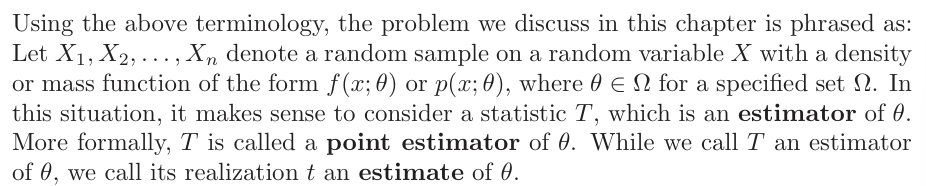
\includegraphics[width=\textwidth]{chap4-20250313.png}
% \caption{}
\label{}
\end{figure}

\begin{figure}[H]
\centering
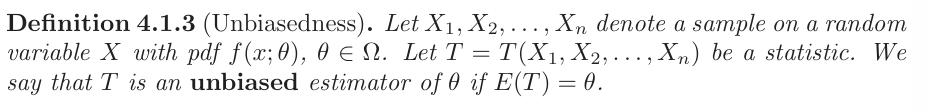
\includegraphics[width=\textwidth]{1-chap4-20250313.png}
% \caption{}
\label{}
\end{figure}

In chapter 6 and 7 we discuss several theories of estimation in general. We briefly discuss the \textbf{maximum likelihood estimator (mle)} and then use it to obtain point estimators. Our discussion is for the continuous case.
The information is involved in the \textbf{likelihood function} $L(\theta)=L(\theta;x_1,\dots,x_n)=\prod_{i=1}^{n}f(x_i;\theta)$. An often-used estimate is the value of $\theta$ that provides a maximum of $L(\theta)$. If unique, this is called the \textbf{maximum likelihood estimator} (mle) and we denote it as $\widehat{\theta}=\mathrm{Argmax}\ L(\theta)$. In practice, it's easier to work with $l(\theta)=\log L(\theta)$, and $\widehat{\theta}$ solves $\frac{ \partial l(\theta) }{ \partial \theta }=0$.

\subsection{Examples}

\subsubsection{Exponential Distribution}

Suppose $X_1,\dots ,X_n\sim\Gamma(1,\theta)$ with density $f(x)=\theta ^{-1}\exp \{ -x/\theta \}$, $0<x<\infty$. The log of the likelihood function is given by
\[
l(\theta)=\log \prod_{i=1}^{n} \frac{1}{\theta} e^{ -x_i/\theta }=-n\log\theta-\theta ^{-1}\sum_{i=1}^{n} x_i
\]
The first partial of the log-likelihood with respect to $\theta$ is
\[
\frac{ \partial l(\theta) }{ \partial \theta } =-n\theta ^{-1}+\theta^{-2}\sum_{i=1}^{n} x_i
\]
Setting this partial to 0 then we obtain the solution $\overline{x}$, thus the statistic $\hat{\theta}=\overline{X}$ is the mle of $\theta$. Because $E(X)=\theta$ we have $E(\overline{X})=\theta$ hence $\hat{\theta}$ is an unbiased estimator of $\theta$.

\subsubsection{Binomial Distribution}

Let $X$ be one of zero. Let $\theta$, $0<\theta<1$, denote the probability of success. Then the pmf of $X$ is
\[
p(x;\theta)=\theta^{x}(1-\theta)^{1-x},\quad x=0\text{ or }1
\]
If $X_1,\dots,X_n$ is a random sample on $X$, then
\[
L(\theta)=\prod_{i=1}^{n} p(x_i;\theta)=\theta^{\sum_{i=1}^{n} x_i}(1-\theta)^{n-\sum_{i=1}^{n}x_i },\quad x_i=0\text{ or }1
\]
Taking logs, we have
\[
l(\theta)=\sum_{i=1}^{n} x_i\log\theta+\left( n-\sum_{i=1}^{n} x_i \right)\log(1-\theta),\quad x_i=0\text{ or }1
\]
The partial derivative of $l(\theta)$ is
\[
\frac{ \partial l(\theta) }{ \partial \theta } =\frac{\sum_{i=1}^{n} x_i}{\theta}-\frac{n-\sum_{i=1}^{n} x_i}{1-\theta}
\]
Thus $\hat{\theta}=\overline{X}$, $E(\widehat{\theta})=E(\overline{X})=\theta$ then $\hat{\theta}$ is an unbiased estimator of $\theta$.

\subsubsection{Normal Distribution}

Let $X_1,\dots,X_n\sim N(\mu,\sigma^{2})$ then $\boldsymbol{\theta}=(\mu,\sigma)$.
\[
l(\mu,\sigma)=-\frac{n}{2}\log2\pi-n\log\sigma-\frac{1}{2}\sum_{i=1}^{n} \left( \frac{x_i-\mu}{\sigma} \right)^{2}
\]
The two partial derivatives simplify to
\[
\begin{aligned}
\frac{ \partial l(\mu,\sigma) }{ \partial \mu }&=-\sum_{i=1}^{n} \left( \frac{x_i-\mu}{\sigma} \right)\left( -\frac{1}{\sigma}  \right) \\
\frac{ \partial l(\mu,\sigma) }{ \partial \sigma }  & =-\frac{n}{\sigma}+\frac{1}{\sigma^{3}}\sum_{i=1}^{n} (x_i-\mu)^{2}   
\end{aligned}
\]
Setting these to 0 and solving simultaneously, we see that the mles are
\[
\hat{\mu}=\overline{X},\quad \hat{\sigma}^{2}=n^{-1}\sum_{i=1}^{n} (X_i-\overline{X})^{2}
\]
We kown that $\overline{X}$ is unbiased estimator for $\mu$ and $S^{2}=\frac{1}{n-1}\sum_{i=1}^{n}(X_i-\overline{X})^{2}$ is an unbiased estimator of $\sigma^{2}$. Thus for the mle of $\sigma^{2}$, $E(\hat{\sigma}^{2})=[n/(n-1)]\sigma^{2}$, which is a biased estimator of $\sigma^{2}$. Note that the bias of $\hat{\sigma}^{2}$ is $E(\hat{\sigma}^{2}-\sigma^{2})=-\sigma^{2}/n$ which converges to 0 as $n\to \infty$. However $S^{2}$ is the preferred estimator of $\sigma^{2}$.

\subsubsection{Uniform Distribution}

Let $X_1,\dots,X_n$ be iid with the uniform $(0,\theta)$ density; i.e.
\[
f(x;\theta)=\frac{1}{\theta}\mathbb{1}_{(0,\theta)}(x) 
\]
Because $\theta$ is in the support, \textbf{differentiation is not helpful} here. The likelihood function can be written as
\[
L(\theta)=\prod_{i=1}^{n} f(x_i;\theta)=\theta^{-n}\prod_{i=1}^{n} \mathbb{1}_{(0,\theta)}(x_i)=\theta^{-n}\mathbb{1}_{(0,\theta)}(\max\{ x_i \})
\]
The function $L(\theta)$ is a decreasing function of $\theta$ for all $\theta\geq \max\{ x_i \}$ and is $0$ otherwise. So the maximum occurs at the smallest value that $\theta$ can assume; i.e. the mle is $\hat{\theta}=\max\{ X_i \}$.

\section{Histogram Estimates of pmfs and pdfs}

In this section we briefly discuss a histogram of the sample, which is an estimate of the pmf, $p(x)$ or the pdf, $f(x)$, of $X$.

\subsubsection{Discrete Distribution}

Assume $X$ discrete with pmf $p(x)$. Let $X_1,\dots,X_n$ be a random sample on $X$. Suppose the space of $X$ is finite, i.e. $\mathcal{D}=\{ a_1,\dots,a_m \}$. An intuitive estimate of $p(a_j)$ is the relative frequency of $a_j$ in the sample.
\[
\widehat{p}(a_j)=\frac{1}{n}\sum_{i=1}^{n} \mathbb{1}_{\{ a_j \}}(X_i)
\]
These estimators $\{ \widehat{p}(a_1),\dots,\widehat{p}(a_m) \}$ constitute the nonparametric estimate of the pmf $p(x)$. Because
\[
E[\widehat{p}(a_j)]=\frac{1}{n}\sum_{i=1}^{n} E[\mathbb{1}_{a_j}(X_i)]=\frac{1}{n}\sum_{i=1}^{n} p(a_j)=p(a_j)
\]
$\widehat{p}(a_j)$ is an unbiased estimator of $p(a_j)$.

Next suppose $X$ infinite, i.e.$\mathcal{D}=\{ a_1,a_2,\dots \}$. In practice, we select a value $a_m$ and make the groupings
\[
\{ a_1 \},\{ a_2 \},\dots,\{ a_m \},\widetilde{a}_{m+1}=\{ a_{m+1},a_{m+2},\dots \}
\]
Let $\widehat{p}(\widetilde{a}_{m+1})$ be the proportion of sample items that are greater than or equal to $a_{m+1}$. Then the estimates $\{ \widehat{p}(a_1),\dots,\widehat{p}(a_m),\widehat{p}(\widetilde{a}_{m+1}) \}$ form our estimate of $p(x)$.

A histogram is a \textbf{barplot} of $\widehat{p}(a_j)$ versus $a_j$. There are two cases to consider. For the first case, supppose the values $a_j$ represent qualitative categories, e.g. hair colors of a population of people. Such histograms are usually called \textbf{bar charts}. An example is helpful here.

\begin{figure}[H]
\centering
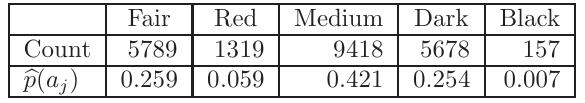
\includegraphics[width=\textwidth]{chap4-20250314.png}
% \caption{}
\label{}
\end{figure}

\begin{figure}[H]
\centering
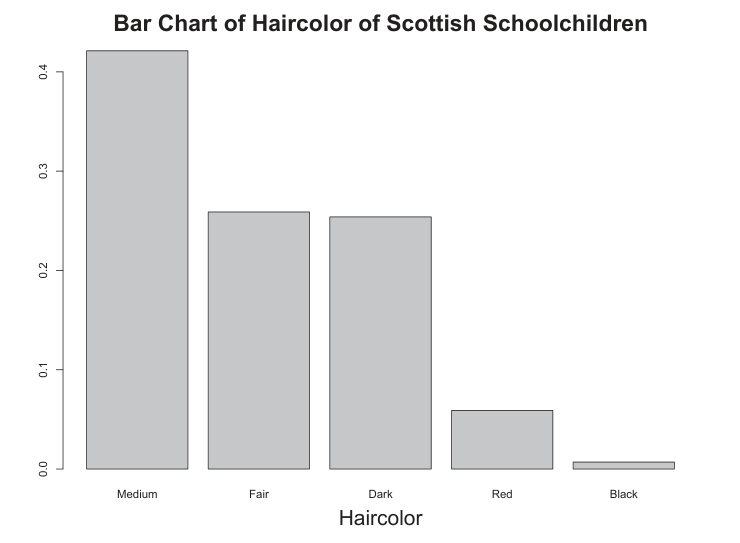
\includegraphics[width=\textwidth]{2-chap4-20250314.png}
% \caption{}
\label{}
\end{figure}

For the second case, assume that the values in the space $\mathcal{D}$ are \textbf{ordinal} in nature; i.e. the natural ordering of the $a_j$ $s$ is numerically meaningful. In this case, the usual histogram is an abutting bar chart with heights $\widehat{p}(a_j)$ that are plotted in the natural order of the $a_j$ $s$, as in the following example.

\begin{figure}[H]
\centering
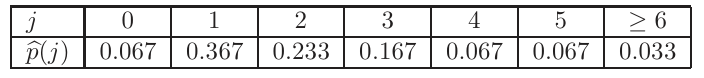
\includegraphics[width=\textwidth]{4-chap4-20250314.png}
% \caption{}
\label{}
\end{figure}

\begin{figure}[H]
\centering
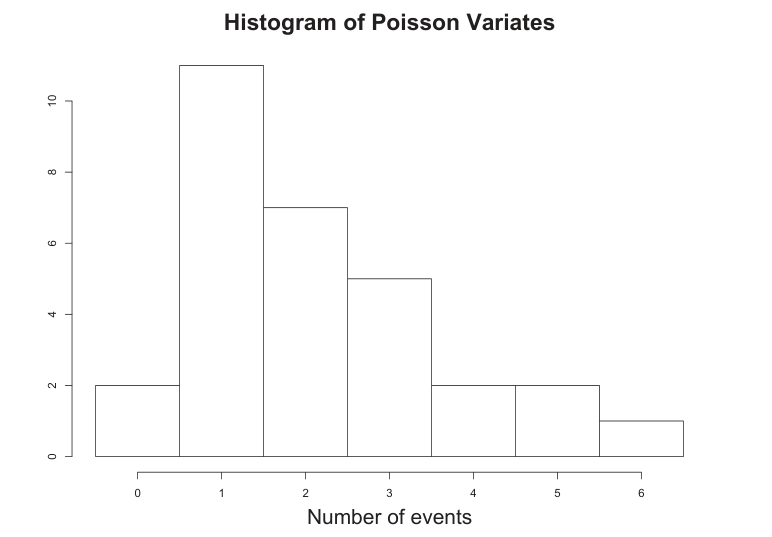
\includegraphics[width=\textwidth]{5-chap4-20250314.png}
% \caption{}
\label{}
\end{figure}

\subsubsection{Continuous Distribution}

For this section, assume that the random sample $X_1,\dots,X_n$ is from a continuous random variable $X$ with continuous pdf $f(t)$. For an arbitrary but fixed point $x$ and a given $h>0$, consider the interval $(x-h,x+h)$. By the mean value theorem for integrals, we have for some $\xi$, $\lvert x-\xi \rvert<h$, that
\[
P(x-h<X<x+h)=\int_{x-h}^{x+h} f(t) \, dt =f(\xi)2h\approx f(x)2h
\]
Let the sample items fall in $(x-h,x+h)$, which suggests the following nonparmetric extimate of $f(x)$ at a given $x$:
\[
\widehat{f}(x)=\frac{\#\{ x-h<X_i<x+h \}}{2hn}
\]
More formally, a nonparametric estimator of $f(x)$ is
\[
\widehat{f}(x)=\frac{1}{2hn}\sum_{i=1}^{n} \mathbb{1}_{(x-h,x+h)}(X_i)
\]
Then
\[
E[\widehat{f}(x)]=\frac{1}{2hn}\sum_{i=1}^{n} E[\mathbb{1}_{(x-h,x+h)}(X_i)]=\frac{1}{2hn}\sum_{i=1}^{n} P(X_i\in(x-h,x+h))=\frac{1}{2hn}nf(\xi)2h=f(\xi)\to f(x)\quad \text{as }h\to0
\]
Hence $\widehat{f}(x)$ is approximately an unbiased estimator of the density $f(x)$.

\begin{figure}[H]
\centering
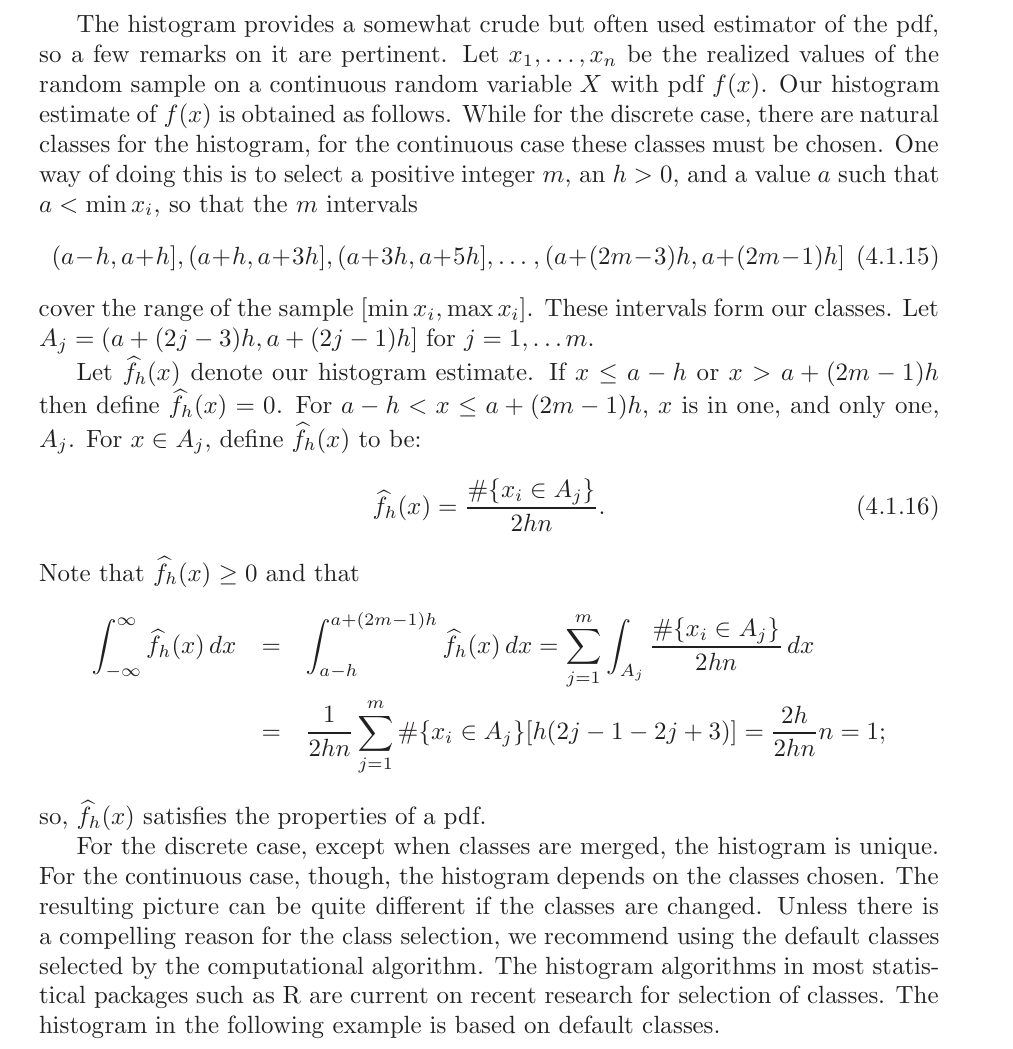
\includegraphics[width=\textwidth]{6-chap4-20250314.png}
% \caption{}
\label{}
\end{figure}

\section{Confidence Intervals}

Recall that the random variable of interest $X$ has density $f (x;\theta),\theta\in \Omega$, where $\theta$ is unknown. In Section 4.1, we discussed estimating $\theta$ by a statistic $\widehat{\theta}=\widehat{\theta}(X_1,\dots,X_n)$, where $X_1,\dots,X_n$ is a sample from the distribution of $X$. But how much did $\widehat{\theta}$ miss $\theta$? In this section, we embody this estimate of error in terms of a confidence interval, which we now formally define:

\begin{figure}[H]
\centering
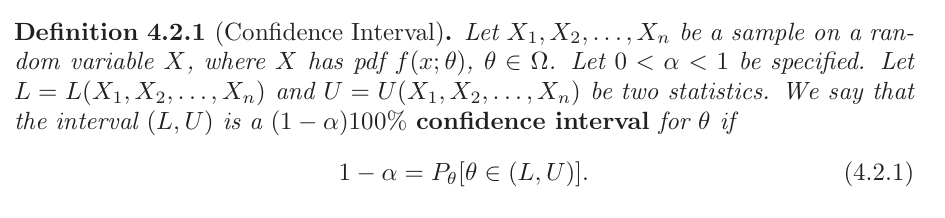
\includegraphics[width=\textwidth]{7-chap4-20250314.png}
% \caption{}
\label{}
\end{figure}

\begin{figure}[H]
\centering
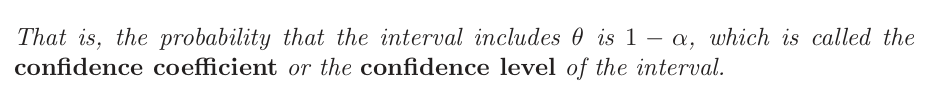
\includegraphics[width=\textwidth]{8-chap4-20250314.png}
% \caption{}
\label{}
\end{figure}

\begin{figure}[H]
\centering
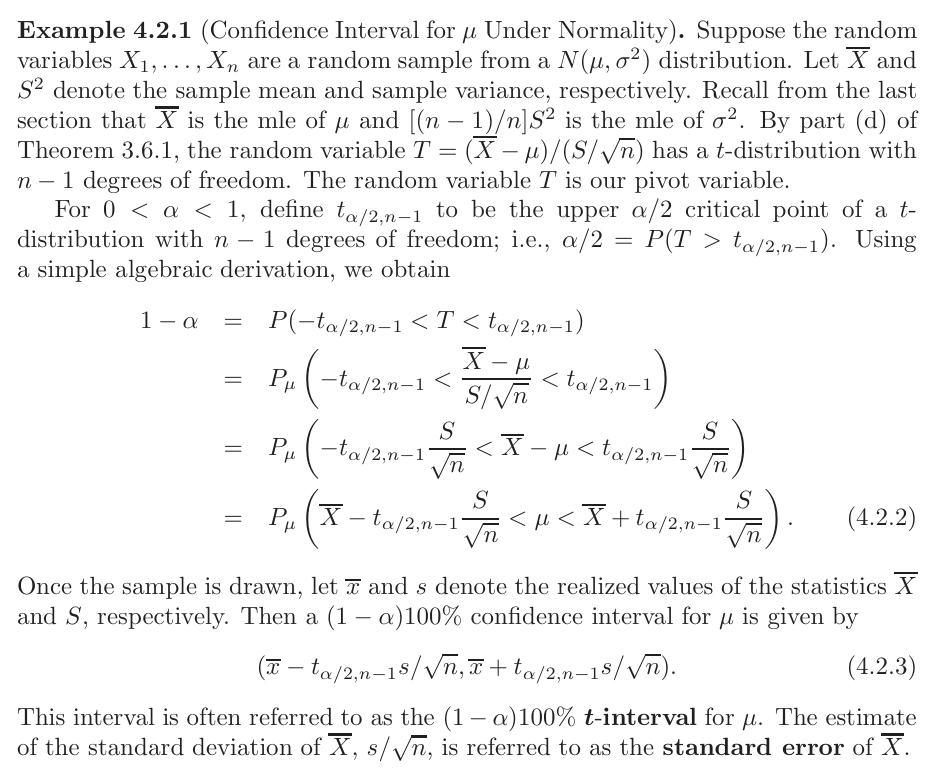
\includegraphics[width=\textwidth]{11-chap4-20250314.png}
% \caption{}
\label{}
\end{figure}

For $0<\alpha<1$, define $\alpha/2=P(Z>z_{\alpha/2 })$ for $Z\sim N(0,1)$.

Motivated by the CLT, we have
\begin{figure}[H]
\centering
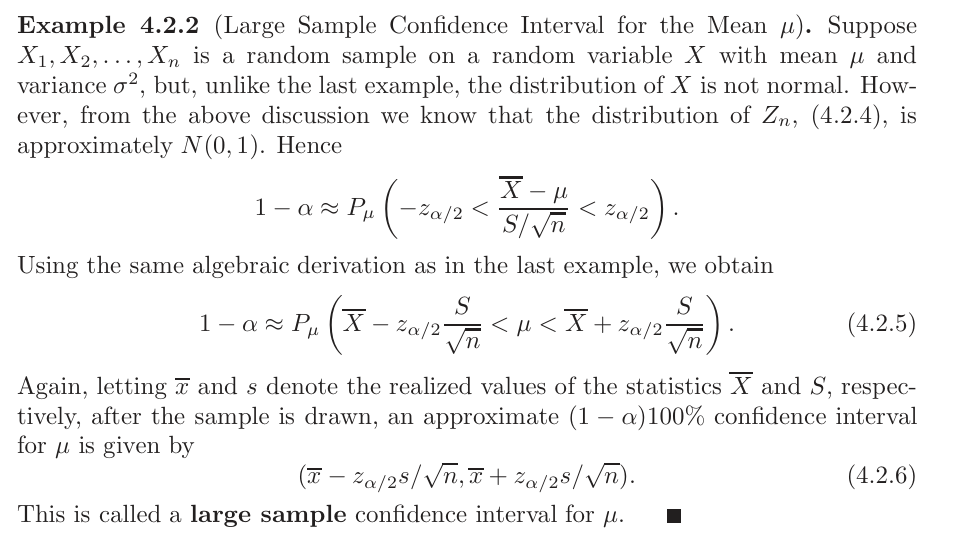
\includegraphics[width=\textwidth]{9-chap4-20250314.png}
% \caption{}
\label{}
\end{figure}

\begin{figure}[H]
\centering
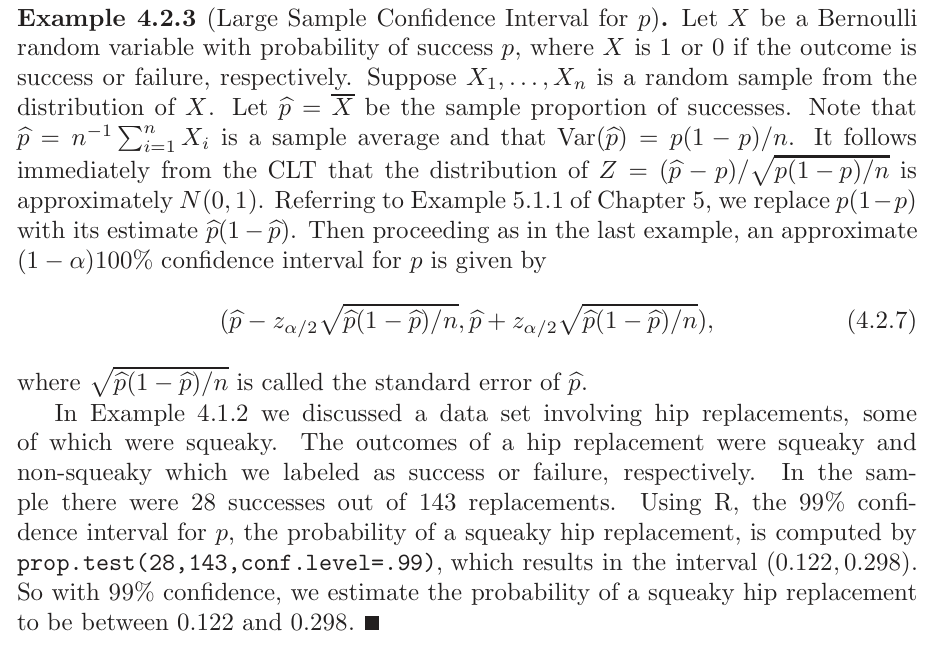
\includegraphics[width=\textwidth]{10-chap4-20250314.png}
% \caption{}
\label{}
\end{figure}

\subsection{Confidence Intervals for Difference in Means}

A practical problem of interest is the comparison of two distributions, $X$ and $Y$. In this section, we compare the means of $X$ and $Y$, denoted by $\mu_1$ and $\mu_2$. In particular, we obtain confidence intervals for the difference $\Delta=\mu_1-\mu_2$. Let $X_1,\dots,X_{n_1}$ be a random sample from the distribution of $X$ and $Y_1,\dots,Y_{n_2}$ from $Y$, and all independent of one another. Let $\overline{X}=n_1 ^{-1}\sum_{i=1}^{n_1}X_i$ and $\overline{Y}=n_2^{-1}\sum_{i=1}^{n_2}Y_i$ and $\widehat{\Delta}=\overline{X}-\overline{Y}$, which is an unbiased estimator of $\Delta$. This difference $\widehat{\Delta}-\Delta$ is the numerator of the pivot random variable. By independence of the samples,
\[
\mathrm{Var}(\widehat{\Delta})=\frac{\sigma_1^{2}}{n_1}+\frac{\sigma_2^{2}}{n_2}
\]
Let $S_1^{2}=(n_1-1)^{-1}\sum_{i=1}^{n_1}(X_i-\overline{X})^{2}$ and $S_2^{2}=(n_2-1)^{-1}\sum_{i=1}^{n_2}(Y_i-\overline{Y})^{2}$ be the sample variances. Then estimating the variances by the sample variances, consider the random variable
\[
Z=\frac{\widehat{\Delta}-\Delta}{\sqrt{ \frac{S_1^{2}}{n_1} +\frac{S_2^{2}}{n_2}}}
\]
By CLT, this pivot variable has an approximate $N(0,1)$ distribution. This leads to the approximate $(1-\alpha) 100\%$ confidence interval for $\Delta=\mu_1-\mu_2$ given by
\[
\left( (\overline{x}-\overline{y})-z_{\alpha/2}\sqrt{ \frac{s_1^{2}}{n_1}+\frac{s_2^{2}}{n_2} }, (\overline{x}-\overline{y})+z_{\alpha/2}\sqrt{ \frac{s_1^{2}}{n_1}+\frac{s_2^{2}}{n_2} }\right)
\]
where $\sqrt{ (s_1^{2}/n_1)+(s_2^{2}/n_2) }$ is the standard error of $\overline{X}-\overline{Y}$. This is a large sample $(1-\alpha) 100\%$ confidence interval for $\mu_1-\mu_2$.

\begin{figure}[H]
\centering
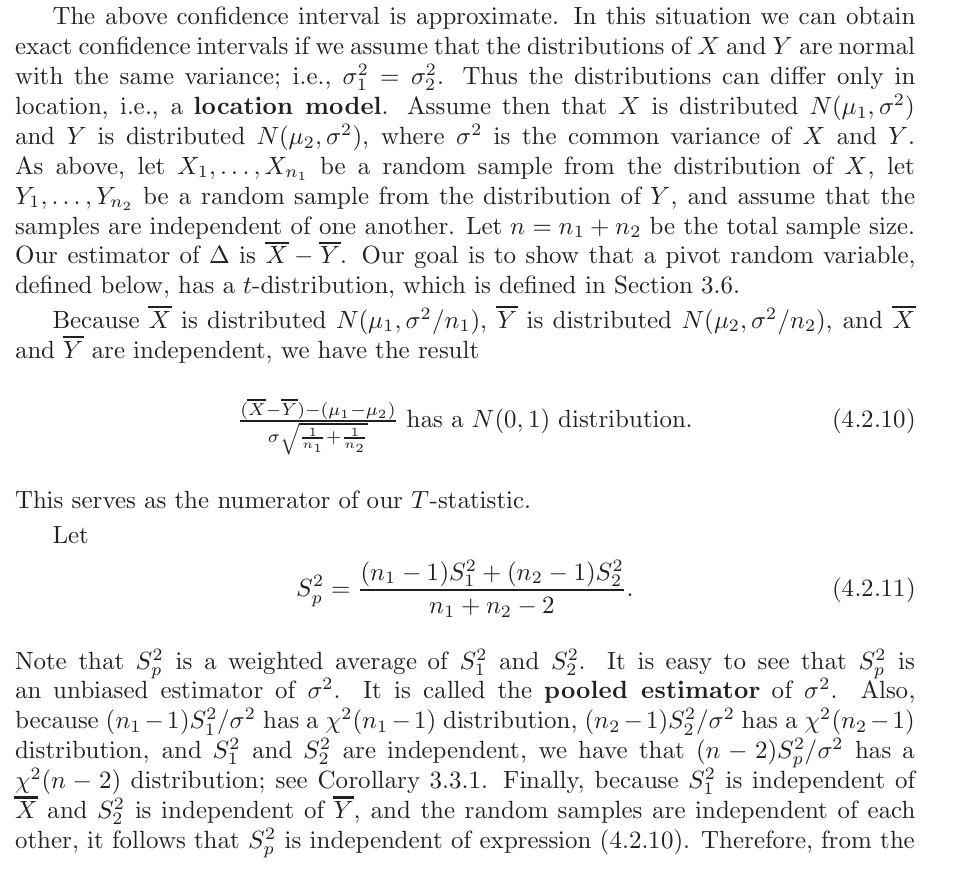
\includegraphics[width=\textwidth]{12-chap4-20250314.png}
% \caption{}
\label{}
\end{figure}

\begin{figure}[H]
\centering
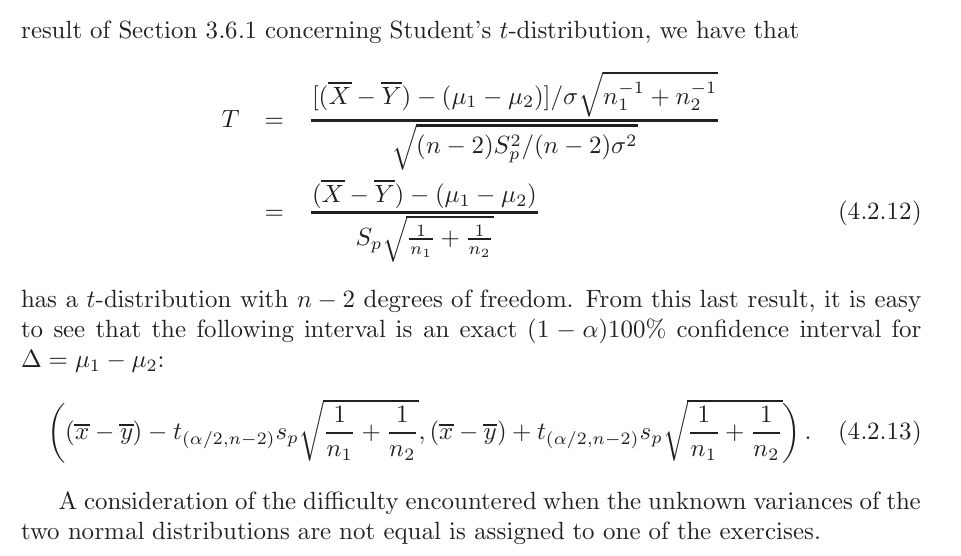
\includegraphics[width=\textwidth]{13-chap4-20250314.png}
% \caption{}
\label{}
\end{figure}

\subsection{Confidence Interval for Difference in Proportions}

Omitted...

\subsection{Confidence Intervals for Parameters of Discrete Distributions}

Omitted...

\section{Order Statistics}

\begin{definition}[order statistic]
\begin{figure}[H]
\centering
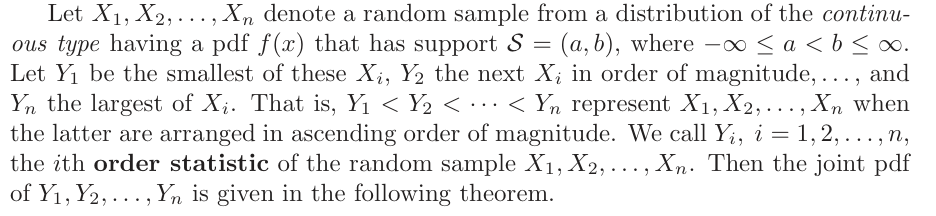
\includegraphics[width=\textwidth]{14-chap4-20250314.png}
% \caption{}
\label{}
\end{figure}
\end{definition}
\begin{figure}[H]
\centering
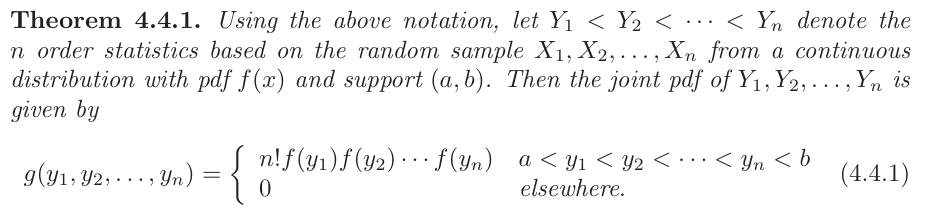
\includegraphics[width=\textwidth]{15-chap4-20250314.png}
% \caption{}
\label{}
\end{figure}

Note that the support of $X_1,\dots,X_n$ an be partitioned into $n!$ mutually disjoint sets that map onto the support of $Y_1,\dots,Y_n$ namely, $\{ (y_1,\dots,y_n):a<y_1<\dots<y_n<b \}$. One of these $n!$ sets is $a<x_1<\dots<x_n<b$, and the others can be found by permuting the $n$ $x$ s in all possible way, thus the Jacobian equal to 1.
\[
g(y_1,\dots,y_n)=\sum_{i=1}^{n!} \lvert J_i \rvert f(y_1)\dots f(y_n)=\begin{cases}
n!f(y_1)\dots f(y_n) & a<y_1<\dots<y_n<b \\
0 & \text{elsewhere}
\end{cases}
\]
\begin{figure}[H]
\centering
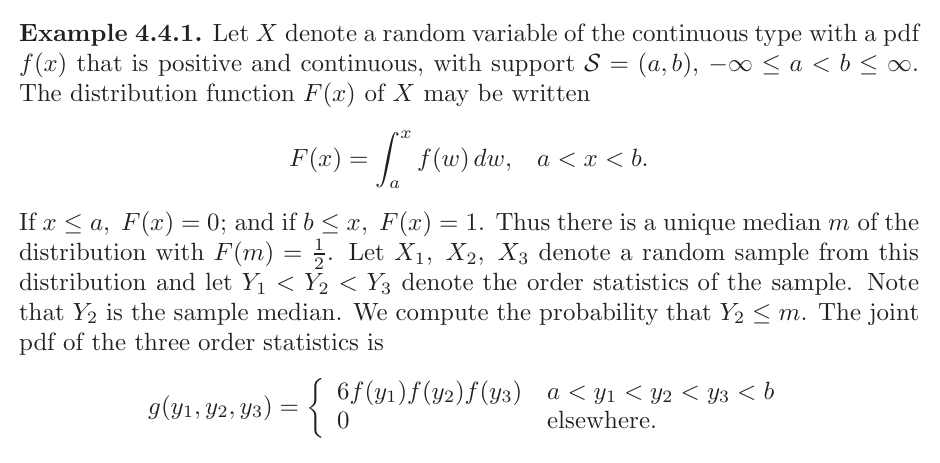
\includegraphics[width=\textwidth]{16-chap4-20250314.png}
% \caption{}
\label{}
\end{figure}

\begin{figure}[H]
\centering
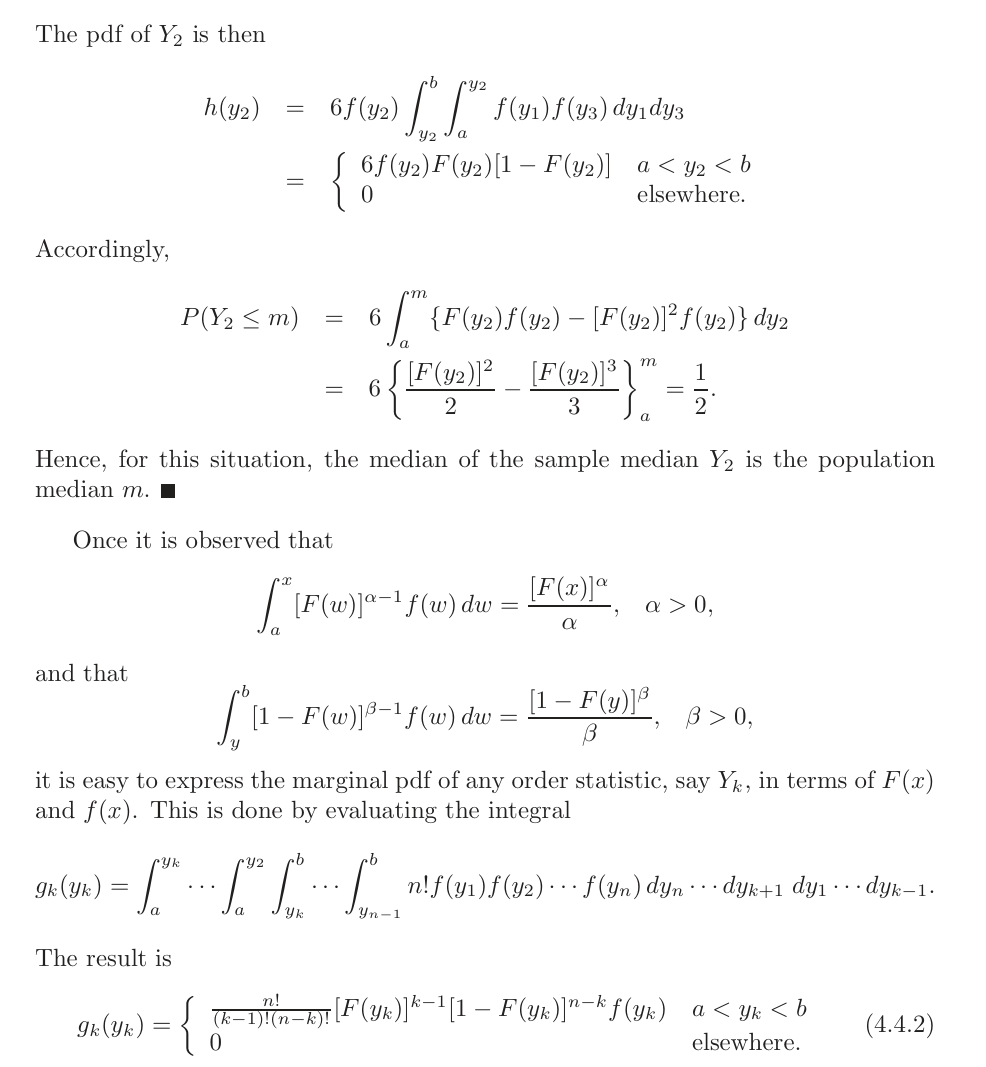
\includegraphics[width=\textwidth]{17-chap4-20250314.png}
% \caption{}
\label{}
\end{figure}

Omitted...

\subsection{Quantiles}

\subsection{Confidence Intervals for Quantiles}

$X$ continuous rv with cdf $F(x)$. For $0<p<1$, define the $100p$ th distribution percentile to be $\xi_{p}$, where $F(\xi_{p})=p$. Let $Y_1<\dots<Y_n$ be the order statistics. Then
\[
P(Y_i<\xi_{p}<Y_j)=\sum_{w=i}^{j-1} \binom{n}{w}p^{w}(1-p)^{n-w}\eqqcolon \gamma
\]
Then $(y_i,y_j)$ serves as a $100\gamma\%$ confidence interval for $\xi_{p}$, the quantile of order $p$.

\subsubsection{Confidence Interval for the Median}

\begin{figure}[H]
\centering
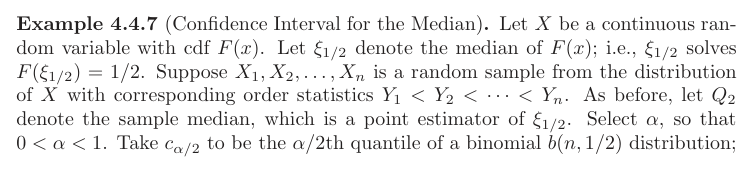
\includegraphics[width=\textwidth]{chap4-2025033022.png}
% \caption{}
\label{}
\end{figure}
\begin{figure}[H]
\centering
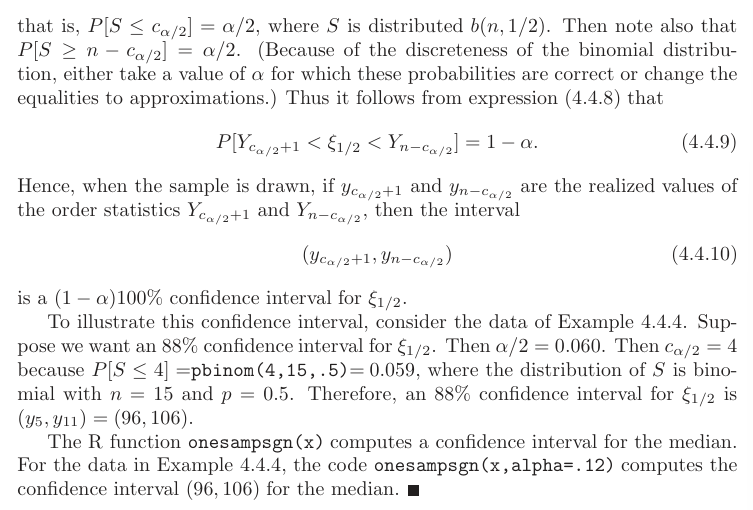
\includegraphics[width=\textwidth]{1-chap4-2025033022.png}
% \caption{}
\label{}
\end{figure}

\section{Introduction to Hypothesis Testing}

See All of statistics Chapter 10.

\subsection{Definitions of critical (rejection) region, power function, size (significance level), level, type I (II) error, two-side test, one-side test}

We partition the parameter space $\Theta$ into two disjoint sets $\Theta_0$ and $\Theta_1$ and we wish to test
\[
H_0:\theta\in\Theta_0\qquad \text{versus}\qquad H_1:\theta\in\Theta_1
\]
We call $H_0$ the \textbf{null hypothesis} and $H_1$ the \textbf{alternative hypothesis}. Let $X$ be a r.v. and $\mathcal{X}$ be the range of $X$. To test a hypothesis, we aim to find the \textbf{rejection region}(critical region) $R\subset \mathcal{X}$. If $X\in R$ we reject $H_0$, otherwise retain $H_0$.

\begin{definition}[critical region (rejection region)]
A test of $H_0$ versus $H_1$ is based on a subset $C$ of $\mathcal{D}$. This set $C$ is called the \textbf{critical region (rejection region)} and its corresponding decision rule (test) is
\[
\begin{aligned} \text { Reject } H_0\left(\text { Accept } H_1\right) &\qquad  \text { if }\left(X_1, \ldots, X_n\right) \in C \\ \text { Retain } H_0\left(\text { Reject } H_1\right) & \qquad \text { if }\left(X_1, \ldots, X_n\right) \in C^c .\end{aligned}
\]
\end{definition}
Usually, the \textbf{rejection region} $R$ (critical region $C$) is of the form
\[
R=\{ x:T(x)>c \}
\]
where $T$ is a \textbf{test statistic} and $c$ is called a \textbf{critical value}.

\begin{definition}[power function, size (significance level), level]
The \textbf{power function} of a test with rejection region $R$ is defined by
\[
\beta(\theta)=\mathbb{P}_{\theta}(X\in R)
\]
The \textbf{size} of a test is defined to be
\[
\alpha=\sup_{\theta\in\Theta_0}\beta(\theta)
\]
A test is said to have \textbf{level}\footnote{The definition is useless.} $\alpha$ if its size is less than or equal to $\alpha$.
\end{definition}
\begin{definition}[type I error, type II error]
Rejecting $H_0$ when $H_0$ is true is called a \textbf{type I error}. Retaining $H_0$ when $H_1$ is true is called a \textbf{type II error}.
\end{definition}
\begin{definition}[two-side test, one-side test]
A test of the form
\[
H_0:\theta=\theta_0\qquad \text{versus}\qquad H_1:\theta\neq \theta_0
\]
is called a \textbf{two-side test}. A test of the form
\[
H_0:\underset{ \text{or }\geq  }{ \theta\leq \theta_0 }\qquad \text{versus}\qquad H_1:\underset{ \text{or }< }{ \theta>\theta_0 }
\]
is called a \textbf{one-side test}. The most common tests are two-sided.
\end{definition}
\subsubsection{Example}

\begin{figure}[H]
\centering
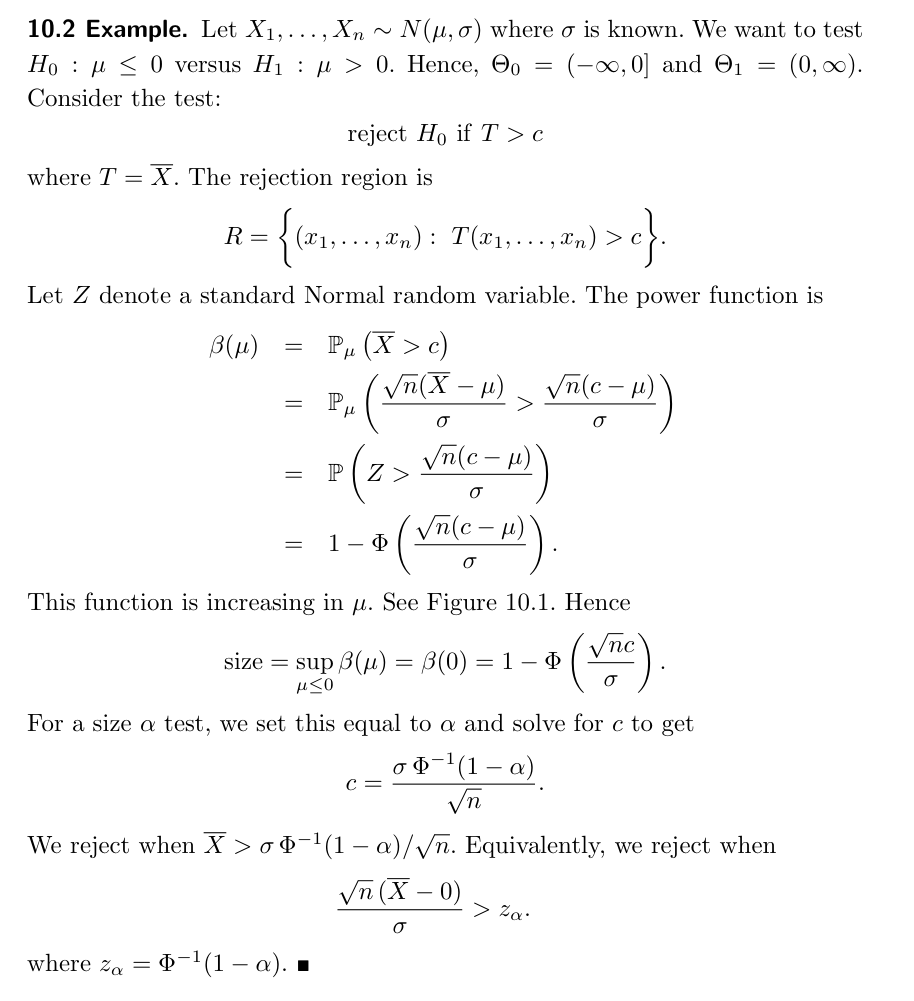
\includegraphics[width=\textwidth]{4-chap4-2025040315.png}
% \caption{}
\label{}
\end{figure}

\begin{figure}[H]
\centering
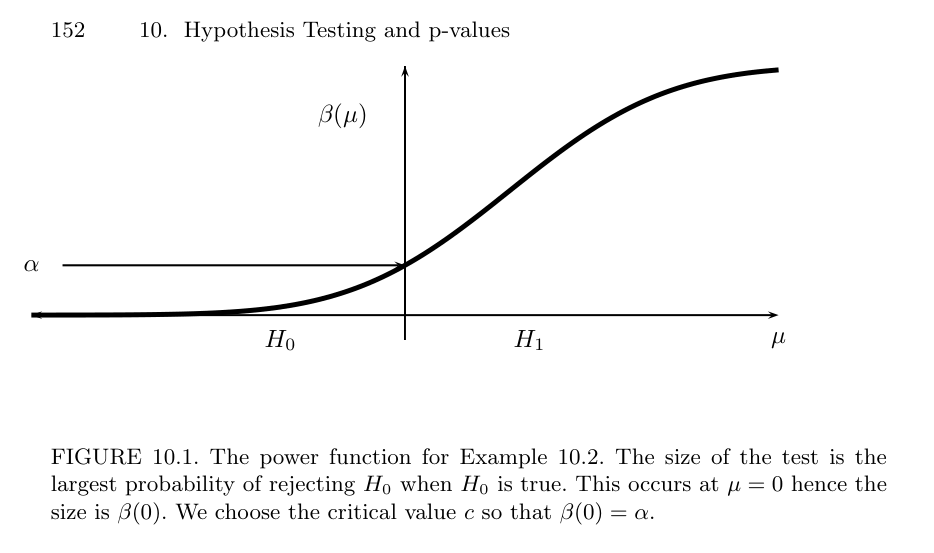
\includegraphics[width=\textwidth]{5-chap4-2025040315.png}
% \caption{}
\label{}
\end{figure}

Next we consider four widely used tests: the Wald test, the $\chi^{2}$ test, the permutation test, and the likelihood ratio test.

\subsection{The Wald test}

Let $\theta$ be a scalar parameter, let $\widehat{\theta}$ be an estimate of $\theta$ and let $\widehat{\text{se}}$ be the estimated standard error of $\widehat{\theta}$.

\begin{definition}[The Wald Test]
Consider testing $H_0:\theta=\theta_0,H_1:\theta\neq\theta_0$. Assume that the estimator $\widehat{\theta}$ is asymptotically Normal, i.e.
\[
W\coloneqq \frac{\widehat{\theta}-\theta_0}{\widehat{\text{se}}}\overset{ \mathcal{D} }{ \to }N(0,1)
\]
The size $\alpha$ \textbf{Wald test} is: reject $H_0$ when $\lvert W \rvert>z_{\alpha/2}$.
\end{definition}
$z_{\alpha}$ means that for $Z\sim N(0,1)$,
\[
\mathbb{P}(Z>z_{\alpha})=\alpha
\]
Thus
\[
z_{\alpha}\coloneqq \Phi ^{-1}(1-\alpha)
\]
where $\Phi(x)=\mathbb{P}(Z\leq x)=F_{Z}(x)$.

\begin{remark}
An alternative version of the Wald test statistic is $W=(\widehat{\theta}-\theta_0)/\widehat{\text{se}_{0}}$ where $\text{se}_{0}$ is the standard error computed at $\theta=\theta_0$. Both versions of the test is valid.
\end{remark}
Let us consider the power of the Wald test when the null hypothesis is false.
\begin{figure}[H]
\centering
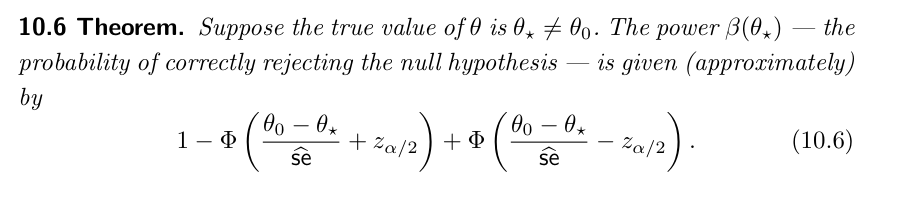
\includegraphics[width=\textwidth]{9-chap4-2025040315.png}
% \caption{}
\label{}
\end{figure}

\begin{theorem}[The rejection region of size $\alpha$ Wald test]
The size $\alpha$ Wald test rejects $H_0:\theta=\theta_0$ versus $H_1:\theta\neq\theta_0$ iff $\theta_0 \not\in C$ where
\[
C=(\widehat{\theta}-\widehat{\text{se}}\cdot z_{\alpha/2},\widehat{\theta}+\widehat{\text{se}}\cdot z_{\alpha/2})
\]
Thus, testing the typothesis is equivalent to checking whether the null value is in the confidence interval.
\end{theorem}
\begin{remark}
When we reject $H_0$ we often say that the result is statistically significant.
\end{remark}
\subsubsection{Example 1}

\begin{figure}[H]
\centering
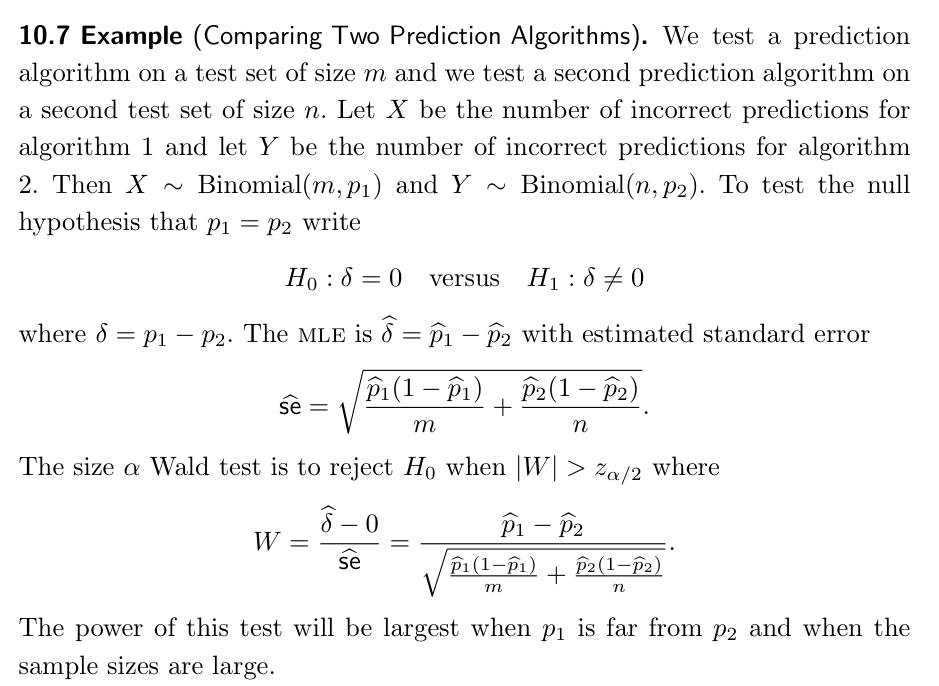
\includegraphics[width=\textwidth]{5-chap4-2025041621.png}
% \caption{}
\label{}
\end{figure}

\subsubsection{Example 2}

\begin{figure}[H]
\centering
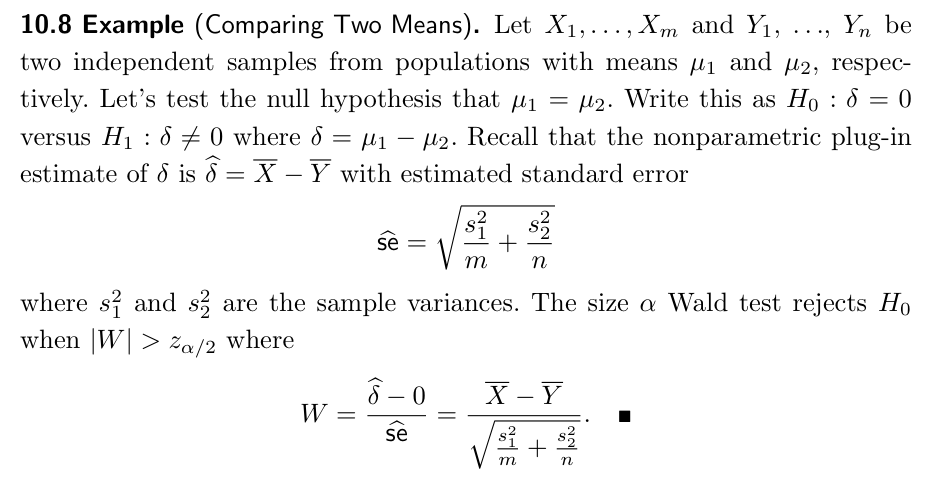
\includegraphics[width=\textwidth]{6-chap4-2025041621.png}
% \caption{}
\label{}
\end{figure}

\subsection{\texorpdfstring{$p$}{p} -values}

For every $\alpha\in(0,1)$ we have a size $a$ test with rejection region $R_{\alpha}$. Then
\[
\text{p-value}=\inf \{ \alpha:T(X)\in R_{\alpha} \}
\]
$p$ -value is the smallest level at which we can reject $H_0$.

\begin{remark}
Do not confuse the $p$ -value with $\mathbb{P}(H_0|\text{Data})$. The $p$ -value is not the probability that the null hypothesis is true.
\end{remark}
Suppose that the size $\alpha$ test is of the form
\[
\text{reject  }H_0\qquad \text{iff}\qquad T(X)\geq c_{\alpha}
\]
Then
\[
\text{p-value}=\sup_{\theta\in\Theta_0}\mathbb{P}_{\theta}(T(X)>T(x))
\]
where $x$ is the observed value of $X$.

\begin{note}
The $p$ -value is the probability (under $H_0$) of observing a value of the test statistic the same as or more extreme than what was actually observed.
\end{note}
\subsubsection{Example}

\begin{figure}[H]
\centering
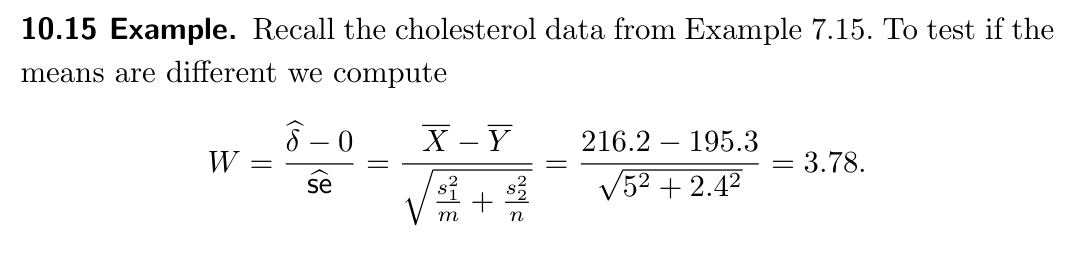
\includegraphics[width=\textwidth]{3-chap4-2025040316.png}
% \caption{}
\label{}
\end{figure}
\begin{figure}[H]
\centering
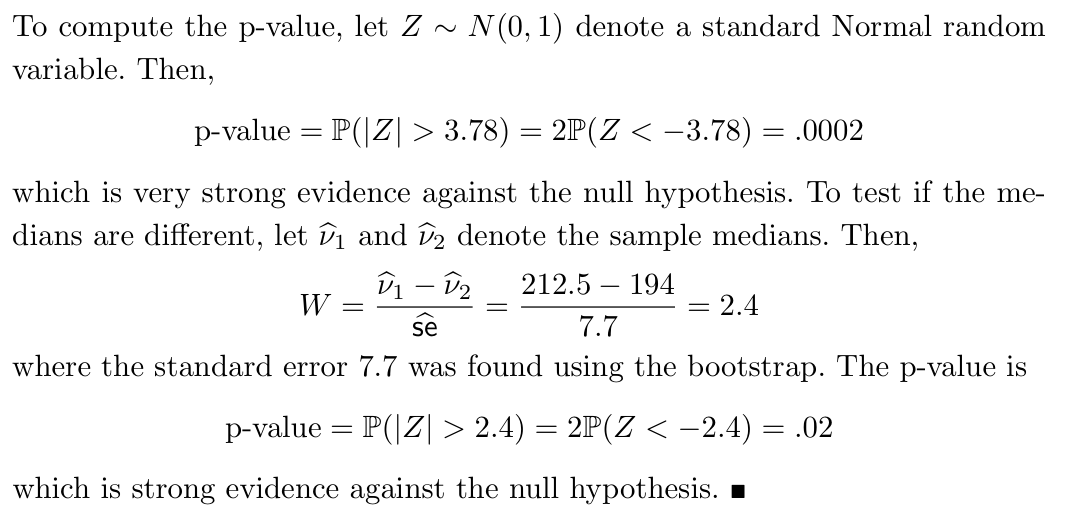
\includegraphics[width=\textwidth]{4-chap4-2025040316.png}
% \caption{}
\label{}
\end{figure}

\subsection{\texorpdfstring{$\chi^{2}$}{chi^2} test}

\subsubsection{Definition of \texorpdfstring{$\chi^{2}$}{chi^2} distribution}

\begin{figure}[H]
\centering
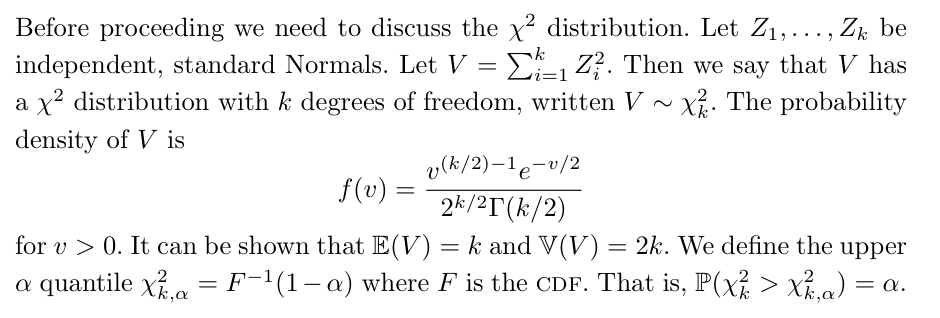
\includegraphics[width=\textwidth]{chap4-2025041621.png}
% \caption{}
\label{}
\end{figure}

\subsubsection{Pearson's \texorpdfstring{$\chi^{2}$}{chi^2} test for multinomial data}

The Pearson's $\chi^{2}$ test is used for multinomial data. If $X=(X_1,\dots,X_k)$ has a multinomial $(n,p)$ distribution, then the MLE of $p$ is $\widehat{p}=(\widehat{p}_{1},\dots,\widehat{p}_k)$

\begin{note}
$X_1,\dots,X_k$ need not to be independent!
\end{note}
\begin{definition}[Pearson's $\chi^{2}$ statistic]
\textbf{Pearson's $\chi^{2}$ statistic} is
\[
T=\sum_{j=1}^{k} \frac{(X_j-np_{0j})^2}{np_{0j}}=\sum_{j=1}^{k}\frac{(X_j-E_j)^2}{E_j} 
\]
where $E_j=\mathbb{E}(X_j)=np_{0j}$ is the expected value of $X_j$ under $H_0$.
\end{definition}
Under $H_0$, $T \rightsquigarrow \chi_{k-1}^2$. Hence the test: reject $H_0$ if $T>$ $\chi_{k-1, \alpha}^2$ has asymptotic level $\alpha$. The p-value is $\mathbb{P}\left(\chi_{k-1}^2>t\right)$ where $t$ is the observed value of the test statistic.

\begin{figure}[H]
\centering
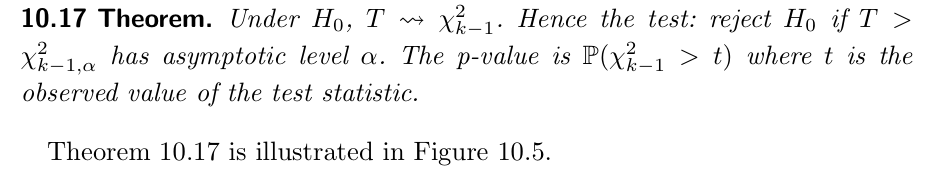
\includegraphics[width=\textwidth]{2-chap4-2025041621.png}
% \caption{}
\label{}
\end{figure}

\paragraph{Example}

\begin{figure}[H]
\centering
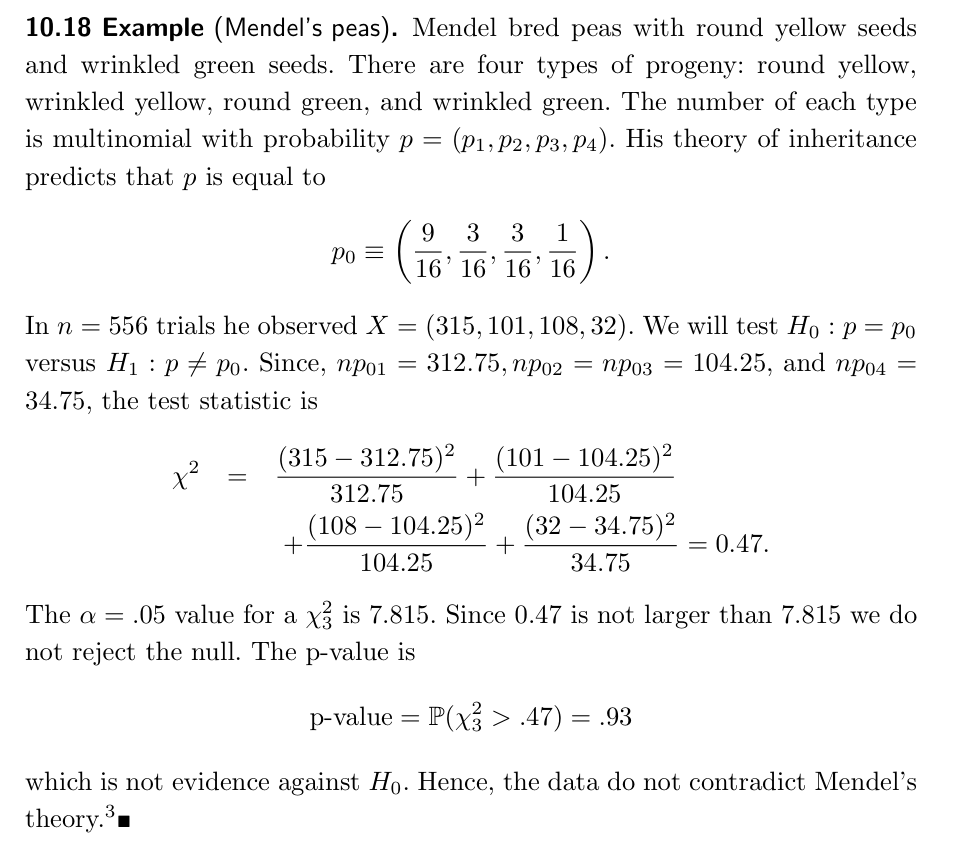
\includegraphics[width=\textwidth]{4-chap4-2025041621.png}
% \caption{}
\label{}
\end{figure}

\subsubsection{Goodness-of-fit test (\texorpdfstring{$H_0:$}{H_0:} \texorpdfstring{$Y$}{Y} satisfies some distribution)}

\begin{figure}[H]
\centering
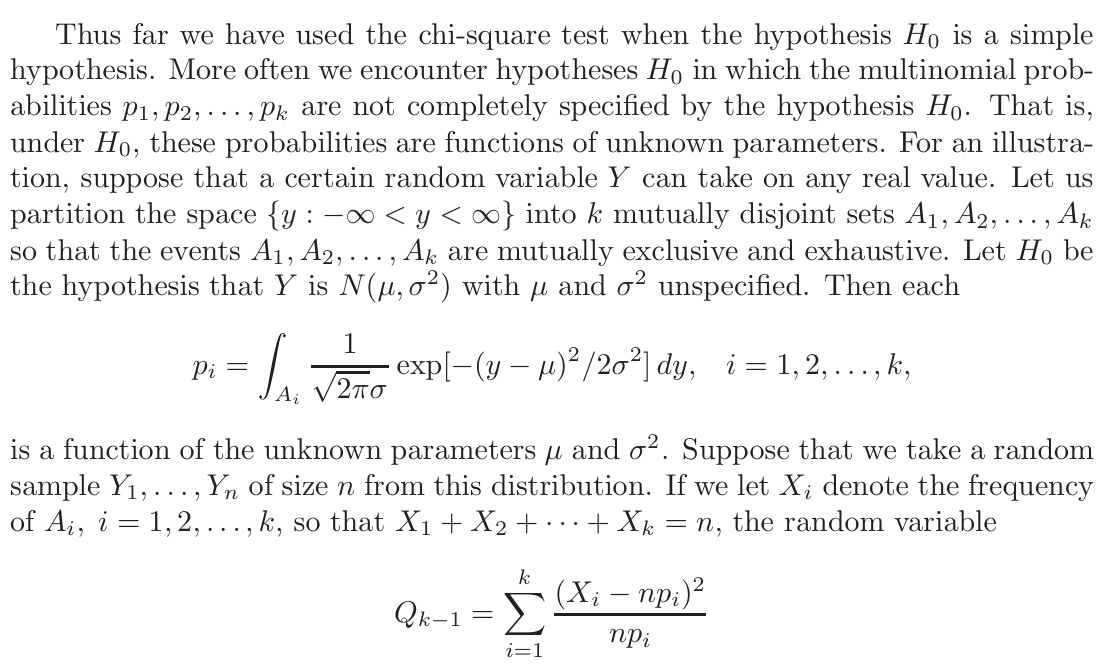
\includegraphics[width=\textwidth]{1-chap4-2025041712.png}
% \caption{}
\label{}
\end{figure}
\begin{figure}[H]
\centering
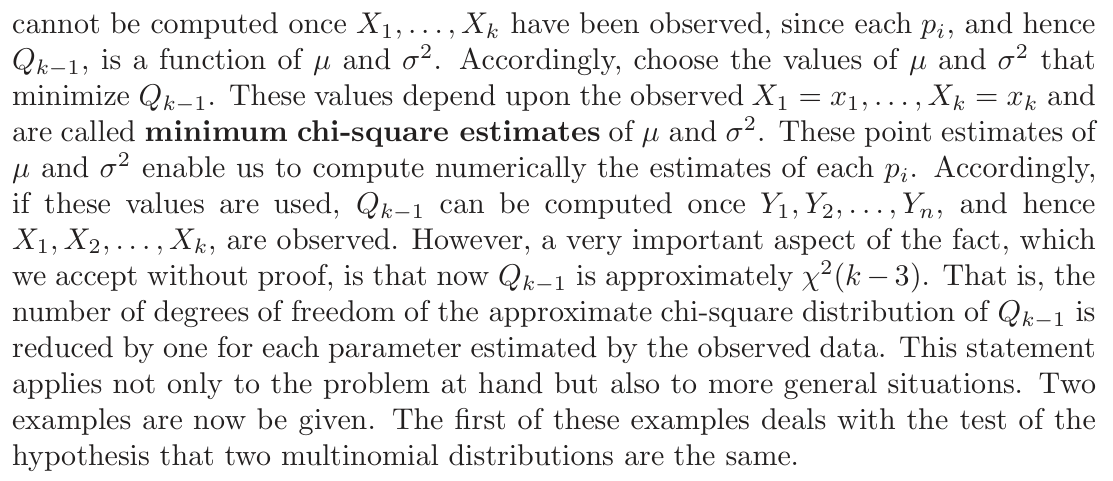
\includegraphics[width=\textwidth]{2-chap4-2025041712.png}
% \caption{}
\label{}
\end{figure}

\section{Consistency and Limiting Distributions}

\subsection{Convergence in Probability}

In this section, we formalize the notion of a sequence of random variables $\{X_n\}$ getting "close" to another random variable $X$ as $n \to \infty$. We say $X_n$ \textbf{converges in probability} to $X$, denoted as $X_n \overset{P}{\to} X$, if $P(|X_n - X| \geq \epsilon) \to 0$ for all $\epsilon > 0$.

One way to demonstrate convergence in probability is to use Chebyshev's Theorem: for a random variable $X$ with variance $\sigma^2 < \infty$, and for any $k > 0$, we have $P(|X - \mu| \geq k\sigma) \leq \frac{1}{k^2}$.

Let $\{X_n\}$ be a sequence of independent and identically distributed (i.i.d.) random variables with mean $\mu$ and variance $\sigma^2 < \infty$. Let $\overline{X}_n = \frac{1}{n} \sum_{i=1}^n X_i$. Then $\overline{X}_n \overset{P}{\to} \mu$.

\begin{proof}
The mean and variance of $\overline{X}_n$ are $\mu$ and $\frac{\sigma^2}{n}$, respectively. By Chebyshev's Theorem, for all $\epsilon > 0$, we have
\[
P(|\overline{X}_n - \mu| \geq \epsilon) = P\left(|\overline{X}_n - \mu| \geq \frac{\epsilon \sqrt{n}}{\sigma} \cdot \frac{\sigma}{\sqrt{n}}\right) \leq \frac{\sigma^2}{n\epsilon^2} \to 0.
\]
\end{proof}

The Weak Law of Large Numbers (WLLN) implies that all the mass of the distribution of $\overline{X}_n$ converges to $\mu$. In a sense, for large $n$, $\overline{X}_n$ is close to $\mu$. But how close is it? For example, if we were to estimate $\mu$ by $\overline{X}_n$, what can we say about the error of estimation? Actually, a Strong Law of Large Numbers (SLLN) can be proved. Moreover, we can weaken the hypothesis of the WLLN to require only that the $X_i$ are i.i.d. with finite mean $\mu$. Thus, the SLLN is a first moment theorem, while the WLLN requires the existence of the second moment.

Next, we list several theorems concerning convergence in probability, which is closed under linearity.

\begin{theorem}
Suppose $X_n \overset{P}{\to} X$ and $Y_n \overset{P}{\to} Y$. Then $X_n + Y_n \overset{P}{\to} X + Y$.
\end{theorem}
\begin{proof}
Using the triangle inequality, we have
\[
P(|(X_n + Y_n) - (X + Y)| \geq \epsilon) \leq P(|X_n - X| + |Y_n - Y| \geq \epsilon) \leq P\left(|X_n - X| \geq \frac{\epsilon}{2}\right) + P\left(|Y_n - Y| \geq \frac{\epsilon}{2}\right).
\]
\end{proof}

\begin{theorem}
For any constant $a$, if $X_n \overset{P}{\to} X$, then $aX_n \overset{P}{\to} aX$.
\end{theorem}
\begin{theorem}
If $X_n \overset{P}{\to} a$ and the real function $g$ is continuous at $a$, then $g(X_n) \overset{P}{\to} g(a)$.
\end{theorem}
\begin{proof}
Since $g$ is continuous at $a$, for all $\epsilon > 0$, there exists $\delta > 0$ such that $|g(x) - g(a)| < \epsilon$ for $|x - a| < \delta$. Thus, $|g(x) - g(a)| \geq \epsilon$ implies $|x - a| \geq \delta$. Substituting $X_n$ for $x$, we obtain
\[
P(|g(X_n) - g(a)| \geq \epsilon) \leq P(|X_n - a| \geq \delta) \to 0.
\]
\end{proof}

\begin{exercise}
If $X_n\overset{ P }{ \to }X$, then $g(X_n)\overset{ P }{ \to }g(X)$ for continuous $g$ over $\mathbb{R}$.
\end{exercise}
\begin{proof}
For r.v. $X$, since $F_{X}(x)\to0$ as $x\to-\infty$ and $F_{Y}(x)\to1$ as $x\to+\infty$, $X$ is $\mathbb{P}$ -bounded. Given $\epsilon>0$, since $X_n\overset{ P }{ \to }X$, $\exists N>0$, s.t. $\mathbb{P}(\lvert X_n-X \rvert\geq1)<\epsilon$ for $n\geq N$ and $\exists M>0$, s.t. $\mathbb{P}(\lvert X \rvert\geq M)<\epsilon$, thus $\mathbb{P}(\lvert X_n \rvert\geq M+1)\leq \mathbb{P}(\lvert X_n-X \rvert\geq1)+\mathbb{P}(\lvert X \rvert\geq M)<2\epsilon$ for $n\geq N$.

As $g$ is continuous on $[-M-1,M+1]$, thus uniformly continuous, then  $\forall \eta>0,\exists\delta>0$, s.t. for $x, y\in[-M-1,M+1]$ $\lvert x-y \rvert<\delta\Rightarrow \lvert g(x)-g(y) \rvert<\eta$. Also $\exists N'>0$, s.t. $\mathbb{P}(\lvert X_n-X \rvert\geq\delta)<\epsilon$ for $n\geq N'$. Then for $n\geq \max\{ N,N' \}$,
\[
\{ \omega:\lvert g(X_n)-g(X) \rvert \geq \epsilon \}\subseteq \{ \omega:\lvert X_n \rvert \geq M+1 \}\cup \{ \omega:\lvert X \rvert \geq M+1 \}\cup \{ \omega:\lvert X_n-X \rvert \geq \delta \}
\]
thus
\[
\mathbb{P}(\lvert g(X_n)-g(X) \rvert \geq \eta)\leq \underbrace{ \mathbb{P}(\lvert X_n \rvert \geq M+1) }_{ \leq 2\epsilon }+\underbrace{ \mathbb{P}(\lvert X \rvert \geq M+1) }_{ \leq \epsilon }+\underbrace{ \mathbb{P}(\lvert X_n-X \rvert \geq \delta) }_{ \leq \epsilon }\leq 4\epsilon
\]
Since $\epsilon$ is arbitrary, we have $g(X_n)\overset{ P }{ \to }g(X)$.
\end{proof}

\begin{theorem}
Suppose $X_n \overset{P}{\to} X$ and $Y_n \overset{P}{\to} Y$. Then $X_n Y_n \overset{P}{\to} XY$.
\end{theorem}
\begin{proof}
We can write
\[
X_n Y_n = \frac{1}{2}(X_n + Y_n)^2 - \frac{1}{2}(X_n - Y_n)^2.
\]
Since $X_n + Y_n \overset{P}{\to} X + Y$ and $X_n - Y_n \overset{P}{\to} X - Y$, we have $(X_n + Y_n)^2 \overset{P}{\to} (X + Y)^2$ and $(X_n - Y_n)^2 \overset{P}{\to} (X - Y)^2$. Therefore,
\[
X_n Y_n \overset{P}{\to} \frac{1}{2}(X + Y)^2 - \frac{1}{2}(X - Y)^2 = XY.
\]
Alternatively, $X_nY_n=\frac{1}{2}X_n^{2}+\frac{1}{2}Y_n^{2}-\frac{1}{2}(X_n-Y_n)^{2}\overset{ P }{ \to }\frac{1}{2}X^{2}+\frac{1}{2}Y^{2}-\frac{1}{2}(X-Y)^{2}=XY$.
\end{proof}

\subsubsection{Sampling and Statistics}

\begin{figure}[H]
\centering
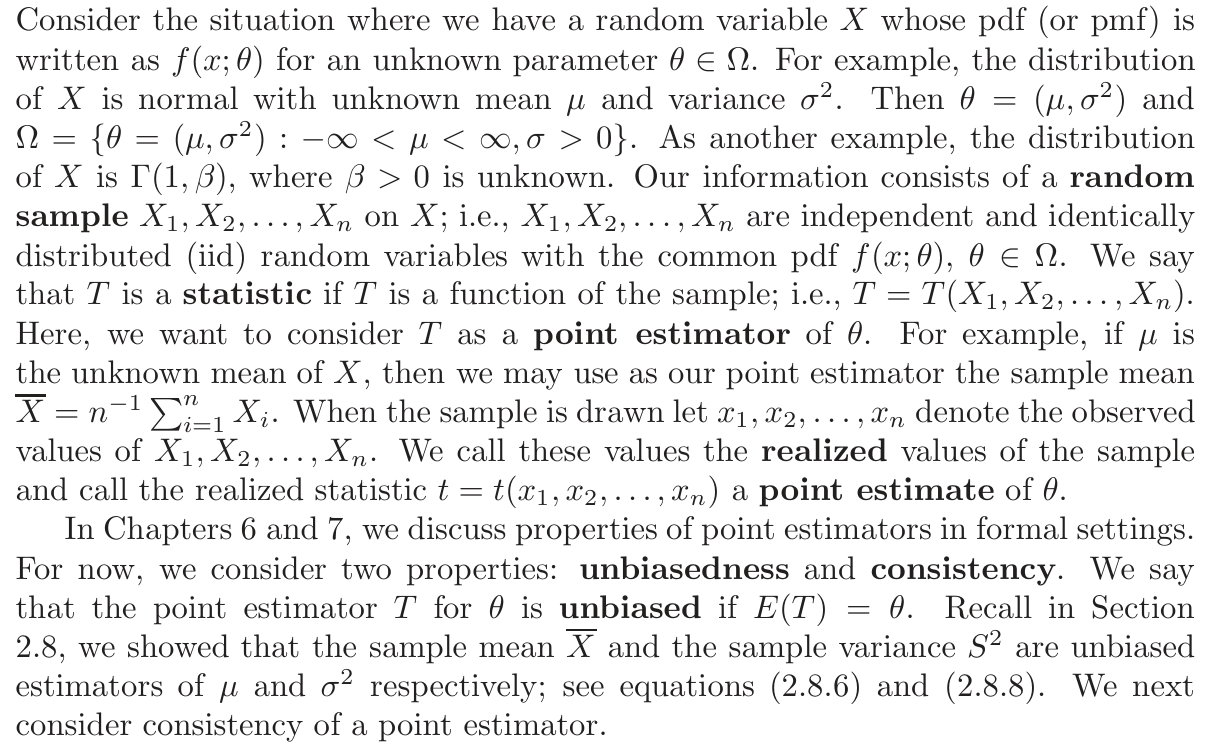
\includegraphics[width=\textwidth]{2-chap5-20250309.png}
% \caption{}
\label{}
\end{figure}

\begin{figure}[H]
\centering
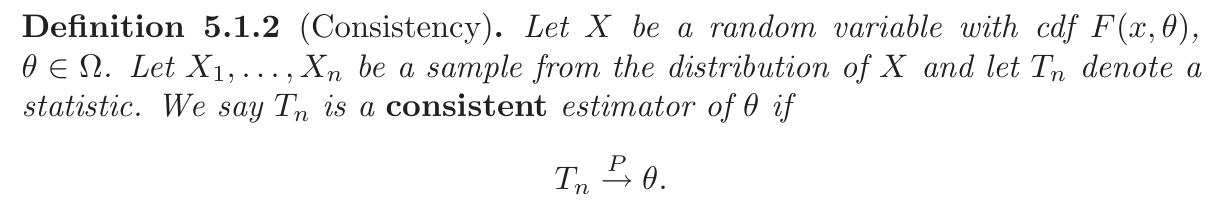
\includegraphics[width=\textwidth]{3-chap5-20250309.png}
% \caption{}
\label{}
\end{figure}

\subsection{Convergence in Distribution}

In many situations we can show statistic convergence without the distribution function of the statistic. But how close is the statistic to the estimator?

\begin{figure}[H]
\centering
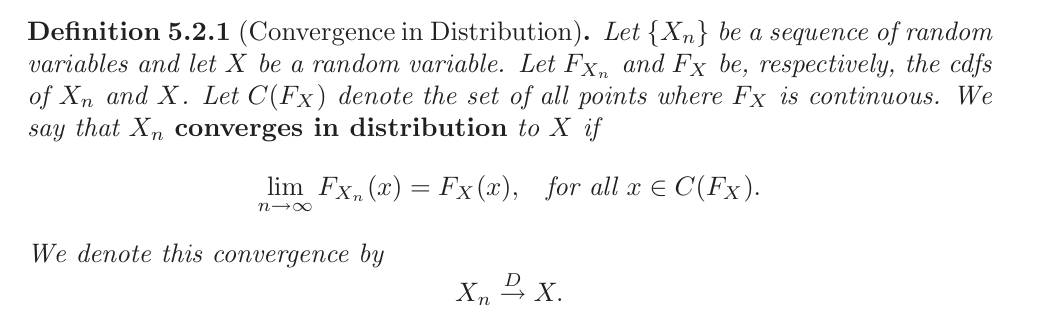
\includegraphics[width=\textwidth]{4-chap5-20250309.png}
% \caption{}
\label{}
\end{figure}

\begin{figure}[H]
\centering
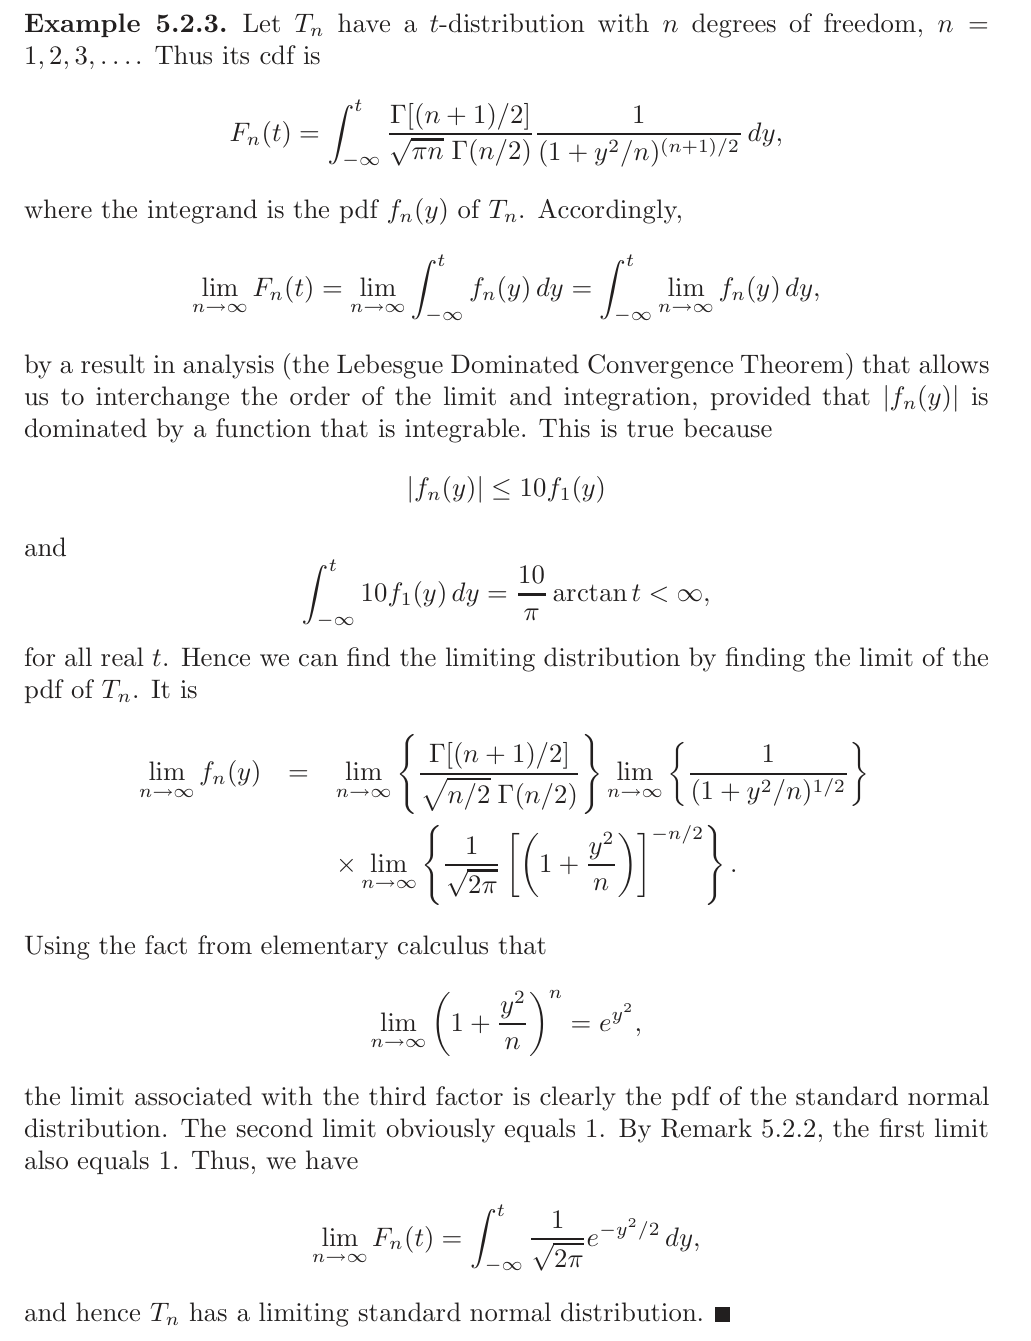
\includegraphics[width=\textwidth]{5-chap5-20250309.png}
% \caption{}
\label{}
\end{figure}

\begin{theorem}[Stirling's formula]
\[
\Gamma(k+1)\sim \sqrt{ 2\pi }k^{k+1/2 }e^{ -k }
\]
\end{theorem}
\begin{figure}[H]
\centering
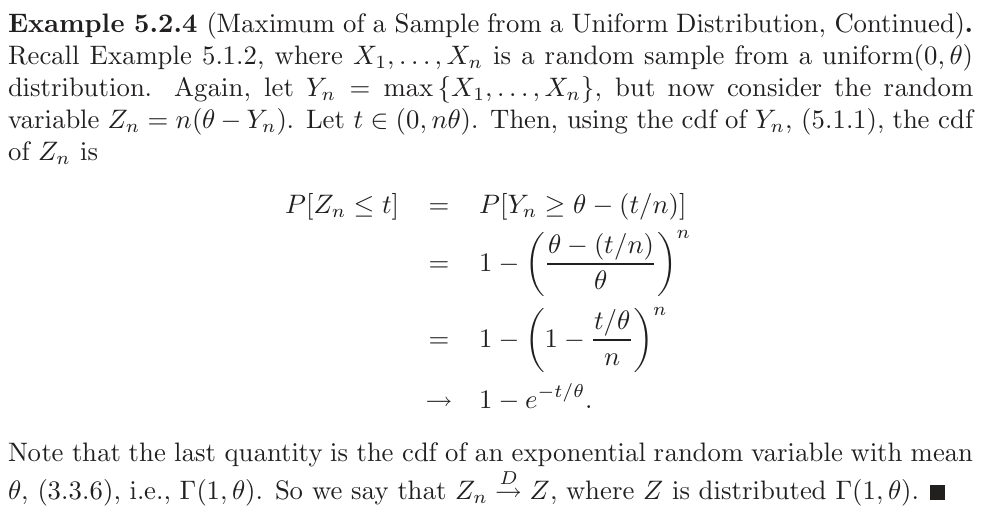
\includegraphics[width=\textwidth]{6-chap5-20250309.png}
% \caption{}
\label{}
\end{figure}

Convergence in distribution is weaker than convergence in probability. Thus convergence in distribution is often called weak convergence.

\begin{theorem}
If $X_n$ converges to $X$ in probability, then $X_n$ converges to $X$ in distribution.\label{4b6469}
\end{theorem}\begin{proof}
Let $x$ be a point of continuity of $F_{X}(x)$. For every $\epsilon>0$,
\[
\begin{aligned}
F_{X_n}(x) & =P[X_n\leq x] \\
 & =P[\{ X_n\leq x \}\cap \{ \lvert X_n-X \rvert <\epsilon \}]+P[\{ X_n\leq x \}\cap \{ \lvert X_n-X \rvert \geq \epsilon \}] \\
 & \leq P[X\leq x+\epsilon]+P[\lvert X_n-X \rvert \geq \epsilon]
\end{aligned}
\]
Basd on this inequality and the fact that $X_n\overset{ P }{ \to }X$ we see that
\[
\limsup_{ n \to \infty } F_{X_n}(x)\leq F_{X}(x+\epsilon)
\]
To get a lower bound, we proceed similarly with the complement to show that
\[
P[X_n>x]\leq P[X\geq x-\epsilon]+P[\lvert X_n-X \rvert \geq \epsilon]
\]
Hence
\[
\liminf_{ n \to \infty } F_{X_n}(x)\geq F_{X}(x-\epsilon)
\]
Using a relationship between $\limsup$ and $\liminf$, it follows that
\[
F_{X}(x-\epsilon)\leq \liminf_{ n \to \infty } F_{X_n}(x)\leq \limsup_{ n \to \infty } F_{X_n}(x)\leq F_{X}(x+\epsilon)
\]
Letting $\epsilon \downarrow0$ gives us the desired result.
\end{proof}

\begin{figure}[H]
\centering
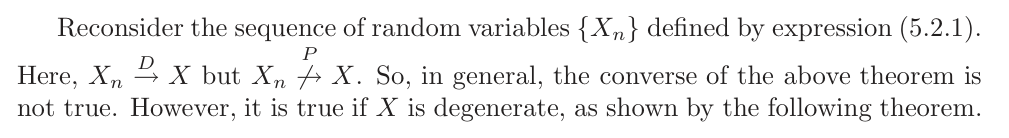
\includegraphics[width=\textwidth]{7-chap5-20250309.png}
% \caption{}
\label{}
\end{figure}

\begin{figure}[H]
\centering
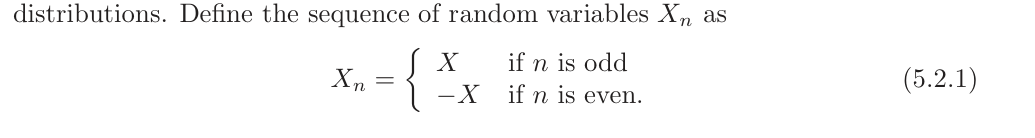
\includegraphics[width=\textwidth]{9-chap5-20250309.png}
% \caption{}
\label{}
\end{figure}

\begin{theorem}
If $X_n\overset{ D }{ \to }b$ constant, then $X_n\overset{ P }{ \to }b$.
\end{theorem}
Let $\epsilon>0$ be given. Then
\[
\lim_{ n \to \infty } P[\lvert X_n-b \rvert \leq \epsilon]=\lim_{ n \to \infty } F_{X_n}(b+\epsilon)-\lim_{ n \to \infty } F_{X_n}[(b-\epsilon)-0]=1-0=1
\]
The converse is not true.

\begin{theorem}
$X_n\overset{ D }{ \to }X,Y_n\overset{ P }{ \to }0$ then $X_n+Y_n\overset{ D }{ \to }X$.\label{e41498}
\end{theorem}

The proof is similar to the above theorem.

We often use this result as follows. Suppose it is difficult to show that $X_n$ converges to $X$ in distributino, but it is easy to show that $Y_n$ converges in distribution to $X$ and that $X_n-Y_n$ converges to 0 in probability. Hence by this last theorem. $X_n=Y_n+(X_n-Y_n)\overset{ D }{ \to }X$ as desired.

The next two theorems state general results.

\begin{theorem}
$X_n\overset{ D }{ \to }X$ and $g$ continuous on the support of $X$. Then $g(X_n)\overset{ D }{ \to }g(X)$.\label{721da5}
\end{theorem}

An often-used application of this theorem occurs when we have a sequence of random variables $Z_n$ which converges in distribution to a standard normal random variable $Z$. Because the distribution of $Z^{2}$ is $\chi^{2}(1)$, it follows by the above theorem that $Z_n^{2}$ converges in distribution to a $\chi^{2}(1)$ distribution.

\begin{theorem}[Slutsky's theorem]
If $X_n\overset{ D }{ \to }X,A_n\overset{ P }{ \to }a$ and $B_n\overset{ P }{ \to }b$ then $A_n+B_nX_n\overset{ D }{ \to }a+bX$.\label{1136a4}
\end{theorem}

The proof is similar to \cref{4b6469}

\subsection{Bounded in Probability}

\begin{figure}[H]
\centering
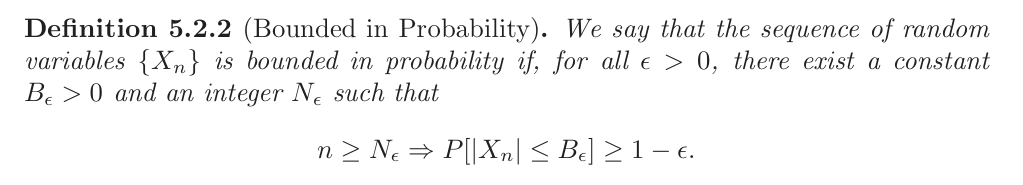
\includegraphics[width=\textwidth]{10-chap5-20250309.png}
% \caption{}
\label{}
\end{figure}

\begin{theorem}
\begin{figure}[H]
\centering
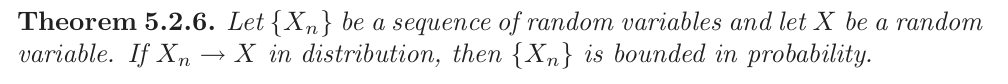
\includegraphics[width=\textwidth]{11-chap5-20250309.png}
% \caption{}
\label{}
\end{figure}\label{b809d0}
\end{theorem}

One way of thinking of a sequence that is bounded in probability (or one that is converging to a random variable in distribution) is that the probability mass of $\lvert X_n \rvert$ is not escaping to $\infty$. At times we can use boundedness in probability instead of convergence in distribution. A property we will need  later is given in the following theorem:

\begin{theorem}
Let $\{ X_n \}$ be a sequence of random variables bounded in probability and let $\{ Y_n \}$ be a sequence of random variables that converges to 0 in probability. Then
\[
X_nY_n\overset{ P }{ \to }0
\]
\end{theorem}
Let $\epsilon>0$ is given. Choose $B_{\epsilon}>0$ and an integer $N_{\epsilon}$ such that
\[
n\geq N_{\epsilon}\Rightarrow P[\lvert X_n \rvert \leq B_{\epsilon}]\geq 1-\epsilon
\]
Then
\[
\varlimsup_{ n \to \infty } P[\lvert X_nY_n \rvert \geq \epsilon]\leq \varlimsup_{ n \to \infty } P[\lvert X_nY_n \rvert \geq \epsilon,\lvert X_n \rvert \leq B_{\epsilon}]+\varlimsup_{ n \to \infty } P[\lvert X_nY_n \rvert \geq \epsilon,\lvert X_n \rvert >B_{\epsilon}]\leq \varlimsup_{ n \to \infty } P[\lvert Y_n \rvert \geq \epsilon/B_{\epsilon}]+\epsilon=\epsilon
\]
\begin{remark}
It's similar to $X_n,Y_n\overset{ P }{ \to }X,Y\Rightarrow X_nY_n\overset{ P }{ \to }XY$.
\end{remark}
\subsection{\texorpdfstring{$\Delta$}{Delta}-Method}

The $\Delta$-method is employed to determine the asymptotic distribution of a function of a random variable, given the distribution of the random variable itself. This is analogous to problems discussed in previous chapters, such as \cref{721da5} and \cref{1136a4}.

\textbf{Little-o Notation}

The notation $Y_n=o_p(X_n)$ signifies that $Y_n$ converges to 0 in probability relative to $X_n$, formally:
\[
Y_n=o_p(X_n) \text { if and only if } \frac{Y_n}{X_n} \xrightarrow{P} 0 \text {, as } n \rightarrow \infty.
\]
\textbf{Big-O Notation}

The notation $Y_n=O_p(X_n)$ indicates that $\frac{Y_n}{X_n}$ is bounded in probability as $n \rightarrow \infty$.

\begin{theorem}[Theorem 5.2.8.]
If $\{Y_n\}$ is a sequence of random variables that is bounded in probability and $X_n=o_p(Y_n)$, then $X_n \xrightarrow{P} 0$ as $n \rightarrow \infty$.\label{cf8d09}
\end{theorem}

\textbf{Proof of Theorem 5.2.8}

Let $\epsilon>0$. Then, there exist $N_{\epsilon}$ and $B_{\epsilon}$ such that for $n \geq N_{\epsilon}$, $P[|Y_n| \leq B_{\epsilon}] \geq 1-\epsilon$. Since $\frac{X_n}{Y_n} \xrightarrow{P} 0$, we have:
\[
P[|X_n| \geq \epsilon]=P[|X_n| \geq \epsilon,|Y_n| \leq B_{\epsilon}]+P[|X_n| \geq \epsilon,|Y_n| >B_{\epsilon}]\leq P\left[ \frac{X_n}{| Y_n |}\geq \frac{\epsilon}{B_{\epsilon}} \right]+P[| Y_n | >B_{\epsilon}]\to\epsilon
\]
\begin{theorem}[Theorem 5.2.9 ($\Delta$-Method)]
Let $\{X_n\}$ be a sequence of random variables such that
\[
\sqrt{n}(X_n-\theta) \xrightarrow{D} N(0, \sigma^2).
\]If $g(x)$ is differentiable at $\theta$ and $g^{\prime}(\theta) \neq 0$, then
\[
\sqrt{n}(g(X_n)-g(\theta)) \xrightarrow{D} N(0, \sigma^2(g^{\prime}(\theta))^2).
\]
\end{theorem}
\textbf{Proof of Theorem 5.2.9}

Since $g(X_n)=g(\theta)+g'(\theta)(X_n-\theta)+o_{p}(|X_n-\theta |)$, it follows that
\[
\sqrt{ n }(g(X_n)-g(\theta))=g'(\theta)\sqrt{ n }(X_n-\theta)+o_{p}(\sqrt{ n }|X_n-\theta |)
\]
Because $\sqrt{ n }(X_n-\theta)\overset{ D }{ \to }N(0,\sigma^{2})$, it implies that $\sqrt{ n }|X_n-\theta |$ is bounded in probability. Therefore, by \cref{cf8d09} , $o_{p}(\sqrt{ n }|X_n-\theta |)\to0$ in probability. Hence, the result follows.

\subsection{Moment Generating Function Technique}

It's difficult to obtain $\lim_{ n \to \infty }F_{X_n}(x)$, but quite easier from the mgf $M_n$ that corresponds to the cdf $F_{X_n}(x)$.

\begin{figure}[H]
\centering
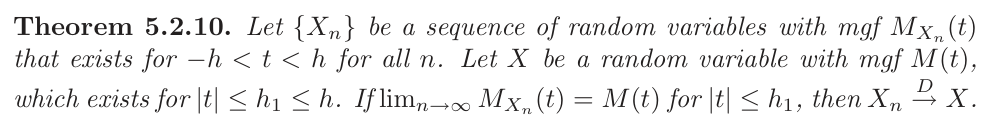
\includegraphics[width=\textwidth]{15-chap5-20250309.png}
% \caption{}
\label{}
\end{figure}

\begin{figure}[H]
\centering
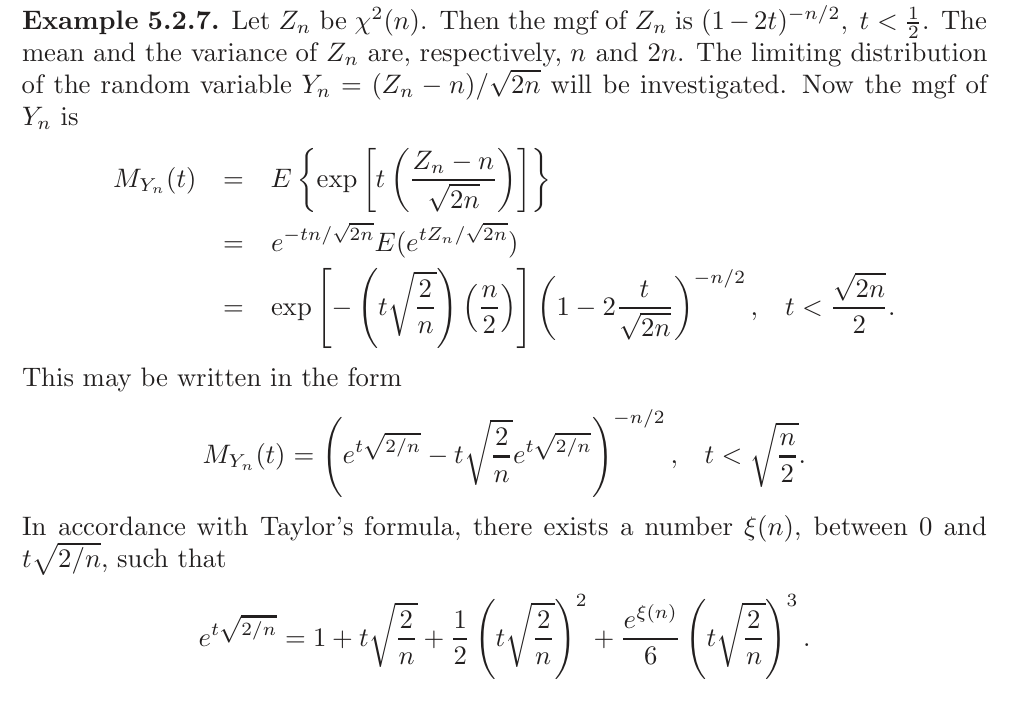
\includegraphics[width=\textwidth]{16-chap5-20250309.png}
% \caption{}
\label{}
\end{figure}

\begin{figure}[H]
\centering
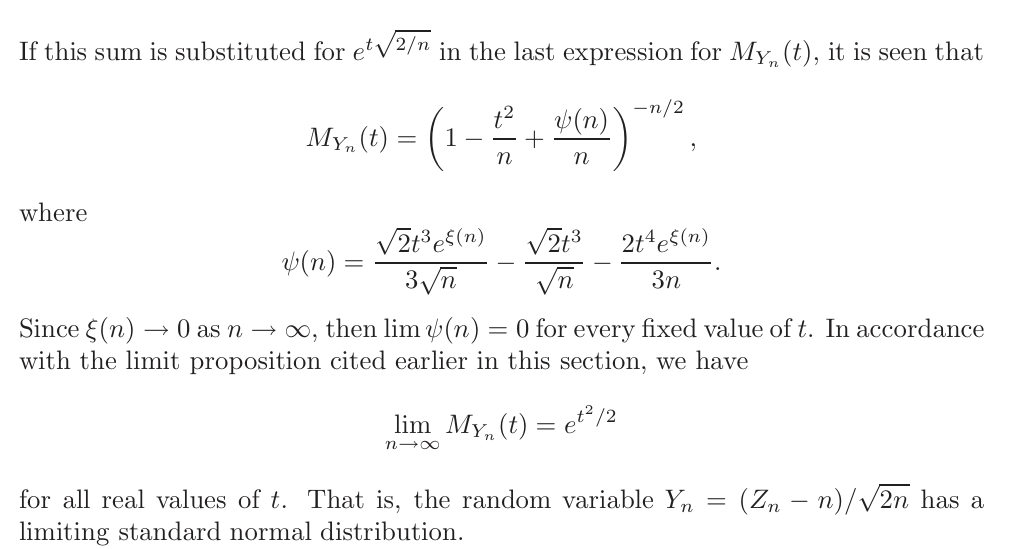
\includegraphics[width=\textwidth]{17-chap5-20250309.png}
% \caption{}
\label{}
\end{figure}

\subsection{Central Limit Theorem}

\begin{figure}[H]
\centering
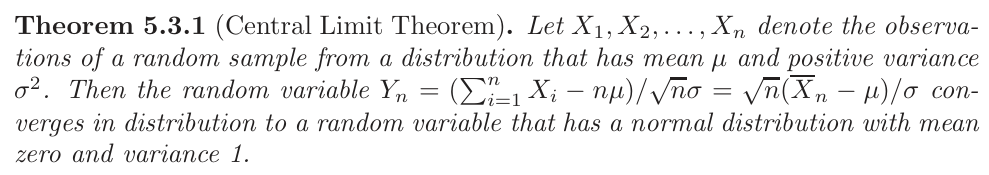
\includegraphics[width=\textwidth]{18-chap5-20250309.png}
% \caption{}
\label{}
\end{figure}

Prove by characteristic function $\varphi(t)=E(e^{ itX })$.

The Central Limit Theorem is saying that when $n$ is large, fixed positive integer, the random variable $\overline{X}$ has an approximate normal distribution with mean $\mu$ and variance $\sigma^{2}/n$. We can equivalently state the conclusion of the Central Limit Theorem as
\[
\sqrt{ n }(\overline{X}-\mu)\overset{ \mathcal{D} }{ \to }N(0,\sigma^{2})
\]
This is often a convenient formulation to use.

\begin{remark}
We know that $\overline{X}$ and $\sum_{i=1}^{n}X_i$ have approximately normal distributions, provided that $n$ is large enough. Later, we find that other statistics also have approximate normal distributions, and this is the reason that the normal distribution is so improtant to statisticians. That is, while not many underlying distributions are normal, the distributions of statistics calculated from random samples arising from these distributions are often close to being normal.
\end{remark}
We can combine $\Delta$ -method with Central Limit Theorem. Assume that $X_1,\dots,X_n$ is a random sample on $X$ which has finite mean $\mu$ and variance $\sigma^{2}$. Then by the Central Limit Theorem, we have
\[
\sqrt{ n }(\overline{X}-\mu)\overset{ \mathcal{D} }{ \to }N(0,\sigma^{2})
\]
Hence by the $\Delta$ -method, we have
\[
\sqrt{ n }[g(\overline{X})-g(\mu)]\overset{ \mathcal{D} }{ \to }N(0,\sigma^{2}(g'(\mu))^{2})
\]
for a continuous transformation $g(x)$ such that $g'(\mu)\neq0$.

\subsection{Extensions to Multivariate Distributions}

This section discusses asymptotic concepts for sequences of random vectors.

\begin{definition}[convergence in probability]
Let $\{\mathbf{X}_n\}$ be a sequence of $p$-dimensional random vectors, and let $\mathbf{X}$ be a random vector, all defined on the same sample space. We say that $\{\mathbf{X}_n\}$ \textbf{converges in probability} to $\mathbf{X}$ if
\[
\lim_{n \rightarrow \infty} P\left[\left\|\mathbf{X}_n-\mathbf{X}\right\| \geq \epsilon\right]=0
\]for all $\epsilon>0$. As in the univariate case, we write $\mathbf{X}_n \xrightarrow{P} \mathbf{X}$.
\end{definition}
\begin{theorem}[Theorem 5.4.1]
Let $\{\mathbf{X}_n\}$ be a sequence of $p$-dimensional random vectors, and let $\mathbf{X}$ be a random vector, all defined on the same sample space. Then $\mathbf{X}_n \xrightarrow{P} \mathbf{X}$ if and only if $X_{n j} \xrightarrow{P} X_j$ for all $j=1, \ldots, p$.\label{479de5}
\end{theorem}

Based on \cref{479de5}, many theorems involving convergence in probability can be extended to the multivariate setting.

Let $\{ \mathbf{X}_n \}$ be a sequence of i.i.d. random vectors with common mean vector $\boldsymbol{\mu}$ and variance-covariance matrix $\boldsymbol{\Sigma}$. Denote the vector of means by $\mathbf{\overline{X}}_n=\frac{1}{n}\sum_{i=1}^{n}\mathbf{X}_i$. By the Weak Law of Large Numbers, $\overline{X}_j\to \mu _j$ in probability for each $j$. Hence, by \cref{479de5}, $\overline{\mathbf{X}}_n\to \boldsymbol{\mu}$ in probability.

Now consider the analog of the sample variances. Let $\mathbf{X}_i=(X_{i1},\dots,X_{ip})'$. Define the sample variances and covariances by
\[
S_{n,jj}=S_{n,j}^{2}=\frac{1}{n-1}\sum_{i=1}^{n} (X_{ij}-\overline{X}_j)^{2}\quad \text{for }j=1,\dots,p
\]
\[
S_{n,jk}=\frac{1}{n-1}\sum_{i=1}^{n} (X_{ij}-\overline{X}_j)(X_{ik}-\overline{X}_k)\quad \text{for }j\neq k=1,\dots,p
\]
If we define the $p\times p$ matrix $\mathbf{S}=(S_{n,jk})$, then $\mathbf{S}\to\boldsymbol{\Sigma}$ in probability.

\begin{definition}[convergence in distribution]
Let $\{\mathbf{X}_n\}$ be a sequence of random vectors with $\mathbf{X}_n$ having distribution function $F_n(\mathbf{x})$, and let $\mathbf{X}$ be a random vector with distribution function $F(\mathbf{x})$. Then $\{\mathbf{X}_n\}$ \textbf{converges in distribution} to $\mathbf{X}$ if
\[
\lim_{n\rightarrow \infty}F_n(\mathbf{x})=F(\mathbf{x}),
\]for all points $\mathbf{x}$ at which $F(\mathbf{x})$ is continuous. We write $\mathbf{X}_n \xrightarrow{D} \mathbf{X}$.
\end{definition}
\begin{theorem}
Let $\{\mathbf{X}_n\}$ be a sequence of random vectors that converges in distribution to a random vector $\mathbf{X}$, and let $g(\mathbf{x})$ be a function that is continuous on the support of $\mathbf{X}$. Then $g(\mathbf{X}_n)$ converges in distribution to $g(\mathbf{X})$.
\end{theorem}
\begin{theorem}
Let $\{\mathbf{X}_n\}$ be a sequence of random vectors with $\mathbf{X}_n$ having distribution function $F_n(\mathbf{x})$ and moment generating function $M_n(\mathbf{t})$. Let $\mathbf{X}$ be a random vector with distribution function $F(\mathbf{x})$ and moment generating function $M(\mathbf{t})$. Then $\{\mathbf{X}_n\}$ converges in distribution to $\mathbf{X}$ if and only if, for some $h>0$,
\[
\lim_{n\rightarrow \infty}M_n(\mathbf{t})=M(\mathbf{t}),
\]for all $\mathbf{t}$ such that $\|\mathbf{t}\|<h$.
\end{theorem}
\begin{theorem}[Multivariate Central Limit Theorem]
Let $\{\mathbf{X}_n\}$ be a sequence of i.i.d. random vectors with common mean vector $\boldsymbol{\mu}$ and variance-covariance matrix $\boldsymbol{\Sigma}$ which is positive definite. Assume that the common moment generating function $M(\mathbf{t})$ exists in an open neighborhood of $\mathbf{0}$. Let
\[
\mathbf{Y}_n=\frac{1}{\sqrt{n}} \sum_{i=1}^n\left(\mathbf{X}_i-\boldsymbol{\mu}\right)=\sqrt{n}(\overline{\mathbf{X}}-\boldsymbol{\mu})
\]Then $\mathbf{Y}_n$ converges in distribution to a $N_p(\mathbf{0}, \boldsymbol{\Sigma})$ distribution.
\end{theorem}
\textbackslash{}begin\{proof\}
Let $\mathbf{t}\in \mathbf{R}^{p}$ be a vector in the stipulated neighborhood of $\mathbf{0}$. The moment generating function of $\mathbf{Y}_n$ is
\[
M_n(\mathbf{t})=\mathbb{E}\left[ \exp \left\{  \mathbf{t}'\frac{1}{\sqrt{ n }} \sum_{i=1}^{n} (\mathbf{X}_i-\boldsymbol{\mu})  \right\} \right]=\mathbb{E}\left[ \exp \left\{  \frac{1}{\sqrt{ n }} \sum_{i=1}^{n} \mathbf{t}'(\mathbf{X}_i-\boldsymbol{\mu})  \right\} \right]=\mathbb{E}\left[ \exp \left\{  \frac{1}{\sqrt{ n }} \sum_{i=1}^{n} W_i  \right\} \right]
\]
where $W_i=\mathbf{t}'(\mathbf{X}_i-\boldsymbol{\mu})$. Note that $W_i$ are i.i.d. with mean 0 and variance $\mathrm{Var}(W_i)=\mathbf{t}'\boldsymbol{\Sigma}\mathbf{t}$. Hence, by the standard Central Limit Theorem,
\[
\frac{1}{\sqrt{ n }}\sum_{i=1}^{n} W_i\overset{ D }{ \to }N(0,\mathbf{t}'\boldsymbol{\Sigma}\mathbf{t})
\]
Then $M_n(\mathbf{t})$ is the MGF of $(1/\sqrt{ n })\sum_{i=1}^{n}W_i$ evaluated at 1. Therefore, we must have
\[
M_n(\mathbf{t})=\mathbb{E}\left[ \exp \left\{  1\cdot \frac{1}{\sqrt{ n }} \sum_{i=1}^{n} W_i  \right\} \right]\to e^{ 1^{2}\mathbf{t}'\boldsymbol{\Sigma}\mathbf{t}/2 }=e^{ \mathbf{t}'\boldsymbol{\Sigma}\mathbf{t}/2 }.
\]
Because the last quantity is the moment generating function of a $N_{p}(\mathbf{0},\boldsymbol{\Sigma})$ distribution, the result follows.
\textbackslash{}end\{proof\}

\begin{theorem}[Theorem 5.4.5]
Let $\{\mathbf{X}_n\}$ be a sequence of $p$-dimensional random vectors. Suppose $\mathbf{X}_n \xrightarrow{D} N(\boldsymbol{\mu}, \boldsymbol{\Sigma})$. Let $\mathbf{A}$ be an $m \times p$ matrix of constants, and let $\mathbf{b}$ be an $m$-dimensional vector of constants. Then $\mathbf{A} \mathbf{X}_n+\mathbf{b} \xrightarrow{D} N\left(\mathbf{A} \boldsymbol{\mu}+\mathbf{b}, \mathbf{A} \boldsymbol{\Sigma} \mathbf{A}^{\prime}\right)$.
\end{theorem}
\begin{theorem}[Theorem 5.4.6]
Let $\{\mathbf{X}_n\}$ be a sequence of $p$-dimensional random vectors. Suppose
\[
\sqrt{n}\left(\mathbf{X}_n-\boldsymbol{\mu}_0\right) \xrightarrow{D} N_p(\mathbf{0}, \boldsymbol{\Sigma}) .
\]Let $\mathbf{g}$ be a transformation $\mathbf{g}(\mathbf{x})=\left(g_1(\mathbf{x}), \ldots, g_k(\mathbf{x})\right)^{\prime}$ such that $1 \leq k \leq p$ and the $k \times p$ matrix of partial derivatives,
\[
\mathbf{B}=\left[\frac{\partial g_i}{\partial \mu_j}\right], \quad i=1, \ldots k ; j=1, \ldots, p
\]are continuous and do not vanish in a neighborhood of $\boldsymbol{\mu}_0$. Let $\mathbf{B}_0=\mathbf{B}$ at $\boldsymbol{\mu}_0$. Then
\[
\sqrt{n}\left(\mathbf{g}\left(\mathbf{X}_n\right)-\mathbf{g}\left(\boldsymbol{\mu}_0\right)\right) \xrightarrow{D} N_k\left(\mathbf{0}, \mathbf{B}_0 \boldsymbol{\Sigma} \mathbf{B}_0^{\prime}\right) .
\]
\end{theorem}
% \section{常见分布}

\begin{itemize}
    \item \textbf{二项分布 (Binomial Distribution)}
    \begin{itemize}
        \item 记作:$X \sim B(n, p)$
        \item PMF:$$P(X = k) = \binom{n}{k} p^k (1-p)^{n-k}, \quad k = 0, 1, \ldots, n$$
        \item MGF:$$M_X(t) = (1-p+pe^t)^n$$
        \item 特征函数:$$\varphi_X(t) = (1-p+pe^{it})^n$$
    \end{itemize}

    \item \textbf{负二项分布 (Negative Binomial Distribution)}
    \begin{itemize}
        \item 记作:$X \sim NB(r, p)$
        \item PMF:$$P(X = k) = \binom{k+r-1}{k} p^r (1-p)^k, \quad k = 0, 1, 2, \ldots$$
        \item MGF:$$M_X(t) = \left(\frac{p}{1-(1-p)e^t}\right)^r, \quad t < -\ln(1-p)$$
        \item 特征函数:$$\varphi_X(t) = \left(\frac{p}{1-(1-p)e^{it}}\right)^r$$
    \end{itemize}

    \item \textbf{几何分布 (Geometric Distribution)}
    \begin{itemize}
        \item 记作:$X \sim Geo(p)$
        \item PMF:$$P(X = k) = p(1-p)^{k-1}, \quad k = 1, 2, \ldots$$
        \item MGF:$$M_X(t) = \frac{pe^t}{1-(1-p)e^t}, \quad t < -\ln(1-p)$$
        \item 特征函数:$$\varphi_X(t) = \frac{pe^{it}}{1-(1-p)e^{it}}$$
    \end{itemize}

    \item \textbf{多项分布 (Multinomial Distribution)}
    \begin{itemize}
        \item 记作:$\mathbf{X} \sim Mult(n, \mathbf{p})$,其中 $\mathbf{p} = (p_1, p_2, \ldots, p_k)$
        \item PMF:$$P(\mathbf{X} = \mathbf{x}) = \frac{n!}{x_1! x_2! \cdots x_k!} p_1^{x_1} p_2^{x_2} \cdots p_k^{x_k}$$,其中 $\sum_{i=1}^k x_i = n$
        \item MGF:$$M_{\mathbf{X}}(\mathbf{t}) = (p_1 e^{t_1} + p_2 e^{t_2} + \cdots + p_k e^{t_k})^n$$
        \item 特征函数:$$\varphi_{\mathbf{X}}(\mathbf{t}) = (p_1 e^{it_1} + p_2 e^{it_2} + \cdots + p_k e^{it_k})^n$$
    \end{itemize}

    \item \textbf{超几何分布 (Hypergeometric Distribution)}
    \begin{itemize}
        \item 记作:$X \sim HGeom(N, K, n)$
        \item PMF:$$P(X = k) = \frac{\binom{K}{k} \binom{N-K}{n-k}}{\binom{N}{n}}, \quad \max(0, n+K-N) \leq k \leq \min(n, K)$$
        \item MGF:无简单表达式
        \item 特征函数:无简单表达式
    \end{itemize}

    \item \textbf{泊松分布 (Poisson Distribution)}
    \begin{itemize}
        \item 记作:$X \sim Pois(\lambda)$
        \item PMF:$$P(X = k) = \frac{\lambda^k e^{-\lambda}}{k!}, \quad k = 0, 1, 2, \ldots$$
        \item MGF:$$M_X(t) = e^{\lambda(e^t-1)}$$
        \item 特征函数:$$\varphi_X(t) = e^{\lambda(e^{it}-1)}$$
    \end{itemize}

    \item \textbf{伽马分布 (Gamma Distribution)}
    \begin{itemize}
        \item 记作:$X \sim Gamma(\alpha, \beta)$
        \item PDF:$$f(x) = \frac{\beta^\alpha}{\Gamma(\alpha)} x^{\alpha-1} e^{-\beta x}, \quad x > 0$$
        \item CDF:$F(x) = \frac{\gamma(\alpha, \beta x)}{\Gamma(\alpha)}, \quad x > 0$,其中 $\gamma(\alpha, y)$ 是不完全伽马函数
        \item MGF:$$M_X(t) = \left(1-\frac{t}{\beta}\right)^{-\alpha}, \quad t < \beta$$
        \item 特征函数:$$\varphi_X(t) = \left(1-\frac{it}{\beta}\right)^{-\alpha}$$
    \end{itemize}

    \item \textbf{卡方分布 (Chi-Square Distribution)}
    \begin{itemize}
        \item 记作:$X \sim \chi^2(k)$,是自由度为 $k$ 的卡方分布
        \item PDF:$$f(x) = \frac{1}{2^{k/2}\Gamma(k/2)} x^{k/2-1} e^{-x/2}, \quad x > 0$$
        \item CDF:$F(x) = \frac{\gamma(k/2, x/2)}{\Gamma(k/2)}, \quad x > 0$
        \item MGF:$$M_X(t) = (1-2t)^{-k/2}, \quad t < 1/2$$
        \item 特征函数:$$\varphi_X(t) = (1-2it)^{-k/2}$$
    \end{itemize}

    \item \textbf{贝塔分布 (Beta Distribution)}
    \begin{itemize}
        \item 记作:$X \sim Beta(\alpha, \beta)$
        \item PDF:$$f(x) = \frac{1}{B(\alpha, \beta)} x^{\alpha-1} (1-x)^{\beta-1}, \quad 0 < x < 1$$
        \item CDF:$F(x) = \frac{B_x(\alpha, \beta)}{B(\alpha, \beta)}, \quad 0 \leq x \leq 1$,其中 $B_x(\alpha, \beta)$ 是不完全贝塔函数
        \item MGF:无简单表达式
        \item 特征函数:无简单表达式
    \end{itemize}

    \item \textbf{正态分布 (Normal Distribution)}
    \begin{itemize}
        \item 记作:$X \sim N(\mu, \sigma^2)$
        \item PDF:$$f(x) = \frac{1}{\sqrt{2\pi\sigma^2}} e^{-\frac{(x-\mu)^2}{2\sigma^2}}, \quad x \in \mathbb{R}$$
        \item CDF:$F(x) = \Phi\left(\frac{x-\mu}{\sigma}\right) = \frac{1}{2}\left[1 + \text{erf}\left(\frac{x-\mu}{\sigma\sqrt{2}}\right)\right]$
        \item MGF:$$M_X(t) = e^{\mu t + \frac{1}{2}\sigma^2 t^2}$$
        \item 特征函数:$$\varphi_X(t) = e^{i\mu t - \frac{1}{2}\sigma^2 t^2}$$
    \end{itemize}

    \item \textbf{t 分布 (Student's t-Distribution)}
    \begin{itemize}
        \item 记作:$X \sim t(n)$,其中 $n$ 是自由度
        \item PDF:$$f(x) = \frac{\Gamma(\frac{n+1}{2})}{\sqrt{n\pi}\Gamma(\frac{n}{2})}\left(1+\frac{x^2}{n}\right)^{-\frac{n+1}{2}}, \quad x \in \mathbb{R}$$
        \item CDF:无简单表达式
        \item MGF:不存在
        \item 特征函数:无简单表达式
    \end{itemize}

    \item \textbf{F 分布 (F-Distribution)}
    \begin{itemize}
        \item 记作:$X \sim F(d_1, d_2)$,其中 $d_1, d_2$ 是自由度
        \item PDF:$$g_1(w)=\frac{\Gamma\left[\left(r_1+r_2\right) / 2\right]\left(r_1 / r_2\right)^{r_1 / 2}}{\Gamma\left(r_1 / 2\right) \Gamma\left(r_2 / 2\right)} \frac{w^{r_1 / 2-1}}{\left(1+r_1 w / r_2\right)^{\left(r_1+r_2\right) / 2}} \quad 0<w<\infty$$
        \item CDF:无简单表达式
        \item MGF:不存在
        \item 特征函数:无简单表达式
    \end{itemize}
\end{itemize}

\section{The standard machine: approximate Borel function by simple functions}

If we want to verify a property that holds for general Borel-measurable function $f$, we can follow four steps as below.

\begin{itemize}
	\item Verify the property when $f$ is indicator function.
	\item Verify the property when $f$ is nonnegative simple function.
	\item Verify the property when $f$ is Borel-measurable function
	\item Verify the property when $f$ is General Borel-measurable function
\end{itemize}

An example is as follow.

\subsection{Example}

\begin{theorem}
Let $X$ be a random variable on a probability space $(\Omega,\mathcal{F},\mathbb{P})$ and let $g$ be a Borel-measurable function on $\mathbb{R}$. Then
\[
\mathbb{E}\lvert g(X) \rvert =\int_{\mathbb{R}}^{} \lvert g(x) \rvert  \, d\mu_{X}(x) 
\]
and if this quantity is finite, then
\[
\mathbb{E}g(X)=\int_{\mathbb{R}}^{} g(x) \, d\mu_{X}(x) 
\]
\end{theorem}
\begin{proof}
Step 1. Indicator functions. (Omitted)

Step 2. Nonnegative simple functions. (Trivial because of the linearity)

Step 3. Nonnegative Borel-measurable functions. Let $g(x)$ be an arbitraty nonnegative Borel-measurable function defined on $\mathbb{R}$. For each positive integer $n$, define the sets
\[
B_{k,n}=\left\{  x;\frac{k}{2^{n}} \leq g(x)<\frac{k+1}{2^{n}}  \right\},\qquad k=0,1,2,\dots,4^{n}-1
\]
\begin{remark}
这样的定义是为了保证在 $n\to \infty$ 时,每个划分越来越细,同时 $\bigcup_{k=1}^{4^{n}-1}B_{k,n}\to[0,+\infty)$. 而且对于任意 $n$,$\{ B_{k,n+1} \}$ 是 $\{ B_{k,n} \}$ 的加细($B_{k,n}$ 的划分点都包含在 $B_{k,n+1}$ 的划分点集内)
\end{remark}
For eac fixed $n$, the sets $B_{0,n},B_{1,n},\dots,B_{4^{n}-1,n}$ correspond to the partition
\[
0<\frac{1}{2^{n}}<\frac{2}{2^{n}}<\dots<\frac{4^{n}}{2^{n}}=2^{n}.
\]
At the next stage $n+1$, the partition points include all those at stage $n$ and new partition points at the midpoints between te old ones. Because of this fact, the simple functions
\[
g_n(x)=\sum_{k=0}^{4^{n}-1} \frac{k}{2^{n}}\mathbb{I}_{B_{k,n}}(x)
\]
satisfy $0\leq g_1\leq g_2\leq\dots\leq g$. Furthermore, these functions become more and more accurate approximations of $g$ as $n$ becomes larger; indeed $\lim_{ n \to \infty }g_n(x)=g(x)$ for every $x\in \mathbb{R}$. From Step 2, we knoe that
\[
\mathbb{E}g_n(X)=\int_{\mathbb{R}}^{} g_n(x) \, d\mu_{X}(x)
\]
for every $n$. Letting $n\to \infty$ and using the Monotone Convergence Theorem, on both sides of the equation, we obtain
\[
\mathbb{E}g(X)=\lim_{ n \to \infty } \mathbb{E}g_n(X)=\lim_{ n \to \infty } \int_{\mathbb{R}}^{} g_n(x) \, d\mu_{X}(x)=\int_{\mathbb{R}}^{} g(x) \, d\mu_{X}(x)
\]
This proves when $g$ is a nonnegative Borel-measurable function.

Step 4. General Borel-measurable function. (consider $g=g^{+}-g^{-}$ where $g^{+}$ and $g^{-}$ are both nonnegative Borel-measurable functions)

\end{proof}

\input{../数理统计/includes/Convergence-of-Random-Variables.tex}
\input{../数理统计/includes/Models-Statistical-Inference-and-Learning.tex}
\input{../数理统计/includes/Bootstrap.tex}
\input{../数理统计/includes/Parametric-Inference.tex}

\section{第一次作业}
\begin{figure}[H]
\centering
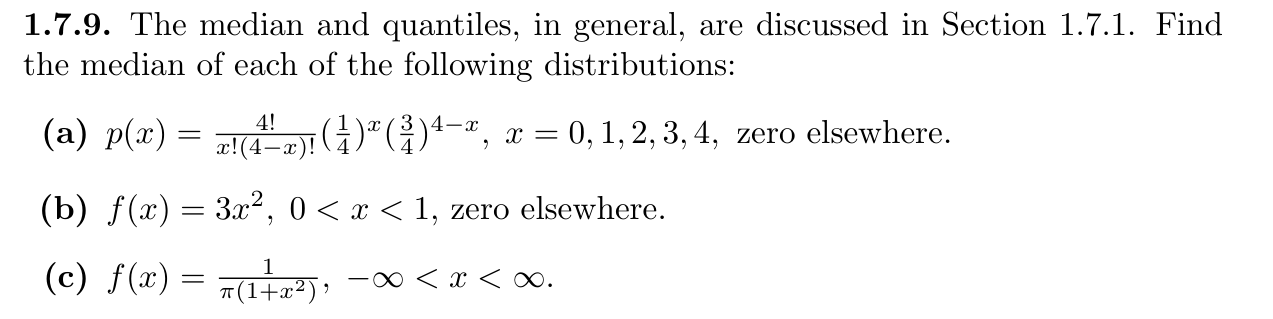
\includegraphics[width=\textwidth]{hw1-20250302.png}
% \caption{}
\label{}
\end{figure}
(a)
\[
\begin{aligned}
p(0) & =\left( \frac{3}{4} \right)^{4}=0.316406 \\
p(1) & =\left( \frac{3}{4} \right)^{3}=0.421875
\end{aligned}
\]
Then $p(x<1)\leq0.5,p(x\leq1)\geq0.5$, $\,1$ is the median. Or say that $\xi_{1/2 }\in(0,1]$.
(b)
\[
F(x)=\int_{0}^{x} 3t^{2} \, dt =t^{3}\qquad x\in(0,1)
\]
Then $\xi_{1/2 }=F^{-1}\left( \frac{1}{2} \right)=\sqrt[3]{ \frac{1}{2} }$ .
(c)
\[
F(x)=\int_{-\infty}^{x} \frac{1}{\pi(1+t^{2})}  \, dt =\frac{1}{2}+\frac{\arctan x}{\pi}
\]
Then $\xi_{1/2 }=F^{-1}\left( \frac{1}{2} \right)=0$.

\begin{figure}[H]
\centering
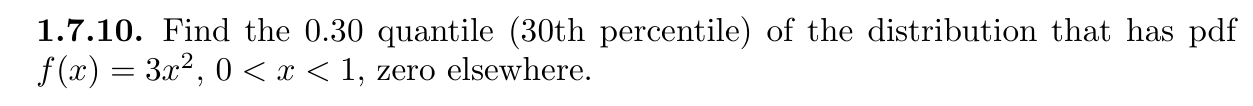
\includegraphics[width=\textwidth]{1-hw1-20250302.png}
% \caption{}
\label{}
\end{figure}
\[
F(x)=\int_{0}^{x} 3t^{2} \, dt =x^{3}\qquad x\in(0,1)
\]
Then $\xi_{0.3}=F^{-1}(0.3)=\sqrt[3]{ 0.3 }$.

\begin{figure}[H]
\centering
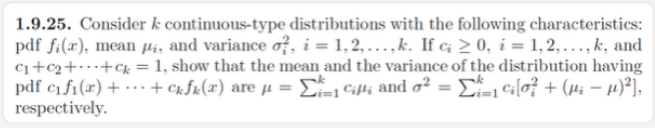
\includegraphics[width=\textwidth]{hw1-20250304.png}
% \caption{}
\label{}
\end{figure}
\[
\mu=\int_{-\infty}^{\infty} x\cdot\sum_{i=1}^{k} c_if_i(x) \, dx =\sum_{i=1}^{k} c_i\int_{-\infty}^{\infty} x\cdot f_i(x) \, dx =\sum_{i=1}^{k} c_{i}\mu _i
\]
\[
\begin{aligned}
\sigma^{2} & =\int_{-\infty}^{\infty} (x-\mu)^{2} \sum_{i=1}^{k} c_if_i(x)\, dx  \\
 & =\sum_{i=1}^{k} c_i\int_{-\infty}^{\infty} x^{2}f_i(x) \, dx -2\mu \cdot \sum_{i=1}^{k}  c_i\int_{-\infty}^{\infty} xf_i(x) \, dx +\mu^{2} \sum_{i=1}^{k} c_i\int_{-\infty}^{\infty} f_i(x) \, dx  \\
 & =\sum_{i=1}^{k} c_i\sigma _i^{2}-2\mu \cdot \sum_{i=1}^{k} c_i \mu _i +\mu^{2}\sum_{i=1}^{k} c_i \\
 & =\sum_{i=1}^{k} c_i[\sigma _i^{2}+(\mu _i-\mu)^{2}] 
\end{aligned}
\]
\begin{figure}[H]
\centering
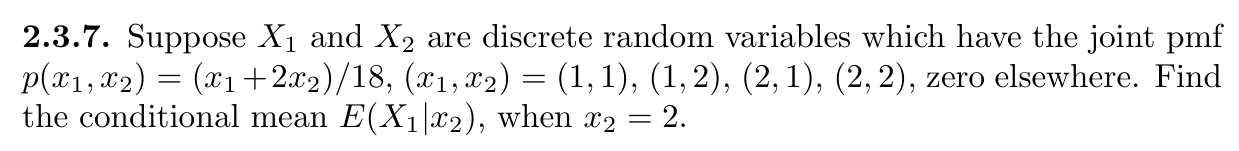
\includegraphics[width=\textwidth]{2-hw1-20250302.png}
% \caption{}
\label{}
\end{figure}
\[
\begin{aligned}
\left.E(X_{1}|x_{2})\right|_{x_{2}=2} & =\sum_{x_{1}}x_{1}\cdot \left.p_{1|2}(x_{1},x_{2})\right|_{x_{2}=2}=\sum_{x_{1}}x_{1}\cdot \left.\frac{p(x_1,x_2)}{p_2(x_2)}\right|_{x_{2}=2} \\
 & =\frac{1\cdot p(1,2)+2\cdot p(2,2)}{p(1,2)+p(2,2)}=\frac{\frac{5}{18}+2\cdot\frac{6}{18}  }{\frac{5}{18}+\frac{6}{18}  }=\frac{17}{11} 
\end{aligned}
\]
\begin{figure}[H]
\centering
\includegraphics[width=\textwidth]{3-hw1-20250302.png}
% \caption{}
\label{}
\end{figure}
\[
\begin{aligned}
E(Y|x) & =\int_{-\infty}^{\infty} y\cdot f_{Y|X}(x,y) \, dy =\int_{-\infty}^{\infty} y\cdot\frac{f(x,y)}{f_{X}(x)} \, dy=\int_{-\infty}^{\infty} y\cdot\frac{3\exp \{ -x-2y \}\mathbb{1}_{0<y<x<\infty}}{\int_{-\infty}^{\infty} 3\exp \{ -x-2y \}\mathbb{1}_{0<y<x<\infty} \, dy } \, dy  \\
 & =\int_{0}^{x} y\cdot\frac{\exp \{ -x-2y \}}{\int_{0}^{x} \exp \{ -x-2y \} \, dy } \, dy=\int_{0}^{x} y \cdot\frac{e^{ -x-2y }}{e^{ -x }(1-e^{ -2x })/2}\, dy=\frac{2}{1-e^{ -2x }}\int_{0}^{x} y\cdot e^{ -2y } \, dy  \\
 & =\frac{e^{ 2x }-2x-1}{2(e^{ 2x }-1)} \end{aligned} 
\]
\begin{figure}[H]
\centering
\includegraphics[width=\textwidth]{4-hw1-20250302.png}
% \caption{}
\label{}
\end{figure}

Characteristic function $\phi(t)=M(it)=\left( \frac{1}{3}+\frac{2}{3}e^{ it } \right)^{2}=\frac{1}{9}+\frac{4}{9}e^{ it }+\frac{4}{9}e^{ 2it }$, by the inverse formula
\[
f(x)=\frac{1}{2\pi}\int_{-\infty}^{\infty} e^{ -itx }\phi (t)  \, dt=\frac{1}{2\pi}\int_{-\infty}^{\infty} \frac{1}{9}e^{ -itx }+\frac{4}{9}e^{ -it(x-1) }+\frac{4}{9}e^{ -it(x-2) } \, dt = \frac{1}{9}\delta_0+\frac{4}{9}\delta_1+\frac{4}{9}\delta_2
\]
Then $X_1$ is discrete random variable with $P(X_1=0)=\frac{1}{9},P(X_1=1)=\frac{4}{9},P(X_1=2)=\frac{4}{9}$.
The mgf of $Y=X_1+X_2+X_3$ is
\[
M_{Y}(t)=E(e^{ t(X_1+X_2+X_3) })\overset{ iid }{ = }E(e^{ tX_1 })E(e^{ tX_2 })E(e^{ tX_3 })=\left( \frac{1}{3}+\frac{2}{3}e^{ t } \right)^{6}
\]
\begin{table}[h]
	\centering
	\begin{tabular}{|c|c|c|c|c|c|c|c|}
		\hline
		$Y$ & 0 & 1 & 2 & 3 & 4 & 5 & 6 \\
		\hline
		$P$ & $\frac{1}{729}$ & $\frac{4}{243}$ & $\frac{20}{243}$ & $\frac{160}{729}$ & $\frac{80}{243}$ & $\frac{64}{243}$ & $\frac{64}{729}$ \\
		\hline
	\end{tabular}
\end{table}
\section{第二次作业}
\begin{lstlisting}
5.1 7 9
5.2 7 18
5.3 11 12
\end{lstlisting}
\begin{figure}[H]
\centering
\includegraphics[width=\textwidth]{hw3-20250313.png}
% \caption{}
\label{}
\end{figure}

For
\[
\begin{aligned}
F_{Y_n}(y) & =P(Y_n\leq y)=1-P(Y_n>y)=1-P(\min\{ X_1,\dots,X_n \}>y) \\
 & =1-P(X_i>y;i=1,2,\dots,n)=1-\prod_{i=1}^{n} (1-P(X_i\leq y)) \\
 & =1-\prod_{i=1}^{n} (1-F_{X_i}(y))
\end{aligned}
\]
If $y\leq\theta$ then $F_{X_i}(y)=\int_{-\infty}^{y} f(x) \, dx=0$ thus $F_{Y_n}(y)=1-\prod_{i=1}^{n}(1-0)=0$.
If $y>\theta$ then
\[
F_{Y_n}(y)=1-\prod_{i=1}^{n} \left( 1-\int_{\theta}^{y} e^{ -(x-\theta) } \, dx  \right)=1-\prod_{i=1}^{n} e^{ -(y-\theta) }=1-e^{ -n(y-\theta) }
\]
Then for any $\varepsilon>0$, we have
\[
P(\lvert Y_n-\theta \rvert \leq \varepsilon)=P(\theta-\varepsilon \leq Y_n\leq \theta+\varepsilon)=F_{Y_n}(\theta+\varepsilon)-F_{Y_n}(\theta-\varepsilon-0)=F_{Y_n}(\theta+\varepsilon)=1-e^{ -n\varepsilon }
\]
Therefore $\lim_{ n \to \infty }P(\lvert Y_n-\theta \rvert \leq\varepsilon)=\lim_{ n \to \infty }(1-e^{ -n\varepsilon })=1$, i.e. $Y_n\to\theta$ in probability.

\begin{figure}[H]
\centering
\includegraphics[width=\textwidth]{1-hw3-20250313.png}
% \caption{}
\label{}
\end{figure}
\[
p_{Y_n}(y)=F'_{Y_n}(y)=\begin{cases}
ne^{ -n(y-\theta) } & y>\theta \\
0 & y\leq \theta
\end{cases}
\]
\[
E(Y_n)=\int_{-\infty}^{\infty} yp_{Y_n}(y) \, dy =\int_{-\infty}^{\infty} y\cdot ne^{ -n(y-\theta) }\mathbb{1_{(\theta,+\infty)}}(y)  \, dy=\int_{\theta}^{+\infty } y\cdot ne^{ -n(y-\theta) } \, dy =n\theta+1
\]
Since $E(Y_n)\neq\theta$, $Y_n$ is not an unbiased estimator of $\theta$. But $Z_n=\frac{Y_n-1}{n}$ has the mean $\theta$ thus is an unbiased estimator of $\theta$.

\begin{figure}[H]
\centering
\includegraphics[width=\textwidth]{2-hw3-20250313.png}
% \caption{}
\label{}
\end{figure}

To assure the existence, we use the characteristic functions.
\[
\varphi_{X_n}(t)=E(e^{ iX_nt })=\left( 1-\frac{it}{\beta} \right)^{-n}
\]
\[
\begin{aligned}
\varphi_{Y_n}(t) & =E(e^{ iY_nt })=E(e^{ iX_nt/n  })=\varphi_{X_n}(t/n )=\left( 1-\frac{it}{n\beta} \right)^{-n} \\
 & =\exp \left\{  -n\log\left( 1-\frac{it}{n\beta} \right)  \right\}=\exp \left\{  \frac{it}{\beta}+o(1)  \right\} \\
 & \to e^{ it/\beta } \qquad \text{as }n\to \infty
\end{aligned}
\]
Denote $Y=\lim_{ n \to \infty }Y_n$.
By the inverse formula
\[
p_{Y}(x)=\frac{1}{2\pi} \int_{-\infty}^{\infty} e^{ it/\beta }\cdot e^{ -itx } \, dt=\delta_{1/\beta}(x)
\]
Then
\[
F_{Y}(x)=\begin{cases}
0 & x\leq \frac{1}{\beta} \\
1 & x> \frac{1}{\beta}  
\end{cases}
\]
\begin{figure}[H]
\centering
\includegraphics[width=\textwidth]{3-hw3-20250313.png}
% \caption{}
\label{}
\end{figure}
\[
\begin{aligned}
M_{Y_n}(t) & =E(e^{t \sqrt{ n }(\overline{X_n}-1) })=e^{ -t\sqrt{ n } }E\left( e^{t \frac{X_1+\dots+X_n}{\sqrt{ n }} } \right) =e^{ -t\sqrt{ n } }\prod_{k=1}^{n} E(e^{ tX_k/\sqrt{ n } }) \\
 & =e^{ -t\sqrt{ n } }\prod_{k=1}^{n} \int_{0}^{\infty} e^{ tx/\sqrt{ n } }e^{ -x } \, dx =e^{ -\sqrt{ n } }\left( \frac{1}{1-\frac{t}{\sqrt{ n }} }  \right)^{n} \\
 & =\exp \left\{  -t\sqrt{ n }-n\log\left( 1-\frac{t}{\sqrt{ n }}  \right)  \right\} \\
 & =\exp \{ -t\sqrt{ n }+t\sqrt{ n }+t^{2}/2+o(n^{-1/2 })\} \\
 & \to e^{ t^{2}/2 }\qquad \text{as }n\to \infty
\end{aligned}
\]
Denote $Y=\lim_{ n \to \infty }Y_n$, then
\[
\begin{aligned}
p_{Y}(x) & =\frac{1}{2\pi}\int_{-\infty}^{\infty} e^{ itx }M_{Y}(it) \, dt =\frac{1}{2\pi}\int_{-\infty}^{\infty} e^{ itx }e^{ -t^{2}/2  } \, dt  \\
 & =\frac{1}{2\pi}\int_{-\infty}^{\infty} e^{ -(t-ix)^{2}/2  }e^{ -x^{2}/2 } \, dt=\frac{1}{\sqrt{ 2\pi }}e^{ -x^{2}/2 }
\end{aligned}
\]
Thus $Y\sim N(0,1)$, which means
\[
Y_n=\sqrt{ n }(\overline{X}_n-1)\overset{ \mathcal{D} }{ \to }N(0,1)
\]
Let $g(x)\coloneqq \sqrt{ x }$, using the $\Delta$ -method, we have
\[
\sqrt{ n }(\sqrt{ \overline{X}_n }-\sqrt{ 1 })=\sqrt{ n }(g(\overline{X}_n)-g(1))\overset{ \mathcal{D} }{ \to }N(0,1\cdot(g'(1))^{2})=N\left( 0,\frac{1}{4} \right)
\]
Therefore the limiting distribution of $\sqrt{ n }(\sqrt{ \overline{X_n} }-1)$ is $N\left( 0,\frac{1}{4} \right)$.
\begin{figure}[H]
\centering
\includegraphics[width=\textwidth]{4-hw3-20250313.png}
% \caption{}
\label{}
\end{figure}

We know that
\[
\sqrt{ n }(\overline{X}-\mu)\overset{ \mathcal{D} }{ \to }N(0,\sigma^{2})
\]
Let $u(x)=x^{3}$ then $u'(x)=3x^{2}$. Using the $\Delta$ -method, we have
\[
\sqrt{ n }(u(\overline{X})-u(\mu))\overset{ \mathcal{D} }{ \to }N(0,\sigma^{2}(u'(\mu))^{2})=N(0,9\sigma^{2}\mu^{4})
\]
Therefore
\[
u(\overline{X})\overset{ \mathcal{D} }{ \to }N(\mu^{3},9\sigma^{2}\mu^{4}/n)
\]
\begin{figure}[H]
\centering
\includegraphics[width=\textwidth]{5-hw3-20250313.png}
% \caption{}
\label{}
\end{figure}

We know that
\[
\sqrt{ n }(\overline{X}-\mu)\overset{ \mathcal{D} }{ \to }N(0,\mu)
\]
Let $u(x)=\sqrt{ x }$ then $u'(x)=\frac{1}{2\sqrt{ x }}$. Using the $\Delta$ -method, we have
\[
\sqrt{ n }(u(\overline{X})-u(\mu))\overset{ \mathcal{D} }{ \to }N(0,\mu \cdot(u'(\mu))^{2})=N\left( 0,\frac{1}{4} \right)
\]
Therefore
\[
u(\overline{X})\overset{ \mathcal{D} }{ \to }N\left( \sqrt{ \mu },\frac{1}{4n}  \right)
\]
which means the variance of $\sqrt{ \frac{Y}{n} }$ is essentially free of $\mu$.

\section{第三次作业}
\begin{lstlisting}
5.1 7 9
5.2 7 18
5.3 11 12
\end{lstlisting}
\begin{figure}[H]
\centering
\includegraphics[width=\textwidth]{hw3-20250313.png}
% \caption{}
\label{}
\end{figure}

For
\[
\begin{aligned}
F_{Y_n}(y) & =P(Y_n\leq y)=1-P(Y_n>y)=1-P(\min\{ X_1,\dots,X_n \}>y) \\
 & =1-P(X_i>y;i=1,2,\dots,n)=1-\prod_{i=1}^{n} (1-P(X_i\leq y)) \\
 & =1-\prod_{i=1}^{n} (1-F_{X_i}(y))
\end{aligned}
\]
If $y\leq\theta$ then $F_{X_i}(y)=\int_{-\infty}^{y} f(x) \, dx=0$ thus $F_{Y_n}(y)=1-\prod_{i=1}^{n}(1-0)=0$.
If $y>\theta$ then
\[
F_{Y_n}(y)=1-\prod_{i=1}^{n} \left( 1-\int_{\theta}^{y} e^{ -(x-\theta) } \, dx  \right)=1-\prod_{i=1}^{n} e^{ -(y-\theta) }=1-e^{ -n(y-\theta) }
\]
Then for any $\varepsilon>0$, we have
\[
P(\lvert Y_n-\theta \rvert \leq \varepsilon)=P(\theta-\varepsilon \leq Y_n\leq \theta+\varepsilon)=F_{Y_n}(\theta+\varepsilon)-F_{Y_n}(\theta-\varepsilon-0)=F_{Y_n}(\theta+\varepsilon)=1-e^{ -n\varepsilon }
\]
Therefore $\lim_{ n \to \infty }P(\lvert Y_n-\theta \rvert \leq\varepsilon)=\lim_{ n \to \infty }(1-e^{ -n\varepsilon })=1$, i.e. $Y_n\to\theta$ in probability.

\begin{figure}[H]
\centering
\includegraphics[width=\textwidth]{1-hw3-20250313.png}
% \caption{}
\label{}
\end{figure}
\[
p_{Y_n}(y)=F'_{Y_n}(y)=\begin{cases}
ne^{ -n(y-\theta) } & y>\theta \\
0 & y\leq \theta
\end{cases}
\]
\[
E(Y_n)=\int_{-\infty}^{\infty} yp_{Y_n}(y) \, dy =\int_{-\infty}^{\infty} y\cdot ne^{ -n(y-\theta) }\mathbb{1_{(\theta,+\infty)}}(y)  \, dy=\int_{\theta}^{+\infty } y\cdot ne^{ -n(y-\theta) } \, dy =n\theta+1
\]
Since $E(Y_n)\neq\theta$, $Y_n$ is not an unbiased estimator of $\theta$. But $Z_n=\frac{Y_n-1}{n}$ has the mean $\theta$ thus is an unbiased estimator of $\theta$.

\begin{figure}[H]
\centering
\includegraphics[width=\textwidth]{2-hw3-20250313.png}
% \caption{}
\label{}
\end{figure}

To assure the existence, we use the characteristic functions.
\[
\varphi_{X_n}(t)=E(e^{ iX_nt })=\left( 1-\frac{it}{\beta} \right)^{-n}
\]
\[
\begin{aligned}
\varphi_{Y_n}(t) & =E(e^{ iY_nt })=E(e^{ iX_nt/n  })=\varphi_{X_n}(t/n )=\left( 1-\frac{it}{n\beta} \right)^{-n} \\
 & =\exp \left\{  -n\log\left( 1-\frac{it}{n\beta} \right)  \right\}=\exp \left\{  \frac{it}{\beta}+o(1)  \right\} \\
 & \to e^{ it/\beta } \qquad \text{as }n\to \infty
\end{aligned}
\]
Denote $Y=\lim_{ n \to \infty }Y_n$.
By the inverse formula
\[
p_{Y}(x)=\frac{1}{2\pi} \int_{-\infty}^{\infty} e^{ it/\beta }\cdot e^{ -itx } \, dt=\delta_{1/\beta}(x)
\]
Then
\[
F_{Y}(x)=\begin{cases}
0 & x\leq \frac{1}{\beta} \\
1 & x> \frac{1}{\beta}  
\end{cases}
\]
\begin{figure}[H]
\centering
\includegraphics[width=\textwidth]{3-hw3-20250313.png}
% \caption{}
\label{}
\end{figure}
\[
\begin{aligned}
M_{Y_n}(t) & =E(e^{t \sqrt{ n }(\overline{X_n}-1) })=e^{ -t\sqrt{ n } }E\left( e^{t \frac{X_1+\dots+X_n}{\sqrt{ n }} } \right) =e^{ -t\sqrt{ n } }\prod_{k=1}^{n} E(e^{ tX_k/\sqrt{ n } }) \\
 & =e^{ -t\sqrt{ n } }\prod_{k=1}^{n} \int_{0}^{\infty} e^{ tx/\sqrt{ n } }e^{ -x } \, dx =e^{ -\sqrt{ n } }\left( \frac{1}{1-\frac{t}{\sqrt{ n }} }  \right)^{n} \\
 & =\exp \left\{  -t\sqrt{ n }-n\log\left( 1-\frac{t}{\sqrt{ n }}  \right)  \right\} \\
 & =\exp \{ -t\sqrt{ n }+t\sqrt{ n }+t^{2}/2+o(n^{-1/2 })\} \\
 & \to e^{ t^{2}/2 }\qquad \text{as }n\to \infty
\end{aligned}
\]
Denote $Y=\lim_{ n \to \infty }Y_n$, then
\[
\begin{aligned}
p_{Y}(x) & =\frac{1}{2\pi}\int_{-\infty}^{\infty} e^{ itx }M_{Y}(it) \, dt =\frac{1}{2\pi}\int_{-\infty}^{\infty} e^{ itx }e^{ -t^{2}/2  } \, dt  \\
 & =\frac{1}{2\pi}\int_{-\infty}^{\infty} e^{ -(t-ix)^{2}/2  }e^{ -x^{2}/2 } \, dt=\frac{1}{\sqrt{ 2\pi }}e^{ -x^{2}/2 }
\end{aligned}
\]
Thus $Y\sim N(0,1)$, which means
\[
Y_n=\sqrt{ n }(\overline{X}_n-1)\overset{ \mathcal{D} }{ \to }N(0,1)
\]
Let $g(x)\coloneqq \sqrt{ x }$, using the $\Delta$ -method, we have
\[
\sqrt{ n }(\sqrt{ \overline{X}_n }-\sqrt{ 1 })=\sqrt{ n }(g(\overline{X}_n)-g(1))\overset{ \mathcal{D} }{ \to }N(0,1\cdot(g'(1))^{2})=N\left( 0,\frac{1}{4} \right)
\]
Therefore the limiting distribution of $\sqrt{ n }(\sqrt{ \overline{X_n} }-1)$ is $N\left( 0,\frac{1}{4} \right)$.
\begin{figure}[H]
\centering
\includegraphics[width=\textwidth]{4-hw3-20250313.png}
% \caption{}
\label{}
\end{figure}

We know that
\[
\sqrt{ n }(\overline{X}-\mu)\overset{ \mathcal{D} }{ \to }N(0,\sigma^{2})
\]
Let $u(x)=x^{3}$ then $u'(x)=3x^{2}$. Using the $\Delta$ -method, we have
\[
\sqrt{ n }(u(\overline{X})-u(\mu))\overset{ \mathcal{D} }{ \to }N(0,\sigma^{2}(u'(\mu))^{2})=N(0,9\sigma^{2}\mu^{4})
\]
Therefore
\[
u(\overline{X})\overset{ \mathcal{D} }{ \to }N(\mu^{3},9\sigma^{2}\mu^{4}/n)
\]
\begin{figure}[H]
\centering
\includegraphics[width=\textwidth]{5-hw3-20250313.png}
% \caption{}
\label{}
\end{figure}

We know that
\[
\sqrt{ n }(\overline{X}-\mu)\overset{ \mathcal{D} }{ \to }N(0,\mu)
\]
Let $u(x)=\sqrt{ x }$ then $u'(x)=\frac{1}{2\sqrt{ x }}$. Using the $\Delta$ -method, we have
\[
\sqrt{ n }(u(\overline{X})-u(\mu))\overset{ \mathcal{D} }{ \to }N(0,\mu \cdot(u'(\mu))^{2})=N\left( 0,\frac{1}{4} \right)
\]
Therefore
\[
u(\overline{X})\overset{ \mathcal{D} }{ \to }N\left( \sqrt{ \mu },\frac{1}{4n}  \right)
\]
which means the variance of $\sqrt{ \frac{Y}{n} }$ is essentially free of $\mu$.

\section{第四次作业}
\begin{lstlisting}
•    Section 4.1: 2, 6, 8  
•    Section 4.2: 3, 9, 10
\end{lstlisting}
\begin{figure}[H]
\centering
\includegraphics[width=\textwidth]{hw4-20250321.png}
% \caption{}
\label{}
\end{figure}

(a)
\begin{figure}[H]
\centering
\includegraphics[width=\textwidth]{Figure_1.png}
% \caption{}
\label{}
\end{figure}
The normal probability model is credible.

(b)
For normal distributions, the mles are
\[
\widehat{\mu}=\overline{X}=201
\]
\[
\widehat{\sigma }^{2}=n^{-1}\sum_{i=1}^{n} (X_i-\overline{X})^{2}=293.923
\]
\[
\widehat{\sigma}=\sqrt{ 293.923 }\approx17.145
\]
\[
\widehat{(\mu/\sigma)}=\widehat{\mu}/\widehat{\sigma}\approx11.723
\]
Locate $\widehat{\mu}$ on the plot:
\begin{figure}[H]
\centering
\includegraphics[width=\textwidth]{Figure_1 1.png}
% \caption{}
\label{}
\end{figure}

Overlay the normal pdf with these estimates:
\begin{figure}[H]
\centering
\includegraphics[width=\textwidth]{Figure_1 2.png}
% \caption{}
\label{}
\end{figure}

(c)
\[
L(p)={\binom{n}{X} }p^{X}(1-p)^{n-X}
\]
where $X$ is the number of successes (pitchers weighing over 215 pounds) and $p$ is the probability of success (a pitcher weighing over 215 pounds).
\[
\begin{aligned}
\frac{dL(p)}{dp} & ={\binom{n}{X} }(Xp^{X-1}(1-p)^{n-X}-p^{X}(n-X)(1-p)^{n-X-1}) \\
 & ={\binom{n}{X} }p^{X-1}(1-p)^{n-X-1}(X(1-p)-(n-X)p) \\
 & ={\binom{n}{X} }p^{X-1}(1-p)^{n-X-1}(X-np)
\end{aligned}
\]
Let $\frac{dL(p)}{dp}=0$ then
\[
\widehat{p}=\frac{X}{n}=\frac{7}{26}
\]
(d)
\[
p=P(X>215)=1-\Phi\left( \frac{215-\mu}{\sigma} \right)
\]
where $\Phi$ is the CDF of the standard normal distribution $N(0,1)$. Then
\[
\widehat{p}=1-\Phi\left( \frac{215-\widehat{\mu}}{\widehat{\sigma}} \right)\approx0.207
\]
\begin{figure}[H]
\centering
\includegraphics[width=\textwidth]{1-hw4-20250321.png}
% \caption{}
\label{}
\end{figure}

The estimator
\[
\widehat{p}(a_j)=\frac{1}{n}\sum_{i=1}^{n} I_j(X_i)
\]
where
\[
I_j(X_i)=\begin{cases}
1 & X_i=a_j \\
0 & X_i\neq a_j.
\end{cases}
\]
Its variance is
\[
\begin{aligned}
\mathrm{Var}(\widehat{p}(a_j)) & =E[\widehat{p}(a_j)^{2}]-(E[\widehat{p}(a_j)])^{2} \\
 & =E\left[ \left( \frac{1}{n}\sum_{i=1}^{n} I_j(X_i) \right)^{2} \right]-p(a_j)^{2} \\
 & =\frac{1}{n^{2}}\sum_{i,k=1}^{n} E[I_j(X_i)I_j(X_k)]-p(a_j)^{2} \\
 & =\frac{2}{n^{2}}\sum_{1\leq i<k\leq n}\underbrace{ E[I_j(X_i)I_j(X_k)] }_{ =E[I_j(X_i)]E[I_j(X_k)] }+\frac{1}{n^{2}}\cdot n\sum_{i=1}^{n} E[I^{2}_j(X_i)]-p(a_j)^{2} \\
 & =\frac{1}{n^{2}}n(n-1) p(a_j)^{2}+\frac{1}{n}p(a_j)-p(a_j)^{2} \\
 & =\frac{1}{n}(p(a_j)-p(a_j)^{2})
\end{aligned}
\]
Its mgf is
\[
\begin{aligned}
M(t) & =E[e^{ \widehat{p}(a_j)t }]=E\left[ \exp \left\{  \frac{1}{n}\sum_{i=1}^{n} I_j(X_i)t  \right\} \right] \\
 & =\prod_{i=1}^{n} E\left[ \exp \left\{  I_j(X_i)\frac{t}{n}  \right\} \right]   \\
 & =\prod_{i=1}^{n} \left( 1-p(a_j)+p(a_j)e^{ \frac{t}{n} } \right) \\
 & =(1+p(a_j)(e^{ \frac{t}{n} }-1))^{n}
\end{aligned}
\]
\begin{figure}[H]
\centering
\includegraphics[width=\textwidth]{2-hw4-20250321.png}
% \caption{}
\label{}
\end{figure}

For Poisson distribution with mean $\lambda$, we have
\[
P(X=k)=\frac{\lambda^{k}e^{ -\lambda }}{k!},\qquad k=0,1,2,\dots
\]
The likelihood function is
\[
l(\lambda)=\sum_{i=1}^{n} \log\frac{\lambda^{x_i}e^{ -\lambda }}{x_i!}=-n\lambda+(\log\lambda)\cdot \sum_{i=1}^{n} x_i-\sum_{i=1}^{n} \log (x_i!)
\]
The first parital of the log-likelihood with respect to $\lambda$ is
\[
\frac{ \partial l(\lambda) }{ \partial \lambda } =-n+\frac{1}{\lambda}\sum_{i=1}^{n} x_i
\]
Setting this partial to 0 and solving for $\lambda$, we obtain the solution $\frac{1}{n}\sum_{i=1}^{n}x_i$, thus the mle of $\lambda$ is
\[
\widehat{\lambda}=\frac{1}{n}\sum_{i=1}^{n} X_i=\overline{X}=\frac{64}{30}\approx2.133
\]
The mle of the pmf is
\[
P(X=j)=\frac{\widehat{\lambda}^{j}e^{ -\widehat{\lambda} }}{j!}=\frac{\left( \frac{32}{15}  \right)^{j}e^{ -\frac{32}{15}  }}{j!},\qquad j=0,1,2,\dots
\]
\[
P(X\geq 6)=0.0218705
\]
\begin{figure}[H]
\centering
\includegraphics[width=\textwidth]{6-hw4-20250321.png}
% \caption{}
\label{}
\end{figure}

\begin{table}[h]
	\centering
	\begin{tabular}{|c|c|c|c|c|c|c|c|}
		\hline
		$j$ & 0 & 1 & 2 & 3 & 4 & 5 & $\geq6$ \\
		\hline
		$p(j)$ & 0.118442 & 0.252676 & 0.269521 & 0.191659 & 0.102218 & 0.0436132 & 0.0218705 \\
		\hline
	\end{tabular}
\end{table}
\begin{figure}[H]
\centering
\includegraphics[width=\textwidth]{3-hw4-20250321.png}
% \caption{}
\label{}
\end{figure}

\begin{proof}
(a) The characteristic function of $X_j$ is
\[
\varphi_{X_j}(t)=\left( 1-it\theta \right)^{-1}
\]
Then the characteristic function of $Y=(2/\theta)\sum_{i=1}^{n}X_i$ is
\[
\varphi_{Y}(t)=\prod_{j=1}^{n} \varphi_{X_j}(2t/\theta)=\prod_{j=1}^{n} \left( 1-2it \right)^{-1}=(1-2it)^{-n}
\]
Then $Y\sim \chi^{2}(2n)$.

(b) define $t_{\alpha,2n}$ to be the upper $\alpha/2$ critical point of a $\chi^{2}$ -distribution with $2n$ degrees of freedom, i.e. $\alpha =P(Y>t_{\alpha,2n})$. Using a simple algebraic derivation, we obtain
\[
\begin{aligned}
1-\alpha & =P(Y<t_{\alpha,2n}) \\
 &  =P_{\theta}\left( \frac{2}{\theta} \sum_{i=1}^{n} X_i<t_{\alpha,2n} \right) \\
 & =P_{\theta}\left( \frac{2n\overline{X}}{\theta}<t_{\alpha,2n} \right) \\
 & =P_{\theta}\left( \theta>\frac{2n\overline{X}}{t_{\alpha,2n}} \right)
\end{aligned}
\]
Then  an approximate $(1-\alpha) 100\%$ confidence interval for $\theta$ is given by
\[
\left( \frac{2n\overline{x}}{t_{\alpha,2n}},+\infty \right)
\]
(c)

\begin{figure}[H]
\centering
\includegraphics[width=\textwidth]{hw4-20250322.png}
% \caption{}
\label{}
\end{figure}

\begin{figure}[H]
\centering
\includegraphics[width=\textwidth]{1-hw4-20250322.png}
% \caption{}
\label{}
\end{figure}

\end{proof}

\begin{figure}[H]
\centering
\includegraphics[width=\textwidth]{4-hw4-20250321.png}
% \caption{}
\label{}
\end{figure}

(a)
\[
\overline{X}\sim N(\mu,\sigma^{2}/9)
\]
$\alpha=0.05$, and $z_{\frac{\alpha}{2}}$ means $\frac{\alpha}{2}=P\left( Y>z_{\frac{\alpha}{2}} \right)$, where $Y=\frac{\sqrt{ 9 }(\overline{X}-\mu)}{\sigma}\sim N(0,1)$. We obtain
\[
\begin{aligned}
1-\alpha & =P\left( -z_{\frac{\alpha}{2}}<Y <z_{\frac{\alpha}{2}}\right) \\
 & =P_{\mu}\left( -z_{\frac{\alpha}{2}}<\frac{\sqrt{ 9 }(\overline{X}-\mu)}{\sigma}<z_{\frac{\alpha}{2}} \right) \\
 & =P_{\mu}\left( \overline{X}-z_{\frac{\alpha}{2}}\cdot\frac{\sigma}{3}<\mu<\overline{X}+z_{\frac{\alpha}{2}}\cdot\frac{\sigma}{3} \right)
\end{aligned}
\]
Then a $95\%$ confidence interval for $\mu$ is given by
\[
\left( \overline{x}-z_{\frac{\alpha}{2}}\cdot\frac{\sigma}{3},\overline{x}+z_{\frac{\alpha}{2}}\cdot\frac{\sigma}{3} \right)
\]
(b)
By student's theorem, the rv $T=(\overline{X}-\mu)/(S/\sqrt{ 9 })$ has a $t$ -distribution with $9-1=8$ degrees of freedom. Define
\[
\frac{\alpha}{2}=P(T>t_{\alpha/2,8})
\]
We obtain
\[
\begin{aligned}
1-\alpha & =P(-t_{\alpha/2,8}<T<t_{\alpha/2,8} ) \\
 & =P_{\mu}\left( -t_{\alpha/2,8}<\frac{\overline{X}-\mu}{S/\sqrt{ 9 }} \right)<t_{\alpha/2,8}  \\
 & =P_{\mu}\left( \overline{X}-t_{\alpha /2,8}\cdot \frac{S}{3}<\mu<\overline{X}+t_{\alpha/2,8}\cdot \frac{S}{3} \right)
\end{aligned}
\]
Then a $95\%$ confidence interval for $\mu$ is given by
\[
\left( \overline{x}-t_{\alpha/2,8}\cdot \frac{S}{3},\overline{x}+t_{\alpha/2,8}\cdot \frac{S}{3} \right)
\]
(c)
Omitted

\begin{figure}[H]
\centering
\includegraphics[width=\textwidth]{5-hw4-20250321.png}
% \caption{}
\label{}
\end{figure}
\[
(n-1)S^{2}/\sigma^{2}\sim \chi^{2}(n-1)
\]
\[
\overline{X}\sim N(\mu,\sigma^{2}/n)
\]
Then
\[
\overline{X}-X_{n+1}\sim N\left( 0,\frac{n+1}{n}\sigma^{2} \right)
\]
Then
\[
\sqrt{ \frac{n}{n+1} }\cdot\frac{1}{\sigma}\cdot (\overline{X}-X_{n+1})\sim N(0,1)
\]
By the defintion of $t$ -distribution, the rv
\[
T=\frac{\sqrt{ n/(n+1) }\cdot\frac{1}{\sigma}\cdot (\overline{X}-X_{n+1})}{\sqrt{ \frac{(n-1)S^{2}/\sigma^{2}}{n-1} }}=\sqrt{ \frac{n}{n+1}  }\cdot\frac{\overline{X}-X_{n+1}}{S}
\]
has a $t$ -distribution with $r=n-1$. Thus
\[
c=\sqrt{ \frac{n}{n+1}  }
\]
Denote $t_{\alpha/2,n-1}$ to be $\frac{\alpha}{2}=P(T>t_{\alpha/2,n-1})$. Then
\[
\begin{aligned}
1-\alpha & =P(-t_{\alpha/2,n-1}<T<t_{\alpha/2,n-1} )  \\
 & =P\left( -t_{\alpha/2,n-1}<\sqrt{ \frac{n}{n+1}  }\cdot\frac{\overline{X}-X_{n+1}}{S}<t_{\alpha/2,n-1} \right) \\
 & =P\left( \overline{X}-\sqrt{ \frac{n+1}{n} }S\cdot t_{\alpha/2,n-1}<X_{n+1}< \overline{X}+\sqrt{ \frac{n+1}{n} }S\cdot t_{\alpha/2,n-1} \right) \\
\end{aligned}
\]
Then the $(1-\alpha) 100\%$ confidence interval for $X_{n+1}$ is given by
\[
\left( \overline{x}-\sqrt{ \frac{n+1}{n} }s\cdot t_{\alpha/2,n-1} ,\overline{x}+\sqrt{ \frac{n+1}{n} }s\cdot t_{\alpha/2,n-1}\right)
\]
Then
\[
k=\frac{3}{2\sqrt{ 2 }}\cdot t_{0.1,7}\approx\frac{3}{2\sqrt{ 2 }}\cdot1.415\approx1.5
\]
\section{第五次作业}
\begin{lstlisting}
•    Section 4.2:  17, 18, 19, 23, 25,  27(a)(c)  
•    Section 4.4:  6(a), 7,  9,  26,  30,  31    
\end{lstlisting}
\begin{exercise}
\begin{figure}[H]
\centering
\includegraphics[width=\textwidth]{1-hw5-2025032722.png}
% \caption{}
\label{}
\end{figure}
\end{exercise}
The statistic model is
\[
\mathfrak{F}=\left\{  f(n;\mu)=\frac{\mu^{n}}{n!}e^{ -\mu }:n\in \mathbb{N},\mu>0  \right\}
\]
Let  $X_1,\dots,X_n$ are random sample of distribution $\text{Poi}(\mu)$. To calculate the mle of $\mu$,
\[
l(\mu)=\sum_{k=1}^{n} \log\left( \frac{\mu^{x_k}}{x_k!}e^{ -\mu } \right)=\sum_{k=1}^{n} (-\mu+x_k\log \mu-\log(x_k!))=-n\mu+\sum_{k=1}^{n} x_k\log \mu-\sum_{k=1}^{n} \log(x_k!)
\]
Then
\[
\frac{ \partial l(\mu) }{ \partial \mu } =-n+\frac{1}{\mu}\sum_{k=1}^{n} x_k
\]
Thus the mle of $\mu$ is
\[
\widehat{\mu}_n=\frac{1}{n}\sum_{k=1}^{n} X_k
\]
Thus $\widehat{\mu}_n\sim\text{Poi}(\mu)$. $\mathbb{E}\widehat{\mu}_n=\mu,\mathrm{Var}\widehat{\mu}_n=\mu$. When $n$ is large,
\[
\widehat{\mu}_n\overset{ \mathcal{D} }{ \to } N\left( \mu,\frac{\mu}{n} \right)\implies\frac{\widehat{\mu}_n-\mu}{\sqrt{ \mu/n  }}\overset{ \mathcal{D} }{ \to } N(0,1)
\]
Let $z_{\alpha/2 }\coloneqq \Phi ^{-1}(1-\alpha/2 )$ where $\Phi$ is the standard normal distribution. Then the $1-\alpha$ confidence interval of $\mu$ is (we replace $\mu/n$ by its estimator $\widehat{\mu}_n/n$)
\[
C_n=\left( \widehat{\mu}_n-z_{\alpha/2 }\sqrt{ \frac{\widehat{\mu}_{n}}{n} },\widehat{\mu}_n+z_{\alpha/2 }\sqrt{ \frac{\widehat{\mu}_n}{n} } \right)
\]
Put $n=200,\widehat{\mu}_n=3.4,\alpha=0.1$ then
\[
C_n=(3.19,3.61)
\]
\begin{exercise}
\begin{figure}[H]
\centering
\includegraphics[width=\textwidth]{2-hw5-2025032722.png}
% \caption{}
\label{}
\end{figure}
\end{exercise}
(a) Trivial.

(b) $a=2.180,b=17.535$.
\[
C_n=\left( \frac{(n-1)S^2}{b}  , \frac{(n-1)S^2}{a} \right)=(3.61791,29.1009)
\]
(c)
A confidence interval for $\sigma^{2}$ is
\[
C_n=\left( \frac{\sum_{i=1}^{n} (X_i-\mu)^2}{b},\frac{\sum_{i=1}^{n} (X_i-\mu)^2}{a} \right)
\]
\begin{exercise}
\begin{figure}[H]
\centering
\includegraphics[width=\textwidth]{3-hw5-2025032722.png}
% \caption{}
\label{}
\end{figure}
\end{exercise}
\[
\varphi_{X_k}(t)=(1-i\beta t)^{-3}
\]
Denote $Y_n=2\sum_{k=1}^{n}X_{k}/\beta$, then
\[
\varphi_{Y_n}(t)=\mathbb{E}\left( \exp \left\{  it\cdot 2\sum_{k=1}^{n} X_k/\beta  \right\} \right)=\prod_{k=1}^{n} \varphi_{X_k}(2t/\beta)
=(1-2it)^{-3n}
\]
Thus $Y_n\sim\Gamma(3n,2)$.
\[
p_{Y_n}(x)=\frac{1}{\Gamma(3n)2^{3n}}x^{3n-1}e^{ -x/2  }\qquad 0<x<\infty
\]
Let $1-\alpha=P(Y_n<\gamma_{n,\alpha})$, then the $100\alpha\%$ confidence interval for $\beta$ is
\[
\left[ 0,\frac{2\overline{x}}{\gamma_{n,\alpha}} \right]
\]
\begin{exercise}
\begin{figure}[H]
\centering
\includegraphics[width=\textwidth]{4-hw5-2025032722.png}
% \caption{}
\label{}
\end{figure}
\end{exercise}
Let $X_1,\dots,X_n$ be a random sample of $N(\mu_1,\sigma_1^2)$, $Y_1,\dots ,Y_m$ be of $N(\mu_2,\sigma_2^2)$. Then $\overline{X}_n\sim N\left( \mu_1,\frac{\sigma_1^2}{n_1} \right),\overline{Y}_n\sim N\left( \mu_2,\frac{\sigma^{2}_{2}}{n_2} \right)$. Therefore $\overline{X}_n-\overline{Y}_n\sim N\left( \mu_1-\mu_2,\frac{\sigma_1^2}{n_1}+\frac{\sigma_2^2}{n_2} \right)$. Let $\overline{x}$ and $\overline{y}$ denote the realized values of the statistics $\overline{X}$ and $\overline{Y}$. Let $z_{\alpha/2 }=\Phi ^{-1}\left( 1-\frac{\alpha}{2} \right)$ then the $(1-\alpha) 100\%$ confidence interval of $\mu_1-\mu_2$ is
\[
\left( \overline{x}-\overline{y}-z_{\alpha/2 }\left( \frac{\sigma_1^2}{n_1}+\frac{\sigma_2^2}{n_2} \right)^{1/2},\overline{x}-\overline{y}+z_{\alpha/2 }\left( \frac{\sigma_1^2}{n_1} +\frac{\sigma_2^2}{n_2}\right)^{1/2} \right)
\]
\begin{exercise}
\begin{figure}[H]
\centering
\includegraphics[width=\textwidth]{5-hw5-2025032722.png}
% \caption{}
\label{}
\end{figure}
\end{exercise}
Denote $n_1=9,n_2=12,n=n_1+n_2=21$, then
\[
\overline{X}_{n_1}\sim N\left( \mu_1,\frac{1}{n_1} \sigma_1^2 \right)\qquad \overline{Y}_{n_2}\sim N\left( \mu_2,\frac{1}{n_2} \sigma_2^2 \right)
\]
\[
\overline{X}_{n_1}-\overline{Y}_{n_2}\sim N\left( \mu_1-\mu_2,\underbrace{ \frac{1}{n_1} \sigma^{2}_{1}+\frac{1}{n_2} \sigma_2^2 }_{ =\sigma_1^2\left( \frac{1}{n_1}+\frac{1}{3n_2} \right) } \right)
\]
Thus
\[
\sqrt{ n_1 }(\overline{X}_{n_1}-\mu_1)/\sigma_1\sim N(0,1)\qquad \sqrt{ n_2 }(\overline{Y}_{n_2}-\mu_2)/\sigma_2\sim N(0,1)
\]
\[
W\coloneqq \frac{(\overline{X}_{n_1}-\overline{Y}_{n_2})-(\mu_1-\mu_2)}{\sigma_1\sqrt{ \frac{1}{n_1} +\frac{1}{3n_2}  }}\sim N(0,1)
\]
Let
\[
S_{p}^2=\frac{(n_1-1)S_1^2+3(n_2-1)S_2^2}{n-2}
\]
which is an unbiased estimator of $\sigma_1^2$. By Student's theorem,
\[
(n_1-1)S_1^2/\sigma_1^2\sim \chi^{2}(n_1-1)\qquad \underbrace{ (n_2-1)S_2^2/\sigma_2^2 }_{ =3(n_2-1)S_2^2/\sigma_1^2 }\sim \chi^{2}(n_2-1)
\]
Then
\[
(n-2)S_{p}^2/\sigma_1^2\sim \chi^{2}(n-2)
\]
And
\[
E[S_{p}^2]=\frac{1}{n-2}[(n_1-1)\sigma_1^2+3(n_2-1)\sigma_2^2]=\sigma_1^2
\]
$S_{p}^2$ is an unbiased estimator of $\sigma_1^2$. Since $S_1^2$ is independent of $\overline{X}_{n_1}$ and $S_2^2$ is independent of $\overline{Y}_{n_2}$ by Student's theorem, $S_{p}^2$ is independent of $\overline{X}_{n_1}$ and $\overline{Y}_{n_2}$. Thus
\[
T\coloneqq \frac{W}{\sqrt{ S_{p}^2/(n-2) }}=\frac{\frac{(\overline{X}_{n_1}-\overline{Y}_{n_2})-(\mu_1-\mu_2)}{\sigma_1\sqrt{ \frac{1}{n_1} +\frac{1}{3n_2}  }}}{\frac{(n_1-1)S_1^2+3(n_2-1)S_2^2}{n-2}}\sim t(n-2)
\]
Denote $t_{\alpha/2,n-2}=F_{T}^{-1}\left( 1-\frac{\alpha}{2} \right)$, $\alpha=0.05$, then the $(1-\alpha)$ confidence interval of $\mu_1-\mu_2$ is
\[
\begin{aligned}
 & \overline{X}_{n_1}-\overline{Y}_{n_2}-t_{\alpha/2,n-2}\cdot \sigma_1\cdot \sqrt{ \frac{1}{n_1} +\frac{1}{3n_2}  }\cdot\frac{(n_1-1)S_1^2+3(n_2-1)S_2^2}{n_1+n_2-2} \\
 & \leq \mu_1-\mu_2\leq \\
 &  \overline{X}_{n_1}-\overline{Y}_{n_2}+t_{\alpha/2,n-2}\cdot \sigma_1\cdot \sqrt{ \frac{1}{n_1} +\frac{1}{3n_2}  }\cdot\frac{(n_1-1)S_1^2+3(n_2-1)S_2^2}{n_1+n_2-2}
\end{aligned}
\]
We know that $t_{\alpha/2,n-2}=2.093$ thus
\[
[\overline{X}_{n_1}-\overline{Y}_{n_2}-2.093\cdot \sigma_1\cdot \frac{\sqrt{ 5 }}{6}\cdot\frac{8S_1^2+33S_2^2}{19},\overline{X}_{n_1}-\overline{Y}_{n_2}+2.093\cdot \sigma_1\cdot \frac{\sqrt{ 5 }}{6}\cdot\frac{8S_1^2+33S_2^2}{19}]
\]
i.e.
\[
[\overline{X}_{n_1}-\overline{Y}_{n_2}-14.8203\cdot\sigma_1\cdot(8S_1^2+33S_2^2),\overline{X}_{n_1}-\overline{Y}_{n_2}+14.8203\cdot\sigma_1\cdot(8S_1^2+33S_2^2)]
\]
\begin{exercise}[(a)(c)]
\begin{figure}[H]
\centering
\includegraphics[width=\textwidth]{6-hw5-2025032722.png}
% \caption{}
\label{}
\end{figure}
\end{exercise}
(a)
\[
(m-1)S_2^2/\sigma_2^2\sim \chi^{2}(m-1)\qquad (n-1)S_1^2/\sigma_1^2\sim \chi^{2}(n-1)
\]
Then
\[
F=\frac{\frac{(m-1)S_2^2}{\sigma_2^2}/(m-1)}{\frac{(n-1)S_1^2}{\sigma_1^2}/(n-1)}\sim F(m-1,n-1)
\]
(c)
Trivial.

\begin{exercise}
\begin{figure}[H]
\centering
\includegraphics[width=\textwidth]{7-hw5-2025032722.png}
% \caption{}
\label{}
\end{figure}
\end{exercise}
Let $Y_1,Y_2,Y_3$ denote the 3 order statistics based on the random sample $X_1,X_2,X_3$, then the joint pdf of $Y_1,Y_2,Y_3$ is given by
\[
g(y_1,y_2,y_3)=\begin{cases}
6f(y_1)f(y_2)f(y_3) & 0<y_1<y_2<y_3<1 \\
0 & \text{elsewhere}
\end{cases}
\]
Then
\[
\begin{aligned}
\mathbb{P}\left( Y_1\geq \frac{1}{2} \right) & =\int_{1/2 }^{1} \int_{y_1}^{1} \int_{y_2}^{1} 6f(y_1)f(y_2)f(y_3) \, dy_3  \, dy_2  \, dy_1 \\
 & =\int_{1/2 }^{1} \int_{y_1}^{1} \int_{y_2}^{1} 48y_1y_2y_3  \, dy_2  \, dy_1  \\
 & =\int_{\frac{1}{2}}^{1} \int_{y_1}^{1} 24y_1y_2(1-y_2^2) \, dy_2  \, dy_1  \\
 & =\int_{\frac{1}{2}}^{1} 12y_1(1-y_1^2)-6y_1(1-y_1^{4}) \, dy_1 \\
  & =\int_{\frac{1}{2}}^{1} (6y_1-12y_1^3+6y_1^{5}) \, dy_1  \\
 & =\frac{27}{64} 
\end{aligned} 
\]
\begin{exercise}
\begin{figure}[H]
\centering
\includegraphics[width=\textwidth]{8-hw5-2025032722.png}
% \caption{}
\label{}
\end{figure}
\end{exercise}
\[
P(Y_1=1)=1-\left( \frac{5}{6} \right)^{5}
\]
\[
P(Y_1=2)=\left( \frac{5}{6} \right)^{5}-\left( \frac{4}{6} \right)^{5}
\]
\[
P(Y_1=3)=\left( \frac{4}{6} \right)^{5}-\left( \frac{3}{6} \right)^{5}
\]
\[
P(Y_1=4)=\left( \frac{3}{6} \right)^{5}-\left( \frac{2}{6} \right)^{5}
\]
\[
P(Y_1=5)=\left( \frac{2}{6} \right)^{5}-\left( \frac{1}{6} \right)^{5}
\]
\[
P(Y_1=6)=\left( \frac{1}{6} \right)^{5}-(0)^{5}
\]
That is
\[
g_1(y_1)=\left( \frac{7-y_1}{6} \right)^{5}-\left( \frac{6-y_1}{6} \right)^{5},\qquad y_1=1,2,\dots,6
\]
\begin{exercise}
\begin{figure}[H]
\centering
\includegraphics[width=\textwidth]{9-hw5-2025032722.png}
% \caption{}
\label{}
\end{figure}
\end{exercise}
\[
g(y_1,y_2,\dots,y_n)=n!\cdot f(y_1)\cdot\dots \cdot f(y_n)=n!,\quad 0<y_1<y_2<\dots<y_n<1
\]
Then
\[
\begin{aligned}
p_{Y_k}(y_k) & =\int_{(0,y_k)\times (y_1,y_k)\times \dots \times(y_{k-2},y_k)\times(y_k,1)\times(y_{k},y_n)\times\dots \times(y_k,y_{k+2})}^{} n! \, dy_1dy_2\dots dy_{k-1}\cdot dy_ndy_{n-1}\dots d_{k+1} \\
 & =\frac{y_k^{k-1}}{(k-1)!}\cdot\frac{(1-y_k)^{n-k}}{(n-k)!}\cdot n! \\
 & =\frac{\Gamma(n+1)}{\Gamma(k)\Gamma(n-k+1)}y_k^{k-1}(1-y_k)^{n-k+1} 
\end{aligned}
\]
\begin{exercise}
\begin{figure}[H]
\centering
\includegraphics[width=\textwidth]{10-hw5-2025032722.png}
% \caption{}
\label{}
\end{figure}
\end{exercise}
\[
P(Y_3<\xi_{0.5}<Y_7)=\sum_{n=3}^{6} {\binom{9}{n} }0.5^{n}\cdot 0.5^{9-n}=\frac{105}{128}
\]
\begin{exercise}
\begin{figure}[H]
\centering
\includegraphics[width=\textwidth]{11-hw5-2025032722.png}
% \caption{}
\label{}
\end{figure}
\end{exercise}
\begin{figure}[H]
\centering
\includegraphics[width=\textwidth]{hw5-2025033022.png}
% \caption{}
\label{}
\end{figure}

For binomial distribution $B\left( 20,\frac{1}{2} \right)$, $F^{-1}(0.05)=6$ thus
\[
(y_7,y_{14})=(40,124)
\]
is a $90\%$ confidence interval for $\xi_{\frac{1}{2}}$.

The interval means that the median number has the probability $90\%$ lying the interval $(40,124)$.

\begin{exercise}
\begin{figure}[H]
\centering
\includegraphics[width=\textwidth]{12-hw5-2025032722.png}
% \caption{}
\label{}
\end{figure}
\end{exercise}
(a)
\[
g(y_1,\dots,y_n)=n!\cdot\frac{3^{n}\cdot y_1^2\cdot \dots \cdot y_n^2}{\theta^{3n}}
\]
Then
\[
\begin{aligned}
P(c<Y_n/\theta<1) & =P(c\theta <Y_n<\theta) \\
 & =1-P(Y_n\leq c\theta) \\
 & =1-P(\max_{1\leq k\leq n}X_k\leq c\theta) \\
 & =1-\prod_{k=1}^{n} P(X_k\leq c\theta) \\
 & =1-\prod_{k=1}^{n} \int_{0}^{c\theta} \frac{3x^2}{\theta^{3}} \, dx \\
  & =1-\prod_{k=1}^{n} c^{3} \\
 & =1-c^{3n}
\end{aligned}
\]
(b)
$n=4$ and $Y_4=2.3$, then
\[
P(c<Y_4/\theta<1)=P\left( 2.3<\theta<\frac{2.3}{c} \right)=1-c^{12}
\]
Then the $95\%$ confidence interval for $\theta$ can be
\[
(2.3,2.95221)
\]
\section{第六次作业}
\begin{lstlisting}
•    Section 4.5:  3,  5,  8,  11  
•    Section 4.6:  7,  8,  9,  10
\end{lstlisting}
\begin{exercise}
\begin{figure}[H]
\centering
\includegraphics[width=\textwidth]{hw6-2025041423.png}
% \caption{}
\label{}
\end{figure}
\begin{figure}[H]
\centering
\includegraphics[width=\textwidth]{1-hw6-2025041423.png}
% \caption{}
\label{}
\end{figure}
\end{exercise}
The power function is
\[
\begin{aligned}
\beta(\theta) & =\mathbb{P}_{\theta}((X_1,X_2)\in C)=\mathbb{P}_{\theta}\left( X_1X_2\geq \frac{3}{4} \right) \\
 & =\int_{0}^{1} \int_{0}^{1} \mathbb{1}_{\left\{  x_1x_2\geq \frac{3}{4}  \right\}} \cdot \underbrace{ f(x_1;\theta)f(x_2;\theta) }_{ =\theta^{2}\cdot x_1^{\theta-1}x_2^{\theta-1} } \, \mathrm{d}x_1  \, \mathrm{d}x_2  \\
 & =\int_{\frac{3}{4}}^{1} \int_{\frac{3}{4x_1} }^{1} \theta^{2}\cdot x_1^{\theta-1}x_2^{\theta-1} \, \mathrm{d}x_2  \, \mathrm{d}x_1 \\
  & =\int_{\frac{3}{4}}^{1} \theta \cdot\left( 1-\left( \frac{3}{4x_1} \right)^{\theta} \right) \, \mathrm{d}x_1 \\
  & =\int_{\frac{3}{4}}^{1} \theta-\left( \frac{3}{4} \right)^{\theta}x_1^{-\theta} \, \mathrm{d}x_1  \\
 & =\begin{cases}
\frac{1}{4}+\frac{3}{4}\ln\frac{3}{4}  & \theta=1 \\
\frac{5}{16} & \theta=2  
\end{cases}
\end{aligned}
\]
\begin{exercise}
\begin{figure}[H]
\centering
\includegraphics[width=\textwidth]{2-hw6-2025041423.png}
% \caption{}
\label{}
\end{figure}
\end{exercise}
The rejection set $R$ is
\[
\begin{aligned}
\left\{  (x_1,x_2):\frac{f(x_1;2)f(x_2;2)}{f(x_1;1)f(x_2;1)}\leq \frac{1}{2}  \right\} & =\left\{  (x_1,x_2):\frac{\frac{1}{2}e^{ -x_1/2 }\cdot\frac{1}{2}e^{ -x_2/2 }}{e^{ -x_1 }\cdot e^{ -x_2 }}\leq \frac{1}{2}  \right\} \\
 & =\{ (x_1,x_2):e^{ (x_1+x_2)/2 }\leq 2 \} \\
 & =\{ (x_1,x_2):x_1+x_2\leq 2\ln2 \}
\end{aligned}
\]
The power of the test is
\[
\begin{aligned}
\beta(\theta) & =\mathbb{P}_{\theta}((X_1,X_2)\in R) \\
 & =\int_{0}^{\infty} \int_{0}^{\infty} \mathbb{1}_{\{ x_1+x_2\leq 2\ln2 \}}\cdot \theta ^{-1}e^{ -x_1/\theta }\cdot\theta ^{-1}e^{ -x_2/\theta } \, \mathrm{d}x_2 \, \mathrm{d}x_1 \\
 & =\int_{0}^{2\ln2} \int_{0}^{2\ln2-x_1}  \theta ^{-1}e^{ -x_1/\theta }\cdot\theta ^{-1}e^{ -x_2/\theta } \, \mathrm{d}x_2  \, \mathrm{d}x_1 \\
 & =1-\frac{4^{-1/\theta } (\theta +2\ln 2)}{\theta } 
\end{aligned} 
\]
The significance level of the test is
\[
\alpha=\sup_{\theta\in\Theta_0=\{ 2 \}}\beta(\theta)=\beta(2)=1-\frac{4^{-\frac{1}{2}}(2+2\ln2)}{2}=\frac{1}{2}-\frac{1}{2}\ln2
\]
When $H_0$ is false, $\theta=1$, then
\[
\beta(1)=1-\frac{4^{-1}(1+2\ln2)}{1}=\frac{3}{4}-\frac{1}{2}\ln2
\]
\begin{exercise}
\begin{figure}[H]
\centering
\includegraphics[width=\textwidth]{3-hw6-2025041423.png}
% \caption{}
\label{}
\end{figure}
\end{exercise}
\[
X\sim N(\theta,\sigma^{2})=N(30000,5000^2)
\]
\[
\overline{X}_n=\frac{\sum_{k=1}^{n} X_k}{n}\sim N(\theta,\sigma^{2}/n)
\]
\[
\sqrt{ n }\cdot\frac{\overline{X}_n-\theta}{\sigma}\sim N(0,1)
\]
\[
\overline{X}_n\geq c\iff \sqrt{ n }\cdot\frac{\overline{X}_n-\theta}{\sigma}\geq \sqrt{ n }\cdot\frac{c-\theta}{\sigma}
\]
The power function is
\[
\gamma(\theta)=\mathbb{P}_{\theta}((X_1,\dots,X_n)\in R)=\mathbb{P}_{\theta}\left( \sqrt{ n }\cdot\frac{\overline{X}_n-\theta}{\sigma}\geq \sqrt{ n }\cdot\frac{c-\theta}{\sigma} \right)=1-\Phi\left( \sqrt{ n }\cdot\frac{c-\theta}{\sigma} \right)
\]
Let $\gamma(30000)=0.01$ and $\gamma(35000)=0.98$ then
\[
\begin{aligned}
\sqrt{ n }\cdot\frac{c-30000}{5000} & =\Phi ^{-1}(0.99)\approx 2.326\\
\sqrt{ n }\cdot\frac{c-35000}{5000} & =\Phi ^{-1}(0.02)\approx-2.054
\end{aligned}
\]
We have
\[
n\approx19.1844,\qquad c \approx32655.3
\]
\begin{exercise}
\begin{figure}[H]
\centering
\includegraphics[width=\textwidth]{4-hw6-2025041423.png}
% \caption{}
\label{}
\end{figure}
\end{exercise}
(1) Clearly, $c\in(0,\theta)$, then
\[
\begin{aligned}
\beta(\theta) & =\mathbb{P}_{\theta}(Y_4\geq c)=1-\mathbb{P}_{\theta}(Y_4<c)=1-\mathbb{P}_{\theta}(X_i<c;i=1,2,3,4) \\
 & =1-\left( \int_{0}^{c}  \frac{1}{\theta } \, \mathrm{d}x  \right)^{4}=1-\frac{c^{4}}{\theta^{4}}
\end{aligned}
\]
\[
\alpha=\sup_{\theta\in\Theta_0=\{ 1 \}}\beta(\theta)=1-c^{4}
\]
Let $\alpha=0.05$ then $c=\left( \frac{19}{20} \right)^{\frac{1}{4}}$.

(2) the power function is
\[
\beta(\theta)=\begin{cases}
1 & c\leq 0 \\
1-\frac{c^{4}}{\theta^{4}} & 0<c<\theta \\
0 & c\geq \theta
\end{cases}
\]
\begin{exercise}
\begin{figure}[H]
\centering
\includegraphics[width=\textwidth]{5-hw6-2025041423.png}
% \caption{}
\label{}
\end{figure}
\end{exercise}
(a) Let's test the null hypothesis that $\mu_{X}=\mu_{Y}$. Write this as $H_0:\delta=0$, $H_1:\delta>0$ where $\delta=\mu_{Y}-\mu_{X}$. The nonparametric plug-in estimate of $\delta$ is  $\widehat{\delta}=\overline{Y}-\overline{X}$, with estimated standard error
\[
\widehat{\text{se}}=\sqrt{ \frac{s_x^2}{n}+\frac{s_{y}^2}{m} }
\]
By Student's theorem, the random variable
\[
T\coloneqq \frac{(\overline{Y}-\overline{X})-(\mu_{Y}-\mu_{X})}{\left( \frac{1}{n+m-1}\left[ (n-1)S_{X}^2+(m-1)S_{Y}^2 \right] \right)^{\frac{1}{2}}/\sqrt{ n+m }}\sim t(n+m-1)
\]
\[
\alpha=\mathbb{P}_{H_0}(\widehat{\delta}>c)=\mathbb{P}_{H_0}\left( T>\frac{c\sqrt{ n+m }}{\sqrt{ \frac{1}{n+m-1}[(n-1)S_{X}^2+(m-1)S_{Y}^2] }} \right)
\]
Let
\[
c=\frac{\sqrt{ (n+m)(n+m-1) }}{\sqrt{ (n-1)S_{X}^2+(m-1)S_{Y}^2 }}t_{n+m-1,0.05}=\frac{28.4956}{\sqrt{ 12S_{X}^2+15S_{Y}^2 }}\cdot1.701=\frac{48.471}{\sqrt{ 12S_{X}^2+15S_{Y}^2 }}
\]
The critical region of $\widehat{\delta}$ is
\[
(\frac{48.471}{\sqrt{ 12S_{X}^2+15S_{Y}^2 }},+\infty)
\]
(b) Let $\overline{x}=72.9,s_{x}=25.6,\overline{y}=81.7,s_{y}=28.3,n=13,m=16$, then
\[
p\text{ -value}=\mathbb{P}\left( T>\frac{\overline{y}-\overline{x}}{\left( \frac{1}{n+m-1}[(n-1)s_{x}^2+(m-1)s_{y}^2] \right)^{\frac{1}{2}}/\sqrt{ n+m }} \right)=\mathbb{P}(T>0.86859)
\]
$0.86859<1.703$,因此在 $95\%$ 显著性水平下有理由拒绝零假设,即休斯顿市中心悬浮颗粒密度大于墨尔本.

\begin{exercise}
\begin{figure}[H]
\centering
\includegraphics[width=\textwidth]{6-hw6-2025041423.png}
% \caption{}
\label{}
\end{figure}
\end{exercise}
(a) $H_0:p=0.14,H_1:p>0.14$.

(b) $p_0=0.14$, let $X_1,\dots,X_n$ be random sample of $X\sim b(1,p)$, $n=590$. Then the estimator of $p$ is $\widehat{p}=\overline{X}$. Define
\[
Z=\frac{\widehat{p}-p_0}{\sqrt{ p_0(1-p_0)/n }}
\]
Then $Z\sim N(0,1)$, and
\[
\alpha=\mathbb{P}_{H_0}(\widehat{p}\in C)
\]
\[
C=(p_0+\sqrt{ p_0(1-p_0)/n }\cdot z_{\alpha},+\infty)=(0.173227,+\infty )
\]
(c) $\widetilde{p}=\frac{y}{n}=\frac{104}{590}$ then
\[
p\text{ -value}=\mathbb{P}\left( Z\geq \frac{\widetilde{p}-p_0}{\sqrt{ p_0(1-p_0)/n }} \right)=\mathbb{P}(Z\geq 2.53907)=0.00555739<\alpha
\]
所以认为广告战役成功.

\begin{lstlisting}[language=mathematica]
dist = NormalDistribution[0, 1]
CDF[dist, 2.53907]
1 - %
\end{lstlisting}
\begin{exercise}
\begin{figure}[H]
\centering
\includegraphics[width=\textwidth]{7-hw6-2025041423.png}
% \caption{}
\label{}
\end{figure}
\begin{figure}[H]
\centering
\includegraphics[width=\textwidth]{hw6-2025041515.png}
% \caption{}
\label{}
\end{figure}
\end{exercise}
\[
W\coloneqq (n-1)S^2/\sigma^{2}\sim \chi^{2}(n-1)
\]
\[
\alpha=\mathbb{P}_{H_0}((X_1,\dots,X_n)\in \{ S^2\geq c\sigma_0^2/(n-1) \})=\mathbb{P}(W\geq c)
\]
Then $c=\chi^{2}_{n-1,\alpha}=\chi^{2}_{12,0.025}=23.337$.

\begin{exercise}
\begin{figure}[H]
\centering
\includegraphics[width=\textwidth]{8-hw6-2025041423.png}
% \caption{}
\label{}
\end{figure}
\begin{figure}[H]
\centering
\includegraphics[width=\textwidth]{9-hw6-2025041423.png}
% \caption{}
\label{}
\end{figure}
\end{exercise}
When $\sigma^{2}_{1}=\sigma_2^2$,
\[
F=\frac{S_1^2}{S_2^2}=\frac{\frac{(n-1)S_1^2}{\sigma_1^2}/(n-1)}{\frac{(m-1)S_2^2}{\sigma_2^2}/(m-1)}\sim F(n-1,m-1)
\]
\[
\alpha=\mathbb{P}_{H_0}(F>c)
\]
\[
c=F_{\alpha}(n,m)=F_{0.05}(12,10)=2.91298
\]
\begin{lstlisting}[language=mathematica]
fDist = FRatioDistribution[12, 10]
Quantile[fDist, 0.95]
\end{lstlisting}


\setchapterpreamble[u]{\margintoc}
\chapter{实变函数}
\labch{real-analysis}
\input{../实变函数/includes/Cardinality.tex}
\input{../实变函数/includes/Topological-preliminaries.tex}
\input{../实变函数/includes/Construction-of-measure.tex}
\input{../实变函数/includes/Lebesgue测度-可测集-测度-Borel集.tex}
参见汪林《实分析中的反例》

\section{不同意义收敛的函数序列}

设 $\left\{f_n\right\}$ 是可测集 $E$ 上的 $p(1 \leqslant p<+\infty)$ 次幂 Lebesgue 可积函数序列,这时 $\left\{f_n\right\}$ 的收敛意义可以按多种意义解释。在这一章里,我们将考虑其中较常见的几种收敛意义,并指出它们之间的蕴涵关系,当没有蕴涵关系时就给出反例。我们要考虑的收敛意义是:

(1)\textbf{一致收敛}:$\lim _{n \rightarrow \infty} f_n(x)=f(x)$ 关于 $x \in E$ 一致地成立.

(2)\textbf{近一致收敛}:任给 $\delta>0$ ,存在 $E$ 的可测子集 $E_\delta$ ,使在 $E_\delta$ 上 $\left\{f_n\right\}$ 一致收敛于 $f$ ,而 $m\left(E \backslash E_\delta\right)<\delta$ .

(3)\textbf{几乎处处收敛} :$\lim _{n \rightarrow \infty} f_n(x)=f(x)$ 对于几乎所有的 $x \in E$ 成立.

(4)\textbf{测度收敛}:任给 $\varepsilon>0, \lim _{n \rightarrow \infty} m\left\{x:\left|f_n(x)-f(x)\right| \geqslant \varepsilon\right\}=0$ .

(5)\textbf{平均收敛}:
\[
\lim _{n \rightarrow \infty} \int_E\left|f_n(x)-f(x)\right|^p d x=0
\]
(6)弱收敛:
当 $1<p<+\infty$ 时,对每个 $g \in L^q(E), 1 / p+1 / q=1$ ,有
\[
\lim _{n \rightarrow \infty} \int_E f_n(x) g(x) d x=\int_E f(x) g(x) d x
\]
当 $p=1$ 时,对每个 $g \in L^{\infty}(E)$ ,有
\[
\lim _{n \rightarrow \infty} \int_E f_n(x) g(x) d x=\int_E f(x) g(x) d x
\]
\begin{remark}
凡是下面没有出现的蕴含关系,都存在反例!
\end{remark}
\subsection{\texorpdfstring{$E$}{E} 的测度有限时}

\begin{figure}[H]
\centering
\includegraphics[width=\textwidth]{不同意义收敛的函数序列-2025040522.png}
% \caption{}
\label{}
\end{figure}

\subsection{\texorpdfstring{$E$}{E} 的测度无限时}

\begin{figure}[H]
\centering
\includegraphics[width=\textwidth]{1-不同意义收敛的函数序列-2025040522.png}
% \caption{}
\label{}
\end{figure}

\section{函数空间 \texorpdfstring{$L^{p}$}{L^p}}

参见《实变函数习题精选》徐森林

\begin{remark}
当 $1\leq p<\infty$ 时,$\lim_{ n \to \infty }f_n=f$ in $L^{p}$ 与 $\lim_{ n \to \infty }f_n (x)\underset{ m }{ = }f (x), x\in E$ 互不蕴含. 当 $p=\infty$ 时,前者蕴含后者.
\end{remark}
\begin{theorem}[$L^{p_1},L^{p_2}$ 空间包含关系]
设 $m(E)<+\infty$,且 $1\leq p_1<p_2\leq+\infty$,则 $L^{p_2}(E)\subset L^{p_1}(E)$,且
\begin{equation}
\lVert f \rVert _{p_1}\leq [m(E)]^{p_1^{-1}-p_2 ^{-1}}\lVert f \rVert _{p_2}
\label{50d515}
\end{equation}
\end{theorem}

\begin{theorem}[$L^{p}$ 空间两边夹住]
设 $f\in L^{r}(E)\cap L^{s}(E),0<\lambda<1,\frac{1}{p}=\frac{\lambda}{r}+\frac{1-\lambda}{s}$,则
\[
\lVert f \rVert _{p}\leq \lVert f \rVert _{r}^{\lambda}\cdot \lVert f \rVert _{s}^{1-\lambda}
\]
由此
\begin{equation}
\lVert f \rVert _{p}\leq \max\{ \lVert f \rVert _{r},\lVert f \rVert _{s} \}
\label{291fe9}
\end{equation}
\end{theorem}

\begin{exercise}[逐点收敛加上什么条件能推出 $L^{p}$ 收敛]
设 $1\leq p<+\infty, g\in L^{p}(E), f_n\in L^{p}(E),\lvert f_n(x) \rvert\leq g(x),n=1,2,\dots$ 在 $E$ 上, $\lim_{ n \to \infty }f_n(x)\underset{ m }{ = }f(x)$. 证明:$\lim_{ n \to \infty }f_n=f$ in $L^{p}$.
\end{exercise}
\begin{proof}
由于 $\lim_{ n \to \infty }f_n(x)\underset{ m }{ = }f(x)$. 于是逐点考虑
\[
\lim_{ n \to \infty } \lvert f_n(x)-f(x) \rvert ^{p}\underset{ m }{ = }0
\]
又因为 $\lvert f_n(x) \rvert\leq g(x)$, $n=1,2,\dots$, 故
\[
\lvert f(x) \rvert\underset{ m }{ = }\lvert \lim_{ n \to \infty } f_n(x) \rvert =\lim_{ n \to \infty } \lvert f_n(x) \rvert \leq g(x)
\]
\[
\lvert f_n(x)-f(x) \rvert ^{p}\leq [\lvert f_n(x) \rvert +\lvert f(x) \rvert ]^{p}\leq 2^{p}[g(x)]^{p}
\]
注意到 $g\in L^{p}(E), f_n\in L^{p}(E)$,由 Lebesgue 控制收敛定理可知
\[
\lim_{ n \to \infty } \int_{E}^{} \lvert f_n(x) -f(x)\rvert ^{p} \, \mathrm{d}x =\int_{E}^{} \lim_{ n \to \infty } \lvert f_n(x)-f(x) \rvert ^{p} \, \mathrm{d}x =\int_{E}^{} 0 \, \mathrm{d}x =0
\]
也就是
\[
\lim_{ n \to \infty } f_n=f\qquad \text{in }L^{p}
\]
\end{proof}

\begin{exercise}[有关 $L^{\infty}$]
设 $f \in \mathscr{L}^{\infty}(E), w(x)>0$ 且 $\int_E w(x) \mathrm{d} x=1$ .证明:
\[
\lim _{p \rightarrow+\infty}\left[\int_E|f(x)|^p w(x) \mathrm{d} x\right]^{\frac{1}{p}}=\|f\|_{\infty}
\]
\end{exercise}
\begin{proof}
因为 $f \in \mathscr{L}^{\infty}(E)$ ,故 $\|f\|_{\infty}<+\infty$ .于是
\[
\begin{aligned}
{\left[\int_E|f(x)|^p w(x) \mathrm{d} x\right]^{\frac{1}{p}} } & \leqslant\left[\int_E\left(\|f\|_{\infty}\right)^p w(x) \mathrm{d} x\right]^{\frac{1}{p}} \\
& =\|f\|_{\infty}\left[\int_E w(x) \mathrm{d} x\right]^{\frac{1}{p}}=\|f\|_{\infty} \cdot 1=\|f\|_{\infty}
\end{aligned}
\]
另一方面,对 $\forall \varepsilon>0, \exists e \subset E, m(e)>0, \mathrm{s.t}$ .
\[
|f(x)|>\|f\|_{\infty}-\frac{\varepsilon}{2}, x \in e
\]
从而可得
\[
\begin{aligned}
& \left(\int_E|f(x)|^p w(x) \mathrm{d} x\right)^{\frac{1}{p}}>\left(\int_e|f(x)|^p w(x) \mathrm{d} x\right)^{\frac{1}{p}} \\
& \geqslant\left(\|f\|_{\infty}-\frac{\varepsilon}{2}\right)\left(\int_e w(x) \mathrm{d} x\right)^{\frac{1}{p}}
\end{aligned}
\]
又因 $\lim _{p \rightarrow+\infty}\left(\int_e w(x) \mathrm{d} x\right)^{\frac{1}{p}}=1$ ,故 $\exists N \in \mathrm{~N}$ ,当 $p>N$ 时,有
\[
\left(\int_E|f(x)|^p w(x) \mathrm{d} x\right)^{\frac{1}{p}}>\|f\|_{\infty}-\varepsilon
\]
综上,当 $p>N$ 时,有
\[
\|f\|_{\infty}-\varepsilon<\left(\int_E|f(x)|^p w(x) \mathrm{d} x\right)^{\frac{1}{p}} \leqslant\|f\|_{\infty}<\|f\|_{\infty}+\varepsilon,
\]
因此
\[
\lim _{p \rightarrow+\infty}\left(\int_E|f(x)|^p w(x) \mathrm{d} x\right)^{\frac{1}{p}}=\|f\|_{\infty}
\]
\end{proof}

\begin{exercise}[$L^{p},L^{q}$ 空间的包含关系]
设 $0<p_0<q_0<\infty$,若 $L^{p_0}(E)\subset L^{q_0}(E)$ 证明对于 $0<p<q$ 有
\[
L^{p}(E)\subset L^{q}(E)
\]
\end{exercise}
\begin{note}
注意这里的包含关系和 \cref{50d515} 是相反的.
\end{note}
\begin{proof}
先证明 $m(E)<+\infty$. 反证而设 $m(E)=+\infty$,取 $E$ 中无交可测子集列 $\{ E_n \}$,s.t. $m(E_n)=1/n^3$. 作函数
\[
f(x)=\sum_{n=1}^{\infty} n^{p_0 ^{-1}+q_0 ^{-1}}\chi_{E_n}(x)
\]
易见
\[
\begin{aligned}
\lVert f \rVert ^{p_0}_{p_0} & =\sum_{n=1}^{\infty} n^{(p_0 ^{-1}+q_0 ^{-1})p_0}\cdot m(E_n) \\
 & =\sum_{n=1}^{\infty} n^{1+p_0/q_0}\cdot n^{-3} \\
 & =\sum_{n=1}^{\infty} \frac{1}{n^{2-p_0/q_0}}<+\infty 
\end{aligned}
\]
\[
\begin{aligned}
\lVert f \rVert ^{q_0}_{q_0} & =\sum_{n=1}^{\infty} n^{(p_0 ^{-1}+q_0 ^{-1})q_0}\cdot m(E_n) \\
 & =\sum_{n=1}^{\infty} n^{1+q_0/p_0 }\cdot n^{-3} \\
 & =\sum_{n=1}^{\infty} \frac{1}{n^{2-q_0/p_0}} =+\infty
\end{aligned}
\]
因此 $f\in L^{p_0}(E),f\centernot{\in}L^{q_0}(E)$. 这与 $L^{p_0}(E)\subset L^{q_0}(E)$ 矛盾.

由于这个包含关系是反的,就会有一些神奇的性质,对于 $f\in L^{p}(E)$,
\[
f^{p/p_0}\in L^{p_0}(E)\subset L^{q_0}(E)\Rightarrow f\in L^{p\cdot\frac{q_0}{p_0}}(E)\Rightarrow f\in L^{p\cdot\left( \frac{q_0}{p_0} \right)^{n}}(E),\forall n
\]
于是可以取 $n$ 使得 $p\cdot\left( \frac{p_0}{q_0} \right)^{n}>q$,再用 \cref{291fe9}  得到 $f\in L^{q}(E)$. 因此 $L^{p}(E)\subset L^{q}(E)$.

\begin{note}
事实上,利用 \cref{50d515} 可知这里 $L^{p}(E)=L^{q}(E)$.
\end{note}
\end{proof}

\begin{exercise}[利用 Holder 不等式]
设 $0<m(E)<\infty$,令
\[
N_{p}(f)=\left[ \frac{1}{m(E)} \int_{E}^{} \lvert f(x) \rvert ^{p} \, \mathrm{d}x  \right]^{1/p }
\]
证明:当 $p_1<p_2$ 时,有 $N_{p_1}(f)\leq N_{p_2}(f)$.
\end{exercise}
\begin{proof}
对于 $p_1<p_2$,记 $p=\frac{p_2}{p_1},p'=\frac{p_2}{p_2-p_1}$,则 $\frac{1}{p}+\frac{1}{p'}=\frac{p_1}{p_2}+\frac{p_2-p_1}{p_2}=1$,且
\[
\begin{aligned}
N_{p_1}(f) & =\left[  \int_{E}^{} \lvert f(x) \rvert ^{p_1}\cdot\frac{1}{m(E)}  \, \mathrm{d}x  \right]^{1/p_1} =\lVert \lvert f \rvert ^{p_1}\cdot [m(E)]^{^{-1}} \rVert_{L_1(E)}^{1/p_1} \\
 & \leq [\lVert \lvert f \rvert ^{p_1} \rVert _{L_{p}(E)}\cdot \lVert [m(E)]^{-1} \rVert _{L_{p'}(E)}]^{1/p_1}  \\
 & =\left[ \left( \int_{E}^{ } \lvert f(x) \rvert ^{p_2} \, \mathrm{d}x   \right)^{p_1/p_2 }\cdot \left( \int_{E}^{} [m(E)]^{-p'} \, \mathrm{d}x  \right)^{1/p'} \right]^{1/p_1} \\
 & =\left[ \left( \int_{E}^{ } \lvert f(x) \rvert ^{p_2} \, \mathrm{d}x   \right)^{p_1/p_2 }\cdot[m(E)]^{\overbrace{ 1/p'-1 }^{ -p_1/p_2 }}  \right]^{1/p_1} \\
 & =\left[ \frac{1}{m(E)} \int_{E}^{} \lvert f(x) \rvert ^{p_2} \, \mathrm{d}x  \right]^{1/p_2}=N_{p_2}(f)
\end{aligned}
\]
\end{proof}

\subsection{\texorpdfstring{$L^{2}$}{L^2} 空间(Hilbert 空间)}

$f, g\in L^2 (E)\Rightarrow \lvert fg \rvert\leq\frac{1}{2}(f^2+g^2)\Rightarrow fg\in L^{1}(E)$. 于是可以定义内积
\[
\left< \cdot \right>:L^2(E)\times L^2(E)\to \mathbb{R}\qquad (f,g)\mapsto\left< f,g \right>\coloneqq \int_{E}^{} f(x)g(x) \, \mathrm{d}x
\]
定义 $f,g$ 的夹角 (进而有垂直的概念)
\[
\cos\theta=\frac{\left< f,g \right> }{\lVert f \rVert _{2}\cdot \lVert g \rVert _{2}}\in[-1,1]
\]
\begin{theorem}[$L^2(E)$ 收敛蕴含弱收敛]
若 $\lVert f_n-f \rVert_{L^2(E)}\to0$ 则 $\left< f_n,g \right>\to\left< f,g \right>,\forall g\in L^2(E)$.
\end{theorem}
\begin{remark}
弱收敛不蕴含 $L^2(E)$ 收敛,也不蕴含几乎处处收敛,也不蕴含依测度收敛.
\end{remark}
设 $\{ \varphi _i:i\in \mathbb{N} \}$ 是 $L^2(E)$ 中的规范正交系\footnote{可以证明该集合至多可数}\footnote{正交意味着任意两个元垂直,规范意味着模为 1.} 对于 $f\in L^2(E)$ 定义 $f$ 关于 $\{ \varphi _i \}$ 的\textbf{广义 Fourier 系数}为
\[
c_i= \left< f,\varphi _i \right> \coloneqq \int_{E}^{} f(x)\varphi _i(x) \, \mathrm{d}x \qquad i=1,2,\dots
\]
广义 Fourier 级数为
\[
\sum_{i=1}^{\infty} c_i\varphi _i(x)
\]
\begin{figure}[H]
\centering
\includegraphics[width=\textwidth]{函数空间-2025040523.png}
% \caption{}
\label{}
\end{figure}

\begin{figure}[H]
\centering
\includegraphics[width=\textwidth]{1-函数空间-2025040523.png}
% \caption{}
\label{}
\end{figure}

\begin{figure}[H]
\centering
\includegraphics[width=\textwidth]{2-函数空间-2025040523.png}
% \caption{}
\label{}
\end{figure}

\begin{figure}[H]
\centering
\includegraphics[width=\textwidth]{3-函数空间-2025040523.png}
% \caption{}
\label{}
\end{figure}

此处省略习题....(太多了😭)

参见《实变函数习题精选》徐森林

\section{测度空间、可测函数的收敛性、Lebesgue 可测函数的结构}

\begin{theorem}[用连续函数刻画 Lebesgue 可测函数]
设 $E\subset \mathbb{R}^{n}$ 为 Lebesgue 可测集,$f$ 为 $E$ 上的 Lebesgue 可测函数,则对于任意 $\delta>0$,存在 $E$ 的闭子集 $F_{\delta}$,使得 $m(E-F_{\delta})<\delta$,且 $f$ 为 $F_{\delta}$ 上的连续函数.\label{1256bd}
\end{theorem}

将 $\left.f\right|_{F_{\delta}}$ 延拓到 $\mathbb{R}^{n}$ 上,我们有定理 \cref{1256bd} 的另一种表述形式:

\begin{theorem}
设 $E\subset \mathbb{R}^{n}$ 为 Lebesgue 可测集,$f$ 为 $E$ 上的 Lebesgue 可测函数,则对于任意 $\delta>0$,必有 $\mathbb{R}^{n}$ 上的连续函数 $h$,使得
\[
m\{ x\in E:f(x)\neq h(x) \}<\delta
\]
如果 $\lvert f \rvert\leq M$ (或 $<M$) 则上述 $h$ 可以同样 $\lvert h \rvert\leq M$ (或 $<M$).
\end{theorem}
\begin{remark}
$h$ 可以被选为具有\textbf{紧} \footnote{在 $\mathbb{R}^{n}$ 中,由海涅定理,等价于有界闭集.}的支撑的函数.
\end{remark}
一个推论是:

\begin{corollary}
设 $f$ 为 $E\subset \mathbb{R}^{n}$ 上几乎处处有限的 Lebesgue 可测函数,则存在 $\mathbb{R}^{n}$ 上的连续函数列 $\{ f_k \}$ 使得在 $E$ 上
\[
\lim_{ k \to \infty }f_k(x)\underset{ m }{ =  }f(x)
\]
\end{corollary}
连续函数 $f$ 复合上 Lebesgue 可测函数 $g$ 得到的 $f\circ g$ 依然可测,这由 Lebesgue 可测性的“任意开集逆像为可测集”定义可得. 但 $g\circ f$ 不一定可测.

\begin{exercise}[逼近·几乎处处有限的可测函数]
设 $(X,\mathcal{R},\mu)$ 为测度空间,$f$ 为 $E\in \mathcal{R}$ 上的几乎处处有限的可测函数,$\mu(E)<+\infty$. 证明:对于任意 $\epsilon>0$,存在 $E$ 上的有界可测函数 $g(x)$,使得
\[
\mu(\{ x\in E:\lvert f(x)g(x) \rvert >0 \})<\epsilon.
\]
\end{exercise}
\begin{proof}
因为 $f$ 为 $E\in \mathcal{R}$ 上的几乎处处有限的可测函数,所以
\[
F\coloneqq \{ x\in E :\lvert f(x) \rvert =+\infty\}
\]
\[
F_n\coloneqq \{ x\in E :\lvert f(x) \rvert >n\}=\{ x\in E:\lvert f(x) \rvert <-n \}\cup \{ x\in E:\lvert f(x) \rvert >n \}
\]
都是可测集,且 $\mu(F)=0$,$F_n$ 关于 $n$ 单调递减,$F=\bigcap_{n=1}^{\infty}F_n$. 由于 $\mu(F_n)\leq \mu(E)<+\infty$,所以有测度的下连续性
\[
0=\mu(F)=\mu\left( \bigcap_{n=1}^{\infty} F_n \right)=\mu(\lim_{ n \to \infty } F_n)=\lim_{ n \to \infty } \mu(F_n)
\]
因此对于任意 $\epsilon>0$,存在 $N>0$,使得当 $n>N$ 时,$\mu(F_n)<\epsilon$, 令
\[
g(x)\coloneqq \begin{cases}
f(x) & x\in E-F_n \\
0 & x\in F_n
\end{cases}
\]
即可.

\end{proof}

\begin{remark}
也可以反证.
\end{remark}
\begin{proof}
假设存在 $\epsilon_0>0$,使得对于任意 $E$ 上的有界可测函数 $g(x)$ 有
\[
\mu(\{ x\in E:\lvert f(x)-g(x) \rvert >0 \})\geq \epsilon_0
\]
记 $E_n=E(\lvert f \rvert\leq n)$,取
\[
g_n(x)=\begin{cases}
f(x) & x\in E_n \\
n & x\in E(f>n) \\
-n & x\in E(f<-n)
\end{cases}
\]
简单验证可知 $g$ 有界可测. 于是
\[
\underbrace{ \mu(\{ x\in E:\lvert f(x) \rvert >n \}) }_{ \to \mu(\{ x\in E:\lvert f(x) \rvert =\infty \})\text{ as }n\to \infty }=\mu(\{ x\in E :\lvert f(x)-g_n(x) \rvert >0\})\geq \epsilon_0
\]
这与 $f$ 几乎处处有界矛盾!
\end{proof}

\begin{definition}[Baire 函数 (Borel 可测函数)]
\begin{figure}[H]
\centering
\includegraphics[width=\textwidth]{积分理论-2025040600.png}
% \caption{}
\label{}
\end{figure}
\end{definition}
\begin{exercise}[Baire 函数很接近有限的 Lebesgue 可测函数]
设 $f$ 是 $E\in \mathcal{R}$ 上有限的 Lebesgue 可测函数,则一定存在全直线 $\mathbb{R}^{1}$ 上的 Borel 可测函数 $h$ 使得
\[
m(E(f\neq h))=0
\]
\end{exercise}
\begin{proof}
\begin{figure}[H]
\centering
\includegraphics[width=\textwidth]{1-积分理论-2025040600.png}
% \caption{}
\label{}
\end{figure}
\end{proof}

\section{积分理论}

\begin{theorem}[Levi 定理]
设 $(X,\mathcal{R},\mu)$ 为测度空间,$\{ f_k \}$ 为 $E\in \mathcal{R}$ 上的非负广义可测递增函数列,且 $\lim_{ k \to \infty }f_k (x)=f (x),\forall x\in E$. 则
\[
\lim_{ k \to \infty } \int_{E}^{} f_k \, \mathrm{d}\mu=\int_{E}^{} f \, \mathrm{d}\mu=\int_{E}^{} \lim_{ k \to \infty } f_k \, \mathrm{d}\mu  
\]
\end{theorem}
\begin{exercise}
$f$ 为 Lebesgue 可测集 $E\subset \mathbb{R}^{n}$ 上的几乎处处大于零的 Lebesgue 可测函数,且满足
\[
\int_{E}^{} f \, \mathrm{d}m =0
\]
证明:$m(E)=0$.
\end{exercise}
\begin{proof}
考虑反证,我们知道
\[
E=E(f\leq 0)\bigcup\left( \bigcup_{k=1}^{\infty} E\left( f\geq \frac{1}{k} \right) \right)
\]
由题意 $m(E(f\leq0))=0$,若 $m(E)>0$ 则存在 $k_0$ 使得 $m\left( E\left( f\geq\frac{1}{k_0} \right) \right)>0$,那么
\[
0=\int_{E}^{} f \, \mathrm{d}m\geq \int_{E\left( f\geq \frac{1}{k_0}  \right)}^{} f  \, \mathrm{d}m\geq \frac{1}{k_0}m\left( E\left( f\geq \frac{1}{k_0}  \right) \right)>0
\]
矛盾!

\end{proof}

\begin{exercise}
设 $f$ 为 $E\subset \mathbb{R}^{n}$ 上非负 Lebesgue 可积函数
\[
E_k\coloneqq \{ x\in E :f(x)\geq k\}\qquad k=1,2,\dots
\]
证明:$\sum_{k=1}^{\infty}m(E_k)<+\infty$.
\end{exercise}
\begin{proof}
记 $F_k=\{ x\in E:k\leq f(x)<k+1 \},k=0,1,\dots$, 则 $E=\bigsqcup_{k=0}^{\infty}F_k$,于是
\[
\begin{aligned}
+oo & \overset{ f\in L^{1} }{ > } \int_{E}^{} f \, \mathrm{d}m =\sum_{k=0}^{\infty} \int_{F_k}^{} f \, \mathrm{d}m\geq \sum_{k=0}^{\infty} k\cdot m(F_k) \\
 & =[m(F_1)+m(F_2)+m(F_3)+\dots]+[m(F_2)+m(F_3)+\dots]+\dots \\
 & =\sum_{k=1}^{\infty} m(E_k)
\end{aligned}
\]
\end{proof}

\begin{exercise}
设 $f$ 为 $E \subset \mathbb{R}^n$ 上的 Lebesgue 可测函数,$m(E)<+\infty$ .证明:
$f^2$ 为 $E$ 上的 Lebesgue 可积函数 $\Leftrightarrow \sum_{k=1}^{\infty} k \cdot m(\{x \in E| | f(x) \mid>k\})<+\infty$ .如果 $m(E)=+\infty$ ,举例说明充分性不成立.
\end{exercise}
\begin{proof}

令 $E_k=\{x \in E| | f(x) \mid>k\}$ ,则
\[
\begin{aligned}
& k^2\left[m\left(E_k\right)-m\left(E_{k+1}\right)\right] \leqslant \int_{E_k-E_{k+1}} f^2 \mathrm{~d} m \leqslant(k+1)^2\left[m\left(E_k\right)-m\left(E_{k+1}\right)\right], \\
& \sum_{k=0}^{\infty} k^2\left[m\left(E_k\right)-m\left(E_{k+1}\right)\right] \leqslant \int_E f^2 \mathrm{~d} m \leqslant \sum_{k=0}^{\infty}(k+1)^2\left[m\left(E_k\right)-m\left(E_{k+1}\right)\right], \\
& \sum_{k=1}^{\infty} k m\left(E_k\right) \leqslant \sum_{k=0}^{\infty}(2 k+1) m\left(E_{k+1}\right) \leqslant \int_E f^2 \mathrm{~d} m \leqslant \sum_{k=0}^{\infty}(2 k+1) m\left(E_k\right) \\
& \leqslant 3 \sum_{k=1}^{\infty} k m\left(E_k\right)+m\left(E_0\right) \leqslant 3 \sum_{k=1}^{\infty} k m\left(E_k\right)+m(E) .
\end{aligned}
\]
由此推得
$f^2$ 在 $E$ 上 Lebesgue 可积 $\Leftrightarrow \sum_{k=1}^{\infty} k m\left(E_k\right)=\sum_{k=1}^{\infty} k \cdot m(\{x \in E| | f(x) \mid>k\})<+\infty$ .

举出反例:$f (x)=1,\forall x\in E=\mathbb{R}^{n}$. 于是 $\sum km(E_k)=0$ 但是 $f\not\in L^2(E)$.
\end{proof}

\begin{exercise}
设
\[
\int_{0}^{2\pi} \lvert f(x) \rvert \cdot \ln(1+\lvert f(x) \rvert ) \, \mathrm{d}x <+\infty
\]
证明:$f\in L([0,2\pi])$.
\end{exercise}
\begin{proof}
设 $E_1=\{ x\in[0,2\pi]:\lvert f(x) \rvert<e-1 \},E_2=\{ x\in[0,2\pi]:\lvert f(x) \rvert\geq e-1 \}$. 则当 $x\in E_2$ 时,
\[
\ln(1+\lvert f(x) \rvert )\geq \ln(1+e-1)=1
\]
于是
\[
\begin{aligned}
\int_{0}^{2\pi} \lvert f(x) \rvert  \, \mathrm{d}x  & \leq \int_{E_1}^{ } \lvert f(x) \rvert  \, \mathrm{d}x +\int_{E_2}^{} \lvert f(x) \rvert  \, \mathrm{d}x  \\
 & \leq (e-1)m(E_1)+\int_{E_2}^{ } \lvert f(x) \rvert \cdot \ln(1+\lvert f(x) \rvert ) \, \mathrm{d}x  \\
 & \leq (e-1)m(E_1)+\int_{0}^{2\pi} \lvert f(x) \rvert \cdot \ln(1+\lvert f(x) \rvert ) \, \mathrm{d}x <+\infty
\end{aligned}
\]
于是 $f\in L([0,2\pi])$.

\end{proof}

\section{勒贝格微分定理,勒贝格点}

\begin{theorem}[勒贝格微分定理]
设 $f \in L_{\mathrm{loc}}^{1}\left(\mathbb{R}^{d}\right)$, 则对于几乎处处的 $x \in \mathbb{R}^{d}$, 我们有
\[
\lim _{r \rightarrow 0} \frac{1}{m(B(x, r))} \int_{B(x, r)} f(y) d y=f(x) .
\]
\end{theorem}
\begin{definition}[Lebesgue 点]
设 $f \in L_{loc}^1\left(\mathbb{R}^n\right)$. 对 $\mathbb{R}^n$ 中的 $x$, 如果
\[
\lim _{r \rightarrow 0} \frac{1}{|B(x, r)|} \int_{B(x, r)}|f(y)-f(x)| d y=0,
\]那么称 $x$ 为 $f$ 的 \textbf{Lebesgue 点}.
\end{definition}
若 $f\in L^{1}_{\text{loc}}(E)$ ,那么 $E$ 几乎处处为 $f$ 的 Lebesgue 点.


\section{第一次作业}
\begin{figure}[H]
\centering
\includegraphics[width=\textwidth]{hw1-20250307.png}
% \caption{}
\label{}
\end{figure}

(1)
\[
A=\{ x\in E :\sup_{k}f_k(x)\leq a\} =\bigcap_{k=1}^{\infty}\{ x\in E:f_k(x)\leq a \}
\]
(2)
\[
A=\{ x\in E:\inf _kf_k(x)\geq a \}=\bigcup_{k=1}^{\infty}\left\{  x\in E :f_k(x)\geq a \right\}
\]
(3) take completion of both side of (1)
\[
A=\{ x\in E :\sup _kf_k(x)>a\}=A_1^{c}=\left( \bigcap_{k=1}^{\infty}  \{ x\in E:f_k(x)\leq a \}\right)^{c}=\bigcup_{k=1}^{\infty} \{ x\in E:f_k(x)>a \}
\]
(4) take completion of both side of (2)
\[
A=\{ x\in E:\inf _kf_k(x)<a\}=A_2^{c}=\left( \bigcup_{k=1}^{\infty} \{ x\in E :f_k(x)<a\} \right)^{c}=\bigcup_{k=1}^{\infty} \{ x\in E:f_k(x)<a \}
\]
(5) for any $x\in A$, $\sup _kf_k(x)\geq a$ means that for any $\epsilon>0$, there exists a $k$ such that $f_k(x)>a-\epsilon$. In the set language,
\[
A=\{ x\in E:\sup _kf_k(x)\geq a \}=\bigcap_{n=1}^{\infty}\bigcup_{k=1}^{\infty} \left\{  x\in E:f_k(x)>a-\frac{1}{n}  \right\}
\]
(6) for any $x\in A$, $\sup _kf_k(x)\geq a$ means that for any $\epsilon>0$, there exists a $k$ such that $f_k(x)\geq a-\epsilon$. In the set language,
\[
A=\{ x\in E:\sup _kf_k(x)\geq a \}=\bigcap_{n=1}^{\infty}\bigcup_{k=1}^{\infty} \left\{  x\in E:f_k(x)\geq  a-\frac{1}{n}  \right\}
\]
(7) combining with the result in (2) and (5) yields
\[
\left\{x \in E: \varlimsup_{k \rightarrow \infty} f_k(x) \geqslant a\right\}=\bigcap_{i=1}^{\infty} \bigcap_{j=1}^{\infty} \bigcup_{k=j}^{\infty}\left\{x \in E: f_k(x)>a-\frac{1}{i}\right\} ;
\]
(8) similar to (7)
\[
\left\{x \in E: \varlimsup_{k \rightarrow \infty} f_k(x) \geqslant a\right\}=\bigcap_{i=1}^{\infty} \bigcap_{j=1}^{\infty} \bigcup_{k=j}^{\infty}\left\{x \in E: f_k(x) \geqslant a-\frac{1}{i}\right\} ;
\]
(9)
\[
\begin{aligned}
\{ x\in E:\liminf_{ k \to \infty } f_k(x)\geq a \} & =\{ x\in E:\lim_{ n \to \infty } \inf_{k\geq n}f_k(x)\geq a \} \\
 & \eqqcolon \{ x\in E:\lim_{ n \to \infty } g_n(x)\geq a \} \\
 & =\bigcap_{m=1}^{\infty} \bigcup_{n=1}^{\infty}\left\{  x\in E:\inf_{k\geq n}f_k(x)\geq a-\frac{1}{m}  \right\} \\
 & =\bigcap_{m=1}^{\infty} \bigcup_{n=1}^{\infty} \bigcap_{k=n}^{\infty }\left\{  x\in E:f_k(x)\geq a-\frac{1}{m}  \right\}  
\end{aligned}
\]
(10) similar to (9)
\[
\{ x\in R:\liminf_{ k \to \infty } f_k(x)\geq a \}=\bigcap_{m=1}^{\infty}\bigcup_{n=1}^{\infty} \bigcap_{k=n}^{\infty} \left\{  x\in E:f_k(x)>a-\frac{1}{m}  \right\}
\]
(11)
\[
\begin{aligned}
\{ x\in R:\sup _kf_k(x)=+\infty \} & =\bigcap_{m=1}^{\infty} \{ x\in R:\sup _kf_k(x)\geq m \} \\
 & \overset{ (6) }{ = }\bigcap_{m=1}^{\infty} \bigcap_{n=1}^{\infty} \bigcup_{k=1}^{\infty} \left\{  x\in E:f(x)\geq m-\frac{1}{n}  \right\} \\
 & =\bigcap_{m=1}^{\infty} \bigcup_{k=1}^{\infty} \{ x\in E:f(x)\geq m \}
\end{aligned}
\]
(12) Since $\left\{x \in E: \lim _{k \rightarrow \infty} f_k(x)=+\infty\right\}=\left\{x \in E: \varliminf_{k \rightarrow \infty} f_k(x)=+\infty\right\}=\{x \in E$: $\left.\sup _j \inf _{k \geqslant j} f_k(x)=+\infty\right\}$, combining with the results of $(11)(2)$ yields the desired conclusion.
\[
\left\{x \in E: \lim _{k \rightarrow \infty} f_k(x)=+\infty\right\}=\bigcap_{i=1}^{\infty} \bigcup_{j=1}^{\infty} \bigcap_{k=j}^{\infty}\left\{x \in E: f_k(x) \geqslant i\right\} .
\]
\begin{figure}[H]
\centering
\includegraphics[width=\textwidth]{1-hw1-20250307.png}
% \caption{}
\label{}
\end{figure}
Find an error of the question above.

Errata:
If $\lim_{ n \to \infty }f_n(x)=f(x)$ for $x\in E$, $E_{n,k}\coloneqq \left\{  x\in E:f_n(x)>c-\frac{1}{k}  \right\}$, show that for each fixed $k$, $\lim_{ n \to \infty }E_{n,k}$ exists and
\[
\{ x\in E:f(x)\geq c \}=\bigcap_{k=1}^{\infty}\lim_{ n \to \infty } E_{n,k}
\]
Fix $k$ then $\lim_{ n \to \infty }E_{n,k}$ exists iff $\limsup_{ n \to \infty }E_{n,k}$ and $\liminf_{ n \to \infty }E_{n,k}$ exists and equals.
\[
\limsup_{ n \to \infty } E_{n,k}=\bigcap_{m=1}^{\infty}\bigcup_{n=m}^{\infty} E_{n,k}= \bigcap_{m=1}^{\infty}\bigcup_{n=m}^{\infty} \left\{  x\in E:f_n(x)>c-\frac{1}{k}  \right\}=\left\{  x\in E:\limsup_{ n \to \infty } f_n(x)>c-\frac{1}{k}  \right\}
\]
\[
\liminf_{ n \to \infty } E_{n,k}=\left\{  x\in E:\liminf_{ n \to \infty } f_n(x)>c-\frac{1}{k}  \right\}
\]
Since $\lim_{ n \to \infty }f_n(x)=f(x)$ exists, $\limsup_{ n \to \infty }f_n(x)=\liminf_{ n \to \infty }f_n(x)$ thus $\limsup_{ n \to \infty }E_{n,k}=\liminf_{ n \to \infty }E_{n,k}$. Hence $\lim_{ n \to \infty }E_{n,k}$ exists and equals to $\left\{   x\in E:f(x)>c-\frac{1}{k}  \right\}$. Obviously, $\{ x\in E:f(x)\geq c \}=\bigcap_{k=1}^{\infty}\lim_{ n \to \infty }E_{n,k}$.

\begin{figure}[H]
\centering
\includegraphics[width=\textwidth]{2-hw1-20250307.png}
% \caption{}
\label{}
\end{figure}
\[
A_n=\left\{  (x,y):\left( x-\frac{(-1)^{n}}{n} \right)^{2}+y^{2}= 1  \right\}
\]
Then
\[
\liminf_{ n \to \infty } A_n=\bigcup_{n=1}^{\infty} \bigcap_{k=n}^{\infty}A_k=\bigcup_{n=1}^{\infty} (\varnothing)=\varnothing
\]
\[
\limsup_{ n \to \infty } A_n=\bigcap_{n=1}^{\infty} \bigcup_{k=n}^{\infty} A_k=\{ (x,y)\in \mathbb{R}^{2}: \exists \text{ infinite many }k_j\text{ such that } (x,y)\in A_{k_j}\}
\]
If $(x, y)\in A_m\cap A_n,m\neq n$ then $(x, y)\not\in A_k$ for $k\neq m,k\neq n$. Therefore $\limsup_{ n \to \infty }A_n=\varnothing$.

For
\[
A_n=\left\{  (x,y):\left( x-\frac{(-1)^{n}}{n} \right)^{2}+y^{2}\leq   1  \right\}
\]
Then
\[
\liminf_{ n \to \infty }A_n=\{ (x,y)\in \mathbb{R}^{2}: \exists K,\text{s.t. }(x,y)\in A_k\text{ for all }k>K \}
\]
\[
\limsup_{ n \to \infty } A_n=\{(x,y)\in \mathbb{R}^{2}: \exists \text{ infinite many }k_j\text{ such that } (x,y)\in A_{k_j}\}
\]
Claim that
\[
\liminf_{ n \to \infty }A_n = \{ (x,y):x^{2}+y^{2}<1 \}
\]
\[
\limsup_{ n \to \infty } A_n=\{ (x, y):x^{2}+y^{2}\leq1 \}\setminus \{ (0,1),(0,-1) \}
\]
For
\[
A_n=\left\{  (x,y):\left( x-\frac{(-1)^{n}}{n} \right)^{2}+y^{2}<   1  \right\}
\]
Then
\[
\liminf_{ n \to \infty }A_n=\{ (x,y)\in \mathbb{R}^{2}: \exists K,\text{s.t. }x\in A_k\text{ for all }k>K \}
\]
\[
\limsup_{ n \to \infty } A_n=\{(x,y)\in \mathbb{R}^{2}: \exists \text{ infinite many }k_j\text{ such that } (x,y)\in A_{k_j}\}
\]
Claim that
\[
\liminf_{ n \to \infty }A_n = \{ (x,y):x^{2}+y^{2}<1 \}
\]
\[
\limsup_{ n \to \infty } A_n=\{ (x, y):x^{2}+y^{2}\leq1 \}\setminus \{ (0,1),(0,-1) \}
\]
\begin{figure}[H]
\centering
\includegraphics[width=\textwidth]{3-hw1-20250307.png}
% \caption{}
\label{}
\end{figure}

Denote that
\[
A=\{ x\in E:f(x)>g(x) \},\quad B=\bigcup_{k=1}^{\infty} (\{ x\in E :f(x)>r_k\}\cap \{ x\in E:g(x)<r_k \})
\]
For $x\in A$, we have $f(x)>g(x)$. Since $\mathbb{Q}$ is dense in $\mathbb{R}$, there exists $r_k\in(g(x),f(x))$ for some $k$, thus $x\in \{ x\in E:f(x)>r_k \}\cap \{ x\in E :g(x)<r_k\}\subset B$. Therefore $A\subset B$.

For $x\in B$, we have $f(x)>r_k,g(x)<r_k$ for some $k$ then $f(x)<g(x)$, i.e. $x\in \{ x\in E:f(x)>g(x)\}$. Therefore $A\supset B$. Hence $A=B$.

\begin{figure}[H]
\centering
\includegraphics[width=\textwidth]{4-hw1-20250307.png}
% \caption{}
\label{}
\end{figure}

For any $\epsilon>0$, denote that
\[
A_n=\{ x\in E:\lvert f_n(x)-f(x) \rvert >\epsilon \}
\]
Since $f_n\to f$ on $E$ pointwisely and $\lvert f (x) \rvert<\infty,\forall x\in E$ ,we know that for any fixed $x\in E$, we have $\lim_{ n \to \infty }f_n(x)=f(x)$ i.e. there exists $N>0$ such that $\lvert f_n(x)-f(x) \rvert<\epsilon$ for all $n>N$.
\[
\liminf_{ n \to \infty }A_n=\{ x\in E: \exists K,\text{s.t. }x\in A_k\text{ for all }k>K \}=\varnothing
\]
\[
\limsup_{ n \to \infty } A_n=\{x\in E: \exists \text{ infinite many }k_j\text{ such that } x\in A_{k_j}\}=\varnothing
\]
Therefore $\lim_{ n \to \infty }A_n$ exists and equals to $\varnothing$.

\begin{figure}[H]
\centering
\includegraphics[width=\textwidth]{5-hw1-20250307.png}
% \caption{}
\label{}
\end{figure}
\[
f\left( \bigcup_{k=1}^{\infty} A_k \right)=\bigcup_{k=1}^{\infty} f(A_k)\qquad f\left( \bigcap_{k=1}^{\infty} A_k \right)\subset \bigcap_{k=1}^{\infty} f(A_k)
\]
Since $A_k\subset \bigcup_{k=1}^{\infty}A_k$ for any $k$, $f(A_k)\subset f\left( \bigcup_{k=1}^{\infty}A_k \right)$. Therefore $\bigcup_{k=1}^{\infty}f(A_k)\subset f\left( \bigcup_{k=1}^{\infty}A_k \right)$.

If $x\in f\left( \bigcup_{k=1}^{\infty} A_k\right)=\left\{  f(y):y\in \bigcup_{k=1}^{\infty}A_k  \right\}$, then there exists $y\in \bigcup_{k=1}^{\infty}A_k$ such that $f(y)=x$. By the definition of $\bigcup_{k=1}^{\infty}$, we have $y\in A_n$ for some $n\in \mathbb{N}$ thus $x\in f(A_n)\subset \bigcup_{k=1}^{\infty}f(A_k)$. Therefore $f\left( \bigcup_{k=1}^{\infty}A_k \right)\subset \bigcup_{k=1}^{\infty}f(A_k)$. Hence $f\left( \bigcup_{k=1}^{\infty}A_k \right)=\bigcup_{k=1}^{\infty}f(A_k)$.

For $x\in f\left( \bigcap_{k=1}^{\infty}A_k \right)$, there exists $y\in \bigcap_{k=1}^{\infty}A_k$ such that $x=f(y)$. For any $n\in \mathbb{N}$, $y\in \bigcap_{k=1}^{\infty}A_k\subset A_n$ then $x\in f(A_n)$. Therefore $x\in \bigcap_{k=1}^{\infty }f(A_k)$, i.e. $f\left( \bigcap_{k=1}^{\infty} f(A_k)\right)\subset \bigcap_{k=1}^{\infty}f(A_k)$.

\begin{figure}[H]
\centering
\includegraphics[width=\textwidth]{6-hw1-20250307.png}
% \caption{}
\label{}
\end{figure}

(4) 对任意 $A\subset B\subset X$ 有 $f (B\setminus A)=f (B)\setminus f(A)$.

(1) means $f$ is one-one. Since $f:X\to f(X)$ is defined to be onto, then (1) means if $x\neq y$ for $x, y\in X$ then $f(x)\neq f(y)$. In other words, if $f(x)=f(y)$ then $x=y$.

(1)=>(2): for any $x\in A\cap B$, we have $x\in A$ and $x\in B$ then $f (x)\in f(A)$ and $f (x)\in f(B)$ thus $x\in f(A)\cap f(B)$. Therefore $f(A\cap B)\subset f(A)\cap f(B)$.

It suffices to show that $f(A)\cap f(B)\subset f(A\cap B)$. We argue by contradiction. If there is an element $y\in f(A)\cap f(B)$ not containd in $f(A\cap B)$, then there exists $a\in A$ and $b\in B$ such that $f(a)=y$, $f(b)=y$. Since $f$ is one-one, we have $a=b$. Therefore $a=b\in A\cap B$, $y=f (a)\in f(A\cap B)$, which is a contradiction. Hence $f(A)\cap f(B)\subset f(A\cap B)\Rightarrow f(A)\cap f(B)=f(A\cap B)$.

(2)=>(3): Trivial.

(3)=>(4): For fixed $A$ and $B$, $A\subset B\subset X$, subtract $f(A)$ from $f(B)$. Since $A\cap (B\setminus A)=\varnothing$,  then we have $f(A)\cap f(B\setminus A)=\varnothing$. But $f(B)=f(A\cup(B\setminus A))$, so $f (B)=f (A)\sqcup f(B\setminus A)$ i.e. $f (B)\setminus f(A)=f(B\setminus A)$.

(4)=>(1): Pick $x_1, x_2\in X$, $x_1\neq x_2$, and let $A=\{ x_1 \},B=\{ x_1,x_2 \}$, then $f (B\setminus A)=f (B)\setminus f(A)$ means $f (x_2)=f (\{ x_1, x_2 \}\setminus \{ x_1 \})=f (\{ x_1, x_2 \})\setminus f(\{ x_1 \})$, which implies $f(\{ x_2 \})\cap f(\{ x_1 \})=\varnothing$ i.e. $f(x_1)\neq f(x_2)$.

\begin{figure}[H]
\centering
\includegraphics[width=\textwidth]{7-hw1-20250307.png}
% \caption{}
\label{}
\end{figure}

原题有误,$C\supset A, B\supset D$ 应改为 $A\supset B,C\supset D$.

$(A\setminus B)\sim(C\setminus D)$ does not always hold. A conterexample is as follow.

Let $A,B,C,D$ be groups, $B$ is a subgroup of $A$ and $D$ is a subgroup of $C$. The relation $\sim$ on groups is defined to be group isomorphism. Then we have $A\cong C$ and $B\cong D$. Since $\setminus$ is set minus, $A\setminus B$ or $C\setminus D$ is not a group! (without the identity) Therefore $(A\setminus B)\not\sim (C\setminus D)$.

\section{第二次作业}
\begin{figure}[H]
\centering
\includegraphics[width=\textwidth]{hw2-20250312.png}
% \caption{}
\label{}
\end{figure}

\begin{exercise}
若 $A$ 是无穷集,$B$ 是可数集,则 $A \cup B \sim A$ .
\end{exercise}
只需要建立一个一一映射,用来说明 $A\cup B$ 和 $A$ 的元素个数一样多。

\begin{theorem}
\begin{figure}[H]
\centering
\includegraphics[width=\textwidth]{2-hw2-20250312.png}
% \caption{}
\label{}
\end{figure}\label{a6b345}
\end{theorem}

不妨设 $A\cap B=\varnothing$. 由于 $B$ 可数,不妨设为 $\{ b_1,b_2,\dots,b_n,\dots \}$,由于 $A$ 是无穷集,根据 \cref{a6b345} 我们知道 $A\sim A_0$,其中 $A_0=A\setminus \{ a_1,a_2,\dots,a_n,\dots \}$,$\{ a_1,a_2,\dots \}\subset A$ 是一个可数集。那么我们构造映射如下
\[
f:A\cup B\to A_0\qquad x\mapsto\begin{cases}
a_{2j-1} & x=b_j \\
a_{2j} & x=a_j \\
x & otherwise
\end{cases}
\]
显然 $f(A\cup B)=A_0$,$x, y\in A\cup B,x\neq y\Rightarrow f(x)\neq f(y)$. 因此 $f$ 是一一映射,故 $A\cup B\sim A_0\sim A$.

\begin{exercise}
证明:可列集 $A$ 的所有有限子集构成的集合 $\mathscr{A}$ 是可列集.
\end{exercise}
不妨设 $A=\{ a_1,a_2,\dots,a_n,\dots \}$,构造一个嵌入映射
\[
f:\mathscr{A}\to \mathbb{Q}\qquad \{ a_i \}_{i\in I}\mapsto \sum_{i\in I}^{} 2^{-i}
\]
其中 $I\subset \mathbb{N}$ 有限,显然 $f$ 是一个单射,因此 $f:\mathscr{A\to}f(\mathscr{A})$ 是一个一一映射,由于 $f(\mathscr{A})\subset \mathbb{Q}$,所以 $f(\mathscr{A})$ 至多可数,故 $\mathscr{A}$ 至多可数。由于 $\{ a_i \}\in \mathscr{A},\forall i$,所以 $\mathscr{A}$ 不可能有限,因此 $\mathscr{A}$ 可数。

\begin{exercise}
所谓代数数,是指满足某个整系数多项式方程的复数.显然所有的有理数都是代数数,但代数数也可能是无理数,甚至虚数,例如 $\sqrt{2}$ 和 $\sqrt{-1}$ 都是代数数。证明:全体代数数构成的集合是可列集.
\end{exercise}
设全体代数数构成的集合为 $\mathscr{A}$,全体 $n$ 次整系数多项式构成的集合为 $P_n$,全体满足 $n$ 次整系数多项式方程的代数数构成的集合为 $\mathscr{A}_n$,我们构造如下的映射
\[
f_n:P_n\to \mathscr{A}_n\qquad \sum_{k=0}^{n} a_kx^{k}=a_n\prod_{k=1}^{n} (x-x_k)\mapsto(x_1,x_2,\dots ,x_n)
\]
显然 $\mathscr{A}=\bigcup_{n=1}^{\infty}f_n(P_n)$,由于可数集的可数并也是可数集,故只需要证明 $f_n(P_n)$ 都是至多可数集即可。由代数数的定义可知,$f_n$ 是一个满射,由于 $P_n\sim \mathbb{Z}^{n+1}$ 可数,所以 $\mathscr{A}_n=f_n(P_n)$ 至多可数。得证!

\begin{exercise}
设 $E \subset(0,+\infty)$ .证明:
(1)若存在常数 $M$ ,使得 $E$ 中任意有限个不同的数之和都不超过 $M$ ,则 $E$ 是可数集;
(2)若 $E$ 是无穷集,且 $E$ 中任意选取可列个不同的数所组成的正项级数都收敛,则 $E$ 是可列集.
\end{exercise}
(1) 显然 $\sup E\leq M<\infty$,不妨设 $M=1$,否则用 $\left\{  \frac{x}{M}:x\in E  \right\}$ 代替 $E$。由于 $E$ 中任意有限个不同的数之和不超过 $M=1$,那么 $\#(E\cap(1/n,1])\leq n$,又因为
\[
E=E\cap(0,1]=E\cap\left( \bigcup_{n=1}^{\infty} (1/n,1] \right)=\bigcup_{n=1}^{\infty} (E\cap(1/n,1])
\]
是一列至多可数集的可数并,故 $E$ 至多可数。
(2) 考虑
\[
E=\left\{  \{ a_1,a_2,\dots \}\subset E:\sum_{n=1}^{\infty} a_n<\infty  \right\}=\bigcup_{m=1}^{\infty} \left\{  \{ a_1,a_2,\dots \}\subset E:\sum_{n=1}^{\infty} a_n<m  \right\}\eqqcolon \bigcup_{m=1}^{\infty} A_m
\]
由 (1) 可知:存在常数 $m$ 使得 $A_m$ 中任意有限个不同的数之和都不超过 $m$,于是 $A_m$ 是至多可数集。由于至多可数集的可数并可数。所以 $E=\bigcup_{n=1}^{\infty}A_n$ 可数。

\begin{exercise}
证明:$(a, b)$ 上的凸函数 $f$ 的不可导的点只有可数个.
\end{exercise}
根据凸函数的定义,对于任意 $(x,y)\subset(a,b)$,对于任意 $\lambda\in(0,1)$,我们有
\[
\lambda f(x)+(1-\lambda)f(y)\leq f(\lambda x+(1-\lambda)y)
\]
任意给定 $x\in(a,b)$,考虑函数
\[
g(y)=\frac{f(y)-f(x)}{y-x}\qquad y\in(a,b)\setminus \{ x \}
\]
显然 $g(y)$ 在 $(a,x)$ 和 $(x,b)$ 上分别单调递减,显然 $g(y)$ 在 $(a,x)$ 上单调递减且有下界 $\frac{f\left( \frac{x+b}{2} \right)-f(x)}{\frac{x+b}{2}-x}$,于是 $\lim_{ y \to x^{-} }g(y)=f'(x-)$ 存在,由于 $g(y)$ 在 $(x,b)$ 上单调递减且有上界 $\frac{f\left( \frac{a+x}{2} \right)-f(x)}{\frac{a+x}{2}-x}$,于是 $\lim_{ y \to x^{+} }f(y)=f'(x+)$ 存在。定义集合
\[
C=\{ x\in(a,b):f'(x-)\neq f'(x+) \}
\]
由于 $f$ 的凸性,我们知道 $f'(x-)\leq f'(x+)$。因此,对于 $x\in C$,考虑区间 $(f'(x-),f'(x+))$,由于 $\mathbb{Q}$ 在 $\mathbb{R}$ 中稠密,$\mathbb{Q}\cap(f'(x-),f'(x+))\neq \varnothing$,任取 $\mathbb{Q}\cap(f'(x-),f'(x+))$ 的一个代表元 $r_{x}$,我们得到如下的嵌入映射
\[
F:C\to \mathbb{Q}\qquad x\mapsto r_{x}
\]
显然这是一个单射,那么 $C\sim F(C)\subset \mathbb{Q}$,于是 $C$ 至多可数。

\begin{exercise}
证明:$(a, b)$ 上的函数 $f$ 的局部极小值只有可数个.
\end{exercise}
考虑集合
\[
C=\{ x\in(a,b):x\text{是}f \text{的局部极小值点} \}\quad D=\{ y=f(x):x\in C \}
\]
由局部极小值的定义可知,$D$ 是 $f$ 的全部局部极小值构成的集合,显然 $\#D \leq\# C$. 只需证明集合 $C$ 至多可数即可。
对于任意的 $x\in C$,将 $(a,x)$ 中离 $x$ 最近的极小值点记作 $x'$,将 $(x,b)$ 中离 $x$ 最近的极小值点记作 $x''$. 由于 $x$ 是一个局部极小值点,所以存在 $x$ 的一个充分小的邻域 $U_{x}\subset(x',x'')$,使得 $f (y)\geq f (x),\forall y\in U_{x}$。让 $x$ 取遍 $C$ 中的所有元素,这样得到的所有 $U_{x}$ 两两无交。对于任意给定的 $x\in C$,由于 $\mathbb{Q}$ 在 $\mathbb{R}$ 中稠密,可以任取一个 $r_{x}\in \mathbb{Q}\cap U_{x}$ 作为代表元,构造如下嵌入映射
\[
F:C\to \mathbb{Q}\qquad x\mapsto r_{x}
\]
这显然是一个单射,于是 $C\sim F(C)\subset \mathbb{Q}$,于是 $C$ 至多可数。

\begin{exercise}
是否存在集合 $E$ ,使得 $\mathscr{P}(E)$ 是可列集?
\end{exercise}
$\mathscr{P}(E)$ 表示 $E$ 的幂集,这是一个 $\sigma$ 代数,若 $E$ 有限,那么显然 $\# \mathscr{P}(E)=2^{\lvert E \rvert}$ 有限。若 $E$ 无限,假设 $\mathcal{A=}\{ A_1,A_2,\dots,A_n,\dots \}$ 是 $E$ 的一个可数子集,不是一般性,我们不妨假设 $\mathcal{A}$ 中集合两两无交,否则令
\[
\overline{A}_{1}=A_1,\quad \overline{A}_{2}=A_2\setminus A_1,\dots,\overline{A}_n=A_n\setminus\left( \bigcup_{k=1}^{n-1} A_k \right),\dots
\]
由于 $\mathscr{P}(E)$ 表示 $E$ 的幂集,必然有 $\mathscr{P}(\mathcal{A})\subset \mathscr{P}(E)$。断言 $\mathscr{P}(A)$ 不可数,我们现在考虑 $\mathscr{P}(A)$ 的任意一列子集 $S_1,S_2,\dots$,构造一个新的子集 $S$:若 $A_n\in S_n$,则 $A_n \not\in S_n$,否则 $A_n\in S_n$。于是 $S\not\in \{ S_1,S_2,\dots. \}$,但 $S\in \mathscr{P}(A)$. 这意味着 $\mathscr{P}(A)$ 的任意一个可数子集都是真子集,若 $\mathscr{P}(A)$ 可数,那么 $\mathscr{P}(A)$ 便是它自身的真子集,这与真子集的定义矛盾!故 $\mathscr{P}(A)$ 不可数,因此 $\mathscr{P}(E)$ 包含一个不可数集,故也不可数。
综上,不存在集合 $E$ 使得 $\mathscr{P}(E)$ 可列。

\begin{exercise}
证明:$(a, b)$ 上的函数 $f$ 的第一类间断点只有可数个.
\end{exercise}
记
\[
C=\{ x\in(a,b):x\text{是}f\text{的第一类间断点} \}
\]
固定 $x\in C$,记 $x'$ 是 $x$ 左侧最近的第一类间断点,$x''$ 是 $x$ 右侧最近的第一类间断点。$x'<x<x''$,根据有理数的稠密性,任取 $r_{x}\in\left( \frac{x'+x}{2},\frac{x+x''}{2} \right)$,构造如下映射
\[
F:C\to \mathbb{Q}\qquad x\mapsto r_{x}
\]
这显然是一个单射,于是 $C\sim F(C)\subset \mathbb{Q}$ 至多可数。

\begin{exercise}
证明:$(a, b)$ 上的函数 $f$ 的不可导但单侧可导的点只有可数个.
\end{exercise}
记
\[
C=\{ x\in(a,b):f\text{在}x\text{处不可导但单侧可导} \}=\{ x\in(a,b):f'(x-)\neq f'(x+) \}
\]
固定 $x\in C$,记 $x'$ 是 $x$ 左侧最近的不可导但单侧可导的点,$x''$ 是 $x$ 右侧最近的不可导但单侧可导的点。$x'<x<x''$,根据有理数的稠密性,任取 $r_{x}\in\left( \frac{x'+x}{2},\frac{x+x''}{2} \right)$,构造如下映射
\[
F:C\to \mathbb{Q}\qquad x\mapsto r_{x}
\]
这显然是一个单射,于是 $C\sim F(C)\subset \mathbb{Q}$ 至多可数。

\begin{exercise}
教材第一章习题第 19 题.
19.设 $E \subset \mathbf{R}^2$ 且为可数集,试构造 $E$ 的一个分解 $E=A \cup B$ ,使得平行于 $x$ 轴的直线与 $A$ 的交点为可数个,平行于 $y$ 轴的直线与 $B$ 的交点为可数个.
\end{exercise}
这是显然的!

\section{第三次作业}
\begin{exercise}
1.判断下列集合的基数是 $\aleph_0, \aleph$ ,还是 $2^{\aleph}$ ,并说明理由:
(1)所有 $n$ 维开矩体*构成的集合 $\mathscr{R}$ ;${ }^{\dagger}$
(2)所有以有理点(即坐标皆为有理数的点)为顶点的 $n$ 维开矩体构成的集合 $\mathscr{Q}$ ;
\end{exercise}
(1)
\[
\#\mathscr{R}=(\#\mathbb{R})^{n}=\aleph
\]
(2)
\[
\#\mathscr{Q}\leq \underbrace{ \mathbb{Q}^{n}\times\dots \times \mathbb{Q}^{n} }_{ n \text{ times} }=\mathbb{Q}^{n^{2}}=\aleph_0
\]
\begin{exercise}
2.是否存在集合族 $\Gamma$ ,使得对任意集合 $B$ ,都存在 $A \in \Gamma$ ,使得 $A \sim B$ ?
\end{exercise}
I don't understand.

\begin{exercise}
3.设 $a, b \in \mathbb{R}^2 \backslash \mathbb{Q}^2$ 且 $a \neq b$ .证明: $\mathbb{R}^2$ 中存在经过 $a$ 和 $b$ 两点且不含有理点的圆周.
\end{exercise}
\begin{proof}
假设任意经过 $a,b$ 两点的圆周都包含有理点,考虑 $a,b$ 的中垂线 $l$,这是一条直线,上面全部点的势为 $\aleph$. 取任意 $c\in l$ 为圆心,作过 $a,b$ 的圆,可以找到一个不同于 $a,b$ 的点 $p_{c}\in \mathbb{Q}^{2}$,我们有如下自然映射
\[
\varphi:l \to \mathbb{Q}^{2}\qquad c\mapsto p_{c}
\]
这显然是个单射,因为任意两个不完全重合的圆至多有两个交点,而刚才取的圆都交于 $a,b$,故 $c_1\neq c_2\Rightarrow p_{c_1}\neq p_{c_2}$. 因此
\[
\#l=\#\varphi(l)\leq \#\mathbb{Q}^{2}=\aleph_0
\]
矛盾!
\end{proof}

\begin{exercise}
4.设 $A \subset \mathbb{R}^n$ 是可数集.证明:存在 $x \in \mathbb{R}^n$ ,使得 $A \cap(A+x)=\varnothing$ .
\end{exercise}
\begin{proof}
Assume, for contradiction, that for any $x\in \mathbb{R}^{n}$, there exists $y_{x}\in \mathbb{R}^{n}$ such that
\[
y_{x}\in A\cap(A+x)
\]
That is
\[
y_{x}\in A\text{ and }y_{x}-x\in A
\]
Construct the following map
\[
\varphi:\mathbb{R}^{n}\hookrightarrow A\times A\qquad x\longmapsto(y_{x},y_{x}-x)
\]
which is 1-1, sisnce $(y_{x_1},y_{x_1}-x_1)=(y_{x_2},y_{x_2}-x_2)\Rightarrow y_{x_1}=y_{x_2},x_1=x_2$. Thus
\[
\#\mathbb{R}^{n}=\#\varphi(\mathbb{R}^{n})\leq \#(A\times A)=(\#A)^{2}=\aleph_0
\]
which is a contradiction.
\end{proof}

\begin{exercise}
5.教材第一章习题第 42 题(1)(2).
\begin{figure}[H]
\centering
\includegraphics[width=\textwidth]{hw3-20250323.png}
% \caption{}
\label{}
\end{figure}
\end{exercise}
\begin{proof}
(1)
If $d(x,E)=0$ then $\inf \{ \lvert x-x' \rvert:x'\in E \}=0$ which means that $x$ is a limit point of $E$. By definition,
\[
\overline{E}=\{ x:d(x,E)=0 \}
\]
Errata: $\partial E\neq \{ x:d(x,E)=d(x,{\mathring E})=0 \}$.
\[
\partial E=\overline{E}\setminus {\mathring E}
\]
(2)
For any $x\not\in E$, check that
\[
\inf \{ \lvert x-y \rvert :y\in E \}=\inf \{ \lvert x-z \rvert :z\in \partial E=\overline{E}\setminus{\mathring E}  \}
\]
Denote that
\[
r=\inf \{ \lvert x-y \rvert :y\in E \},\quad s=\inf \{ \lvert x-z \rvert :z\in \partial E=\overline{E}\setminus{\mathring E}  \}
\]
Then $\forall\epsilon>0,\exists z\in \partial E$ s.t.
\[
\lvert x-z \rvert \leq s+\epsilon
\]
Pick $\widehat{z}\in B_{z}(\epsilon)\cap E$, then
\[
\lvert x-\widehat{z} \rvert \leq \lvert x-z \rvert +\lvert z-\widehat{z} \rvert \leq s+2\epsilon
\]
Thus
\[
\inf_{y\in E}\lvert x-y \rvert \leq s+2\epsilon
\]
Since $\epsilon$ is arbitrary, we have
\[
r\leq s
\]
WLOG, assume that $E$ is bounded (otherwise we replace $E$ by $E\cap \{ y:\lvert y-x \rvert\leq r+1 \}$)

Pick $x_n$ in each $\left\{  y:\lvert y-x \rvert\leq r+\frac{1}{n}  \right\}$ for $n\in \mathbb{N}$. Since $\overline{E}$ is closed and bounded, thus compact, thus sequentially compact. Then $\{ x_n \}\to \widehat{x}$ for some $\widehat{x}\in \overline{E}$. Obviously, $\widehat{x}\in \partial E$. We have
\[
\inf_{y\in E}\lvert x-y \rvert =\lvert x-\widehat{x} \rvert \geq \inf_{z\in \partial E}\lvert x-z \rvert
\]
That is
\[
r\geq s
\]
Hence
\[
r=s
\]
\end{proof}

\begin{exercise}
6.教材第一章习题第 43 题.
\begin{figure}[H]
\centering
\includegraphics[width=\textwidth]{hw3-2025032323.png}
% \caption{}
\label{}
\end{figure}
\end{exercise}
Since open set remains open under any intersection. That is, for any set $A$, $\bigcup_{x\in A}B(x,\epsilon)$ is open.

Now we consider $\bigcup_{x\in A}\overline{B}(x,\epsilon)$.

If $A$ is open, pick any $y\in \bigcup_{x\in A}\overline{B}(x,\epsilon)$, then $y\in \overline{B}(x,\epsilon)$ for some $x\in A$. There exists $z=\theta x+(1-\theta) y\in A$ for some $\theta\in(0,1)$, then $y\in \overline{B}(z,\epsilon)\subset \bigcup_{x\in A}\overline{B}(x,\epsilon)$. Thus $y$ is an interior point of $\bigcup_{x\in A}\overline{B}(x,\epsilon)$. Hence $\bigcup_{x\in A}\overline{B}(x,\epsilon)$ is open.

If $A$ is closed. Check that $E=\bigcap_{x\in A}\{ y:\lvert y-x \rvert>\epsilon \}$ is open.

Pick $z\in E$, then $\lvert z-x \rvert>\epsilon,\forall x\in A$. Pick $x_n$ in each $\left\{  x:\lvert x-d(x,A) \rvert<\frac{1}{n}  \right\}$, then $\{ x_n \}\to \widehat{x}$ for some $\widehat{x}\in A$, thus $\lvert z-\widehat{x} \rvert=\inf_{x\in A}\lvert z-x \rvert$. Let $\delta=\frac{1}{2}(\lvert x-\widehat{x} \rvert-\epsilon)$, then $B_{\delta}(z)\subset E$. $z$ is an interior point of $E$. Hence $E$ is open.

If $A=[0,1)^{n}$ then $\bigcup_{x\in A}\overline{B}(x,\epsilon)$ is neither open nor closed.

\begin{exercise}
7.若 $A, B$ 都是 $\mathbb{R}^n$ 的闭集,是否一定存在 $x_0 \in A, y_0 \in B$ ,使得 $d\left(x_0, y_0\right)=d(A, B)$ ?予以证明或举出反例.
\end{exercise}
不妨设 $A,B$ 为有界闭集,则 $A,B$ 为紧集,故列紧. 由 $d(A,B)$ 的定义可知,存在 $\{ (x_n, y_n) \}\in A\times B$ 使得 $d(A,B)=\lim_{ n \to \infty }d(x_n,y_n)=d(x_0,y_0)$,其中 $(x_0, y_0)\in A\times B$.

\begin{exercise}
8.试构造下列各函数(列).
(1)设 $A, B$ 是 $\mathbb{R}^n$ 中互不相交的非空闭集.试作 $\mathbb{R}^n$ 上的连续函数 $f$ ,使得
(i) $0 \leqslant f(x) \leqslant 1, \forall x \in \mathbb{R}^n$ ;
(ii)$f(x)=0, \forall x \in A$ ;
(iii)$f(x)=1, \forall x \in B$ .
(2)设 $A, B \subset \mathbb{R}^n$ ,且满足 $\bar{A} \cap B=\bar{B} \cap A=\varnothing$ .试作 $\mathbb{R}^n$ 上的连续函数 $f$ ,使得
(i)$f(x)<0, \forall x \in A$ ;
(ii)$f(x)>0, \forall x \in B$ .
(3)设 $F$ 是 $\mathbb{R}^n$ 的闭集.试作 $\mathbb{R}^n$ 上的连续函数序列 $\left\{f_k\right\}$ ,使得 $\lim _{k \rightarrow \infty} f_k(x)=\chi_F(x)$ , $\forall x \in \mathbb{R}^n$ .
(4)设 $G$ 是 $\mathbb{R}^n$ 的开集.试作 $\mathbb{R}^n$ 上的连续函数序列 $\left\{f_k\right\}$ ,使得 $\lim _{k \rightarrow \infty} f_k(x)=\chi_G(x)$ , $\forall x \in \mathbb{R}^n$.
\end{exercise}
(1)
\[
f(x)=\frac{d(x,A)}{d(x,A)+d(x,B)}
\]
(2)
\[
f(x)=d(x,A)-d(x,B)
\]
(3)
\[
f_k(x)=\frac{1}{1+kd(x,F)}
\]
(4)
\[
f_k(x)=\frac{kd(x,G^{c})}{1+kd(x,G^{c})}
\]
\begin{exercise}
9.教材第一章习题第 44 题.
\begin{figure}[H]
\centering
\includegraphics[width=\textwidth]{hw3-2025032400.png}
% \caption{}
\label{}
\end{figure}
\end{exercise}
Note that all the sets must lies in a metric space. And the property $A,B$ satisfy is called Normal separation property.

Let
\[
F_1\subseteq \mathcal{O}_{1}\coloneqq \{ x:d(x,F_1)<d(x,F_2) \}
\]
\[
F_2\subseteq \mathcal{O}_{2}\coloneqq \{ x:d(x,F_1)>d(x,F_2) \}
\]
Then $\mathcal{O}_{1}\cap \mathcal{O}_{2}=\varnothing$.

\begin{exercise}
10.教材第一章习题第 45 题.
\begin{figure}[H]
\centering
\includegraphics[width=\textwidth]{1-hw3-2025032400.png}
% \caption{}
\label{}
\end{figure}
\end{exercise}
证不出来

\begin{exercise}
11.教材第一章习题第 46 题.
\begin{figure}[H]
\centering
\includegraphics[width=\textwidth]{2-hw3-2025032400.png}
% \caption{}
\label{}
\end{figure}
\end{exercise}
必要性显然,考虑充分性,假设 $E$ 不是闭集,则存在一个包含在 $E$ 中的极限点 $x_0$,于是存在 $y_0\in E$ 使得
\[
\lvert x_0-y_0 \rvert =d(x_0,E)=0
\]
于是 $x_0=y_0\in E$,矛盾!

\begin{exercise}
12.教材第一章习题第 48 题.
\begin{figure}[H]
\centering
\includegraphics[width=\textwidth]{3-hw3-2025032400.png}
% \caption{}
\label{}
\end{figure}
\end{exercise}
下面证明 $\{ x:\omega(x;f)<\epsilon \}$ 是开集. 任意给定 $x\in \{x: \omega(x;f)<\epsilon \}$,记
\[
r=\inf_{\delta>0}\underbrace{ \sup_{x',x''\in(x-\delta,x+\delta)} \lvert f(x')-f(x'') \rvert }_{ \eqqcolon A(x,\delta) } <\epsilon
\]
对于任意给定的 $\epsilon'\in\left( 0,\frac{\epsilon-r}{2} \right)$,存在 $\widehat{\delta}>0$,使得
\[
A(x,\widehat{\delta})\geq r+\epsilon'<\epsilon
\]
那么对于任意的 $y\in B_{\widehat{\delta}/2 }(x)$,有
\[
A\left( y,\widehat{\delta}/2 \right)\leq A(x,\widehat{\delta})<\frac{\epsilon+r}{2}<\epsilon
\]
因此
\[
\inf_{\delta>0}\sup_{x',x''\in(y-\delta,y+\delta)}\lvert f(x')-f(x'') \rvert <\epsilon
\]
故 $B_{\widehat{\delta}/2}(x)\subset \{ x:\omega(x;f)<\epsilon \}$. 得证!

再用 $C$ 表示 $f$ 的连续点集,显然 $C\subseteq \{ x:\omega(x;f)=0 \}$. 另一方面,对于任意 $x\in \{ x:\omega(x;f)=0 \}$,
\[
\inf_{\delta>0}\sup_{x',x''\in(x-\delta,x+\delta)}\lvert f(x')-f(x'') \rvert =0
\]
也就是说,对于任意 $\epsilon>0$,存在 $\delta>0$,使得
\[
\sup_{x',x''\in(x-\delta,x+\delta)}\lvert f(x')-f(x'') \rvert  <\epsilon
\]
这就是 $f$ 在 $x$ 处连续的定义.

\section{第四次作业}
\begin{figure}[H]
\centering
\includegraphics[width=\textwidth]{hw4-2025032809.png}
% \caption{}
\label{}
\end{figure}

\begin{figure}[H]
\centering
\includegraphics[width=\textwidth]{1-hw4-2025032809.png}
% \caption{}
\label{}
\end{figure}

(1) yes, yes.

(2) $\forall x\in E$, $\exists U_{x}$ s.t.$E\cap U_{x}=\{ x \}$. Since $\mathbb{Q}$ is dense in $\mathbb{R}^{n}$, then $\exists r_{x}\in U_{x}\cap \mathbb{Q}$. Construct
\[
f:E\to \mathbb{Q}\qquad x\mapsto r_{x}
\]
$f$ is clearly one-one, then
\[
\#E=\#f(E)\leq \#\mathbb{Q}=\aleph_0
\]
Thus $E$ is at most countable.

\begin{figure}[H]
\centering
\includegraphics[width=\textwidth]{2-hw4-2025032809.png}
% \caption{}
\label{}
\end{figure}

(1) $(a, b), a, b\in \mathbb{R}$.

(2) $\{ p \}, p\in \mathbb{R}$.

(3) pick $E=\{ 2^{-n}(1+2^{-m}) \}_{m,n=0}^{\infty}$ $m$ then $E'=\{ 2^{-n} \}_{n=0}^{\infty}$, $E''=\{ 0 \}$, $E'''=\varnothing$.

(4) $[a,b)$, $a, b\in \mathbb{R}$.

\begin{figure}[H]
\centering
\includegraphics[width=\textwidth]{3-hw4-2025032809.png}
% \caption{}
\label{}
\end{figure}
Claim that $E'=\mathcal{C}$.

First to show that $E\subset \mathcal{C}$. Let
\[
\begin{aligned}
C_0 & =I=[0,1] \\
C_1 & =\left[ 0,\frac{1}{3} \right]\cup\left[ \frac{2}{3},1 \right]  \\
C_2 & =\left[ 0,\frac{1}{9} \right]\cup\left[ \frac{2}{9} ,\frac{1}{3} \right] \cup\left[ \frac{2}{3},\frac{7}{9} \right]\cup\left[ \frac{8}{9},1 \right] \\
 & \dots
\end{aligned}
\]
Denote
\[
\begin{aligned}
M_1 & =\left\{  \frac{1}{2}  \right\} \\
M_2 & =\left\{  \frac{1}{6},\frac{5}{6}  \right\} \\
 & \dots
\end{aligned}
\]
$M_n=\bigcup_{x\in M_{n-1}}\left\{  x\pm\frac{1}{3^{n-1}}  \right\}$. Therefore $E=\bigcup_{n=1}^{\infty}M_n$. Pick $x$ in $E$. It must lie in $M_n$ for some $n$. Then pick the sequence $x,x-\frac{1}{3^{n}},x-\frac{1}{3^{n}}-\frac{1}{3^{n+1}},\dots$, which lies in $E$, with limit point $x-\frac{1}{2\cdot3^{n}}$ which is the nearest point in $\mathcal{C}$. So is $x+\frac{1}{2\cdot3^{n}}$ for the sequence $x,x+\frac{1}{3^{n}},x+\frac{1}{3^{n}}+\frac{1}{3^{n+1}},\dots$. Therefore $\mathcal{C}\subseteq E'$.

If $E'\centernot{\subseteq}\mathcal{C}$, then there is a point $x$ in $E'$ with a sequence $\{ x_1,\dots,x_n,\dots \}$ in $E$ convergent to $x$, but $x\centernot{\in}\mathcal{C}$. Since each $x_n$ is midpoint of $G_0$ then $x_n$ can be any closed to the points in $\mathcal{C}$, as $n\to \infty$. Hence $x\in \mathcal{C}$ which is a contradiction.

\begin{figure}[H]
\centering
\includegraphics[width=\textwidth]{hw4-2025032810.png}
% \caption{}
\label{}
\end{figure}
Clearly: $C_1+C_1=[0,2]$ and $C_1-C_1=[-1,1]$.

$C_n=\frac{1}{3}C_{n-1}\cup\left( 1-\frac{1}{3}C_{n-1} \right)$, for $n\geq1$. Suppose that $C_{n-1}+C_{n-1}=[0,2]$ and $C_{n-1}-C_{n-1}=[-1,1]$. Then
\[
\begin{aligned}
C_n+C_n & =\left( \frac{1}{3}C_{n-1}\cup\left( 1-\frac{1}{3}C_{n-1} \right) \right)+\left( \frac{1}{3}C_{n-1}\cup\left( 1-\frac{1}{3}C_{n-1} \right) \right) \\
 & =\frac{1}{3}(C_{n-1}+C_{n-1})\cup\left( \frac{1}{3}C_{n-1}+\left( 1-\frac{1}{3}C_{n-1} \right) \right)\cup\left( 2-\frac{1}{3}(C_{n-1}+C_{n-1}) \right)  \\
 & =\frac{1}{3}[0,2]\cup\left( 1+\frac{1}{3}[-1,1] \right)\cup \left( 2-\frac{1}{3}[0,2] \right) \\
 & =\left[ 0,\frac{2}{3} \right]\cup\left[ \frac{2}{3},\frac{4}{3} \right]\cup\left[ \frac{4}{3},2 \right] \\
 & =[0,2]
\end{aligned}
\]
\[
\begin{aligned}
C_n-C_n & =\left( \frac{1}{3}C_{n-1}\cup\left( 1-\frac{1}{3}C_{n-1} \right) \right)-\left( \frac{1}{3}C_{n-1}\cup\left( 1-\frac{1}{3}C_{n-1} \right) \right) \\
 & =\frac{1}{3}(C_{n-1}-C_{n-1})\cup\left( 1-\frac{1}{3}(C_{n-1}+C_{n-1}) \right) \cup\left( \frac{1}{3}(C_{n-1}+C_{n-1})-1 \right) \\
 & =\frac{1}{3}[-1,1]\cup\left[ \frac{1}{3},1 \right]\cup\left[ -1,-\frac{1}{3} \right] \\
 & =[-1,1]
\end{aligned}
\]
By induction, we have
\[
\mathcal{C}+\mathcal{C}=[0,2]
\]
\begin{figure}[H]
\centering
\includegraphics[width=\textwidth]{1-hw4-2025032810.png}
% \caption{}
\label{}
\end{figure}

Counterexample:
\[
f(x)=\begin{cases}
1 & x> 0  \\
0 & x\leq 0
\end{cases}
\]
Pick $F_1=(-\infty,0]$, $F_n=\left[ \frac{1}{n},\infty \right),n\geq2$ then $f$ is constant on each $F_n$, thus continuous. But $f$ is not continuous on $\mathbb{R}=\bigcup_{k=1}^{\infty}F_k$.

\begin{figure}[H]
\centering
\includegraphics[width=\textwidth]{2-hw4-2025032810.png}
% \caption{}
\label{}
\end{figure}

Denote $E\coloneqq \{ x^2:x\in F \}$, $E_n=E\cap([-n, n]\setminus \{ 0 \}),n\geq1$. Construct a sequence
\[
F_0=F\cap\{ 0 \},F_1=F\cap(0,1],\dots,F_n=F\cap(0,n^2],\dots
\]
Since $m^{*}F=m^{*}\bigcup_{n=0}^{\infty}F_n\leq \sum_{n=0}^{\infty}m^{*}F_n$, it suffices to chech that $m^{*}F_n=0$ for each $n$. Clearly, $m^{*}F_0\leq m^{*}\{ 0 \}=0$. When $n\geq1$,
\[
F_n=F\cap(0,n^2]=\{ x^2: x\in E_n\}
\]
Since $m^{*}E=0$, then $\forall\epsilon>0,\exists \{ I_{n,k} \}_{k=1}^{\infty}$ covering $E_n$ such that
\[
\sum_{k=1}^{\infty} l(I_{n,k})\leq \frac{\epsilon}{2^{n+1}n}
\]
$I_{n,k}\coloneqq(a_{n,k},b_{n,k})$. WLOG $a_{n,k},b_{n,k}$ are positive or negative. Let
\[
J_{n,k}\coloneqq \begin{cases}
(a_{n,k}^2,b_{n,k}^2) & \text{if }a_{n,k}>0 \\
(b_{n,k}^2,a_{n,k}^2) & \text{if }a_{n,k}<0
\end{cases}
\]
Then $\forall x\in E_n$, $x$ must lie in $I_{n,k}$ for some $k$. Then $x^2$ lies in $J_{n,k}$, which means that $\{ J_{n,k} \}_{k=1}^{\infty}$ covers $F_n$, thus
\[
m^{*}F_n\leq \sum_{k=1}^{\infty} l(J_{n,k})=\sum_{k=1}^{\infty} \lvert b^{2}_{n,k}-a_{n,k}^2 \rvert \leq 2n\sum_{k=1}^{\infty} \lvert b_{n,k}-a_{n,k} \rvert =\frac{\epsilon}{2^{n}}
\]
Thus
\[
m^{*}(\{ x^2:x\in E \})=m^{*}\bigcup_{k=1}^{\infty} F_n\leq \sum_{n=1}^{\infty} m^{*}F_n\leq \sum_{n=1}^{\infty} \frac{\epsilon}{2^{n}}=\epsilon
\]
\begin{figure}[H]
\centering
\includegraphics[width=\textwidth]{hw4-2025032812.png}
% \caption{}
\label{}
\end{figure}

Denote that
\[
E_n\coloneqq \{ (x,f(x))\in \mathbb{R}^{2}:x\in[-n,n] \}
\]
Then $f$ is continuous thus uniformly continuous on $[-n-1,n+1]$. For any given $\epsilon>0$, let
\[
A(x)\coloneqq\left\{  y\in(-n-1,n+1):\lvert f(y)-f(x) \rvert<\frac{\epsilon}{4n+4}  \right\}
\]
Then $\{ A(x) \}$ is an open cover of $[-n,n]$. Since $[-n,n]$ is closed and bounded, thus compact. Then there exists $\{ x_1,\dots,x_{r} \}$ such that
\[
[-n,n]\subset \bigcup_{k=1}^{r} A(x_k)
\]
Then
\[
\begin{aligned}
E_n & \subseteq \bigcup_{k=1}^{r} \{ (y,f(y))\in \mathbb{R}^2:y\in A(x_k) \} \\
 & \subseteq \bigcup_{k=1}^{r} (A(x_k)\times (f(x_k)-\epsilon,f(x_k)+\epsilon)) 
\end{aligned}
\]
Then
\[
m^{*}E_n\leq \sum_{k=1}^{r} m^{*}A(x_k)\times m^{*}(f(x_k)-\epsilon,f(x_k+\epsilon))=\frac{\epsilon}{2n+2} \sum_{k=1}^{r} m^{*}A(x_k)\leq \epsilon
\]
Since $\epsilon$ is arbitrary, $m^{*}E_n=0$. Therefore
\[
m^{*}\{ (x,f(x)):x\in \mathbb{R} \}\leq \sum_{n=1}^{\infty} m^{*}E_n=0
\]
\begin{figure}[H]
\centering
\includegraphics[width=\textwidth]{hw4-2025032819.png}
% \caption{}
\label{}
\end{figure}

It suffices to check that $m^{*}B\leq m^{*}(A\cup B)$. By the definition of outer measure, since $m^{*}A=0$, then $\forall\epsilon>0,\exists \{ P_k \}_{k\geq1}$ covering $A$, s.t.
\[
\sum_{k=1}^{\infty} l(P_k)<\frac{\epsilon}{2}
\]
Pick $\{ I_k \}_{k\geq1}$ covering $B$ s.t.
\[
\sum_{k=1}^{\infty} l(I_k)\leq m^{*}B+\frac{\epsilon}{2}
\]
Put $J_k=I_k\cup P_k$, then $\{ J_k \}_{k=1}^{\infty}$ is a cover of $A\cup B$, then
\[
m^{*}(A\cup B)\leq \sum_{k=1}^{\infty} l(J_k)\leq \sum_{k=1}^{\infty} l(I_k)+\sum_{k=1}^{\infty} l(P_k)\leq m^{*}B+\epsilon
\]
Since $\epsilon$ is arbitrary, thus
\[
m^{*}(A\cup B)\leq m^{*}B
\]
Therefore
\[
m^{*}(A\cup B)=m^{*}B
\]
Since $B=(B\setminus A)\cup A$, then
\[
m^{*}B=m^{*}(B\setminus A)
\]
\begin{figure}[H]
\centering
\includegraphics[width=\textwidth]{1-hw4-2025032819.png}
% \caption{}
\label{}
\end{figure}

Since $A\subset(A\setminus B)\cup B$, then
\[
m^{*}A\leq m^{*}(A\setminus B)+m^{*}B
\]
Since $B\subset(B\setminus A)\cup A$ then
\[
m^{*}B\leq m^{*}(B\setminus A)+m^{*}A
\]
Thus
\[
\lvert m^{*}A-m^{*}B \rvert\leq \max\{ m^{*}(A\setminus B),m^{*}(B\setminus A) \}\leq m^{*}(A\setminus B)+m^{*}(B\setminus A)=m^{*}(A\Delta B)
\]
\begin{figure}[H]
\centering
\includegraphics[width=\textwidth]{2-hw4-2025032819.png}
% \caption{}
\label{}
\end{figure}
\[
\varliminf_{ k \to \infty } E_k=\bigcup_{k=1}^{\infty} \bigcap_{n=k}^{\infty} E_n \qquad \varlimsup_{ k \to \infty }E_k= \bigcap_{k=1}^{\infty} \bigcup_{n=k}^{\infty}E_n
\]
NTS: $\varliminf_{ k \to \infty }E_k\subseteq \varlimsup_{ k \to \infty }E_k$. $\forall x\in \bigcup_{k=1}^{\infty}\bigcap_{n=k}^{\infty}E_n$, check that $x\in \bigcap_{k=1}^{\infty}\bigcup_{n=k}^{\infty}E_n$.

NTS: $x\in \bigcup_{n=k}^{\infty}E_n,\forall k\in \mathbb{N}$.

Fix $k'\in \mathbb{N}$, NTS: $x\in \bigcup_{n=k'}^{\infty}E_n$.
\[
x\in \bigcup_{k=1}^{\infty} \bigcap_{n=k}^{\infty} E_n=\left( \bigcup_{k=1}^{k'} \underbrace{ \bigcap_{n=k}^{\infty} E_n }_{ \subseteq E_{k'} } \right)\bigcup \left( \bigcup_{k=k'+1}^{\infty} \underbrace{ \bigcap_{n=k}^{\infty} E_n }_{ \subseteq E_k } \right)\subseteq E_{k'}\cup\left( \bigcup_{k=k'+1}^{\infty} E_k \right)=\bigcup_{k=k'}^{\infty} E_k
\]
Therefore $\varliminf_{ k \to \infty }E_k\subseteq \varlimsup_{ k \to \infty }E_k$.
\[
m^{*}\left( \bigcap_{k=1}^{\infty} \bigcup_{n=k}^{\infty} E_n \right)=\lim_{ k \to \infty } m^{*}\left( \bigcup_{n=k}^{\infty} E_n \right)\leq \lim_{ k \to \infty } \sum_{n=k}^{\infty} m^{*}E_n=0
\]
Hence
\[
m^{*}(\varliminf_{ k \to \infty } E_k)=m^{*}(\varlimsup_{ k \to \infty } E_k)=0
\]
\section{第五次作业}
\begin{figure}[H]
\centering
\includegraphics[width=\textwidth]{hw5-2025040310.png}
% \caption{}
\label{}
\end{figure}
(1) false. Let $A=(0,1)\cap \mathcal{C},B=(0,1)$, where $\mathcal{C}$ denotes the cantor set.

(2) false. Let $A=\varnothing,B=\mathcal{C}$.

(3) false. Let $A=\varnothing,B=\mathcal{C}$.

(4) false. Consider $\mathbb{Q}=\{ r_1,r_2,\dots \}$,
\[
G=\bigcup_{k=1}^{\infty} \left( r_k-\frac{1}{2^{k}}, r_k+\frac{1}{2^{k}}\right)
\]
which has measure 1, but $m^{*}(\overline{G})=m^{*}(\mathbb{R})=\infty$. E

(5) false. Let $E=\mathbb{Q}\cap(0,1)$, then $E$ is countable thus has measure zero, but $\overline{E}=(0,1)$ has measure $1$.

\begin{figure}[H]
\centering
\includegraphics[width=\textwidth]{2-hw5-2025040310.png}
% \caption{}
\label{}
\end{figure}
Pick $r\in \mathbb{Q}\cap E$, then $\exists\delta_{r}>0$ such that $m^{*}(E\cap B(r,\delta_{r}))=0$. Therefore
\[
\begin{aligned}
m^{*}(E) & =m^{*}\left( E\cap\underbrace{ \left( \bigcup_{r\in \mathbb{Q}\cap E}B(r,\delta_{r}) \right) }_{ \text{covers }E } \right)=m^{*}\left( \bigcup_{r\in \underbrace{ \mathbb{Q}\cap E }_{ \text{countable} }}(E\cap B(r,\delta_{r})) \right) \\
 & \leq \sum_{r\in \mathbb{Q}\cap E}m^{*}(E\cap B(r,\delta_{r}))=\sum_{r\in \mathbb{Q}\cap E}0=0
\end{aligned}
\]
\begin{figure}[H]
\centering
\includegraphics[width=\textwidth]{hw5-2025040311.png}
% \caption{}
\label{}
\end{figure}
\[
\begin{aligned}
m^{*}(E) & =\inf_{\{ I_k \}}\left\{  \sum_{k=1}^{\infty} l(I_k):\{ I_k \}\text{ covers }E  \right\} \\
 & =\inf_{\{ I_k+\alpha \} }\left\{  \sum_{k=1}^{\infty} l(I_k+\alpha): \{ I_k+\alpha \}\text{ covers }E_{\alpha}  \right\} \\
 & =m^{*}(E_{\alpha})
\end{aligned}
\]
\begin{figure}[H]
\centering
\includegraphics[width=\textwidth]{1-hw5-2025040311.png}
% \caption{}
\label{}
\end{figure}

Since
\[
E_2\subseteq E_1\cup(E_2\cap E_1^{c})\qquad E_2^{c}\subseteq E_1^{c}\cup(E_2^{c}\cap E_1)
\]
Then for any set $A$,
\[
\begin{aligned}
m^{*}(A\cap E_2) & \leq m^{*}(A\cap(E_1\cup(E_2\cap E_1^{c}))) \\
 & =m^{*}((A\cap E_1)\cup(\underbrace{ A\cap(E_2\cap E_1^{c})) }_{ \subseteq E_2\cap E_1^{c}\subseteq E_1\Delta E_2 }) \\
 & \leq m^{*}(A\cap E_1)+\underbrace{ m^{*}(E_1\Delta E_2) }_{ =m(E_1\Delta E_2) } \\
 & =m^{*}(A\cap E_1)
\end{aligned}
\]
\[
\begin{aligned}
m^{*}(A\cap E_2^{c}) & \leq m^{*}(A\cap(E_1^{c}\cup(E_2^{c}\cap E_1))) \\
 & =m^{*}((A\cap E_1^{c})\cup(A\cap(E_2^{c}\cap E_1))) \\
 & \leq m^{*}(A\cap E_1^{c})+m^{*}(E_1\Delta E_2) \\
 & = m^{*}(A\cap E_1^{c})
\end{aligned}
\]
Therefore
\[
m^{*}(A)\overset{ E_1\in \mathcal{M} }{ = }m^{*}(A\cap E_1)+m^{*}(A\cap E_1^{c})\geq m^{*}(A\cap E_2)+m^{*}(A\cap E_2^{c})
\]
Thus $E_2\in \mathcal{M}$.

\begin{figure}[H]
\centering
\includegraphics[width=\textwidth]{2-hw5-2025040311.png}
% \caption{}
\label{}
\end{figure}
\begin{figure}[H]
\centering
\includegraphics[width=\textwidth]{3-hw5-2025040311.png}
% \caption{}
\label{}
\end{figure}

Errata: $m^{*}E_2<\infty$.

For any set $A$,
\[
\begin{aligned}
m^{*}(A\cap E_2) & \leq  m^{*}(A\cap E_1)+m^{*}(A\cap E_2\cap E_1^{c}) \\
 & \leq m^{*}(A\cap E_1)+m^{*}(E_2\cap E_1^{c}) \\
 & \overset{ E_1\in \mathcal{M} }{ \leq  } m^{*}(A\cap E_1)+\underbrace{ m^{*}(E_2) }_{ =m(E_1) }-m^{*}(\underbrace{ E_2\cap E_1 }_{ =E_1 }) \\
 & =m^{*}(A\cap E_1)
\end{aligned}
\]
\[
m^{*}(A\cap E_2^{c})\leq m^{*}(A\cap E_1^{c})
\]
Therefore
\[
m^{*}(A)=m^{*}(A\cap E_1)+m^{*}(A\cap E_1^{c})\geq m^{*}(A\cap E_2)+m^{*}(A\cap E_2^{c})
\]
Hence $E_2\in \mathcal{M}$.

\begin{figure}[H]
\centering
\includegraphics[width=\textwidth]{4-hw5-2025040311.png}
% \caption{}
\label{}
\end{figure}
\begin{figure}[H]
\centering
\includegraphics[width=\textwidth]{5-hw5-2025040311.png}
% \caption{}
\label{}
\end{figure}

If $m^{*}B=\infty$, then the equality is trivial. If $m^{*}B<\infty$, since $A\in \mathcal{M}$, then
\[
m^{*}B=m^{*}(A\cap B)+m^{*}(B\cap A^{c})
\]
\[
m^{*}(A\cup B)=m^{*}((A\cup B)\cap A)+m^{*}((A\cup B)\cap A^{c})=m^{*}A+m^{*}(B\cap A^{c})
\]
Hence
\[
m^{*}(A\cap B)+m^{*}(A\cup B)=m^{*}A+m^{*}B
\]
\begin{figure}[H]
\centering
\includegraphics[width=\textwidth]{6-hw5-2025040311.png}
% \caption{}
\label{}
\end{figure}
\begin{figure}[H]
\centering
\includegraphics[width=\textwidth]{7-hw5-2025040311.png}
% \caption{}
\label{}
\end{figure}

Errata: $m^{*}A,m^{*}B<\infty$.

Since $A, B\in \mathcal{M}$, then
\[
m(A\cap B)+m(A\cup B)=mA+mB
\]
Then
\[
m(A\cup B)=mA+mB\iff m(A\cap B)=0
\]
\begin{figure}[H]
\centering
\includegraphics[width=\textwidth]{8-hw5-2025040311.png}
% \caption{}
\label{}
\end{figure}
\begin{figure}[H]
\centering
\includegraphics[width=\textwidth]{9-hw5-2025040311.png}
% \caption{}
\label{}
\end{figure}

For any set $A$,
\[
\begin{aligned}
 & m^{*}(A\cap E_1\cap E_2)+m^{*}(\underbrace{ A\cap(E_1\cap E_2)^{c} }_{ =(A\cap E_1^{c})\cup(A\cap E_2^{c}) })  \\
 = & m^{*}(A\cap E_1)-m^{*}(A\cap E_1\cap E_2)+m^{*}(A\cap E_1^{c})+m^{*}(A\cap E_2^{c})-m^{*}(A\cap E_1^{c}\cap E_2^{c}) \\
= & m^{*}A
\end{aligned}
\]
\begin{figure}[H]
\centering
\includegraphics[width=\textwidth]{10-hw5-2025040311.png}
% \caption{}
\label{}
\end{figure}
\[
\begin{aligned}
m^{*}\left( \bigcup_{k=1}^{\infty} A_k \right) & =m^{*}\left( \left( \bigcup_{k=1}^{\infty} A_k \right)\cap E_1 \right)+m^{*}\left( \left( \bigcup_{k=1}^{\infty}  A_k \right)\cap E_1^{c} \right) \\
 & =m^{*}(A_1)+m^{*}\left( \bigcup_{k=2}^{\infty} A_k \right) \\
 & =m^{*}(A_1)+m^{*}(A_2)+m^{*}\left( \bigcup_{k=3}^{\infty}A_k  \right) \\
 & =\dots \\
 & =\sum_{k=1}^{\infty} m^{*}(A_{k})
\end{aligned}
\]
\begin{figure}[H]
\centering
\includegraphics[width=\textwidth]{11-hw5-2025040311.png}
% \caption{}
\label{}
\end{figure}
\[
m(\varliminf_{ k \to \infty } E_k)=m\left( \bigcup_{k=1}^{\infty} \bigcap_{n=k}^{\infty} E_n \right)=\lim_{ k \to \infty } m\left(\underbrace{  \bigcap_{n=k}^{\infty} E_n }_{ \subseteq E_n,\forall n\geq k } \right)\leq \lim_{ k \to \infty } \inf_{n\geq k}m(E_n)=\varliminf_{ k \to \infty } m(E_k)
\]
\[
m(\varlimsup_{ k \to \infty } E_k)=m\left( \bigcap_{k=1}^{\infty} \bigcup_{n=k}^{\infty} E_n \right)=\lim_{ k \to \infty } m\left( \underbrace{ \bigcup_{n=k}^{\infty} E_n }_{ \supseteq E_n,\forall n\geq k } \right)\geq \lim_{ k \to \infty } \sup_{n\geq k}m(E_n)=\varlimsup_{ k \to \infty } m(E_k)
\]
When $\lim_{ k \to \infty }E_k$ exists, we have $m(\varlimsup_{ k \to \infty }E_k)=m(\varliminf_{ k \to \infty }E_k)$, then
\[
m(\varliminf_{ k \to \infty } E_k)\leq \varliminf_{ k \to \infty } m(E_k)\leq \varlimsup_{ k \to \infty } m(E_k)\leq m(\varlimsup_{ k \to \infty } E_k)=m(\varliminf_{ k \to \infty } E_k)
\]
Thus $\varlimsup_{ k \to \infty }m(E_k)=\varliminf_{ k \to \infty }m(E_k)$, and
\[
\lim_{ k \to \infty }m(E_k)=m(\lim_{ k \to \infty }E_k)
\]
\begin{figure}[H]
\centering
\includegraphics[width=\textwidth]{12-hw5-2025040311.png}
% \caption{}
\label{}
\end{figure}
(1)
Claim that:

\begin{enumerate}
	\item $f (B)\cap f (E)=f (B\cap E),\forall B, E\subset \mathbb{R}^{n}$.
	\item $f(E)^{c}=f(E^{c}),\forall E\subset \mathbb{R}^{n}$.
\end{enumerate}

Firstly, $f(B\cap E)\subseteq f(B)\cap f(E)$ is trivial. $\forall x\in f(B)\cap f(E)$, since $f$ is bijection, $\exists y\in B$ s.t. $x=f(y)$, $\exists z\in E$ s.t.$x=f(z)$. But the preimage of $x$ is unique, thus $y=z\in B\cap E$, thus $x\in f(B\cap E)$. Therefore $f(B)\cap f(E)=f(B\cap E)$.

Secondly, $\forall x\in f(E^{c})$, $x=f(y)$ for some $y\in E^{c}$, then $x\centernot{\in}f(E)$, then $x\in f(E)^{c}$, $f(E^{c})\subseteq f(E)^{c}$. $\forall x\in f(E)^{c}$, $x\neq f (y),\forall y\in E$. Since $f$ is bijection, $\exists z\in \mathbb{R}^{n}$ s.t.$x=f(z)$. Clearly $z\centernot{\in}E$, thus $z\in E^{c}$, $f(E)^{c}\subseteq f(E^{c})$. Therefore $f(E)^{c}=f(E^{c})$.

Then for any set $A\subset \mathbb{R}^{n}$, its preimage is $B$, i.e.$B=f^{-1}(A)$. Then
\[
\begin{aligned}
m^{*}(A\cap f(E))+m^{*}(A\cap (f(E)^{c})) & = m^{*}(f(B)\cap f(E))+m^{*}(f(B)\cap(f(E)^{c})) \\
 & =m^{*}(f(B\cap E))+m^{*}(f(B\cap E^{c})) \\
 & =m^{*}(B\cap E)+m^{*}(B\cap E^{c}) \\
 & \overset{ E\in \mathcal{M} }{ = }m^{*}B \\
 & =m^{*}(f(B)) \\
 & =m^{*}A
\end{aligned}
\]
Thus $f(E)$ is measurable.

(2) Since the outer measure $m^{*}$ is invariant under translation, the measure $m=\left.m^{*}\right|_{\mathcal{M}}$ is also invariant under translation.

\section{第六次作业}
\begin{figure}[H]
\centering
\includegraphics[width=\textwidth]{hw6-2025041520.png}
% \caption{}
\label{}
\end{figure}
\begin{figure}[H]
\centering
\includegraphics[width=\textwidth]{1-hw6-2025041520.png}
% \caption{}
\label{}
\end{figure}
\begin{figure}[H]
\centering
\includegraphics[width=\textwidth]{2-hw6-2025041520.png}
% \caption{}
\label{}
\end{figure}

\begin{exercise}
设 $E \subset[0,1]$ 为可测集,若 $m E=1$ ,试证 $\overline{E}=[0,1]$ ;若 $m E=0$ ,试证 $E^o=\varnothing$ .
\end{exercise}
\begin{proof}
反证而设, $\overline{E}\neq[0,1]$,则存在 $x\in[0,1]$,$x$ 并非 $E$ 的聚点,故存在区间 $I_{x}=I_{x}\cap [0,1]$ 使得 $x\in I_{x},I_{x}\cap E=\varnothing$. 故 $E\subset[0,1]\setminus I_{x}$,$1=mE\leq 1-mI_{x}<1$ 矛盾!

若 $E^{o}\neq \varnothing$,则对于 $p\in E^{o}$,存在 $p$ 的邻域(某个区间)$I_{p}=I_{p}\cap [0,1]$,使得 $I_{p}\subset E$,于是 $0=mE\geq mI_{p}>0$ 矛盾!
\end{proof}

\begin{exercise}
\begin{figure}[H]
\centering
\includegraphics[width=\textwidth]{hw6-2025041600.png}
% \caption{}
\label{}
\end{figure}
\end{exercise}
\begin{proof}
(1)
\[
\begin{aligned}
m\left( \bigcap_{k=1}^{\infty} E_k \right) & =1-m\left( [0,1]\setminus\left( \bigcap_{k=1}^{\infty} E_k \right) \right) \\
 & =1-m\left( \bigcup_{k=1}^{\infty} ([0,1]\setminus E_k) \right) \\
 & \geq 1-\sum_{k=1}^{\infty} m([0,1]\setminus E_k) \\
 & =1-\sum_{k=1}^{\infty} (\underbrace{ 1-mE_k }_{ =0 }) \\
 & =1
\end{aligned}
\]
又因为
\[
m\left( \bigcap_{k=1}^{\infty} E_k \right)\leq m(E_1)
\]
故
\[
m\left( \bigcap_{k=1}^{\infty}  E_k\right)=1
\]
(2)
\[
\begin{aligned}
m\left( \bigcap_{k=1}^{n} E_k \right) & =1-m\left( [0,1]\setminus\left( \bigcap_{k=1}^{n} E_k \right) \right) \\
 & =1-m\left( \bigcup_{k=1}^{n} ([0,1]\setminus E_k) \right) \\
 & =1-\sum_{k=1}^{n} m([0,1]\setminus E_k) \\
 & =1-\sum_{k=1}^{n} (1-mE_k) \\
 & >1-\sum_{k=1}^{n} \left( 1-\frac{n-1}{n} \right) \\
 & =0
\end{aligned}
\]
(3)
\[
\begin{aligned}
m\left( \bigcap_{k=1}^{n} E_k \right) & =1-m\left( [0,1]\setminus\left( \bigcap_{k=1}^{n} E_k \right) \right) \\
 & =1-m\left( \bigcup_{k=1}^{n} ([0,1]\setminus E_k) \right) \\
 & =1-\sum_{k=1}^{n} m([0,1]\setminus E_k) \\
 & =1-\sum_{k=1}^{n} (1-mE_k) \\
 & >1-\sum_{k=1}^{n} \left( 1-\alpha _k \right) \\
 & =1-n+\sum_{k=1}^{n} \alpha _k
\end{aligned}
\]
要使得 $m\left( \bigcap_{k=1}^{n}E_k \right)>0$ 只需要 $\sum_{k=1}^{n}\alpha _k>n-1$.

要使得 $m\left( \bigcap_{k=1}^{n}E_k \right)>1-\delta$ 只需要 $\sum_{k=1}^{n}\alpha _k>n-\delta$.
\end{proof}

\begin{exercise}
\begin{figure}[H]
\centering
\includegraphics[width=\textwidth]{1-hw6-2025041600.png}
% \caption{}
\label{}
\end{figure}
\end{exercise}
\begin{note}
开集和闭集的边界可能有正测度!
\end{note}
\begin{proof}
\[
\partial E=\overline{E}\setminus\mathring{E}\text{ 是闭集}
\]
若 $E$ 可测,由于 $E\in \mathcal{M},\partial E\in \mathcal{M}$,所以 $E\cap \partial E\in \mathcal{M}$.

若 $E\cap \partial E$ 可测,\textbf{不会证明!}

\end{proof}

\begin{exercise}
\begin{figure}[H]
\centering
\includegraphics[width=\textwidth]{2-hw6-2025041600.png}
% \caption{}
\label{}
\end{figure}
\end{exercise}
\begin{proof}
不一定. 当 $n=1$,考虑 $E=\mathbb{Q}\cap[0,1]$,显然 $m^{*}E=0$,故 $E$ 可测,$mE=0$,对于任意包含 $E$ 的开集 $G$,对于任意 $x\in E\subset G$,$x$ 的某个充分小小邻域都在 $G$ 内,由于 $E$ 在 $[0,1]$ 内稠密,故对于充分小的 $\epsilon_{x}>0$,$B_{x}(\epsilon_{x})\subset G$,从而
\[
[0,1]\subset \bigcup_{x\in E}^{}B(x,\epsilon_{x})\subset G
\]
于是
\[
[0,1]\setminus \mathbb{Q}=[0,1]\setminus E\subset G\setminus E
\]
故
\[
m(G\setminus E)\geq m([0,1]\setminus Q)=1
\]
\end{proof}

\begin{exercise}
\begin{figure}[H]
\centering
\includegraphics[width=\textwidth]{3-hw6-2025041600.png}
% \caption{}
\label{}
\end{figure}\label{5c15b8}
\end{exercise}

\begin{proof}
(1) 只需要验证对于任意集合 $C\subset \mathbb{R}^{n}$,满足
\[
m^{*}C\geq m^{*}(C\cap E)+m^{*}(C\cap E^{c})
\]
我们知道 $C\cap E\subset C\cap A,C\cap E^{c}\subset C\cap B^{c}$. 于是
\[
m^{*}(C\cap E)\leq m^{*}(C\cap A),\qquad m^{*}(C\cap E^{c})\leq m^{*}(C\cap B^{c})
\]
又因为
\[
\begin{aligned}
C & =(C\cap A^{c})\cup(C\cap A) \\
 & \subset(C\cap A^{c})\cup(C\cap((A\setminus B)\cup B)) \\
 & \subset(C\cap A^{c})\cup(C\cap(A\setminus B))\cup(C\cap B) \\
 & \subset(C\cap A^{c})\cup(C\cap B)\cup(A\setminus B)
\end{aligned}
\]
故
\[
\begin{aligned}
m^{*}(C\cap E)+m^{*}(C\cap E^{c}) & \leq m^{*}(C\cap A)+m^{*}(C\cap B^{c}) \\
 & =m^{*}C-m^{*}(C\cap A^{c})+m^{*}C-m^{*}(C\cap B) \\
 & \leq m^{*}(C\cap A^{c})+m^{*}(C\cap B)+m^{*}(A\setminus B)-m^{*}(C\cap A^{c}) \\
 &\qquad +m^{*}C-m^{*}(C\cap A^{c}) \\
 & =m^{*}C+m^{*}(A\setminus B) \\
 & <m^{*}C+\epsilon
\end{aligned}
\]
由 $\epsilon$ 任意性,$m^{*}(C\cap E)+m^{*}(C\cap E^{c})\leq m^{*}C$. 因此 $E$ 可测.

(2) 只需要验证对于任意集合 $C\subset \mathbb{R}^{n}$,满足
\[
m^{*}C\geq m^{*}(C\cap E)+m^{*}(C\cap E^{c})
\]
因为
\[
C\cap E\subset C\cap(S\cup(E\setminus S))=(C\cap S)\cup(C\cap(E\setminus S))\subset(C\cap S)\cup(E\setminus S)
\]
\[
\begin{aligned}
C\cap E^{c} & \subset C\cap(S\cap E)^{c}=C\cap(S^{c}\cup E^{c})=C\cap(S^{c}\cup(E^{c}\setminus S^{c})) \\
 & =C\cap(S^{c}\cup(E^{c}\cap S)) \subset (C\cap S^{c})\cup(C\cap E^{c}\cap S) \\
 & =(C\cap S^{c})\cup(C\cap(S\setminus E))\subset(C\cap S^{c})\cup(S\setminus E)
\end{aligned}
\]
所以
\[
\begin{aligned}
m^{*}(C\cap E)+m^{*}(C\cap E^{c}) & \leq m^{*}(C\cap S)+m^{*}(E\setminus S)+m^{*}(C\cap S^{c})+m^{*}(S\setminus E) \\
 & =m^{*}C+m^{*}(\underbrace{ (E\setminus S)\cup(S\setminus E) }_{ =E\Delta S }) \\
 & <m^{*}C+\epsilon
\end{aligned}
\]
由 $\epsilon$ 任意性,
\[
m^{*}(C\cap E)+m^{*}(C\cap E^{c})\leq m^{*}C
\]
故 $E$ 可测.

(3) 充分性由 (2) 显然,下面证明必要性.

假设 $E$ 可测,则对于任意给定的 $\epsilon>0$,可作开集 $G=\bigcup_{i=1}^{\infty}I_i\supset E$ 且 $m(G\setminus E)<\epsilon$, 从而
\[
m^{*}\left( \bigcup_{i=1}^{n_0} I_i\setminus E \right)\leq m^{*}\left( \bigcup_{i=1}^{\infty} I_i\setminus E \right)=m^{*}(G\setminus E)<\epsilon
\]
此外
\[
\left( E\setminus \bigcup_{i=1}^{n_0} I_i \right)\subset \bigcup_{i=n_0+1}^{\infty} I_i\implies m\left( E\setminus \bigcup_{i=1}^{n_0} I_i \right)\leq  m\left( \bigcup_{i=n_0+1}^{\infty} I_i \right)
\]
取 $n_0$ 充分大使得
\[
m\left( \bigcup_{i=n_0+1}^{\infty} I_i \right)<\epsilon
\]
于是
\[
m\left( E\Delta \bigcup_{i=1}^{n_0} I_i \right)\leq m\left( E\setminus \bigcup_{i=1}^{n_0} I_i \right)+m\left( \bigcup_{i=1}^{n_0} I_i\setminus E \right)<2\epsilon
\]
得证!
\end{proof}

\begin{exercise}
\begin{figure}[H]
\centering
\includegraphics[width=\textwidth]{hw6-2025041601.png}
% \caption{}
\label{}
\end{figure}
\end{exercise}
\begin{proof}

\begin{lemma}
\begin{figure}[H]
\centering
\includegraphics[width=\textwidth]{1-hw6-2025041608.png}
% \caption{}
\label{}
\end{figure}\label{336926}
\end{lemma}

\begin{proof}
若 $mE<\infty$,根据可测的定义,存在一列开区间 $\{ I_k \}_{k=1}^{\infty}$ , 使得 $E\subset \bigcup_{k=1}^{\infty}I_k\eqqcolon G$ (开集的任意并还是开集),且
\[
mE\geq \sum_{k=1}^{\infty } l(I_k)-\epsilon
\]
于是
\[
mG\leq \sum_{k=1}^{\infty} l(I_k)\leq mE+\epsilon
\]
于是
\[
m(G\setminus E)=mG-mE\leq \epsilon
\]
若 $m^{*}E=\infty$,定义 $E_k=E\cap B(0,k)$ (有限测度),则对于任意给定的 $\epsilon>0$, 存在开集 $G_k$ 使得
\[
m(G_k\setminus E_k)\leq \frac{\epsilon}{2^{k}}
\]
那么定义 $G=\bigcup_{k=1}^{\infty }G_k$ (仍然是开集),则
\[
\begin{aligned}
m(G\setminus E) & =m\left( \bigcup_{k=1}^{\infty} (G_k \setminus E) \right) \\
 & \leq m\left( \bigcup_{k=1}^{\infty} G_k\setminus E_k \right) \\
 & \leq \sum_{k=1}^{\infty} m(G_k\setminus E_k) \\
 & \leq \sum_{k=1}^{\infty} \frac{\epsilon}{2^{k}} \\
 & =\epsilon
\end{aligned}
\]
故得证!

接下来对于集合 $E$,考虑 $E^{c}$,对于任意给定的 $\epsilon>0$,存在开集 $G\supset E^{c}$,使得 $m(G\setminus E^{c})<\epsilon$. 现在令 $F\coloneqq G^{c}$,由于 $E\setminus F=G\setminus E^{c}$,所以 $m (E\setminus F)=m(G\setminus E^{c})<\epsilon$. 故得证!
\end{proof}

(1)
若 $mE$ 有限,只需要证明:若 $E\subset \mathbb{R}^{n}$ 可测,那么对于任意给定的 $\epsilon>0$,存在有界闭集 $K\subset E$,使得
\[
m(K)\geq m(E)-\epsilon
\]
也就是
\[
m^{*}(E\setminus K)\leq \epsilon
\]
对于任意给定的 $\epsilon>0$,存在 $R>0$,使得 $m(E\setminus  \overline{B(0,R)} )<\frac{\epsilon}{2}$. 由 \cref{336926} 可知,存在闭集 $K$,使得
\[
m((E\cap  \overline{B(0,R)})\setminus K)< \frac{\epsilon}{2}
\]
由于
\[
\begin{aligned}
E\setminus K & =((E\cap  \overline{B(0,R)})\cup(E\setminus  \overline{B(0,R)}))\setminus K \\
 & =((E\cap  \overline{B(0,R)})\setminus K)\cup((E\setminus  \overline{B(0,R)})\setminus K) \\
 & \subset((E\cap  \overline{B(0,R)})\setminus K)\cup(E\setminus   \overline{B(0,R)})
\end{aligned}
\]
于是
\[
m^{*}(E\setminus K)\leq m^{*}((E\cap  \overline{B(0,R)})\setminus K)+m^{*}(E\setminus  \overline{B(0,R)})\leq \frac{\epsilon}{2}+\frac{\epsilon}{2}=\epsilon
\]
若 $m^{*}E=\infty$,那么定义 $E_m=E\cap \overline{B(0,m)}$,于是
\[
E=\bigcup_{m=1}^{\infty} E_m
\]
由于 $m^{*}E_m<\infty$,那么根据 \cref{336926} ,存在 $K_m\subset E_m\subset E$,使得 $m^{*}K_m+1\geq m^{*}E_m\to \infty$,于是
\[
\sup \{ m(K):K\text{ 为有界闭集且 }K\subset E \}=+\infty=mE
\]
(2) 由 \cref{336926} 可知,对于任意给定的 $\epsilon>0$ 存在包含 $E$ 的开集 $\mathcal{O}$,使得 $m(\mathcal{O}\setminus E)<\frac{\epsilon}{2}$.

与此同时,$m^{*}(E)=\sup \{ m(K):K\text{ 为有界闭集且 }K\subset E \}<\infty$,从而存在有界闭集 $K$ ,使得
\[
m^{*}E\leq m(K)+\frac{\epsilon}{2}
\]
从而 $K\subset E\subset \mathcal{O}$,且 $m^{*}\mathcal{O}-m^{*}K\leq\epsilon$. 由 \cref{5c15b8} (1) 可知 $E$ 可测.

\end{proof}

\begin{exercise}
\begin{figure}[H]
\centering
\includegraphics[width=\textwidth]{hw6-2025041608.png}
% \caption{}
\label{}
\end{figure}
\end{exercise}
\begin{proof}
由 \cref{336926} 可知,对于任意 $k\geq1$,存在集合 $G_k\supset E$ 使得
\[
mG_{k}\leq m^{*}E+\frac{1}{k}
\]
记 $H=\bigcap_{k=1}^{\infty}G_k\supset E$,那么 $H$ 是 $G_{\delta}$ 集,且
\[
m^{*}E\leq mH\leq m(G_k)\leq m^{*}E+\frac{1}{k},\qquad \forall k\geq 1
\]
令 $k\to \infty$,那么 $m^{*}E=mH$,且 $E\subset H$. $H$ 是 $E$ 的等测包,存在!
\end{proof}

\begin{exercise}
\begin{figure}[H]
\centering
\includegraphics[width=\textwidth]{hw6-2025041609.png}
% \caption{}
\label{}
\end{figure}\label{0e7d37}
\end{exercise}

\begin{proof}

\begin{lemma}[From Royden]
\begin{figure}[H]
\centering
\includegraphics[width=\textwidth]{1-hw6-2025041609.png}
% \caption{}
\label{}
\end{figure}
\end{lemma}
(1)
$m^{*}(H\setminus E)$ 确实可能严格大于零,因为 $E$ 不一定可测,而 $m^{*}(H\setminus E)=0$ 等价于 $E$ 可测. 该等价性的证明如下:
\[
E=H\setminus(H\setminus E)
\]
其中 $H$ 可测,$m^{*}(H\setminus E)=0$ 由于零外测集一定可测,所以 $H\setminus E\in \mathcal{M}$,由于 $H\in \mathcal{M}$,所以 $E\in \mathcal{M}$. 反之,若有 $E$ 可测,则根据 \cref{336926} 可知,存在 $H\supset E$,$H\in G_{\delta}$,使得 $m^{*}(H\setminus E)=0$.

接下来考虑 $H\setminus E$ 的任意可测子集 $A$,有 $A\cap E=\varnothing$,由于 $E\subset H$,那么 $E\subset H\setminus A\subset H$. 由于 $A, H\in \mathcal{M}$,所以 $H\setminus A\in \mathcal{M}$. 由于 $m^{*}(E)=mH$,所以 $m^{*}(H\setminus A)=mH$,由于 $H\setminus A\in \mathcal{M}$,于是
\[
mA=m(H\setminus(H\setminus A))=m^{*}(H\setminus(H\setminus A))=0
\]
(2) 作 $E$ 的等测包 $G$,于是 $H\setminus G\subset H\setminus E$,故 $m^{*}(H\setminus G)=0$,于是 $m^{*}E=mG=mH$. 故 $H$ 是 $E$ 的等测包.

(3) 对于 $E$ 的等测包 $H$,考虑 $(A\cap H)\setminus(A\cap E)$ 的任一可测子集 $B$,那么
\[
B\subset(A\cap H)\setminus(A\cap E)\subset H\setminus E
\]
故 $mB=0$,由 \cref{0e7d37}  (2) 可知,$m(A\cap H)=m^{*}(A\cap E)$.

\end{proof}

\begin{exercise}
\begin{figure}[H]
\centering
\includegraphics[width=\textwidth]{hw6-2025041611.png}
% \caption{}
\label{}
\end{figure}
\end{exercise}
\begin{proof}
(1) 对每个 $E_k$ 作等测包 $H_k$ 满足
\[
E_k\subset H_k,\qquad m^{*}E_k=mH_k
\]
从而
\[
m^{*}(\varliminf_{ k \to \infty } E_k)\overset{ E_k\subset H_k }{ \leq  }\underbrace{ m^{*}(\varliminf_{ k \to \infty } H_k) }_{ =m(\varliminf_{ k \to \infty } H_k) }=\varliminf_{ k \to \infty } mH_k=\varliminf_{ k \to \infty } m^{*}E_k
\]
(2) 由于 $E_k\uparrow$, 所以 $E_1\subset E_2\subset\dots \subset E_k\subset\dots$. 从而
\[
\varlimsup_{ k \to \infty } E_k=\bigcap_{k=1}^{\infty}\underbrace{ \bigcup_{n=k}^{\infty} E_n }_{ =\bigcup_{n=k+1}^{\infty} E_n }=\bigcup_{n=1}^{\infty} E_k
\]
\[
\varliminf_{ k \to \infty } E_k=\bigcup_{k=1}^{\infty} \underbrace{ \bigcap_{n=k}^{\infty} E_n }_{ =E_k }=\bigcup_{k=1}^{\infty} E_k=\varlimsup_{ k \to \infty } E_k
\]
因此 $\lim_{ k \to \infty }E_k$ 存在. 由 (1) 可知:
\[
m^{*}(\lim_{ k \to \infty } E_k)\leq \lim_{ k \to \infty } m^{*}E_k
\]
同时,因为 $E_k\subset \lim_{ k \to \infty }E_k=\bigcup_{k=1}^{\infty}E_k,\forall k\geq1$,所以
\[
m^{*}E_k\leq  m^{*}(\lim_{ k \to \infty } E_k)\qquad \forall k\geq 1
\]
因此
\[
\lim_{ k \to \infty } m^{*}E_k\leq m^{*}(\lim_{ k \to \infty } E_k)
\]
故
\[
\lim_{ k \to \infty } m^{*}E_k=m^{*}(\lim_{ k \to \infty } E_k)
\]
\end{proof}

\begin{exercise}
\begin{figure}[H]
\centering
\includegraphics[width=\textwidth]{1-hw6-2025041611.png}
% \caption{}
\label{}
\end{figure}
\end{exercise}
\begin{proof}
设 $H_1,H_2$ 分别是 $A,B$ 的等测包,那么
\[
mH_1+mH_2=m(H_1\cap H_2)+m(H_1\cap H_2^{c})+mH_2
\]
由于
\[
H_1\cap H_2^{c}\cap H_2=\varnothing
\]
\[
(H_1\cap H_2^{c})\cup H_2=(H_1\cup H_2)\cap(\underbrace{ H_2^{c}\cup H_2 }_{ =\mathbb{R}^{n} })=H_1\cup H_2
\]
从而
\[
mH_1+mH_2=m(H_1\cap H_2)+m(H_1\cup H_2)
\]
由于 $A\subset H_1,B\subset H_2$,所以
\[
A\cap B\subset H_1\cap H_2,\qquad A\cup B\subset H_1\cup H_2
\]
因此
\[
m^{*}(A\cap B)\leq m(H_1\cap H_2),\qquad m^{*}(A\cup B)\leq m(H_1\cup H_2)
\]
从而
\[
\begin{aligned}
m^{*}(A\cap B)+m^{*}(A\cup B) & \leq m(H_1\cap H_2)+m(H_1\cup H_2) \\
 & =mH_1+mH_2 \\
 & =m^{*}A+m^{*}B
\end{aligned}
\]
\end{proof}

\begin{exercise}
\begin{figure}[H]
\centering
\includegraphics[width=\textwidth]{hw6-2025041612.png}
% \caption{}
\label{}
\end{figure}
\end{exercise}
\begin{note}
\begin{figure}[H]
\centering
\includegraphics[width=\textwidth]{1-hw6-2025041612.png}
% \caption{}
\label{}
\end{figure}
\end{note}
\begin{figure}[H]
\centering
\includegraphics[width=\textwidth]{2-hw6-2025041612.png}
% \caption{}
\label{}
\end{figure}
\begin{figure}[H]
\centering
\includegraphics[width=\textwidth]{3-hw6-2025041612.png}
% \caption{}
\label{}
\end{figure}
\begin{figure}[H]
\centering
\includegraphics[width=\textwidth]{4-hw6-2025041612.png}
% \caption{}
\label{}
\end{figure}
\begin{figure}[H]
\centering
\includegraphics[width=\textwidth]{5-hw6-2025041612.png}
% \caption{}
\label{}
\end{figure}
\begin{figure}[H]
\centering
\includegraphics[width=\textwidth]{6-hw6-2025041612.png}
% \caption{}
\label{}
\end{figure}

\begin{exercise}
\begin{figure}[H]
\centering
\includegraphics[width=\textwidth]{7-hw6-2025041612.png}
% \caption{}
\label{}
\end{figure}
\end{exercise}


\setchapterpreamble[u]{\margintoc}
\chapter{复变函数}
\labch{complex-analysis}
\section{基础知识}
\section{复分析知识简介-于品}
假设$\Omega\subset \mathbb{C}$是开集,$K\subset \Omega$是有界带边区域
(特别地,$K$是紧的),其边界$\gamma=\partial K$是$C^1$曲线(可以有多个连通分支)。
\begin{figure}[H]
    \centering
    \includegraphics[width=0.5\textwidth]{L0701.png}
    \caption{}
\end{figure}

我们已经对复解析函数$F(z)$证明了Cauchy积分公式:如果$F(z)$在$\Omega$上是复解析的,
那么,对于$z_0\in \mathring{K}$($K$的内部),我们有
\begin{equation*}
F(z_0)=\frac{1}{2\pi i}\int_\gamma \frac{F(z)}{z-z_0}dz.
\end{equation*}


利用Cauchy公式,我们证明,复解析函数是``解析''的,也就是说可以在如下意义下写成幂级数的形式:
\begin{theorem}
假设$F$为开集$\Omega\subset \mathbb{C}$上的复解析函数,
并且以$z_0$为圆心以$R$为半径的开球$B_R(z_0)\subset \Omega$。
那么,$F(z)$在$z_0$处的\textbf{解析半径}至少是$R$,也就是说,在$B_R(z_0)$上,我们有
\begin{equation*}
F(z)=a_0+a_1(z-z_0)+a_2(z-z_0)^2+\cdots+a_n(z-z_0)^n+\cdots,
\end{equation*}
其中
\[a_k=\frac{1}{2\pi i}\int_{|\xi-z_0|=r}\frac{F(\xi)}{(\xi-z_0)^{k+1}}d\xi, \ \ r<R.\]
这里,等式右边的幂级数对任意的$z\in B_R(z_0)$都是收敛的。
上面系数定义中的$r$可以是$(0,R)$中的任意一个数。
\end{theorem}
证明的想法很简单:我们把Cauchy积分公式
\begin{equation*}
F(z)=\frac{1}{2\pi i}\int_\gamma \frac{F(\xi)}{\xi-z}d\xi
\end{equation*}
的右边的积分项强行展开即可。
\begin{proof}
我们选取一个正实数$r$,使得$|z-z_0|<r<R$。我们任意给定$\xi$,使得$|\xi-z_0|=r$。
\begin{figure}[H]
    \centering
    \includegraphics[width=0.5\textwidth]{L0702.png}
    \caption{}
\end{figure}
此时,我们有
\begin{align*}
\frac{1}{\xi-z}&=\frac{1}{(\xi-z_0)-(z-z_0)}=\frac{1}{\xi-z_0}\frac{1}{1-\frac{z-z_0}{\xi-z_0}}\\
&=\sum_{k=0}^\infty \frac{(z-z_0)^k}{(\xi-z_0)^{k+1}}.
\end{align*}
在上面的式子中,由于$\left|\dfrac{z-z_0}{\xi-z_0}\right|<1$,所以,我们有(级数收敛):
\[\frac{1}{1-\frac{z-z_0}{\xi-z_0}}=\sum_{k=0}^\infty \left(\frac{z-z_0}{\xi-z_0}\right)^k.\]
这些级数显然是绝对收敛的,从而与积分可交换(也可以利用Lebesgue控制收敛定理)。
所以,代入Cauchy积分公式,我们就得到
\begin{align*}
F(z)&=\frac{1}{2\pi i}\int_{|\xi-z_0|=r} \sum_{k=0}^\infty  F(\xi)\frac{(z-z_0)^k}{(\xi-z_0)^{k+1}}d\xi\\
&= \sum_{k=0}^\infty   \left(\frac{1}{2\pi i}\int_{|\xi-z_0|=r}\frac{F(\xi)}{(\xi-z_0)^{k+1}}d\xi \right)(z-z_0)^k
\end{align*}
比较系数,这就给出了定理的证明。
\end{proof}
\begin{corollary}[零点的离散性]
这里的假设与定理中是一致的。我们进一步假设$\Omega$是道路连通的,
即对任意的$z_1,z_2\in \Omega$,存在连续映射
\[\gamma\colon[0,1]\rightarrow \Omega, \ \ t\mapsto \gamma(t),\]
使得$\gamma(0)=z_1,\gamma(1)=z_2$。那么,复解析函数$F$在$\Omega$中的零点是离散的
(即如果$z_0$是$F$的一个零点,那么,存在$\varepsilon>0$,
使得对任意的$z$,$|z-z_0|<\varepsilon$,$F(z)\neq 0$),除非$F\equiv 0$。

特别地,给定$\Omega$上的两个复解析函数$F$和$G$,如果$F$和$G$在$Z\subset \Omega$上
取值相同,并且$Z$在$\Omega$中有聚点,那么,$F\equiv G$。
\end{corollary}
\begin{proof}
假设$z_0$是$F$的一个零点,即$F(z_0)=0$。根据$F$的解析表达式,
在$B_{R}(z_0)\subset \Omega$上,我们有
\begin{equation*} 
F(z)=a_0 + a_{1}(z-z_0)+a_{2}(z-z_0)^2+\cdots+a_n(z-z_0)^n+\cdots.
\end{equation*}
如果这些系数$a_i$全部为$0$, 那么,$F$在$B_{R}(z_0)$上恒为$0$;
否则,假设$a_m$是第一个不是$0$的系数,那么,我们有
\begin{equation*}
F(z)=(z-z_0)^m\big(a_m + a_{m+1}(z-z_0)+a_{m+2}(z-z_0)^2+\cdots\big)=(z-z_0)^mG(z).
\end{equation*}
根据定理的证明,级数
\[G(z)=a_m + a_{m+1}(z-z_0)+a_{m+2}(z-z_0)^2+\cdots\]
也是绝对收敛的,特别地,这是连续的,所以,当$z=z_0$时,$G(z_0)=a_m\neq 0$。
从而,存在$\delta$,使得$G$在$B_{\delta}(z_0)$上不会等于$0$,
此时,我们知道,$F$在$z_0$的附近($B_{\delta}(z_0)$上)恰好有一个零点。\sidenote{
    这就是说,$F$要么在$z_0$的附近恒为$0$,要么在$z_0$的附近恰好只有一个零点。
}

我们现在证明,如果$F$在$z_0$的一个邻域$B_{\delta}(z_0)$上恒为$0$,
那么,$F$在$\Omega$上恒为$0$:任意选取$z_1 \in \Omega$和曲线
\[\gamma\colon[0,1]\rightarrow \Omega, \ \ t\mapsto \gamma(t),\]
使得$\gamma(0)=z_0,\gamma(1)=z_1$。令
\[t_*=\sup\big\{t\in [0,1]\bigm| F(\gamma(t)\big)\big|_{[0,t]}\equiv 0\big\}.\]
由于$F$在$z_0$的一个邻域$B_{\delta}(z_0)$上恒为$0$,所以,$t_*>0$。我们现在证明$t_*=1$:
如果假设$t_*<1$,根据连续性,我们知道$F(\gamma(t_*))=0$。根据前面的构造,
由于$F$在$\gamma(t_*)$的任意一个小邻域中都有零点(因为和$\gamma^{-1}([0,t_*])$相交),
根据之前的推导,存在$\gamma(t_*)$一个邻域$B_{\delta_1}\big(\gamma(t_*)\big)$,
使得$F$在$B_{\delta_1}\big(\gamma(t_*)\big)$上恒为$0$,根据连续性,那么,
存在$\varepsilon>0$,使得$F(\gamma(t)\big)\big|_{[0,t_*+\varepsilon]}\equiv 0$,
这和$t_*$的最大性矛盾。

由于$t_*=1$,所以,$F(z_1)=0$,这就证明了在$\Omega$上,$F\equiv 0$。

定理中的第二个结论考虑$F-G$即可。
\end{proof}
\begin{corollary}
这里的假设与定理中是一致的。那么,$F$的$n$次导数$F^{(n)}$仍然是解析函数。我们进一步有如下的公式:
\begin{equation*}
F^{(n)}(z)=\frac{n!}{2\pi i}\int_{|\xi-z|=r}\frac{F(\xi)}{(\xi-z)^{n+1}}d\xi.
\end{equation*}
特别地,我们有如下的导数估计:
\begin{equation*}
|F^{(n)}(z)|\leqslant \frac{n!}{r^n}\sup_{|\xi-z|=r}|F(\xi)|.
\end{equation*}
\end{corollary}
\begin{proof}
我们将$F$在$z_0=0$(不妨)处展开为级数
\[F(z)=a_0+a_1z+a_2z^2+\cdots,\]
其中,我们假设上面的级数的收敛半径至少是$R>0$,即对于$|z|<R$都是绝对收敛的。根据定理中系数的计算,我们知道
\begin{equation*}
|a_k|\leqslant \frac{1}{r^k}\sup_{|\xi|=r}|F(\xi)|\leqslant \frac{1}{r^k}M, \ \ r<R.
\end{equation*}
其中,$M$为$|F|$在半径为$r$的圆圈上的最大值。从而,对$|z|\leqslant r'<r$,对任意的$k\geqslant 0$,我们有
\[|ka_kz^{k-1}|\leqslant M\underbrace{\frac{k}{r}\left|\frac{r'}{r}\right|^{k-1}}_{b_k}.\]
当$k$足够大的时候,比如说
\[k>k_0=\lfloor\left(1-\frac{r'}{r}\right)^{-1}\rfloor\]
时,我们有
\[\frac{b_{k+1}}{b_k}= \left(1+\frac{1}{k}\right)\frac{r'}{r}<1,\]
所以,$\{b_k\}_{k\geqslant k_0}$可以被一个公比小于$1$几何级数来控制,从而,级数
\[a_1+2a_2z^{1}+3a_3z^2+\cdots\]
在$|z|<r'$时是绝对收敛,这表明可以逐项求微分(根据Lebesgue控制收敛定理的推论)。这说明
\begin{equation*}
F'(z)=a_1+2a_2z^{1}+3a_3z^2+\cdots
\end{equation*}
对于$|z|<r'<r<R$成立。由于$r'$和$r$是任意选取的,所以,上面的的式子对于$|z|<R$都成立。
特别地,我们证明了
\[F'(z_0)=a_1.\]
由归纳法,对任意的$k$,我们就有
\[F^{(k)}(z_0)=k!a_k.\]
再根据定理中的计算,这就证明了这个推论叙述中的公式。导数估计是显然的。
\end{proof}
\begin{theorem}[Liouville]
假设$F(z)$是在整个$\mathbb{C}$上定义的复解析函数
\footnote{这样的函数称作是\textbf{整函数}。}。如果$F$是有界函数,那么$F$是常值函数。
\end{theorem}
\begin{proof}
我们只要证明$F'(z)\equiv 0$即可:根据$F$在一点处的展开,$F'(z)\equiv 0$,意味着定理中的系数
\[a_1=2a_2=3a_3=\cdots =0.\]
所以,$F$在一点附近恒为$a_0$,从而$F$为常数(一点附近的邻域有聚点)。

我们利用导数估计:
\begin{equation*}
|F'(z)|\leqslant \frac{1}{r}\sup_{|\xi-z|=r}|F(\xi)|\leqslant  \frac{\|F\|_\infty}{r}.
\end{equation*}
由于$F$在整个$\mathbb{C}$上定义,从而可以将$r$取得任意大,
这表明对任意的$z\in \mathbb{C}$,$F'(z)=0$。
\end{proof}
\begin{corollary}[代数基本定理]
对任意的次数非零的复系数多项式
\[P(z)=z^n+a_{n-1}z^{n-1}+\cdots+a_1z+a_0,\]
它在$\mathbb{C}$上必有一个根。
\end{corollary}
\begin{proof}
我们观察到$P$在整个$\mathbb{C}$上是复解析的,并且当$|z|\rightarrow \infty$时,我们有
\[|P(z)|\rightarrow \infty.\]
我们用反证法:如若不然,
\[F(z)=P(z)^{-1}\]
是在全平面$\mathbb{C}$上良好定义的函数。另外,我们有
\[\overline{\partial}(F)=-P(z)^{-2}\overline{\partial}P=0.\]
所以,$F$是复解析的。另外,当$|z|\rightarrow \infty$时,我们还有
\[|F(z)|\rightarrow 0.\]
这说明,$F$是有界的。根据Liouville定理,$F$为常数,从而$P$也是,那么它的次数是$0$,矛盾。
\end{proof}

Cauchy积分公式是复分析中最重要的公式,除了用来证明解析性,
它还有其他众多重要的推论,比如说关于复解析函数的极大模原理:
\begin{theorem}[极大模原理]假设$F(z)$是区域$\Omega\subset \mathbb{C}$上的复解析函数,
    那么$|F(z)|$的最大值,如果能取到的话,一定在$\Omega$的边界$\partial \Omega$上取到。进一步,如果$|F|$在$\Omega$的内部有最大值点,那么$F$一定是常值函数。\sidenote{
        按照同样的证明思路可知极小模也在边界上取到。
    }
\end{theorem}
\begin{proof}
假设$z_0\in \mathring{\Omega}$是$|F|$的最大值点,即
\[|F(z_0)|=\sup_{z\in \Omega}|F(z)|.\]
根据Cauchy积分公式,(选取较小的$\varepsilon$,使得$B_\varepsilon(z_0)\subset \Omega$,
下面的的$r$只要满足$r<\varepsilon$即可)我们有
\begin{align*}
|F(z_0)|&=\Big|\frac{1}{2\pi}\int_0^{2\pi}F(z_0+re^{i\theta})d\theta\Big|\\
&\leqslant \frac{1}{2\pi}\int_0^{2\pi}\|F\|_{L^\infty}d\theta\\
&= \frac{1}{2\pi}\int_0^{2\pi} |F(z_0)| d\theta\\
&=|F(z_0)|.
\end{align*}
这表明,上述不等式必须处处取等号,这表明在$z_0$的整个邻域$B_{\varepsilon}(z_0)$上,$|F(z)|$为常数。

我们现在证明$F$在$B_{\varepsilon}(z_0)$上为常数,不妨假设$z_0=0$。
如若不然,那么,我们当$\varepsilon$较小时,我们有解析表达式
\[F(z)=a_0+ z^m(a_m+a_{m+1}z+a_{m+2}z^2+\cdots),\]
其中$a_m\neq 0$。通过对$F(z)$乘以一个常数,我们还可以假设$a_0>0$
(如果$a_0=0$,那么$|F|$在$z_0$附近恒为零)。
选取$\xi$,使得$\xi^m=-\overline{a_m}$,所以,对于比较小的$\delta>0$,我们有
\[F(\delta\xi)=a_0-\delta^m |a_m|^2 +O(\delta^{m+1}).\]
令$\delta\rightarrow 0$,这就和$|F(z_0)|$最大矛盾。
所以,$F$在$B_{\varepsilon}(z_0)$上为常数,所以$F$为常数。
\end{proof}
\begin{figure}[H]
    \centering
    \includegraphics[width=0.5\textwidth]{L0803.png}
    \caption{}
\end{figure}
\begin{theorem}[Laurent展开]$F$是环面$\big\{z\in \mathbb{C}\bigm|R_1<|z|<R_2\big\}$ 
    (我们经常取$R_1=0$)上的复解析函数。
    对每个整数$k\in \mathbb{Z}$,对任意的$R_1<r<R_2$,我们定义
\begin{equation*}
a_k=\frac{1}{2\pi i}\int_{|z|=r}\frac{F(z)}{z^{k+1}}dz
=\frac{1}{2\pi r^k}\int_{0}^{2\pi}e^{-ik\theta}F(re^{i\theta})d\theta.
\end{equation*}
那么,对任意满足$R_1<|z|<R_2$的$z$,我们有(对每个固定的$z$,以下的级数绝对收敛)
\begin{equation*}
F(z)=\sum_{k=-\infty}^\infty a_kz^k.
\end{equation*}
\end{theorem}
\begin{proof}
 根据Cauchy积分公式,$a_k$与$r$在$(R_1,R_2)$中的选择无关。我们选取
 \[R_1<r_1'<r_1<|z|<r_2<r'_2<R_2\]
 并令$C'_{i}$为半径为$r'_i$并且中心在原点的圆,其中$i=1,2$。根据~Cauchy~积分公式,我们有
\begin{equation*}
F(z)=\frac{1}{2\pi i}\int_{C'_2}\frac{F(\xi)}{\xi-z}d\xi-\frac{1}{2\pi i}\int_{C'_1}\frac{F(\xi)}{\xi-z}d\xi.
\end{equation*}
我们重复之前证明复解析函数能做解析展开的做法。

对于第一项,由于对任意的$\xi \in C'_2$,我们有$|z|<|\xi|$,我们有
\begin{equation*}
\frac{1}{\xi-z}=\frac{1}{\xi}\frac{1}{1-\frac{z}{\xi}}=\frac{1}{\xi}\sum_{k=0}^\infty\left(\frac{z}{\xi}\right)^k.
\end{equation*}
第二项之中,由于$|z|>|\xi|$,其中$\xi \in C'_1$,我们有
\begin{equation*}
\frac{1}{\xi-z}=-\frac{1}{z}\frac{1}{1-\frac{\xi}{z}}=-\frac{1}{z}\sum_{k=0}^\infty\left(\frac{\xi}{z}\right)^k.
\end{equation*}
将上面的两个展开代入$F(z)$的表达式,我们就有
\begin{align*}
F(z)=\frac{1}{2\pi i}\int_{C'_2}\frac{F(\xi)}{\xi}\sum_{k=0}^\infty\left(\frac{z}{\xi}\right)^kd\xi+\frac{1}{2\pi i}\int_{C'_1}\frac{F(\xi)}{z}\sum_{k=0}^\infty\left(\frac{\xi}{z}\right)^kd\xi.
\end{align*}
将求和与积分交换就得到了要证明的结论。
\end{proof}



\begin{definition}假定$F(z)$在区域$\{z\bigm|0<|z-z_0|<r\}$上是复解析的,其中$r>0$,
    它的Laurent展开为
\[F(z)=\sum_{k=-\infty}^\infty a_kz^k.\]
我们称其中的$z^{-1}$的系数$a_{-1}$为$F$在$z_0$处的\textbf{留数},并记作$\textrm{Res}(F;z_0)$。
\end{definition}
\begin{remark}
按照定义,我们有
\begin{equation*}
\textrm{Res}(F;z_0)=\frac{1}{2\pi i}\int_{|z-z_0|=r} {F(z)}dz.
\end{equation*}
这因为Laurent展开中其它幂次的积分都是$0$。
\end{remark}
\begin{theorem}[留数定理]
假定$\Omega\subset \mathbb{C}$是一个紧区域,$\Omega$边界为分段光滑的$C^1$-曲线。
除去点$z_1,\cdots,z_N\in \mathring{\Omega}$之外,
$F$为$\mathbb{C}-\{z_1,\cdots,z_N\}$上的复解析函数,那么,
\begin{equation*}
\sum_{k=1}^N\textrm{Res}(F;z_k)=\frac{1}{2\pi i}\int_{\partial \Omega} {F(z)}dz.
\end{equation*}
\end{theorem}

\begin{proof}
对每个$k\leqslant N$,先将每个$z_k$附近的小圆盘$B_{\varepsilon}(z_k)$从$\Omega$上抠掉,
使得$z\in \Omega-\bigcup_{k\leqslant N}B_\varepsilon(z_k)$。
我们在区域$\Omega-\bigcup_{k\leqslant N}B_\varepsilon(z_k)$上用Cauchy积分公式。
\begin{figure}[H]
    \centering
    \includegraphics[width=0.5\textwidth]{L0804.png}
    \caption{}
\end{figure}
考虑到曲线的定向,我们有
\[\frac{1}{2\pi i}\int_{\partial \Omega} {F(z)}dz-\sum_{k=1}^N\frac{1}{2\pi i}\int_{\partial B_{\varepsilon}(z_k)} {F(z)}dz=0.
\]
所以,
\[\frac{1}{2\pi i}\int_{\partial \Omega} {F(z)}dz=\sum_{k=1}^N\frac{1}{2\pi i}\int_{\partial B_{\varepsilon}(z_k)} {F(z)}dz=\sum_{k=1}^N\textrm{Res}(F;z_k).
\]
这就证明了留数定理。
\end{proof}

我们试举一个有趣的应用,其它在计算上的应用我们将在Fourier变换的一部分再做演示。
\begin{example}
我们在第一学期已经定义了三角函数
\[\cos(z)=\frac{1}{2}\big(e^{iz}+e^{-iz}\big),\ \ \sin(z)=\frac{1}{2i}\big(e^{iz}-e^{-iz}\big).\]
我们研究$\sin(z)$的零点,即找到$z_0$,使得
\[e^{iz_0}-e^{-iz_0}=0 \ \ \Leftrightarrow \ \ e^{2iz_0}=1 \ \ \Leftrightarrow \ z_0\in \pi\mathbb{Z}.\]
对任意的$a\notin \mathbb{Z}$,我们考虑
\[F(z)=\frac{\pi\cot(\pi z)}{(z-a)^2}=\frac{\pi\cos(\pi z)}{\sin(\pi z)(z-a)^2}.\]
那么,$F(z)$不解析的地方只能是$a$和$n\in \mathbb{Z}$。

在$z=a$处,要想有非平凡的留数,$\cot(\pi z)$需要贡献一个$z-a$的因子,所以
\[\textrm{Res}(F;a)=(\pi \cot(\pi z))'|_{z=a}=-\frac{\pi^2}{\sin^2(\pi a)}.\]

在$z=n$处,由于$\sin(\pi z)'\big|_{z=n}\neq 0$,
所以,$\sin(\pi z)$的零点是$1$阶的,据此,我们知道
\[\textrm{Res}(F;n)=\frac{1}{(n-a)^2}.\]

\begin{figure}[H]
    \centering
    \includegraphics[width=0.5\textwidth]{L0805.png}
    \caption{}
\end{figure}
我们对于顶点在~$(\pm(n+\frac{1}{2}),\pm(n+\frac{1}{2}))$的正方形$Q_n$上用留数定理,
其中,$n$足够大使得$a\in Q_n$。所以,
\begin{equation*}
\sum_{|k|\leqslant n}\frac{1}{(k-a)^2}-\frac{\pi^2}{\sin^2(\pi a)}=\frac{1}{2\pi i}\int_{\partial Q_n} \frac{\pi\cos(\pi z)}{\sin(\pi z)(z-a)^2}dz.
\end{equation*}
利用$z=x+iy$,我们很容易看出
\[ \frac{\pi\cos(\pi z)}{\sin(\pi z)(z-a)^2}=O(\frac{1}{n^2}).\]
所以上面的积分项的贡献为
\[\frac{1}{2\pi i}\int_{\partial Q_n} \frac{\pi\cos(\pi z)}{\sin(\pi z)(z-a)^2}dz= O(\frac{1}{n}).\]
令$n\rightarrow \infty$,我们就得到了
\begin{equation*}
\sum_{n\in \mathbb{Z}}\frac{1}{(n-a)^2}=\frac{\pi^2}{\sin^2(\pi a)}.
\end{equation*}

\end{example}

利用上面例子中的分析,我们还可以证明Euler的著名公式。
首先,在$\mathbb{C}-\mathbb{Z}$上的任意一个紧集上,级数
\[f(z)=\displaystyle \sum_{n\in \mathbb{Z}} \frac{1}{(z-n)^2}\]
是一致收敛的,所以,$f(z)$是$\mathbb{C}-\mathbb{Z}$上的复解析函数(可逐项求导数)。
Euler观察到,函数
\[g(z)= \frac{\pi^2}{\sin^2(\pi z)}\]
也是$\mathbb{C}-\mathbb{Z}$上的复解析函数。进一步,由于$\sin(\pi z)$的零点是单零点,
所以,$g(z)$在每个$n\in \mathbb{Z}$处的Laurent展开的负幂和$f(z)$的是一致的。所以,
\begin{equation*}
F(z)=g(z)-f(z)=\frac{\pi^2}{\sin^2(\pi z)}-\sum_{n\in \mathbb{Z}} \frac{1}{(z-n)^2}
\end{equation*}
是全平面上定义的复解析函数并且具有周期性$F(z+1)=F(z)$。

对于任意的$x\in[0,1]$,我们很容易证明下面的极限:
\[\lim_{|y|\rightarrow \infty} F(x+iy)=0.\]
利用周期性,我们就知道$F$是有界的,从而根据Liouville定理,我们得到$F\equiv 0$。这表明
\begin{equation*}
\frac{\pi^2}{\sin^2(\pi z)}=\sum_{n\in \mathbb{Z}} \frac{1}{(z-n)^2}.
\end{equation*}
稍加变形,我们有
\begin{equation*}
\frac{\pi^2}{\sin^2(\pi z)}-\frac{1}{z^2}=\sum_{n\neq 0} \frac{1}{(z-n)^2}.
\end{equation*}
左右在$z=0$处取极限,我们就证明了著名的Euler公式:
\begin{equation*}
\frac{1}{1^2}+\frac{1}{2^2}+\frac{1}{3^2}+\frac{1}{4^2}+\cdots =\frac{1}{6}\pi^2.
\end{equation*}


\section{Delta-function}

In complex analysis, we have the identity
\[
\int_{-\infty}^{\infty} e^{ itx } \, dx =2\pi\delta_0(t)
\]
In logic, this is not a consequence from the Fourier analysis but from the contour integration.

\begin{figure}[H]
\centering
\includegraphics[width=\textwidth]{1-delta-function-20250313.png}
% \caption{}
\label{}
\end{figure}

It suffices to show that
\[
\int_{-\infty}^{\infty} e^{ -(x+ik)^{2} } \, dx=\int_{-\infty }^{\infty} e^{ -x^{2} } \, dx=\sqrt{ \pi }
\]
Consider the toy contour:

\begin{figure}[H]
\centering
\includegraphics[width=\textwidth]{2-delta-function-20250313.png}
% \caption{}
\label{}
\end{figure}
\[
\int_{-R}^{R}+\int_{R}^{R+ik}-\int_{-R+ik}^{R+ik}-\int_{-R}^{-R+ik} e^{ -z^{2} } \, dz=0 
\]
Since
\[
\left\lvert  \int_{R}^{R+ik} e^{ -z^{2} } \, dz   \right\rvert \leq \int_{R}^{R+ik} \lvert e^{ -z^{2} } \rvert  \, dz =\int_{0}^{k} \lvert e^{ -(R+ix)^{2} } \rvert  \, dx \leq ke^{ -R^{2} }\to0\qquad \text{as }R\to \infty
\]
\[
\lim_{ R \to \infty } \int_{-R}^{-R+ik} e^{ -z^{2} } \, dz =0
\]
We know that
\[
\lim_{ R \to \infty } \int_{-R}^{R} e^{ -x^{2} } \, dx=\lim_{ R \to \infty } \int_{-R+ik}^{R+ik} e^{ -z^{2} } \, dz =\lim_{ R \to \infty } \int_{-R}^{R} e^{ -(x+ik)^{2} } \, dx
\]
Therefore
\[
\int_{-\infty}^{\infty} e^{ -(x+ik)^{2} } \, dx =\int_{-\infty}^{\infty} e^{ -x^{2} } \, dx =\sqrt{ \pi }
\]
\section{初等函数}

See chapter 2 of  A First Course in Complex Analysis with Applicaitons. Dennis

\subsubsection{Exponential function}
\[
e^{ z }=e^{ x }\cos y+ie^{ x }\sin y
\]
\subsubsection{Arg function}

For $z\in \mathbb{C}\setminus \{ 0 \}$, $w=\mathrm{Arg}z=\arg z+2k\pi, k\in \mathbb{Z}$ has infinite many different values. $\arg z\in(-\pi,\pi]$ represents the principle value of $\mathrm{Arg}z$.

\subsubsection{Logarithm function}

$w=\mathrm{Ln}z$ is the complex number satisfying $z=e^{ w }$.
\[
w=\mathrm{Ln}z=\ln \lvert z \rvert +i\mathrm{Arg}z
\]
$\ln z=\ln \lvert z \rvert+i\arg z$ is the principle value of $\mathrm{Ln}z$.
Note that for $z_1, z_2\in \mathbb{C}\setminus \{ 0 \}$,
\[
\mathrm{Ln}(z_1z_2)=\mathrm{Ln}z_1+\mathrm{Ln}z_2,\quad \mathrm{Ln}\frac{z_1}{z_2}=\mathrm{Ln}z_1-\mathrm{Ln}z_2
\]
We use $\mathrm{Ln}$ instead of $\ln$ for the consideration of multiple values.

\paragraph{支点}

\begin{figure}[H]
\centering
\includegraphics[width=\textwidth]{7-primary-functions-20250314.png}
% \caption{}
\label{}
\end{figure}

\subsubsection{Powers and Roots}

For $\alpha\in \mathbb{C}\setminus \{ 0 \}$, $w=z^{\alpha}=e^{ \alpha \mathrm{Ln}z }=e^{ \alpha \ln z }\cdot e^{ \alpha \cdot2k\pi i }$. $k\in \mathbb{Z}$. If $\alpha=\frac{m}{n}\in \mathbb{Q}$ then $z^{\alpha}$ is $n$ -valued. If $\alpha\in \mathbb{R}\setminus \mathbb{Q}$ or $\alpha\in \mathbb{C}\setminus \mathbb{R}$, then $z^{\alpha}$ is $\infty$ -valued.

\begin{figure}[H]
\centering
\includegraphics[width=\textwidth]{primary-functions-20250314.png}
% \caption{}
\label{}
\end{figure}

$n-1$ 阶支点:转 $n$ 圈回到最初的值。

\begin{figure}[H]
\centering
\includegraphics[width=\textwidth]{2-primary-functions-20250314.png}
% \caption{}
\label{}
\end{figure}

无穷阶支点:转不回最初的值。

\begin{figure}[H]
\centering
\includegraphics[width=\textwidth]{3-primary-functions-20250314.png}
% \caption{}
\label{}
\end{figure}

\begin{figure}[H]
\centering
\includegraphics[width=\textwidth]{4-primary-functions-20250314.png}
% \caption{}
\label{}
\end{figure}

\begin{figure}[H]
\centering
\includegraphics[width=\textwidth]{5-primary-functions-20250314.png}
% \caption{}
\label{}
\end{figure}

计算根式函数在某个给定的解析分支内的取值:

\begin{enumerate}
	\item 先计算出这个解析分支是啥,考虑极坐标
	\item 再代入给定的点到这个解析分支中
\end{enumerate}

\begin{figure}[H]
\centering
\includegraphics[width=\textwidth]{6-primary-functions-20250314.png}
% \caption{}
\label{}
\end{figure}

\begin{figure}[H]
\centering
\includegraphics[width=\textwidth]{8-primary-functions-20250314.png}
% \caption{}
\label{}
\end{figure}

\begin{figure}[H]
\centering
\includegraphics[width=\textwidth]{9-primary-functions-20250314.png}
% \caption{}
\label{}
\end{figure}

\section{解析函数}

\subsection{可微性考点}

\begin{itemize}
	\item 判定可微
	\item 判定不可微
	\item C-R 方程
	\item $f$ 在 $z_0$ 解析 $\Rightarrow$ $f$ 在 $z_0$ 可微
	\item $f$ 在 $z_0$ 解析 $\not\Leftarrow$ $f$ 在 $z_0$ 可微
	\begin{itemize}
		\item 存在可微但不解析的点
		\item 解析是一个局部的概念,指的是在 $z_0$ 附近都可微
		\item 可微是一个点态的概念
	\end{itemize}
	\item 极坐标形式的 C-R 方程
	\item 若 $f\in H$ 则 $\overline{\partial}f=0$.
	\item 洛必达法则
\end{itemize}

\begin{exercise}[在 $z_0$ 可微但不解析]
\begin{figure}[H]
\centering
\includegraphics[width=\textwidth]{4-解析函数-20250320.png}
% \caption{}
\label{}
\end{figure}
\end{exercise}
\begin{figure}[H]
\centering
\includegraphics[width=\textwidth]{5-解析函数-20250320.png}
% \caption{}
\label{}
\end{figure}

\begin{remark}
\begin{figure}[H]
\centering
\includegraphics[width=\textwidth]{解析函数-20250320.png}
% \caption{}
\label{}
\end{figure}
\begin{figure}[H]
\centering
\includegraphics[width=\textwidth]{1-解析函数-20250320.png}
% \caption{}
\label{}
\end{figure}
\end{remark}
\begin{figure}[H]
\centering
\includegraphics[width=\textwidth]{3-解析函数-20250320.png}
% \caption{}
\label{}
\end{figure}

\subsection{初等解析函数}

考点:

\begin{itemize}
	\item $e^{ z_1 }=e^{ z_2 }\iff z_1=z_2+2k\pi i$. $k\in \mathbb{Z}$.
	\item $\sin z=\frac{1}{2i}(e^{ iz }-e^{ -iz }),\cos z=\frac{1}{2}(e^{ iz }+e^{ -iz })$
	\item 在 $\mathbb{C}$ 不能断言 $\lvert \sin z \rvert\leq1,\lvert \cos z \rvert\leq1$.
	\item 证明 $f(z)$ 的一致连续性和不一致连续性
	\item $\tan z=\frac{\sin z}{\cos z},\cot z=\frac{\cos z}{\sin z}$.
	\begin{itemize}
		\item $\cos z$ 的零点 $\left ( n+\frac{1}{2} \right)\pi, n\in \mathbb{Z}$ 是 $\tan z$ 在 $\mathbb{C}$ 的全部奇点
		\item $\sin z$ 的零点 $n\pi, n\in \mathbb{Z}$,是 $\cot z$ 在 $\mathbb{C}$ 的全部奇点
	\end{itemize}
	\item $\sinh z=\sin\left( \frac{z}{i} \right),\cosh z=\cos\left( \frac{z}{i} \right)$
\end{itemize}

\begin{exercise}
证明
\[
\lim_{ n \to \infty } \left( 1+\frac{z}{n} \right)^{n}=e^{ z }
\]
\end{exercise}
\begin{proof}
只需证明
\[
\lim_{ n \to \infty } \left\lvert  \left( 1+\frac{z}{n} \right)  \right\rvert ^{n}=e^{ x }
\]
\[
\lim_{ n \to \infty } \arg\left( 1+\frac{z}{n} \right)^{n}=\arg e^{ z }=y
\]
\end{proof}

\begin{exercise}
\begin{figure}[H]
\centering
\includegraphics[width=\textwidth]{6-解析函数-20250320.png}
% \caption{}
\label{}
\end{figure}
\end{exercise}
\begin{proof}
\begin{figure}[H]
\centering
\includegraphics[width=\textwidth]{7-解析函数-20250320.png}
% \caption{}
\label{}
\end{figure}

\begin{figure}[H]
\centering
\includegraphics[width=\textwidth]{9-解析函数-20250320.png}
% \caption{}
\label{}
\end{figure}

\end{proof}

\subsection{初等多值函数}

这一节的主要内容是采用限制辐角或割破平面的方法,来分出根式函数和对数函数的单值解析分支。

\begin{figure}[H]
\centering
\includegraphics[width=\textwidth]{10-解析函数-20250320.png}
% \caption{}
\label{}
\end{figure}

\begin{exercise}
\begin{figure}[H]
\centering
\includegraphics[width=\textwidth]{11-解析函数-20250320.png}
% \caption{}
\label{}
\end{figure}
\end{exercise}
\begin{figure}[H]
\centering
\includegraphics[width=\textwidth]{12-解析函数-20250320.png}
% \caption{}
\label{}
\end{figure}

\begin{figure}[H]
\centering
\includegraphics[width=\textwidth]{13-解析函数-20250320.png}
% \caption{}
\label{}
\end{figure}

\begin{figure}[H]
\centering
\includegraphics[width=\textwidth]{14-解析函数-20250320.png}
% \caption{}
\label{}
\end{figure}

\begin{figure}[H]
\centering
\includegraphics[width=\textwidth]{15-解析函数-20250320.png}
% \caption{}
\label{}
\end{figure}

\subsection{具有多个有限支点的多值函数}

\begin{figure}[H]
\centering
\includegraphics[width=\textwidth]{17-解析函数-20250320.png}
% \caption{}
\label{}
\end{figure}

\begin{figure}[H]
\centering
\includegraphics[width=\textwidth]{18-解析函数-20250320.png}
% \caption{}
\label{}
\end{figure}

\begin{figure}[H]
\centering
\includegraphics[width=\textwidth]{19-解析函数-20250320.png}
% \caption{}
\label{}
\end{figure}

\begin{figure}[H]
\centering
\includegraphics[width=\textwidth]{22-解析函数-20250320.png}
% \caption{}
\label{}
\end{figure}

\begin{figure}[H]
\centering
\includegraphics[width=\textwidth]{20-解析函数-20250320.png}
% \caption{}
\label{}
\end{figure}

\begin{figure}[H]
\centering
\includegraphics[width=\textwidth]{21-解析函数-20250320.png}
% \caption{}
\label{}
\end{figure}

\begin{figure}[H]
\centering
\includegraphics[width=\textwidth]{23-解析函数-20250320.png}
% \caption{}
\label{}
\end{figure}

由已给单值解析分支 $f(z)$ 的初值 $f(z_1)$,计算终值 $f(z_2)$ 的公式为
\[
f(z_2)=\lvert f(z_2) \rvert e^{ i\Delta_{C}\arg f(z) }e^{ i\arg f(z_1) }
\]
其中 $C$ 为连接起点 $z_1$ 和终点 $z_2$ 且不穿过支割线的路线.

当把 $z_2\in G$ 换成 $G$ 的动点 $z$ 时,得到的
\[
f(z)=\lvert f(z) \rvert e^{ i\Delta_{C}\arg f(z) }e^{ i\arg f(z_1) }
\]
也是此单值解析分支的解析表达式.

\begin{exercise}
\begin{figure}[H]
\centering
\includegraphics[width=\textwidth]{24-解析函数-20250320.png}
% \caption{}
\label{}
\end{figure}
\end{exercise}
\begin{figure}[H]
\centering
\includegraphics[width=\textwidth]{25-解析函数-20250320.png}
% \caption{}
\label{}
\end{figure}

\begin{exercise}
\begin{figure}[H]
\centering
\includegraphics[width=\textwidth]{26-解析函数-20250320.png}
% \caption{}
\label{}
\end{figure}
\end{exercise}
\begin{figure}[H]
\centering
\includegraphics[width=\textwidth]{27-解析函数-20250320.png}
% \caption{}
\label{}
\end{figure}

\begin{figure}[H]
\centering
\includegraphics[width=\textwidth]{28-解析函数-20250320.png}
% \caption{}
\label{}
\end{figure}

\begin{figure}[H]
\centering
\includegraphics[width=\textwidth]{29-解析函数-20250320.png}
% \caption{}
\label{}
\end{figure}

\begin{exercise}
\begin{figure}[H]
\centering
\includegraphics[width=\textwidth]{30-解析函数-20250320.png}
% \caption{}
\label{}
\end{figure}
\end{exercise}
\begin{figure}[H]
\centering
\includegraphics[width=\textwidth]{31-解析函数-20250320.png}
% \caption{}
\label{}
\end{figure}

\begin{figure}[H]
\centering
\includegraphics[width=\textwidth]{32-解析函数-20250320.png}
% \caption{}
\label{}
\end{figure}

\begin{exercise}
\begin{figure}[H]
\centering
\includegraphics[width=\textwidth]{33-解析函数-20250320.png}
% \caption{}
\label{}
\end{figure}
\end{exercise}
\begin{figure}[H]
\centering
\includegraphics[width=\textwidth]{34-解析函数-20250320.png}
% \caption{}
\label{}
\end{figure}

\begin{figure}[H]
\centering
\includegraphics[width=\textwidth]{35-解析函数-20250320.png}
% \caption{}
\label{}
\end{figure}

\subsubsection{反三角函数}

\begin{figure}[H]
\centering
\includegraphics[width=\textwidth]{36-解析函数-20250320.png}
% \caption{}
\label{}
\end{figure}

\begin{note}
所有这些函数分成单值解析分支的方法,与我们前面用过的讨论方法是类似的,也要先讨论它们的支点,然后适当割破平面,只是较复杂些也较困难些。当然也可以像例 2.3.17 和例 2.3.19 一样,把他们视为复合函数来化简处理。
\end{note}
\begin{exercise}
\begin{figure}[H]
\centering
\includegraphics[width=\textwidth]{37-解析函数-20250320.png}
% \caption{}
\label{}
\end{figure}
\end{exercise}
\begin{figure}[H]
\centering
\includegraphics[width=\textwidth]{38-解析函数-20250320.png}
% \caption{}
\label{}
\end{figure}

\begin{figure}[H]
\centering
\includegraphics[width=\textwidth]{39-解析函数-20250320.png}
% \caption{}
\label{}
\end{figure}

\begin{exercise}
\begin{figure}[H]
\centering
\includegraphics[width=\textwidth]{40-解析函数-20250320.png}
% \caption{}
\label{}
\end{figure}
\end{exercise}
\begin{note}
变量代换 $\zeta=\frac{1+iz}{1-iz}$,化简,并将 $\mathrm{Ln}\  z$ 分成单值解析分支,然后就可以按照复合函数求导。
\end{note}
\begin{figure}[H]
\centering
\includegraphics[width=\textwidth]{41-解析函数-20250320.png}
% \caption{}
\label{}
\end{figure}

\begin{figure}[H]
\centering
\includegraphics[width=\textwidth]{42-解析函数-20250320.png}
% \caption{}
\label{}
\end{figure}

\section{留数计算}

参见《积分的方法与技巧》· 金玉明; A first course in complex analysis with applications by Dennis Zill

留数的表示
\[
\mathrm{res}_{b}f=\frac{1}{2\pi i} \oint_{C}^{} f(z) \, dz
\]
留数定理由柯西积分公式得到
\[
\oint_{C} f(z) \, \mathrm{d}z =\sum_{k=1}^{n}\oint_{C_{\epsilon}(b_k)} f(z) \, \mathrm{d}z =\sum_{k=1}^{n} 2\pi i\cdot\mathrm{res}_{b_k}f
\]
无穷远点的留数定理积分曲线方向相反 (考虑黎曼球,这是显然的)
\[
\mathrm{res}_{\infty}f=\frac{1}{2\pi i}\oint_{C^{-}} f(z) \, \mathrm{d}z=-\frac{1}{2\pi i}\oint_{C} f(z) \, \mathrm{d}z
\]
\subsection{留数的计算方法}

留数就是 $f(z)$ 的 Laurent 展开式中系数 $a_{-1}$,对于\textbf{极点}$b$,有下面较为直接的方法,不需要 Laurant 展开.

\begin{remark}
Laurant 展开就是按照公式计算
\[
\frac{1}{2\pi i} \oint_{C} f(z) \, \mathrm{d}z 
\]
\end{remark}
\subsubsection{单极点}

在 $b$ 的邻域中有
\[
f(z)=\frac{a_{-1}}{z-b}+a_0+a_1(z-b)+a_2(z-b)^2+\dots
\]
于是
\[
\mathrm{res}_{b}f=\lim_{ z \to b } (z-b)f(z)
\]
\paragraph{可表为 \texorpdfstring{$\varphi(z)/\psi(z)$}{varphi(z)/psi(z)}}

$\varphi,\psi$ 在 $b$ 点解析,且 $\varphi(b)\neq0,\psi(b)=0$,但是 $\psi'(b)\neq0$,那么
\[
\mathrm{res}_{b}f=\frac{\varphi(b)}{\psi'(b)}
\]
\subsubsection{\texorpdfstring{$n$}{n} 级极点}

Laurant 展开式为
\[
f(z)=\frac{a_{-n}}{(z-b)^{n}}+\dots+\frac{a_{-1}}{z-b}+a_0+a_1(z-b)+\dots
\]
那么
\[
(z-b)^{n}f(z)=a_{-n}+a_{-n+1}(z-b)+\dots+a_{-1}(z-b)^{n-1}+a_0(z-b)^{n}+\dots
\]
两边 $\frac{\mathrm{d}^{n-1}}{\mathrm{d}z^{n-1}}$ 得到
\[
\lim_{ z \to b } \frac{\mathrm{d}^{n-1}}{\mathrm{d}z^{n-1}} [(z-b)^{n}f(z)]=(n-1)!a_{-1}
\]
于是
\[
\mathrm{res}_{b}f=\frac{1}{(n-1)!}\cdot \lim_{ z \to b } \frac{\mathrm{d}^{n-1}}{\mathrm{d}z^{n-1}} [(z-b)^{n}f(z)]
\]
\subsection{计算定积分}

详细计算见《积分的方法与技巧》· 金玉明 p 328

\label{jflajlf}

\subsubsection{Jordan 引理}

\begin{lemma}[Jordan's Lemma]
Let $C_R$ be a semicircular contour in the upper half-plane defined by $z = Re^{i\theta}$ for $0 \leq \theta \leq \pi$. Suppose $f(z)$ is a function that is analytic in the upper half-plane for $|z| > R_0$ (for some constant $R_0$).
If $f(z) \to 0$ uniformly as $|z| \to \infty$ for $z$ in the upper half-plane (i.e., $M_R = \max_{z \in C_R} |f(z)| \to 0$ as $R \to \infty$), then for any real constant $m > 0$,
\[
\lim_{R \to \infty} \int_{C_R} f(z)e^{imz} dz = 0
\]
A similar statement holds for a semicircular contour in the lower half-plane if $m < 0$.\label{3910a9}
\end{lemma}

\begin{proof}
Let $m>0$, denote
\[
I_{R}\coloneqq \int_{0}^{\pi} f(R e^{ i\theta })e^{ im(Re^{ i\theta }) }(i R e^{ i\theta }) \, \mathrm{d}\theta 
\]
Estmate the value,
\[
\begin{aligned}
\lvert I_{R} \rvert  & =\left\lvert  \int_{0}^{\pi} f(R e^{ i\theta })e^{ im(Re^{ i\theta }) }(i R e^{ i\theta }) \, \mathrm{d}\theta   \right\rvert  \\
 & \leq \int_{0}^{\pi} \underbrace{ \lvert f(R e^{ i\theta }) \rvert }_{ \leq M_{R} } \cdot \underbrace{ \lvert e^{ im(Re^{ i\theta }) } \rvert }_{ =\exp \{ -mR\sin\theta \} } \cdot \underbrace{ \lvert iR e^{ i\theta } \rvert }_{ =R }    \, \mathrm{d}\theta \\
 & \leq 2RM_{R}\int_{0}^{\pi/2 } e^{ -mR\sin\theta } \, \mathrm{d}\theta \\
 & \overset{ \sin\theta\geq  \frac{2}{\pi}\theta }{ \leq  }2RM_{R}\underbrace{ \int_{0}^{\pi/2 } e^{ -\frac{2}{\pi}mR\theta } \, \mathrm{d}\theta  }_{ =\frac{1}{\frac{2}{\pi}mR}(1-e^{ -mR }) } \\
 & =\frac{\pi M_{R}(1-e^{ -mR })}{m}\to0\qquad \text{as }R\to \infty
\end{aligned}
\]
\end{proof}

\section{围道积分}

参见 A first course in complex analysis with applications by Dennis Zill, Section 6.6

\subsection{Basic Integrations}

Given the integrals of the form
\begin{equation}
\int_{0}^{2\pi} F(\cos\theta,\sin\theta) \, \mathrm{d}\theta
\label{09155c}
\end{equation}

To convert it to a complex integral on $\lvert z \rvert=1$, we parametrize the contour by $z=e^{ i\theta },0\leq\theta\leq2\pi$. We can then write
\[
dz=ie^{ i\theta }d\theta,\quad \cos\theta=\frac{e^{ i\theta }+e^{ -i\theta }}{2},\quad \sin\theta=\frac{e^{ i\theta }-e^{ -i\theta }}{2i}
\]
i.e.
\[
d\theta=\frac{dz}{iz},\quad\cos\theta=\frac{1}{2}(z+z^{-1}),\quad\sin\theta=\frac{1}{2i}(z-z^{-1}).
\]
Then \cref{09155c} becomes
\[
\oint_{C}F\left( \frac{1}{2}(z+z^{-1}),\frac{1}{2i}(z-z^{-1}) \right)\,\frac{dz }{iz}
\]
where $C$ is the unit circle $\lvert z \rvert=1$.

\begin{figure}[H]
\centering
\includegraphics[width=\textwidth]{留数计算方法-2025051500.png}
% \caption{}
\label{}
\end{figure}
\begin{figure}[H]
\centering
\includegraphics[width=\textwidth]{1-留数计算方法-2025051500.png}
% \caption{}
\label{}
\end{figure}

Cauchy principal value of an integral is defined by
\[
\mathrm{P.V.}\int_{-\infty}^{\infty}f(x)dx=\lim_{R\to\infty}\int_{-R}^{R}f(x)dx.
\]
If a integral diverges, it may still possess a Cauchy principal value.

\begin{figure}[H]
\centering
\includegraphics[width=\textwidth]{2-留数计算方法-2025051500.png}
% \caption{}
\label{}
\end{figure}

\begin{figure}[H]
\centering
\includegraphics[width=\textwidth]{3-留数计算方法-2025051500.png}
% \caption{}
\label{}
\end{figure}

Another powerful lemma is \cref{3910a9}.

Next we calculate
\[
\int_{-\infty}^{\infty} F(x)\sin\alpha x \, \mathrm{d}x ,\qquad \int_{-\infty}^{\infty} F(x)\cos\alpha x\, \mathrm{d}x 
\]
\begin{figure}[H]
\centering
\includegraphics[width=\textwidth]{4-留数计算方法-2025051500.png}
% \caption{}
\label{}
\end{figure}
\begin{figure}[H]
\centering
\includegraphics[width=\textwidth]{5-留数计算方法-2025051500.png}
% \caption{}
\label{}
\end{figure}

Indented contour is of great use.

\begin{figure}[H]
\centering
\includegraphics[width=\textwidth]{6-留数计算方法-2025051500.png}
% \caption{}
\label{}
\end{figure}

\begin{figure}[H]
\centering
\includegraphics[width=\textwidth]{7-留数计算方法-2025051500.png}
% \caption{}
\label{}
\end{figure}

\begin{figure}[H]
\centering
\includegraphics[width=\textwidth]{8-留数计算方法-2025051500.png}
% \caption{}
\label{}
\end{figure}

\begin{figure}[H]
\centering
\includegraphics[width=\textwidth]{9-留数计算方法-2025051500.png}
% \caption{}
\label{}
\end{figure}
\begin{figure}[H]
\centering
\includegraphics[width=\textwidth]{10-留数计算方法-2025051500.png}
% \caption{}
\label{}
\end{figure}

\subsection{Integration along a Branch cut}

In the next discussion we examine integration along a Branch cut (cf section 2.6 and 4.1 in Dennis Zill)

\begin{figure}[H]
\centering
\includegraphics[width=\textwidth]{11-留数计算方法-2025051500.png}
% \caption{}
\label{}
\end{figure}
\begin{figure}[H]
\centering
\includegraphics[width=\textwidth]{12-留数计算方法-2025051500.png}
% \caption{}
\label{}
\end{figure}

This technique also goes for $\mathrm{Ln}z$.

\subsection{The Argument Principle and Rouche's Theorem}

\subsubsection{Argument Principle}

\begin{figure}[H]
\centering
\includegraphics[width=\textwidth]{13-留数计算方法-2025051500.png}
% \caption{}
\label{}
\end{figure}
\begin{figure}[H]
\centering
\includegraphics[width=\textwidth]{14-留数计算方法-2025051500.png}
% \caption{}
\label{}
\end{figure}

\paragraph{Why the name?}

\begin{figure}[H]
\centering
\includegraphics[width=\textwidth]{15-留数计算方法-2025051500.png}
% \caption{}
\label{}
\end{figure}

\subsubsection{Rouche's theorem}

Rouche's theorem is a consequence of Argument Principle.

\begin{figure}[H]
\centering
\includegraphics[width=\textwidth]{17-留数计算方法-2025051500.png}
% \caption{}
\label{}
\end{figure}
\begin{figure}[H]
\centering
\includegraphics[width=\textwidth]{18-留数计算方法-2025051500.png}
% \caption{}
\label{}
\end{figure}

\subsection{Summing Infinite Series}

\begin{figure}[H]
\centering
\includegraphics[width=\textwidth]{19-留数计算方法-2025051500.png}
% \caption{}
\label{}
\end{figure}
\begin{figure}[H]
\centering
\includegraphics[width=\textwidth]{20-留数计算方法-2025051500.png}
% \caption{}
\label{}
\end{figure}

\begin{figure}[H]
\centering
\includegraphics[width=\textwidth]{21-留数计算方法-2025051500.png}
% \caption{}
\label{}
\end{figure}

\begin{figure}[H]
\centering
\includegraphics[width=\textwidth]{22-留数计算方法-2025051500.png}
% \caption{}
\label{}
\end{figure}

\begin{figure}[H]
\centering
\includegraphics[width=\textwidth]{23-留数计算方法-2025051500.png}
% \caption{}
\label{}
\end{figure}

\section{Complex Integration (Ph. D qualifying test)}

\subsection{单值性}

\begin{figure}[H]
\centering
\includegraphics[width=\textwidth]{留数计算方法-2025061023.png}
% \caption{}
\label{}
\end{figure}

\subsection{积分恒等式}

\begin{figure}[H]
\centering
\includegraphics[width=\textwidth]{留数计算方法-2025061100.png}
% \caption{}
\label{}
\end{figure}

\subsection{有关实部和虚部的积分不等式}

\begin{figure}[H]
\centering
\includegraphics[width=\textwidth]{留数计算方法-2025061110.png}
% \caption{}
\label{}
\end{figure}
\begin{figure}[H]
\centering
\includegraphics[width=\textwidth]{1-留数计算方法-2025061110.png}
% \caption{}
\label{}
\end{figure}

\subsection{关于 \texorpdfstring{$\text{Re }f$}{textRe f} 的积分恒等式}

\begin{figure}[H]
\centering
\includegraphics[width=\textwidth]{2-留数计算方法-2025061110.png}
% \caption{}
\label{}
\end{figure}
\begin{figure}[H]
\centering
\includegraphics[width=\textwidth]{3-留数计算方法-2025061110.png}
% \caption{}
\label{}
\end{figure}
\begin{figure}[H]
\centering
\includegraphics[width=\textwidth]{5-留数计算方法-2025061110.png}
% \caption{}
\label{}
\end{figure}

\subsection{应用 Cauchy 积分公式}

\begin{figure}[H]
\centering
\includegraphics[width=\textwidth]{6-留数计算方法-2025061110.png}
% \caption{}
\label{}
\end{figure}
\begin{figure}[H]
\centering
\includegraphics[width=\textwidth]{7-留数计算方法-2025061110.png}
% \caption{}
\label{}
\end{figure}
\begin{figure}[H]
\centering
\includegraphics[width=\textwidth]{8-留数计算方法-2025061110.png}
% \caption{}
\label{}
\end{figure}

\subsection{复形式 Green 公式}

\begin{figure}[H]
\centering
\includegraphics[width=\textwidth]{9-留数计算方法-2025061110.png}
% \caption{}
\label{}
\end{figure}
\begin{figure}[H]
\centering
\includegraphics[width=\textwidth]{10-留数计算方法-2025061110.png}
% \caption{}
\label{}
\end{figure}

\begin{note}
这里利用到 $\frac{ \partial   }{ \partial \overline{z} }\overline{z}\cos z=\cos z$. $\partial_{\overline{z}}$ 并不会影响到 $f(z)$.
\end{note}
\subsection{面积公式}

\begin{figure}[H]
\centering
\includegraphics[width=\textwidth]{留数计算方法-2025061111.png}
% \caption{}
\label{}
\end{figure}

\begin{figure}[H]
\centering
\includegraphics[width=\textwidth]{1-留数计算方法-2025061111.png}
% \caption{}
\label{}
\end{figure}

\begin{figure}[H]
\centering
\includegraphics[width=\textwidth]{2-留数计算方法-2025061111.png}
% \caption{}
\label{}
\end{figure}

\subsection{应用留数定理}

\begin{figure}[H]
\centering
\includegraphics[width=\textwidth]{3-留数计算方法-2025061111.png}
% \caption{}
\label{}
\end{figure}
\begin{figure}[H]
\centering
\includegraphics[width=\textwidth]{4-留数计算方法-2025061111.png}
% \caption{}
\label{}
\end{figure}

\subsection{有关 \texorpdfstring{$\log z$}{log z} 的积分恒等式}

\begin{figure}[H]
\centering
\includegraphics[width=\textwidth]{5-留数计算方法-2025061111.png}
% \caption{}
\label{}
\end{figure}
\begin{figure}[H]
\centering
\includegraphics[width=\textwidth]{6-留数计算方法-2025061111.png}
% \caption{}
\label{}
\end{figure}
\begin{figure}[H]
\centering
\includegraphics[width=\textwidth]{7-留数计算方法-2025061111.png}
% \caption{}
\label{}
\end{figure}

\subsection{\texorpdfstring{$\log \lvert a+be^{ i\theta } \rvert$}{log lvert a+be^ itheta  rvert} 的积分}

\begin{figure}[H]
\centering
\includegraphics[width=\textwidth]{8-留数计算方法-2025061111.png}
% \caption{}
\label{}
\end{figure}
\begin{figure}[H]
\centering
\includegraphics[width=\textwidth]{9-留数计算方法-2025061111.png}
% \caption{}
\label{}
\end{figure}
\begin{figure}[H]
\centering
\includegraphics[width=\textwidth]{10-留数计算方法-2025061111.png}
% \caption{}
\label{}
\end{figure}
\begin{figure}[H]
\centering
\includegraphics[width=\textwidth]{11-留数计算方法-2025061111.png}
% \caption{}
\label{}
\end{figure}

\subsection{带有 \texorpdfstring{$\log x$}{log x} 的积分,考虑辅助函数带有 \texorpdfstring{$\log ^{2}z$}{log ^2z}}

\begin{figure}[H]
\centering
\includegraphics[width=\textwidth]{12-留数计算方法-2025061111.png}
% \caption{}
\label{}
\end{figure}
\begin{figure}[H]
\centering
\includegraphics[width=\textwidth]{13-留数计算方法-2025061111.png}
% \caption{}
\label{}
\end{figure}
\begin{figure}[H]
\centering
\includegraphics[width=\textwidth]{14-留数计算方法-2025061111.png}
% \caption{}
\label{}
\end{figure}
\begin{figure}[H]
\centering
\includegraphics[width=\textwidth]{15-留数计算方法-2025061111.png}
% \caption{}
\label{}
\end{figure}

见 Rudin 《实分析与复分析》

\section{解析函数基本性质}

A \textbf{region} is  nonempty connected open subset of $\mathbb{C}$. Each open set $\Omega$ in the plane is union of discs. For $z_0\in \Omega$ if $\lim_{ z \to z_0 }\frac{f(z)-f(z_0)}{z-z_0}$ exists then denote it $f'(z_0)$. If $f'(z_0)$ exists $\forall z_0\in \Omega$, say $f\in H(\Omega)$. $H(\Omega)$ is the class of all holomorphic functions in $\Omega$, which is a ring. If $f$ is representable by power series in $\Omega$, then $f\in H (\Omega)$ and $f'$ is also representable. Check the convergence by evaluate
\[
\frac{\overbrace{ f(z) }^{ \sum c_nz^{n} }-f(w)}{z-w}-\underbrace{ g(w) }_{  \sum nc_nz^{n-1} }=\sum_{n=1}^{\infty} c_n\underbrace{ \left[ \frac{z^{n}-w^{n}}{z-w}-nw^{n-1}U \right] }_{ =(z-w)\sum_{k=1}^{n-1} kw^{k-1}z^{n-k-1} }
\]
Fix $w\in D(a;r)$, and choose $\rho$ s.t.$\lvert w \rvert<\rho<r$, where $r^{-1}=\limsup_{ n \to \infty }\lvert c_n \rvert ^{\frac{1}{n}}$. For $n\geq2$, if $\lvert z \rvert<\rho$ then
\[
\left\lvert  \sum_{k=1}^{n-1} kw^{k-1}z^{n-k-1}  \right\rvert \leq \frac{n(n-1)}{2}\rho^{n-2}
\]
Then
\[
\left\lvert  \frac{f(z)-f(w)}{z-w}-g(w)  \right\rvert \leq \lvert z-w \rvert \underbrace{ \sum_{n=2}^{\infty} n^2\lvert c_n \rvert \rho^{n-2} }_{ \text{converges} }\to0\qquad \text{as }z\to w
\]
An general result is for complex (finite) measure on a measurable space $X$, $\varphi$ is a plex measurable function on $X$, $\Omega$ is an open set in the plane which does not intersect $\varphi(X)$ and
\[
f(z)=\int_{X}^{} \frac{d\mu(\zeta)}{\varphi(\zeta)-z}\qquad z\in \Omega
\]
Then $f$ is \textbf{representable by power series} in $\Omega$.

The proof is from the fact that for $z\in D(a;r)\subset \Omega$, every $\zeta\in X$,
\[
\sum_{n=0}^{\infty} \frac{(z-a)^{n}}{(\varphi(\zeta)-a)^{n+1}}=\frac{1}{\varphi(\zeta)-z}
\]
Converges uniformly on $X$. Then
\[
f(z)= \int_{X}^{} \frac{d\mu(\zeta)}{\varphi(\zeta)-z}=\int_{X}^{}\sum_{n=0}^{\infty} \frac{(z-a)^{n}}{(\varphi(\zeta)-a)^{n+1}}d\mu(\zeta)=\sum_{n=0}^{\infty}\underbrace{  \left[ \int_{X}^{} \frac{d\mu(\zeta)}{(\varphi(\zeta)-a)^{n+1}}  \right] }_{ \coloneqq c_n }(z-a)^{n}
\]
Suppose $\gamma:[\alpha,\beta]\to\gamma^{*}$ a path, $f$ a continuous function defined on $\gamma^{*}$ (the range of $\gamma$), then
\[
\int_{\gamma}^{} f(z) \, dz =\int_{\alpha}^{\beta} f(\gamma(t))\gamma'(t) \, dt 
\]
$\gamma$ is unique under continuously differentaible one-to-one mapping.

Let $\gamma$ be a closed path, $\Omega$ the complement of $\gamma^{*}$, and define
\[
\mathrm{Ind}_{\gamma}(z)=\frac{1}{2\pi i}\int_{\gamma}^{} \frac{d\zeta}{\zeta-z} \qquad z\in \Omega
\]
Then $\operatorname{Ind}_\gamma$ is an integer-valued function on $\Omega$ which is constant in each component of $\Omega$ and which is 0 in the unbounded component of $\Omega$.

\begin{note}
We call $\mathrm{Ind}_{\gamma}$ the index of $z$ w.r.t. $\gamma$, which is "the number of times $\gamma$ winds around $z$".
\end{note}
\begin{figure}[H]
\centering
\includegraphics[width=\textwidth]{复分析脉络-2025040416.png}
% \caption{}
\label{}
\end{figure}
\begin{figure}[H]
\centering
\includegraphics[width=\textwidth]{2-复分析脉络-2025040416.png}
% \caption{}
\label{}
\end{figure}
\begin{figure}[H]
\centering
\includegraphics[width=\textwidth]{1-复分析脉络-2025040416.png}
% \caption{}
\label{}
\end{figure}

The easy consequence of the above theorem is the representability of holomorphic functions by power series.

The Cauchy theorem has a useful convers:
\begin{figure}[H]
\centering
\includegraphics[width=\textwidth]{3-复分析脉络-2025040416.png}
% \caption{}
\label{}
\end{figure}
Next we consider the power series representation of holomorphic functions. Suppose $\Omega$ a region, $f\in H(\Omega)$ and $Z(f)=\{ a\in \Omega:f(a)=0 \}$. Then either $Z(f)=\Omega$ or $Z(f)$ has no limit point in $\Omega$. In the later case $\exists a\mapsto m=m(a)$ such that $f(z)=(z-a)^{m}g(z)$ for $z\in \Omega$, where $g\in H(\Omega)$ and $g(a)\neq0$. Furthermore, $Z(f)$ is at most countable.

Analogous results hold of course ofor the set of $\alpha$ -points of $f$, i.e. the zero set of $f-\alpha$.

\begin{figure}[H]
\centering
\includegraphics[width=\textwidth]{4-复分析脉络-2025040416.png}
% \caption{}
\label{}
\end{figure}

\begin{figure}[H]
\centering
\includegraphics[width=\textwidth]{5-复分析脉络-2025040416.png}
% \caption{}
\label{}
\end{figure}

\begin{figure}[H]
\centering
\includegraphics[width=\textwidth]{7-复分析脉络-2025040416.png}
% \caption{}
\label{}
\end{figure}

\begin{figure}[H]
\centering
\includegraphics[width=\textwidth]{8-复分析脉络-2025040416.png}
% \caption{}
\label{}
\end{figure}

\begin{figure}[H]
\centering
\includegraphics[width=\textwidth]{9-复分析脉络-2025040416.png}
% \caption{}
\label{}
\end{figure}

\begin{figure}[H]
\centering
\includegraphics[width=\textwidth]{10-复分析脉络-2025040416.png}
% \caption{}
\label{}
\end{figure}

The proof is routine since
\[
\frac{1}{2\pi}\int_{-\pi}^{\pi} \underbrace{ \left\lvert  f(a+re^{ i\theta })   \right\rvert ^2}_{ \sum_{n=0}^{\infty} c_nr^{n}e^{ in\theta } }  \, d\theta = \frac{1}{2\pi}\sum_{n=0}^{\infty} \sum_{n'=0}^{\infty}  \int_{-\pi}^{\pi} c_n \overline{c_n}r^{2n}e^{ in\theta }e^{ -in'\theta } \, d\theta =\sum_{n=0}^{\infty} \lvert c_n \rvert ^2 r^{2n}
\]
Here are some consequences:

\begin{theorem}[Liouvill's theorem]
Every bounded entire function is constant.
\end{theorem}
\begin{proof}
Suppose $f$ entire, $f=\sum c_nz^{n}$ for all $z$, $\lvert f(z) \rvert<M$ for all $z$. Then
\[
\sum_{n=0}^{\infty} \lvert c_n \rvert ^2r^{2n}<M^2
\]
for all $r>0$, which is possible only if $c_n=0,\forall n$.
\end{proof}
\begin{figure}[H]
\centering
\includegraphics[width=\textwidth]{11-复分析脉络-2025040416.png}
% \caption{}
\label{}
\end{figure}

\subsubsection{The foundamental algebra theorem}

\begin{figure}[H]
\centering
\includegraphics[width=\textwidth]{12-复分析脉络-2025040416.png}
% \caption{}
\label{}
\end{figure}

\subsubsection{Uniformly convergence}

\begin{figure}[H]
\centering
\includegraphics[width=\textwidth]{13-复分析脉络-2025040416.png}
% \caption{}
\label{}
\end{figure}

利用柯西积分公式可以给出如下定理的证明.

\begin{figure}[H]
\centering
\includegraphics[width=\textwidth]{14-复分析脉络-2025040416.png}
% \caption{}
\label{}
\end{figure}

\subsubsection{Open mapping theorem}

\begin{figure}[H]
\centering
\includegraphics[width=\textwidth]{15-复分析脉络-2025040416.png}
% \caption{}
\label{}
\end{figure}

Every nonconstant holomorphic function in a region is \underline{locally} of the form $\pi_{m}\circ\varphi$ ($\pi_{m}:z\mapsto z^{m}$), except for an additive constant.

\begin{figure}[H]
\centering
\includegraphics[width=\textwidth]{16-复分析脉络-2025040416.png}
% \caption{}
\label{}
\end{figure}

\begin{figure}[H]
\centering
\includegraphics[width=\textwidth]{17-复分析脉络-2025040416.png}
% \caption{}
\label{}
\end{figure}

\subsubsection{Global Cauchy Theorem}

\paragraph{Definition of Chains and its properties}

\begin{figure}[H]
\centering
\includegraphics[width=\textwidth]{20-复分析脉络-2025040416.png}
% \caption{}
\label{}
\end{figure}
\begin{figure}[H]
\centering
\includegraphics[width=\textwidth]{复分析脉络-2025040417.png}
% \caption{}
\label{}
\end{figure}

\paragraph{Cauchy's Theorem}

\begin{figure}[H]
\centering
\includegraphics[width=\textwidth]{18-复分析脉络-2025040416.png}
% \caption{}
\label{}
\end{figure}

\begin{figure}[H]
\centering
\includegraphics[width=\textwidth]{19-复分析脉络-2025040416.png}
% \caption{}
\label{}
\end{figure}

\subsubsection{Homotopy}

\begin{figure}[H]
\centering
\includegraphics[width=\textwidth]{10-复分析脉络-2025040417.png}
% \caption{}
\label{}
\end{figure}
\begin{figure}[H]
\centering
\includegraphics[width=\textwidth]{6-复分析脉络-2025040417.png}
% \caption{}
\label{}
\end{figure}
\begin{figure}[H]
\centering
\includegraphics[width=\textwidth]{7-复分析脉络-2025040417.png}
% \caption{}
\label{}
\end{figure}
\begin{figure}[H]
\centering
\includegraphics[width=\textwidth]{8-复分析脉络-2025040417.png}
% \caption{}
\label{}
\end{figure}
\begin{figure}[H]
\centering
\includegraphics[width=\textwidth]{9-复分析脉络-2025040417.png}
% \caption{}
\label{}
\end{figure}

\subsubsection{Calculus of Residues}

\paragraph{Defintion of meromorphic function}

\begin{figure}[H]
\centering
\includegraphics[width=\textwidth]{1-复分析脉络-2025040417.png}
% \caption{}
\label{}
\end{figure}

\paragraph{The residue theorem}

\begin{figure}[H]
\centering
\includegraphics[width=\textwidth]{2-复分析脉络-2025040417.png}
% \caption{}
\label{}
\end{figure}

For $\Gamma=\gamma_1+\dots+\gamma_n$, $\mathrm{Ind}_{\Gamma}(\alpha)=\sum_{k=1}^{n}\mathrm{Ind}_{\gamma _k}(\alpha)$.

\paragraph{Two typical applications of the residue theorem}

The first one concerns zeros of holomorphic functions, the second is the evaluation of a certain integral.

\begin{figure}[H]
\centering
\includegraphics[width=\textwidth]{3-复分析脉络-2025040417.png}
% \caption{}
\label{}
\end{figure}

\begin{figure}[H]
\centering
\includegraphics[width=\textwidth]{4-复分析脉络-2025040417.png}
% \caption{}
\label{}
\end{figure}

\begin{note}
$f'/f$ 在 $a$ 处的极点阶数恰恰等于其在 $a$ 处的留数.
\end{note}
\begin{figure}[H]
\centering
\includegraphics[width=\textwidth]{5-复分析脉络-2025040417.png}
% \caption{}
\label{}
\end{figure}

\section{最大模原理}

参见 Rudin《实分析与复分析》.

This chaper contains further generealizations of the maximum modulus theorem, as well as some rather striking applications of it, and it concludes with a theorem which shows that the maximum property "almost" characterizes the class of holomorphic functions.

\begin{figure}[H]
\centering
\includegraphics[width=\textwidth]{最大模原理-2025040417.png}
% \caption{}
\label{}
\end{figure}

\subsection{An example concerning the increasing rapid}

Suppose $f$ is an entire function and
\[
\lvert f(z) \rvert <1+\lvert z \rvert ^{1/2 }
\]
for all $z$. Then $f$ is a constant.

This follows immediately from the Cauchy estimates, since they show that $f^{(n)}(0)=0$ for $n=1,2,3,\dots$

\begin{figure}[H]
\centering
\includegraphics[width=\textwidth]{1-最大模原理-2025040417.png}
% \caption{}
\label{}
\end{figure}

\begin{figure}[H]
\centering
\includegraphics[width=\textwidth]{2-最大模原理-2025040417.png}
% \caption{}
\label{}
\end{figure}

\begin{figure}[H]
\centering
\includegraphics[width=\textwidth]{3-最大模原理-2025040417.png}
% \caption{}
\label{}
\end{figure}

\section{解析函数的幂级数表示}

复级数的收敛性:
\[
\sum_{n=1}^{\infty} \lvert c _n \rvert \text{收敛}\implies \sum_{n=1}^{\infty} c _n\text{收敛}
\]
收敛半径:
\[
\limsup_{ n \to \infty } \sqrt[n]{ \lvert c_n \rvert  }=\frac{1}{R}
\]
解析函数的泰勒展开式:
\[
f(z)=\sum_{n=0}^{\infty} c_n(z-a)^{n}
\]
\[
c_n=\frac{1}{2\pi i}\oint_{C_{\epsilon}} \frac{f(\zeta)}{(\zeta-a)^{n+1}} \, \mathrm{d}\zeta=\frac{f^{(n)}(a)}{n!}
\]
\[
[\ln(1+z)]_{k}=2k\pi i+z-\frac{z^2}{2}+\frac{z^{3}}{3}+\dots+(-1)^{n-1}\frac{z^{n}}{n}+\dots
\]
\subsection{用间接法展开为幂级数}

\begin{exercise}
求 $f(z)=e^{ z }\cos z$ 在 $z=0$ 的泰勒展开式.
\end{exercise}
因为
\[
e^{ z }\cos z=\frac{1}{2}e^{ z }(e^{ iz }+e^{ -iz })=\frac{1}{2}[e^{ (1+i)z }+e^{ (1-i)z }]
\]
于是
\[
e^{ z }\cos z=\frac{1}{2}\left[ \sum_{n=0}^{\infty} \frac{\overbrace{ (1+i)^{n} }^{ (\sqrt{ 2 })^{n}e^{ n\pi i/4 } }}{n!}z^{n}+\sum_{n=0}^{\infty} \frac{\overbrace{ (1-i)^{n} }^{ (\sqrt{ 2 })^{n}e^{ -n\pi i/4 } }}{n!}z^{n} \right]=\sum_{n=0}^{\infty} \frac{(\sqrt{ 2 })^{n}\cos\frac{n\pi }{4}}{n!}z^{n}
\]
\begin{figure}[H]
\centering
\includegraphics[width=\textwidth]{解析函数的幂级数表示-2025040611.png}
% \caption{}
\label{}
\end{figure}

\begin{exercise}
求 $\tan z$ 在 $z=0$ 的泰勒展式.
\end{exercise}
通过分析奇点可知,$\tan z$ 在 $\lvert z \rvert<\frac{\pi}{2}$ 内解析. 利用“大除法”:

\begin{figure}[H]
\centering
\includegraphics[width=\textwidth]{1-解析函数的幂级数表示-2025040611.png}
% \caption{}
\label{}
\end{figure}

\subsection{待定系数法展开幂级数}

\begin{exercise}
求 $\sec z$ 在 $z=0$ 的泰勒展式.
\end{exercise}
\begin{figure}[H]
\centering
\includegraphics[width=\textwidth]{2-解析函数的幂级数表示-2025040611.png}
% \caption{}
\label{}
\end{figure}

\subsection{微分方程法}

\begin{exercise}
展开 $e^{ 1/(1-z) }$.
\end{exercise}
\begin{figure}[H]
\centering
\includegraphics[width=\textwidth]{3-解析函数的幂级数表示-2025040611.png}
% \caption{}
\label{}
\end{figure}

\subsection{逐项求导法}

\begin{figure}[H]
\centering
\includegraphics[width=\textwidth]{4-解析函数的幂级数表示-2025040611.png}
% \caption{}
\label{}
\end{figure}

\subsection{逐项积分法}

\begin{figure}[H]
\centering
\includegraphics[width=\textwidth]{5-解析函数的幂级数表示-2025040611.png}
% \caption{}
\label{}
\end{figure}
\begin{figure}[H]
\centering
\includegraphics[width=\textwidth]{6-解析函数的幂级数表示-2025040611.png}
% \caption{}
\label{}
\end{figure}

\begin{figure}[H]
\centering
\includegraphics[width=\textwidth]{7-解析函数的幂级数表示-2025040611.png}
% \caption{}
\label{}
\end{figure}

\section{通过幂级数法来证明不等式}

\begin{exercise}
若 $1+w=(1-a)e^{ a }$,且 $\lvert a \rvert<1$,则
\[
\lvert w \rvert \leq \frac{\lvert a \rvert ^2}{1-\lvert a \rvert }
\]
\end{exercise}
\begin{proof}
因为
\[
\begin{aligned}
(1-a)e^{ a }&= (1-a)\left( 1+a+\frac{a^2}{2!}+\dots+\frac{a^{n}}{n!}+\dots \right) \\
 & =1+a+\frac{1}{2!}a^2+\dots+\frac{a^{n}}{n!}+\dots-a-a^2-\dots-\frac{a^{n}}{(n-1)!}-\dots \\
 & =1-\frac{a^2}{2}-\left( 1-\frac{1}{n} \right)\frac{a^{n}}{(n-1)!}-\dots \quad (\lvert a \rvert <1) 
\end{aligned}
\]
所以
\[
\begin{aligned}
\lvert (1-a)e^{a}-1 \rvert  & =\lvert w \rvert \leq \frac{\lvert a \rvert ^{2}}{2}+\dots+\frac{n-1}{n!}\lvert a \rvert ^{n}+\dots \\
 & =\lvert a \rvert ^2+\lvert a \rvert ^{3}+\dots+\lvert a \rvert ^{n}+\dots \\
 & =\frac{\lvert a \rvert ^2}{1-\lvert a \rvert }
\end{aligned}
\]
\end{proof}
\begin{figure}[H]
\centering
\includegraphics[width=\textwidth]{8-解析函数的幂级数表示-2025040611.png}
% \caption{}
\label{}
\end{figure}

\begin{figure}[H]
\centering
\includegraphics[width=\textwidth]{9-解析函数的幂级数表示-2025040611.png}
% \caption{}
\label{}
\end{figure}

\subsection{最大模定理的应用}

\begin{figure}[H]
\centering
\includegraphics[width=\textwidth]{10-解析函数的幂级数表示-2025040611.png}
% \caption{}
\label{}
\end{figure}

\begin{figure}[H]
\centering
\includegraphics[width=\textwidth]{11-解析函数的幂级数表示-2025040611.png}
% \caption{}
\label{}
\end{figure}
\begin{figure}[H]
\centering
\includegraphics[width=\textwidth]{12-解析函数的幂级数表示-2025040611.png}
% \caption{}
\label{}
\end{figure}

\begin{figure}[H]
\centering
\includegraphics[width=\textwidth]{13-解析函数的幂级数表示-2025040611.png}
% \caption{}
\label{}
\end{figure}

\begin{figure}[H]
\centering
\includegraphics[width=\textwidth]{14-解析函数的幂级数表示-2025040611.png}
% \caption{}
\label{}
\end{figure}

\section{一些习题}

\begin{figure}[H]
\centering
\includegraphics[width=\textwidth]{解析函数的幂级数表示-2025040612.png}
% \caption{}
\label{}
\end{figure}

\begin{exercise}
设函数列 $\{ f_n(z) \}$ 在区域 $G$ 上解析,且在 $G$ 中内闭一致收敛于函数 $f(z)$. 证明:
	\begin{enumerate}
		\item 若 $f(z)$ 不恒为零,$l$ 是 $G$ 内可求长的简单闭曲线,其内部属于 $G$ ,且不经过 $f(z)$ 的零点,则存在正整数 $N$, 使得当 $n\geq N$ 时,在 $l$ 的内部 $f_n(z)$ 和 $f(z)$ 有相同个数的零点.
		\item 若 $\{ f_n(z) \}$ 在区域 $G$ 内部时单叶的,$f(z)$ 不为常数,则 $f(z)$ 在 $G$ 内单叶解析.
	\end{enumerate}
\end{exercise}
\begin{proof}
由 Weierstrass 定理,$f(z)$ 在 $G$ 内解析. 因为 $f(z)$ 在 $l$ 上不为零,则
\[
\min_{z\in l}\lvert f(z) \rvert =m>0.
\]
又 $\{ f_n(z) \}$ 在 $l$ 上一致收敛到 $f(z)$,存在正整数 $N$,使得当 $n\geq N$ 时,在 $l$ 上有 $\lvert f(z)-f_n(z) \rvert<m$. 即当 $n\geq N$ 时,在 $l$ 上有 $\lvert f(z)-f_n(z) \rvert<\lvert f(z) \rvert$. 由 Rouche 定理,在 $l$ 的内部,$f_n(z)$ 和 $f(z)$ 有相同个数的零点.

对于第二问采用反证法,若 $f$ 在 $G$ 内不是单叶的,则存在 $z_1\neq z_2$ 使得 $f(z_1)=f(z_2)$,考虑函数 $g(z)=f(z)-f(z_1)$,圆周 $C_{\epsilon}(z_1),C_{\epsilon}(z_2)$,其中 $\epsilon$ 充分小使得其包含于 $G$ 内,而且 $g(z)$ 在圆周内有唯一的零点. 于是存在 $N$ ,使得 $n\geq N$ 时,$f_n(z)$ 和 $f(z)$ 在 $C_{\epsilon}(z_1),C_{\epsilon}(z_2)$ 内有相同个数(1 个)零点 $z_1^{*},z_2^{*}$,从而 $f_n(z_2^{*})=f(z_1)=f_n(z_1^{*})$. 这与 $f_n$ 的单叶性矛盾!
\end{proof}

\begin{exercise}[cmc 高年级第 10 届]
设 $z_0$ 是复函数 $w=f(z)$ 的 $n$ 阶极点. 证明:一定存在 $\rho>0,R>0$ 使得对于任意 $w\in \{ w\in \mathbb{C}:\lvert w \rvert>R \}$,函数 $f(z)-w$ 在 $\lvert z-z_0 \rvert<\rho$ 中必有 $n$ 个零点.
\end{exercise}
\begin{proof}
定义
\[
\varphi(z)=(z-z_0)^{n}f(z)
\]
且在 $z_0$ 处补充定义(因为是可去奇点),于是 $\varphi$ 在 $z_0$ 的一个小邻域内解析,故存在 $\rho>0$ 使得 $\varphi\in H(B_{\rho}(z_0))$. 再令
\[
R\coloneqq \max_{\lvert z-z_0 \rvert =\rho}\left\lvert  \frac{\varphi(z)}{(z-z_0)^{n}}  \right\rvert
\]
由最大模原理,对于 $\lvert z-z_0 \rvert<\rho$ 有
\[
\lvert \varphi(z)(z-z_0)^{-n} \rvert\leq R<\lvert w \rvert  \implies \lvert \varphi (z) \rvert< \lvert w(z-z_0)^{n} \rvert
\]
由 Rouche 定理,函数 $F(z)\coloneqq\varphi(z)-w(z-z_0)^{n}$ 在 $\lvert z-z_0 \rvert <\rho$ 内零点个数与函数 $w(z-z_0)^{n}$ 相等,即为 $n$ 个. 由于 $n$ 是 $f$ 在 $z_0$ 处的极点阶数,故 $\varphi(z_0)\neq0$,于是 $F(z_0)\neq0$. 故 $F(z)$ 在 $0<\lvert z-z_0 \rvert<\rho$ 存在 $n$ 个零点,故 $f(z)-w=\frac{F(z)}{(z-z_0)^{n}}$ 在 $\lvert z-z_0 \rvert <\rho$ 中必有 $n$ 个零点.
\end{proof}

\begin{theorem}[Picard's Big Theorem]
Let $f$ be an analytic function on a punctured neighborhood of $w_{0}$, say on $D=\left\{z: 0<\left|z-w_{0}\right|<r\right\}$.
If $f$ has an essential singularity at $w_{0}$, then $f$ takes on all possible complex values, with at most a single exception, infinitely often in any neighborhood of $w_{0}$.
\end{theorem}
\begin{theorem}[Picard's Little Theorem]
If $f : \mathbb{C} \to \mathbb{C}$ is an entire function which is not constant, then the image of $f$ is either the whole complex plane or the complex plane minus a single point.
\end{theorem}
\section{洛朗级数}

\begin{theorem}[Laurant 定理]
在圆环 $H:r<\lvert z-a \rvert<R(r\geq0,R\leq+\infty)$ 内解析的函数 $f(z)$ 必可以展开成双边幂级数,即\textbf{Laurant 级数}
\[
f(z)=\sum_{n=-\infty}^{\infty} c_n(z-a)^{n}
\]
其中\textbf{Laurant 系数}
\[
c_n=\frac{1}{2\pi i} \oint_{C} \frac{f(\zeta)}{(\zeta-a)^{n+1}} \, \mathrm{d}\zeta \qquad (n=0,\pm1,\pm2,\dots) 
\]
$C$ 为圆周 $\lvert \zeta-a \rvert=\rho(r<\rho<R)$,并且展开式唯一.
\end{theorem}
展开洛朗级数直接暴力展开即可.

\subsection{奇点}

\begin{figure}[H]
\centering
\includegraphics[width=\textwidth]{1-洛朗级数-2025040612.png}
% \caption{}
\label{}
\end{figure}
\begin{figure}[H]
\centering
\includegraphics[width=\textwidth]{洛朗级数-2025040612.png}
% \caption{}
\label{}
\end{figure}

\subsubsection{判断奇点特性}

\begin{figure}[H]
\centering
\includegraphics[width=\textwidth]{6-洛朗级数-2025040616.png}
% \caption{}
\label{}
\end{figure}
\begin{figure}[H]
\centering
\includegraphics[width=\textwidth]{5-洛朗级数-2025040616.png}
% \caption{}
\label{}
\end{figure}

\subsection{解析函数在无穷远点处的性质}

由于函数 $f(z)$ 在 $\infty$ 总是无意义的,所以点 $\infty$ 总是 $f(z)$ 的奇点.

\subsubsection{Example 1}

对于函数
\[
f(z)=\frac{z^{6}+1}{z(z^2+1)^2}
\]
它是有理分式函数,分母的零点 $0,i,-i$ 是这个函数的极点,下面考虑它们的阶.

$z=0$ 是分母的一阶零点,且不是分子 $z^6+1$ 的零点,故 $z=0$ 是 $f(z)$ 的一阶极点. 注意到 $z^{6}+1=(z^2+1)(z^{4}-z^2+1)$,
\[
\frac{z^{6}+1}{z(z^2+1)^2}=\frac{z^{4}-z^2+1}{z(z-i)[z-(-i)]}
\]
于是 $z=i,z=-i$ 也是 $f(z)$ 的一阶极点.

接下来考虑 $\infty$,因为
\[
\frac{z^{6}+1}{z(z^2+1)^2}=\frac{z^{6}\left( 1+\frac{1}{z^{6}}  \right)}{z^{5}\left( 1+\frac{2}{z^2}+\frac{1}{z^{4}}  \right)}=z\left( 1-\frac{2}{z^{2}}+\dots \right)
\]
其中 $\mu(z)=1-\frac{2}{z^2}+\dots$ 在 $z=\infty$ 解析,且 $\mu(\infty)=1\neq0$,因此 $z=\infty$ 是 $f(z)$ 的一阶零点.

\subsubsection{Example 2}

对于函数
\[
f(z)=\frac{1}{z^2}+\frac{1}{z^3}
\]
它只有 $z=0,z=\infty$ 作为奇点,$z=0$ 作为 $f(z)$ 的三阶极点,$f(z)$ 在 $z=\infty$ 的主要部分 (即正幂) 为\textbf{零},故 $z=\infty$ 是 $f(z)$ 的可去奇点.

由于 $\frac{1}{f(z)}=z^2\left( 1-\frac{1}{z+1} \right)$ 以 $z=\infty$ 为二阶极点,故 $f(z)$ 以 $z=\infty$ 为二阶零点.

\subsubsection{Example 3}

对于函数
\[
f(z)=\frac{1}{1+e^{ z }}
\]
解 $1+e^{ z }=0$ 得到 $\frac{1}{f(z)}$ 的零点
\[
z_k=(2k+1)\pi i \qquad (k=0,\pm1,\pm2,\dots)
\]
又因为 $\left.(1+e^{ z })'\right|_{z=z_k}\neq0$,所以 $z_k$ 都是 $\frac{1}{f(z)}$ 的一阶零点. 于是 $z_k$ 都是 $f(z)$ 的一阶极点.

当 $k\to \infty$ 时,$z_k\to \infty$. 故点 $\infty$ 是 $f(z)$ 的非孤立奇点,即极点列 $\{ z_k \}$ 的聚点.

\subsubsection{多值函数的洛朗展式}

\begin{figure}[H]
\centering
\includegraphics[width=\textwidth]{洛朗级数-2025040614.png}
% \caption{}
\label{}
\end{figure}

\begin{figure}[H]
\centering
\includegraphics[width=\textwidth]{1-洛朗级数-2025040614.png}
% \caption{}
\label{}
\end{figure}

\subsubsection{通过洛朗展式判断极点阶数}

\begin{figure}[H]
\centering
\includegraphics[width=\textwidth]{2-洛朗级数-2025040614.png}
% \caption{}
\label{}
\end{figure}

\subsection{整函数与亚纯函数}

\begin{figure}[H]
\centering
\includegraphics[width=\textwidth]{4-洛朗级数-2025040616.png}
% \caption{}
\label{}
\end{figure}

\subsubsection{整函数可表示为 \texorpdfstring{$f(z)=A+e^{ g(z) }$}{f(z)=A+e^ g(z)}}

\begin{figure}[H]
\centering
\includegraphics[width=\textwidth]{3-洛朗级数-2025040614.png}
% \caption{}
\label{}
\end{figure}

\subsubsection{证明 \texorpdfstring{$O(1)$}{O(1)} 的整函数有零点}

\begin{exercise}
设 $f\in H(\mathbb{C})$,当 $z\to \infty$ 时 $\frac{f(z)}{z}\to1$. 证明:$f(z)$ 必有一个零点.
\end{exercise}
\begin{proof}
由于 $f$ 是整函数,故只有 $z=\infty$ 作为孤立奇点,于是可设
\[
f(z)=c_0+c_1+c_2z^2+\dots+c_nz^{n}+\dots \qquad 0\leq \lvert z \rvert <\infty
\]
又由题设
\[
\lim_{ z \to \infty } \frac{f(z)}{z}=1
\]
可见 $z=\infty$ 为 $\frac{f(z)}{z}$ 的可去奇点,从而 $z=\infty$ 为 $f(z)$ 的一阶极点,从而
\[
f(z)=c_0+z
\]
于是 $f(z)$ 必然有且仅有一个零点.

\end{proof}

\subsubsection{亚纯函数在周线 \texorpdfstring{$C$}{C} 内只有有限个零点和极点}

\begin{figure}[H]
\centering
\includegraphics[width=\textwidth]{4-洛朗级数-2025040614.png}
% \caption{}
\label{}
\end{figure}
\begin{figure}[H]
\centering
\includegraphics[width=\textwidth]{5-洛朗级数-2025040614.png}
% \caption{}
\label{}
\end{figure}

\subsection{Schwarz lemma}

\href{https://fr.wikipedia.org/wiki/Lemme_de_Schwarz#Preuve}{Lemme de Schwarz — Wikipédia}

\subsubsection{Statement}

Let $f: \mathbb{D} \rightarrow \mathbb{C}$ be a holomorphic function on the open unit disk
\[
\mathbb{D}=\{z \in \mathbb{C}:|z|<1\}
\]
Such that:

\begin{enumerate}
	\item $f(0)=0$,
	\item $|f(z)| \leq 1$ for all $z \in \mathbb{D}$.
\end{enumerate}

Then:

\begin{enumerate}
	\item $|f(z)| \leq|z|$ for all $z \in \mathbb{D}$,
	\item $\left|f^{\prime}(0)\right| \leq 1$,
	\item Moreover, if equality holds at any point other than 0 (i.e., if $|f(z)|=|z|$ for some $z \neq 0$ ), or if $\left|f^{\prime}(0)\right|=1$, then $f(z)=e^{i \theta} z$ for some real constant $\theta$.
\end{enumerate}

\begin{note}
If $\lvert f(z) \rvert=1$ for some $\lvert z \rvert=1$, $f$ may not be a rotation. Consider $f(z)=z^{n}$; it satisfies the conditions, and $\lvert f(e^{ i\alpha }) \rvert=\lvert e^{ in\alpha } \rvert=1=\lvert e^{ i\alpha } \rvert$, but $f(z)\neq e^{ i\theta }z$.
\end{note}
\subsubsection{Proof}

The proof is \underline{a straightforward application of the maximum modulus principle} on the function
\[
g(z)= \begin{cases}\frac{f(z)}{z} & \text { if } z \neq 0 \\ f^{\prime}(0) & \text { if } z=0\end{cases}
\]
which is holomorphic on the whole of $D$, including at the origin (because $f$ is differentiable at the origin and fixes zero). Now if $D_r=\{z:|z| \leq r\}$ denotes the closed disk of radius $r$ centered at the origin, then the maximum modulus principle implies that, for $r<1$, given any $z \in D_r$, there exists $z_r$ on the boundary of $D_r$ such that
\[
|g(z)| \leq\left|g\left(z_r\right)\right|=\frac{\left|f\left(z_r\right)\right|}{\left|z_r\right|} \leq \frac{1}{r}
\]
As $r \rightarrow 1$ we get $|g(z)| \leq 1$.

Moreover, suppose that $|f(z)|=|z|$ for some non-zero $z \in D$, or $\left|f^{\prime}(0)\right|=1$. Then, $|g(z)|=1$ at some point of $D$. So by the maximum modulus principle, $g(z)$ is equal to a constant $a$ such that $|a|=1$. Therefore, $f(z)=a z$, as desired.

\subsubsection{General Schwarz lemma}

If $f\in H(B_{R}(z_0)),f(z_0)=0,\lvert f(B_{R}(z_0)) \rvert\leq M$, then let
\[
g:\mathbb{D}\to \mathbb{D}\qquad z\mapsto\frac{1}{M}f\left(Rz+z_0 \right)
\]
Then $g(0)=0,\lvert g(\mathbb{D}) \rvert\leq1$. Apply Schwarz lemma,
\[
\lvert \underbrace{ g(z) }_{ =M^{-1}f(Rz+z_0) } \rvert \leq \lvert z \rvert \qquad \lvert \underbrace{ g'(0) }_{ =RM^{-1}f'(z_0) } \rvert \leq 1
\]
i.e.
\[
\lvert f(z) \rvert \leq \frac{M}{R}\lvert z-z_0 \rvert ,\forall z\in B(z_0,R)\qquad \lvert f'(z_0) \rvert \leq 1
\]
\subsection{Schwarz 引理的应用}

\begin{exercise}[cmc 第八届高年级决赛]
设函数 $f(z)$ 在单位圆 $\lvert z \rvert<1$ 内解析,并且 $\lvert f(z) \rvert\leq M(M>0)$,$M$ 为常数. 证明:
\[
\lvert f'(0) \rvert \leq M-\frac{\lvert f(0) \rvert ^2}{M}
\]
\end{exercise}
\begin{proof}
令 $w=w(z)=\frac{f(z)}{M}$,做变换
\[
F(z)=\frac{w(z)-w(0)}{1-\overline{w(0)}w(z)}\qquad \text{where }w(0)=\frac{f(0)}{M}
\]
则该变换将单位圆 $\lvert w \rvert<1$ 映射为 $\lvert F(z) \rvert<1$. 由 Schwarz 引理 $\lvert F'(0) \rvert\leq1$. 由于
\[
\begin{aligned}
\left.F'(z)\right|_{z=0} & =\left.\left( \frac{w(z)-w(0)}{1-\overline{w(0)}w(z)} \right)'\right|_{z=0}=\lim_{ z \to 0 } \left( \frac{\frac{w(z)-w(0)}{z}}{1-\overline{w(0)}w(z)} \right)=\frac{w'(0)}{1-\lvert w(0) \rvert ^2} \\
 & =\frac{f'(0)M}{M^2-\lvert f(0) \rvert ^2} 
\end{aligned}
\]
则
\[
\left\lvert  \frac{f'(0)M}{M^2-\lvert f(0) \rvert ^2}  \right\rvert \leq 1\implies \lvert f'(0) \rvert M\leq \lvert M^2-\lvert f(0) \rvert ^2 \rvert=M^2-\lvert f(0) \rvert ^2
\]
从而
\[
\lvert f'(0) \rvert \leq M-\frac{\lvert f(0) \rvert ^2}{M}
\]
\end{proof}

\subsubsection{推广到 \texorpdfstring{$k$}{k} 阶导数}

\begin{figure}[H]
\centering
\includegraphics[width=\textwidth]{洛朗级数-2025040616.png}
% \caption{}
\label{}
\end{figure}

\begin{figure}[H]
\centering
\includegraphics[width=\textwidth]{2-洛朗级数-2025040616.png}
% \caption{}
\label{}
\end{figure}

\subsubsection{课堂练习}

\begin{exercise}
设 $f(z)$ 在 $\lvert z \rvert<1$ 内解析,$f(0)=0$,$\lvert \mathrm{Re}f(z) \rvert<1$, 则 $\lvert f'(0) \rvert\leq\frac{4}{\pi}$.
\end{exercise}
这类涉及解析函数在特定区域(通常是单位圆盘)内满足某些条件(如 $f(0)=0$ 和其值域受限),并要求证明其导数在某点(通常是原点)的模有界的题目,通常采用以下标准解题方法:

\paragraph{解题步骤 📝}

\begin{enumerate}
	\item \textbf{确定函数的定义域和值域限制}
	\begin{itemize}
		\item \textbf{定义域 (D)}:通常是单位圆盘 $|z| < 1$。
		\item \textbf{标准化条件}:常见的有 $f(0) = 0$。
		\item \textbf{值域 (S)}:根据题目条件确定 $f(z)$ 的取值范围。例如,$|Re(f(z))| < A$ 表示值域是带形区域 $\{-A < Re(w) < A\}$;$|f(z)| < M$ 表示值域是圆盘 $|w| < M$;$Re(f(z)) > 0$ 表示值域是右半平面。
	\end{itemize}
	\item \textbf{构造辅助保形映射 (Conformal Mapping)} 🗺️
	\begin{itemize}
		\item 寻找一个解析函数 $H(w)$,它能将 $f(z)$ 的值域 $S$ \textbf{保形地映射}到单位圆盘 $D'$ ($|\zeta| < 1$)。
		\item 这个映射 $H(w)$ 需要将对应于 $f(0)$ 的点(在$S$中,通常是0点)映射到单位圆盘 $D'$ 的原点。即,如果 $f(0) = w_0$ (在$S$中),则需要 $H(w_0) = 0$。在常见的 $f(0)=0$ 条件下,我们需要 $H(0)=0$。
	\end{itemize}
	\item \textbf{构造复合函数} 🧩
	\begin{itemize}
		\item 定义一个新的函数 $G(z) = H(f(z))$。
		\item \textbf{验证 $G(z)$ 的性质}:
		\begin{itemize}
			\item $G(z)$ 在原定义域 $D$ ($|z| < 1$) 内解析(因为 $f$ 和 $H$ 均解析)。
			\item $G(0) = H(f(0)) = H(0) = 0$ (利用标准化条件和 $H$ 的选取)。
			\item $G(z)$ 将单位圆盘 $D$ 映射到单位圆盘 $D'$ ($|G(z)| < 1$ for $|z| < 1$)。
		\end{itemize}
	\end{itemize}
	\item \textbf{应用施瓦茨引理 (Schwarz's Lemma)} ✨
	\begin{itemize}
		\item 由于 $G(z)$ 满足施瓦茨引理的条件(解析于 $|z|<1$, $G(0)=0$, $|G(z)| \le 1$),我们可以得到结论:
		\begin{itemize}
			\item $|G(z)| \le |z|$ for all $z$ in $D$.
			\item \textbf{$|G'(0)| \le 1$} (这是最关键的一步,用于求解导数界限)。
		\end{itemize}
	\end{itemize}
	\item \textbf{计算导数并建立不等式} ⚙️
	\begin{itemize}
		\item 使用链式法则计算 $G'(z)$:$G'(z) = H'(f(z)) \cdot f'(z)$。
		\item 在 $z=0$ 处取值:$G'(0) = H'(f(0)) \cdot f'(0)$。由于 $f(0)=0$,则 $G'(0) = H'(0) \cdot f'(0)$。
		\item 将此代入施瓦茨引理的结论:$|H'(0) \cdot f'(0)| \le 1$。
		\item 从而得到:$|H'(0)| \cdot |f'(0)| \le 1$。
	\end{itemize}
	\item \textbf{求解目标界限} 🎯
	\begin{itemize}
		\item 从上一步的不等式解出 $|f'(0)|$:
$|f'(0)| \le 1 / |H'(0)|$。
		\item $|H'(0)|$ 是一个具体的数值,取决于所构造的保形映射 $H(w)$。计算出这个值,即可得到 $|f'(0)|$ 的上界。
	\end{itemize}
	\item \textbf{讨论等号成立条件 (Sharpness)} 🧐
	\begin{itemize}
		\item 等号 $|f'(0)| = 1 / |H'(0)|$ 成立当且仅当施瓦茨引理中的等号 $|G'(0)| = 1$ 成立。
		\item 这要求 $G(z) = \lambda z$,其中 $|\lambda|=1$ 是一个常数。
		\item 因此,$H(f(z)) = \lambda z$,即 $f(z) = H^{-1}(\lambda z)$。
		\item 这意味着使等号成立的函数 $f(z)$ 是将单位圆盘 $D$ 保形映射(可能经过一个旋转 $\lambda$)到区域 $S$ 的那些\textbf{极值函数}。
		\item 这个分析有助于判断题目要求的 $<$(严格小于)还是 $\le$(小于等于)是否准确,并理解不等式的精确性。
	\end{itemize}
\end{enumerate}


\paragraph{常用保形映射示例:}

\begin{itemize}
	\item \textbf{带形 $|Re(w)| < A$ 到单位圆盘 $|\zeta|<1$,且 $w=0$ 映到 $\zeta=0$}:
$H(w) = \tanh(i\pi w / (4A))$ 或 $H(w) = (e^{i\pi w/(2A)} - 1) / (e^{i\pi w/(2A)} + 1)$。
对于 $A=1$, $H(w) = \tanh(i\pi w/4)$,则 $|H'(0)| = \pi/4$。
	\item \textbf{右半平面 $Re(w) > 0$ 到单位圆盘 $|\zeta|<1$,且 $w=1$ 映到 $\zeta=0$} (需调整以使 $w=0$ (如果 $f(0)=0$ 且 $0$ 在边界) 或某特定点映射到0):
典型的如 $\zeta = (w-1)/(w+1)$ (这映射 $Re(w)>0$ 到 $|\zeta|<1$,且 $w=1$ 到 $\zeta=0$)。如果 $f(0)$ 的像点在$S$中的某个位置 $w_0$,需要调整映射使得 $H(w_0)=0$。
\end{itemize}


通过这套流程,大部分此类问题都可以得到系统性的解决。关键在于正确识别 $f(z)$ 的值域 $S$ 并找到合适的保形映射 $H(w)$。

\subsection{Schwarz lemma and automorphisms of the disk}

\href{https://www.ma.imperial.ac.uk/~dcheragh/Teaching/2016-F-GCA/2016-F-GCA-Ch2.pdf}{LectureNotes}

We have see that every rotation $z\mapsto e^{ i\theta }\cdot z$, for fixed $\theta\in \mathbb{R}$, is an automorphism of the disk. For $a\in \mathbb{D}$ define
\[
\varphi_{a}(z)=\frac{a-z}{1-\overline{a}z}
\]
which is also an automorphism of $\mathbb{D}$.

When $\lvert z \rvert=1$, we have
\[
\lvert \varphi_{a}(z) \rvert =\left\lvert  \frac{a-z}{1-\overline{a}z}  \right\rvert =\left\lvert  \frac{a-z}{\overline{z}-\overline{a}}  \right\rvert \cdot \lvert \overline{z} \rvert =1
\]
Observe that
\[
\varphi_{a}(a)=0\qquad \varphi_{a}(0)=a
\]
Then
\[
\varphi_{a}\circ \varphi_{a}(0)=0\qquad \varphi_{a}\circ \varphi_{a}(a)=a
\]
By the Schwarz lemma, $\varphi _a\circ\varphi_{a}:z\mapsto e^{ i\theta }z$, and $\theta=0$. Thus $\varphi_{a}\circ\varphi_{a}$ is identity map of $\mathbb{D}$. It follows that $\varphi_{a}$ is bijection from $\mathbb{D}$ to $\mathbb{D}$.

\begin{theorem}[Automorphism of $\mathbb{D}$]
A map $f$ is an automorphism of $\mathbb{D}$ iff there are $\theta\in \mathbb{R}$ and $a\in \mathbb{D}$ s.t.
\[
f(z)=e^{ i\theta }\cdot\frac{a-z}{1-\overline{a}z}
\]
\end{theorem}
\subsubsection{Properties of \texorpdfstring{$\varphi_{a}$}{varphi_a}}

\begin{remark}
这里的 $\varphi_{a}$ 和前面的定义差了一个负号,导致之前的 $\varphi_{a}$ 是幂等映射,而这里的 $\varphi_{a}$ 的逆为 $\varphi_{-a}$.
\end{remark}
\begin{figure}[H]
\centering
\includegraphics[width=\textwidth]{洛朗级数-2025041018.png}
% \caption{}
\label{}
\end{figure}
\[
\varphi_{a}(z)=\frac{z-a}{1-\overline{a}z}
\]
\[
\varphi_{a}'(z)=\frac{\overline{a}z-\lvert a \rvert ^2}{(1-\overline{a}z)^2}+\frac{1-\overline{a}z}{(1-\overline{a}z)^2} =\frac{1-\lvert a \rvert ^2}{(1-\overline{a}z)^2}
\]
\[
\lvert \varphi'_{a}(0) \rvert =1-\lvert a \rvert ^2\qquad \lvert \varphi'_{a}(a) \rvert =(1-\lvert a \rvert ^2)^{-1}
\]
\[
(\varphi _{a}\circ \varphi_{-a})(z)=\frac{\varphi_{-a}(z)-a}{1-\overline{a}\varphi_{-a}(z)}=\frac{\frac{z+a}{1+\overline{a}z}-a}{1-\overline{a}\frac{z+a}{1+\overline{a}z}}=\frac{(1-\lvert a \rvert ^2)z}{1-\lvert a \rvert ^2}=z\Rightarrow\varphi_{a}\circ \varphi_{-a}=id
\]
For $a\in \mathbb{D}$, $f\in H(\mathbb{D})$, $\alpha\coloneqq f(a)$, $\lvert f(\mathbb{D}) \rvert<1$, evaluate the maximum of $\lvert f'(a) \rvert$. Denote $g\coloneqq\varphi_{\alpha}\circ f\circ\varphi_{-a}$, then
\[
\begin{aligned}
\lvert g'(0) \rvert  & =\lvert (\varphi_{\alpha}\circ f)' \rvert \cdot\underbrace{ \lvert \varphi_{-a}(0) \rvert  }_{ =a }\cdot\underbrace{ \lvert \varphi_{-a}'(0) \rvert  }_{ =1-\lvert a \rvert ^2 } \\
 & =\lvert \varphi_{\alpha}'(\underbrace{ f(a) }_{ =\alpha }) \rvert \cdot f'(a)(1-\lvert a \rvert ^2) \\
 & =f'(a)\frac{1-\lvert a \rvert ^2}{1-\lvert \alpha \rvert ^2}
\end{aligned}
\]
Apply Schwarz lemma to $g$, with $g (0)=0, \lvert g(\mathbb{D}) \rvert< 1$ then
\[
\left\lvert  f'(a)\frac{1-\lvert a \rvert ^2}{1-\lvert \alpha \rvert ^2}  \right\rvert = \lvert g'(0) \rvert  \leq 1\implies \lvert f'(a) \rvert \leq \frac{1-\lvert f(a) \rvert ^2}{1-\lvert a \rvert ^2}
\]
At the same time, by Schwarz lemma, for any $z\in \mathbb{D}$,
\[
\lvert g(z) \rvert =\lvert \varphi_{\alpha}(f(\varphi_{-a}(z))) \rvert =\left\lvert  \frac{f(\varphi_{-a}(z))-\alpha}{1-\overline{\alpha}f(\varphi_{-a}(z))}  \right\rvert\leq \lvert z \rvert 
\]
Since $\varphi_{a}:\mathbb{D}\to \mathbb{D}$ is automorphism, replace $z$ by $\varphi_{a}(b)$ where $b\in \mathbb{D}$, then
\[
\lvert \varphi_{a}(b) \rvert \geq \left\lvert  \frac{f(\varphi_{-a}(\varphi_{a}(b)))-\alpha}{1-\overline{\alpha}f(\varphi_{-a}(\varphi_{a}(b)))}  \right\rvert =\left\lvert  \frac{f(b)-f(a)}{1-\overline{f(a)}f(b)}  \right\rvert 
\]
i.e.
\[
\left\lvert  \frac{f(b)-f(a)}{1-\overline{f(a)}f(b)}  \right\rvert \leq \left\lvert  \frac{b-a}{1-\overline{a}b}  \right\rvert \qquad \forall a,b\in \mathbb{D}
\]
The above two inequaltities is called \textbf{Schwarz-pick lemma}.

\subsubsection{Schwarz-pick lemma}

\href{http://www.webpages.ttu.edu/jengwer/notes/SchwarzPickLemmas.pdf}{http://www.webpages.ttu.edu/jengwer/notes/SchwarzPickLemmas.pdf}

\begin{figure}[H]
\centering
\includegraphics[width=\textwidth]{洛朗级数-2025041019.png}
% \caption{}
\label{}
\end{figure}

\subsection{Applications of Schwarz lemma}

\begin{exercise}[Stanford Ph. D test]
(b) Suppose that $f$ is analytic with $|f(z)|<1$ in $|z|<1$ and that $f( \pm a)=0$ where $a$ is a complex number with $0<|a|<1$. Show that $|f(0)| \leq a^2$. What can you conclude if this holds with equality.
\end{exercise}
\begin{proof}
Define
\[
F(z)=f(z) \cdot \frac{1-\overline{a} z}{z-a} \cdot \frac{1+\overline{a} z}{z+a}
\]
then $F(z)$ is analytic in $\{|z|<1\}$. When $|z|=1$,
\[
\left|\frac{1-\overline{a} z}{z-a} \cdot \frac{1+\overline{a} z}{z+a}\right|=1
\]
\[
\varlimsup_{|z| \rightarrow 1}|F(z)| \leq 1,
\]
which implies that $|F(z)| \leq 1$ for $|z|<1$. Take $z=0$, we obtain
\[
|f(0)| \leq|a|^2
\]
When it holds with equality, we have $F(z) \equiv e^{i \theta}$, which is equivalent to
\[
f(z)=e^{i \theta} \frac{z-a}{1-\overline{a} z} \cdot \frac{z+a}{1+\overline{a} z}
\]
\end{proof}

\begin{exercise}[Stanford]
(c) Determine all entire function $f$ that $\left|f^{\prime}(z)\right|<|f(z)|$.
\end{exercise}
\begin{proof}
(c) From $\left|f^{\prime}(z)\right|<|f(z)|$, we know that $f$ has no zero in $\mathbb{C}$, which implies that $\frac{f^{\prime}(z)}{f(z)}$ is also an entire function. It follows from $\left|\frac{f^{\prime}(z)}{f(z)}\right|<1$ that $\frac{f^{\prime}(z)}{f(z)}=c$, $|c|<1$. Integrating on both sides, we obtain $\log f(z)=c z+d$. Hence $f(z)=$ $c^{\prime} e^{c z}$, where $c$ and $c^{\prime}$ are constants and $|c|<1$.
\end{proof}


\section{第一次作业}
\begin{lstlisting}
p13 1(2)(3) 4 7 9(2) 11 14 
\end{lstlisting}
\begin{exercise}
\begin{figure}[H]
\centering
\includegraphics[width=\textwidth]{hw1-20250303.png}
% \caption{}
\label{}
\end{figure}
\end{exercise}
\[
\frac{i}{(i-1)(i-2)(i-3)}=\frac{i(i+1)(i+2)(i+3)}{(-2)(-5)(-10)}= \frac{1}{10}
\]
\[
\sqrt{ 2 }(\cos\alpha+i\sin\alpha)(\cos\beta+i\sin\beta)=\sqrt{ 2 }\left( \frac{1}{\sqrt{ 5 }} +i \frac{2}{\sqrt{ 5 }}  \right)\left( \frac{1}{\sqrt{ 10 }} +i \frac{3}{\sqrt{ 10 }}  \right)=-1+i 
\]
\begin{exercise}
\begin{figure}[H]
\centering
\includegraphics[width=\textwidth]{1-hw1-20250303.png}
% \caption{}
\label{}
\end{figure}
\end{exercise}
$z\coloneqq a+ib$, then
\[
\frac{z-1}{z+1}=\frac{a-1+ib}{a+1+ib}=\frac{(a-1+ib)(a+1-ib)}{(a+1)^{2}-b^{2}}=\frac{a^{2}-(1-ib)^{2}}{a^{2}-b^{2}+2a+1}=\frac{a^{2}+b^{2}+2ib-1}{a^{2}-b^{2}+2a+1}
\]
Hence
\[
\mathrm{Re}\left( \frac{z-1}{z+1} \right)=\frac{\mathrm{Re}(z)^{2}+\mathrm{Im}(z)^{2}-1}{\mathrm{Re}(z)^{2}-\mathrm{Im}(z)^{2}+2\mathrm{Re}(z)+1}
\]
\[
\mathrm{Im}\left( \frac{z-1}{z+1} \right)=\frac{2\mathrm{Im}(z)}{\mathrm{Re}(z)^{2}-\mathrm{Im}(z)^{2}+2\mathrm{Re}(z)+1}
\]
\begin{exercise}
\begin{figure}[H]
\centering
\includegraphics[width=\textwidth]{3-hw1-20250303.png}
% \caption{}
\label{}
\end{figure}
\end{exercise}
Let $Z(\mathrm{Re}(z),\mathrm{Im}(z))$, then
\[
\frac{z_{2}-z_{1}}{z_{3}-z_{1}}=\frac{w_{2}-w_{1}}{w_{3}-w_{1}}\iff\frac{\lvert Z_{1}Z_{2} \rvert }{\lvert Z_1Z_{3} \rvert }=\frac{\lvert W_{1}W_{2} \rvert }{\lvert W_{1}W_{3} \rvert }\text{ and }\angle Z_{2}Z_{1}Z_{3}=\angle W_{2}W_{1}W_{3}\iff \Delta Z_{1}Z_{2}Z_{3}\sim \Delta W_{1}W_{2}W_{3}
\]
\begin{exercise}
\begin{figure}[H]
\centering
\includegraphics[width=\textwidth]{6-hw1-20250303.png}
% \caption{}
\label{}
\end{figure}
\end{exercise}
\begin{definition}[棣莫弗公式]
\begin{figure}[H]
\centering
\includegraphics[width=\textwidth]{10-hw1-20250303.png}
% \caption{}
\label{}
\end{figure}
\end{definition}
\[
\cos(3\theta)+i\sin(3\theta)=e^{ 3i\theta }=(\cos\theta+i\sin\theta)^{3}=(4\cos ^{3}\theta-3\cos\theta)+i(3\sin\theta-4\sin ^{3}\theta)
\]
\begin{exercise}
\begin{figure}[H]
\centering
\includegraphics[width=\textwidth]{7-hw1-20250303.png}
% \caption{}
\label{}
\end{figure}
\end{exercise}
Solve the equation:
\[
z^{3}=\frac{1}{2}(\sqrt{ 2 }+i\sqrt{ 2 })=e^{ i\pi/4 }=e^{ i\cdot9\pi/4 }=e^{ i\cdot17\pi/4 }
\]
Then
\[
z_{1}=e^{ i\pi/12 },z_{2}=e^{ i\cdot3\pi/4 },z_{3}=e^{ i\cdot17\pi/12 }
\]
\begin{exercise}
\begin{figure}[H]
\centering
\includegraphics[width=\textwidth]{8-hw1-20250303.png}
% \caption{}
\label{}
\end{figure}
\end{exercise}
\begin{note}
\begin{figure}[H]
\centering
\includegraphics[width=\textwidth]{11-hw1-20250303.png}
% \caption{}
\label{}
\end{figure}
\end{note}
If $\lvert z \rvert=1$, then
\[
\lvert 1-\overline{z_{0}}z \rvert =\lvert 1-\mathrm{Re}(\overline{z_{0}}z)-i\cdot \mathrm{Im}(\overline{z_{0}}z) \rvert =\sqrt{ 1+\lvert \overline{z_{0}}z \rvert ^{2} -2\mathrm{Re}(\overline{z_{0}}z) }=\sqrt{ 1+\lvert z_{0} \rvert ^{2} -2\mathrm{Re}(\overline{z_{0}}z) }
\]
On the other hand
\[
\lvert z-\overline{z_{0}} \rvert =\sqrt{ 1+\lvert z_{0} \rvert ^{2}-2\mathrm{Re}(\overline{z_{0}}z) }
\]
Therefore
\[
\left\lvert  \frac{z-\overline{z_{0}}}{1-\overline{z_{0}}z}  \right\rvert =1
\]
If $\lvert z \rvert<1$, we have $(\lvert z \rvert ^{2}-1)(\lvert z_{0} \rvert ^{2}-1)>0\Rightarrow1+\lvert z \rvert ^{2}\lvert z_{0} \rvert ^{2}>\lvert z \rvert ^{2}+\lvert z_{0} \rvert ^{2}$ then
\[
\left\lvert  \frac{z-z_{0}}{1-\overline{z_{0}}z}  \right\rvert =\frac{\sqrt{ \lvert z \rvert ^{2}+\lvert z_{0} \rvert ^{2}-2\mathrm{Re}(\overline{z_{0}}z) }}{\sqrt{ 1+\lvert z_{0} \rvert ^{2}\lvert z \rvert ^{2}-2\mathrm{Re}(\overline{z_{0}}z) }}<1
\]
And
\[
1-\left\lvert  \frac{z-z_{0}}{1-\overline{z_{0}}z}  \right\rvert ^{2}=\frac{1+\lvert z_{0} \rvert ^{2}\lvert z \rvert ^{2}-\lvert z \rvert ^{2}-\lvert z_{0} \rvert ^{2} }{1+\lvert z_{0} \rvert ^{2}\lvert z \rvert ^{2}-2\mathrm{Re}(\overline{z_{0}}z)}=\frac{\left(1-\left|z_0\right|^2\right)\left(1-|z|^2\right)}{\left|1-\bar{z}_0 z\right|^2}
\]
We have
\[
\left( \frac{\lvert \lvert z \rvert -\lvert z_{0} \rvert  \rvert }{1-\lvert z_{0} \rvert \lvert z \rvert } \right)^{2}=\frac{\lvert z \rvert ^{2}+\lvert z_{0} \rvert ^{2}-2\lvert \overline{z_{0}} \rvert \lvert z \rvert }{1+\lvert z_{0} \rvert ^{2}\lvert z \rvert ^{2}-2\lvert z_{0} \rvert \lvert z \rvert },\qquad \left( \frac{\lvert z \rvert +\lvert z_{0} \rvert }{1+\lvert z_{0} \rvert \lvert z \rvert } \right)^{2}=\frac{\lvert z \rvert ^{2}+\lvert z_{0} \rvert ^{2}+2\lvert \overline{z_{0}} \rvert \lvert z \rvert }{1+\lvert z_{0} \rvert ^{2}\lvert z \rvert ^{2}+2\lvert z_{0} \rvert \lvert z \rvert }
\]
Consider the function
\[
f(x)=\frac{\lvert z \rvert ^{2}+\lvert z_{0} \rvert ^{2}-x}{1+\lvert z_{0} \rvert ^{2}\lvert z \rvert ^{2}-x}=1-\frac{(1-\lvert z \rvert ^{2})(1-\lvert z_{0} \rvert ^{2})}{1+\lvert z_{0} \rvert ^{2}\lvert z \rvert ^{2}-x}
\]
which is decreasing in $(-\infty,1+\lvert z_{0} \rvert ^{2}\lvert z \rvert ^{2})$. Since $-2\lvert \overline{z_{0}} \rvert \lvert z \rvert\leq 2\mathrm{Re}(\overline{z_{0}}z)\leq 2\lvert \overline{z_{0}} \rvert \lvert z \rvert<1+\lvert z_{0} \rvert ^{2}\lvert z \rvert ^{2}$, we have $f(-2\lvert \overline{z_{0}} \rvert \lvert z \rvert)\geq f(2\mathrm{Re}(\overline{z_{0}}z))\geq f(2\lvert \overline{z_{0}} \rvert \lvert z \rvert)$, that is
\[
\frac{\left\|z|-| z_0\right\|}{1-\left|z_0 \| z\right|} \leqslant\left|\frac{z-z_0}{1-\bar{z}_0 z}\right| \leqslant \frac{|z|+\left|z_0\right|}{1+\left|z_0\right||z|}
\]
Therefore,
\[
\left\lvert  \frac{z-z_{0}}{1-\overline{z_{0}}z}  \right\rvert \leq \frac{\lvert z \rvert +\lvert z_{0} \rvert }{1+\lvert z_{0} \rvert \lvert z \rvert }\leq \lvert z \rvert +\lvert z_{0} \rvert
\]
\section{第二次作业}
\begin{lstlisting}
p13 1(2)(3) 4 7 9(2) 11 14 
\end{lstlisting}
\begin{exercise}
\begin{figure}[H]
\centering
\includegraphics[width=\textwidth]{hw1-20250303.png}
% \caption{}
\label{}
\end{figure}
\end{exercise}
\[
\frac{i}{(i-1)(i-2)(i-3)}=\frac{i(i+1)(i+2)(i+3)}{(-2)(-5)(-10)}= \frac{1}{10}
\]
\[
\sqrt{ 2 }(\cos\alpha+i\sin\alpha)(\cos\beta+i\sin\beta)=\sqrt{ 2 }\left( \frac{1}{\sqrt{ 5 }} +i \frac{2}{\sqrt{ 5 }}  \right)\left( \frac{1}{\sqrt{ 10 }} +i \frac{3}{\sqrt{ 10 }}  \right)=-1+i 
\]
\begin{exercise}
\begin{figure}[H]
\centering
\includegraphics[width=\textwidth]{1-hw1-20250303.png}
% \caption{}
\label{}
\end{figure}
\end{exercise}
$z\coloneqq a+ib$, then
\[
\frac{z-1}{z+1}=\frac{a-1+ib}{a+1+ib}=\frac{(a-1+ib)(a+1-ib)}{(a+1)^{2}-b^{2}}=\frac{a^{2}-(1-ib)^{2}}{a^{2}-b^{2}+2a+1}=\frac{a^{2}+b^{2}+2ib-1}{a^{2}-b^{2}+2a+1}
\]
Hence
\[
\mathrm{Re}\left( \frac{z-1}{z+1} \right)=\frac{\mathrm{Re}(z)^{2}+\mathrm{Im}(z)^{2}-1}{\mathrm{Re}(z)^{2}-\mathrm{Im}(z)^{2}+2\mathrm{Re}(a)+1}
\]
\[
\mathrm{Im}\left( \frac{z-1}{z+1} \right)=\frac{2\mathrm{Im}(z)}{\mathrm{Re}(z)^{2}-\mathrm{Im}(z)^{2}+2\mathrm{Re}(a)+1}
\]
\begin{exercise}
\begin{figure}[H]
\centering
\includegraphics[width=\textwidth]{3-hw1-20250303.png}
% \caption{}
\label{}
\end{figure}
\end{exercise}
Let $Z(\mathrm{Re}(z),\mathrm{Im}(z))$, then
\[
\frac{z_{2}-z_{1}}{z_{3}-z_{1}}=\frac{w_{2}-w_{1}}{w_{3}-w_{1}}\iff\frac{\lvert Z_{1}Z_{2} \rvert }{\lvert Z_1Z_{3} \rvert }=\frac{\lvert W_{1}W_{2} \rvert }{\lvert W_{1}W_{3} \rvert }\text{ and }\angle Z_{2}Z_{1}Z_{3}=\angle W_{2}W_{1}W_{3}\iff \Delta Z_{1}Z_{2}Z_{3}\sim \Delta W_{1}W_{2}W_{3}
\]
\begin{exercise}
\begin{figure}[H]
\centering
\includegraphics[width=\textwidth]{6-hw1-20250303.png}
% \caption{}
\label{}
\end{figure}
\end{exercise}
\begin{definition}[棣莫弗公式]
\begin{figure}[H]
\centering
\includegraphics[width=\textwidth]{10-hw1-20250303.png}
% \caption{}
\label{}
\end{figure}
\end{definition}
\[
\cos(3\theta)+i\sin(3\theta)=e^{ 3i\theta }=(\cos\theta+i\sin\theta)^{3}=(4\cos ^{3}\theta-3\cos\theta)+i(3\sin\theta-4\sin ^{3}\theta)
\]
\begin{exercise}
\begin{figure}[H]
\centering
\includegraphics[width=\textwidth]{7-hw1-20250303.png}
% \caption{}
\label{}
\end{figure}
\end{exercise}
Solve the equation:
\[
z^{3}=\frac{1}{2}(\sqrt{ 2 }+i\sqrt{ 2 })=e^{ i\pi/4 }=e^{ i\cdot9\pi/4 }=e^{ i\cdot17\pi/4 }
\]
Then
\[
z_{1}=e^{ i\pi/12 },z_{2}=e^{ i\cdot3\pi/4 },z_{3}=e^{ i\cdot17\pi/12 }
\]
\begin{exercise}
\begin{figure}[H]
\centering
\includegraphics[width=\textwidth]{8-hw1-20250303.png}
% \caption{}
\label{}
\end{figure}
\end{exercise}
\begin{note}
\begin{figure}[H]
\centering
\includegraphics[width=\textwidth]{11-hw1-20250303.png}
% \caption{}
\label{}
\end{figure}
\end{note}
If $\lvert z \rvert=1$, then
\[
\lvert 1-\overline{z_{0}}z \rvert =\lvert 1-\mathrm{Re}(\overline{z_{0}}z)-i\cdot \mathrm{Im}(\overline{z_{0}}z) \rvert =\sqrt{ 1+\lvert \overline{z_{0}}z \rvert ^{2} -2\mathrm{Re}(\overline{z_{0}}z) }=\sqrt{ 1+\lvert z_{0} \rvert ^{2} -2\mathrm{Re}(\overline{z_{0}}z) }
\]
On the other hand
\[
\lvert z-\overline{z_{0}} \rvert =\sqrt{ 1+\lvert z_{0} \rvert ^{2}-2\mathrm{Re}(\overline{z_{0}}z) }
\]
Therefore
\[
\left\lvert  \frac{z-\overline{z_{0}}}{1-\overline{z_{0}}z}  \right\rvert =1
\]
If $\lvert z \rvert<1$, we have $(\lvert z \rvert ^{2}-1)(\lvert z_{0} \rvert ^{2}-1)>0\Rightarrow1+\lvert z \rvert ^{2}\lvert z_{0} \rvert ^{2}>\lvert z \rvert ^{2}+\lvert z_{0} \rvert ^{2}$ then
\[
\left\lvert  \frac{z-z_{0}}{1-\overline{z_{0}}z}  \right\rvert =\frac{\sqrt{ \lvert z \rvert ^{2}+\lvert z_{0} \rvert ^{2}-2\mathrm{Re}(\overline{z_{0}}z) }}{\sqrt{ 1+\lvert z_{0} \rvert ^{2}\lvert z \rvert ^{2}-2\mathrm{Re}(\overline{z_{0}}z) }}<1
\]
And
\[
1-\left\lvert  \frac{z-z_{0}}{1-\overline{z_{0}}z}  \right\rvert ^{2}=\frac{1+\lvert z_{0} \rvert ^{2}\lvert z \rvert ^{2}-\lvert z \rvert ^{2}-\lvert z_{0} \rvert ^{2} }{1+\lvert z_{0} \rvert ^{2}\lvert z \rvert ^{2}-2\mathrm{Re}(\overline{z_{0}}z)}=\frac{\left(1-\left|z_0\right|^2\right)\left(1-|z|^2\right)}{\left|1-\bar{z}_0 z\right|^2}
\]
We have
\[
\left( \frac{\lvert \lvert z \rvert -\lvert z_{0} \rvert  \rvert }{1-\lvert z_{0} \rvert \lvert z \rvert } \right)^{2}=\frac{\lvert z \rvert ^{2}+\lvert z_{0} \rvert ^{2}-2\lvert \overline{z_{0}} \rvert \lvert z \rvert }{1+\lvert z_{0} \rvert ^{2}\lvert z \rvert ^{2}-2\lvert z_{0} \rvert \lvert z \rvert },\qquad \left( \frac{\lvert z \rvert +\lvert z_{0} \rvert }{1+\lvert z_{0} \rvert \lvert z \rvert } \right)^{2}=\frac{\lvert z \rvert ^{2}+\lvert z_{0} \rvert ^{2}+2\lvert \overline{z_{0}} \rvert \lvert z \rvert }{1+\lvert z_{0} \rvert ^{2}\lvert z \rvert ^{2}+2\lvert z_{0} \rvert \lvert z \rvert }
\]
Consider the function
\[
f(x)=\frac{\lvert z \rvert ^{2}+\lvert z_{0} \rvert ^{2}-x}{1+\lvert z_{0} \rvert ^{2}\lvert z \rvert ^{2}-x}=1-\frac{(1-\lvert z \rvert ^{2})(1-\lvert z_{0} \rvert ^{2})}{1+\lvert z_{0} \rvert ^{2}\lvert z \rvert ^{2}-x}
\]
which is decreasing in $(-\infty,1+\lvert z_{0} \rvert ^{2}\lvert z \rvert ^{2})$. Since $-2\lvert \overline{z_{0}} \rvert \lvert z \rvert\leq 2\mathrm{Re}(\overline{z_{0}}z)\leq 2\lvert \overline{z_{0}} \rvert \lvert z \rvert<1+\lvert z_{0} \rvert ^{2}\lvert z \rvert ^{2}$, we have $f(-2\lvert \overline{z_{0}} \rvert \lvert z \rvert)\geq f(2\mathrm{Re}(\overline{z_{0}}z))\geq f(2\lvert \overline{z_{0}} \rvert \lvert z \rvert)$, that is
\[
\frac{\left\|z|-| z_0\right\|}{1-\left|z_0 \| z\right|} \leqslant\left|\frac{z-z_0}{1-\bar{z}_0 z}\right| \leqslant \frac{|z|+\left|z_0\right|}{1+\left|z_0\right||z|}
\]
Therefore,
\[
\left\lvert  \frac{z-z_{0}}{1-\overline{z_{0}}z}  \right\rvert \leq \frac{\lvert z \rvert +\lvert z_{0} \rvert }{1+\lvert z_{0} \rvert \lvert z \rvert }\leq \lvert z \rvert +\lvert z_{0} \rvert
\]
\section{第三次作业}
\begin{lstlisting}
p15 16 17(3)(4)(8)(9)(10)
p38 3(3)(5) 4 5 6 8 10    
\end{lstlisting}
\begin{figure}[H]
\centering
\includegraphics[width=\textwidth]{hw2-20250318.png}
% \caption{}
\label{}
\end{figure}

在复平面拓扑下:

(1) $\mathbb{Z}$ 不含内点,故不是开集,$\mathbb{Z}$ 没有聚点,故为闭集。由于 $\mathbb{C}$ 同构于 $\mathbb{R}^{2}$ ,故 $E\subset \mathbb{C}$ 是紧集当且仅当 $E$ 是有界闭集,但 $\mathbb{Z}$ 并非有界,故 $\mathbb{Z}$ 不是紧集。

(2) 同理于 (1),该集合不是开集,是闭集,是紧集。

(3) 令
\[
E=\{ z\in \mathbb{C} :\mathrm{Im}z>0\}\setminus \bigcup_{k=-\infty}^{+\infty} \{ z\in \mathbb{C}:z=k+iy,y\in[0,1] \}
\]
\begin{figure}[H]
\centering
\includegraphics[width=\textwidth]{1-hw2-20250318.png}
% \caption{}
\label{}
\end{figure}

所有点都是内点,所以 $E$ 是开集。而任意 $z=k+iy, k\in \mathbb{Z}, y\in[0,1]$ 作为极限点,却不在 $E$ 中,故 $E$ 不是闭集,进而不是紧集。

(4) 显然 $\mathbb{C}$ 是开集,不是闭集,不是紧集。$\mathbb{C}_{\infty}$ 是闭集,是开集,是紧集。$\varnothing$ 是开集,是闭集,是紧集。

\begin{remark}
$\mathbb{C}_{\infty}$ 的定义是黎曼球球极投影得到的,它是依照 $\mathbb{R}^{3}$ 中的 $S^2$ 表面拓扑而定的。它是 $\mathbb{C}$ 的紧致化。
\end{remark}
\begin{figure}[H]
\centering
\includegraphics[width=\textwidth]{2-hw2-20250318.png}
% \caption{}
\label{}
\end{figure}

(3)
\begin{figure}[H]
\centering
\includegraphics[width=\textwidth]{3-hw2-20250318.png}
% \caption{}
\label{}
\end{figure}
单连通的闭圆盘

(4)
\[
\lvert z-2 \rvert +\lvert z+2 \rvert =5
\]
设 $z=x+iy$,那么
\[
\sqrt{ (x-2)^{2}+y^{2} }+\sqrt{ (x+2)^{2}+y^{2} }=5
\]
平方得到
\[
(x-2)^{2}+y^{2}=(5-\sqrt{ (x+2)^{2}+y^{2} })^{2}=25+(x+2)^{2}+y^{2}-10\sqrt{ (x+2)^{2}+y^{2} }
\]
化简得到
\[
10\sqrt{ (x+2)^{2}+y^{2} }=25+8x
\]
平方得到
\[
100(x+2)^{2}+100y^{2}=625+400x+64x^{2}
\]
化简得到
\[
36x^{2}+100y^{2}=625
\]
是一个椭圆,显然单连通。

(8)
\[
\left|\frac{z-1}{z+1}\right| \leqslant 2 
\]
设 $z=x+iy$,则
\[
\sqrt{ (x+1)^{2}+y^{2} }\neq 0,\quad \sqrt{ (x-1)^{2}+y^{2} }\leq 2\sqrt{ (x+1)^{2}+y^{2} }
\]
于是 $(x,y)\neq(-1,0)$. 平方得到
\[
x^{2}-2x+1+y^{2}\leq4x^{2}+8x+4+4y^{2}
\]
化简得到
\[
3x^{2}+10x+3y^{2}+3\geq 0
\]
也就是说
\[
\left( x^{2}+\frac{10}{3}x+\frac{25}{9} \right)+y^{2}\geq \frac{16}{9}
\]
即
\[
\left( x+\frac{5}{3} \right)^{2}+y^{2}\geq  \frac{16}{9}\text{ 且 }(x,y)\neq (-1,0)
\]
这是复平面挖掉一个圆盘,显然单连通。
\begin{figure}[H]
\centering
\includegraphics[width=\textwidth]{7-hw2-20250318.png}
% \caption{}
\label{}
\end{figure}

(9)
\[
0<\arg (z-1)<\frac{\pi}{4}, 2<\operatorname{Re} z<3
\]
\begin{figure}[H]
\centering
\includegraphics[width=\textwidth]{4-hw2-20250318.png}
% \caption{}
\label{}
\end{figure}

这是单连通区域

(10)
\[
0<\arg \frac{z-\mathrm{i}}{z+\mathrm{i}}<\frac{\pi}{4}
\]
设 $z=x+iy$,则
\[
\frac{z-i}{z+i}=\frac{x+i(y-1)}{x+i(y+1)}=\frac{(x+i(y-1))(x-i(y+1))}{x^{2}+(y+1)^{2}}=\frac{x^{2}+y^{2}-1-2xi}{x^{2}+(y+1)^{2}}
\]
于是,对于 $x=0$,$\arg\frac{z-i}{z+i}=0$,对于 $x\neq0$,则
\[
\arg\frac{z-i}{z+i}=\arctan\frac{x^{2}+y^{2}-1}{-2x}\in\left( 0,\frac{\pi}{4} \right)\Rightarrow\frac{x^{2}+y^{2}-1}{-2x}\in(0,1)
\]
若 $x>0$,则
\[
-2x<x^{2}+y^{2}-1<0
\]
也就是说
\[
x^{2}+y^{2}<1\text{ 且 }(x+1)^{2}+y^{2}>2
\]
\begin{figure}[H]
\centering
\includegraphics[width=\textwidth]{9-hw2-20250318.png}
% \caption{}
\label{}
\end{figure}

若 $x<0$,则
\[
0<x^{2}+y^{2}-1<-2x
\]
也就是说
\[
x^{2}+y^{2}>1\text{ 且 }(x+1)^{2}+y^{2}<2
\]
\begin{figure}[H]
\centering
\includegraphics[width=\textwidth]{10-hw2-20250318.png}
% \caption{}
\label{}
\end{figure}

总而言之,该区域为

\begin{figure}[H]
\centering
\includegraphics[width=\textwidth]{12-hw2-20250318.png}
% \caption{}
\label{}
\end{figure}

是多连通的开区域

\begin{figure}[H]
\centering
\includegraphics[width=\textwidth]{hw2-20250306.png}
% \caption{}
\label{}
\end{figure}

\begin{definition}[解析函数]
\begin{figure}[H]
\centering
\includegraphics[width=\textwidth]{3-hw2-20250306.png}
% \caption{}
\label{}
\end{figure}
\end{definition}
\begin{theorem}
\begin{figure}[H]
\centering
\includegraphics[width=\textwidth]{1-hw2-20250306.png}
% \caption{}
\label{}
\end{figure}
\end{theorem}
\begin{theorem}
\begin{figure}[H]
\centering
\includegraphics[width=\textwidth]{2-hw2-20250306.png}
% \caption{}
\label{}
\end{figure}
\end{theorem}
(3) $f (z)=x^{2}+y^{2}\eqqcolon u (x, y)+i v(x,y)$ so $u_{x}=2x,u_{y}=2y,v_{x}=v_{y}=0$. If $f(z)=\lvert z \rvert ^{2}$ is differentiable at $z_0=x_0+iy_0$ then $u_{x}=v_{y},u_{y}=-v_{x}$ implies that $x_0=y_0=0$ thus $z_0=0$. Hence $\,0$ is the only point at which $f$ is differentiable. For any neighborhood $U$ of $\,0$, $f$ is not differentiable in $U\setminus \{ 0 \}$ thus $f$ is not holomorphic over $U$. Therefore $f$ is holomorphic at no point.
(5) $f (z)=e^{ x^{2}-y^{2} }\cos (2xy)+ie^{ x^{2}-y^{2} }\sin (2xy)\eqqcolon u (x, y)+i v(x,y)$ so $u_{x}=2x\cos(2xy)e^{ x^{2}-y^{2} }-2y\sin(2xy)e^{ x^{2}-y^{2} }=v_{y}$, and $u_{y}=-2y\cos(2xy)e^{ x^{2}-y^{2} }-2x\sin(2xy)e^{ x^{2}-y^{2} }=-v_{x}$.

\begin{figure}[H]
\centering
\includegraphics[width=\textwidth]{4-hw2-20250306.png}
% \caption{}
\label{}
\end{figure}

$f (z)\coloneqq u (x, y)+i v(x,y)$ for $z=x+iy$, since $f\in H(D)$ then $\overline{\partial}f (z)=0, z\in D$ where $\overline{\partial}\coloneqq \frac{1}{2}(\partial _{x}+i\partial_{y})$, and $\partial f (z)=f' (z)=0, z\in D$ where $\partial\coloneqq \frac{1}{2}(\partial_{x}-i \partial_{y})$, we have $\partial_{x}f=0,\partial_{y}f=0$, i.e. $u_{x}=v_{x}=0,u_{y}=v_{y}=0$. (the differentiability is derived from $f\in H(D)$ and theorem 3.2) Therefore $u\equiv c_1,v\equiv c_2$ constant, and $f\equiv u+iv=c_1+c_2$ is constant in $D$.

\begin{figure}[H]
\centering
\includegraphics[width=\textwidth]{hw2-20250307.png}
% \caption{}
\label{}
\end{figure}

(1) $f (z)\coloneqq u(x,y)+i v(x,y)$ for $z=x+iy$. $f\in H(D)$ means $u, v\in H(D)$ and $\overline{\partial}f (z)=0, z\in D$, i.e. $\frac{1}{2}(\partial _{x}f(z)+i\partial_{y}f(z))=\frac{1}{2}(\partial_{x}u+i\partial_{x}v+i\partial_{y}u-\partial_{y}v)=0$. If $u=\mathrm{Re}f$ is constant in $D$ then $\partial_{x}u=\partial_{y}u=0$, combined with the fact that $\partial_{x}u-\partial_{y}v=0$ and $\partial_{x}v+\partial_{y}u=0$, we have $\partial_{x}u=\partial_{y}u=\partial_{x}v=\partial_{y}v=0$. Therefore $f$ is constant in $D$. There is a similar proof for $\mathrm{Im}f\equiv Const.$ in $D$.
(2) If $\lvert f \rvert\equiv c$  is a constant in $D$ then $\bar{f}=\frac{c^{2}}{f}$ is holomorphic in $D$. However, if both $u+i v$ and $u-i v$ satisfies the C-R equation, it is easy to get $u_{x}=u_{y}=v_{x}=v_{y}=0$ and thus $f$ is constant.

\begin{figure}[H]
\centering
\includegraphics[width=\textwidth]{6-hw2-20250306.png}
% \caption{}
\label{}
\end{figure}

$f(z)\coloneqq u(x,y)+iv(x,y)$ for $z=x+i y$. $g(z)\coloneqq\overline{f (\overline{z})}=u (x,-y)-i v(x,-y)$. By theorem 3.2 it suffices to show that $u(x,-y)$ and $v(x,-y)$ are differentiable in $\mathbb{R}^{2}_{-}$ and $\overline{\partial}g(z)=0$ for $(x,y)\in \mathbb{R}^{2}_{-}$. By theorem 3.2 we have $u(x,y),v(x,y)$ are differentiable in $\mathbb{R}^{2}_{+}$ and $\overline{\partial}f(z)=0$, i.e. $\partial_{x}u=\partial_{y}v,\partial_{x}v=-\partial_{y}u$.
\[
\begin{aligned}
\overline{\partial }g(z) & =\frac{1}{2}(\partial _{x}+i\partial _{y})(u(x,-y)+i v(x,-y)) \\
 & =\frac{1}{2}\partial _{x}u(x,-y)-\frac{1}{2}i\partial _{x}v(x,-y)+\frac{1}{2}i\partial _{y}u(x,-y)-\frac{1}{2} \partial _{y}u(x,-y) \\
 & =\frac{1}{2}(u_{x}+v_{y})(x,-y)+\frac{1}{2}i(u_{y}-v_{x})(x,-y)=0\qquad \text{where }(x,-y)\in \mathbb{R}^{2}_{+}
\end{aligned}
\]
Therefore $\overline{f(\overline{z})}$ is holomorphic in the lower half plane.

\begin{figure}[H]
\centering
\includegraphics[width=\textwidth]{7-hw2-20250306.png}
% \caption{}
\label{}
\end{figure}

$x=r\cos\theta,y=r\sin\theta$. So we have
\[
\begin{aligned} 
\frac{ \partial u }{ \partial r }  & =\frac{ \partial u }{ \partial x }\frac{ \partial x }{ \partial r }+\frac{ \partial u }{ \partial y }\frac{ \partial y }{ \partial r } =\frac{ \partial u }{ \partial x } \cos\theta+\frac{ \partial u }{ \partial y } \sin\theta  \\
\frac{ \partial v }{ \partial r }  & =\frac{ \partial v }{ \partial x }\frac{ \partial x }{ \partial r }+\frac{ \partial v }{ \partial y }\frac{ \partial y }{ \partial r }=\frac{ \partial v }{ \partial x } \cos\theta+\frac{ \partial v }{ \partial y } \sin\theta \\
\frac{ \partial u }{ \partial \theta }  & =\frac{ \partial u }{ \partial x } \frac{ \partial x }{ \partial \theta } +\frac{ \partial v }{ \partial y } \frac{ \partial y }{ \partial \theta } =\frac{ \partial u }{ \partial x } (-r\sin\theta)+\frac{ \partial u }{ \partial y } r\cos\theta \\
\frac{ \partial v }{ \partial \theta }  & =\frac{ \partial v }{ \partial x } \frac{ \partial x }{ \partial \theta } +\frac{ \partial v }{ \partial y } \frac{ \partial y }{ \partial \theta } =\frac{ \partial v }{ \partial x } (-r\sin\theta)+\frac{ \partial v }{ \partial y } r\cos\theta
\end{aligned}
\]
Then
\[
\frac{ \partial u }{ \partial r } =\frac{1}{r}\frac{ \partial v }{ \partial \theta } \iff u_{x}r\cos\theta+u_{y}r\sin\theta=-v_{x}r\sin\theta+v_{y}r\cos\theta \iff(u_{x}-v_{y})x=-(v_{x}+u_{y})y
\]
And
\[
\frac{ \partial u }{ \partial \theta } =-r\frac{ \partial v }{ \partial r } \iff-u_{x}r\sin\theta+u_{y}r\cos\theta=-v_{x}r\cos\theta-v_{y}r\sin\theta \iff(u_{x}-v_{y})y=(u_{y}+v_{x})x
\]
The Cauchy-Riemann condition is $u_{x}=v_{y},u_{y}+v_{x}=0$, which means
\[
u_{r}\cdot \frac{ \partial r }{ \partial x } +u_{\theta}\cdot \frac{ \partial \theta }{ \partial x } =v_{r}\cdot \frac{ \partial r }{ \partial y }+v_{\theta}\cdot \frac{ \partial \theta }{ \partial y }\text{ and }u_{r}\cdot \frac{ \partial r }{ \partial y } +u_{\theta}\cdot \frac{ \partial \theta }{ \partial y } +v_{r}\cdot \frac{ \partial r }{ \partial x }+v_{\theta}\cdot \frac{ \partial \theta }{ \partial x }=0
\]
where $r=\sqrt{ x^{2}+y^{2} },\theta=\arctan \frac{y}{x}$ then
\[
\frac{ \partial r }{ \partial x }=\frac{x}{\sqrt{ x^{2}+y^{2} }}=\frac{x}{r},\frac{ \partial r }{ \partial y }=\frac{y}{\sqrt{ x^{2}+y^{2} }}=\frac{y}{r},\frac{ \partial \theta }{ \partial x } =-\frac{y}{x^{2}+y^{2}}=-\frac{y}{r^{2}} ,\frac{ \partial \theta }{ \partial y } =\frac{x}{x^{2}+y^{2}}=\frac{x}{r^{2}} 
\]
Therefore
\[
u_{r}\frac{x}{r}-u_{\theta}\frac{y}{x^{2}} =v_{r}\frac{y}{r}+v_{\theta}\frac{x}{r^{2}}\text{ and }u_{r}\frac{y}{r}+u_{\theta}\frac{x}{r^{2}}+v_{r}\frac{x}{r}-v_{\theta}\frac{y}{r^{2}}=0
\]
Hence
\[
\frac{ \partial u }{ \partial r } =\frac{1}{r}\frac{ \partial v }{ \partial \theta } ,\quad \frac{ \partial u }{ \partial \theta } =-r\frac{ \partial v }{ \partial r }
\]
\begin{figure}[H]
\centering
\includegraphics[width=\textwidth]{8-hw2-20250306.png}
% \caption{}
\label{}
\end{figure}
\[
\frac{ \partial u }{ \partial z } =\frac{ \partial u\left( \frac{z+\overline{z}}{2},\frac{z-\overline{z}}{2i} \right) }{ \partial z }=\frac{1}{2}\left( \frac{ \partial u }{ \partial x } -i\frac{ \partial u }{ \partial y }  \right),\quad \frac{ \partial u }{ \partial \bar{z} } =\frac{ \partial u\left( \frac{z+\overline{z}}{2},\frac{z-\overline{z}}{2i} \right) }{ \partial \bar{z} }=\frac{1}{2}\left( \frac{ \partial u }{ \partial x } +i\frac{ \partial u }{ \partial y }  \right)
\]
\[
\frac{ \partial f }{ \partial \bar{z} }=\frac{ \partial u }{ \partial \bar{z} } +i \frac{ \partial v }{ \partial \bar{z} } =\frac{1}{2}(u_{x}+iu_{y})+\frac{1}{2}i(v_{x}+iv_{y})=\frac{1}{2}(u_{x}-v_{y})+\frac{1}{2}i(u_{y}+v_{x})=0\iff u_{x}=v_{y},u_{y}=-v_{x}
\]
which is Cauchy-Riemann equation.

\section{第四次作业}
\begin{lstlisting}
p40 11 14 15 16    
\end{lstlisting}
\begin{exercise}
11.试求出 $\mathrm{e}^{2+\mathrm{i}}, \operatorname{Ln}(1+\mathrm{i}), \mathrm{i}^{\mathrm{i}}, \mathrm{l}^{\sqrt{2}},(-2)^{\sqrt{2}}$ 的值.
\end{exercise}
\[
e^{ 2+i }=e^{2}\cdot e^{ i }=e^{ 2 }\cos1+ie^{ 2 }\sin1
\]
\[
\mathrm{Ln}(1+i)=\mathrm{Ln}(\sqrt{ 2 }e^{ i\pi/4 })=\mathrm{Ln}(\sqrt{ 2 })+i\frac{\pi}{4}+2k\pi i,\quad k\in \mathbb{Z}
\]
\[
i^{i}=(e^{ i\pi/2 })^{i}=e^{ -\pi/2 }
\]
\[
1^{\sqrt{ 2 }}=e^{ \sqrt{ 2 }\mathrm{Ln}(1) }=e^{ 2\sqrt{ 2 }k\pi i}=\cos(2\sqrt{ 2 }k\pi)+i\sin(2\sqrt{ 2 }k\pi),\quad k\in \mathbb{Z}
\]
\[
(-2)^{\sqrt{ 2 }}=e^{ \sqrt{ 2 }\mathrm{Ln}(-2) }=e^{ \sqrt{ 2 }\cdot(2+\pi i+2k\pi i) }=e^{ 2\sqrt{ 2 } }\cos((2k+1)\sqrt{ 2 }\pi )+ie^{ 2\sqrt{ 2 } }\sin((2k+1)\sqrt{ 2 }\pi),\quad k\in \mathbb{Z}
\]
\begin{exercise}
14.设函数 $f\left(\frac{1}{z}\right)$ 在 $z=0$ 解析,那么我们说 $f(z)$ 在 $z=\infty$ 解析.下列函数中,哪些在无穷远点解析?
\[
\mathrm{e}^z, \operatorname{Ln}\left(\frac{z+1}{z-1}\right), \frac{a_0+a_1 z+\cdots+a_m z^m}{b_0+b_1 z+\cdots+b_n z^n}, \frac{\sqrt{z}}{1+\sqrt{z}}
\]
\end{exercise}
$e^{ 1/z  }$ 在 $z=0$ 无定义,故不解析,故 $e^{ z }$ 在 $z=\infty$ 不解析。

$\mathrm{Ln}\left( \frac{1/z+1}{1/z-1} \right)=\mathrm{Ln}\left( -\frac{z+1}{z-1} \right)$ 在 $z=0$ 解析,故 $\mathrm{Ln}\left( \frac{z+1}{z-1} \right)$ 在 $z=\infty$ 解析。

$\frac{a_0+a_1z^{-1}+\dots+a_mz^{-m}}{b_0+b_1z^{-1}+\dots+b_nz^{-n}}=\frac{a_0z^{m}+a_1z^{m-1}+\dots+a_m}{b_0z^{n}+b_1z^{n-1}+\dots+b_n}\cdot z^{n-m}$,当 $n\geq m$ 且 $b_n\neq0$ 时,在 $z=0$ 解析,故 $\frac{a_0+a_1z+\dots+a_mz^{m}}{b_0+b_1z+\dots+b_nz^{n}}$ 在 $z=\infty$ 解析,否则在 $z=\infty$ 不解析。

$\frac{\sqrt{ z }}{1+\sqrt{ z }}=\frac{\sqrt{ 1/z  }}{1+\sqrt{ 1/z  }}=\frac{1}{\sqrt{ z }+1}$ 是多值函数,在 $z=0$ 的每个分支内解析,故 $\frac{\sqrt{ z }}{1+\sqrt{ z }}$ 是多值解析函数。

\begin{exercise}
15.在复平面上取上半虚轴作割线.试在所得区域内分别取定函数 $\sqrt{z}$ 与 $\operatorname{Ln} z$ 在正实轴取正实值的一个解析分支,并求它们在上半虚轴左沿的点及右沿的点 $z=\mathrm{i}$ 处的值.
\end{exercise}
对于 $\sqrt{ z }$,它有两个解析分支
\[
\sqrt{ z }=\lvert z \rvert \cdot e^{ \frac{i}{2}(\arg z) }\quad \text{和}\quad \sqrt{ z }=\lvert z \rvert \cdot e^{ \frac{i}{2}(\arg z+2\pi) }=\lvert z \rvert \cdot e^{ \frac{i}{2}(\arg z)+i\pi }
\]
令 $z$ 在正实轴取正实值,于是 $\sqrt{ z }$ 在 $\sqrt{ z }=\lvert z \rvert \cdot e^{ \frac{i}{2} (\arg z)}$ 的解析分支。在上半虚轴右沿,令 $z=i$,那么 $\arg z=\pi/2$,$\sqrt{ z }=1\cdot e^{ i\pi/4 }=\frac{\sqrt{ 2 }}{2}+i\frac{\sqrt{ 2 }}{2}$.

在左沿 $\arg z=-3\pi/2$,$\sqrt{ z }=1\cdot e^{ -3\pi i/4  }=-\frac{\sqrt{ 2 }}{2}-i\frac{\sqrt{ 2 }}{2}$.

对于 $\mathrm{Ln}z$,它有无穷多个解析分支
\[
\mathrm{Ln}z=\ln\lvert z \rvert +i\arg z+2k\pi i,\quad k\in \mathbb{Z}
\]
令 $z$ 在正实轴取正实值,于是 $\mathrm{Ln}z$ 在 $\mathrm{Ln}z=\ln\lvert z \rvert+i\arg z$ 的解析分支。在上半虚轴右沿,令 $z=i$,那么 $\arg z=\pi/2$,$\mathrm{Ln}z=\ln1+i\pi/2=i\pi/2$.

在左沿,$\arg z=-3\pi/2$,$\mathrm{Ln}z=\ln1-3\pi i/2=-3\pi i/2$.

\begin{exercise}
16.在复平面上取正实轴作割线.试在所得的区域内:(1)取定函数 $z^\alpha(-1<\alpha<0)$ 在正实轴上沿取正实值的一个解析分支,并求这一分支在
\[
z=-1
\]处的值;在正实轴下沿的值.(2)取定函数 $\mathrm{Ln} z$ 在正实轴上沿取实值的一个解析分支,并求这一分支在 $z=-1$ 处的值;在正实轴下沿的值.
\end{exercise}
(1)
\[
z^{\alpha}=e^{ \alpha \mathrm{Ln}z }=e^{ \alpha \ln \lvert z \rvert +\alpha \cdot i\arg z+2k\pi\alpha i },\quad k\in \mathbb{Z}
\]
在正实轴上沿取正实值的解析分支为 $z^{\alpha}=e^{ \alpha \ln \lvert z \rvert+\alpha \cdot i\arg z }$. 令 $z=-1$ 则
\[
z^{\alpha}=e^{ \alpha \cdot i\arg(-1) }=e^{ \alpha \cdot i\pi  }
\]
在正实轴下沿
\[
z^{\alpha}=\lvert z \rvert ^{\alpha}\cdot e^{ 2\pi\alpha i }=\lvert z \rvert ^{\alpha}(\cos(2\pi\alpha)+i\sin(2\pi\alpha))
\]
(2)
\[
\mathrm{Ln}z=\ln \lvert z \rvert +i\arg z+2k\pi i,\quad k\in \mathbb{Z}
\]
在正实轴上沿取正实值的解析分支为 $\mathrm{Ln}z=\ln \lvert z \rvert+i\arg z$,令 $z=-1$ 则
\[
\mathrm{Ln}z=i\pi
\]
在正实轴下沿
\[
\mathrm{Ln}z=\ln \lvert z \rvert +2\pi i
\]
\section{第五次作业}
\begin{lstlisting}
p58 1 2 3 7 8 9 10
\end{lstlisting}
\begin{exercise}
\begin{figure}[H]
\centering
\includegraphics[width=\textwidth]{1-hw5-2025032512.png}
% \caption{}
\label{}
\end{figure}
\end{exercise}
记
\[
\gamma_1:[0,1]\to l_{-i\to i}\qquad t\mapsto-i+2ti
\]
\[
\gamma_2:[0,1]\to C^{-}_{-i\to i}\qquad t\mapsto e^{ -\frac{\pi}{2}i-t\pi i }
\]
\[
\gamma_3:[0,1]\to C^{+}_{-i\to i}\qquad t\mapsto e^{ -\frac{\pi}{2}i+t\pi i }
\]
于是

(1)
\[
I_1=\int_{\gamma_1}^{} \lvert z \rvert  \, dz =\int_{0}^{1} \lvert -i+2ti \rvert 2i  \, dt=i
\]
(2)
\[
I_2=\int_{\gamma_2}^{} \lvert z \rvert  \, dz =\int_{0}^{1} \left\lvert  e^{ -\frac{\pi}{2}i-t\pi i }  \right\rvert e^{ -\frac{\pi}{2}i-t\pi i }\cdot (-\pi i)  \, dt=2i
\]
(3)
\[
I_3=\int_{\gamma_3}^{} \lvert z \rvert  \, dz =\int_{0}^{1} \left\lvert  e^{ -\frac{\pi}{2}i+t\pi i }  \right\rvert \pi i \cdot e^{ -\frac{\pi}{2}i+t\pi i } \, dt=2i
\]
\begin{exercise}
\begin{figure}[H]
\centering
\includegraphics[width=\textwidth]{2-hw5-2025032512.png}
% \caption{}
\label{}
\end{figure}
\end{exercise}
记
\[
\gamma_1:[0,1]\to C^{+}_{1\to1}\qquad t\mapsto e^{ 2\pi it }
\]
\[
\gamma_2:[0,1]\to l_{z_1\to z_2}\qquad t\mapsto z_1+t(z_2-z_1)
\]
(1)
\[
I_1=\int_{\gamma_1}^{} \mathrm{Re} z \, dz=\int_{0}^{1} \cos(2\pi i t) e^{ 2\pi i t  }2\pi i\, dt=\frac{1}{2} (-1+i \sinh (2 \pi )+\cosh (2 \pi ))
\]
(2)
\[
I_2=\int_{\gamma_2}^{} \mathrm{Re}z \, dz=\int_{0}^{1} \mathrm{Re}[z_1+t(z_2-z_1)]\cdot(z_2-z_1) \, dt =\frac{1}{2}(\mathrm{Re}z_2-\mathrm{Re}z_1)(z_2-z_1)
\]
\begin{exercise}
\begin{figure}[H]
\centering
\includegraphics[width=\textwidth]{3-hw5-2025032512.png}
% \caption{}
\label{}
\end{figure}
\end{exercise}
\begin{proof}
当 $r>r_0$ 时,
\[
\left\lvert  \int_{K_{r}}^{} f(z) \, dz  \right\rvert \leq \int_{K_{r}}^{} M(r) \, dz =2\pi r \cdot M(r)
\]
令 $r \to \infty$ 得到
\[
\lim_{ r \to \infty } \int_{K_{r}}^{} f(z) \, dx =0
\]
\end{proof}

\begin{exercise}
\begin{figure}[H]
\centering
\includegraphics[width=\textwidth]{hw5-2025032720.png}
% \caption{}
\label{}
\end{figure}
\begin{figure}[H]
\centering
\includegraphics[width=\textwidth]{1-hw5-2025032720.png}
% \caption{}
\label{}
\end{figure}
\end{exercise}
(1)
$\sqrt{ z }=\sqrt{ \lvert z \rvert }\cdot e^{ \frac{i}{2}\arg z }$,
\[
I=\int_{C}^{} \frac{1}{\sqrt{ \lvert z \rvert  }} e^{ -\frac{i}{2}\arg z } \, dz=\int_{0}^{2\pi} e^{ -\frac{i}{2}\theta }\cdot ie^{ i\theta } \, d\theta=\int_{0}^{2\pi} i\cdot e^{ \frac{i}{2}\theta } \, d\theta =  -4
\]
$\sqrt{ z }=\sqrt{ \lvert z \rvert }e^{ \frac{i}{2}\arg z }$,
\[
I=\int_{C}^{} \frac{1}{\sqrt{ \lvert z \rvert  }} e^{ -\frac{i}{2}\arg z } \, dz=4
\]
(2)
$\ln z=\ln \lvert z \rvert+i\arg z$,
\[
\begin{aligned}
I & =\int_{0}^{2\pi} (\ln \lvert e^{ i\theta } \rvert+i\theta) ie^{ i\theta } \, d\theta=\int_{0}^{2\pi} -\theta e^{ i\theta } \, d\theta \\
 & =\int_{0}^{2\pi} i\theta \, de^{ i\theta }=\left.(i\theta e^{ i\theta })\right| ^{2\pi}_{0}-\int_{0}^{2\pi} e^{ i\theta  } \, d(i\theta) \\
 & =2\pi i
\end{aligned} 
\]
$\ln z=\ln \lvert z \rvert+i\arg z+2\pi i$,
\[
\begin{aligned}
I & =\int_{0}^{2\pi} (\ln \lvert e^{ i\theta } \rvert +i\theta+2\pi i)\cdot ie^{ i\theta } \, d\theta  \\
 & =\int_{0}^{2\pi} -(2\pi+\theta)\cdot e^{ i\theta } \, d\theta \\
  & =-\int_{0}^{2\pi} \theta e^{ i\theta } \, d\theta \\
  & =2\pi i
\end{aligned}
\]
\begin{exercise}
\begin{figure}[H]
\centering
\includegraphics[width=\textwidth]{2-hw5-2025032720.png}
% \caption{}
\label{}
\end{figure}
\end{exercise}
Let
\[
\gamma_0:[0,1]\to[0,1]\qquad t\mapsto t
\]
Then
\[
\int_{\gamma_0}^{} \frac{1}{1+z^2}  \, dz=\int_{0}^{1} \frac{1}{1+x^2}  \, dx =\frac{\pi}{4}
\]
$f (z)\coloneqq \frac{1}{1+z^2}$ is holomorphic in $\mathbb{C}\setminus \{ \pm i \}$, then for any
\[
\gamma:[0,1]\to C_{0\to1}
\]
with $\mathrm{Ind}_{i}(\gamma)=n,\mathrm{Ind}_{-i}(\gamma)=m$. We have
\[
\int_{\gamma}^{} f(z) \, dz +\int_{\gamma_0^{-}}^{} f(z) \, dz +n\int_{C_{i}(\epsilon)}^{} f(z) \, dz+m\int_{C_{-i}(\epsilon)}^{} f(z) \, dz  =0
\]
where
\[
\begin{aligned}
\int_{C_i(\epsilon)}^{} f(z) \, dz & =\int_{C_i(\epsilon)}^{} \frac{1}{1+z^2}  \, dz=\frac{1}{2i} \int_{C_i(\epsilon)}^{} \left( \frac{1}{z-i} -\frac{1}{z+i} \right) \, dz \\
 & =\frac{1}{2i }\underbrace{ \int_{C_i(\epsilon)}^{} \frac{1}{z-i}  \, dz }_{ =2\pi i }-\frac{1}{2i} \underbrace{ \int_{C_i(\epsilon)}^{} \frac{1}{z+i}  \, dz }_{ =0 }    \\
 & =\pi
\end{aligned}
\]
Similarly,
\[
\int_{C_{-i}(\epsilon)}^{} f(z) \, dz =-\pi
\]
Therefore
\[
\int_{\gamma}^{} f(z) \, dx -\frac{\pi}{4}+(n-m)\pi=0
\]
\[
\int_{\gamma}^{} \frac{1}{1+z^2}  \, dz=\frac{\pi}{4}+k\pi \qquad k=0,\pm1,\pm2,\dots
\]
where $k=m-n=\mathrm{Ind}_{i}(\gamma)-\mathrm{Ind}_{-i}(\gamma)$.

\begin{figure}[H]
\centering
\includegraphics[width=\textwidth]{2-hw5-2025032721.png}
% \caption{}
\label{}
\end{figure}

\begin{exercise}
\begin{figure}[H]
\centering
\includegraphics[width=\textwidth]{3-hw5-2025032720.png}
% \caption{}
\label{}
\end{figure}
\end{exercise}
(1)
\[
C:[0,1]\to l_{-i\to i}\qquad t\mapsto-i+2ti
\]
\[
\left\lvert  \int_{C}^{} (x^2+iy^2) \, dz   \right\rvert=\left\lvert  \int_{0}^{1} i(2t-1)^2(-1)(2i) \, dt   \right\rvert =\left\lvert  \int_{0}^{1} 8t^2-8t+2 \, dt  \right\rvert =\frac{2}{3}\leq 2
\]
(2)
\[
\begin{aligned}
\lvert I \rvert  & \leq \int_{\lvert z \rvert =1,\mathrm{Re}z\geq 0}^{} \lvert x^2+iy^2 \rvert  \, dy =\int_{\lvert z \rvert =1,\mathrm{Re}z\geq 0}^{} \sqrt{ x^{4}+y^{4} } \, dy \\
 & \leq \int_{\lvert z \rvert =1,\mathrm{Re}z\geq 0}^{} \underbrace{ (x^2+y^2)^2 }_{ =1 } \, dy\leq \int_{\lvert z \rvert =1,\mathrm{Re}z\geq 0}^{}  \, dz=\pi
\end{aligned}
\]
(3)
\[
\lvert I \rvert \leq \int_{l_{i\to i+1}}^{} \underbrace{ \frac{1}{\lvert z \rvert ^2} }_{ \leq 1/(1/\sqrt{ 2 })^2 }   \, dz \leq \int_{l_{i\to i+1}}^{} 2 \, dz=2
\]
\begin{exercise}
\begin{figure}[H]
\centering
\includegraphics[width=\textwidth]{4-hw5-2025032720.png}
% \caption{}
\label{}
\end{figure}
\end{exercise}
Since $f$ is continuous in the neighborhood of 0, then for any $\epsilon>0$, there exists $\delta>0$, s.t.
\[
\lvert f(z)-f(0) \rvert <\epsilon,\qquad \forall \lvert z \rvert <\delta
\]
Let $r<\delta$, then
\[
\left\lvert  \int_{0}^{2\pi} f(re^{ i\theta })-f(0)  \, d\theta  \right\rvert\leq \int_{0}^{2\pi} \underbrace{ \lvert f(re^{ i\theta })-f(0) \rvert }_{ \leq \epsilon }  \, d\theta\leq 2\pi\epsilon 
\]
Since $r$ can be arbitrarily small, thus we have
\[
\lim_{ r \to 0 } \int_{0}^{2\pi} f(re^{ i\theta }) \, d\theta=2\pi f(0)
\]
\section{第六次作业}
\begin{lstlisting}
第三章 11 12 14 15 17 18
\end{lstlisting}
\begin{figure}[H]
\centering
\includegraphics[width=\textwidth]{hw6-2025040513.png}
% \caption{}
\label{}
\end{figure}

(1)
\[
\int_{\lvert z \rvert =1}^{} \frac{e^{ z }}{z} \, dz \overset{ Cauchy }{ = }2\pi i\left.(e^{ z })\right|_{z=0}=2\pi i
\]
(2)
\[
\int_{\lvert z \rvert =2}^{} \frac{1}{z^2+2}  \, \mathrm{d}z =\frac{1}{2\sqrt{ 2 }i} \int_{\lvert z \rvert =2}^{}\left(  \frac{1}{z-\sqrt{ 2 }i} -\frac{1}{z+\sqrt{ 2 }i} \right)  \, \mathrm{d}z =0
\]
(3)
Since $\frac{1}{z^2+2}$ is holomorphic in the unit disc and its boundary,
\[
\int_{\lvert z \rvert =1}^{} \frac{1}{z^2+2}  \, \mathrm{d}z= 0
\]
(4)
\[
\int_{\lvert z \rvert =1}^{} \frac{z}{(2z+1)(z-2)} \, \mathrm{d}z=2\pi i\left( \frac{z}{2(z-2)}  \right)_{z=-1/2 }=\frac{\pi i}{5}
\]
\begin{figure}[H]
\centering
\includegraphics[width=\textwidth]{hw6-2025040411.png}
% \caption{}
\label{}
\end{figure}

Apply Cauchy's integral formula to $f(\eta)=e^{ z \eta }$ at $\eta=0$, then
\[
z^{n}=f^{(n)}(0)=\frac{n!}{2\pi i}\int_{C}^{} \frac{e^{ z \zeta }}{\zeta^{n}} \, d\zeta 
\]
Therefore
\[
\left( \frac{z^{n}}{n!} \right)^{2}=\frac{1}{2\pi i}\int_{C}^{} \frac{z^{n}}{n!}\cdot\frac{e^{ z\zeta }}{\zeta^{n}} \, d\zeta
\]
\begin{figure}[H]
\centering
\includegraphics[width=\textwidth]{1-hw6-2025040411.png}
% \caption{}
\label{}
\end{figure}
\[
\int_{\lvert z \rvert =1}^{} \left( z+\frac{1}{z} \right)^{2n}\cdot\frac{1}{z}  \, dz   =\int_{\lvert z \rvert=1 }^{} \frac{(z^2+1)^{2n}\cdot z^{-n}}{z^{n+1}} \, dz 
\]
Let
\[
f(z)\coloneqq (z^2+1)^{2n}\cdot z^{-n}=\sum_{k=0}^{2n} C^{k}_{2n}z^{2k-n}
\]
Then
\[
f^{(n)}(z)=\sum_{k=0}^{2n} C^{k}_{2n}\cdot(2k-n)\dots(2k-2n+1)\cdot z^{2k-2n}
\]
Let $z=0$ then
\[
f^{(n)}(0)=C^{n}_{2n}\cdot n!
\]
Thus
\[
\int_{\lvert z \rvert =1}^{} \left( z+\frac{1}{z} \right)^{2n}\cdot\frac{1}{z} \, dz=\int_{\lvert z \rvert =1}^{} \frac{f(z)}{z^{n+1}} \, dz=  \frac{2\pi i}{n!}f^{(n)}(0)=2\pi i\cdot\frac{(2n)!}{n!\cdot n!}
\]
On the other hand
\[
\int_{\lvert z \rvert =1}^{} \left( z+\frac{1}{z} \right)^{2n}\cdot\frac{1}{z} \, dz=\int_{0}^{2\pi} (e^{ i\theta }+e^{ -i\theta })^{2n}\cdot i \, d\theta=i\cdot\int_{0}^{2\pi} 2^{2n}\cdot \cos ^{2n}\theta \, d\theta
\]
Therefore
\[
\int_{0}^{2\pi} \cos ^{2n}\theta \, d\theta=2\pi \cdot\frac{(2n-1)!!}{(2n)!!}
\]
\begin{figure}[H]
\centering
\includegraphics[width=\textwidth]{2-hw6-2025040411.png}
% \caption{}
\label{}
\end{figure}
\begin{figure}[H]
\centering
\includegraphics[width=\textwidth]{3-hw6-2025040411.png}
% \caption{}
\label{}
\end{figure}

For $0<r<1$, apply the Cauchy's integral formula
\[
\lvert f^{(n)}(0) \rvert =\left\lvert  \frac{n!}{2\pi i} \int_{\lvert z \rvert =r}^{} \frac{\lvert f(\zeta) \rvert }{\zeta^{n+1}}  \, d\zeta  \right\rvert \leq \frac{n!}{2\pi}\cdot\frac{2\pi r}{(1-r)r^{n+1}}  =\frac{n!}{(1-r)r^{n}}
\]
Clearly, $g(r)=(1-r)r^{n}$ reaches its maximum at $r=\frac{n}{n+1}$. Let $r=\frac{n}{n+1}<1$ then
\[
\lvert f^{(n)}(0) \rvert \leq (n+1)!\cdot\left( 1+\frac{1}{n}  \right)^{n}<e\cdot(n+1)!
\]
\begin{figure}[H]
\centering
\includegraphics[width=\textwidth]{4-hw6-2025040411.png}
% \caption{}
\label{}
\end{figure}

When $z\in C^{\circ}$,

Let $R$ large enough such that $C$ is contained in $C_{R}$, where $C_{R}$ is the circle centered at $z$ with radius $R$, counterclockwise. Then
\[
\frac{1}{2\pi i}\int_{C}^{} \frac{f(\zeta)}{\zeta-z} \, d\zeta=\frac{1}{2\pi i}  \int_{C_{R}}^{} \frac{f(\zeta)}{\zeta-z} \, d\zeta
\]
$\forall \epsilon>0$, $\exists A>0$ s.t. $\forall \lvert z \rvert>A$, we have
\[
\lvert f(z)-\alpha \rvert<\epsilon
\]
Then for $R>A$
\[
\left\lvert  \frac{1}{2\pi i} \int_{C_{R}}^{} \frac{f(\zeta)}{\zeta-z} \, d\zeta-\alpha  \right\rvert =\left\lvert  \frac{1}{2\pi i} \int_{C_{R}}^{} \frac{f(\zeta)-\alpha}{\zeta-z} \, d\zeta  \right\rvert \leq \frac{\epsilon}{2\pi} \int_{C_{R}}^{} \frac{1}{\underbrace{ \lvert \zeta-z \rvert  }_{ =R }}  \, d\zeta= \epsilon
\]
Thus
\[
\left\lvert  \frac{1}{2\pi i}\int_{C}^{} \frac{f(\zeta)}{\zeta-z} \, d\zeta -\alpha  \right\rvert \leq \epsilon
\]
Since $\epsilon$ is arbitrary,
\[
\frac{1}{2\pi i}\int_{C}^{} \frac{f(\zeta)}{\zeta-z} \, d\zeta=\alpha  
\]
When $z\in D$, let $C_{\epsilon}$ be the circle centered at $z$ with radius $\epsilon$, clockwise. $\epsilon$ is small enough such that $C_{\epsilon}$ is contained in $D$. Then
\[
\frac{1}{2\pi i}\left( -\int_{C}^{} +\int_{C_{R}}+\int_{C_{\epsilon}} \right) \frac{f(\zeta)}{\zeta-z} \, d\zeta  =0
\]
By Cauchy's integral formula
\[
\frac{1}{2\pi i}\int_{C_{\epsilon}}^{} \frac{f(\zeta)}{\zeta-z} \, d\zeta=-2\pi if(z)
\]
Hence
\[
\frac{1}{2\pi i}\int_{C}^{} \frac{f(\zeta)}{\zeta-z} \, d\zeta=-f(z)+\alpha
\]
\begin{figure}[H]
\centering
\includegraphics[width=\textwidth]{5-hw6-2025040411.png}
% \caption{}
\label{}
\end{figure}

(1)
Fix a point $z_0\in D$ and define
\[
g(z)=\int_{\gamma}^{} \frac{f'(w)}{f(w)}  \, dw+c_0
\]
where $\gamma$ is any path in $D$ connecting $z_0$ to $z$ and $c_0$ is a complex number so that $e^{ c_0 }=f(z_0)$. This definition is independent of the path $\gamma$ since $D$ is simple connected. We find that $g$ is holomorphic with
\[
g'(z)=\frac{f'(z)}{f(z)}
\]
and a simple calculation gives
\[
\frac{d}{dz}(f(z)e^{ -g(z) })=0
\]
so that $f(z)e^{ -g(z) }$ is constant. Evaluating this expression at $z_0$ we find $f(z_0)e^{ -g(z_0) }=1$ so that $f (z)=e^{ g (z) }$ for all $z\in D$, and the proof is complete.

(2)

(1) implies (2). Put $h(z)=e^{ \frac{1}{q}g(z) }$, then $h^{q}(z)=e^{ g(z) }=f(z)$.

\section{第七次作业}
\begin{lstlisting}
56789
\end{lstlisting}
\begin{exercise}
\begin{figure}[H]
\centering
\includegraphics[width=\textwidth]{3-hw7-2025041510.png}
% \caption{}
\label{}
\end{figure}
\end{exercise}
(1) $\limsup_{ n \to \infty } \sqrt[n]{ q^{n^2} }=\limsup_{ n \to \infty }q^{n}=0$ then $R=\infty$.

(2) $\sum_{n=1}^{\infty}z^{n!}=\sum_{n=1}^{\infty}a_nz^{n}$, where
\[
a_n=\begin{cases}
1 & \text{if }n=k!\text{ for some }k \\
0 & \text{otherwise}
\end{cases}
\]
Then $\limsup_{ n \to \infty }\sqrt[n]{ a_n }=1$, $R=\frac{1}{\limsup_{ n \to \infty }\sqrt[n]{ a_n }}=1$.

(3) $\limsup_{ n \to \infty }\sqrt[n]{ n^{p} }=\limsup_{ n \to \infty }\exp\left( \frac{p\ln n}{n} \right)=1$ then $R=\frac{1}{\limsup_{ n \to \infty }\sqrt[n]{ n^{p} }}=1$.

(4) $\limsup_{ n \to \infty }\sqrt[n]{ [3+(-1)^{n}]^{n} }=4$ then $R=\frac{1}{4}$.

(5) $\limsup_{ n \to \infty }\sqrt[n]{ \frac{n!}{n^{n}} }=\limsup_{ n \to \infty }\sqrt[n]{ \frac{1}{n^{n}}\cdot\sqrt{ 2\pi n }\left( \frac{n}{e} \right)^{n}(1+o(1)) }=e^{-1}$. Then $R=e$.

(6)
\[
a_n=\frac{\Gamma(a+n)\Gamma(b+n)\Gamma(c)}{\Gamma(a)\Gamma(b)\Gamma(c+n)\cdot n!}
\]
\begin{lemma}
\[
\Gamma(\alpha+1)=\alpha^\alpha e^{-\alpha} \sqrt{2 \pi \alpha}\left(1+\frac{1}{12 \alpha}+O\left(\alpha^{-2}\right)\right), \lvert \alpha \rvert  \rightarrow+\infty
\]
\end{lemma}
\[
\begin{aligned}
\limsup_{ n \to \infty } \sqrt[n]{ \lvert a_n \rvert  } & =
\limsup_{ n \to \infty } \sqrt[n]{ \left\lvert  \frac{\Gamma(a+n)\Gamma(b+n)\Gamma(c)}{\Gamma(a)\Gamma(b)\Gamma(c+n)\cdot n!}  \right\rvert  } \\
 & =
\limsup_{ n \to \infty } \sqrt[n]{ \left\lvert  \frac{(a+n-1)^{a+n-1}(b+n-1)^{b+n-1}e^{ -(a+b+2n-2) }2\pi\sqrt{ (a+n-1)(b+n-1) }\Gamma(c) }{\Gamma(a)\Gamma(b)(c+n-1)^{c+n-1}e^{ -(c+n-1) }\sqrt{ 2\pi(c+n-1) }\sqrt{ 2\pi n }n^{n}e^{ -n }}  \right\rvert  } \\
 & =\limsup_{ n \to \infty } \sqrt[n]{ \frac{n^{a+n-1}\cdot n^{b+n-1}e^{ -(a+b-2)}e^{ -2n }2\pi \cdot n\cdot\Gamma(c) }{\Gamma(a)\Gamma(b)n^{c+n-1}n\cdot2\pi \cdot n^{n}\cdot e^{ -n }e^{ -c+1-n }} } \\
 & =\limsup_{ n \to \infty } \sqrt[n]{ \frac{\Gamma(c)}{\Gamma(a)\Gamma(b)}e^{ c-a-b+1 }n^{a+b-c-1} } \\
 & =1
\end{aligned}
\]
Thus $R=1$.

\begin{exercise}
\begin{figure}[H]
\centering
\includegraphics[width=\textwidth]{4-hw7-2025041510.png}
% \caption{}
\label{}
\end{figure}
\begin{figure}[H]
\centering
\includegraphics[width=\textwidth]{5-hw7-2025041510.png}
% \caption{}
\label{}
\end{figure}
\end{exercise}
\begin{proof}
(1)
\[
\alpha _n=\frac{1}{2\pi i}\oint_{\lvert z \rvert =r} \frac{f(z)}{z^{n+1}} \, \mathrm{d}z
\]
Then
\[
\lvert \alpha _n \rvert \leq \frac{1}{2\pi }\oint_{\lvert z \rvert =r} \frac{\lvert f(z) \rvert }{\lvert z \rvert ^{n+1}} \, \mathrm{d}z  \leq \frac{1}{2\pi}2\pi r\frac{M(r)}{r^{n+1}}=\frac{M(r)}{r^{n}}
\]
(2)
If $f$ is entire, since $M(r)$ is bounded, then for each $n\geq1$, let $r\to \infty$,
\[
\lvert \alpha _n \rvert \leq \frac{M(r)}{r^{n}}\to0
\]
Therefore $f\equiv a_0$ is constant.

(3)
\[
\begin{aligned}
\frac{1}{2\pi}\int_{0}^{2\pi} \lvert f(re^{ i\theta }) \rvert ^2 \, \mathrm{d}\theta  & =\frac{1}{2\pi}\int_{0}^{2\pi} f(re^{ i\theta })\overline{f(re^{ i\theta })} \, \mathrm{d}\theta  \\
 & =\frac{1}{2\pi }\int_{0}^{2\pi} \sum_{n=0}^{\infty} \alpha _nr^{n}e^{ in\theta }\sum_{m=0}^{\infty}\overline{\alpha _m}r^{m}e^{ -im\theta }  \, \mathrm{d}\theta \\
  & =\frac{1}{2\pi}\sum_{n=0}^{\infty} \sum_{m=0}^{\infty} \int_{0}^{2\pi} \alpha _n \overline{\alpha _m}r^{n+m}e^{ i\theta(n-m) }  \, \mathrm{d}\theta \\
  & =\frac{1}{2\pi}\sum_{n=0}^{\infty} \sum_{m=0}^{\infty} \int_{0}^{2\pi} \alpha _n \overline{\alpha _m}r^{n+m}e^{ i\theta(n-m) }\delta _{mn}  \, \mathrm{d}\theta \\
 & =\frac{1}{2\pi}\sum_{n=0}^{\infty}\int_{0}^{2\pi} \alpha _n \overline{\alpha _n}r^{2n}  \, \mathrm{d}\theta \\
 & =\sum_{n=0}^{\infty} \lvert \alpha _n \rvert ^2 r^{2n}         
\end{aligned}
\]
\end{proof}

\begin{exercise}
\begin{figure}[H]
\centering
\includegraphics[width=\textwidth]{6-hw7-2025041510.png}
% \caption{}
\label{}
\end{figure}
\end{exercise}
\begin{proof}
\[
\begin{aligned}
 & \frac{1}{2\pi i }\oint_{\lvert \zeta \rvert =r} \sum_{n=0}^{\infty} a_n\zeta^{n}\sum_{m=0}^{\infty} b_m\frac{z^{m}}{\zeta^{m}}\frac{1}{\zeta}  \, \mathrm{d}\zeta   \\
= & \sum_{m=0}^{\infty} z^{m}\left( \sum_{n=0}^{\infty} \frac{1}{2\pi i} \oint_{\lvert \zeta \rvert =r} \frac{a_nb_m}{\zeta^{m-n+1}} \, \mathrm{d}\zeta  \right) \\
= & \sum_{m=0}^{\infty} z^{m}\left( \sum_{n=0}^{\infty} \frac{1}{2\pi i} \oint_{\lvert \zeta \rvert =r} \frac{a_nb_m}{\zeta^{m-n+1}} \delta_{mn}\, \mathrm{d}\zeta  \right) \\
= & \sum_{m=0}^{\infty} a_mb_mz^{m}
\end{aligned}
\]
\end{proof}

\begin{exercise}
\begin{figure}[H]
\centering
\includegraphics[width=\textwidth]{7-hw7-2025041510.png}
% \caption{}
\label{}
\end{figure}
\end{exercise}
\begin{proof}
\[
\lvert e^{ z }-1 \rvert =\left\lvert  \sum_{n=1}^{\infty} \frac{z^{n}}{n!}  \right\rvert \leq \sum_{n=1}^{\infty} \frac{\lvert z \rvert ^{n}}{n!}=e^{ \lvert z \rvert  }-1
\]
Let $f(x)=xe^{ x }-e^{ x }+1$, $x\in \mathbb{R}^{+}$, then
\[
f'(x)=xe^{ x }\geq 0
\]
$f(x)\geq f(0)=0$. Thus
\[
f(\lvert z \rvert )\geq 0\implies \lvert z \rvert e^{ \lvert z \rvert  }\geq e^{ \lvert z \rvert  }-1
\]
\end{proof}

\begin{exercise}
\begin{figure}[H]
\centering
\includegraphics[width=\textwidth]{8-hw7-2025041510.png}
% \caption{}
\label{}
\end{figure}
\end{exercise}
(1)
\[
\sin ^2z=\frac{1}{2}(1-\cos2z)=\frac{1}{2}\left( 1-\sum_{n=0}^{\infty} \frac{(-1)^{n}z^{2n}}{(2n)!} \right)=\sum_{n=1}^{\infty} \frac{(-1)^{n+1}z^{2n}}{2\cdot(2n)!}
\]
(2)
\[
\begin{aligned}
e^{ z }\cos z & =\mathrm{Re}(e^{ z }\cdot e^{ iz })=\mathrm{Re}(e^{ (1+i)z })=\mathrm{Re}\left( \sum_{n=0}^{\infty} \frac{(1+i)^{n}z^{n}}{n!} \right) \\
 & =\mathrm{Re}\left( \sum_{n=0}^{\infty} \frac{2^{\frac{n}{2}}e^{ i\pi \frac{n}{4} }z^{n}}{n!}  \right) \\
 & =\sum_{n=0}^{\infty} \frac{2^{\frac{n}{2}}\cos\left( \frac{n\pi}{4} \right)z^{n}}{n!}
\end{aligned}
\]
(3)
\[
\begin{aligned}
\frac{1}{2}\left( \mathrm{Ln}\frac{1}{1-z} \right)^{2} & =\frac{1}{2}(2k\pi-\ln(1-z))^2=\frac{1}{2}\left( 2k\pi+\sum_{n=1}^{\infty} \frac{z^{n}}{n} \right)^2 \\
 & =\frac{1}{2}\left( 4k^2\pi^{2}+4k\pi \sum_{n=1}^{\infty} \frac{z^{n}}{n}+\sum_{n=2}^{\infty} \left( \frac{2}{m} \sum_{m=1}^{n-1} \frac{1}{m} \right)z^{n} \right) \\
 & =2k^2\pi^{2}+2k\pi \sum_{n=1}^{\infty} \frac{z^{n}}{n}+\sum_{n=2}^{\infty} \left( \frac{1}{n} \sum_{m=1}^{n-1} \frac{1}{m} \right)z^{n}
\end{aligned} 
\]
(4) 主值支:
\[
(2-z)^{\frac{3}{4}}=2^{\frac{3}{4}}\left( 1-\frac{z}{2} \right)^{\frac{3}{4}}=2^{\frac{3}{4}}\cdot \sum_{n=0}^{\infty} \left( -\frac{z}{2} \right)^{n}\cdot\frac{\Gamma\left( \frac{3}{4}+n \right)}{\Gamma\left( \frac{3}{4} \right)}=\sum_{n=0}^{\infty} \frac{(-1)^{n}\Gamma\left( \frac{3}{4}+n \right)}{\Gamma\left( \frac{3}{4} \right)2^{n-\frac{3}{4}}}z^{n}
\]
(5)
\[
\tan z=\frac{\sin z}{\cos z}=z+\frac{1}{3} z^3+\frac{2}{15} z^5+\cdots \quad\left(|z|<\frac{\pi}{2}\right)
\]
\section{第八次作业}
\begin{lstlisting}
10 11 
12(3)(5)(6) 13
\end{lstlisting}
\begin{exercise}
\begin{figure}[H]
\centering
\includegraphics[width=\textwidth]{hw8-2025042123.png}
% \caption{}
\label{}
\end{figure}
\end{exercise}
\begin{proof}
由于 $f$ 是整函数,考虑它的幂级数表示形式
\[
f(z)=a_0+a_1z+a_2z^2+\dots+a_nz^{n}+\dots
\]
由 Cauchy 定理,
\[
a_n=\frac{1}{2\pi i}\oint_{C_{r}} \frac{f(z)}{z^{n+1}} \, \mathrm{d}z
\]
其中 $C_{r}$ 是以原点为中心,半径为 $r$ 的逆时针方向的圈. 对于任意 $m\geq n+1$,有
\[
\lvert a_m \rvert \leq \frac{1}{2\pi}\oint_{C_{r}} \frac{\lvert f(z) \rvert }{\lvert z \rvert ^{m+1}} \, \mathrm{d}z  \leq \frac{1}{2\pi}\oint_{C_{r}} \frac{M}{\lvert z \rvert ^{m-n+1}} \, \mathrm{d}z =\frac{M}{2\pi}\oint_{C_{r}} \frac{1}{r^{m-n+1}} \, \mathrm{d}z =\frac{M}{r^{m-n}}
\]
由 $r$ 的任意性,令 $r\to \infty$,就有 $a_m=0,\forall m\geq n+1$. 于是 $f(z)$ 是一个至多 $n$ 次的多项式或者常数.
\end{proof}

\begin{exercise}
\begin{figure}[H]
\centering
\includegraphics[width=\textwidth]{1-hw8-2025042123.png}
% \caption{}
\label{}
\end{figure}
\end{exercise}
\begin{proof}
只需要证明
\[
\lim_{ n \to \infty } \mathrm{Ln}\left( 1+\frac{z}{n} \right)^{n}=z+2k\pi i \qquad \text{for some }k\in \mathbb{Z}
\]
其中
\[
\begin{aligned}
\mathrm{Ln}\left( 1+\frac{z}{n} \right)^{n} & =n\mathrm{Ln}\left( 1+\frac{z}{n} \right) \\
 & =n\left( 2m\pi i +\sum_{k=1}^{\infty} (-1)^{k+1}\left( \frac{z}{n} \right)^{k}\frac{1}{k} \right) \\
 & =2nm\pi i+\sum_{k=1}^{\infty} (-1)^{k+1}z^{k}\cdot n^{-k+1}\cdot k^{-1} \\
\end{aligned}
\]
当 $n>2$ 时,有
\[
\begin{aligned}
\left\lvert  \sum_{k=1}^{\infty} (-1)^{k+1}z^{k}\cdot n^{-k+1}\cdot k^{-1}-z  \right\rvert  & \leq \sum_{k=2}^\infty{}\frac{\lvert z \rvert ^{k}}{n^{k-1}\cdot k} \\
 &  \leq \frac{\lvert z \rvert }{2}\sum_{k=1}^{\infty} \left( \frac{\lvert z \rvert }{n} \right)^{k}  \\
 & =\frac{\lvert z \rvert }{2}\cdot\frac{n^{-1}\lvert z \rvert }{1-n^{-1}\lvert z \rvert } \\
 & =\frac{\lvert z \rvert ^2}{2(n-\lvert z \rvert )}\to0\qquad \text{as }n\to \infty
\end{aligned}
\]
故得证!
\end{proof}

\begin{exercise}
\begin{figure}[H]
\centering
\includegraphics[width=\textwidth]{2-hw8-2025042123.png}
% \caption{}
\label{}
\end{figure}
\end{exercise}
(3)
\[
\begin{aligned}
\sin\frac{z}{z-1} & =\sin\left( 1+\frac{1}{z-1} \right) \\
 & =\sin1\cos\frac{1}{z-1}+\cos1\sin\frac{1}{z-1} \\
 & =\sum_{n=0}^{\infty} \frac{(-1)^{n}\sin1}{(2n)!\cdot(z-1)^{2n}}+\sum_{n=0}^{\infty} \frac{(-1)^{n}\cos1}{(2n+1)!\cdot(z-1)^{2n+1}}
\end{aligned}
\]
(5)
\[
\begin{aligned}
\frac{1}{z^{a}(z+1)} & =(z+1)^{-1}(-1)^{a}(1-(z+1))^{a} \\
 & =e^{ i \pi a }(z+1)^{-1} \left[ 1+\sum_{n=1}^{\infty} \frac{a(a-1)\dots(a-n+1)}{n!}(z+1)^{n} \right] \\
 & =e^{ i a \pi }(z+1)^{-1}+\sum_{n=0}^{\infty} \frac{a(a-1)\dots(a-n)}{(n+1)!}(z+1)^{n}
\end{aligned}
\]
(6) 在 $0<\lvert z-1 \rvert<1$
\[
\begin{aligned}
\frac{\mathrm{Ln}z}{z^2-1} & =\frac{\ln(1+z-1)}{(z-1)(z-1+2)} \\
 & =(z-1)^{-1} \left( \sum_{n=1}^{\infty} \frac{(z-1)^{n}(-1)^{n-1}}{n} \right)\cdot\frac{1}{2}\sum_{n=0}^{\infty} \left( -\frac{z-1}{2} \right)^{n } \\
 & =\sum_{k=0}^{\infty} \left( \sum_{n=0}^{k} \frac{(-1)^{k}}{n+1}\cdot\left( \frac{1}{2} \right)^{k-n+1} \right)\cdot(z-1)^{k} 
\end{aligned}
\]
在 $0<\lvert z+1 \rvert<1$
\[
\begin{aligned}
\frac{\mathrm{Ln}z}{z^2-1} & =\sum_{k=0}^{\infty} \left( \sum_{n=1}^{k+1} \frac{1}{n}\cdot\frac{1}{2^{k+2-n}} \right)(z+1)^{k}-i\pi\sum_{k=-1}^{\infty}\frac{(z+1)^{k}}{2^{k+2}}  \\
 & =-\frac{i\pi}{2}(z+1)^{-1}+\sum_{k=0}^{\infty}\left( \sum_{n=1}^{k+1} \frac{2^{n-k-2}}{n}-\frac{i\pi}{2^{k+2}} \right)(z+1 )^{k} 
\end{aligned}
\]
\begin{exercise}
\begin{figure}[H]
\centering
\includegraphics[width=\textwidth]{3-hw8-2025042123.png}
% \caption{}
\label{}
\end{figure}
\begin{figure}[H]
\centering
\includegraphics[width=\textwidth]{4-hw8-2025042123.png}
% \caption{}
\label{}
\end{figure}
\end{exercise}
(1)
\[
\frac{z-1}{z(z^2+4)^2}=\frac{z-1}{z(z-2i)^{2}(z-2i)^2}
\]
有孤立奇点 $0,2i,-2i,\infty$,其中 $0$ 为 1 阶极点,$2i$ 和 $-2i$ 为 2 阶极点. $\infty$ 为可去奇点.

(2)
\[
\cot z=\frac{\cos z}{\sin z}
\]
$z$ 为 $\cot z$ 奇点当且仅当 $\sin z=0$,即 $e^{ iz }=e^{ -iz }$. 也就是 $e^{ 2iz }=1$,即 $z=k\pi$ 其中 $k\in \mathbb{Z}$. 于是 $z=k\pi$,$k\in \mathbb{Z}$ 为 $\cot z$ 的孤立奇点,都是 1 阶奇点.

(3)
\[
\frac{1}{\sin z-\sin \alpha}=\frac{1}{2\sin\frac{z-\alpha}{2}\cos\frac{z+\alpha}{2}}
\]
于是孤立奇点为 $z=\alpha+2k\pi,z=\pi-\alpha+2k\pi$ 其中 $k\in \mathbb{Z}$,若 $\alpha=\pi-\alpha+2n\pi$, $n\in \mathbb{Z}$,那么 $z=\frac{\pi}{2}+2k\pi$, $k\in \mathbb{Z}$ 是所有孤立奇点,都是 2 阶极点. 否则  $z=\alpha+2k\pi,z=\pi-\alpha+2k\pi$, $k\in \mathbb{Z}$ 是所有孤立奇点,都是 1 阶极点.

(4)
\[
\frac{e^{ \frac{1}{z-1} }}{e^{ z }-1}
\]
孤立奇点为 $z=k\pi, k\in \mathbb{Z}$ 和 $z=1$,其中 $z=k\pi$ 为 1 阶极点,$z=1$ 是本性奇点.

(5)
\[
\sin\frac{1}{1-z}=\sum_{n=0}^{\infty} (-1)^{n}\frac{1}{(2n+1)!}(1-z)^{-(2n+1)}
\]
孤立奇点为 $1,\infty$,其中 $z=1$ 是本性奇点,$z=\infty$ 是可去奇点.

(6)
\[
\frac{\tan (z-1)}{z-1}=\frac{1}{\cos(z-1)}\frac{\sin(z-1)}{z-1}
\]
$\cos (z-1)=0\iff z-1=\frac{\pi}{2}+n\pi i$, 即 $z=1+\frac{\pi}{2}+n\pi i,\forall n\in \mathbb{Z}$. $z=1$ 也是奇点,但 $\lim_{ z \to 1 }\frac{\tan(z-1)}{z-1}=1$,故 $z=1$ 是可去奇点. 综上:$z=1,1+\frac{\pi}{2}+n\pi i$, $n\in \mathbb{Z}$ 是所有孤立奇点,其中 $z=1$ 是可去奇点,$z=1+\frac{\pi}{2}+n\pi i$ 是 1 阶极点


\setchapterpreamble[u]{\margintoc}
\chapter{数学分析进阶}
\labch{mathematical-analysis-plus}
% \section{第一章}
% \section{实数系统}

\subsection{整数、有理数及无理数}

第一节介绍正整数(自然数)集合 $\mathbb{N}$ 具有的两个重要的性质,这两个性质还是等价的。它们分别是良序原理(任意非空正整数集有最小数)和数学归纳法原理(若正整数集 $P$ 含有 1 且若 $n\in P$ 则 $n+1\in P$ 那么 $P=\mathbb{N}$.)

\begin{proposition}
1 是最小的正整数
\end{proposition}
\begin{proposition}
数学归纳法原理和良序原理是等价的
\end{proposition}
这个证明比较繁琐
接下来是一个应用

\begin{proposition}
大于 1 的整数要么是素数,要么在不计次序的情况下可以唯一分解为素数的乘积
\end{proposition}
若合数 $n$ 不能写成素数乘积,不妨设 $n$ 是最小的这样的合数(由良序原理),由于 $n$ 是合数,就可以写作 $n=ab$ 其中 $1<a,b<n$. 于是 $a, b$ 要么是素数,要么是素数的乘积(因为 $n$ 是最小的不能写成素数乘积的合数),故 $n$ 也是素数乘积,故矛盾!

其次证明唯一性:若存在合数 $Q$,它的因子分解不是唯一的,$Q=p_1p_2\dots p_k=q_1q_2\dots q_j$,不妨设 $Q$ 是最小的这样的数(由良序原理)显然所有的 $p$ 都和 $q$ 互异,否则可以消去,这与 $Q$ 的最小性矛盾。不妨设 $p_1\leq p_2\leq\dots\leq p_k,q_1\leq q_2\leq\dots\leq q_j$,不妨设 $p_1<q_1$,考虑 $P=(q_1-p_1)q_2q_3\dots q_j$,显然 $P=Q-p_1q_2\dots q_j\equiv0(\mathrm{mod}\ p)$,将 $q_1-p_1$ 写成素数乘积 $q_1-p_1=r_1\dots r_{s}$,于是 $Q-P=r_1\dots r_{s}q_2\dots q_j$,同时 $Q-P=p_1t_1\dots t_{l}$,这是不同的分解,因为前者中没有 $p_1$,于是 $Q-P$ 取代 $Q$ 成为最小的因子分解不唯一的合数,矛盾!

\begin{proposition}
没有最大的素数
\end{proposition}
若 $\{ p_1,\dots,p_k \}$ 是前面所有的素数,那么 $n=p_1\dots p_k+1$ 又是一个素数。

\begin{proposition}
若 $p$ 是素数,那么 $\sqrt{ p }$ 是无理数
\end{proposition}
若 $\sqrt{ p }=\frac{m}{n}$ 则 $p=\frac{m^{2}}{n^{2}}$,即 $pn^{2}=m^{2}$,那么左边有奇数个素因子,右边有偶数个,矛盾!

\begin{proposition}
对于非平方自然数 $k$,$U\coloneqq \{ q\in \mathbb{Q}:q^{2}>k \}$,$L=Q\setminus U$,那么 $U$ 没有最小数,$L$ 没有最大数
\end{proposition}
\subsection{Dedekind 分割}

\begin{definition}[分割]
基本定义 有理数的一个集合 $\alpha$ 叫做一个分割,倘若
(i)$\alpha$ 至少含有一个有理数,但不含有所有有理数;
(ii)若 $p \in \alpha$ 及 $q<p$ ,其中 $q$ 为有理数,则 $q \in \alpha$ ;
(iii)$\alpha$ 不含最大的有理数.
\end{definition}
\begin{proposition}
若 $p\in\alpha, q\in \mathbb{Q},p\not\in\alpha$ 则 $q>p$
\end{proposition}
$\alpha$ 中的元素称为 $\alpha$ 的\textbf{下数},不在 $\alpha$ 的有理数称为 $\alpha$ 的\textbf{上数},上数集记作 $\alpha'$.

\begin{proposition}
对于 $\alpha\in \mathbb{Q}$,$\alpha\coloneqq \{ p\in \mathbb{Q} :p<r\}$,那么 $\alpha$ 是一个分割. 且 $r$ 是 $\alpha$ 的最小上数.
\end{proposition}
上述分割叫做一个\textbf{有理分割},若 $\alpha$ 是由此从 $r$ 做出的有理分割,则记作 $\alpha=r^{*}$.

\begin{definition}[分割之间的序关系]
若 $p\in\alpha\Rightarrow p\in \beta$ 且 $p\in\beta\Rightarrow p\in\alpha$,那么 $\alpha=\beta$. 类似定义 $\alpha\leq\beta$. 简单验证可知这是序关系.
\end{definition}
\begin{proposition}
$\gamma=\{ r\in \mathbb{Q}: r=p+q,p\in\alpha,q\in\beta \}$,则 $\gamma$ 是分割,记作 $\gamma=\alpha+\beta$.
\end{proposition}
\begin{proposition}
若 $a, b\in \mathbb{Q}_{>0}$,则存在 $n\in \mathbb{N}$,使得 $na>b$.
\end{proposition}
定义 $-\alpha\coloneqq\{ -p\in \mathbb{Q}:p\text{是}\alpha\text{的真上数} \}$ 是一个分割. $\alpha$ 的真上数指的是 $\alpha'$ 中的非最小数.

\begin{proposition}
若 $\alpha,\beta$ 是分割,则存在唯一 $\gamma$ 使得 $\alpha+\gamma=\beta$. 记作 $\gamma=\beta-\alpha$.
\end{proposition}
置 $\gamma=\beta+(-\alpha)$,则 $\alpha+\gamma=\beta$,若 $\delta$ 使得 $\alpha+\delta=\beta$,那么 $\delta=0^{*}+\delta=(-\alpha+\alpha)+\delta=-\alpha+(\alpha+\delta)=(-\alpha)+\beta=\gamma$.

\begin{proposition}
$\alpha\geq0^{*},\beta\geq0^{*}$,$\gamma\coloneqq \{ r\in \mathbb{Q}_{<0} \}\cup \{ r\in \mathbb{Q}:r=pq,p\in \alpha,q\in\beta,p,q\geq0 \}$ 是一个分割,记作 $\gamma=\alpha\beta$.
\end{proposition}
\begin{definition}[分割的绝对值]
若 $\alpha\geq0^{*}$ 则 $\lvert \alpha \rvert=\alpha$;若 $\alpha<0^{*}$ 则 $\lvert \alpha \rvert=-\alpha$.
\end{definition}
若 $\alpha<0^{*},\beta\geq0^{*}$ 或 $\alpha\geq0^{*},\beta<0^{*}$ 那么 $\alpha\beta=-(\lvert \alpha \rvert \lvert \beta \rvert)$,否则 $\alpha\beta=\lvert \alpha \rvert \lvert \beta \rvert$.

\begin{proposition}
对于 $\alpha>0^{*}$,$\gamma=\{ r\leq0 \}\cup \left\{  r>0:\frac{1}{r}\text{是}\alpha \text{的真上数} \right\}$ 是一个分割,且 $\gamma>0^{*}$. 记作 $\alpha ^{-1}$ 或 $\frac{1}{\alpha}$.
\end{proposition}
若 $\alpha<0^{*}$,那么 $\alpha ^{-1}\coloneqq-(-\alpha)^{-1}$

\begin{proposition}
对于任意分割 $\alpha>0^{*}$,存在唯一分割 $\beta$ 满足 $\alpha\beta=1^{*}=\beta\alpha$.
\end{proposition}
% \section{实数的完备性}

44.证明下列命题是等价的:
(I)Dedekind 分割原理;
(II)确界存在原理;
(III)单调有界原理;
(IV)区间套定理;
(V)有限覆盖定理;
(VI)聚点原理;
(VII)有界数列必有收敛子列;
(VIII)Cauchy 收敛准则.

证明:

$(\mathrm{I}) \Rightarrow(\mathrm{II})$:只要证明,若数集 $D$ 有上界,则 $D$ 必有唯一的上确界。
$1^{\circ}$ 若 $D$ 有最大值 $M$,则 $M$ 就是 $D$ 的上确界。
$2^{\circ}$ 设 $D$ 为无限集且无最大值。做实数集 $\mathbb{R}$ 的分割 $(X, Y)$,其中 $Y$ 为 $D$ 的一切上界所组成之集,$X$ 为 $Y$ 的补集。于是
(i)$X \neq \emptyset, Y \neq \emptyset$,
(ii)$X \cap Y=\emptyset$,
(iii)任取 $x \in X$,若存在 $y \in Y$ 使 $y \leqslant x$,则 $x$ 成为 $D$ 的一个上界,从而 $x \in Y$,这与(ii)矛盾。故对任意 $y \in Y, x \in X$,均有 $x<y$。

因此,$(X, Y)$ 是一个 Dedekind 分割。由分割原理,存在唯一 $\alpha \in \mathbb{R}$,使对任意 $x \in X, y \in Y$ 有
\[
x \leqslant \alpha<y \text { 或 } x<\alpha \leqslant y \text{.}
\]
因 $\alpha$ 不可能是 $X$ 的最大值(若 $\alpha$ 是 $X$ 的最大值,则 $\alpha \in Y$,从而 $X \cap Y \neq \emptyset$,矛盾!)故对一切 $x \in X$,均有 $x<\alpha$,即 $x \leqslant \alpha<y$ 不能成立。这样,只有 $x<\alpha \leqslant y$ 成立,即 $\alpha$ 是 $Y$ 中的最小者,也就是 $D$ 的上界中的最小者,故 $D$ 有唯一的上确界 $\alpha$。

$(\mathrm{II}) \Rightarrow(\mathrm{III})$:不妨假设 $\left\{x_n\right\}$ 单调增加且有上界。据确界存在原理,$\left\{x_n\right\}$ 必有上确界 $a$,即
\[
\sup \left\{x_n\right\}=a
\]
兹证 $a$ 就是 $\left\{x_n\right\}$ 当 $n \rightarrow \infty$ 时的极限。
事实上,由上确界定义知对任意 $\varepsilon>0$,存在 $n_0$,使
\[
a-\varepsilon<x_{n_0} \leqslant a
\]
再据 $\left\{x_n\right\}$ 单调增加,可知对任何 $n>n_0$ 均有
\[
x_{n_0} \leqslant x_n \leqslant a
\]
因此,当 $n>n_0$ 时有 $\left|x_n-a\right|<\varepsilon$,即
\[
\lim_{n \rightarrow \infty} x_n=a
\]
$(\mathrm{III}) \Rightarrow(\mathrm{IV})$:设闭区间列 $\left\{\left[a_n, b_n\right]\right\}$ 满足条件:
(i)$\left[a_{n+1}, b_{n+1}\right] \subset\left[a_n, b_n\right](n=1,2, \cdots)$,
(ii)$\lim_{n \rightarrow \infty}\left(b_n-a_n\right)=0$。
由(i)知数列 $\left\{a_n\right\}$ 单调增加且有上界,故 $\left\{a_n\right\}$ 收敛。令
\[
\lim_{n \rightarrow \infty} a_n=\sup \left\{a_n\right\}=a \geqslant a_n \quad(n=1,2, \cdots)
\]
又因对每一 $n$, $b_n$ 是 $\left\{a_n\right\}$ 的上界,且 $a$ 是 $\left\{a_n\right\}$ 的最小上界,故
\[
a \leqslant b_n \quad(n=1,2, \cdots).
\]
由(1),(2)可知 $a_n \leqslant a \leqslant b_n(n=1,2, \cdots)$,即
\[
a \in\left[a_n, b_n\right] \quad(n=1,2, \cdots).
\]
若还存在实数 $b$ 使
\[
b \in\left[a_n, b_n\right] \quad(n=1,2, \cdots),
\]
则 $0 \leqslant|a-b| \leqslant b_n-a_n \rightarrow 0(n \rightarrow \infty)$,故 $a=b$。

$(\mathrm{IV}) \Rightarrow(\mathrm{V})$:设 $\mathscr{D}$ 是闭区间 $[a, b]$ 的一个开覆盖。假如 $[a, b]$ 不能被 $\mathscr{D}$ 中任何有限个开集覆盖,将 $[a, b]$ 等分为两个区间,则其中至少有一个区间不能被 $\mathscr{D}$ 中任何有限个开集覆盖,记此区间为 $\left[a_1, b_1\right]$。再等分 $\left[a_1, b_1\right]$,同样至少有一个不能被 $\mathscr{D}$ 中任何有限个开集覆盖,记此区间为 $\left[a_2, b_2\right]$。如此继续下去,得到一列闭区间
\[
\left[a_1, b_1\right],\left[a_2, b_2\right], \cdots,\left[a_n, b_n\right], \cdots,
\]
适合
(i)任何一个 $\left[a_n, b_n\right]$ 都不能被 $\mathscr{D}$ 中任何有限个开集覆盖。
(ii)$\left[a_{n+1}, b_{n+1}\right] \subset\left[a_n, b_n\right] \subset[a, b] \quad(n=1,2, \cdots)$。
(iii)$\lim_{n \rightarrow \infty}\left(b_n-a_n\right)=0$。
据区间套定理,存在唯一实数 $c \in\left[a_n, b_n\right](n=1,2, \cdots)$,且
\[
\lim_{n \rightarrow \infty} a_n=\lim_{n \rightarrow \infty} b_n=c
\]
因 $\mathscr{D}$ 覆盖了 $[a, b]$,故 $\mathscr{D}$ 中至少有一个开集从而至少有一个开区间 $(\alpha, \beta)$,使得
\[
c \in(\alpha, \beta)
\]
由极限性质知存在 $n_0$,当 $n>n_0$ 时有
\[
\alpha<a_n<b_n<\beta,
\]
即 $\left[a_n, b_n\right] \subset(\alpha, \beta)$。因此,$(\alpha, \beta)$ 覆盖了 $\left[a_n, b_n\right]\left(n>n_0\right)$。这与(i)发生矛盾。

$(\mathrm{V}) \Rightarrow(\mathrm{VI})$:设 $D$ 为有界的无限集。令
\[
a=\inf D, \quad b=\sup D,
\]
则 $D \subset[a, b]$。假如 $D$ 没有聚点,那么对任意 $x \in[a, b]$,存在 $x$ 的邻域 $U\left(x, \delta_x\right)=\left(x-\delta_x, x+\delta_x\right)$,使 $U\left(x, \delta_x\right)$ 中至多含有 $D$ 的有限个点,即 $U\left(x, \delta_x\right) \cap D$ 是有限集。显然,当 $x$ 走遍 $[a, b]$ 时,这些邻域就覆盖了 $[a, b]$,即
\[
[a, b] \subset \bigcup_{x \in[a, b]} U\left(x, \delta_x\right)
\]
据有限覆盖定理,存在有限个邻域 $U\left(x_1, \delta_1\right), \cdots, U\left(x_n, \delta_n\right)$,它们足以覆盖 $[a, b]$,即
\[
[a, b] \subset \bigcup_{i=1}^n U\left(x_i, \delta_i\right)
\]
从而 $D \subset \bigcup_{i=1}^n U\left(x_i, \delta_i\right)$。由此得到 $D$ 为有限集,此为矛盾。因此,$D$ 必有聚点。

$(\mathrm{VI})\Rightarrow(\mathrm{VII})$:设 $\left\{x_n\right\}$ 是有界无穷数列。若 $\left\{x_n\right\}$ 是由有限个实数重复出现而构成的数列,则至少有一个数 $c$ 要重复出现无穷多次。设 $c$ 重复出现的项为 $n_1, n_2, \cdots$,则
\[
\lim_{k \rightarrow \infty} x_{n_k}=c
\]
即 $\left\{x_{n_k}\right\}$ 是 $\left\{x_n\right\}$ 的一个收敛子列。
现设 $\left\{x_n\right\}$ 确由无穷多个不同的实数组成,则此数列为一有界无穷集。据聚点原理,$\left\{x_n\right\}$ 至少有一聚点 $c$。于是,对任何 $k$,$\left(c-\frac{1}{k}, c+\frac{1}{k}\right)$ 中必含有 $\left\{x_n\right\}$ 的无穷多项,从而在 $\left(c-\frac{1}{k}, c+\frac{1}{k}\right)$ 中可以选出 $\left\{x_n\right\}$ 的一个项 $x_{n_k}$ 使 $x_{n_k} \neq c$。因 $k$ 是任意正整数,故得 $\left\{x_n\right\}$ 的一个子列 $\left\{x_{n_k}\right\}$,使得 $x_{n_k} \in\left(c-\frac{1}{k}, c+\frac{1}{k}\right)$,因而
\[
\lim_{k \rightarrow \infty} x_{n_k}=c
\]
$(\mathrm{VII}) \Rightarrow(\mathrm{VIII})$:必要性是显然的。
兹证充分性。据条件,对 $\varepsilon=1$,存在 $n_0$,当 $n, m>n_0$ 时有
\[
\left|x_n-x_m\right|<1
\]
于是,
\[
\left|x_n\right| \leqslant\left|x_n-x_{n_0+1}\right|+\left|x_{n_0+1}\right|<1+\left|x_{n_0+1}\right|.
\]
令
\[
M=\max \left\{\left|x_1\right|, \cdots,\left|x_{n_0}\right|, 1+\left|x_{n_0+1}\right|\right\},
\]
则 $\left|x_n\right| \leqslant M(n=1,2, \cdots)$,故 $\left\{x_n\right\}$ 有界。因此存在收敛子列 $\left\{x_{n_k}\right\}$,设
\[
\lim_{k \rightarrow \infty} x_{n_k}=c.
\]
于是由不等式
\[
\left|x_n-c\right| \leqslant\left|x_n-x_{n_k}\right|+\left|x_{n_k}-c\right|
\]
可知,$\lim_{n \rightarrow \infty} x_n=c$。

$(\mathrm{VIII}) \Rightarrow(\mathrm{I})$:设 $(X, Y)$ 是全体实数 $\mathbb{R}$ 的任意一个分割。因 $X \neq \emptyset, Y \neq \emptyset$,故可任取 $a_1 \in X, b_1 \in Y$,则 $b_1>a_1$。将 $\left[a_1, b_1\right]$ 等分为二,若分点 $\frac{a_1+b_1}{2} \in X$ 就取右半区间并记为 $\left[a_2, b_2\right]$;若 $\frac{a_1+b_1}{2} \in Y$,则取左半区间并记为 $\left[a_2, b_2\right]$。总之,$a_2 \in X, b_2 \in Y$。如此继续下去,得到闭区间列 $\left\{\left[a_n, b_n\right]\right\}$,满足

(i)$\left[a_{n+1}, b_{n+1}\right] \subset\left[a_n, b_n\right](n=1,2, \cdots)$,
(ii)$\lim_{n \rightarrow \infty}\left(b_n-a_n\right)=0$,
(iii)$a_n \in X, b_n \in Y(n=1,2, \cdots)$。
由(i),(ii)可知数列
\[
a_1, b_1, a_2, b_2, \cdots, a_n, b_n, \cdots
\]
是 Cauchy 数列,因而收敛。设其极限为 $c \in \mathbb{R}$。若 $c \in X$,可证 $c$ 必为 $X$ 的最大值。事实上,假如存在 $x \in X$ 而有 $c<x$,取正数 $\varepsilon=x-c$,则
\[
(c-\varepsilon, c+\varepsilon) \subset X
\]
由(iii),每个 $b_n \notin(c-\varepsilon, c+\varepsilon)$,这与 $a_1, b_1, a_2, b_2, \cdots, a_n, b_n, \cdots$ 收敛于 $c$ 发生矛盾。因此,$c$ 为 $X$ 的最大值。此时 $Y$ 显然无最小值。类似地可证,若 $c$ 在 $Y$ 中,则 $c$ 必是 $Y$ 的最小值,此时 $X$ 无最大值。

注:本题中八个等价的命题从不同的角度刻画了实数的连续性(又称完备性)。

\section{第一次作业}
\begin{figure}[H]
\centering
\includegraphics[width=\textwidth]{微信图片_20250301233728.png}
% \caption{}
\label{}
\end{figure}

\begin{exercise}
\begin{enumerate}
		\item 证明:$\{ \mathbb{Z}^{+},+ \},\{ \mathbb{Z}^{+},\times \},\{ \mathbb{N},+ \},\{ \mathbb{N},\times \}$ 是代数。
		\item $\mathbb{N}_{k}=\{ kn|n\in \mathbb{N} \}$ 证明 $\{ \mathbb{N}_{k},+ \},\{ \mathbb{N}_{k},\times \}$ 是代数。
		\item $\mathbb{Z}^{k}=\{ kn|n\in \mathbb{Z} \}$ 证明 $\{ \mathbb{Z}^{k},+ \},\{ \mathbb{Z}^{k},\times \}$ 是代数。
	\end{enumerate}
\end{exercise}
\begin{definition}[代数]
代数是一个非空集合 $A$ 和一个二元运算 $\circ: A \times A \to A$,满足:
封闭性:$\forall a, b \in A$,$a \circ b \in A$
我们通常将代数记为 $(A, \circ)$。
\end{definition}
\begin{enumerate}
	\item 简单验证:
	\begin{enumerate}
		\item $a, b\in \mathbb{Z}^{+}\Rightarrow a+b\in \mathbb{Z}^{+}$
		\item $a, b\in \mathbb{Z}^{+}\Rightarrow a\times b\in \mathbb{Z}^{+}$
		\item $a, b\in \mathbb{N}\Rightarrow a+b\in \mathbb{N}$
		\item $a, b\in \mathbb{N}\Rightarrow a\times\in \mathbb{N}$
	\end{enumerate}
	\item 简单验证:
	\begin{enumerate}
		\item $kn_{1}, kn_{2}\in \mathbb{N}_{k}\Rightarrow kn_{1}+kn_{2}=k (n_{1}+n_{2})\in \mathbb{N}_{k}$
		\item $kn_{1}, kn_{2}\in \mathbb{N}_{k}\Rightarrow kn_{1}\times kn_{2}=k (n_{1}kn_{2})\in \mathbb{N}_{k}$
	\end{enumerate}
	\item 简单验证
	\begin{enumerate}
		\item $kn_{1}, kn_{2}\in \mathbb{Z}_{k}\Rightarrow kn_{1}+kn_{2}=k (n_{1}+n_{2})\in \mathbb{Z}_{k}$
		\item $kn_{1}, kn_{2}\in \mathbb{Z}_{k}\Rightarrow kn_{1}\times kn_{2}=k (n_{1}kn_{2})\in \mathbb{Z}_{k}$
	\end{enumerate}
\end{enumerate}

\begin{exercise}
证明 $M^{2}_{\mathbb{Z}}=\{ \left.\begin{pmatrix}a&b\\c&d\end{pmatrix}\right|a,b,c,d\in \mathbb{Z}^{+} \}$ 关于矩阵乘法是非 Abel 代数
\end{exercise}
首先,我们需要明确非 Abel 代数的定义:

\begin{definition}[非 Abel 代数]
一个代数 $(A, \circ)$ 称为非 Abel 代数(或非交换代数),如果存在 $a, b \in A$,使得 $a \circ b \neq b \circ a$。
\end{definition}
现在证明 $M^{2}_{\mathbb{Z}}$ 关于矩阵乘法是非 Abel 代数:
首先验证 $M^{2}_{\mathbb{Z}}$ 关于矩阵乘法是一个代数:
对于任意 $A, B \in M^{2}_{\mathbb{Z}}$
\[
A=\begin{pmatrix}
a_{1} & b_{1} \\
c_{1} & d_{1} 
\end{pmatrix},B=\begin{pmatrix}
a_{2} & b_{2}  \\
c_{2} & d_{2} 
\end{pmatrix}
\]
我们有矩阵乘法下
\[
AB=\begin{pmatrix}
a_{1}a_{2}+b_{1}c_{2} & a_{1}b_{2}+b_{1}d_{2} \\
c_{1}a_{2}+d_{1}b_{2} & c_{1}b_{2}+d_{1}d_{2}
\end{pmatrix}
\]
其中每个元素都 $\in \mathbb{Z}^{+}$,于是 $AB\in M^{2}_{\mathbb{Z}}$,故 $M^{2}_{\mathbb{Z}}$ 关于矩阵乘法是一个代数。
接下来验证 $M^{2}_{\mathbb{Z}}$ 关于矩阵乘法是非 Abel 代数:
取
\[
A=\begin{pmatrix}
1 & 0 \\
0 & 0
\end{pmatrix},B=\begin{pmatrix}
0 & 1  \\
0  & 1
\end{pmatrix}
\]
于是
\[
AB=\begin{pmatrix}
0 & 1 \\
0 & 0
\end{pmatrix}\neq BA=\begin{pmatrix}
0 & 0  \\
0 & 0
\end{pmatrix}
\]
于是 $M^{2}_{\mathbb{Z}}$ 关于矩阵乘法是非 Abel 代数。

\begin{exercise}
$P_{\mathbb{Z}}=\left\{  \exists n\in \mathbb{N},p(x)=\sum_{k=0}^{n}a_{k}x^{k}|a_{k}\in \mathbb{Z},0\leq k\leq n  \right\}$ 证明 $(P_{\mathbb{Z}},+,\cdot)$ 是 Abel 环
\end{exercise}
即证 $(P_{\mathbb{Z}},+)$ 为 Abel 群,$(P_{\mathbb{Z}},\cdot)$ 为 Abel 代数,且有乘法单位元,满足乘法结合律

\begin{definition}[Abel 环]
Abel 环是指满足以下条件的代数结构 $(R,+,\cdot)$:
	\begin{enumerate}
		\item $(R,+)$ 是 Abel 群
		\item $(R,\cdot)$ 是半群(满足结合律)且有单位元
		\item 乘法对加法满足分配律
		\item 乘法满足交换律(即 $a \cdot b = b \cdot a$,$\forall a,b \in R$)
	\end{enumerate}
\end{definition}
首先验证 $(P_{\mathbb{Z}},+)$ 是 Abel 群:

\begin{enumerate}
	\item 封闭性:对于任意 $p(x), q(x) \in P_{\mathbb{Z}}$,设 $p(x) = \sum_{k=0}^{n}a_{k}x^{k}$,$q(x) = \sum_{k=0}^{m}b_{k}x^{k}$,则 $p(x) + q(x) = \sum_{k=0}^{\max(m,n)}(a_k + b_k)x^k$,其中若 $k > n$ 则 $a_k = 0$,若 $k > m$ 则 $b_k = 0$。由于整数对加法封闭,所以 $a_k + b_k \in \mathbb{Z}$,因此 $p(x) + q(x) \in P_{\mathbb{Z}}$。
	\item 结合律:对于任意 $p(x), q(x), r(x) \in P_{\mathbb{Z}}$,有 $(p(x) + q(x)) + r(x) = p(x) + (q(x) + r(x))$,这是因为多项式系数的加法满足结合律。
	\item 单位元:零多项式 $0 = 0x^0$ 是加法单位元,对任意 $p(x) \in P_{\mathbb{Z}}$,有 $p(x) + 0 = 0 + p(x) = p(x)$。
	\item 逆元:对于任意 $p(x) = \sum_{k=0}^{n}a_{k}x^{k} \in P_{\mathbb{Z}}$,其加法逆元为 $-p(x) = \sum_{k=0}^{n}(-a_{k})x^{k} \in P_{\mathbb{Z}}$,满足 $p(x) + (-p(x)) = 0$。
	\item 交换律:对于任意 $p(x), q(x) \in P_{\mathbb{Z}}$,有 $p(x) + q(x) = q(x) + p(x)$,这是因为多项式系数的加法满足交换律。
\end{enumerate}

接下来验证 $(P_{\mathbb{Z}},\cdot)$ 是 Abel 代数:

\begin{enumerate}
	\item 封闭性:对于任意 $p(x) = \sum_{i=0}^{n}a_{i}x^{i}$,$q(x) = \sum_{j=0}^{m}b_{j}x^{j} \in P_{\mathbb{Z}}$,它们的乘积为 $p(x) \cdot q(x) = \sum_{k=0}^{n+m}c_k x^k$,其中 $c_k = \sum_{i+j=k}a_i b_j$。由于整数对乘法和加法都封闭,所以 $c_k \in \mathbb{Z}$,因此 $p(x) \cdot q(x) \in P_{\mathbb{Z}}$。
	\item 结合律:对于任意 $p(x), q(x), r(x) \in P_{\mathbb{Z}}$,有 $(p(x) \cdot q(x)) \cdot r(x) = p(x) \cdot (q(x) \cdot r(x))$,这是多项式乘法的基本性质。
	\item 单位元:多项式 $1 = 1x^0$ 是乘法单位元,对任意 $p(x) \in P_{\mathbb{Z}}$,有 $p(x) \cdot 1 = 1 \cdot p(x) = p(x)$。
	\item 交换律:对于任意 $p(x), q(x) \in P_{\mathbb{Z}}$,有 $p(x) \cdot q(x) = q(x) \cdot p(x)$,这是因为多项式乘法满足交换律。
\end{enumerate}

最后验证乘法对加法的分配律:
对于任意 $p(x), q(x), r(x) \in P_{\mathbb{Z}}$,有:
$p(x) \cdot (q(x) + r(x)) = p(x) \cdot q(x) + p(x) \cdot r(x)$
$(p(x) + q(x)) \cdot r(x) = p(x) \cdot r(x) + q(x) \cdot r(x)$
综上所述,$(P_{\mathbb{Z}},+,\cdot)$ 是 Abel 环。

\begin{exercise}
$p$ 是素数,$\mathbb{Z}_{p}=\{ [0],[1],\dots,[p-1] \}$,其中 $[k]$ 表示模 $p$ 余 $k$ 的剩余类,证明:$\mathbb{Z}_{p}$ 是 Abel 域
\end{exercise}
即证 $(\mathbb{Z}_{p},+,\cdot)$ 为 Abel 环,且任一非零元有乘法逆元
\begin{figure}[H]
\centering
\includegraphics[width=\textwidth]{8f3725a58915a7b2bb9702d910386c1.jpg}
% \caption{}
\label{}
\end{figure}

\begin{exercise}
\begin{enumerate}
		\item $\mathbb{Z}\times \mathbb{Z}=\{ (a,b)|a,b\in \mathbb{Z} \}$ 定义 $(a_{1}, b_{1})\prec (a_{2},b_{2})\iff a_{1}\leq a_{2}\text{ and }b_{1}\leq b_{2}$。证明:$(\mathbb{Z}\times \mathbb{Z},\prec)$ 是偏序集,而非全序集
		\item 设 $A$ 为非空集合,$P(A)$ 为 $A$ 的子集构成的集合,$\subset$ 为集合的包含关系,证明 $P(A,\subset)$ 为偏序集,而非全序集
	\end{enumerate}
\end{exercise}
\begin{figure}[H]
\centering
\includegraphics[width=\textwidth]{923f077fa8274b535d8cc207b5812bd.jpg}
% \caption{}
\label{}
\end{figure}

\begin{exercise}
将整数集良序化
\end{exercise}
\begin{figure}[H]
\centering
\includegraphics[width=\textwidth]{ad7dab77d435722306c171ed8990669.jpg}
% \caption{}
\label{}
\end{figure}

\section{第二次作业}
\begin{figure}[H]
\centering
\includegraphics[width=\textwidth]{hw2-20250310.png}
% \caption{}
\label{}
\end{figure}

\begin{figure}[H]
\centering
\includegraphics[width=\textwidth]{80db35d381109c8660e72b5780a7974.jpg}
% \caption{}
\label{}
\end{figure}

\begin{figure}[H]
\centering
\includegraphics[width=\textwidth]{4dc77b96d7fca2a1b031be3f5e5c34c.jpg}
% \caption{}
\label{}
\end{figure}

\begin{figure}[H]
\centering
\includegraphics[width=\textwidth]{0323c44c6c00039b5dd6d2cf11e2978.jpg}
% \caption{}
\label{}
\end{figure}

\begin{figure}[H]
\centering
\includegraphics[width=\textwidth]{5b5c18b38a5428eccd34dd8e4dc1be8.jpg}
% \caption{}
\label{}
\end{figure}

\begin{figure}[H]
\centering
\includegraphics[width=\textwidth]{a938982f11c129631a1471e98a93d8f.jpg}
% \caption{}
\label{}
\end{figure}

\begin{figure}[H]
\centering
\includegraphics[width=\textwidth]{a0fe711c673327929a075943356a8f5.jpg}
% \caption{}
\label{}
\end{figure}

\section{第三次作业}
\begin{figure}[H]
\centering
\includegraphics[width=\textwidth]{904841bf36031dff80d98b40c9fafc4.jpg}
% \caption{}
\label{}
\end{figure}

\begin{exercise}
证明:Cauchy 列改变前任意有限项仍为 Cauchy 列.
\end{exercise}
\begin{figure}[H]
\centering
\includegraphics[width=\textwidth]{hw3-20250318.png}
% \caption{}
\label{}
\end{figure}

假设改变的有限项中指标最大的为 $a_{N'}$,那么对于任意的 $\varepsilon>0$,存在正整数 $\max\{ N,N' \}$ 是的当 $m,n\geq \max\{ N,N' \}$ 时,
\[
\lvert a_n-a_m \rvert <\varepsilon
\]
故得证 !

\begin{exercise}
用几何方法证明命题 1.1.10.(提示:有理数的稠密性)
\end{exercise}
\begin{proposition}
$R^1=\left\{\left[\left\{r_k\right\}\right] \mid\left\{r_k\right\}_{k=1}^{\infty}\right.$ 是 $Q$ 中的 Cauchy 列的小数表示 $\}$ .
\end{proposition}
显然!

\begin{exercise}
证明:若 $\left\{r_n\right\}$ 是有理 Cauchy 列,则 $\left\{\left|r_n\right|\right\}$ 也是有理 Cauchy 列.
\end{exercise}
\begin{figure}[H]
\centering
\includegraphics[width=\textwidth]{1-hw3-20250318.png}
% \caption{}
\label{}
\end{figure}

显然 $\lvert r_n \rvert\in \mathbb{Q},\forall n$. 由于 $\{ r_n \}$ 是有理 Cauchy 列,故对于任意 $\varepsilon>0$,存在 $N>0$,使得对于任意 $m,n>N$, 有
\[
\lvert r_m-r_n \rvert <\varepsilon
\]
于是
\[
\lvert \lvert r_m \rvert -\lvert r_n \rvert   \rvert \leq \lvert r_m-r_n \rvert<\varepsilon
\]
因此 $\{ \lvert r_n \rvert \}$ 也是有理 Cauchy 列.

\begin{exercise}
证明:
(1)戴德金分割 $\Longleftrightarrow$ 有理分割;
(2)有理分割 $\Longleftrightarrow$ 有理 Cauchy 列的等价类.
\end{exercise}
\begin{definition}[戴德金分割]
\begin{figure}[H]
\centering
\includegraphics[width=\textwidth]{5-hw3-20250318.png}
% \caption{}
\label{}
\end{figure}
\end{definition}
\begin{definition}[有理分割]
\begin{figure}[H]
\centering
\includegraphics[width=\textwidth]{3-hw3-20250318.png}
% \caption{}
\label{}
\end{figure}
\end{definition}
戴德金分割 $\Rightarrow$ 有理分割: 根据戴德金原理,对于实数域的戴德金分割 $(A,B)$,要么下类 $A$ 中存在最大数,要么上类 $B$ 中存在最小数。无论如何,记这个数字为 $a$, 那么
\[
A=\{ r<a \},B=\{ r\geq a \}
\]
或者
\[
A=\{ r\leq a \},B=\{ r> a \}
\]
这是个有理分割。显然有理分割 $\Rightarrow$ 戴德金分割。故戴德金分割 $\Longleftrightarrow$ 有理分割

\begin{figure}[H]
\centering
\includegraphics[width=\textwidth]{4-hw3-20250318.png}
% \caption{}
\label{}
\end{figure}

若 $(A,B)$ 是有理分割,分点为 $a\in \mathbb{Q}$,它对应等价类 $[a]$。若

\begin{exercise}
设数列 $\left\{x_n\right\}$ 有界.证明:数列 $\left\{x_n\right\}$ 极限存在 $\Longleftrightarrow\left\{x_n\right\}$ 只有唯一的聚点.
\end{exercise}
若 $x$ 是数列的极限,这等价于对于任意的 $\varepsilon>0$,存在 $N>0$,使得
\[
\lvert x_n-x \rvert <\varepsilon \qquad \forall n>N
\]
显然 $x$ 是 $\{ x_n \}$ 的聚点,假设 $y$ 也是聚点,那么存在 $N'>0$,使得
\[
\lvert x_n-y \rvert <\varepsilon \qquad \forall n>N'
\]
于是对于 $n>\max\{ N,N' \}$,有
\[
\lvert x-y \rvert \leq \lvert x-x_n \rvert +\lvert y-y_n \rvert <2\varepsilon
\]
由 $\varepsilon$ 任意性可知
\[
x=y
\]
只有唯一聚点。

另一个方向是显然的!

\begin{exercise}
证明确界存在定理.
\end{exercise}
根据戴德金定理:只要证明,若数集 $D$ 有上界,则 $D$ 必有唯一的上确界。
1.若 $D$ 有最大值 $M$ ,则 $M$ 就是 $D$ 的上确界。
2.设 $D$ 为无限集且无最大值。做实数集 $\mathbb{R}$ 的分割 $(X, Y)$ ,其中 $Y$ 为 $D$ 的一切上界所组成之集,$X$ 为 $Y$ 的补集。于是
(a)$X \neq \emptyset, Y \neq \emptyset$ .
(b)$X \cap Y=\emptyset$ ,
(c)任取 $x \in X$ ,若存在 $y \in Y$ 使 $y \leqslant x$ ,则 $x$ 成为 $D$ 的一个上界,从而 $x \in Y$ ,这与(b)矛盾。故对任意 $y \in Y, x \in X$ ,均有 $x<y$ 。

因此,$(X, Y)$ 是一个 Dedekind 分割。由分割原理,存在唯一 $\alpha \in \mathbb{R}$ ,使对任意 $x \in X, y \in Y$ 有
\[
x \leqslant \alpha<y \text { 或 } x<\alpha \leqslant y .
\]
因 $\alpha$ 不可能是 $X$ 的最大值(若 $\alpha$ 是 $X$ 的最大值,则 $\alpha \in Y$ ,从而 $X \cap Y \neq \emptyset$ .矛盾!)故对一切 $x \in X$ ,均有 $x<\alpha$ ,即 $x \leqslant \alpha<y$ 不能成立。这样,只有 $x<\alpha \leqslant y$ 成立,即 $\alpha$ 是 $Y$ 中的最小者,也就是 $D$ 的上界中的最小者,故 $D$ 有唯一的上确界 $\alpha$ 。

\begin{exercise}
设 $n$ 是正整数,给定 $n$ 个实数 $x_1<x_2<\cdots<x_n$ ,构造数列 $\left\{y_m\right\}_{m=1}^{\infty}$ 使得 $x_1, x_2, \cdots x_n$ 是其聚点.
\end{exercise}
我们可以构造数列 $\{ y^{(k)}_{m} \}_{m=1}^{\infty}\to x_k$,$k=1,2,\dots ,n$. 接下来令
\[
y_m=y^{(k)}_{r}\quad \text{if }m=n\cdot r+k
\]
其中 $1\leq k\leq n,r\geq0$. 于是 $x_1,x_2,\dots,x_n$ 是 $\{ y_m \}_{m=1}^{\infty}$ 的聚点.

\section{第四次作业}
\begin{figure}[H]
\centering
\includegraphics[width=\textwidth]{904841bf36031dff80d98b40c9fafc4.jpg}
% \caption{}
\label{}
\end{figure}

\begin{exercise}
证明:Cauchy 列改变前任意有限项仍为 Cauchy 列.
\end{exercise}
\begin{figure}[H]
\centering
\includegraphics[width=\textwidth]{hw3-20250318.png}
% \caption{}
\label{}
\end{figure}

假设改变的有限项中指标最大的为 $a_{N'}$,那么对于任意的 $\varepsilon>0$,存在正整数 $\max\{ N,N' \}$ 是的当 $m,n\geq \max\{ N,N' \}$ 时,
\[
\lvert a_n-a_m \rvert <\varepsilon
\]
故得证 !

\begin{exercise}
用几何方法证明命题 1.1.10.(提示:有理数的稠密性)
\end{exercise}
\begin{proposition}
$R^1=\left\{\left[\left\{r_k\right\}\right] \mid\left\{r_k\right\}_{k=1}^{\infty}\right.$ 是 $Q$ 中的 Cauchy 列的小数表示 $\}$ .
\end{proposition}
显然!

\begin{exercise}
证明:若 $\left\{r_n\right\}$ 是有理 Cauchy 列,则 $\left\{\left|r_n\right|\right\}$ 也是有理 Cauchy 列.
\end{exercise}
\begin{figure}[H]
\centering
\includegraphics[width=\textwidth]{1-hw3-20250318.png}
% \caption{}
\label{}
\end{figure}

显然 $\lvert r_n \rvert\in \mathbb{Q},\forall n$. 由于 $\{ r_n \}$ 是有理 Cauchy 列,故对于任意 $\varepsilon>0$,存在 $N>0$,使得对于任意 $m,n>N$, 有
\[
\lvert r_m-r_n \rvert <\varepsilon
\]
于是
\[
\lvert \lvert r_m \rvert -\lvert r_n \rvert   \rvert \leq \lvert r_m-r_n \rvert<\varepsilon
\]
因此 $\{ \lvert r_n \rvert \}$ 也是有理 Cauchy 列.

\begin{exercise}
证明:
(1)戴德金分割 $\Longleftrightarrow$ 有理分割;
(2)有理分割 $\Longleftrightarrow$ 有理 Cauchy 列的等价类.
\end{exercise}
\begin{definition}[戴德金分割]
\begin{figure}[H]
\centering
\includegraphics[width=\textwidth]{5-hw3-20250318.png}
% \caption{}
\label{}
\end{figure}
\end{definition}
\begin{definition}[有理分割]
\begin{figure}[H]
\centering
\includegraphics[width=\textwidth]{3-hw3-20250318.png}
% \caption{}
\label{}
\end{figure}
\end{definition}
戴德金分割 $\Rightarrow$ 有理分割: 根据戴德金原理,对于实数域的戴德金分割 $(A,B)$,要么下类 $A$ 中存在最大数,要么上类 $B$ 中存在最小数。无论如何,记这个数字为 $a$, 那么
\[
A=\{ r<a \},B=\{ r\geq a \}
\]
或者
\[
A=\{ r\leq a \},B=\{ r> a \}
\]
这是个有理分割。显然有理分割 $\Rightarrow$ 戴德金分割。故戴德金分割 $\Longleftrightarrow$ 有理分割

\begin{figure}[H]
\centering
\includegraphics[width=\textwidth]{4-hw3-20250318.png}
% \caption{}
\label{}
\end{figure}

若 $(A,B)$ 是有理分割,分点为 $a\in \mathbb{Q}$,它对应等价类 $[a]$。若

\begin{exercise}
设数列 $\left\{x_n\right\}$ 有界.证明:数列 $\left\{x_n\right\}$ 极限存在 $\Longleftrightarrow\left\{x_n\right\}$ 只有唯一的聚点.
\end{exercise}
若 $x$ 是数列的极限,这等价于对于任意的 $\varepsilon>0$,存在 $N>0$,使得
\[
\lvert x_n-x \rvert <\varepsilon \qquad \forall n>N
\]
显然 $x$ 是 $\{ x_n \}$ 的聚点,假设 $y$ 也是聚点,那么存在 $N'>0$,使得
\[
\lvert x_n-y \rvert <\varepsilon \qquad \forall n>N'
\]
于是对于 $n>\max\{ N,N' \}$,有
\[
\lvert x-y \rvert \leq \lvert x-x_n \rvert +\lvert y-y_n \rvert <2\varepsilon
\]
由 $\varepsilon$ 任意性可知
\[
x=y
\]
只有唯一聚点。

另一个方向是显然的!

\begin{exercise}
证明确界存在定理.
\end{exercise}
根据戴德金定理:只要证明,若数集 $D$ 有上界,则 $D$ 必有唯一的上确界。
1.若 $D$ 有最大值 $M$ ,则 $M$ 就是 $D$ 的上确界。
2.设 $D$ 为无限集且无最大值。做实数集 $\mathbb{R}$ 的分割 $(X, Y)$ ,其中 $Y$ 为 $D$ 的一切上界所组成之集,$X$ 为 $Y$ 的补集。于是
(a)$X \neq \emptyset, Y \neq \emptyset$ .
(b)$X \cap Y=\emptyset$ ,
(c)任取 $x \in X$ ,若存在 $y \in Y$ 使 $y \leqslant x$ ,则 $x$ 成为 $D$ 的一个上界,从而 $x \in Y$ ,这与(b)矛盾。故对任意 $y \in Y, x \in X$ ,均有 $x<y$ 。

因此,$(X, Y)$ 是一个 Dedekind 分割。由分割原理,存在唯一 $\alpha \in \mathbb{R}$ ,使对任意 $x \in X, y \in Y$ 有
\[
x \leqslant \alpha<y \text { 或 } x<\alpha \leqslant y .
\]
因 $\alpha$ 不可能是 $X$ 的最大值(若 $\alpha$ 是 $X$ 的最大值,则 $\alpha \in Y$ ,从而 $X \cap Y \neq \emptyset$ .矛盾!)故对一切 $x \in X$ ,均有 $x<\alpha$ ,即 $x \leqslant \alpha<y$ 不能成立。这样,只有 $x<\alpha \leqslant y$ 成立,即 $\alpha$ 是 $Y$ 中的最小者,也就是 $D$ 的上界中的最小者,故 $D$ 有唯一的上确界 $\alpha$ 。

\begin{exercise}
设 $n$ 是正整数,给定 $n$ 个实数 $x_1<x_2<\cdots<x_n$ ,构造数列 $\left\{y_m\right\}_{m=1}^{\infty}$ 使得 $x_1, x_2, \cdots x_n$ 是其聚点.
\end{exercise}
我们可以构造数列 $\{ y^{(k)}_{m} \}_{m=1}^{\infty}\to x_k$,$k=1,2,\dots ,n$. 接下来令
\[
y_m=y^{(k)}_{r}\quad \text{if }m=n\cdot r+k
\]
其中 $1\leq k\leq n,r\geq0$. 于是 $x_1,x_2,\dots,x_n$ 是 $\{ y_m \}_{m=1}^{\infty}$ 的聚点.

\section{第五次作业}
\begin{figure}[H]
\centering
\includegraphics[width=\textwidth]{274eb25c47848157ef9ff45de6f4d76.png}
% \caption{}
\label{}
\end{figure}

\begin{figure}[H]
\centering
\includegraphics[width=\textwidth]{hw5-2025033023.png}
% \caption{}
\label{}
\end{figure}
\begin{proof}
For any $x\in\left( \bigcup_{\lambda\in\Lambda}E_{\lambda} \right)^{c}$, $x\centernot{\in}E_{\lambda},\forall\lambda\in\Lambda$. Thus $x\in \bigcap_{\lambda\in\Lambda}E_{\lambda}^{c}$. For any $x\in \bigcap_{\lambda\in\Lambda}E_{\lambda}^{c}$, then $x\centernot{\in}E_{\lambda},\forall\lambda\in\Lambda$. Then $x\centernot{\in}\bigcup_{\lambda\in\Lambda}E_{\lambda}$, thus $x\in \left( \bigcup_{\lambda\in\Lambda}E_{\lambda} \right)^{c}$. Hence $\left( \bigcup_{\lambda\in\Lambda}E_{\lambda} \right)^{c}=\bigcap_{\lambda\in\Lambda}E_{\lambda}^{c}$.
\end{proof}
\begin{figure}[H]
\centering
\includegraphics[width=\textwidth]{1-hw5-2025033023.png}
% \caption{}
\label{}
\end{figure}

\begin{theorem}[theorem 2.14 in baby rudin]
Let $A$ be the set of all sequences whose elements are the digits $0$ and $1$. This set $A$ is uncountable.
The elements of $A$ are sequences like $1,0,0,1,0,1,1,1,\dots$
\end{theorem}
Let $E$ be a countable subset of $A$, and let $E$ consist of the sequences $s_1,s_2,s_3,\dots$. We construct a sequence $s$ as follows. If the $n$ th digit in $s_n$ is $1$, we let the $n$ th digit of $s$ be $0$, and vice versa. \textbf{Then the sequence $s$ differs from every member of $E$ in at least one place}; hence $s\not\in E$. But clearly $s\in A$, so that $E$ is a proper subset of $A$.

We have shown that every countable subset of $A$ is a proper subset of $A$. It follows that $A$ is uncountable (for otherwise $A$ would be a proper subset of $A$, which is absurd).

Therefore, $2^{\aleph_0}>\aleph_0$.

\begin{figure}[H]
\centering
\includegraphics[width=\textwidth]{2-hw5-2025033023.png}
% \caption{}
\label{}
\end{figure}

\begin{figure}[H]
\centering
\includegraphics[width=\textwidth]{7-hw5-2025033023.png}
% \caption{}
\label{}
\end{figure}

\begin{proof}
采用蔓延的思想,对于任意 $x\in O$,考虑 $(a_{x},b_{x})\subseteq O$,记
\[
\overline{b_{x}}=\sup \{ b:(a_{x},b)\subseteq O \}\qquad \overline{a_{x}}=\inf \{ a:(a,b_{x})\subseteq O \}
\]
显然 $\overline{b_{x}}\geq b_{x},\overline{a_{x}}\leq a_{x}$. 这里 $a_{x}$ 可能为 $-\infty$,$b_{x}$ 可能为 $+\infty$. 显然区间 $(\overline{a_{x}},\overline{b_{x}})\subseteq O$. 并且 $O\setminus(\overline{a_{x}},\overline{b_{x}})$ 为开集,这是因为对于任意 $x'\in O\setminus(\overline{a_{x}},\overline{b_{x}})$,存在 $I_{x'}\subseteq O$,若 $I_{x'}\cap(\overline{a_{x}},\overline{b_{x}})\neq \varnothing$,这与 $\overline{a_{x}},\overline{b_{x}}$ 定义矛盾!故 $I_{x'}\subseteq O\setminus(\overline{a_{x}},\overline{b_{x}})$.

存在如下映射
\[
O\overset{ f }{ \to } \{ (\overline{a_{x}},\overline{b_{x}}):x\in O \}\overset{ g }{ \to } \mathbb{Q}\qquad x\mapsto(\overline{a_{x}},\overline{b_{x}})\mapsto r_{x}\in(\overline{a_{x}},\overline{b_{x}})
\]
显然 $g$ 是单射,因此 $\#\{ (\overline{a_{x}},\overline{b_{x}}):x\in O \}\leq\#\mathbb{Q}=\aleph_0$.
\end{proof}

\begin{figure}[H]
\centering
\includegraphics[width=\textwidth]{3-hw5-2025033023.png}
% \caption{}
\label{}
\end{figure}

不存在

\begin{figure}[H]
\centering
\includegraphics[width=\textwidth]{4-hw5-2025033023.png}
% \caption{}
\label{}
\end{figure}

\begin{figure}[H]
\centering
\includegraphics[width=\textwidth]{hw5-2025033100.png}
% \caption{}
\label{}
\end{figure}

(1) 若 $(\overline{E})^{\circ}=\varnothing$, 则 $\forall x\in \overline{E}$,$x$ 不是 $\overline{E}$ 的内点,也就是说 $x$ 的“附近”不包含于 $\overline{E}$ 中. 对于任意充分小的 $\epsilon>0$,$(x-\epsilon, x+\epsilon)\cap \overline{E}=\{ x \}$. 由疏集的定义,对于 $\mathbb{R}$ 中的任意非空开集 $G$,若 $x\in E\cap G$,那么存在 $\delta$ 使得 $(x-\delta,x+\delta)\subseteq G$,存在 $(x-\epsilon,x+\epsilon)\cap \overline{E}=\{ x \}$,选取 $G$ 的子集 $(x,x+\min\{ \epsilon,\delta \})$,这个集合与 $E$ 不相交,因此 $E$ 是疏集.

若 $E$ 是疏集,但 $(\overline{E})^{\circ}\neq\varnothing$. 那么存在 $x\in \overline{E}$,使得存在 $(x-\epsilon,x+\epsilon)\subseteq \overline{E}$. 选取区间 $(x-\epsilon/2,x+\epsilon/2)$,那么它有非空开子集 $I_{x}$ 与 $E$ 不相交,这不可能发生在 $\mathbb{R}^{1}$ 的拓扑上!

因此,$E$ 是疏集等价于 $(\overline{E})^{\circ}=\varnothing$.

(2) 这是显然的.

\begin{figure}[H]
\centering
\includegraphics[width=\textwidth]{5-hw5-2025033023.png}
% \caption{}
\label{}
\end{figure}

\begin{figure}[H]
\centering
\includegraphics[width=\textwidth]{1-hw5-2025033100.png}
% \caption{}
\label{}
\end{figure}
\begin{figure}[H]
\centering
\includegraphics[width=\textwidth]{2-hw5-2025033100.png}
% \caption{}
\label{}
\end{figure}

\begin{figure}[H]
\centering
\includegraphics[width=\textwidth]{6-hw5-2025033023.png}
% \caption{}
\label{}
\end{figure}

$A$ is a Julia set.

\begin{lstlisting}[language=mathematica]
JuliaSetPlot[2  z^2 + 3  z + 1, z, ColorFunction -> None]
\end{lstlisting}
\begin{figure}[H]
\centering
\includegraphics[width=\textwidth]{1-hw5-2025040218.png}
% \caption{}
\label{}
\end{figure}

\section{第六次作业}
\begin{figure}[H]
\centering
\includegraphics[width=\textwidth]{d64b9372e28853ce2a9c54e98cf4a55.jpg}
% \caption{}
\label{}
\end{figure}

\begin{exercise}
\begin{figure}[H]
\centering
\includegraphics[width=\textwidth]{hw6-2025040420.png}
% \caption{}
\label{}
\end{figure}
\end{exercise}
\begin{figure}[H]
\centering
\includegraphics[width=\textwidth]{2-hw6-2025040420.png}
% \caption{}
\label{}
\end{figure}

(1) 显然 $d_1(x,y)\geq0$ 且
\[
d_1(x,y)=0\iff d(x,y)=0\iff x=y
\]
(2) 显然 $d_1(x,y)=d_1(y,x)$

(3) 不妨设 $d(x,y)\geq d(y,z)$,若 $d(x,y)\geq d(x,z)$ 那么显然有
\[
\frac{d(x,y)}{1+d(x,y)}+\frac{d(y,z)}{1+d(y,z)}\geq \frac{d(x,z)}{1+d(x,z)}
\]
若 $d(x,y)<d(x,z)$,则
\[
\frac{d(x,y)}{1+d(x,y)}+\frac{d(y,z)}{1+d(y,z)}\geq \frac{d(x,y)}{1+d(x,z)}+\frac{d(y,z)}{1+d(x,z)}\geq \frac{d(x,z)}{1+d(x,z)}
\]
因此 $d_1$ 是一个距离.

\begin{exercise}
\begin{figure}[H]
\centering
\includegraphics[width=\textwidth]{3-hw6-2025040420.png}
% \caption{}
\label{}
\end{figure}
\end{exercise}
\begin{figure}[H]
\centering
\includegraphics[width=\textwidth]{2-hw6-2025040420.png}
% \caption{}
\label{}
\end{figure}
(1) 显然 $d(x,y)\geq0$,若 $d(x,y)=\left( \sum_{n=1}^{\infty}\lvert x_n-y_n \rvert ^{p} \right)^{1/p}=0$,那么 $x_n=y_n,\forall n$. 因此 $x=y$.

(2) 显然 $d(x,y)=d(y,x)$.

(3)
\[
\begin{aligned}
d(x,y)+d(y,z) & =\left( \sum_{n=1}^{\infty} \lvert x_n-y_n \rvert ^{p} \right)^{1/p }+\left( \sum_{n=1}^{\infty} \lvert y_n-z_n \rvert ^{p} \right)^{1/p } \\
 & \geq \left( \sum_{n=1}^{\infty} (\lvert x_n-y_n \rvert +\lvert y_n-z_n \rvert )^{p} \right)^{1/p } \\
 & \geq \left( \sum_{n=1}^{\infty} \lvert x_n-z_n \rvert ^{p}  \right)^{1/p }=d(x,z) 
\end{aligned}
\]
因此 $d(x,y)$ 是 $l^{p}$ 上的一个距离.

\begin{exercise}
\begin{figure}[H]
\centering
\includegraphics[width=\textwidth]{4-hw6-2025040420.png}
% \caption{}
\label{}
\end{figure}
\end{exercise}
$(0,1]$ 是开集,则 $(-\infty,0]\cup(1,+\infty)$ 是闭集,但是
\[
(-\infty,0]\cup(1,+\infty)=\bigcup_{n=2}^{\infty}\underbrace{ ((-n,0] \cup(1,n]) }_{ \text{open} }
\]
故 $(-\infty,0]\cup(1,+\infty)$ 是开集,故 $(0,1]$ 既开又闭,但不是全集也不是空集. 这样的定义不合适

\section{第七次作业}
\begin{figure}[H]
\centering
\includegraphics[width=\textwidth]{960a7c361de1ee39a977c4ad836fb639.jpg}
% \caption{}
\label{}
\end{figure}

\begin{exercise}
\begin{figure}[H]
\centering
\includegraphics[width=\textwidth]{1-hw7-2025041516.png}
% \caption{}
\label{}
\end{figure}
\end{exercise}
\begin{definition}[inner product space]
\begin{figure}[H]
\centering
\includegraphics[width=\textwidth]{2-hw7-2025041516.png}
% \caption{}
\label{}
\end{figure}
\end{definition}
\begin{proof}
(1) Let
\[
(x,y)\coloneqq \sum_{i=1}^{n} x_iy_i \qquad \text{where }x,y\in \mathbb{R}^{n}
\]
Then for any $x, y, z\in \mathbb{R}^{n}$, $\alpha$ a scalar, we have
\[
(y,x)=\sum_{i=1}^{n} y_ix_i=\underbrace{ \sum_{i=1}^{n} x_iy_i }_{ \in \mathbb{R} }=\overline{\sum_{i=1}^{n} x_iy_i}=\overline{(x,y)}
\]
\[
(x+y,z)=\sum_{i=1}^{n} (x_i+y_i)z_i=\sum_{i=1}^{n} x_iz_i+\sum_{i=1}^{n} y_iz_i=(x,z)+(y,z)
\]
\[
(\alpha x,y)=\sum_{i=1}^{n} \alpha x_iy_i=\alpha \sum_{i=1}^{n} x_iy_i=\alpha(x,y)
\]
\[
(x,x)=\sum_{i=1}^{n} x_i^2\geq 0
\]
Let $(x,x)=0$ then
\[
\sum_{i=1}^{n} x_i^2=0\iff x_i=0,\forall i\in \{ 1,2,\dots,n \}\iff x=0
\]
(2)
Let
\[
(z_1,z_2)=\sum_{j=1}^{n} z^{1}_j\cdot  \overline{z^{2}_{j}}\qquad \text{where }z_1,z_2\in \mathbb{C}^{n}
\]
Then for any $x, y, z\in \mathbb{C}^{n}$, scalar $\alpha$, we have
\[
(y,x)=\sum_{j=1}^{n} y_j \overline{x_j}=\overline{\sum_{j=1}^{n} x_j \overline{y_j}}=\overline{(x,y)}
\]
\[
(x+y,z)=\sum_{j=1}^{n} (x_j+y_j)\overline{z_j}=\sum_{j=1}^{n} x_j \overline{z_j}+\sum_{j=1}^{n} y_j \overline{z_j}=(x,z)+(y,z)
\]
\[
(\alpha x,y)=\sum_{j=1}^{n} \alpha x_j \overline{y_j}=\alpha \sum_{j=1}^{n} x_j \overline{ y_j}=\alpha(x,y)
\]
\[
(x,x)=\sum_{j=1}^{n} x_j \overline{x_j}=\sum_{j=1}^{n} \lvert x_j \rvert ^2\geq 0
\]
\[
(x,x)=0\iff \sum_{j=1}^{n} \lvert x_j \rvert ^2=0\iff \lvert x_j \rvert ^2=0,\forall j\iff x_j=0,\forall j\iff x=0
\]
\end{proof}

\begin{exercise}
\begin{figure}[H]
\centering
\includegraphics[width=\textwidth]{hw7-2025041517.png}
% \caption{}
\label{}
\end{figure}
\end{exercise}
\begin{figure}[H]
\centering
\includegraphics[width=\textwidth]{hw7-2025041616.png}
% \caption{}
\label{}
\end{figure}
$\lim_{ x \to x_0 }f(x)=A$ means for any $\epsilon>0$, there exists $\delta>0$ s.t. for any $x$ satisfying $\lvert x-x_0 \rvert<\delta$, we have
\[
\lvert f(x)-A \rvert <\epsilon
\]
$\lim_{ x \to x_0 }$ not existing means that there exists $\epsilon_0>0$, for any $\delta>0$, there exists $x_1,x_2$ satisfying $\lvert x_1-x_0 \rvert<\delta,\lvert x_2-x_0 \rvert<\delta$ and
\[
\lvert f(x_1)-f(x_2) \rvert >\epsilon_0
\]
\begin{exercise}
\begin{figure}[H]
\centering
\includegraphics[width=\textwidth]{1-hw7-2025041517.png}
% \caption{}
\label{}
\end{figure}\label{f5f813}
\end{exercise}

\begin{proof}
(1) Pick any sequence $\{ x_k \}_{k=1}^{\infty}\to x_0$, $x_k\neq x_0,\forall k$. Denote $\delta=\inf_{n\in \mathbb{Z}^{+}}\lvert x_0-n \rvert$. For any $\epsilon>0$, there exists $K>0$, s.t.
\[
\lvert x_0-x_k \rvert <\min\left( \frac{\delta}{2},\frac{\epsilon\delta^{2}}{4} \right)\qquad \forall k\geq K
\]
Then
\[
\lvert x_k-n \rvert \geq \lvert x_0-n \rvert -\lvert x_0-x_k \rvert \geq \frac{\delta}{2}\qquad \forall k\geq K
\]
For any $k, k'\geq K$, we have
\[
\begin{aligned}
\lvert f(x_k)-f(x_{k'}) \rvert  & \leq \sum_{n=1}^{\infty} \frac{1}{2^{n}}\left\lvert  \sin\frac{1}{x_k-n} -\sin\frac{1}{x_{k'}-n}   \right\rvert  \\
 & \leq \sum_{n=1}^{\infty} \frac{1}{2^{n}}\left\lvert  \frac{1}{x_k-n}-\frac{1}{x_{k'}-n}  \right\rvert  \\
 & =\sum_{n=1}^{\infty} \frac{1}{2^{n}}\cdot\frac{\lvert x_k-x_{k'} \rvert }{\lvert (x_k-n)(x_{k'}-n) \rvert } \\
 & \leq \sum_{n=1}^{\infty} \frac{1}{2^{n}}\cdot  \frac{\epsilon\delta^{2}/4 }{(\delta/2)^2} \\
 & =\sum_{n=1}^{\infty} \frac{1}{2^{n}}\cdot\epsilon \\
 & =\epsilon
\end{aligned}
\]
Thus $\{ f(x_k) \}_{k=1}^{\infty}$ converges. By Heine's theorem,
\[
\lim_{ x \to x_0 } f(x)
\]
exists.

(2) When $n=x_0$, we have
\[
f(x)\underbrace{ =\sum_{n<x_0}\frac{1}{2^{n}}\sin\frac{1}{x-n} }_{ \eqqcolon A }+\underbrace{ \frac{1}{2^{x_0}}\sin\frac{1}{x-x_0} }_{ \eqqcolon B }+\underbrace{ \sum_{n>x_0}\frac{1}{2^{n}}\sin\frac{1}{x-n} }_{ \eqqcolon C }
\]
Let $x\to x_0$, we have
\[
\left\lvert  A -\sum_{n<x_0}\frac{1}{2^{n}}\sin\frac{1}{x_0-n} \right\rvert\leq \sum_{n<x_0}\frac{1}{2^{n}}\frac{\lvert x-x_0 \rvert }{\lvert (x-n)(x_0-n) \rvert }\leq \sum_{n<x_0}\frac{\lvert x-x_0 \rvert }{2^{n}}\leq  \lvert x-x_0 \rvert \to0
\]
\[
\left\lvert  C-\sum_{n>x_0}\frac{1}{2^{n}}\sin\frac{1}{x_0-n}  \right\rvert \leq  \sum_{n>x_0}\frac{1}{2^{n}}\frac{\lvert x-x_0 \rvert }{\lvert (x-n)(x_0-n) \rvert }\leq \sum_{n>x_0}\frac{\lvert x-x_0 \rvert }{2^{n}}\leq  \lvert x-x_0 \rvert \to0
\]
Let $x_m=x_0+\frac{1}{2m\pi+\frac{\pi}{2}},y_m=x_0+\frac{1}{2m\pi-\frac{\pi}{2}}$ then $x_m,y_m\to x_0$, as $m\to \infty$. But
\[
\left\lvert  \frac{1}{2^{x_0}}\sin\frac{1}{x_m-x_0}-\frac{1}{2^{x_0}}\sin\frac{1}{y_m-x_0}  \right\rvert =\left\lvert  \frac{1}{2^{x_0}}+\frac{1}{2^{x_0}}  \right\rvert =\frac{1}{2^{x_0-1}}\centernot{\to}0\qquad \text{as }m\to \infty
\]
Thus $\lim_{ x \to x_0 }B$ does not exists, while $\lim_{ x \to x_0 }A$ exists, $\lim_{ x \to x_0 }C$ exists. Hence
\[
\lim_{ x \to x_0 } f(x)
\]
does not exists.
\end{proof}

\begin{exercise}
\begin{figure}[H]
\centering
\includegraphics[width=\textwidth]{3-hw7-2025041517.png}
% \caption{}
\label{}
\end{figure}
\end{exercise}
\begin{figure}[H]
\centering
\includegraphics[width=\textwidth]{1-hw7-2025041616.png}
% \caption{}
\label{}
\end{figure}

\begin{proof}
(1) for any $x_0\in \mathbb{R}\setminus \left\{  \frac{1}{n}:n\in \mathbb{Z}^{+}  \right\}$, check that
\[
\lim_{ x \to x_0 } f(x)=\sum_{n=1}^{\infty} \frac{1}{2^{n}}\sin\frac{1}{x_0-\frac{1}{n}}
\]
因为 $\sin\frac{1}{x_0-\frac{1}{n}}$ 关于充分大的 $n$ 单调有界趋于 $\sin\frac{1}{x_0}$,且级数 $\sum_{n=1}^{\infty}\frac{1}{2^{n}}=1$ 收敛. 由 Abel test,级数 $\sum_{n=1}^{\infty}\frac{1}{2^{n}}\sin\frac{1}{x_0-\frac{1}{n}}$ 收敛.

(2) 任意给定 $x_0\in \left\{  \frac{1}{n}:n\in \mathbb{Z}^{+}  \right\}$,则
\[
f(x)=\sum_{n<x_0 ^{-1}}\frac{1}{2^{n}}\sin\frac{1}{x-\frac{1}{n}}+\frac{1}{2^{x_0^{-1}}}\sin\frac{1}{x-x_0}+\sum_{n>x_0 ^{-1}}\frac{1}{2^{n}}\sin\frac{1}{x-\frac{1}{n}}
\]
令 $x\to x_0$,那么下面两个级数收敛
\[
\sum_{n<x_0 ^{-1}}\frac{1}{2^{n}}\sin\frac{1}{x-\frac{1}{n}}\to \sum_{n<x_0 ^{-1}}\frac{1}{2^{n}}\sin\frac{1}{x_0-\frac{1}{n}}
\]
\[
\sum_{n>x_0 ^{-1}}\frac{1}{2^{n}}\sin\frac{1}{x-\frac{1}{n}}\to \sum_{n>x_0 ^{-1}}\frac{1}{2^{n}}\sin\frac{1}{x_0-\frac{1}{n}}
\]
考虑数列 $\left\{  x_k=x_0+\frac{1}{2k\pi+\frac{\pi}{2}}  \right\}_{k=1}^{\infty},\left\{  y_k=x_0+\frac{1}{2k\pi-\frac{\pi}{2}}  \right\}_{k=1}^{\infty}$,于是
\[
\left\lvert  \frac{1}{2^{x_0 ^{-1}}}\sin\frac{1}{x_k-x_0}-\frac{1}{2^{x_0 ^{-1}}}\sin\frac{1}{y_k-x_0}  \right\rvert =\left\lvert  -\frac{1}{2^{x_0 ^{-1}}}-\frac{1}{2^{x_0 ^{-1}}}  \right\rvert =2^{1-x_0 ^{-1}}\centernot{\to}0
\]
故 $\lim_{ x \to x_0 }f(x)$ 不存在.

\end{proof}

\begin{exercise}
\begin{figure}[H]
\centering
\includegraphics[width=\textwidth]{4-hw7-2025041517.png}
% \caption{}
\label{}
\end{figure}
\end{exercise}
\begin{figure}[H]
\centering
\includegraphics[width=\textwidth]{3-hw7-2025041616.png}
% \caption{}
\label{}
\end{figure}

\begin{proof}
For any given $x_0\in \mathbb{R}$, $n\in \mathbb{Z}^{+}$, the limit
\[
\lim_{ x \to x_0 }\frac{x-n}{2^{n}}\sin\frac{1}{x-n}=\begin{cases}
\frac{x_0-n}{2^{n}}\sin\frac{1}{x_0-n} & x_0\neq n \\
\frac{1}{2^{n}} & x_0=n
\end{cases}
\]
exists. And
\[
\left\lvert  \frac{x-n}{2^{n}}\sin\frac{1}{x-n}  \right\rvert \leq \frac{1}{2^{n}}\qquad \forall n\in \mathbb{N},x\in \mathbb{R}\setminus \mathbb{Z}^{+}
\]
Then
\[
\begin{aligned}
\lim_{ x \to x_0 } \sum_{n=1}^{\infty} \frac{x-n}{2^{n}}\sin\frac{1}{x-n} & =\sum_{n=1}^{\infty} \lim_{ x \to x_0 } \frac{x-n}{2^{n}}\sin\frac{1}{x-n} \\
 & =\begin{cases}
\sum_{n=1}^{\infty} \frac{1}{2^{n}}=1 & x_0\in \mathbb{Z}^{+} \\
\sum_{n=1}^{\infty} \frac{x_0-n}{2^{n}}\sin\frac{1}{x_0-n} & x_0\in \mathbb{R}\setminus \mathbb{Z}^{+}
\end{cases}
\end{aligned}
\]
i.e. the limit $\lim_{ x \to x_0 }f(x)$ exists, i.e. $f$ converges on $\mathbb{R}$ .

\end{proof}

\begin{exercise}
\begin{figure}[H]
\centering
\includegraphics[width=\textwidth]{5-hw7-2025041517.png}
% \caption{}
\label{}
\end{figure}
\end{exercise}
\begin{proof}
(1)
For any $x_0\in \mathbb{Q}^{c}$, for given $n\in \mathbb{Z}^{+}$, $\lim_{ x \to x_0 }\frac{1}{2^{n}}\sin\frac{1}{x-q_n}=\frac{1}{2^{n}}\sin\frac{1}{x_0-q_n}$ exists. And
\[
\left\lvert  \frac{1}{2^{n}}\sin\frac{1}{x-q_n}  \right\rvert \leq \frac{1}{2^{n}}
\]
By dominate convergence theorem, $f(x)$ converge on $\mathbb{Q}^{c}$.

(2)
Let $x\to x_0\in \mathbb{Q}$, then
\[
f(x)=\underbrace{ \sum_{q_n<x_0}\frac{1}{2^{n}}\sin\frac{1}{x-q_n} }_{ \text{converges} }+\underbrace{ \sum_{q_n=x_0}\frac{1}{2^{n}}\sin\frac{1}{x-q_n} }_{ \text{diverges} }+\underbrace{ \sum_{q_n>x_0}\frac{1}{2^{n}}\sin\frac{1}{x-q_n} }_{ \text{converges} }
\]
Thus $f(x)$ diverges on $\mathbb{Q}$.

\end{proof}

\begin{exercise}
\begin{figure}[H]
\centering
\includegraphics[width=\textwidth]{hw7-2025041518.png}
% \caption{}
\label{}
\end{figure}
\end{exercise}
\begin{proof}
Pick any $\delta>0$ then for any $x,y>\delta$, we have
\[
\begin{aligned}
\left\lvert  x\sin\frac{1}{x}-y\sin\frac{1}{y}  \right\rvert  & \leq \lvert x-y \rvert \left\lvert  \sin\frac{1}{x}  \right\rvert +\lvert y \rvert \left\lvert  \sin\frac{1}{x}-\sin\frac{1}{y}  \right\rvert  \\
 & \leq \lvert x-y \rvert +\lvert y \rvert \cdot\frac{\lvert x-y \rvert }{\lvert xy \rvert } \\
 & \leq \lvert x-y \rvert \cdot (1+1/\delta) \to0\qquad \text{as }\lvert x-y \rvert \to0
\end{aligned}
\]
Similar for $x,y<-\delta$, then $g$ is uniformly continuous on $(-\infty,-\delta)\cup(\delta,+\infty)$.

For any $\epsilon>0$, pick $\delta=\frac{\epsilon}{4}$ then for any $\lvert x \rvert,\lvert y \rvert\leq2\delta$, we have
\[
\left\lvert  x\sin\frac{1}{x}-y\sin\frac{1}{y}  \right\rvert \leq \lvert x \rvert +\lvert y \rvert \leq \epsilon
\]
Thus $g$ is uniformly continuous on $[-2\delta,2\delta]$. Hence $g$ is uniformly continuous on $\mathbb{R}$.
\end{proof}

\begin{exercise}
\begin{figure}[H]
\centering
\includegraphics[width=\textwidth]{1-hw7-2025041518.png}
% \caption{}
\label{}
\end{figure}
\end{exercise}
\begin{proof}
For any $x_0\in \mathbb{R}$, for any given $n\in \mathbb{Z}^{+}$ we have
\[
\lim_{ x \to x_0 } \frac{x-q_n}{2^{n}}\sin\frac{1}{x-q_n}=\begin{cases}
\frac{1}{2^{n}}(x_0-q_n)\sin\frac{1}{x_0-q_n} & x_0\neq q_n \\
\frac{1}{2^{n}} & x_0=q_n
\end{cases}
\]
exists.
\[
\left\lvert  \frac{x-q_n}{2^{n}}\sin\frac{1}{x-q_n}  \right\rvert \leq \frac{1}{2^{n}}
\]
By dominate convergence theorem, $f(x)$ converge on $\mathbb{R}$.
\end{proof}

\section{第八次作业}
\begin{figure}[H]
\centering
\includegraphics[width=\textwidth]{fc79a56f39495e5f630fe3b481bca532.jpg}
% \caption{}
\label{}
\end{figure}

\begin{exercise}
\begin{enumerate}
		\item Prove the important limit $\lim_{x \rightarrow 0}(1+x)^{\frac{1}{x}}=e$.
	\end{enumerate}
\end{exercise}
\begin{proof}
\[
(1+x)^{\frac{1}{x}}=\exp \left\{  \frac{1}{x}\ln(1+x)  \right\}
\]
\[
\ln (1+x)\coloneqq x-\frac{x^2}{2}+\frac{x^{3}}{3}-\frac{x^{4}}{4}+\dots=\sum_{n=1}^{\infty} \frac{(-1)^{n}x^{n}}{n}
\]
When $\lvert x \rvert<\frac{1}{2}$,
\[
\lvert \ln(1+x)-x \rvert =\left\lvert  \sum_{n=2}^{\infty} \frac{(-1)^{n}x^{n}}{n}  \right\rvert \leq \sum_{n=2}^{\infty} \frac{x^2}{n\cdot2^{n-2}}\leq x^2\cdot \sum_{n=2}^{\infty} \frac{1}{2^{n-1}}=x^2
\]
Thus for $\lvert x \rvert<\frac{1}{2}$,
\[
\left\lvert  \frac{1}{x}\ln(1+x)-1  \right\rvert =\frac{\lvert \ln(1+x)-x \rvert }{\lvert x \rvert }\leq \frac{x^2}{\lvert x \rvert }=\lvert x \rvert
\]
Let $x\to0$, then
\[
\left\lvert  \frac{1}{x}\ln(1+x)-1  \right\rvert \to0
\]
i.e.
\[
\frac{1}{x}\ln(1+x)\to1
\]
Since $f(x)=e^{ x }$ is continuous,
\[
(1+x)^{\frac{1}{x}}=\exp \left\{  \frac{1}{x}\ln(1+x)  \right\}\to e
\]
\end{proof}

\begin{exercise}
2. If $f(x)$ is strictly monotonically increasing on $[a, b]$, $\lim_{n \rightarrow \infty} f(x_n)=f(a),\{x_n\} \subseteq[a, b]$, then $\lim_{n \rightarrow \infty} x_n=a$.
\end{exercise}
\begin{proof}
Since $\lim_{ n \to \infty }f(x_n)=f(a)$ and $f(x)$ is strictly monotonically increasing on $[a,b]$, for any $d\in(a,b]$, there exists $N>0$, s.t.
\[
f(a)\leq f(x_n)\leq f(d)\qquad \forall n>N
\]
Otherwise $\lim_{ n \to \infty }f(x_n)\geq f(d)>f(a)$ for some $d\in(a,b]$, which is a contradiction. Since $f$ is strictly monotonically increasing, we have
\[
a\leq x_n\leq d\qquad \forall n>N
\]
Thus $\lvert x_n-a \rvert\leq d-a$. Since $d$ is arbitrary, we have
\[
\lim_{ n \to \infty } x_n=a
\]
\end{proof}

\begin{exercise}
3. Find $\lim_{x \rightarrow+\infty} \underbrace{\sin (\sin (\cdots \sin x))}_n$.
\end{exercise}
似乎题出错了.
\begin{figure}[H]
\centering
\includegraphics[width=\textwidth]{h-2025041721.png}
% \caption{}
\label{}
\end{figure}
\begin{figure}[H]
\centering
\includegraphics[width=\textwidth]{1-h-2025041721.png}
% \caption{}
\label{}
\end{figure}

\begin{exercise}
4. $f(x)$ is defined in $(a, b)$. Prove that if $\lim_{n \rightarrow 0}|f(x+n)-f(x)|=0$, then
\[
\lim_{n \rightarrow 0}|f(x+n)-f(x-n)|=0,
\]but the converse is not necessarily true.
\end{exercise}
\begin{proof}
If $\lim_{ n \to 0 }\lvert f(x+n)-f(x) \rvert=0$ then for any $\epsilon>0$, there exsits $\delta>0$, s.t.
\[
\lvert f(x+n)-f(x) \rvert <\epsilon \qquad \forall \lvert n \rvert <\delta
\]
Then for any $n\in(-\delta,\delta)$, $-n\in(-\delta,\delta)$, then
\[
\lvert f(x+n)-f(x-n) \rvert \leq \lvert f(x+n)-f(x) \rvert +\lvert f(x-n)-f(x) \rvert <2\epsilon
\]
Thus $\lim_{ n \to 0 }\lvert f(x+n)-f(x-n) \rvert=0$.

Conversely, a conterexample is
\[
f(x)=\begin{cases}
0 & x\in\left( a,\frac{a+b}{2} \right)\cup\left( \frac{a+b}{2},b \right) \\
1 & x=\frac{a+b}{2}
\end{cases}
\]
For $x=\frac{a+b}{2}$, the limit $\lim_{ n \to 0 }\lvert f(x+n)-f(x-n) \rvert=0$ but $\lim_{ n \to 0 }\lvert f(x+n)-f(x) \rvert=1$.
\end{proof}

\begin{exercise}
5. Let $f(x) \in C\left(\mathbb{R}^1\right)$, denote $A=\varliminf_{x \rightarrow+\infty} f(x), B=\varlimsup_{x \rightarrow+\infty} f(x)$, and $A<B$. Then for $\forall c \in(A, B)$,
\[
\exists\left\{x_n\right\}_{n=1}^{\infty}, \lim _{n \rightarrow \infty} x_n=+\infty, \lim _{n \rightarrow \infty} f\left(x_n\right)=c .
\]
\end{exercise}
\begin{proof}
By the definition of $\varlimsup_{ x \to +\infty }$ and $\varliminf_{ x \to +\infty }$, there are two sequences $\{ y_n \}\to \infty$, $\{ z_n \}\to \infty$ s.t.
\[
f(y_n)\to A,\quad f(z_n)\to B\qquad \text{as }n\to \infty
\]
For any $c\in(A,B)$, there are infinitely many elements of $\{ y_n \}$ lying in $(A,c)$, and infinitely many elements of $\{ z_n \}$ lying in $(c,B)$. WLOG, assume that $y_n\in (A, c), z_n\in (c, B),\forall n\in \mathbb{N}$ and $y_n<z_n<y_{n+1}<z_{n+1},\forall n\in \mathbb{N}$. By the continuity of $f$, applying the IVT, there exists $x_n\in(y_n,z_n)$ s.t. $f(x_n)=c$. Thus we have a sequence $\{ x_n \}_{n=1}^{\infty}\to \infty$ with $f(x_n)=c$.
\end{proof}

\begin{exercise}
6. (1) Does there exist a function that is continuous at irrational points and discontinuous at rational points?
(2) $\ast$ Does there exist a function that is continuous at rational points and discontinuous at irrational points?
\end{exercise}
(1) Yes.

\begin{example}
Define Thomae's function $f(x)$ as follows:
\[
f(x)= \begin{cases}1 & \text { if } x=0 \\ 0 & \text { if } x \notin \mathbb{Q} \\ \frac{1}{q} & \text { if } x=\frac{p}{q} \text { in lowest terms }\end{cases}
\]Then $f(x)$ is continuous at every irrational point and discontinuous at every rational point.
\end{example}
(2) No, there does not exist a function that is continuous at rational points and discontinuous at irrational points. The set of points at which a function is continuous must be a $G_\delta$ set (a countable intersection of open sets). The set of rational numbers is not a $G_\delta$ set.

\begin{theorem}
The set of points at which a function is continuous must be a $G_\delta$ set.
\end{theorem}
\begin{proof}
Let $f: \mathbb{R} \rightarrow \mathbb{R}$ be a function. Let $C$ be the set of points at which $f$ is continuous. We want to show that $C$ is a $G_\delta$ set.

For each $x \in \mathbb{R}$ and each $n \in \mathbb{N}$, define
\[
O_n(x)=\bigcup_{y \in \mathbb{R}}\left\{(a, b): x \in(a, b), \sup _{a<y<b} f(y)-\inf _{a<y<b} f(y)<\frac{1}{n}\right\} .
\]
$O_n(x)$ is open for each $n$, since it is the union of open intervals.

We claim that $x \in C$ \textbf{if and only if} for all $n$, $x \in O_n$. In other words, we claim that $x \in C$ if and only if for every $n$ there exists an open interval $(a,b)$ such that $x \in (a,b)$ and $\sup_{a<y<b}f(y)-\inf_{a<y<b}f(y) < \frac{1}{n}$.

Then $x \in C$ if and only if for every $\epsilon>0$ there exists $\delta>0$ such that if $|x-y|<\delta$, then $|f(x)-f(y)|<\epsilon / 2$. Therefore, $x \in C$ if and only if for all $n, x \in O_n$.

Thus, $C=\bigcap_{n=1}^{\infty} O_n$. Since each $O_n$ is open, $C$ is a $G_\delta$ set.

Now we prove the \textbf{if and only if} statement.

$(\Rightarrow)$ If $f$ is continuous at $x$, then for every $\epsilon>0$, there exists $\delta>0$ such that if $|x-y|<\delta$, then $|f(x)-f(y)|<\epsilon / 2$. Let $a=x-\delta$ and $b=x+\delta$, then $x \in(a, b)$ and $\sup _{a<y<b} f(y)-\inf _{a<y<b} f(y)<\epsilon$. So $x \in O_n$ for all $n$.

$(\Leftarrow)$ If for all $n$, $x \in O_n$, then for every $n$ there exists an open interval $(a, b)$ such that $x \in(a, b)$ and $\sup _{a<y<b} f(y)-\inf _{a<y<b} f(y)<1 / n$. Let $\epsilon>0$ be given. Choose $n$ large enough such that $1 / n<\epsilon / 2$. Then there exists an open interval $(a, b)$ such that $x \in(a, b)$ and $\sup _{a<y<b} f(y)-\inf _{a<y<b} f(y)<\epsilon / 2$. Choose $\delta>0$ such that $(x-\delta, x+\delta) \subseteq(a, b)$. Then if $|x-y|<\delta$ then $|f(x)-f(y)|<\epsilon / 2$. So $f$ is continuous at $x$.
\end{proof}

\begin{exercise}
7. Prove that the Cantor function on $[0,1]$ is continuous.
\end{exercise}
\begin{definition}[Cantor function]
The \textbf{Cantor function} is defined as follows:
	\begin{enumerate}
		\item Write $x \in[0,1]$ in base 3 : $x=\sum_{i=1}^{\infty} a_i 3^{-i}$ where $a_i \in\{0,1,2\}$.
		\item If $x$ has a 1 in its ternary expansion, truncate the expansion at the first occurrence of a 1. Change every digit after that first 1 to 0.
		\item Replace all 2's with 1's.
		\item Interpret the result as a binary number.
	\end{enumerate}
This gives the value of the Cantor function $F(x)$.
\end{definition}
\begin{proof}
Let $x \in[0,1]$. We want to show that for every $\epsilon > 0$, there exists a $\delta > 0$ such that if $|y - x| < \delta$, then $|F(y) - F(x)| < \epsilon$.

Let $\epsilon > 0$. Choose $n$ such that $2^{-n} < \epsilon$.

Choose $\delta = 3^{-n}$. Suppose $|y - x| < \delta = 3^{-n}$.

Write $x = \sum_{i=1}^\infty a_i 3^{-i}$ and $y = \sum_{i=1}^\infty b_i 3^{-i}$.

Since $|y - x| < 3^{-n}$, we must have $a_i = b_i$ for all $i = 1, \dots, n-1$.

Let $x' = \sum_{i=1}^\infty a_i' 2^{-i}$ and $y' = \sum_{i=1}^\infty b_i' 2^{-i}$ be the binary representations of $F(x)$ and $F(y)$ respectively.

Since $a_i = b_i$ for all $i = 1, \dots, n-1$, the first $n-1$ digits of the ternary expansions of $x$ and $y$ are the same.

When we apply the Cantor function, we truncate the ternary expansion at the first occurrence of 1, and then change all 2's to 1's. Therefore, the first $n-1$ digits of the binary expansions of $F(x)$ and $F(y)$ are either the same, or differ by the truncation and replacement rules.

In any case, $|F(x) - F(y)| \leq \sum_{i=n}^\infty 2^{-i} = 2^{-n+1} = 2 \cdot 2^{-n} < 2 \epsilon$.

We can also say $|F(x) - F(y)| \leq 2^{-n} < \epsilon$.

Thus, $F$ is continuous.
\end{proof}
Alternative proof:
\begin{proof}
Let $x \in [0,1]$.

Let $x = \sum_{i=1}^\infty a_i 3^{-i}$ where $a_i \in \{0,1,2\}$.

The Cantor function $F(x)$ is continuous everywhere except at points where $x$ has a 1 in its ternary expansion.

If $x$ has a 1 in its ternary expansion, truncate the expansion at the first occurrence of a 1. Change every digit after that first 1 to 0.

Replace all 2's with 1's.

Interpret the result as a binary number.

Let $x = 0.a_1 a_2 \dots a_n 1 0 0 \dots$ in base 3.

Then $F(x) = 0.b_1 b_2 \dots b_n$ in base 2, where $b_i = a_i$ if $a_i = 0$ and $b_i = 1$ if $a_i = 2$.

Let $y = 0.a_1 a_2 \dots a_n 0 2 2 2 \dots$ in base 3.

Then $F(y) = 0.b_1 b_2 \dots b_n$ in base 2, where $b_i = a_i$ if $a_i = 0$ and $b_i = 1$ if $a_i = 2$.

Since $x = y$, we have $F(x) = F(y)$.

Therefore, $F$ is continuous at $x$.
\end{proof}



\setchapterpreamble[u]{\margintoc}
\chapter{近世代数}
\labch{algebra}
\input{../近世代数/includes/Permutation-Groups.tex}
\input{../近世代数/includes/Decomposition-of-Finite-Abelian-Groups.tex}
\input{../近世代数/includes/Sylow-theorems.tex}
\section{Sylow more}

\href{https://kconrad.math.uconn.edu/blurbs/grouptheory/sylowmore.pdf}{sylowmore.pdf}

It is natural to ask how the SYlow theorems can be extended to $p$ -subgroups that are not $p$ -Sylow subgroups.

\begin{theorem}[Theorem 4.1]
If $p^d \mid |G|$ then there is a subgroup of $G$ with size $p^d$.\label{51886d}
\end{theorem}

\begin{note}
First we directly prove \cref{51886d} .
\end{note}
\begin{proof}
We \underline{induct} on the size of $G$. The case when $|G|=1$ or prime is trivial. Now suppose $|G|>1$ and the theorem is proved for all groups of smaller size. That is, we assume each group $G^{\prime}$ with $\left|G^{\prime}\right|<|G|$ has a subgroup of size equal to an arbitrary prime power dividing $\left|G^{\prime}\right|$.

Choose a prime power $p^d$ dividing $|G|$, with $p^d>1$. We seek a subgroup of $G$ with size $p^d$. If $G$ has a proper subgroup $H$ such that $p^d| |H|$, then we're done: $H$ has a subgroup of size $p^d$ by induction (since $|H|<|G|$) and this subgroup is in $G$ too.

Now we suppose every proper subgroup $H \subset G$ has size not divisible by $p^d$. Since $|G|=|H|[G: H]$ is divisible by $p^d$, we see every proper subgroup of $G$ has index divisible by $p$. Consider the class equation
\[
|G|=|Z(G)|+\sum_{i=1}^r\left[G: Z\left(g_i\right)\right]
\]
where $g_1, \ldots, g_r$ represent the conjugacy classes of size greater than 1. We have $p||G|$ and $p \mid\left[G: Z\left(g_i\right)\right]$ for each $i$ since each subgroup $Z\left(g_i\right)$ of $G$ is proper (if $Z\left(g_i\right)=G$ then $g_i$ would be in a conjugacy class of size 1, which isn't true). Therefore $p||Z(G)|$. By Cauchy's theorem, $Z(G)$ has an element of order $p$, say $z$. As $z \in Z(G),\langle z\rangle \triangleleft G$.

We now consider the quotient group $G /\langle z\rangle$, which is a group with size less than that of $G$. Since $p^{d-1}| |G /\langle z\rangle|$, by induction $G /\langle z\rangle$ has a subgroup with size $p^{d-1}$. Its inverse image under $G \rightarrow G /\langle z\rangle$ is a subgroup of $G$ with size $p \cdot p^{d-1}=p^d$.
\end{proof}

\begin{theorem}[Cauchy's Theorem]
Let $G$ be a finite group and let $p$ be a prime. If $p$ divides $|G|$, then $G$ contains an element of order $p$.
\end{theorem}
\begin{note}
Here is a proof: \href{https://kconrad.math.uconn.edu/blurbs/grouptheory/cauchypf.pdf}{cauchypf.pdf}.
\end{note}
\begin{theorem}
Let $G$ be a finite group. If $p^d \mid |G|$ and $d>0$ then each subgroup of $G$ with size $p^{d-1}$ has index $p$ in a subgroup of $G$.\label{4aded7}
\end{theorem}

From \cref{4aded7} we can build a nested chain
\[
\{ e \}\subset G_1\subset G_2\subset\dots \subset G_k\subset G
\]
where $[G_i:G_{i-1}]=p$, so $\lvert G_i \rvert=p^{i}$. \cref{51886d} is a special case of \cref{4aded7}, so it suffices to prove \cref{4aded7}.

\begin{proof}
The case $d=1$ says there is a subgroup of size $p$ in $G$. This is Cauchy's theorem.

Now take $d>1$. Let $H$ be a subgroup of $G$ with size $p^{d-1}$. We want to find a subgroup $K \subset G$ in which $H$ has index $p$. Consider the left multiplication action of $H$ (not $G!$ ) on $G / H$. Since $H$ is a non-trivial $p$-group,
\begin{equation}
|G / H| \equiv \mid\{\text { fixed points }\} \mid \bmod p
\label{9fda5b}
\end{equation}

The left side of the congruence is $[G: H]$, which is divisible by $p$. Which cosets in $G / H$ are fixed points? They are
\[
\begin{aligned}
\{g H: h g H=g H \text { for all } h \in H\} & =\left\{g H: g^{-1} h g \in H \text { for all } h \in H\right\} \\
& =\left\{g H: g^{-1} H g=H\right\} \\
& =\{g H: g \in \mathrm{~N}(H)\} \\
& =\mathrm{N}(H) / H
\end{aligned}
\]
Therefore the set of fixed points of $H$ acting on $G / H$ is $\mathrm{N}(H) / H$, which has the structure of a group since $H \lhd \mathrm{~N}(H)$. By (4.2), $p\mid|\mathrm{~N}(H) / H|$, so Cauchy tells us there is a subgroup $H^{\prime} \subset \mathrm{N}(H) / H$ of order $p$. Its inverse image under $\mathrm{N}(H) \rightarrow \mathrm{N}(H) / H$ is a subgroup of $\mathrm{N}(H)$ with size $p \cdot p^{d-1}=p^d$, and it contains $H$ with index $p$.
\end{proof}

\begin{theorem}[Orbit-Stabilizer Theorem]
Let $G$ be a group acting on a set $X$. For any $x \in X$, we have
\[
|G| = |\mathcal{O}_x| \cdot |\operatorname{Stab}(x)|
\]where $\mathcal{O}_x$ is the orbit of $x$ and $\operatorname{Stab}(x)$ is the stabilizer of $x$. In other words,
\[
|\mathcal{O}_x| = [G : \operatorname{Stab}(x)]
\]
\end{theorem}
Explain the reason why \cref{9fda5b} holds.

Let's consider the orbits of the action of $H$ on $G / H$. For any $g H \in G / H$, the orbit of $g H$ under the action of $H$ is given by $\operatorname{Orb}(g H)=\{h \cdot(g H) \mid h \in H\}=\{(h g) H \mid h \in H\}$. The size of this orbit is given by the Orbit-Stabilizer Theorem: $|\operatorname{Orb}(g H)|=|H| /\left|\operatorname{Stab}_H(g H)\right|$,

If $g H$ is not a fixed point, then there exists at least one $h \in H$ such that $h \cdot(g H) \neq g H$, which means $\left|\operatorname{Stab}_H(g H)\right|$ is a proper subgroup of $H$. Since $H$ is a $p$-group of order $p^{d-1}>1$, the size of any proper subgroup of $H$ must be a power of $p$ strictly less than $p^{d-1}$. Therefore, the index $|H| /\left|\operatorname{Stab}_H(g H)\right|=|\operatorname{Orb}(g H)|$ must be a multiple of $p$.

We can partition the set $G / H$ into disjoint orbits under the action of $H$. Let $F$ be the set of fixed points. Then,
\[
|G / H|=|F|+\sum_{\text {orbits } \mathcal{O} \text { not in } F}|\mathcal{O}|
\]
We know that $|F|=\left|N_G(H) / H\right|$, and for every orbit $\mathcal{O}$ not in $F$, its size $|\mathcal{O}|$ is a multiple of $p$. Therefore, when we take this equation modulo $p$, the sum on the right-hand side becomes 0 $(\bmod p)$, and we are left with:
\[
|G / H| \equiv|F| \quad(\bmod p)
\]
\begin{corollary}
Let $H$ be a $p$-subgroup of the finite group $G$. Then
\[
[G: H] \equiv[\mathrm{N}(H): H] \bmod p .
\]In particular, if $p \mid[G: H]$ then $H \neq \mathrm{N}(H)$.
\end{corollary}
\begin{proof}
The congruence here is (4.2). When $p \mid[G: H],[\mathrm{N}(H): H] \neq 1$, so $H \neq \mathrm{N}(H)$.
\end{proof}

\begin{theorem}[Frobenius]
If $p^r| | G \mid$, the number of subgroups of $G$ with size $p^r$ is $\equiv 1 \bmod p$.
\end{theorem}
\input{../近世代数/includes/Sylow-exercise.tex}
\input{../近世代数/includes/Broad-classifications.tex}
\section{Semidirect-product}

See \href{https://kconrad.math.uconn.edu/blurbs/grouptheory/semidirect-product.pdf}{semidirect-product.pdf}

\subsection{When \texorpdfstring{$G\cong H\times K$}{Gcong Htimes K}}

\begin{theorem}[recognition theorem]
Let $G$ be a group with subgroups $H$ and $K$ where
	\begin{enumerate}
		\item $G=H K$; that is, every element of $G$ has the form $h k$ for some $h \in H$ and $k \in K$,
		\item $H \cap K=\{1\}$ in $G$,
		\item $h k=k h$ for all $h \in H$ and $k \in K$.
	\end{enumerate}
Then the map $H \times K \rightarrow G$ by $(h, k) \mapsto h k$ is an isomorphism.\label{0fe581}
\end{theorem}

\subsubsection{Example 1}

In $G=\operatorname{Aff}(\mathbf{R})$, let
\[
H=\left\{\left(\begin{array}{ll}
1 & y \\
0 & 1
\end{array}\right): y \in \mathbf{R}\right\} \cong \mathbf{R}, \quad K=\left\{\left(\begin{array}{ll}
x & 0 \\
0 & 1
\end{array}\right): x \in \mathbf{R}^{\times}\right\} \cong \mathbf{R}^{\times} .
\]
Since
\[
\left(\begin{array}{ll}
x & y \\
0 & 1
\end{array}\right)=\underbrace{\left(\begin{array}{ll}
1 & y \\
0 & 1
\end{array}\right)}_{\in H} \underbrace{\left(\begin{array}{ll}
x & 0 \\
0 & 1
\end{array}\right)}_{\in K}
\]
we have $G=H K$, and clearly $H \cap K$ is trivial, but matrices in $H$ and in $K$ often do not commute with each other. You can find your own such matrices (nearly any random choice will work), but also observe that if elements of $H$ and of $K$ always commute with one another then $G \cong H \times K$ by \cref{0fe581} , but $G \ncong H \times K$ since $H \times K$ is abelian ( $H$ and $K$ are abelian) while $G$ is nonabelian.

\subsubsection{Example 2}

In $G=S_4$, let $H$ be a 2-Sylow subgroup and $K$ be a 3-Sylow subgroup (so $H \cong D_4$ and $K$ is cyclic of order 3). In the Sylow theorems for $S_4, n_2=3$ and $n_3=4$, so $H$ and $K$ are not normal in $S_4$. The set $H K$ can be written as $H$-cosets $H k$ and as $K$-cosets $h K$, so $|H K|$ is divisible by $|H|=8$ and by $|K|=3$, so $|H K|=24$. Therefore $S_4=H K$. The subgroups $H$ and $K$ intersect trivially. We have $S_4 \nsupseteq H \times K \cong D_4 \times \mathbf{Z} /(3)$ since $D_4 \times \mathbf{Z} /(3)$ has a nontrivial center ( \textbf{$D_4$ and $\mathbf{Z} /(3)$ both have nontrivial center}) while $S_4$ has a trivial center.

The center of $D_{2n}$ depends on whether $n$ is even or odd. Recall that $D_{2n}=\langle r,s \mid r^n=s^2=1, srs=r^{-1}\rangle$.

\begin{itemize}
	\item If $n$ is odd, then $Z(D_{2n}) = \{1\}$.
\begin{proof}
Suppose that $x \in Z(D_{2n})$. Write $x = r^i$ or $x = r^i s$. Assume that $x = r^i$. Then $srs^{-1} = r^{-1}$. Hence $sr^i s^{-1} = r^{-i}$. But $x \in Z(D_{2n})$, so $sr^i s^{-1} = r^i$. Thus $r^i = r^{-i}$, which implies that $r^{2i} = 1$. Thus $n \mid 2i$, so $i = n/2$ or $i = 0$. If $i = 0$, then $x = 1$. If $i = n/2$, then $n$ is even. So if $n$ is odd, then $x = 1$. Now assume that $x = r^i s$. Then $r^{-1}xr = x$. Thus $r^{-1} r^i s r = r^i s$, so $r^{-1} r^i s r = r^i s$. Hence $r^{-1} r^i s r = r^i s$, so $r^{-1} r^i s r = r^i s$. Thus $r^{-1} r^i s r = r^i s$, so $r^{-1} r^i s r = r^i s$. But $r^{-1} s r = r^{-1} s r = s r^{-2}$. Thus $r^{i-2} s = r^i s$, so $r^{-2} = 1$. This implies that $n \mid 2$, so $n = 1$ or $n = 2$. But $n$ is odd and $n > 1$, a contradiction. Therefore, $x = 1$.
\end{proof}
	\item If $n$ is even, then $Z(D_{2n}) = \{1, r^{n/2}\}$.
\begin{proof}
Suppose that $x \in Z(D_{2n})$. Write $x = r^i$ or $x = r^i s$. Assume that $x = r^i$. Then $srs^{-1} = r^{-1}$. Hence $sr^i s^{-1} = r^{-i}$. But $x \in Z(D_{2n})$, so $sr^i s^{-1} = r^i$. Thus $r^i = r^{-i}$, which implies that $r^{2i} = 1$. Thus $n \mid 2i$, so $i = n/2$ or $i = 0$. If $i = 0$, then $x = 1$. If $i = n/2$, then $x = r^{n/2}$. Now assume that $x = r^i s$. Then $r^{-1}xr = x$. Thus $r^{-1} r^i s r = r^i s$, so $r^{-1} r^i s r = r^i s$. Hence $r^{-1} r^i s r = r^i s$, so $r^{-1} r^i s r = r^i s$. Thus $r^{-1} r^i s r = r^i s$, so $r^{-1} r^i s r = r^i s$. But $r^{-1} s r = r^{-1} s r = s r^{-2}$. Thus $r^{i-2} s = r^i s$, so $r^{-2} = 1$. This implies that $n \mid 2$, so $n = 1$ or $n = 2$. If $n = 1$, then $D_2 = \{1, s\}$, so $Z(D_2) = D_2$, a contradiction since $r^{n/2} = r^{1/2} \notin D_2$. If $n = 2$, then $r^i s \notin Z(D_4)$. Thus $Z(D_{2n}) = \{1, r^{n/2}\}$.
\end{proof}
\end{itemize}

In summary:
\[
Z(D_{2n}) = \begin{cases} \{1\} & \text{if } n \text{ is odd} \\ \{1, r^{n/2}\} & \text{if } n \text{ is even} \end{cases}
\]
\subsection{Motivation of Semidirect Product: \texorpdfstring{$G\ncong H\times K$}{Gncong Htimes K}}

For subgroups $H,K$ of $G$,  $HK$ might not be a subgroup. However, if $H$ or $K$ is normal in $G$, then $HK$ is a subgroup. Take $H\lhd G$, e.g.
\[
(hk)(h'k')=(\underbrace{ h\overbrace{ kh'k^{-1} }^{ =\mathrm{Ad}_{k}(h') } }_{ \in H })(\underbrace{ kk' }_{ \in K })\in HK
\]
\[
(hk)^{-1}=k^{-1}h^{-1}=(\overbrace{ k^{-1}h^{-1}k }^{ =\mathrm{Ad}_{k^{-1}}(h^{-1}) })k^{-1}\in HK
\]
Consider $\varphi _k=\mathrm{Ad}_k \in \mathrm{Aut}(H)$ induced by $k\in K$, then we have the natural definition:

\begin{definition}[semidirect product]
For two groups $H$ and $K$ and an action $\varphi: K \rightarrow \operatorname{Aut}(H)$ of $K$ on $H$ by automorphisms, the corresponding \textbf{semidirect product} $H \rtimes_{\varphi} K$ is defined as follows: as a set it is $H \times K=\{(h, k): h \in H, k \in K\}$. The group law on $H \rtimes_{\varphi} K$ is
\[
(h, k)\left(h^{\prime}, k^{\prime}\right)=\left(h \varphi_k\left(h^{\prime}\right), k k^{\prime}\right) .
\]
\end{definition}
\begin{note}
Note that $H$, $K$ might not be subgroups of the same group, e.g. $H=D_4,K=\mathbb{Z}_{2}$, thus $hk$ fails to be defined, but $h\varphi _k(h')$ has definition.
\end{note}
\begin{remark}
The notation $H\rtimes K$ means $H$ is normal "$\lhd$", and $K$ has a "twisted" action on $H$.
\end{remark}
\begin{example}
In $H \rtimes_{\varphi} K, (h, k)^2=(h, k)(h, k)=\left(h \varphi_k(h), k^2\right)$, so $(h, k)^2=(1,1)$ if and only if $\varphi_k(h)=h^{-1}$ and $k^2=1$.
\end{example}
\begin{example}
Take $H=\mathbf{R}, K=\mathbf{R}^{\times}$, and $\varphi: \mathbf{R}^{\times} \rightarrow \operatorname{Aut}(\mathbf{R})$ where $\varphi_x: \mathbf{R} \rightarrow \mathbf{R}$ by $\varphi_x(y)=x y$. Note $\varphi_x$ is an automorphism of $\mathbf{R}$ as an additive group and $\varphi_x \circ \varphi_{x^{\prime}}=\varphi_{x x^{\prime}}$ since $x\left(x^{\prime} y\right)=\left(x x^{\prime}\right) y$ for all $y \in \mathbf{R}$.
The group $\mathbf{R} \rtimes_{\varphi} \mathbf{R}^{\times}$has the operation
\[
(a, b)\left(a^{\prime}, b^{\prime}\right)=\left(a+\varphi_b\left(a^{\prime}\right), b b^{\prime}\right)=\left(a+b a^{\prime}, b b^{\prime}\right) .
\]This resembles the multiplication in $\operatorname{Aff}(\mathbf{R})$, where $\left(\begin{array}{cc}b & a \\ 0 & 1\end{array}\right)\left(\begin{array}{cc}b^{\prime} & a^{\prime} \\ 0 & 1\end{array}\right)=\left(\begin{array}{cc}b b^{\prime} & b a^{\prime}+a \\ 0 & 1\end{array}\right)$. In the affine matrices we multiply in the upper left, while in $\mathbf{R} \rtimes_{\varphi} \mathbf{R}^{\times}$, components multiply in the second coordinate. That suggests turning $(a, b) \in \mathbf{R} \rtimes_{\varphi} \mathbf{R}^{\times}$ into $\left(\begin{array}{ll}b & a \\ 0 & 1\end{array}\right): \mathbf{R} \rtimes_{\varphi} \mathbf{R}^{\times} \cong \operatorname{Aff}(\mathbf{R})$ by $(a, b) \mapsto\left(\begin{array}{ll}b & a \\ 0 & 1\end{array}\right)=\left(\begin{array}{ll}1 & a \\ 0 & 1\end{array}\right)\left(\begin{array}{ll}b & 0 \\ 0 & 1\end{array}\right)$.
In the group $\operatorname{Aff}(\mathbf{R})$ you have to be careful about how you decompose a matrix:
\[
\left(\begin{array}{ll}
x & y \\
0 & 1
\end{array}\right)=\left(\begin{array}{ll}
1 & y \\
0 & 1
\end{array}\right)\left(\begin{array}{ll}
x & 0 \\
0 & 1
\end{array}\right) \neq\left(\begin{array}{ll}
x & 0 \\
0 & 1
\end{array}\right)\left(\begin{array}{ll}
1 & y \\
0 & 1
\end{array}\right) \quad \text { for } x \neq 1, y \neq 0 .
\]The nice decomposition puts the matrix associated to $y$ first, before that associated to $x$.
\end{example}
\begin{example}
In the previous example, replace $\mathbb{R}$ with $\mathbb{Z} /(m)$ and $\mathbb{R}^{\times}$with $(\mathbb{Z} /(m))^{\times}$. We have $\operatorname{Aut}(\mathbb{Z} /(m)) \cong(\mathbb{Z} /(m))^{\times}$ since automorphisms of the additive group $\mathbb{Z} /(m)$ are the mappings $\varphi_a: x \bmod m \mapsto a x \bmod m$ for $a \in(\mathbb{Z} /(m))^{\times}$.
Let $\varphi:(\mathbb{Z} /(m))^{\times} \rightarrow \operatorname{Aut}(\mathbb{Z} /(m))$ by making $\varphi_a: \mathbb{Z} /(m) \rightarrow \mathbb{Z} /(m)$ for each $a$ be multiplication by $a$. The semidirect product $\mathbb{Z} /(m) \rtimes_{\varphi}(\mathbb{Z} /(m))^{\times}$ has operation
\[
(a, b)\left(a^{\prime}, b^{\prime}\right)=\left(a+b a^{\prime}, b+b^{\prime}\right)
\]and is isomorphic to $\operatorname{Aff}(\mathbb{Z} /(m))$ by $(a, b) \bmod m \mapsto\left(\begin{array}{ll}b & a \\ 0 & 1\end{array}\right) \bmod m$.
\end{example}
\begin{example}
Since $\pm 1$ acts as additive automorphisms on $\mathbb{Z}$, we have a semidirect product $\mathbb{Z} \rtimes \{ \pm 1\}$ where $(a, \varepsilon)\left(a^{\prime}, \varepsilon^{\prime}\right)=\left(a+\varepsilon a^{\prime}, \varepsilon \varepsilon^{\prime}\right)$.
The homomorphism $\mathbb{Z} \rightarrow\{ \pm 1\}$ given by $n \mapsto(-1)^n$ leads to a semidirect product $\mathbb{Z} \rtimes \mathbb{Z}$ by $(m, n)\left(m^{\prime}, n^{\prime}\right)=\left(m+(-1)^n m^{\prime}, n+n^{\prime}\right)$.
\end{example}
\begin{theorem}[Theorem 3.7]
Inside $H \rtimes_{\varphi} K$, we have
\[
H \cong\{(h, 1): h \in H\} \text { by } h \mapsto(h, 1), \quad K \cong\{(1, k): k \in K\} \text { by } k \mapsto(1, k),
\]and $(h, k)=(h, 1)(1, k)=(1, k)\left(\varphi_k^{-1}(h), 1\right)$. The copy of $H$ in $H \rtimes_{\varphi} K$ is a normal subgroup with conjugation by $k$ being described with $\varphi_k$ :
\[
(1, k)(h, 1)(1, k)^{-1}=\left(\varphi_k(h), 1\right) .
\]In particular, $(1, k)$ commutes with each $(h, 1)$ if and only if $k \in \operatorname{ker} \varphi$, and every $(1, k)$ and $(h, 1)$ commute if and only if $\varphi: K \rightarrow \operatorname{Aut}(H)$ is trivial on $K: \varphi_k=\operatorname{id}_H$ for all $k \in K$.\label{6742ba}
\end{theorem}\begin{proof}
The proof is routine.
\end{proof}

\begin{example}
Let $H=\mathbf{R}, K=\mathbf{R}^{\times}$, and $\varphi: \mathbf{R}^{\times} \rightarrow \mathbf{R}$ by $\varphi_x(y)=x y$. We saw in Example 3.4 that $\operatorname{Aff}(\mathbf{R}) \cong \mathbf{R} \rtimes_{\varphi} \mathbf{R}^{\times}$by $\left(\begin{array}{ll}x & y \\ 0 & 1\end{array}\right) \mapsto(y, x)$.
\end{example}
\cref{6742ba}  says the effect of $\varphi_x$ on $\mathbf{R}$ looks like conjugation in $\mathbf{R} \rtimes_{\varphi} \mathbf{R}^{\times}$, and this is related to the affine group conjugation formula:
\[
\left(\begin{array}{ll}
x & 0 \\
0 & 1
\end{array}\right)\left(\begin{array}{ll}
1 & y \\
0 & 1
\end{array}\right)\left(\begin{array}{ll}
x & 0 \\
0 & 1
\end{array}\right)^{-1}=\left(\begin{array}{cc}
1 & x y \\
0 & 1
\end{array}\right)=\left(\begin{array}{cc}
1 & \varphi_x(y) \\
0 & 1
\end{array}\right) .
\]
\begin{example}
Example 3.10. Let $H$ be an abelian group written additively, so negation neg: $h \mapsto -h$ is an automorphism of order 2. Let $\varphi: \mathbb{Z} /(2) \rightarrow \operatorname{Aut}(H)$ by $\varphi_0=\operatorname{id}_H$ and $\varphi_1=[h \mapsto -h]$. Then $\varphi$ is a homomorphism (tip: when a group $G$ contains an element $g$ of order $m$, we always get a homomorphism $\mathbb{Z} /(m) \rightarrow G$ by $a \bmod m \mapsto g^a$, and here we're using the special case $G=\operatorname{Aut}(H)$ and $g$ is inversion on $H)$. The group $H \rtimes_{\varphi} \mathbb{Z} /(2)$ has operation (3.6) $(h, a \bmod 2)\left(h^{\prime}, a^{\prime} \bmod 2\right)=\left(h+\operatorname{neg}^a\left(h^{\prime}\right), a+a^{\prime} \bmod 2\right)=\left(h+(-1)^a h^{\prime}, a+a^{\prime} \bmod 2\right)$. Then
\[
(h, 0)(0,1)=(h, 1) \text { and }(0,1)(h, 0)=(0+\operatorname{neg}(h), 1+0)=(-h, 1) .
\]Thus $(h, 0)$ and $(0,1)$ commute in $H \rtimes_{\varphi} \mathbb{Z} /(2)$ if and only if $h=-h$. If all nonzero elements of $H$ have order 2 (so negation on $H$ is the identity) then $H \rtimes_{\varphi} \mathbb{Z} /(2)=H \times \mathbb{Z} /(2)$. If some nonzero element of $H$ does not have order 2 then $H \rtimes_{\varphi} \mathbb{Z} /(2)$ is nonabelian.
Consider the case $H=\mathbb{Z} /(n)$ where $n \geq 3$. The group $\mathbb{Z} /(n) \rtimes_{\varphi} \mathbb{Z} /(2)$ has order $2 n$ and the group law (3.6) in this special case is
\[
(j, k)\left(j^{\prime}, k^{\prime}\right)=\left(j+(-1)^k j^{\prime}, k+k^{\prime}\right) .
\]This may look like a weird group of order $2 n$, but in fact it is isomorphic to $D_n$. If we identify $(1,0)$ with $r$ and $(0,1)$ with $s$ in $D_n$ then $\mathbb{Z} /(n) \rtimes_{\varphi} \mathbb{Z} /(2) \cong D_n$ by $(1,0) \mapsto r$ and $(0,1) \mapsto s$. For example, (3.7) says $(0,1)(1,0)=(-1,1)=(-1,0)(0,1)$, which matches the familiar dihedral relation $s r=r^{-1} s$. (The general multiplication rule in $D_n$ is $\left(r^j s^k\right)\left(r^{j^{\prime}} s^{k^{\prime}}\right)=r^{j+(-1)^k j^{\prime}} s^{k+k^{\prime}}$, where the exponents on $r$ and $s$ look like (3.7).)
\end{example}
\subsection{Recognize Semidirect Products}

Similar to \cref{0fe581}, we have a recognition theorem for semidirect products.

\begin{theorem}[Theorem 4.1]
Let $G$ be a group with subgroups $H$ and $K$ such that
	\begin{enumerate}
		\item $G=H K$,
		\item $H \cap K=\{1\}$,
		\item $H \lhd G$.
	\end{enumerate}
Let $\varphi: K \rightarrow \operatorname{Aut}(H)$ be conjugation: $\varphi_k(h)=k h k^{-1}$. Then $\varphi$ is a homomorphism and the map $f: H \rtimes_{\varphi} K \rightarrow G$ where $f(h, k)=h k$ is an isomorphism.
\end{theorem}
\begin{proof}
That $\varphi$ makes sense at all is due to (3). That it is a homomorphism means $\varphi_k \circ \varphi_{k^{\prime}}=\varphi_{k k^{\prime}}$, and this is left to the reader to check. The function
\[
f: H \rtimes_{\varphi} K \rightarrow G
\]
where $f(h, k)=h k$ is surjective by (1), and $f$ is injective by (2) using the same argument for injectivity as in the proof of Theorem 2.1. To show $f$ is a homomorphism, calculate
\[
\begin{aligned}
f\left((h, k)\left(h^{\prime}, k^{\prime}\right)\right) & =f\left(h \varphi_k\left(h^{\prime}\right), k k^{\prime}\right) \\
& =h \varphi_k\left(h^{\prime}\right) k k^{\prime} \\
& =h k h^{\prime} k^{-1} k k^{\prime} \\
& =h k h^{\prime} k^{\prime} \\
& =f(h, k) f\left(h^{\prime}, k^{\prime}\right) .
\end{aligned}
\]
Hence $f$ is an isomorphism.
\end{proof}

\begin{example}
We will show for odd $n>1$ that the direct product $\mathrm{SL}_n(\mathbf{R}) \times \mathbf{R}^{\times}$is isomorphic to a nontrivial semidirect product $\mathrm{SL}_n(\mathbf{R}) \rtimes \mathbf{R}^{\times}$.
\end{example}
We have met several examples of groups that are isomorphic to a semidirect product of two groups:

\begin{enumerate}
	\item $\operatorname{Aff}(\mathbf{R}) \cong \mathbf{R} \rtimes \mathbf{R}^{\times}$
	\item $S_n \cong A_n \rtimes \mathbf{Z} /(2)$;
	\item $D_n \cong \mathbf{Z} /(n) \rtimes \mathbf{Z} /(2)$;
	\item $\mathrm{GL}_2(\mathbf{R}) \cong \mathrm{SL}_2(\mathbf{R}) \rtimes \mathbf{R}^{\times}$;
\end{enumerate}

In these respective groups,

\begin{enumerate}
	\item $\mathbf{R}^{\times}$ acts on $\mathbf{R}$ by multiplication maps $\varphi_x: y \mapsto x y$ for $x \in \mathbf{R}^{\times}$;
	\item $\mathbf{Z} /(2)$ is identified with $\{1, \tau\}$ for any transposition $\tau$ in $S_n$;
	\item $\mathbf{Z} /(n)$ is identified with $\langle r\rangle$ and $\mathbf{Z} /(2)$ is identified with $\{1, s\}$ in $D_n$;
	\item $\mathbf{R}^{\times}$ is identified with the group of matrices $\left(\begin{array}{ll}a & 0 \\ 0 & 1\end{array}\right)$ (not with the matrices $\left(\begin{array}{ll}a & 0 \\ 0 & a\end{array}\right)$ );
\end{enumerate}

\subsection{Building Semidirect Product}

The case when $H$ and $K$ are finite with $(|K|,|\operatorname{Aut}(H)|)=1$ is boring, since $\varphi:K\to \mathrm{Aut}(H)$ has a trivial image and thus the only semidirect product $H \rtimes K$ is the direct product $H \times K$.

\begin{example}
A semidirect product $\mathbb{Z} /(5) \rtimes \mathbb{Z} /(3)$ has order 15 and it must be a direct product: $\operatorname{Aut}(\mathbb{Z} /(5))=(\mathbb{Z} /(5))^{\times}$ has order 4 and that is relatively prime to 3. In fact, all groups of order 15 are cyclic; groups of order $p q$ will be studied below.
\end{example}
\begin{example}
Example 5.2. Is there a nontrivial $\mathbb{Z} /(25) \rtimes \mathbb{Z} /(15)$? Since $\operatorname{Aut}(\mathbb{Z} /(25))=(\mathbb{Z} /(25))^{\times}$ has size 20 and $(20,15) \neq 1$, there might be nontrivial examples. We seek a nontrivial homomorphism
\[
\varphi: \mathbb{Z} /(15) \rightarrow(\mathbb{Z} /(25))^{\times} .
\]It is necessary that $\varphi(1)$ goes to a $g$ such that $g^{15}=1$. If $g^{15} \equiv 1 \bmod 25$, then $g^{15} \equiv 1 \bmod 5$, so (by testing $\bmod 5$) $g \equiv 1 \bmod 5$. Then
\[
g \in\{1,6,11,16,21\} .
\]Choose $g=6$. Check $6^{15} \equiv 1 \bmod 25$ (in fact, if $a \equiv 1 \bmod 5$ then $a^5 \equiv 1 \bmod 25$, so $a^{15} \equiv 1 \bmod 25$). Let $\varphi: \mathbb{Z} /(15) \rightarrow(\mathbb{Z} /(25))^{\times}$by $\varphi(1)=6$, so $\varphi(k \bmod 15)=6^k \bmod 25$ (e.g., $\varphi(2)=\varphi(1+1)=\varphi(1) \varphi(1)=6^2$). We get a nontrivial semidirect product $\mathbb{Z} /(25) \rtimes_{\varphi} \mathbb{Z} /(15)$ with the group law
\[
(a, b)(c, d)=\left(a+\varphi_b(c), b+d\right)=\left(a+6^b c, b+d\right) .
\]This is a nonabelian group of order $15 \cdot 25=375$ built from two cyclic groups of order 15 and 25.
\end{example}
\subsection{Groups of Order \texorpdfstring{$pq$}{pq}}

We'll use the Sylow theorems and semidirect products to find all groups of order $pq$ up to isomorphism.

\begin{theorem}[Theorem 6.1]
If primes $p<q$ satisfy $q \not \equiv 1 \bmod p$ then all groups of order $pq$ are cyclic.
\end{theorem}
A useful lemma:

\begin{lemma}[Lemma 6.2]
A semidirect product $H \rtimes_{\varphi} K$ is \textbf{unchanged up to isomorphism} if the action $\varphi: K \rightarrow \operatorname{Aut}(H)$ is composed with an automorphism of $K$: for automorphisms $f: K \rightarrow K, H \rtimes_{\varphi \circ f} K \cong H \rtimes_{\varphi} K$.
\end{lemma}
Moreover, if $H\cong H',K\cong K'$, then
\[
H\rtimes K\cong H'\rtimes K'
\]
e.g. if $\lvert H \rvert=7,\lvert K \rvert=11$, then
\[
H\rtimes K\cong \mathbb{Z}_{7}\rtimes \mathbb{Z}_{11}  
\]
\begin{theorem}[Theorem 6.3]
If primes $p<q$ satisfy $q \equiv 1 \bmod p$ then there are two groups of order $pq$ up to isomorphism: one is cyclic and one is nonabelian.
\end{theorem}
Explicitly, for $q \equiv 1 \bmod p$, a nonabelian matrix group of order $p q$ is
\[
\left\{\left(\begin{array}{ll}
x & y \\
0 & 1
\end{array}\right): x \in(\mathbb{Z} /(q))^{\times}, y \in \mathbb{Z} /(q), x^p \equiv 1 \bmod q\right\} \subset \operatorname{Aff}(\mathbb{Z} /(q)) .
\]
\section{Groups of order \texorpdfstring{$pq$}{pq}}

\section{Complementary Subgroups}

If a group $G$ contains subgroups $H$ and $K$ such that $G=H K$ and $H \cap K=\{1\}$, then $H$ and $K$ are called complementary subgroups. For a normal subgroup $H \triangleleft G$, is there always a complementary subgroup $K \subset G$ ? If so, we'd then have $G \cong H \rtimes_{\varphi} K$

The answer is no!

\begin{theorem}[Schur-Zassenhaus]
If $H \lhd G$ and $(|H|,|G / H|)=1$, then $H$ has a complementary subgroup in $G$ and all complementary subgroups to $H$ in $G$ are conjugate.
\end{theorem}
\input{../近世代数/includes/Galois-theory-at-work.tex}
\input{../近世代数/includes/Galois-theory-at-work-1.tex}
\section{环论}

\begin{theorem}
设 $(R,+, \cdot)$ 为含 $1 \neq 0$ 的结合环, $a, b \in R$ .若 $a+b=b a$ ,且关于 $x$ 的方程
\[
\left\{\begin{array}{l}
x^2-\left(a x^2+x^2 a\right)+a x^2 a=1 \\
x+a-(a x+x a)+a x a=1
\end{array}\right.
\]在 $R$ 中有解.证明:$a b=b a$ .
\end{theorem}
\begin{proof}
1)首先注意到
\[
\begin{aligned}
& \left\{\begin{array}{l}
x^2-\left(a x^2+x^2 a\right)+a x^2 a=1 \\
x+a-(a x+x a)+a x a=1
\end{array}\right. \\
& \Leftrightarrow\left\{\begin{array}{c}
(1-a) x^2(1-a)=1 \\
(1-a) x(1-a)=1-a
\end{array}\right.
\end{aligned}
\]
结果有:
\[
\begin{aligned}
& (1-a) x=(1-a) x\left\{(1-a) x^2(1-a)\right\} \\
= & (1-a) x(1-a) x^2(1-a)=(1-a) x^2(1-a)=1 \\
& x(1-a)=(1-a) x^2(1-a) x(1-a) \\
= & (1-a) x^2 \cdot(1-a) x(1-a)=(1-a) x^2(1-a)=1
\end{aligned}
\]
因此有 $1-a$ 可逆且 $(1-a)^{-1}=x$

2)现在考虑 $(1-b)(1-a)$ ,则有 $(1-b)(1-a)=1-a-b+b a=1$ ,结合前面所证 $1-a$ 可逆,因此得 $(1-a)^{-1}=1-b$ .进而有
\[
1=(1-a)(1-b)=1-a-b+a b=1-b a+a b
\]
亦即 $a b=b a$ .

\end{proof}

\begin{exercise}[Kaplansky]
含幺环中某元若有多于一个右逆,则它必然有无限多个右逆.
\end{exercise}
\begin{proof}
设 $a\in R$ 有多于一个右逆,则它是左零因子,设理想
\[
I\coloneqq \{ x\in R:ax=0 \}
\]
只需要证明:$I$ 是无限集. 这是因为若 $b$ 是 $a$ 的一个右逆,则 $a(b+I)=0$,$b+x, \forall x\in I$ 也是 $a$ 的右逆.

考虑反证,假设 $I$ 是有限集 $\{x_0, x_1,\dots,x_n \}$,($x_0=0$) 于是 $ax_k=0, k\in \{ 1,\dots,n \}$. 考虑 $x_ka$,它们显然也在 $I$ 内,但 $x_ka\neq x_{l}a$,两两不同,故 $\{ x_1a,\dots,x_na \}$ 是 $\{ x_1,\dots,x_n \}$ 的一个置换.

取 $b$ 为 $a$ 的一个右逆,因为 $a$ 是零因子,故 $ba\neq1$(若 $b$ 是 $a$ 的左右逆,则 $a$ 为 unit,不是零因子)从而 $ba-1\neq0$,但是 $a(ba-1)=a-a=0$,故 $ba-1\in I$. 于是 $ba-1=x_i\neq0$ for some $i\neq0$. 同时 $x_ib=(ba-1)b=0$,$x_i=x_ja$ for some $j\neq0$. 于是
\[
0=x_ib=x_jab=x_j\neq 0
\]
矛盾!

\end{proof}

\begin{exercise}[注意环的乘法不包含可逆性]
设 $D$ 为整环,$m$ 和 $n$ 为互素的正整数,$a, b\in D$. 如果 $a^{m}=b^{m}$,$a^{n}=b^{n}$. 求证:$a=b$.
\end{exercise}
\begin{proof}
不妨设 $a\neq0,b\neq0$,由于 $(m,n)=1$,故存在整数 $s,t$ 使得 $sm+tn=1$,如果 $s\geq0$ 则 $t\leq0$ 故
\[
a\cdot a^{sm}=a\cdot b^{sm}=a\cdot b^{1-tn}=ba\cdot b^{-tn}=ba\cdot a^{-tn}= ba ^{1-tn}=b a^{sm}
\]
由于 $D$ 是整环,$(a-b)a^{sm}=0$,$a\neq0$ 不是零因子,所以 $a-b$ 是零因子,故为 0. 也就是 $a=b$.
\end{proof}


\section{第一次作业}
\begin{lstlisting}
习题1.2第11、12、16、22题
习题1.3第1、3、7(1)(2)题
\end{lstlisting}
\begin{exercise}
习题2.11.设 $A, B, H$ 是群 $G$ 的子群,且 $H \subseteq A \cup B$ .证明 $H \subseteq A$ 或者 $H \subseteq B$.
\end{exercise}
Assume that $H\not\subseteq A$ and $H\not\subseteq B$, combined with the fact that $H\subseteq A\cup B$, we have an element $a\in A\setminus B$ and an element $b\in B\setminus A$. Since $a, b\in H$, then $ab\in H=A\cup B$. If $ab\in A$ then $ab=a'$ for some $a'\in A$, thus $b=a^{-1}a'\in A$, which contradicts the fact $b\in B\setminus A$. If $ab\in B$ then $ab=b'\in B$, thus $a=b'b^{-1}\in B$, which contradicts the fact $a\in A\setminus B$. Hence $H\subseteq A$ or $H\subseteq B$.

\begin{exercise}
习题2.12.在偶数阶群 $G$ 中,方程 $x^2=1$ 总有偶数个解.
\end{exercise}
$\#G$ is even. If $g^{2}\neq1$ then $g\neq g^{-1}$, $(g^{-1})^{2}\neq1$. Thus $\#\{ g\in G:g^{2}\neq1 \}$ is even. Therefore $\#\{ g\in G:g^{2}=1 \}=\#G- \#\{ g\in G:g^{2}\neq1 \}$ is even too.

\begin{exercise}
习题2.16.设 $A, B$ 是群 $G$ 的两个子群.试证 $A B$ 是 $G$ 的子群当且仅当 $A B=B A$.
\end{exercise}
\[
\begin{aligned}
AB\leq G & \iff a_1b_1 (a_2b_2)^{-1}\in AB,\forall a_1, a_2\in A, b_1, b_2\in B \\
 & \iff a_1b_1b_2 ^{-1}a_2 ^{-1}=a_3b_3\quad \text{for some }a_3\in A,b_3\in B \\
\end{aligned}
\]
($\Rightarrow$) If $AB\leq G$ then for any $a\in A, b\in B$, let $a_1=a_3a$, $b_1=bb_2$ thus
\[
a_3abb_2b_2 ^{-1} a_2^{-1}=a_3b_3\Rightarrow ab=b_3a_2\in BA\Rightarrow AB\subset BA
\]
Let $a_2=a^{-1},b_1=bb_2$ then
\[
a_1b b_2 b_2 ^{-1}(a^{-1})^{-1}=a_3b_3\Rightarrow ba=a_1 ^{-1}a_3b_3\in AB\Rightarrow BA\subset AB
\]
Hence $AB=BA$.

($\Leftarrow$) If $AB=BA$ then for any $a\in A, b\in B$, we have $ab=b'a'$ for some $a'\in A, b'\in B$. Therefore for any $a_1, a_2\in A, b_1, b_2\in B$, we have
\[
a_1b_1(a_2b_2)^{-1}=a_1\underbrace{ b_1b_2^{-1} }_{ b }a_2 ^{-1}=\underbrace{ a_1a_2' }_{ a' }b'=a'b'\in AB
\]
Hence $AB\leq G$.

\begin{exercise}
习题2.22.证明有理数加法群 $\mathbb{Q}$ 和乘法群 $\mathbb{Q}^{\times}$不同构.
\end{exercise}
If $\mathbb{Q}\simeq \mathbb{Q}^{\times}$ then there is an isomorphism $f$ from $\mathbb{Q}$ to $\mathbb{Q}^{\times}$. Since $f$ is isomorphism, it's a bijective homomorphism. Then there exists an element $a$ in $\mathbb{Q}$ such that $f(a)=2$, then
\[
2=f(a)=f\left( \frac{a}{2} \right)\cdot f\left( \frac{a}{2} \right)=\left( f\left( \frac{a}{2} \right) \right)^{2}
\]
Then $f\left( \frac{a}{2} \right)=\sqrt{ 2 }\not\in \mathbb{Q}$, which is a contradiction. Hence $\mathbb{Q}\not\simeq \mathbb{Q}^{\times}$.

\begin{exercise}
习题 3.1.设
\[
A=\left(\begin{array}{cc}
0 & -1 \\
1 & 0
\end{array}\right), \quad B=\left(\begin{array}{cc}
0 & 1 \\
-1 & -1
\end{array}\right) .
\]试求 $A, B, A B$ 和 $B A$ 在 $\mathrm{GL}_2(\mathbb{R})$ 中的阶.
\end{exercise}
\[
A=\begin{pmatrix}
0 & -1  \\
1 & 0 
\end{pmatrix},\quad A^{2}=\begin{pmatrix}
-1 & 0 \\
0 & -1
\end{pmatrix},\quad A^{3}=\begin{pmatrix}
0 & 1 \\
-1 & 0
\end{pmatrix},\quad A^{4}=\begin{pmatrix}
1 & 0 \\
0 & 1
\end{pmatrix}
\]
\[
B=\begin{pmatrix}
0 & 1 \\
-1 & -1
\end{pmatrix},\quad B^{2}=\begin{pmatrix}
-1 & -1 \\
1 &  0
\end{pmatrix},\quad B^{3}=\begin{pmatrix}
1 & 0 \\
0 & 1
\end{pmatrix}
\]
\[
AB=\begin{pmatrix}
1 & 1 \\
0 & 1
\end{pmatrix},\quad (AB)^{2}=\begin{pmatrix}
1 & 2  \\
0 & 1
\end{pmatrix},\dots,(AB)^{n}=\begin{pmatrix}
1 & n  \\
0 & 1
\end{pmatrix}
\]
\[
BA=\begin{pmatrix}
1 & 0 \\
-1 & 1
\end{pmatrix},\quad (BA)^{2}=\begin{pmatrix}
1 & 0 \\
-2 & 1
\end{pmatrix},\dots,(BA)^{n}=\begin{pmatrix}
1 & 0 \\
-n & 1
\end{pmatrix}
\]
Then $\lvert A \rvert=4,\lvert B \rvert=3,\lvert AB \rvert=\lvert BA \rvert=\infty$.

\begin{exercise}
习题 3.3.设 $a, b$ 是群 $G$ 的两个元素,$a$ 的阶是 7 且 $a^3 b=b a^3$ .证明 $a b=b a$ .
\end{exercise}
\[
ab=a^{15}b=b a^{15}=ba
\]
\begin{exercise}
习题3.7.(1)$S^1$ 的任意有限阶子群均为循环群.
(2) $\mathbb{Q}$ 不是循环群,但它的任意有限生成子群都是循环群.
\end{exercise}
(1)

$S^{1}=\{ z\in \mathbb{C} :\lvert z \rvert=1\}=\{ e^{ i\theta }:\theta\in[0,2\pi) \}$. For any subgroup $G\leq S^{1}$ with finite order, pick $g\in G$, then $O(g)$ is finite. ($O(g)$ denotes the order of $g$.) WLOG, let $g$ be the element with largest order $n$, and let $g=e^{ 2\pi i /n }$. We need to show that
\[
G=\{ 1,e^{ 2\pi i/n  },e^{ 4\pi i/n  },\dots,e^{ 2\pi i(n-1)/n } \}
\]
If $h=e^{ 2\pi i\alpha },\alpha\in[0,1)$ is an element in $G$ but $\alpha\neq0,\frac{1 }{n},\dots,\frac{n-1}{n}$. If $\alpha \not\in \mathbb{Q}$, then $\lvert \left< e^{ 2\pi i\alpha } \right> \rvert=\infty$ while $\left< e^{ 2\pi i\alpha } \right>\subset G$, which means $\lvert G \rvert=\infty$. Thus $\alpha\in \mathbb{Q}$, denoted by $\frac{p}{q}$, where $p, q\in \mathbb{N},(p,q)=1$. $\frac{p}{q}\in\left( \frac{k}{n},\frac{k+1}{n} \right)$ for some $k\in \{ 0,1,\dots,n-1 \}$. Then
\[
e^{ 2\pi i \left( \alpha-\frac{k}{n} \right) }=e^{ 2\pi i\alpha  }\cdot e^{ -2\pi i\frac{k}{n} }\in S^{1}
\]
$\alpha-\frac{k}{n}\in \mathbb{Q}$ and $\alpha-\frac{k}{n}<\frac{1}{n}$, thus $\left\lvert  \left< e^{ 2\pi i\left( \alpha-\frac{k}{n} \right) } \right>  \right\rvert>n$, $g$ is not the element with largest order in $G$.

Hence $S^{1}$ is cyclic.

(2)

If  $\mathbb{Q}$ is cyclic group generated by $a$, then $\left< \frac{a}{2} \right>$ is also a generator and $\frac{a}{2}\not\in\left< a \right>$. Hence $\mathbb{Q}$ is not cyclic.

For $S=\{ s_1,s_2,\dots,s_n \}\subset \mathbb{Q}$, where $s_k=\frac{p_k}{q_k}$, $p_k, q_k\in \mathbb{Q}$, $(p_k,q_k)=1$. Obviously,
\[
\left< S \right>\subset\left< \frac{1}{\mathrm{lcd}(q_1,q_2,\dots,q_n)}  \right>
\]
$\left< S \right>$ is a subgroup of a cyclic group, thus a cyclic group.

\section{第二次作业}
\begin{lstlisting}
习题1.2第17,19,24题
习题1.3第8,9,13,16(1)(2)题
\end{lstlisting}
\begin{exercise}
习题2.17.设 $A$ 和 $B$ 是有限群 $G$ 的两个非空子集.若 $|A|+|B|>|G|$ ,证明 $G=A B$ .特别地,如果 $S$ 是 $G$ 的一个子集,$|S|>|G| / 2$ .证明对任意 $g \in G$ ,存在 $a, b \in S$ 使得 $g=a b$ .
\end{exercise}
Check: $\forall g\in G,\exists a\in A, b\in B$, s.t.$g=ab$.

For any but fixed $g\in G$, let $E\coloneqq \{ a^{-1}g:a\in A \}$. If $E\cap B=\varnothing$. Then
\[
\#G\geq \#E+\#B=\#A+\#B>\#G
\]
Contradiction! Thus $E\cap B\neq \varnothing$, i.e. there exists $b\in B$, s.t.$b\in E$, i.e. $b=a^{-1}g$ for some $a\in A$, i.e. $g=ab$, i.e. $G=AB$.

Let $A=B=S$, then $\lvert A \rvert+\lvert B \rvert=2\lvert S \rvert>\lvert G \rvert$. Therefore for any $g\in G$, $\exists a, b\in S$, s.t. $g=ab$.

\begin{exercise}
习题2.19.证明:映射 $f: G \rightarrow G, a \mapsto a^{-1}$ 是 $G$ 的自同构当且仅当 $G$ 是阿贝尔群。
\end{exercise}
($\Rightarrow$) If $f:G\to G,a\mapsto a^{-1}$ is automorphism in $G$, then for any $a, b\in G$, we have
\[
ab=f(a^{-1})f(b^{-1})=f(a^{-1}b^{-1})=(a^{-1}b^{-1})^{-1}=ba
\]
Therefore $G$ is Abel.

($\Leftarrow$) If $G$ is Abel, then obviously $f:G\to G,a\mapsto a^{-1}$ is a bijection in $G$. It suffices to show that $f$ is homomorphism. For any $a, b\in G$,
\[
f(ab)=(ab)^{-1}=b^{-1}a^{-1}=a^{-1}b^{-1}=f(a)f(b)
\]
Hence $f\in \mathrm{Aut}(G)$.

\begin{exercise}
习题2.24.群 $G$ 的自同构 $\alpha$ 称为没有不动点,是指对 $G$ 的任意元素 $g \neq 1$ , $\alpha(g) \neq g$ .如果有限群 $G$ 具有一个没有不动点的自同构 $\alpha$ 且 $\alpha^2=1$ ,证明 $G$ 一定是奇数阶阿贝尔群。
\end{exercise}
Consider the pair $(g,\alpha(g))$, where $g\neq\alpha(g)$ for $g\neq1$ and $\alpha(g,\alpha(g))=(\alpha(g),\alpha^{2}(g))=(\alpha(g),1\cdot g)=(\alpha(g),g)$. Then $\lvert G \rvert=1+2\cdot\#\{ \{ g,\alpha(g) \}:g\neq1 \}$ is odd.

Consider $H=\{ g^{-1}\alpha(g):g\in G \}$, claim that $H=G$. (othewise $g^{-1}\alpha(g)=h^{-1}\alpha(h)$ for some $g, h\in G,g\neq h$, then $\alpha(g^{-1}h)=g^{-1}h\Rightarrow g^{-1}h=e\Rightarrow h=g$) Thus for any $a\in G$, we have $a=g^{-1}\alpha(g)$ for some $g\in G$, then $a^{-1}=\alpha(g^{-1})g=\alpha(a)$. $\forall a, b\in G$, $ab=\alpha(a^{-1}b^{-1})=(\alpha(ba))^{-1}=ba$. Therefore $G$ is Abel.

\begin{exercise}
习题3.8.设 $a$ 和 $b$ 是群 $G$ 的元素,阶数分别是 $n$ 和 $m,(n, m)=1$ 且 $a b=b a$ .试证 $\langle a b\rangle$ 是 $G$ 的 $m n$ 阶循环子群.
\end{exercise}
\[
(ab)^{mn}=a^{mn}b^{mn}=e
\]
Denote $O (\left< ab \right>)=t=k_1 m+r_1=k_2 n+r_2$, $0\leq k_1\leq n-1,0\leq r_1\leq m-1$, $0\leq k_2\leq m-1,0\leq r_2\leq n-1$.
\[
(ab)^{t}=a^{k_2n+r_2}b^{k_1 m+r_1}=a^{r_2}b^{r_1}=e\Rightarrow b^{nr_1}=a^{nr_2}b^{nr_1}=e
\]
Therefore $m|nr_1$, since $(n,m)=1$, we have $m|r_1\Rightarrow r_1=0$. Similarly, $r_2=0$.  $mn|O(\left< ab \right>)$. Hence $mn=O(\left< ab \right>)$.

\begin{exercise}
习题3.9.设 $p$ 为奇素数,$X$ 是 $n$ 阶整系数方阵.如果 $I+p X \in \mathrm{SL}_n(\mathbb{Z})$ 的阶有限,证明 $X=0$ .
\end{exercise}
\[
\det(I+pX)=1
\]
\[
(I+pX)^{m}=I\Rightarrow mpX+C^{2}_{m}p^{2}X^{2}+\dots+p^{m}X^{m} =0
\]
扩充数域到复数域 $\mathbb{C}$,我们有 Jordan 分解
\[
X=PJP^{-1}
\]
其中 $J=\mathrm{diag}(J_1,\dots,J_{s})$,显然这些若当块都是特征值为 0 的. 若不全是一阶若当块,必然有某个若当块 $J_{r}$ 使得
\[
mpJ_{r}+C^{2}_{m}p^{2}J_{r}+\dots+p^{m}J_{r}^{m}\neq O
\]
但这与
\[
mpJ+C^{2}_mp^{2}J+\dots+p^{m}J^{m}=0
\]
矛盾,故 $X=0$.

\begin{exercise}
习题3.13.(1)设 $G$ 是阿贝尔群,$H$ 是 $G$ 中所有有限阶元素构成的集合.证明 $H$ 是 $G$ 的子群.
(2)*举例说明上述结论对于一般群不正确.
\end{exercise}
(1)
\[
H\coloneqq \{ g\in G:O(g)\text{ finite} \}
\]
For any $g, h\in H$, we have
\[
O(gh^{-1})\leq O(g)O(h^{-1})<\infty
\]
Then $gh^{-1}\in H\Rightarrow H\leq G$.

(2)
反例:无穷二面体群 $D_{\infty}$
考虑无穷二面体群 $D_{\infty}$ ,它由以下生成元和关系定义:
\[
D_{\infty}=\left\langle r, s \mid s^2=e, s r s=r^{-1}\right\rangle
\]
其中:

\begin{itemize}
	\item $s$ 的阶为 2 (即 $s^2=e$ )。
	\item $r$ 具有无穷阶(即 $r^n \neq e$ 对任何 $n>0$ )。
	\item 群的元素形如 $r^n$ 或 $s r^n$ ,其中 $n \in \mathbb{Z}$ 。
\end{itemize}

列出有限阶元素:

\begin{itemize}
	\item 所有 $r^n(n \neq 0)$ 都是无穷阶的。
	\item 仅有 $s$ 和 $s r^n(n \in \mathbb{Z})$ 的阶为 2,因为
\end{itemize}
\[
\left(s r^n\right)^2=s r^n s r^n=s\left(r^n s\right) r^n=s\left(s r^{-n}\right) r^n=\left(s^2\right) r^{-n} r^n=e
\]
所以,所有的有限阶元素集合为:
\[
H=\left\{e, s, s r, s r^2, s r^3, \ldots\right\}
\]
检查封闭性:

\begin{itemize}
	\item $s \cdot s=e$ ,在 $H$ 中。
	\item $s \cdot s r^n=r^{-n}$ 可能是无穷阶的,不在 $H$ 中!这说明 $H$ 不是封闭的,因此它不是一个子群。
\end{itemize}

这个例子说明了:对于一般群,有限阶元素的集合不一定构成子群。

\begin{exercise}
习题3.16.回答下列问题:
(1)设 $p$ 是素数,$p$ 方幂阶群是否一定含有 $p$ 阶元?
(2) 35 阶群是否一定同时含有 5 阶和 7 阶元素?
\end{exercise}
(1)
If $\lvert G \rvert=p^{2}\geq4$, for any $x\in G$,
\[
x^{p^{2}}=e\Rightarrow O(x)|p^{2}
\]
Then $O(x)=1,p\text{ or }p^{2}$. If $O(x)=1$, then $x=e$. If $x\neq e$ then $O(x)=p$ or $p^{2}$, thus either $x$ or $x^{p}$ has order $p$.

(2)
If $\lvert G \rvert=35$, for any $x\in G$,
\[
x^{35}=e\Rightarrow O(x)|35
\]
Then $O(x)=1,5,7$ or $35$. If $G$ contains an element $x$ with order 35, then $O(x^{7})=5,O(x^{5})=7$.

Assume there is no elements with order 35, if $O (x)=1,5,\forall x\in G$, then there are 34 elements with order 5. If $O(x)=5$ then $x,x^{2},x^{3},x^{4}$ are distinct elements in $G$ with order 5, and $x^{5}=e$. But $4 \not\mid34$.

If $O (x)=1,7,\forall x\in G$. Then $6|34$, which is not true.

Hence $G$ contains element with order 5 and 7 at the same time.

\section{第三次作业}
\begin{lstlisting}
习题1.3第20题
习题1.4第3,4,6,9,11题
\end{lstlisting}
\begin{exercise}
\begin{figure}[H]
\centering
\includegraphics[width=\textwidth]{1-hw3-2025032510.png}
% \caption{}
\label{}
\end{figure}
\end{exercise}
\begin{proof}
若 $O(a)=n$,则 $a^{n}=e$,$e=(a^{-1})^{n}$. 故 $O(a^{-1})\leq n=O(a)$. 同理 $O(a)\leq O(a^{-1})$. 故 $O(a)=O(a^{-1})$.

若 $O(ab)=n$,则
\[
(ab)^{n}=\underbrace{ ab\cdot ab\cdot\dots \cdot ab }_{ n\text{ times} }=e
\]
左乘 $a^{-1}$,再右乘 $a$ 得到
\[
\underbrace{ ba\cdot ba\cdot\dots \cdot ba }_{ n\text{ times} }=a^{-1}a=e
\]
于是 $O(ba)\leq O(ab)$,同理 $O(ab)\leq O(ba)$,因此 $O(ab)=O(ba)$.

\end{proof}

\begin{note}
以后我们用 $\lvert x \rvert$ 表示 $\lvert \left< x \right> \rvert$,即 $x$ 的阶.
\end{note}
\begin{exercise}
\begin{figure}[H]
\centering
\includegraphics[width=\textwidth]{2-hw3-2025032510.png}
% \caption{}
\label{}
\end{figure}
\end{exercise}
(1) 若 $N\lhd G$,则 $\forall g\in G\supset M$,有 $gN=Ng$,显然 $N\lhd M$.

(2) 不一定,比如
\[
H_1\coloneqq\{ e, (12)(34) \}\lhd H_2\coloneqq \{ e,(12)(34),(13)(24),(14)(23) \}\lhd S_4
\]
但是 $H_1\centernot{\lhd}S_4$.

\begin{exercise}
\begin{figure}[H]
\centering
\includegraphics[width=\textwidth]{3-hw3-2025032510.png}
% \caption{}
\label{}
\end{figure}
\end{exercise}
\begin{proof}
(1)
\[
Z(G)\coloneqq \{ g\in G:\forall h\in G,ghg^{-1}=h \}
\]
Check that $\forall g\in G$,
\[
gZ(G)g^{-1}=Z(G)
\]
Fix $g$, then for any $h\in Z(G)$,
\[
ghg^{-1}=h\in Z(G)
\]
Therefore $Z(G)\lhd G$.

(2)
If $H\leq G$ with $[G:H]=2$, then $G$ can be split to two orbit
\[
G=H\sqcup gH=H\sqcup Hg,\qquad \text{for any }g\not\in H
\]
Then the left and right cosets of $g$ are the same.

For any given $g_1\in G$, check that $g_1Hg_1^{-1}=H$.

If $g_1\in H$, then $g_1Hg_1 ^{-1}=H$. If $g_1\not\in G$, then $g_1H=Hg_1$. Therefore $H\lhd G$.

\end{proof}

\begin{exercise}
\begin{figure}[H]
\centering
\includegraphics[width=\textwidth]{4-hw3-2025032510.png}
% \caption{}
\label{}
\end{figure}
\end{exercise}
\begin{proof}
\[
Z(G)\coloneqq \{ g\in G :\forall h\in G,ghg^{-1}=h\}
\]
Since $G/Z(G)$ is cyclic, then
\[
G/Z(G)=\{ Z(G),gZ(G),\dots,g^{m}Z(G) \}
\]
for any nontrivial $g\in G$.

Fix $g\in G$, check that $ghg^{-1}=h,\forall h\in G$.

We know that $h$ must lie in $g^{r}Z(G)$ for some $0\leq r\leq m$. Then $h=g^{r}h'$ for some $h'\in Z(G)$. Thus
\[
ghg^{-1}=g\cdot g^{r}h'\cdot g^{-1}\overset{ h'\in Z(G) }{ = }g^{r+1}\cdot g^{-1}h'=g^{r}h'=h
\]
Therefore $G$ is Abel.

\end{proof}

\begin{exercise}
\begin{figure}[H]
\centering
\includegraphics[width=\textwidth]{5-hw3-2025032510.png}
% \caption{}
\label{}
\end{figure}
\end{exercise}
\[
Z(\mathrm{GL}_n(\mathbb{R}))=\{ \mathrm{diag}\{ \lambda_1,\lambda_2,\dots,\lambda _n \}:\lambda _k\in \mathbb{R}^{\times},k=1,2,\dots,n \}
\]
\[
\mathrm{O}_{2}(\mathbb{R})\coloneqq \{ A\in \mathrm{GL}_2(\mathbb{R}) :AA^{T}=A^{T}A=I\}
\]
\[
Z(\mathrm{O}_{2}(\mathbb{R}))=\pm I
\]
\[
\mathrm{SO}_{3}(\mathbb{R})\coloneqq \{ A\in \mathrm{GL}_{3}(\mathbb{R}):AA^{T}=A^{T}A=I,\det A=1 \}
\]
\[
Z(\mathrm{SO}_{3}(\mathbb{R}))=I
\]
\[
\mathrm{SU}_{2}(\mathbb{C})\coloneqq \mathrm{U}(n)\cap \mathrm{SL}_2(\mathbb{C})=\{ \begin{pmatrix}
\alpha & \beta \\
-\overline{\beta} & \overline{\alpha} 
\end{pmatrix}:\alpha,\beta\in \mathbb{C},\lvert \alpha \rvert ^2+\lvert \beta \rvert ^2=1 \}
\]
Denote that
\[
A=\begin{pmatrix}
\alpha_1 & \beta_1 \\
-\overline{\beta}_{1} & \overline{\alpha}_{1}
\end{pmatrix},\qquad B=\begin{pmatrix}
\alpha_2 & \beta_2 \\
-\overline{\beta}_{2} & \overline{\alpha}_{2}
\end{pmatrix}
\]
Then
\[
AB=\begin{pmatrix}
\alpha_1\alpha_2-\beta_1\overline{\beta}_{2} & \alpha_1\beta_2+\beta_1\overline{\alpha}_{2} \\
-\alpha_2\overline{\beta}_{1}-\overline{\alpha}_{1}\overline{\beta}_{2} & -\overline{\beta}_{1}\beta_2+\overline{\alpha}_{1}\overline{\alpha}_{2}
\end{pmatrix}
\]
\[
BA=\begin{pmatrix}
\alpha_2\alpha_1-\beta_2\overline{\beta}_{1} & \alpha_2\beta_1+\beta_2\overline{\alpha}_{1} \\
-\alpha_1\overline{\beta}_{2}-\overline{\alpha}_{2}\overline{\beta}_{1} & -\overline{\beta}_{2}\beta_1+\overline{\alpha}_{2}\overline{\alpha}_{1}
\end{pmatrix}
\]
Thus
\[
\beta_2\overline{\beta}_{1}=\beta_1\overline{\beta}_{2},\qquad \alpha_1\beta_2+\beta_1\overline{\alpha}_{2}=\alpha_2\beta_1+\beta_2\overline{\alpha}_{1},\qquad \forall \alpha_2,\beta_2\in \mathbb{C}
\]
Then
\[
\beta_1=0,\qquad \alpha_1-\overline{\alpha}_{1}=0\Rightarrow\alpha_1\in \mathbb{R}
\]
Since $\lvert \alpha_1 \rvert ^2+\lvert \beta_1 \rvert ^2=1$, we have $\alpha_1=\pm1$. Then
\[
Z(\mathrm{SU}_{2}(\mathbb{C}))=\pm I
\]
\begin{exercise}
\begin{figure}[H]
\centering
\includegraphics[width=\textwidth]{6-hw3-2025032510.png}
% \caption{}
\label{}
\end{figure}
\end{exercise}
\begin{proof}
Since $M\lhd G,N\lhd G$, for any $g\in G$, we have
\[
gMg^{-1}=M,\qquad gNg^{-1}=N
\]
Then for any $a\in M, b\in N$,
\[
a\underbrace{ ba^{-1}b^{-1} }_{ =a'\in M }=a\cdot a'\in M
\]
And
\[
\underbrace{ aba^{-1} }_{ =b'\in N }b^{-1}=b'\cdot b^{-1}\in N
\]
Thus
\[
aba^{-1}b^{-1}\in M\cap N=\{ 1 \}\implies ab=ba,\forall a\in M,b\in N
\]
\end{proof}

\section{第四次作业}
\begin{lstlisting}
习题2.1第1,3,4,5,6,9,10,13题
\end{lstlisting}
\begin{figure}[H]
\centering
\includegraphics[width=\textwidth]{hw4-2025033113.png}
% \caption{}
\label{}
\end{figure}
\[
\sigma=(456)(567)(761)=(54)(56)(65)(67)(67)(61)=(16)(45)
\]
\begin{figure}[H]
\centering
\includegraphics[width=\textwidth]{1-hw4-2025033113.png}
% \caption{}
\label{}
\end{figure}

If $n=2m$ then
\[
\sigma=(1\quad 2m)(2\quad 2m-1)\dots(m\quad m+1)
\]
The number of transpositions in the factorization is $m$. If $2|m$ then $\sigma$ is even. If $2\nmid m$ then $\sigma$ is odd.

If $n=2m-1$ then
\[
\sigma=(1\quad 2m-1)(2\quad 2m-2)\dots(m-1\quad m+1)
\]
The number of transposition in the factorization is $m-1$. If $2|m$ then $\sigma$ is odd. If $2\nmid m$ then $\sigma$ is even.

Therefore, if $n\equiv1,2(\mathrm{mod}4)$, $\sigma$ is odd. If $n\equiv0,3(\mathrm{mod}4)$, $\sigma$ is even.

\begin{figure}[H]
\centering
\includegraphics[width=\textwidth]{2-hw4-2025033113.png}
% \caption{}
\label{}
\end{figure}

Suppose that a permutation can be decomposed into $r$ disjoint cycles
\[
\sigma=\sigma_1\circ \sigma_2\circ \dots \circ \sigma_{r}
\]
Each $\sigma _k$ has length $a_k$, then $\lvert \sigma _k \rvert=a_k$. Therefore $\lvert \sigma \rvert|\mathrm{lcm}(a_1,\dots,a_{r})$. By the definition of $\lvert \sigma \rvert$, we have
\[
\sigma_1^{\lvert \sigma \rvert }\circ \sigma_2^{\lvert \sigma \rvert }\circ \dots \circ \sigma_{r}^{\lvert \sigma \rvert }=e
\]
Therefore $a_k|\lvert \sigma \rvert$ for each $k$. Thus $\mathrm{lcm}(a_1,\dots,a_{r})|\lvert \sigma \rvert$. Hence
\[
\lvert \sigma \rvert =\mathrm{lcm}(a_1,\dots,a_r)
\]
\begin{figure}[H]
\centering
\includegraphics[width=\textwidth]{3-hw4-2025033113.png}
% \caption{}
\label{}
\end{figure}

先证明 $S_n$ 中型为 $1^{\lambda_1}2^{\lambda_2}\dots n^{\lambda _n}$ 的置换共有 $n!/\prod_{i=1}^{n}\lambda _i!i^{\lambda _i}$ 个. 我们进行如下操作:先将 $1,2,\dots,n$ 分到 $\sum_{i=1}^{n}\lambda _i$ 个盒子中:
\[
\{ 1,2,\dots,n \}\longrightarrow \overbrace{ \{ \underbrace{ . }_{ 1\text{ item} } \},\dots,\{ \underbrace{ . }_{ 1\text{ item} } \} }^{ \lambda_1\text{ items} },\{ .. \},\dots,\{ .. \},\dots,\{ \dots \}
\]
然后无视这些盒子的次序,再考虑每个盒子内元素的对应关系,比如对于有 $r$ 个元素的盒子,要求
\[
\begin{pmatrix}
a_1 & a_2 & \dots & a_{r} \\
a_{p_1} & a_{p_2} & \dots & a_{p_{r}}
\end{pmatrix}
\]
先从 $a_1$ 开始考虑,$a_{p_1}$ 的选取有 $r-1$ 种($a_{p_1}\neq a_1$),$a_{p_2}$ 的选取有 $r-2$ 种... 于是一共有 $(r-1)!$ 种.

按照上述逻辑考虑置换的种类可以知道, $S_n$ 中型为 $1^{\lambda_1}2^{\lambda_2}\dots n^{\lambda _n}$ 的置换共有
\[
\frac{n!}{\prod_{i=1}^{n} (i!)^{\lambda _i}}\cdot\frac{1}{\prod_{i=1}^{n} \lambda _i!}\cdot \prod_{i=1}^{n} ((i-1)!)^{\lambda _i}=\frac{n!}{\prod_{i=1}^{n} \lambda _i!\cdot i^{\lambda _i}}
\]
同时我们考虑 $S_n$ 的所有置换,按照 $1^{\lambda_1}2^{\lambda_2}\dots n^{\lambda _n}$ 分类计算可得
\[
n!=\sum_{\substack{\lambda _i\geq 0
\\
\lambda_1+2\lambda_2+\dots+n\lambda _n=n}}\frac{n!}{\prod_{i=1}^{n} \lambda _i!i^{\lambda _i}}
\]
于是
\[
\sum_{\substack{\lambda_i \geqslant 0 \\ \lambda_1+2 \lambda_2+\cdots+n \lambda_n=n}} \frac{1}{\prod_{i=1}^n \lambda_{i}!i^{\lambda_i}}=1 .
\]
\begin{figure}[H]
\centering
\includegraphics[width=\textwidth]{4-hw4-2025033113.png}
% \caption{}
\label{}
\end{figure}

\begin{lemma}
$A_n$ ($n>=5$) 非单.\label{c6e538}
\end{lemma}

\begin{proof}
\href{https://kconrad.math.uconn.edu/blurbs/grouptheory/Ansimple.pdf}{Ansimple.pdf}
\end{proof}

\begin{lemma}
$A_n\lhd S_n$.
\end{lemma}
\begin{proof}
Any permutation can decomposite to product of transformations. $A_n$ is defined to be the permutations in $S_n$ with even numbers of transformations in its decomposition. $A_n$ is the kernel of
\[
\phi:S_n\to \{ \pm1 \}\qquad \tau=(i_1 j_1)\dots(i_n j_n)\mapsto(-1)^{n}
\]
Thus $A_n=\ker (\phi)\lhd S_n$.
\end{proof}

$n>1,n\neq4$ 时,$S_n$ 的全部正规子群为 $S_n,A_n,\{ e \}$.

When $n=4$, evaluate all the normal subgroups of $A_4$.
\[
A_4=\{ e,(123),(132),(124),(142),(134),(143),(234),(243),(12)(34),(13)(24),(14)(23) \}
\]
$\lvert A_4 \rvert=12=2^{2}\times3$. There are 4 sylow 3-subgroups of $A_4$:
\[
\left< 123 \right> ,\left< 124 \right> ,\left< 134 \right> ,\left< 234 \right>
\]
Thus is not normal in $A_4$. There is only one sylow 2-subgroup of $A_4$:
\[
K_4\coloneqq \{ e, (12)(34),(13)(24),(14)(23)\}
\]
Thus is normal in $A_4$. C'est clair $K_4$ is simple.

$S_4$ 的全部正规子群为 $A_4,K_4,\{ e \},S_4$.
\begin{figure}[H]
\centering
\includegraphics[width=\textwidth]{5-hw4-2025033113.png}
% \caption{}
\label{}
\end{figure}
\[
Z(S_n)\coloneqq \{ g\in G:ghg^{-1}=h,\forall h\in S_n \}
\]
Since $A_n\subseteq S_n$,
\[
Z(S_n)\subseteq Z(A_n)\lhd A_n
\]
When $n\neq4$, the simplicity and noncommutativity of $A_n$ \cref{c6e538}  implies $Z(A_n)=1$ thus $Z(S_n)=1$. When $n=4$, $Z(S_4)$ maybe $A_4,K_4$ or $1$. Since
\[
(13)\cdot(12)(34)\cdot(13)^{-1}=(14)(23)\neq (12)(34)
\]
Then $Z(S_4)$ is trivial.

\begin{figure}[H]
\centering
\includegraphics[width=\textwidth]{6-hw4-2025033113.png}
% \caption{}
\label{}
\end{figure}

\begin{figure}[H]
\centering
\includegraphics[width=\textwidth]{hw4-2025040100.png}
% \caption{}
\label{}
\end{figure}

\begin{figure}[H]
\centering
\includegraphics[width=\textwidth]{7-hw4-2025033113.png}
% \caption{}
\label{}
\end{figure}

由于指数为 2 的子群必然是正规子群,而且 $n\neq4$ 时 $S_n$ 的非平凡正规子群只有交错群 $A_n$,$n=4$ 时,$S_4$ 的非平凡正规子群只有 $A_4$ 和 $K_4$. 故得证!

\section{第五次作业}
\begin{lstlisting}
习题2.3 第3、7、10题
习题2.4第6、8、11、14题
\end{lstlisting}
\begin{figure}[H]
\centering
\includegraphics[width=\textwidth]{hw5-2025041223.png}
% \caption{}
\label{}
\end{figure}

\begin{proof}
There are 3 cases. $[G:H]=2,3$ or $4$.

If $[G:H]=2$ then $G=H\cup g_1H$. Consider the homomorphism
\[
\phi:G\to \mathrm{Aut}(H,g_1H)\cong \{ \pm1 \}\qquad g\mapsto l_{g}
\]
$l_{g}$ acts on $G$ by left multiplication,
\[
l_{g}:G\to G\qquad x\mapsto g\cdot x
\]
$\ker \phi =\{ 1 \}$, otherwise $\{ 1 \}\neq\ker \phi\lhd G$ then $G$ is not simple. Thus $G\cong\mathrm{Im}\phi\leq \{ \pm1 \}$, $\lvert G \rvert=2\Rightarrow G=\mathbb{Z}_{2}$.

If $[G:H]=3$ then $G=H\cup g_1H\cup g_2H$. Consider the homomorphism
\[
\phi:G\to \mathrm{Aut}(H,g_1H,g_2H)\cong S_3\qquad g\mapsto l_{g}
\]
$l_{g}$ acts on $G$ by left multiplication,
\[
l_{g}:G\to G\qquad x\mapsto g\cdot x
\]
$\ker \phi =\{ 1 \}$, otherwise $\{ 1 \}\neq\ker \phi\lhd G$ then $G$ is not simple. Thus $G\cong\mathrm{Im}\phi\leq S_3$. Since $S_3$ is not simple, $G\cong A_3\cong \mathbb{Z}_{3}$.

If $[G:H]=4$ then $G=H\cup g_1H\cup g_2H\cup g_3H$. Consider the homomorphism
\[
\phi:G\to \mathrm{Aut}(H,g_1H,g_2H,g_3H)\cong S_4\qquad g\mapsto l_{g}
\]
$l_{g}$ acts on $G$ by left multiplication,
\[
l_{g}:G\to G\qquad x\mapsto g\cdot x
\]
$\ker \phi =\{ 1 \}$, otherwise $\{ 1 \}\neq\ker \phi\lhd G$ then $G$ is not simple. Thus $G\cong\mathrm{Im}\phi\leq S_4$, $\lvert G \rvert|\lvert S_4 \rvert=24$. Also, $H\leq G$ implies that
\[
\lvert G \rvert =\lvert H \rvert \cdot[G:H]=4\lvert H \rvert
\]
$G$ is divisible by $4$. Thus $\lvert G \rvert=4,8,$ or $12$. If $\lvert G \rvert=4$ then $G\cong \mathbb{Z}_{4}$ or $\mathbb{Z}_{2}\times \mathbb{Z}_{2}$, not simple. If $\lvert G \rvert=8$ then $G\cong \mathbb{Z}_{2}\times\mathbb{Z}_{2}\times \mathbb{Z}_{2}$ or $\mathbb{Z}_{4}\times \mathbb{Z}_{2}$ or $\mathbb{Z}_{8}$, not simple. If $\lvert G \rvert=12$, it has a Sylow 3-subgroup, then $G$ is not simple.
\end{proof}

\begin{figure}[H]
\centering
\includegraphics[width=\textwidth]{1-hw5-2025041223.png}
% \caption{}
\label{}
\end{figure}
\begin{proof}
Assume that $[\mathrm{GL}_n(\mathbb{C}):H]=m<\infty$, then $\mathrm{GL}_n(\mathbb{C})=H\cup g_1H\cup\dots \cup g_{m-1}H$. Consider
\[
\phi:\mathrm{GL}_n(\mathbb{C})\to \mathrm{Aut}(H,g_1H,\dots,g_{m-1}H)\cong S_m \qquad g\mapsto l_{g}
\]
$l_{g}$ acts on $\mathrm{GL}_n(\mathbb{C})$ by left multiplication,
\[
l_{g}:\mathrm{GL}_n(\mathbb{C})\to \mathrm{GL}_n(\mathbb{C})\qquad x\mapsto g\cdot x
\]
Then $\mathrm{GL}_n(\mathbb{C})/\ker \phi \cong \mathrm{Im}\phi \leq S_m$, thus $\lvert \mathrm{GL}_n(\mathbb{C})/\ker \phi \rvert\eqqcolon s|m!$. For any $A\in \mathrm{GL}_n(\mathbb{C})$, we have $A^{s}\in \ker \phi$. For any $B$ in $\mathrm{GL}_n(\mathbb{C})$, $B=A^{s}$ for some $A\in \mathrm{GL}_n(\mathbb{C})$, thus $B\in \ker \phi$, $\mathrm{GL}_n(\mathbb{C})=\ker \phi$. But $H=\ker \phi=G$ which is a contradiction.
\end{proof}
\begin{figure}[H]
\centering
\includegraphics[width=\textwidth]{2-hw5-2025041223.png}
% \caption{}
\label{}
\end{figure}
\begin{proof}
\[
S_3=\{ 1,(1\ 2),(1\ 3),(2\ 3),(1\ 2\ 3),(1\ 3\ 2) \}
\]
\begin{figure}[H]
\centering
\includegraphics[width=\textwidth]{hw5-2025041301.png}
% \caption{}
\label{}
\end{figure}
\end{proof}

\begin{figure}[H]
\centering
\includegraphics[width=\textwidth]{3-hw5-2025041223.png}
% \caption{}
\label{}
\end{figure}

\begin{proof}
(1) $\lvert G \rvert=148=2^2\times37$ then $n_{37}|4, n_{37}\equiv1(\mathrm{mod} \ 37)$ then $n_{37}=1$. By Sylow II theorem, the Sylow 37-subgroup is normal in $G$. Thus $G$ is not simple.

(2) $\lvert G \rvert=200=2^{3}\times5^2$, then $n_5|8,n_5\equiv1(\mathrm{mod}\ 5)$ then $n_5=1$. By Sylow II theorem, the Sylow 5-subgroup is normal in $G$. Thus $G$ is not simple.

(3) $\lvert G \rvert=224=2^{5}\times7$ then $n_7\in \{ 1,8 \}, n_2\in \{ 1,7 \}$. If $n_2=7$, denote the Sylow 2-subgroups by $P_1,P_2,\dots,P_7$. Then consider the homomorphism
\[
\phi:G\to \mathrm{Aut}\{ P_1,\dots,P_7 \}\cong S_7\qquad g\mapsto \mathrm{Ad}_{g}
\]
Assume that $\lvert G \rvert$ is simple, then $\ker \phi=\{ 1 \}$, $G\cong \mathrm{Im}\phi\leq S_7$, thus $\lvert G \rvert|\lvert S_7 \rvert=7!$. But $2^{5}\nmid 7!$, which is a contradiction. Therefore $G$ is not simple.
\end{proof}

\begin{figure}[H]
\centering
\includegraphics[width=\textwidth]{4-hw5-2025041223.png}
% \caption{}
\label{}
\end{figure}

\begin{proof}
$\lvert G \rvert=p^{r}m$, $p$ and $\lvert G/N  \rvert$ are relatively prime, then $N=p^{r}k$ for some $k|m$. By Sylow I theorem, $N$ contains a Sylow $p$ -subgroup $P$ with order $p^{r}$. $P$ is also a Sylow $p$ -subgroup of $G$. By Sylow II theorem, all Sylow $p$ -subgroups are conjugate to $P$, i.e. have the form $gPg^{-1}$ for some $g\in G$. NTS: $gPg^{-1}\subseteq N$. Since $N\lhd G$, $gPg^{-1}\subseteq N$ is equivalent to $P\subseteq g^{-1}Ng=N$, which is trivial. Hence $N$ contains all the Sylow $p$ -subgroups of $G$.
\end{proof}
\begin{figure}[H]
\centering
\includegraphics[width=\textwidth]{5-hw5-2025041223.png}
% \caption{}
\label{}
\end{figure}

\begin{proof}
$n_{p}|a, n_{p}\equiv1(\mathrm{mod}\ p)$. Since $1\leq a<p$, we have $n_{p}=1$. Thus the Sylow $p$ -subgroup is normal in $G$. When $a\neq1$, the Sylow $p$ -subgroup si proper normal subgroup of $G$. When $a=1$, if $e=1$ then $G$ has no proper normal subgroup. If $a=1,e\geq2$ then $\mathbb{Z}_{p^{e-1}}$ is proper normal subgroup of $G$.
\end{proof}
\begin{figure}[H]
\centering
\includegraphics[width=\textwidth]{6-hw5-2025041223.png}
% \caption{}
\label{}
\end{figure}
$\lvert G \rvert=2^{3}\times3$. $n_2\in \{ 1,3 \}, n_3\in \{ 1,4 \}$.

If $n_3=1$, then by Sylow II theorem, the Sylow 3-subgroup $H$ is normal in $G$.

Unsolved...

\begin{note}
下面证明仅供参考而已,不是这样证明,但我太困了,下次再补. 下面的证明完全错误!
\begin{figure}[H]
\centering
\includegraphics[width=\textwidth]{hw5-2025041400.png}
% \caption{}
\label{}
\end{figure}
\end{note}
\section{第六次作业}
\begin{lstlisting}
习题2.5第4题

习题2.6第1,3,7,11,13,15题
\end{lstlisting}
\begin{exercise}
\begin{figure}[H]
\centering
\includegraphics[width=\textwidth]{1-hw6-2025041815.png}
% \caption{}
\label{}
\end{figure}
\end{exercise}
\begin{definition}[product of two groups]
The \textbf{(direct) product} of two groups $(G, *)$ and $(H, \circ)$ is the group $G \times H$ whose underlying set is the Cartesian product of $G$ and $H$, and whose group operation is defined componentwise:
\[
\left(g_1, h_1\right) \cdot\left(g_2, h_2\right)=\left(g_1 * g_2, h_1 \circ h_2\right)
\]for all $g_1, g_2 \in G$ and $h_1, h_2 \in H$.
\end{definition}
\begin{proof}
$A_n\times \mathbb{Z}/2\mathbb{Z}\centernot{\cong}S_n$, because $A_n\times \mathbb{Z}/2\mathbb{Z}$ has nontrivial center
\[
Z(A_n\times \mathbb{Z}/2\mathbb{Z})=(e,\mathbb{Z}/2\mathbb{Z})
\]
But $Z(S_n)$ is trivial.
\end{proof}

\begin{exercise}
\begin{figure}[H]
\centering
\includegraphics[width=\textwidth]{2-hw6-2025041815.png}
% \caption{}
\label{}
\end{figure}
\end{exercise}
\begin{figure}[H]
\centering
\includegraphics[width=\textwidth]{1-hw6-2025041818.png}
% \caption{}
\label{}
\end{figure}
(1) For $\lvert G \rvert=33=3\times11$, by Sylow III theorem, $n_3=1,n_{11}=1$. Thus $G$ has unique Sylow 3-subgroup $P$ and Sylow 11-subgroup $Q$, which are normal in $G$. For any $p\in P, q\in Q$, we have $pq=qp$, since $pqp^{-1}q^{-1}\in P\cap Q=\{ e \}$. $PQ$ is a group of order 33, since $(p_1q_1)(p_2q_2)^{-1}=(p_1p_2^{-1})(q_1q_2 ^{-1})\in PQ$ for any $p_1, p_2\in P, q_1, q_2\in Q$. Since $PQ\subseteq G$, $\lvert PQ \rvert=33=\lvert G \rvert$, we have $G=PQ$. Therefore $G$ is an abelian group of 33 order. (Moreover, $G$ is cyclic since $P$, $Q$ are cyclic.) By fundamental theorem of finitely generated abelian groups,
\[
G\cong \mathbb{Z}_{3}\oplus  \mathbb{Z}_{11}  =\mathbb{Z}_{3}\times \mathbb{Z}_{11} \cong \mathbb{Z}_{33}
\]
\begin{remark}
The \textbf{direct product} and \textbf{direct sum} construct new groups from a collection of groups.
For a finite number of groups $G_1, G_2, \dots, G_n$, the direct product $G_1 \times G_2 \times \dots \times G_n$ consists of tuples $(g_1, g_2, \dots, g_n)$ where $g_i \in G_i$, with component-wise operation. The direct sum $G_1 \oplus G_2 \oplus \dots \oplus G_n$ is the same as the direct product in this case.
For an infinite collection of groups $\{G_i\}_{i \in I}$, the direct product $\prod_{i \in I} G_i$ consists of all tuples $(g_i)_{i \in I}$ where $g_i \in G_i$. The direct sum $\bigoplus_{i \in I} G_i$ is a subgroup of the direct product, containing only tuples $(g_i)_{i \in I}$ where finitely many $g_i$ are not the identity element in their respective groups $G_i$.
For example, with $G_i = \mathbb{Z}_2 = \{0, 1\}$, the direct product $\prod_{i=1}^{\infty} \mathbb{Z}_2$ can have elements like $(1, 1, 1, 1, 1, \dots)$, while the direct sum $\bigoplus_{i=1}^{\infty} \mathbb{Z}_2$ requires elements with finitely many 1s, such as $(1, 0, 1, 0, 0, 1, 0, 0, \dots)$.
\end{remark}
(2) For $\lvert G \rvert=18=2\times3^{2}$, by Sylow III theorem, $n_3=1$, $n_2\in \{ 1,3,9 \}$.

Let $H$ be the Sylow 3-subgroup of $G$, then it's normal in $G$ (by Sylow ii theorem), with order 9. Pick a Sylow 2-subgroup $K$ of $G$. Since $H\lhd G$, $\lvert K \rvert=2$, $HK$ is a subgroup of $G$ of order $\lvert H \rvert \lvert K \rvert/\lvert H\cap K \rvert=18$, so $G=HK$ and the recognition theorem for semidirect products tells us $G$ is isomorphic to a semidirect product $H\rtimes_{\varphi}K$. The group $H$ is isomorphic to $\mathbb{Z}_{9}$ or $\mathbb{Z}_{3}\times \mathbb{Z}_{3}$. The group $K$ is isomorphic to $\mathbb{Z}_{2}$. Then we are going to classify all semidirect products $\mathbb{Z}_{9}\rtimes \mathbb{Z}_{2}$ and $(\mathbb{Z}_{3}\times \mathbb{Z}_{3})\rtimes \mathbb{Z}_{2}$.

To classify $\mathbb{Z}_{9}\rtimes \mathbb{Z}_{2}$, let $\varphi:\mathbb{Z}_{2}\to(\mathbb{Z}_{9})^{\times}$ be a homomorphism. It is determined by $\varphi(1)$, which is a solution of $a^{2}\equiv1\ \mathrm{mod}\ 9$. By listing all the conditions, $\varphi (1)\equiv 1,-1\ \mathrm{mod}\ 9$. When $\varphi(1)=1$, the homomorphism is trivial and $G\cong\mathbb{Z}_{9}\times \mathbb{Z}_{2}\cong\mathbb{Z}_{18}$. When $\varphi(1)=-1$, we get a semidirect product
\[
\mathbb{Z}_{9}\rtimes \mathbb{Z}_{2}
\]
by
\[
(a,b)(c,d)=(a+\varphi_{b}(c),b+d)=(a+(-1)^{b}c,b+d)
\]
It is isomorphic to $D_{18}$, with an isomorphism
\[
f:\mathbb{Z}_{9}\rtimes_{\varphi}\mathbb{Z}_{2}\to D_{18}= \left< r,s \right>
\]
being given by $f(a,b)=r^{a}s^{b}$. It's clearly a homomorphism. Check the relationships:
\[
r^{9}=f(9,0)=(0,0)\qquad s^2=f(0,2)=(0,0)
\]
\[
rsr=f(1,1)\cdot f(1,0)=f((1,1)(1,0))=f(1+(-1)^{1}\cdot1,1+0)=f(0,1)=s
\]
Thus $f$ is an isomorphism.

To classify $(\mathbb{Z}_{3}\times \mathbb{Z}_{3})\rtimes \mathbb{Z}_{2}$, let $\varphi:\mathbb{Z}_{2}\to(\mathbb{Z}_{3}\times \mathbb{Z}_{3})^{\times}$ be a homomorphism. It is determined by $\varphi(1)$, which is a pair of solution of $a^2\equiv1\ \mathrm{mod}\ 3$. The solutions are $\varphi(1)=(1,1),(1,-1),(-1,1),(-1,-1)$. When $\varphi(1)=(1,1 )$, the homomorphism is trivial, then $G\cong \mathbb{Z}_{3}\times \mathbb{Z}_{3}\times \mathbb{Z}_{2}\cong \mathbb{Z}_{6}\times \mathbb{Z}_{3}$. When $\varphi(1)=(1,-1)$, we get a semidirect product
\[
(\mathbb{Z}_{3}\times \mathbb{Z}_{3}  )\rtimes \mathbb{Z}_{2}
\]
by
\[
(a,b,c)(d,e,f)=((a,b)+\varphi _{c}(d,e),c+f)=(a+d,b+(-1)^{c}e,c+f)
\]
It is isomorphic to $\mathbb{Z}_{3}\times S_3$, with an isomorphism
\[
f:(\mathbb{Z}_{3}\times \mathbb{Z}_{3}  )\rtimes \mathbb{Z}_{2}\to \mathbb{Z}_{3}\times S_3=\mathbb{Z}_{3}\times  \left< (1\ 2),(1\ 3) \right>
\]
being given by $f(a,b,c)=(a,(1\ 2\ 3)^{b}(1\ 2)^{c})$. Similarly, when $\varphi(1)=(-1,1)$, $G$ is isomorphic to $\mathbb{Z}\times S_3$.

When $\varphi(1)=(-1,-1)$, we get a semidirect product
\[
(\mathbb{Z}_{3}\times \mathbb{Z}_{3}  )\rtimes \mathbb{Z}_{2}
\]
by
\[
(a,b,c)(d,e,f)=((a,b)+\varphi _{c}(d,e),c+f)=(a+(-1)^{c}d,b+(-1)^{c}e,c+f)
\]
There are 5 different groups with order 18:

\begin{itemize}
	\item $\mathbb{Z}_{18}$
	\item $\mathbb{Z}_{6}\times \mathbb{Z}_{3}$
	\item $\mathbb{Z}_{3}\times S_3$
	\item $D_{18}$
	\item $(\mathbb{Z}_{3}\times \mathbb{Z}_{3})\rtimes \mathbb{Z}_{2}$, by $(a,b,c)(d,e,f)=(a+(-1)^{c}d,b+(-1)^{c}e,c+f)$.
\end{itemize}

\begin{exercise}
\begin{figure}[H]
\centering
\includegraphics[width=\textwidth]{hw6-2025041816.png}
% \caption{}
\label{}
\end{figure}
\end{exercise}
\begin{definition}[自由阿贝尔群的一组基]
设$G$是一个自由阿贝尔群。$G$的一组\textbf{基}是一个子集$B \subset G$, 满足
	\begin{enumerate}
		\item $B$是$G$的生成集,即$G = \langle B \rangle$。
		\item $B$是线性无关的,即如果对于$b_1, \ldots, b_n \in B$和$z_1, \ldots, z_n \in \mathbb{Z}$, 使得
\[
z_1 b_1 + \cdots + z_n b_n = 0,
\]那么$z_1 = \cdots = z_n = 0$。
	\end{enumerate}
\end{definition}
(1) 记全体素数集合为 $\mathcal{P}$,那么 $\mathbb{Q}^{+}=\mathbb{Z}(\mathcal{P})$,这是因为任意 $x\in \mathbb{Q}^{+}$ 都存在素因子分解
\[
x=p_1^{s_1}\dots p_{r}^{s_{r}}\qquad \text{其中 }s_1,\dots,s_{r}\in \mathbb{Z}
\]
所以 $\mathbb{Q}^{+}\subseteq \mathbb{Z}(\mathcal{P})$,同时由于 $\mathcal{P}\subseteq \mathbb{Q}^{+}$,所以 $\mathbb{Z}(\mathcal{P})\subseteq \mathbb{Q}^{+}$,因此 $\mathbb{Z}(\mathcal{P})=\mathbb{Q}^{+}$.

\begin{figure}[H]
\centering
\includegraphics[width=\textwidth]{hw6-2025041822.png}
% \caption{}
\label{}
\end{figure}

\begin{exercise}
\begin{figure}[H]
\centering
\includegraphics[width=\textwidth]{1-hw6-2025041816.png}
% \caption{}
\label{}
\end{figure}
\end{exercise}
\begin{figure}[H]
\centering
\includegraphics[width=\textwidth]{2-hw6-2025041822.png}
% \caption{}
\label{}
\end{figure}

\begin{figure}[H]
\centering
\includegraphics[width=\textwidth]{1-hw6-2025041822.png}
% \caption{}
\label{}
\end{figure}

\begin{exercise}
\begin{figure}[H]
\centering
\includegraphics[width=\textwidth]{2-hw6-2025041816.png}
% \caption{}
\label{}
\end{figure}
\end{exercise}
\[
\mathbf{Z}_{2}\times \mathbf{Z}_{9}\times \mathbf{Z_{35}}\cong \mathbf{Z}_{2}\times \mathbf{Z}_{9}\times \mathbf{Z}_{5}\times \mathbf{Z}_{7}\cong \mathbf{Z}_{630}
\]
不变因子为 $\{ 630 \}$,初等因子为 $\{ 2,5,7,9 \}$.

\begin{exercise}
\begin{figure}[H]
\centering
\includegraphics[width=\textwidth]{3-hw6-2025041816.png}
% \caption{}
\label{}
\end{figure}
\end{exercise}
\begin{proof}
\[
\mathbb{Z}_{p^2}\oplus \mathbb{Z}_{p^3}\cong \mathbb{Z}_{p^2}\times \mathbb{Z}_{p^3}
\]
The only $p^2$ -subgroup of $\mathbb{Z}_{p^2}$ is itself. Since $\mathbb{Z}_{p^3}$ is cyclic, the unique $p^2$ -subgroup of $\mathbb{Z}_{p^3}$ is $\left< p \right>$. List all the $p^2$ subgroups.
\[
(\mathbb{Z}_{p^2},\left< p \right> ),(\mathbb{Z}_{p^2},\left< p^2 \right> ),(\mathbb{Z}_{p^2},0),(\left< p \right> ,\left< p \right> ),(0,\left< p \right> )
\]
Thus $\mathbb{Z}_{p^2}\oplus \mathbb{Z}_{p^3}$ has 5 $p^2$ -subgroups.

\end{proof}

\begin{exercise}
\begin{figure}[H]
\centering
\includegraphics[width=\textwidth]{4-hw6-2025041816.png}
% \caption{}
\label{}
\end{figure}
\end{exercise}
\begin{proof}
Since $G,A,B$ are finite abel groups,
\[
G\times A\cong G\oplus A\cong G\oplus B\cong G\times B
\]
There is an isomorphism $\phi$ between $G\times A$ and $G\times B$. Restrict $\phi$ to the second component by left composing $\pi_2$, then $\pi_2\circ \phi$ is an isomorphism between $A$ and $B$. Thus
\[
A\cong B
\]
\end{proof}


% \setchapterpreamble[u]{\margintoc}
% \chapter{cmc决赛}
% \labch{cmc-final}
% \section{cmc 决赛备考}

\begin{enumerate}
	\item \textbf{优先采用教材上提供的基本方法和自然的思路.}
	\item \textbf{换序问题在时间比较富裕的情况下一定要严格证明.}
	\item \textbf{中值定理一定是自然的构造, 不要想的奇奇怪怪.}
	\item \textbf{填空题是基本盘, 一定不能错, 多检查, 可以猜答案.}
	\item \textbf{遇事不绝, 分部积分.}
	\item \textbf{遇事不绝, 不妨设标准型.}
	\item \textbf{数学类高年级组误判率较高! \underline{重代数轻分析}!}
	\item \textbf{第一天考完下午和晚上是最好玩的, 抓紧时机面基各路大神, 笔者当初考完带着一堆小伙伴去撸串, 干了十瓶可乐.}
	\item \textbf{考完当天晚上就会出成绩, 误判几率不低, 可以尽力配合老师查分.}
\end{enumerate}

\section{线性代数}

\begin{itemize}
	\item Jordan 分解
	\item 同时(正交)相似上三角/对角化\footnote{正交性要求特征值全为实数,或者实对称...}
	\item 两个半正定矩阵 $A,B$ 可以同时合同对角化.
	\item 实对称矩阵和正定矩阵显然可以同时合同对角化
	\item 矩阵打洞
	\item 摄动法,可以不妨设可逆
	\item $AB$ 和 $BA$ 有完全一样的非零 Jordan 块
	\item 与所有可逆矩阵可交换的矩阵是数量矩阵 $\lambda I$.
	\item 对 $A\in \mathbb{R}^{m\times n}$,有 $r(A^{T}A)=r(A)$.
	\item $r(A)=\dim \mathrm{Im}A=n-\dim \ker A$.
	\item $A$ 是半正定矩阵,等价于 $A$ 所有主子式\footnote{主子式是指取任意行和对应的列交叉出来的子式的行列式,代数主子式还要考虑逆序数.}非负,等价于 $A$ 的所有特征值为非负实数,等价于存在 $C\in \mathbb{R}^{n\times n}$ 使得 $A=C^{T}C$.
	\item 若 $A$ 可逆,则 $A^{-1}$ 是 $A$ 的多项式. 考虑特征多项式和哈密顿凯莱定理 (结合 $a_0\neq0$)
	\item $A^{*}$ 是 $A$ 的多项式. 注意到 $A^{*}=\lvert A \rvert A^{-1}$.
	\item 瑞丽商
	\item 反对称实矩阵的特征值实部为 0.
	\item 循环行列式
	\item 求解 $AX-XB=C$. 有唯一解的充要条件是 $A,B$ 无相同特征值. 证明考虑分块 Jordan 爆算. 这也是对于 $AX=XB$ 交结数的证明.
	\item 特征多项式等于极小多项式的等价条件.
	\item 覆盖定理
	\item 实正规矩阵\footnote{$AA^{T}=A^{T}A$}的正交相似标准型.
	\item 相似的正规矩阵必然酉相似. 若为实正规,则正交相似.
	\item 酉相似\underline{实}矩阵必然实正交相似.
	\item $A$ 是复正规矩阵的充要条件是 $A$ 的共轭转置是 $A$ 的多项式
	\item 三对角矩阵的行列式递推
	\item Perron 判别法
\end{itemize}

\begin{figure}[H]
\centering
\includegraphics[width=\textwidth]{cmc决赛-2025040617.png}
% \caption{}
\label{}
\end{figure}
\begin{figure}[H]
\centering
\includegraphics[width=\textwidth]{1-cmc决赛-2025040617.png}
% \caption{}
\label{}
\end{figure}
\begin{figure}[H]
\centering
\includegraphics[width=\textwidth]{2-cmc决赛-2025040617.png}
% \caption{}
\label{}
\end{figure}
\begin{figure}[H]
\centering
\includegraphics[width=\textwidth]{3-cmc决赛-2025040617.png}
% \caption{}
\label{}
\end{figure}
\begin{figure}[H]
\centering
\includegraphics[width=\textwidth]{3-cmc决赛-2025040618.png}
% \caption{}
\label{}
\end{figure}
\begin{figure}[H]
\centering
\includegraphics[width=\textwidth]{4-cmc决赛-2025040618.png}
% \caption{}
\label{}
\end{figure}
\begin{figure}[H]
\centering
\includegraphics[width=\textwidth]{5-cmc决赛-2025040618.png}
% \caption{}
\label{}
\end{figure}
\begin{figure}[H]
\centering
\includegraphics[width=\textwidth]{6-cmc决赛-2025040618.png}
% \caption{}
\label{}
\end{figure}
\begin{figure}[H]
\centering
\includegraphics[width=\textwidth]{7-cmc决赛-2025040618.png}
% \caption{}
\label{}
\end{figure}
\begin{figure}[H]
\centering
\includegraphics[width=\textwidth]{8-cmc决赛-2025040618.png}
% \caption{}
\label{}
\end{figure}
\begin{figure}[H]
\centering
\includegraphics[width=\textwidth]{9-cmc决赛-2025040618.png}
% \caption{}
\label{}
\end{figure}
\begin{figure}[H]
\centering
\includegraphics[width=\textwidth]{10-cmc决赛-2025040618.png}
% \caption{}
\label{}
\end{figure}
\begin{figure}[H]
\centering
\includegraphics[width=\textwidth]{11-cmc决赛-2025040618.png}
% \caption{}
\label{}
\end{figure}
\begin{figure}[H]
\centering
\includegraphics[width=\textwidth]{12-cmc决赛-2025040618.png}
% \caption{}
\label{}
\end{figure}
\begin{figure}[H]
\centering
\includegraphics[width=\textwidth]{13-cmc决赛-2025040618.png}
% \caption{}
\label{}
\end{figure}
\begin{figure}[H]
\centering
\includegraphics[width=\textwidth]{14-cmc决赛-2025040618.png}
% \caption{}
\label{}
\end{figure}
\begin{figure}[H]
\centering
\includegraphics[width=\textwidth]{15-cmc决赛-2025040618.png}
% \caption{}
\label{}
\end{figure}

\begin{figure}[H]
\centering
\includegraphics[width=\textwidth]{16-cmc决赛-2025040618.png}
% \caption{}
\label{}
\end{figure}
\begin{figure}[H]
\centering
\includegraphics[width=\textwidth]{17-cmc决赛-2025040618.png}
% \caption{}
\label{}
\end{figure}
\begin{figure}[H]
\centering
\includegraphics[width=\textwidth]{18-cmc决赛-2025040618.png}
% \caption{}
\label{}
\end{figure}

% \section{基础知识}

\begin{figure}[H]
\centering
\includegraphics[width=\textwidth]{数学类解析几何-2025040420.png}
% \caption{}
\label{}
\end{figure}

\subsection{判断曲面类型}

见《解析几何》·吕林根·第四版

二次曲面的一般方程为
\[
a_{11}x^2+a_{22}y^2+a_{33}z^2+2a_{12}xy+2a_{13}xz+2a_{23}yz+2a_{14}x+2a_{24}y+2a_{34}z+a_{44}=0
\]
适当选取坐标系,二次曲面的方程总可以化为下列五个方程之一:

\begin{enumerate}
	\item $a_{11}x^2+a_{22}y^2+a_{33}z^2+a_{44}=0,a_{11}a_{22}a_{33}\neq0$.
	\item $a_{11}x^2+a_{22}y^2+2a_{34}z=0,a_{11}a_{22}a_{34}\neq0$.
	\item $a_{11}x^2+a_{22}y^2+a_{44}=0,a_{11}a_{22}\neq0$.
	\item $a_{11}x^2+2a_{24}y=0,a_{11}a_{24}\neq0$.
	\item $a_{11}x^2+a_{44}=0,a_{11}\neq0$.
\end{enumerate}

通过适当选取坐标系,二次曲面的方程总可以化成以下十七种形式之一:

\subsubsection{常见的二次曲面}

椭球面
\[
\frac{x^2}{a^2}+\frac{y^2}{b^2}+\frac{z^2}{c^2}=1
\]
单叶双曲面
\[
\frac{x^2}{a^2}+\frac{y^2}{b^2}-\frac{z^2}{c^2}=1
\]
双叶双曲面
\[
\frac{x^2}{a^2}+\frac{y^2}{b^2}-\frac{z^2}{c^2}=-1
\]
二次锥面
\[
\frac{x^2}{a^2}+\frac{y^2}{b^2}-\frac{z^2}{c^2}=0
\]
椭圆抛物面
\[
\frac{x^2}{a^2}+\frac{y^2}{b^2}=2z
\]
双曲抛物面\sidenote{也叫马鞍面}
\[
\frac{x^2}{a^2}-\frac{y^2}{b^2}=2z
\]
椭圆柱面
\[
\frac{x^2}{a^2}+\frac{y^2}{b^2}=1
\]
双曲柱面
\[
\frac{x^2}{a^2}-\frac{y^2}{b^2}=1
\]
抛物柱面
\[
x^2=2py
\]
\subsubsection{其余的不常见的二次曲面}

虚椭球面
\[
\frac{x^2}{a^2}+\frac{y^2}{b^2}+\frac{z^2}{c^2}=-1
\]
点(虚母线二次锥面)
\[
\frac{x^2}{a^2}+\frac{y^2}{b^2}+\frac{z^2}{c^2}=0
\]
虚椭圆柱面
\[
\frac{x^2}{a^2}+\frac{y^2}{b^2}=-1
\]
交于一条实直线的一对共轭虚平面
\[
\frac{x^2}{a^2}+\frac{y^2}{b^2}=0
\]
一对相交平面
\[
\frac{x^2}{a^2}-\frac{y^2}{b^2}=0
\]
一对平行平面
\[
x^2=a^2
\]
一对平行的共轭虚平面
\[
x^2=-a^2
\]
一对重合平面
\[
x^2=0
\]
\subsection{直母线}

\begin{figure}[H]
\centering
\includegraphics[width=\textwidth]{数学类解析几何-2025040422.png}
% \caption{}
\label{}
\end{figure}

\subsection{与二次曲面交线为圆的平面}

\begin{figure}[H]
\centering
\includegraphics[width=\textwidth]{1-数学类解析几何-2025040422.png}
% \caption{}
\label{}
\end{figure}

% \section{数学分析}

\subsection{利用 \texorpdfstring{$\delta \epsilon$}{delta epsilon}}


\begin{theorem}
    若$f$在$[1,+\infty)$一致连续且广义可积,则$\lim_{n\to \infty}f(x)=0$.
\end{theorem}

\begin{note}
    $f$的一致连续性是必要的,反例见汪林数分反例第4章最后一个.
\end{note}

\begin{proof}
    $\forall \epsilon>0,\exists \delta>0,s.t.\forall x,y\in [1,+\infty),\left|x-y\right|<\delta\Rightarrow \left|f(x)-f(y)\right|<\epsilon.$ $\exists M>0,s.t.\forall x>M,\left|\int_{x}^{x+\delta}f(x)dx\right|<\textcolor{blue}{\delta\epsilon}.$Then
    $$\delta \left|f(x)\right|\le  \left|\int_{x}^{x+\delta}f(x)dt\right|\le \left|\int_{x}^{x+\delta}f(t)dt\right|+\delta \epsilon\le 2\delta \epsilon\Rightarrow \left|f(x)\right|\le 2\epsilon\Rightarrow \lim_{x\to \infty}f(x)=0.$$
\end{proof}

\begin{note}
    相同的证明思想,利用$\delta \epsilon$,同样出现在$f\in \mathscr{R}[a,b],g\in C[\inf f,\sup f]\Rightarrow g\circ f\in \mathscr{R}[a,b]$中.
\end{note}

\begin{theorem}\label{memeda22}
    $f\in \mathscr{R}[a,b],g\in C[\inf f,\sup f]\Rightarrow g\circ f\in \mathscr{R}[a,b]$
\end{theorem}

\begin{proof}
    $g\in C[a,b]\Rightarrow \forall \epsilon>0,\exists \delta>0,s.t.\forall x,y\in [a,b],\left|x-y\right|<\delta\Rightarrow \left|f(x)-f(y)\right|<\epsilon.$
    \\
    $\displaystyle \exists P=\{x_0,\cdots,x_n\}\ on\ [a,b], \sum_{i=0}^{n}(\sup_{[x_{i-1},x_i]}f-\inf_{[x_{i-1},x_{i}]}f)(x_i-x_{i-1})<\textcolor{blue}{\delta \epsilon}$. Then
    \begin{align*}
        \delta \epsilon
        &\ge \sum_{\left| f\left( x_{i-1} \right) -f\left( x_i \right) \right|\ge \delta}{\left( \underset{\left[ x_{i-1},x_i \right]}{\mathrm{sup}} f-\underset{\left[ x_{i-1},x_i \right]}{\mathrm{inf}} f \right)\left( x_i-x_{i-1} \right)}\\
        &\ge \delta \sum_{\left| f\left( x_{i-1} \right) -f\left( x_i \right) \right|\ge \delta}{\left( x_i-x_{i-1} \right)}\\
        &\Rightarrow \sum_{\left| f\left( x_{i-1} \right) -f\left( x_i \right) \right|\ge \delta}{\left( x_i-x_{i-1} \right)}\le \epsilon
    \end{align*}
    \begin{align*}
        &\sum_{i=0}^{n}\left(\sup_{[x_{i-1},x_i]}g\circ f-\inf_{[x_{i-1},x_{i}]}g\circ f\right)(x_i-x_{i-1})\\
        &\le \sum_{\left| f\left( x_{i-1} \right) -f\left( x_i \right) \right|<\delta}+\sum_{\left| f\left( x_{i-1} \right) -f\left( x_i \right) \right|\ge \delta}{\left( \underset{\left[ x_{i-1},x_i \right]}{\mathrm{sup}}g\circ f-\underset{\left[ x_{i-1},x_i \right]}{\mathrm{inf}}g\circ f \right)\left( x_i-x_{i-1} \right)} \\
        &\le (b-a)\epsilon +2\sup_{[x_{i-1},x_i]} \left|g\right|\epsilon
    \end{align*}
    Hence, $g\circ f\in \mathscr{R}[a,b]$.
\end{proof}

\begin{note}
    $f\in \mathscr{R}[a,b],g\in C[\inf f,\sup f]\nRightarrow f\circ g\in \mathscr{R}[a,b]$. 反例考虑$g$将正测集映到$f$的间断点集合(一个零测集),使得$g\circ f$的间断点集合是正测集,故$f\circ g\notin \mathscr{R}[a,b]$. 只需加强$g$的连续性使得零测集的原像都是零测集.
\end{note}

\subsection{利用单调性两边夹住}

\begin{exercise}
设 $f$ 在 $[0,+\infty)$ 上递增, 对于任何 $T>0, f$ 在 $[0, T]$ 上可积, 且
\begin{align*}
    \lim _{x \rightarrow+\infty} \frac{1}{x} \int_0^x f(t) d t=C .
\end{align*}

证明
\begin{align*}
    \lim _{x \rightarrow+\infty} f(x)=C .
\end{align*}
\end{exercise}

\begin{proof}
    $$\frac{\int_{0}^{x}f(t)dt}{x}\le f(x)\le \frac{\int_{x}^{2x}f(t)dt}{x}=\textcolor{blue}{\frac{\int_{0}^{2x}f(t)dt-\int_{0}^{x}f(t)dt}{x}}$$
    两边取$x\to \infty$得
    $$C\le \lim_{x\to \infty}f(x)\le 2C-C=C\Rightarrow f(x)=C$$
\end{proof}

\begin{exercise}
$f$在$[0,a)$单调,瑕积分$\int_{0}^{a}x^pf(x)dx$收敛,则$\lim_{x\to 0^+}x^{p+1}f(x)=0$.
\end{exercise}

\begin{proof}
    若$p=-1$,则显然$\lim_{x\to 0^+}x^{p+1}f(x)=0$,否则$\int_{0}^{a}x^pf(x)dx$不收敛. 若$p>-1$,不妨设$f$递减,则$\lim_{x\to 0^+}x^pf(x)=+\infty$.
    \begin{align*}
        \int_{0}^{x}t^pf(t)dt\ge \int_{0}^{x}t^pf(x)dt= \frac{1}{p+1}x^{p+1}f(x)\ge \textcolor{blue}{\int_{x}^{2x}t^pf(t)dt}
    \end{align*}
    由柯西收敛,令$x\to 0^+$得
    \begin{align*}
        0\ge\lim_{x\to 0^+}\frac{1}{p+1}x^{p+1}f(x)\ge 0\Rightarrow \lim_{x\to 0^+}\frac{1}{p+1}x^{p+1}f(x)=0.
    \end{align*}
\end{proof}

\begin{exercise}
若$a_n$递减,$\sum_{n=1}^{\infty}a_n$收敛,证明:$\lim_{n\to \infty}na_n=0$
\end{exercise}

\begin{proof}
    \begin{align*}
        0\le na_{2n} \le \textcolor{blue}{\sum_{k=n+1}^{2n}a_k}\to 0(\ as \ n\to \infty) \implies \lim_{n\to \infty}na_n=0
    \end{align*}
\end{proof}

\begin{note}
    注意这里还要补充$a_{2n+1}$这种奇数项的细节. $\lim_{n\to \infty}a_n=0$说明这是显然的.
\end{note}

\subsection{先后取极限}

\begin{exercise}[类似大O Tauber定理]
设$f$在$[a,+\infty)$上恒正,在任意有限区间$[a,b]$可积,且存在常数$M>0$,使得$\int_{a}^{+\infty}f(x)e^{-tx}dx\le M$. 则有$\int_{a}^{+\infty}f(x)dx$收敛.
\end{exercise}

\begin{proof}
    $\forall A>a,$
    \begin{align*}
        M &\ge \int_{a}^{A}f(x)e^{-tx}dx \ge \int_{a}^{A}f(x)(1-tx)dx\\
        &= \int_{a}^{A}f(x)dx-t\int_{a}^{A}xf(x)dx\\
        &\to \int_{a}^{A}f(x)dx\ (as\ t\to 0^+)
    \end{align*}
    因此 $\int_{a}^{+\infty}f(x)dx\le M$. 由单调有界可知$\int_{a}^{+\infty}f(x)dx$收敛.
\end{proof}

\begin{note}
    下面几个定理见《阶的估计基础》chap6
\end{note}

\begin{theorem}[大O Tauber定理]
    \footnote{这是定理\cref{memeda1}的推论}设
    \begin{align*}
        \begin{gathered}
            f(x)=O\left(\frac{1}{x}\right), \\
            F(x)=\int_0^{\infty} e^{-x t} f(t) d t \rightarrow s, \quad x \rightarrow 0+.
        \end{gathered}
    \end{align*}

    则必有
    \begin{align*}
        \int_0^{\infty} f(t) d t=s
    \end{align*}
\end{theorem}

\begin{theorem}
    设 $f(x)$ 为 $(0, \infty)$ 内的非负函数,
    \begin{align*}
        F(x)=\int_0^{\infty} e^{-x t} f(t) d t, \quad x>0 .
    \end{align*}

    若
    \begin{align*}
        F(x) \sim \frac{s}{x^\alpha}, \quad \alpha>0, x \rightarrow 0+
    \end{align*}
    则必有
    \begin{align*}
        \int_0^x f(t) d t \sim \frac{s x^\alpha}{\Gamma(\alpha+1)}, \quad x \rightarrow \infty .
    \end{align*}
\end{theorem}

\begin{corollary}
    设
    \begin{align*}
        a_n \geq 0, \quad \sum_{n=0}^{\infty} a_n x^n \sim \frac{s}{1-x}, \quad x \rightarrow 1-.
    \end{align*}

    则
    \begin{align*}
        \sum_{k=0}^n a_k \sim s n, \quad n \rightarrow \infty .
    \end{align*}
\end{corollary}

\begin{theorem}\label{memeda1}
    设
    \begin{align*}
        \begin{gathered}
            f(x)>-\frac{B}{x}, \quad 0<x<\infty, \\
            F(x)=\int_0^{\infty} e^{-x t} f(t) d t \rightarrow s, \quad x \rightarrow 0+.
        \end{gathered}
    \end{align*}

    则
    \begin{align*}
        \int_0^{\infty} f(t) d t=s .
    \end{align*}
\end{theorem}

\subsection{利用额外的参量}

\begin{exercise}
设 $0 \leqslant a<b$, 是否存在 $f \in C[a, b]$ 使得
$$
    \int_a^b f(x) x^{2 n} \mathrm{~d} x>0, \int_a^b f(x) x^{2 n+1} \mathrm{~d} x<0, n=0,1,2, \cdots .(*)
$$

如果存在, 请给出存在, 如果不存在, 请给出理由.
\end{exercise}

\begin{proof}
    我们考虑 $F(t)=\int_a^b f(x) e^{-x t} d x, \textcolor{blue}{t} \geqslant 0$, 则容易得到
    $$
        |F(t)| \leqslant \max _{[a, b]}|f| \cdot \int_0^{\infty} e^{-x t} d x=\frac{\max _{[a, b]}|f|}{t},
    $$

    即 $\lim _{t \rightarrow+\infty} F(t)=0$.

    但是对任何 $t>0$, 我们都有
    $$
        F(t)=\int_a^b f(x) e^{-x t} d x=\sum_{n=0}^{\infty} \int_a^b f(x) \frac{(-x t)^n}{n!} d x=\sum_{n=0}^{\infty} \frac{(-1)^n t^n}{n!} \int_a^b f(x) x^n d x \stackrel{(*)}{\geqslant} \int_a^b f(x) d x>0 .
    $$

    这就是一个矛盾! 因此我们证明了满足题目条件的 $f$ 不存在.
\end{proof}

\begin{exercise}[反向洛必达]
设 $f \in C[0,+\infty) \cap C^2(0,+\infty)$ 且 $f^{\prime \prime}(x)>-\frac{C}{x^2}$, 则有
$$
    \lim _{x \rightarrow 0^{+}} x f^{\prime}(x)=0 \text {. }
$$
\end{exercise}

\begin{proof}
    不妨设 $C>0$, 对 $h>0$, 由 Taylor 中值定理我们知道存在 $\theta \in(x, x+h)$, 使得
    $$
        f(x+h)=f(x)+f^{\prime}(x) h+\frac{f^{\prime \prime}(\theta)}{2} h^2 .
    $$

    于是
    $$
        f^{\prime}(x)=\frac{f(x+h)-f(x)}{h}-\frac{f^{\prime \prime}(\theta)}{2} h .
    $$

    于是运用条件就有
    $$
        f^{\prime}(x) \leqslant \frac{|f(x+h)-f(x)|}{h}+\frac{C}{2 \theta^2} h \leqslant \frac{|f(x+h)-f(x)|}{h}+\frac{C}{2 x^2} h .
    $$

    我们取 $\textcolor{blue}{h=\eta x, \eta \in(0,1)}$, 就有
    $$
        x f^{\prime}(x) \leqslant x \frac{|f(x+\eta x)-f(x)|}{\eta x}+x \frac{C}{2 x^2} \eta x=\frac{|f(x+\eta x)-f(x)|}{\eta}+\frac{C \eta}{2},
    $$

    因此就有
    $$
        \varlimsup_{x \rightarrow 0^{+}}\left[x f^{\prime}(x)\right] \leqslant \frac{C \eta}{2}
    $$

    由 $\eta$ 任意性可得
    $$
        \varlimsup_{x \rightarrow 0^{+}}\left[x f^{\prime}(x)\right] \leqslant 0 .
    $$

    类似的由 Taylor 中值定理我们知道存在 $\vartheta \in(x-h, x)$, 使得
    $$
        f(x-\eta x)=f(x)-f^{\prime}(x) \eta x+\frac{f^{\prime \prime}(\vartheta)}{2} \eta^2 x^2 .
    $$

    于是
    $$
        \begin{aligned}
            x f^{\prime}(x) & =\frac{f(x)-f(x-\eta x)}{\eta}+\frac{f^{\prime \prime}(\vartheta)}{2} \eta x^2 \geqslant-\frac{|f(x)-f(x-\eta x)|}{\eta}-\frac{C}{2 \vartheta^2} \eta x^2 \\
                            & \geqslant-\frac{|f(x)-f(x-\eta x)|}{\eta}-\frac{C}{2(x-\eta x)^2} \eta x^2=-\frac{|f(x)-f(x-\eta x)|}{\eta}-\frac{C \eta}{2(1-\eta)^2},
        \end{aligned}
    $$

    于是
    $$
        \varliminf_{x \rightarrow 0^{+}}\left[x f^{\prime}(x)\right] \geqslant-\frac{C \eta}{2(1-\eta)^2} \text {. }
    $$

    由 $\eta$ 任意性可得
    $$
        \varliminf_{x \rightarrow 0^{+}}\left[x f^{\prime}(x)\right] \geqslant 0 .
    $$

    因此我们证明了
    $$
        \lim _{x \rightarrow 0^{+}}\left[x f^{\prime}(x)\right]=0 .
    $$
\end{proof}

\subsection{先后两次判断收敛}

\begin{theorem}
    数列$u_n,v_n$单调有界,$\lim_{n\to \infty}u_n=0$,证明:$\sum_{n=1}^{\infty}(-1)^{n-1}u_nv_n$收敛.
\end{theorem}

\begin{proof}
    由狄利克雷判别法:$\sum_{n=1}^{\infty}(-1)^{n-1}u_n$收敛,再由阿贝尔判别法:$\sum_{n=1}^{\infty}(-1)^{n-1}u_nv_n$收敛.
\end{proof}

\subsection{不同意义下的收敛}

\subsubsection{级数收敛}

\begin{definition}
    对于级数$\sum_{n=1}^{\infty}c_n$,记$s_k=\sum_{n=1}^{k}c_n.$
    \begin{itemize}
        \item 普通收敛:$$\lim_{k\to \infty}s_k \ exists$$
        \item Cesàro收敛:$$\lim_{N\to \infty}\sigma_N=\lim_{N\to \infty}\frac{s_1+s_2+\cdots+s_N}{N}\ exists $$
        \item Abel收敛:$$\lim_{r\to 1^-}A(r)=\lim_{r\to 1^-}\sum_{k=0}^{\infty}c_kr^k\ exists$$
    \end{itemize}
\end{definition}

三者的蕴含关系以及反例:

\begin{center}
    \begin{tikzcd}[row sep = tiny, column sep = tiny, font=\small]
        \text{普通收敛} \arrow[rr,Rightarrow,bend left] & \{(-1)^n\}_{n\ge 1} & \text{Cesàro收敛} \arrow[ll,Rightarrow,bend left,"/"{marking} ] \arrow[rr,Rightarrow,bend left] & \{(-1)^{n}n\}_{n\ge 1} & \text{Abel收敛} \arrow[ll,Rightarrow,bend left,"/"{marking} ]\\
        & & & & \\
        D_N(x)=\frac{\sin \left(\left(N+\frac{1}{2}\right) x\right)}{\sin (x / 2)} \arrow[uu,"D_N*f=S_N"description] & & F_N(x)=\frac{1}{N} \frac{\sin ^2(N x / 2)}{\sin ^2(x / 2)} \arrow[uu,"F_N*f=\sigma_N"description] & & P_r(\theta)=\frac{1-r^2}{1-2 r \cos \theta+r^2} \arrow[uu,"P_r*f=\lim_{r\to  1^-}A_f(r)"description]
    \end{tikzcd}
\end{center}

\begin{note}
    下面的级数$\sum_{n=1}^{\infty}c_n$有时代指$f$的傅里叶级数.
\end{note}

\begin{corollary}
    设 $\lim _{n \rightarrow \infty} \sum_{k=1}^n a_k$ 存在, 则
    \begin{align*}
        \lim _{n \rightarrow \infty} \frac{\displaystyle\sum_{k=1}^n k a_k}{n}=0 .
    \end{align*}
\end{corollary}

\begin{note}
    这题不能直接使用Stolz公式.
\end{note}

\begin{proof}
    \begin{align*}
        \lim _{n \rightarrow \infty} \frac{\displaystyle\sum_{k=1}^n k a_k}{n}
         & =
        \lim _{n \rightarrow \infty} \sum_{k=1}^n a_k-\frac{\displaystyle\sum_{k=1}^n (n-k) a_k}{n}   \\
         & =
        \lim _{n \rightarrow \infty} \sum_{k=1}^n a_k-\frac{\displaystyle\sum_{k=1}^n s_k}{n}         \\
         & =
        \lim _{n \rightarrow \infty}\sum_{k=1}^n a_k-\textcolor{blue}{\text{Cesaro mean of }}\sum a_k \\
         & =0                                                                                         \\
    \end{align*}
\end{proof}


\begin{theorem}
    $f$可积,若$f$在$x_0$处连续,则$\lim_{r\to 1^-}A_f(r)(x_0)=f(x_0)$. 若$f$在$x_0$处跳跃间断,则$\lim_{r\to 1^-}A_f(r)(x_0)=\frac{f(x_0^-)+f(x_0^+)}{2}$.
\end{theorem}

\begin{theorem}[Tauber's lemma]
    若$\sum c_n$有Abel收敛到$s$,且$c_n=o(1/n)$\footnote{在Littlewood的版本中,$c_n=O(1/n)$也对,见Stein傅里叶分析p63 exercise 3},则$\sum c_n$收敛到$s$. 即$\lim_{r\to 1^-}\sum c_nr^n=\sum c_n$.
\end{theorem}

\begin{note}
    这可以用来考察收敛半径为1的幂级数在收敛域边界上是否收敛. 若有$c_n=o(1/n)$,则收敛.
\end{note}

\begin{theorem}
    $f$可积,且$\hat{f}(\nu)=O(1/\left|\nu\right|)$,则若$f$在$\theta $连续,则$S_N(f)(\theta)\to f(\theta)\ (as\ N\to \infty)$,若跳跃间断,则$S_N(f)(\theta)\to \frac{f(\theta-)+f(\theta+)}{2}$. 若$f\in C[-\pi ,\pi ]$,则$S_N(f)\to f$ uniformly.
\end{theorem}

% \begin{theorem}[weak version of Littlewood's theorem]
%     $\sum c_n$有Cesaro收敛到$s$,且$c_n=O(1/n)$,则$\sum c_n$收敛到$s$. 
% \end{theorem}

\subsection{傅里叶变换的对称性}

$f$的光滑性与$\hat{f}$的阶:

\begin{center}
    \begin{tikzcd}[row sep = tiny, column sep = tiny, font=\tiny]
        f\in C^k \arrow[r,rightsquigarrow] & \hat{f}=o(1/\left|n\right|^k) & \text{integrate by parts and use Riemann-Lebesgue lemma}\\
        f\text{ is Lipschitz} \arrow[r,rightsquigarrow] & \hat{f}=o(1/\left|n\right|^k) & \text{使用事实\ref{factos}并分段估计}\\
        f\text{ is monotonic} \arrow[r,rightsquigarrow] & \hat{f}=O(1/\left|n\right|) & \text{使用简单函数逼近,或者在实数情况下使用第二积分中值定理}\\
        f\in BV \arrow[r,rightsquigarrow] & \hat{f}=O(1/\left|n\right|) & \text{强行构造分段使用积分第二积分中值定理}\\
        f\ \alpha-\text{Holder连续} \arrow[r,rightsquigarrow] & \hat{f}=O(1/\left|n\right|^\alpha) & \text{使用事实\ref{factos}并分段估计}\\
        f\text{ merely Riemann integrable} \arrow[r,rightsquigarrow] & \hat{f}=o(1) & \text{由Parseval恒等式:}\sum \left|\hat{f}\right|^2=\int_{\mathbb{R}}\left|f\right|^2<\infty\\
    \end{tikzcd}
\end{center}

\begin{property}[factos]\label{factos}
    \begin{align*}
        \hat{f}(n)=-\frac{1}{2 \pi} \int_{-\pi}^\pi f(x+\pi / n) e^{-i n x} d x
    \end{align*}
    hence
    \begin{align*}
        \hat{f}(n)=\frac{1}{4 \pi} \int_{-\pi}^\pi[f(x)-f(x+\pi / n)] e^{-i n x} d x .
    \end{align*}
\end{property}

\subsection{两种方式估阶,阶不同故矛盾}

\begin{note}
    见stein傅里叶分析p117关于Weierstrss函数处处连续但不可导的性质的讨论.
\end{note}

\subsection{反例}

对于$[1,+\infty)$上的正值连续函数$f$,$\sum_{n=1}^{\infty}f(n)$与$\int_{1}^{\infty}f(x)dx$的敛散性互不蕴含.

\begin{note}
    但是对于非负不增函数上面的敛散性是等价的. 这说明非负不增性不能被正值连续性替代. 反例见《实分析中的反例》p113.
\end{note}

级数$\sum_{n=1}^{\infty}a_n$收敛蕴含$\sum_{n=1}^{N}a_n\ (\forall N\in \mathbb{N})$有界且$\lim_{n\to \infty}a_n=0$. 但是反过来不对,有反例,见《实分析中的反例》p103.

级数收敛充要条件(柯西收敛准则)是$\lim_{m,n\to \infty}(a_{n+1}+\cdots+a_{m})=0$,这里$m,n$是无关的. 若$m,n$相关,即$\lim_{n\to \infty}(a_{n+1}+\cdots+a_{m(n)})=0$,则推不出来级数$\sum_{n=1}^{\infty}a_n$收敛,反例考虑调和级数$\sum 1/n$,具体见《实分析中的反例》p106.

% \begin{property}[factos]
%     $$
%     z=\text{Re}(z)-i\text{Re}{iz}
%     $$
% \end{property}

\subsection{隔开边界}

\begin{theorem}[解析函数序列收敛性]\label{ }
    一列调和函数$\displaystyle \{f_n\}_{n=1}^\infty$在 $\displaystyle \Omega$内的紧集上一致收敛到 $\displaystyle f$, 那么 $\displaystyle \{f'_n\}_{n=1}^\infty$在 $\displaystyle \Omega$内的紧集上一致收敛到 $\displaystyle f'$.
\end{theorem}

\begin{proof}
    不妨设 $\displaystyle \{f_n\}_{n=1}^\infty$在 $\displaystyle \Omega$上一致收敛到 $\displaystyle f$. 记$\Omega_\delta=\{z\in \Omega:\overline{D_\delta}(z)\in \Omega\}$. 断言对于$\Omega$内的解析函数$F$,有 $\displaystyle \sup_{z\in \Omega_\delta}\left|F'(z)\right|\leq \frac{1}{\delta}\sup_{\zeta\in \Omega}\left|F(\zeta)\right|$. 于是
    $$
        \sup_{x\in \Omega_\delta}\left|f'(z)-f'_n(z)\right|\leq \frac{1}{\delta}\sup_{\zeta\in \Omega}\left|f(z)-f_n(z)\right|\rightarrow 0(\text{ as }n\to \infty)\ \ \textcolor{blue}{\forall \delta>0}
    $$
    下面证明断言:
    \begin{align*}
        \left|F'(z)\right| & =\left|\frac{1}{2\pi i}\int_{C_\delta(z)} \frac{F(\zeta)}{(\zeta-z)^2 }d\zeta \right|             \\
                           & \leq \frac{1}{2\pi}\int_{C_\delta(z)} \frac{\left|F(\zeta)\right|}{\left|\zeta-z\right|^2 }d\zeta \\
                           & \leq \frac{1}{2\pi} \sup_{\zeta\in \Omega}\left|F(\zeta)\right| \frac{1}{\delta^2}2\pi \delta     \\
                           & =\frac{1}{\delta}\sup_{\zeta\in \Omega}\left|F(\zeta)\right|
    \end{align*}
\end{proof}

\subsection{广义黎曼引理}

\begin{note}
    注意到黎曼引理的证明并不依赖于$g$的周期性,只需要$\displaystyle \lim_{x\to +\infty}\frac{1}{x}\int_{0}^{x}g(t)dt$存在即可.
\end{note}

\begin{theorem}[广义黎曼引理]\label{广义黎曼引理}
    设$f(x)$在$[0,+\infty)$上绝对可积. 有界函数$g(x)$在任意区间上可积且$\displaystyle A=\lim_{x\to +\infty}\frac{1}{x}\int_{0}^{x}g(t)dt$存在,则
    \begin{align*}
        \lim_{\lambda\to \infty}\int_{0}^{\infty}f(x)g(\lambda x)dx=A\int_{0}^{\infty}f(x)dx
    \end{align*}
\end{theorem}

利用广义黎曼引理\cref{广义黎曼引理},我们可以解决下面问题:

\begin{exercise}
设 $f(x) \in C^1[0,+\infty)$, 已知 $\displaystyle \lim _{x \rightarrow+\infty} f(x)=0 、 f(0)=1$, 且 $f^{\prime}(x)$ 在 $[0,+\infty)$ 上绝对可积. 已知部分和有界的序列 $\left\{a_n\right\}(n \in \mathbb{N})$ 的 Cesaro 和为 $A$, 且满足对任意 $\displaystyle t>0, \sum_{n=0}^{\infty} a_n f(t n)$ 都收敛. 证明: $\displaystyle \lim _{t \rightarrow 0^{+}} \sum_{n=0}^{\infty} a_n f(t n)=A$.
\end{exercise}

\subsection{Wiener-Tauberian定理}

\begin{theorem}[Wiener-Tauberian定理]\label{ Wiener-Tauberian定理}
    设 $f(x)$ 是 $\mathbb{R}$ 上的绝对可积函数, 且 $f(x)$ 的 Fourier 变换没有零点,即
    $$
        \widehat{f}(x)=\frac{1}{\sqrt{2 \pi}} \int_{-\infty}^{+\infty} f(t) \mathrm{e}^{-\mathrm{i} x t} \mathrm{~d} t \neq 0, \quad x \in \mathbb{R} .
    $$

    若对于在任意区间上可积,且在 $\mathbb{R}$ 上有界的函数 $h(x)$ 有
    $$
        \lim _{x \rightarrow+\infty} \int_{-\infty}^{+\infty} h(x-t) f(t) \mathrm{d} t=A \int_{-\infty}^{+\infty} f(t) \mathrm{d} t \text {, }
    $$

    那么对任意在 $\mathbb{R}$ 上绝对可积函数 $g(x)$, 会有以下等式
    $$
        \lim _{x \rightarrow+\infty} \int_{-\infty}^{+\infty} h(x-t) g(t) \mathrm{d} t=A \int_{-\infty}^{+\infty} g(t) \mathrm{d} t .
    $$
\end{theorem}

\begin{note}
    这个定理可以用来证明Riemann-Lebesgue引理.
\end{note}

\begin{remark}
    提示: 建议考虑先证明 $\displaystyle \lim _{x \rightarrow+\infty} \int_0^1 \sin (x t) \mathrm{d} t=0$, 然后你会发现上述积分都形如 $\displaystyle F(x)=\int_0^{+\infty} f(t) h(x t) \mathrm{d} t$, 我们可以通过令 $x=\mathrm{e}^u , t=\mathrm{e}^{-s}$, 就可以得到卷积的形式.
\end{remark}

\subsection{求导证明是常数}

例如平均值公式的证明\cref{memeda14}, 例如《微分几何例题详解和习题汇编 by 陈维桓》p30.

\subsection{多项式插值}

\begin{theorem}
    若 $x_0, x_1, \cdots, x_n$ 是不同的实数, 则对任意数值 $y_0, y_1, \cdots, y_n$, 存在唯一的次数至多是 $n$ 次的多项式 $p_n$, 使得
    $$
        p_n\left(x_i\right)=y_i, 0 \leq i \leq n .
    $$
\end{theorem}

\begin{proof}
    唯一性:若$p_n,q_n$都是使得插值成立的至多是 $n$ 次的多项式,则
    \begin{align*}
        (p_n-q_n)(x_i)=0,\ 0\leq i\leq n.
    \end{align*}
    多项式$p_n-q_n$有$n+1$个零点,根据代数基本定理,$p_n-q_n$平凡,即$p_n=q_n$.

    存在性:考虑拉格朗日插值法,直接构造出来插值多项式.
\end{proof}

\begin{theorem}[插值多项式误差定理]\label{插值多项式误差定理}
    若$p(x)$是$f(x)$在点$x_0< x_1< \cdots< x_n$处的插值多项式,则
    \begin{align*}
        p(x)-f(x)=\frac{1}{(n+1)!}f^{(n+1)}(\xi_x)\prod_{i=0}^{n}(x-x_i),\text{其中}\xi_x\in [x_0,x_n]
    \end{align*}
\end{theorem}

\begin{proof}
    证明考虑K值法,直接令$\displaystyle \phi(x)=p(x)-f(x)-K\prod_{i=0}^{n}(x-x_i)$,两边使用$n+1$次罗尔中值定理即可.
\end{proof}

\subsection{证明无穷可微}

\begin{example}
    引理 4. 1 设 $\zeta$ 是这样定义的实函数:
    $$
        \zeta(t)= \begin{cases}\mathrm{e}^{-\frac{1}{t}}, & \text { 对于 } t>0, \\ 0, & \text { 对于 } t \leqslant 0,\end{cases}
    $$

    则 $\zeta \in C^{\infty}(\boldsymbol{R}, \boldsymbol{R})$.
\end{example}

\begin{proof}
    运用 L' Hospital 法则很容易证明对任何多项式 $P(x)$ 都有
    $$
        \lim _{x \rightarrow+\infty} \mathrm{e}^{-x} P(x)=0
    $$

    因而
    $$
        \lim _{t \rightarrow 0+} \mathrm{e}^{-\frac{1}{t}} P\left(\frac{1}{t}\right)=0 .
    $$

    为了证明 $\zeta \in C^{\infty}(\boldsymbol{R}, \boldsymbol{R})$ ,须验证:对任何非负整数 $n$ ,函数 $\zeta(t)$ 在 $t>0$ 范围和 $t \leqslant 0$ 范围分别求出的 $n$ 阶导数都能在 $t=0$处连续地衔接起来。通过归纳,很容易证明 $\zeta$ 的 $n$ 阶导数 $\zeta^{(n)}$ 可以表示为
    $$
        \zeta^{(n)}(t)= \begin{cases}\mathrm{e}^{-\frac{1}{t}} P_n\left(\frac{1}{t}\right), & \text { 对于 } t>0, \\ 0, & \text { 对于 } t \leqslant 0 .\end{cases}
    $$

    这里
    $$
        \begin{aligned}
             & P_0\left(\frac{1}{t}\right)=1,                                                                                                \\
             & P_{n+1}\left(\frac{1}{t}\right)=\left(P_n\left(\frac{1}{t}\right)-P_n^{\prime}\left(\frac{1}{t}\right)\right) \frac{1}{t^2} .
        \end{aligned}
    $$

    因而 $P_n$ 是一个 $2 n$ 次的多项式. 据此可知
    $$
        \lim _{t \rightarrow 0+} \mathrm{e}^{-\frac{1}{t}} P_n\left(\frac{1}{t}\right)=0 .
    $$

    综上所述, 我们证明了 $\zeta \in C^{\infty}(\boldsymbol{R}, \boldsymbol{R})$.
\end{proof}

\subsection{抽象二阶微分方程求解}



\begin{theorem}\label{memeda15}
    考虑如下微分方程:
    \begin{align}
        y^{\prime \prime}+a y^{\prime}+b y=f(x),\ \ \ \ \text{其中}a,b\text{是常数.}
    \end{align}

    它的解为$y(x)=$ 齐通 $\displaystyle +\int_0^x g(x-t) f(t) d t$,其中$g(x)$为$y(0)=0, y'(0)=1$ 的齐次解.
\end{theorem}

\begin{note}
    这个性质可以解决一类微分方程构造问题. 比如证明:
\end{note}

\begin{exercise}
设 $f(x) \in D^2[0,1]$ 满足 $f(0)=2, f^{\prime}(0)=0, f^{\prime}(1)=e-e^{-1}$. 证明存在 $\theta \in(0,1)$, 使得 $f^{\prime \prime}(\theta)=f(\theta)$.
\end{exercise}

\begin{proof}
    \begin{itemize}
        \item \textcolor{red}{若$f''$具有可积性:}考虑微分方程$f''(x)-f(x)=:h(x)$, 其特解为$c_1e^{x}+c_2e^{-x}$,带入定理\cref{memeda15},可知$g(x)=\displaystyle \frac{e^x-e^-x}{2}$. 于是上述微分方程的解为
              \begin{align*}
                  f(x)=c_1e^{x}+c_2e^{-x}+\int_{0}^{x}\frac{e^{x-t}-e^{-x+t}}{2}h(t)dt \\
                  f'(x)=c_1e^{x}-c_2e^{-x}+\int_{0}^{x}\frac{e^{x-t}+e^{-x+t}}{2}h(t)dt
              \end{align*}
              带入初值条件$f(0)=2, f^{\prime}(0)=0$,就有
              \begin{align}\label{memeda16}
                  f(x)=e^{x}+e^{-x}+\int_{0}^{x}\frac{e^{x-t}-e^{-x+t}}{2}h(t)dt
              \end{align}
              再带入$f'(1)=e-e^{-1}$,得到
              \begin{align*}
                  \int_{0}^{1}\frac{e^{1-t}+e^{t-1}}{2}h(t)dt=0,\ \ \ \ \text{其中}\frac{e^{1-t}+e^{t-1}}{2}>0,\forall t\in[0,1].
              \end{align*}
              由积分中值定理:存在$\theta\in (0,1)$,使得
              \begin{align*}
                  h(\theta )\int_{0}^{1}\frac{e^{1-t}+e^{t-1}}{2}dt=0\Rightarrow g(\theta)=0,\ \ \text{即}f^{\prime \prime}(\theta)=f(\theta).
              \end{align*}
        \item \textcolor{red}{若$f''$不具有可积性:}???
    \end{itemize}
\end{proof}

\begin{theorem}[含参积分求导公式]\label{含参积分求导公式}
    对于有定义的积分$\displaystyle f(x)=\int_{a(x)}^{b(x)}g(x,t)dt \displaystyle$,其导数为
    \begin{align}
        f'(x)=\int_{a(x)}^{b(x)}g_x(x,t)dt+g(x,b(x))b'(x)-g(x,a(x))a'(x)
    \end{align}
\end{theorem}

\subsection{等分布}

\begin{theorem}[Weyl等分布定理]\label{Weyl等分布定理}
    用 $\#\{\}$ 表示集合元素个数.

    设 $x_1, x_2, \ldots, x_n, \ldots \in[0,1]$, 如下结果等价:
    \begin{enumerate}
        \item 对任何整数 $k \in \mathbb{N}$ ,有
              $$
                  \lim _{n \rightarrow \infty} \frac{\sum_{j=1}^n e^{2 \pi i k x_j}}{n}=0 .
              $$
        \item 对任何 $f \in C[0,1], f(0)=f(1)$, 有
              $$
                  \lim _{n \rightarrow \infty} \frac{\sum_{j=1}^n f\left(x_j\right)}{n}=\int_0^1 f(x) d x .
              $$
        \item 对任何 $(a, b) \subset[0,1]$ ,有
              $$
                  \lim _{n \rightarrow \infty} \frac{\#\left\{1 \leqslant j \leqslant n: x_j \in(a, b)\right\}}{n}=b-a .
              $$
        \item 对任何 $I \subset[0,1], I$ 是一个区间, 有
              $$
                  \lim _{n \rightarrow \infty} \frac{\#\left\{1 \leqslant j \leqslant n: x_j \in I\right\}}{n}=|I| .
              $$
        \item 对任何 $f \in R[0,1]$, 有
              $$
                  \lim _{n \rightarrow \infty} \frac{\sum_{j=1}^n f\left(x_j\right)}{n}=\int_0^1 f(x) d x .
              $$
    \end{enumerate}
\end{theorem}

\begin{note}
    证明见\href{https://easygl1der.github.io/MyWebsite/Book/exercises.pdf#page=24}{exercises.pdf第24页}
\end{note}

\begin{theorem}[Fejer等分布定理]\label{Fejer等分布定理}
    \begin{enumerate}
        \item 设 $\{f(n)\}_{n \in \mathbb{N}}$ 是 $\mathbb{R}$ 上的实序列, 若存在 $k \in \mathbb{N}$, 使得:
              \begin{enumerate}
                  \item 当 $n$ 充分大时, $\Delta^k f(n)$ \footnote{$\Delta^k$表示k阶差分,$\Delta f(n)=f(n+1)-f(n)$.}严格单调趋近于 0.
                  \item $\displaystyle \lim _{n \rightarrow \infty} n\left|\Delta^k f(n)\right|=+\infty$.
              \end{enumerate}
              则 $\{\{f(n)\}\}_{n \in \mathbb{N}}$ \footnote{$\left\{-\right\}$表示取小数部分.}在 $[0,1)$ 上等分布.
        \item 设 $f: \mathbb{R} \rightarrow \mathbb{R}$ 是足够光滑的函数, 若存在 $k \in \mathbb{N}$, 使得
              \begin{enumerate}
                  \item 当 $x$ 充分大时, $f^{(k)}(x)$ 严格单调趋近于 0.
                  \item $\displaystyle \lim _{x \rightarrow+\infty} x\left|f^{(k)}(x)\right|=+\infty$
              \end{enumerate}
              则 $\{\{f(n)\}\}_{n \in \mathbb{N}}$ 在 $[0,1)$ 上等分布.
    \end{enumerate}
\end{theorem}

\begin{theorem}[Van Der Corput 差分定理]\label{Van Der Corput 差分定理}
    设 $\left\{\xi_n\right\}_{n \in N}$ 是 $[0,1)$ 上的实序列, 若对 $\forall h \in \mathbb{N}$ 都有 $\left\{\xi_{n+h}-\xi_n\right\}_{n \in \mathbb{N}}$ 在 $[0,1)$ 上等分布, 则 $\left\{\xi_n\right\}_{n \in \mathbb{N}}$ 是 $[0,1)$ 上的等分布序列.
\end{theorem}

\begin{note}
    这个定理就是模1等分布,见\href{https://easygl1der.github.io/MyWebsite/Book/exercises.pdf#page=30}{exercises.pdf}
\end{note}

\begin{corollary}
    $\displaystyle \left\{\left\{\frac{n^\alpha}{2 \pi} \right\}\right\}_{n \in \mathbb{N}}$ 在 $[0,1)$ 上等分布,其中$\alpha>0$.
\end{corollary}

\begin{note}
    用一般的Weyl等分布定理\cref{Weyl等分布定理}只能证明$0<\alpha<1$的情况. 见\href{https://easygl1der.github.io/MyWebsite/Book/Stein-I-Fourier%20Analysis.pdf}{Stein傅里叶分析Chapter4 Ex 8}.
\end{note}

\begin{proof}{证明 Van Der Corput 差分定理\cref{Van Der Corput 差分定理}}
    由 Weyl准则可知
    $$
        \lim _{N \rightarrow \infty} \frac{1}{N} \sum_{n=1}^N e^{2 \pi i k\left(\xi_{n+h}-\xi_n\right)}=0, \quad \forall h \in \mathbb{N}, \forall k \in \mathbb{Z} \backslash\{0\}
    $$

    设 $u_n=e^{2 \pi i k \xi_n}$, 则可表示为
    $$
        \lim _{N \rightarrow \infty} \frac{1}{N} \sum_{n=1}^N u_{n+d} \overline{u_n}=0,\text{对于任意}d\in \mathbb{Z}.
    $$
    我们的目标是要证
    $$
        \lim _{N \rightarrow \infty} \frac{1}{N} \sum_{n=1}^N u_n=0
    $$
    对于任意给定的$D\in\mathbb{N}$,由三角不等式:
    \begin{align}
        \left|\frac{1}{N} \sum_{n=1}^N u_n\right| \leq\left|\frac{1}{N} \sum_{n=1}^N u_n-\frac{1}{N} \sum_{n=1}^N \frac{1}{D} \sum_{d=1}^D u_{n+d}\right|+\left|\frac{1}{N D} \sum_{n=1}^N \sum_{d=1}^D u_{n+d}\right|
    \end{align}
    对于第一部分:\footnote{这里用到了重要分析思想,先给定$D$.}
    \begin{align}
        \left|\frac{1}{N} \sum_{n=1}^N u_n-\frac{1}{N} \sum_{n=1}^N \frac{1}{D} \sum_{d=1}^D u_{n+d}\right| \overset{\text{裂项相消}}{=}\frac{1}{N}\left|\sum_{k=1}^D \frac{D+1-k}{D} u_k-\sum_{k=1}^D \frac{D+1-k}{D} u_{N+k}\right| \textcolor{blue}{\overset{D\text{是固定的}}{=}O(\frac{1}{N})}.
    \end{align}
    对于第二部分:
    \begin{align*}
        \left|\frac{1}{N D} \sum_{n=1}^N \sum_{d=1}^D u_{n+d}\right| & \overset{柯西不等式}{\le} \frac{1}{N D} \sqrt{\sum_{n=1}^N 1^2 \sum_{n=1}^N\left|\sum_{d=1}^D u_{n+d}\right|^2} = \sqrt{\frac{1}{D^2}\sum_{d_1,d_2=1}^D{\left( \sum_{n=1}^N{\frac{u_{n+d_1}\overline{u_{n+d_2}}}{N}} \right)}}
        \\
                                                                     & =\sqrt{\frac{1}{D^2}\left[ \sum_{{d_1,d_2=1 \atop {d_1\ne d_2}}}^D{\left( \sum_{n=1}^N{\frac{u_{n+d_1}\overline{u_{n+d_2}}}{N}} \right)}+\sum_{d=1}^D{\left( \sum_{n=1}^N{\frac{u_{n+d}\overline{u_{n+d}}}{N}} \right)} \right]}
        \\
                                                                     & \overset{u_{n+d}\overline{u_{n+d}}=\left|u_{n+d}\right|=1}{=}\sqrt{\frac{1}{D^2}\left[ \sum_{{d_1,d_2=1 \atop {d_1\ne d_2}}}^D{\left( \sum_{n=1}^N{o(1)} \right)}+\sum_{d=1}^D{\left( \sum_{n=1}^N{\frac{1}{N}} \right)} \right]}=\textcolor{blue}{o(1)+\frac{1}{D}}
    \end{align*}
    于是
    \begin{align}
        \left|\frac{1}{N} \sum_{n=1}^N u_n\right|\le O(\frac{1}{N})+o(1)+\frac{1}{D}\longrightarrow \frac{1}{D}(\text{当}N\to \infty)
    \end{align}
    由$D$的任意性可知:
    \begin{align}
        \lim _{N \rightarrow \infty}\left|\frac{1}{N} \sum_{n=1}^N u_n\right|=0
        \implies \lim _{N \rightarrow \infty} \frac{1}{N} \sum_{n=1}^N u_n=0
    \end{align}


    由 Weyl等分布定理\cref{Weyl等分布定理}可知 $\left\{\xi_n\right\}_{n \in \mathbb{N}}$ 是 $[0,1)$ 上的等分布序列.

\end{proof}

\begin{proof}{证明Fejer等分布定理\cref{Fejer等分布定理}}
    \begin{enumerate}
        \item 考虑数学归纳法, 当 $k=1$ 时, 考虑对 $\forall u, v \in \mathbb{R}$, 此时有
              $$
                  \begin{aligned}
                       & \left|e^{2 \pi i u}-e^{2 \pi i v}-2 \pi i(u-v) e^{2 \pi i v}\right|=4 \pi^2\left|\int_0^{u-v}(u-v-\omega) e^{2 \pi i \omega} d \omega\right| \\
                       & \leq 4 \pi^2\left|\int_0^{u-v}(u-v-\omega) d \omega\right|=2 \pi^2(u-v)^2
                  \end{aligned}
              $$

              我们代入 $u=h f(n+1), v=h f(n)$, 其中 $h \in \mathbb{N}$, 由上式可得
              $$
                  \left|\frac{e^{2 \pi i h f(n+1)}}{\Delta f(n)}-\frac{e^{2 \pi i h f(n)}}{\Delta f(n)}-2 \pi i h e^{2 \pi i h f(n)}\right| \leq 2 \pi^2 h^2|\Delta f(n)|, n \in \mathbb{N}
              $$

              由绝对值的三角不等式进一步可得
              $$
                  \begin{aligned}
                       & \left|\frac{e^{2 \pi i h f(n+1)}}{\Delta f(n+1)}-\frac{e^{2 \pi i h f(n)}}{\Delta f(n)}-2 \pi i h e^{2 \pi i h f(n)}\right|                                                                                                 \\
                       & =\left|\left(\frac{e^{2 \pi i h f(n+1)}}{\Delta f(n+1)}-\frac{e^{2 \pi i h f(n+1)}}{\Delta f(n)}\right)+\frac{e^{2 \pi i h f(n+1)}}{\Delta f(n)}-\frac{e^{2 \pi i h f(n)}}{\Delta f(n)}-2 \pi i h e^{2 \pi i h f(n)}\right| \\
                       & \leq\left|\frac{e^{2 \pi i h f(n+1)}}{\Delta f(n+1)}-\frac{e^{2 \pi i h f(n+1)}}{\Delta f(n)}\right|+2 \pi^2 h^2|\Delta f(n)|
                  \end{aligned}
              $$

              于是有
              $$
                  \begin{aligned}
                      \left|2 \pi i h \sum_{n=1}^{N-1} e^{2 \pi i h f(n)}\right| & =\left|\sum_{n=1}^{N-1}\left(2 \pi i h e^{2 \pi i h f(n)}-\frac{e^{2 \pi i h f(n+1)}}{\Delta f(n+1)}+\frac{e^{2 \pi i h f(n)}}{\Delta f(n)}\right)+\frac{e^{2 \pi i h f(n)}}{\Delta f(n)}-\frac{e^{2 \pi i h f(1)}}{\Delta f(1)}\right| \\
                                                                                 & \leq \sum_{n=1}^{N-1}\left|2 \pi i h e^{2 \pi i h f(n)}-\frac{e^{2 \pi i h f(n+1)}}{\Delta f(n+1)}+\frac{e^{2 \pi i h f(n)}}{\Delta f(n)}\right|+\frac{1}{|\Delta f(N)|}+\frac{1}{|\Delta f(1)|}                                        \\
                                                                                 & \leq \sum_{n=1}^{N-1}\left|\frac{1}{\Delta f(n)}-\frac{1}{\Delta f(n+1)}\right|+2 \pi^2 h^2 \sum_{n=1}^{N-1}|\Delta f(n)|+\frac{1}{|\Delta f(N)|}+\frac{1}{|\Delta f(1)|}
                  \end{aligned}
              $$

              注意到 $\Delta f(n)$ 是单调的, 利用交错相消性可知
              $$
                  \left|\frac{1}{N} \sum_{n=1}^{N-1} e^{2 \pi i h f(n)}\right| \leq \frac{1}{\pi|h|}\left(\frac{1}{N|\Delta f(1)|}+\frac{1}{N|\Delta f(N)|}\right)+\frac{\pi|h|}{N} \sum_{n=1}^{N-1}|\Delta f(n)| \xrightarrow{N \rightarrow \infty} 0
              $$

              由 Weyl准则命题得证。
              其它情形下,不妨设 $k \in \mathbb{N}$ ,当 $k+1$ 情形时满足条件,我们有
              $$
                  f(n+h)-f(n)=\sum_{j=0}^{h-1} \Delta f(n+j)
              $$

              于是有
              $$
                  \Delta^k(f(n+h)-f(n))=\sum_{j=0}^{h-1} \Delta^{k+1} f(n+j)
              $$

              由 $\Delta^{k+1} f(n)$ 的单调趋近 0 性质可知, 当 $n$ 充分大时, 于是得 $\Delta^k(f(n+h)-f(n))$ 单调趋近于 0 , 且 $n\left|\Delta^k(f(n+h)-f(n))\right| \rightarrow+\infty$ 重复以上步骤, 得 $\Delta\left(\Delta^{k-1}(f(n+h)-f(n))\right)$单调趋近于 0 , 且
              $$
                  n\left|\Delta\left(\Delta^{k-1}(f(n+h)-f(n))\right)\right| \rightarrow+\infty
              $$

              反复重复差分运算, 将差分次数由 $k+1$ 降低至 1 , 运用 Van Der Corput 差分定理\cref{Van Der Corput 差分定理}最终得 $\{\{f(n)\}\}_{n \in \mathbb{N}}$ 在 $[0,1)$ 上等分布。
        \item 注意到
              $$
                  \Delta f(n)=\int_0^1 f^{\prime}(n+t) d t \quad \Delta^k f(n)=\int_0^1 \int_0^1 \cdots \int_0^1 f^{(k+1)}\left(n+t_1+t_2+\cdots+t_k\right) d t_1 d t_2 \cdots d t_k
              $$

              当 $k=1$ 时, 由 $f^{\prime}(x)$ 单调趋近 0 易知 $\Delta f(n)$ 也单调趋近 0 , 同理易知 $n|\Delta f(n)| \rightarrow+\infty$, 利用 (i) 可知此时命题得证,当 $k+1$ 情形时,有 $\Delta^k f(n)$ 单调趋近于零,且 $n\left|\Delta^k f(n)\right| \rightarrow+\infty$ ,于是利用(i)的结论可知 $\{\{f(n)\}\}_{n \in \mathbb{N}}$ 在 $[0,1)$ 上等分布.

    \end{enumerate}
\end{proof}

\begin{note}
    断言命题对于 $k=1$ 成立. 即若 $\Delta f(n)$ 严格递减趋于 0 (当 $n$ 充分大), 且 $\lim _{n \rightarrow \infty} n|\Delta f(n)|=+\infty$, 就有 $\{\{f(n)\}\}_{n \in \mathbb{N}}$ 在 $[0,1)$ 上等分布.

    现在我们有:
    若 $\Delta^{k+1} f(n)$ 严格递减趋于 0 (当 $n$ 充分大), 且 $\lim _{n \rightarrow \infty} n\left|\Delta^{k+1} f(n)\right|=+\infty$, 则 $\forall h_1 \in \mathbb{N}$, 有 $\Delta^k\left[f\left(n+h_1\right)-f(n)\right]=\Delta^k f\left(n+h_1\right)-\Delta^k f(n)$ 严格递减趋于 0 (当 $n$ 充分大),且 $\left\{\Delta^k f\left(n+h_1\right)\right\}-\left\{\Delta^k f(n)\right\}=\left\{\Delta^k f\left(n+h_1\right)-\Delta^k f(n)\right\}$, 且 $\lim _{n \rightarrow \infty} n\left|\Delta^k f\left(n+h_1\right)-\Delta^k f(n)\right|=+\infty$.记 $f_{h_1}(x)=f\left(x+h_1\right)-f(x)$, 于是 $\Delta^k f_{h_1}(n)$ 严格递减趋于 0 (当 $n$ 充分大),且 $\left\{\Delta^k f\left(n+h_1\right)\right\}-\left\{\Delta^k f(n)\right\}=\left\{\Delta^k f_{h_1}(n)\right\}$, 且 $\lim _{n \rightarrow \infty} n\left|\Delta^k f_{h_1}(n)\right|=+\infty$.
    重复这个过程, 最后 $\Delta f_{h_1, h_2, \cdots, h_k}(n)$ 严格递减趋于 0 (当 $n$ 充分大),且 $\left\{\Delta^k f\left(n+h_j\right)\right\}-\left\{\Delta^k f(n)\right\}=\left\{\Delta^k f_{h_j}(n)\right\} \forall 1 \leq j \leq k$, 且 $\lim _{n \rightarrow \infty} n\left|\Delta f_{h_1, h_2, \cdots, h_k}(n)\right|=+\infty$.于是 $\left\{\left\{f_{h_1, h_2, \cdots, h_k}(n)\right\}\right\}_{n \in \mathbb{N}}$ 在 $[0,1)$ 上等分布。应用 $k$ 次 Van Der Corput差分定理\cref{Van Der Corput 差分定理}: $\left\{\left\{f_{h_1, h_2, \cdots, h_{k-1}}(n)\right\}\right\}_{n \in \mathbb{N}}$ 在 $[0,1)$ 上等分布 $\ldots . .\{\{f(n)\}\}_{n \in \mathbb{N}}$ 在 $[0,1)$ 上等分布.
\end{note}

\subsection{利用任意性}

在解析数论中,定义$\displaystyle \psi(x)=\sum_{p^m\le x}\log p=\sum_{p\le x}\left[\frac{\log x}{\log p}\right]\log p$, $\displaystyle \pi (x)=\sum_{p\le x}1$.

\begin{theorem}
    若$\psi(x)\sim x(x\to\infty)$, 则$\pi (x)\sim x/\log x(x\to \infty)$.
\end{theorem}

\begin{proof}
    一方面,
    \begin{align}\label{memeda20}
        \psi(x)=\sum_{p\le x}\left[\frac{\log x}{\log p}\right]\log p\le \sum_{p\le x}\log x=\pi (x)\log x\implies \frac{\psi(x)}{x}\le \frac{\pi(x)\log x}{x},\forall x\in \mathbb{R}
    \end{align}
    另一方面,\textcolor{blue}{对于任意给定的$0<\alpha<1$ }
    \begin{align*}
        \psi(x)\ge \sum_{p\le x}\log p\ge \sum_{x^\alpha<p\le x}\log p\ge (\pi(x)-\pi(x^\alpha))\log x^\alpha\implies \psi(x)+\alpha\pi (x^\alpha)\log x\ge \alpha\pi(x)\log x
    \end{align*}
    于是
    \begin{align*}
        \frac{\psi(x)}{x}+\alpha\frac{\log x}{x^{1-\alpha}}\ge \frac{\psi(x)}{x}+\alpha\frac{\pi(x^\alpha)\log x}{x}\ge \alpha \frac{\pi(x)\log x}{x}\implies \limsup_{x\to \infty}\frac{\psi(x)}{x}\ge \alpha\limsup_{x\to \infty}\frac{\pi(x)\log x}{x}
    \end{align*}
    由$\alpha $任意性
    \begin{align*}
        1=\textcolor{blue}{\limsup_{x\to \infty}\frac{\psi(x)}{x}\ge  \limsup_{x\to \infty}\frac{\pi(x)\log x}{x}}\ge \liminf_{x\to \infty}\frac{\pi(x)\log x}{x}\overset{\cref{memeda20}}{\ge} \liminf_{x\to \infty}\frac{\psi(x)}{x}=1
    \end{align*}

\end{proof}

\subsection{求和下的大O小o估阶}

\begin{proposition}
    设 $b_n>0$, 且 $a_n=O\left(b_n\right), n \rightarrow \infty$, 则

    $$
        \sum_{n=1}^N a_n=O\left(\sum_{n=1}^N b_n\right), \quad N \rightarrow \infty
    $$

\end{proposition}

\begin{note}
    此证明相当显然.
\end{note}

\begin{proof}
    存在常数$C>0,N>0$,使得$\left|a_n\right|<C\cdot b_n,\forall n\ge N$.

    只需要验证存在常数$C'>0$,使得$\displaystyle \left|\sum_{k=1}^{n}a_k\right|\le C'\sum_{k=1}^{n}b_k,\forall n>N.$ 这只需要如下的简单放缩:

    \begin{align*}
        \left|\sum_{k=1}^{n}a_k\right| &=\left|\sum_{k=1}^{N}a_k\right|+\left|\sum_{k=N+1}^{n}a_k\right| \\
        &=\left|\sum_{k=1}^{N}\frac{a_k}{b_k}b_k\right|+\left|\sum_{k=N+1}^{n}a_k\right| \\
        &\le \sup_{1\le k\le N}\frac{\left|a_k\right|}{b_k}\sum_{k=1}^{N}b_k+C \sum_{k=N+1}^{n}b_k \\
        &\le \left(C+\sup_{1\le k\le N}\frac{\left|a_k\right|}{b_k}\right)\sum_{k=1}^{n}b_k
    \end{align*}
\end{proof}

\begin{proposition}
    设 $b_n>0, \textcolor{brown}{\displaystyle\sum_{n=1}^{\infty} b_n=\infty}$, 且 $a_n=o\left(b_n\right), n \rightarrow \infty$, 则

    $$
        \sum_{n=1}^N a_n=o\left(\sum_{n=1}^N b_n\right), \quad N \rightarrow \infty
    $$

\end{proposition}

\begin{note}
    这里的证明要在$N$上做手脚.
\end{note}

\begin{proof}
    对于任意给定的$\varepsilon>0$,存在$N>0$,使得$a_n\le \displaystyle\frac{\varepsilon}{2} \cdot b_n,\forall n\ge N$,\textcolor{brown}{还存在$N'>0$},使得$\displaystyle\sum_{k=1}^{N}b_k\le \displaystyle\frac{\varepsilon}{2 \displaystyle \sup_{1\le k\le N}\frac{\left|a_k\right|}{b_k}} \displaystyle\sum_{k=1}^{n}b_k,\forall n>N'$.

    只需要验证$\forall \varepsilon>0$,使得$\displaystyle \left|\sum_{k=1}^{n}a_k\right|\le \varepsilon\sum_{k=1}^{n}b_k,\forall n>N'.$ 这只需要如下的简单放缩:

    \begin{align*}
        \left|\sum_{k=1}^{n}a_k\right| &=\left|\sum_{k=1}^{N}a_k\right|+\left|\sum_{k=N+1}^{n}a_k\right| \\
        &=\left|\sum_{k=1}^{N}\frac{a_k}{b_k}b_k\right|+\left|\sum_{k=N+1}^{n}a_k\right| \\
        &\le \sup_{1\le k\le N}\frac{\left|a_k\right|}{b_k}\sum_{k=1}^{N}b_k+\displaystyle\frac{\varepsilon}{2} \sum_{k=N+1}^{n}b_k \\
        &\le \displaystyle\frac{\varepsilon}{2} \displaystyle\sum_{k=1}^{n}b_k+\frac{\varepsilon}{2} \sum_{k=N+1}^{n}b_k \\
        &\le \varepsilon \displaystyle\sum_{k=1}^{n}b_k
    \end{align*}
\end{proof}

\begin{remark}
    此证明还可见于《阶的估计基础》p18 定理2,其中采用了大O小o的语言来书写证明,比较抽象.
\end{remark}

\subsection{利用一致收敛性}

定理\cref{memeda22}就是一个例子,下面还有另一个例子:

\begin{theorem}{Bernstein多项式逼近}
    $f$是$[0,1]$上的连续函数,则其Bernstein多项式$B_n(f)$在$C[0,1]$上一致收敛于$f$. 其中
    $$
    B_n(f)(x)=\sum_{k=0}^{n}f\left(\frac{k}{n}\right)C_{n}^{k}x^k(1-x)^{n-k}
    $$
    也就是说
    $$
    \lim_{n\to \infty}\sup_{x\in [0,1]}\left|B_n(f)(x)-f(x)\right|=0
    $$
\end{theorem}


\begin{note}
    从概率论的角度给出证明,这样更好地给出了Bernstein多项式的构造思路. 来源于\href{https://easygl1der.github.io/MyWebsite/Book/PTE5_011119.pdf#page=66}{Durrett}.
\end{note}

\begin{proof}
    考虑$n$个独立随机变量$X_i$,且$P(X_i=1)=p,P(X_i=0)=1-p$,有$EX_i=p,Var(X_i)=p(1-p)$,令$S_n=X_1+X_2+\cdots+X_n$,就有
    $$
    P(S_n=m)=C_{n}^{m}p^m(1-p)^{n-m}
    $$ 
    于是$Ef(S_n/n)=B_n(f)(p)$. 由Durrett Theorem 2.2.3,$S_n/n$依概率收敛于$p$. 结合Theorem 2.2.3的证明和$p(1-p)\le \frac{1}{4},\forall p\in [0,1]$,有
    $$
    P(\lvert S_n/n-p\rvert\ge \delta)\le \frac{var(S_n/n)}{\delta^2}= \frac{p(1-p)}{n\delta^2} \le \frac{1}{4n\delta^2}
    $$
    为了证明$Ef(S_n/n)\to f(p)$,由于$f$在$[0,1]$上一致连续,对于任意$\varepsilon>0$,存在$\delta>0$,使得当$\left|x-y\right|<\delta$时,$\left|f(x)-f(y)\right|<\varepsilon$。使用 Jensen不等式 \cref{Jensen不等式}就有
    $$
    \begin{aligned}
        \lvert Ef(S_n/n)-f(p)\rvert & \overset{\cref{Jensen不等式}}{\le} E\lvert f(S_n/n)-f(p)\rvert = \int\lvert f(S_n/n)-f(p)\rvert dP\\
        & =\int_{\{\lvert S_n/n-p\rvert\le \delta\}}\lvert f(S_n/n)-f(p)\rvert dP+\int_{\{\lvert S_n/n-p\rvert>\delta\}}\lvert f(S_n/n)-f(p)\rvert dP\\
        & \le \varepsilon P(\lvert S_n/n-p\rvert\le \delta)+\sup_{[0,1]}\lvert f(x)-f(p)\rvert P(\lvert S_n/n-p\rvert>\delta)\\
        & \le \varepsilon + 2 \sup_{x\in [0,1]}\lvert f(x)\rvert \frac{1}{4n\delta^2}
    \end{aligned}
    $$
    令$n\to\infty$,就有$\limsup_{n\to \infty}\lvert Ef(S_n/n)-f(p)\rvert\le \varepsilon$. 由$\varepsilon$的任意性,即有$\limsup_{n\to \infty}\lvert Ef(S_n/n)-f(p)\rvert=0$,即$Ef(S_n/n)\to f(p)$.
\end{proof}

\begin{theorem}[Jensen不等式]\label{Jensen不等式}
    若$\varphi$是凸函数\footnote{即$\forall x,y\in \mathbb{R}$,有$\theta \varphi(x)+(1-\theta)\varphi(y)\le \varphi(\theta x+(1-\theta)y)$,其中$0\le \theta\le 1$.},则$ E\varphi(X)\ge \varphi(EX)$.
\end{theorem}

\begin{theorem}[Markov不等式]\label{Markov不等式}
    设$X$是随机变量,则对任意$a>0$,有$P(\lvert X\rvert\ge a)\le \frac{E\lvert X\rvert}{a}$.
\end{theorem}

\begin{proof}
    由$X$的非负性,有$E\lvert X\rvert=\int_0^{\infty}P(\lvert X\rvert\ge t)dt\ge \int_0^aP(\lvert X\rvert\ge t)dt\ge aP(\lvert X\rvert\ge a)$,即$P(\lvert X\rvert\ge a)\le \frac{E\lvert X\rvert}{a}$.
\end{proof}

\subsection{多元函数}

\begin{theorem}[含参积分求导公式]
    设$f(x,y)$与$D_2f(x,y)$在矩形$[a,b]\times [c,d]$上连续,设$p(x),q(x)$在$[a,b]$上可微,且$\forall y\in[c,d]$,有$p(y),q(y)\in [a,b]$,则
    $$
    \frac{d}{dx}\int_{p(y)}^{q(y)}f(x,y)dx=-f(p(y),y)p'(y)+f(q(y),y)q'(y)+\int_{p(y)}^{q(y)}D_2f(x,y)dx
    $$
\end{theorem}

\begin{proof}
    设$G(x_1,x_2,x_3)=\int_{x_1}^{x_2}f(t,x_3)dt$,考虑$F(y)=G(p(y),q(y),y)$作为复合函数,由链式法则得到
    $$
    F'(y)=D_1G(p(y),q(y),y)p'(y)+D_2G(p(y),q(y),y)q'(y)+D_3G(p(y),q(y),y)
    $$
    我们有$D_1G(x_1,x_2,x_3)=-f(x_1,x_3),D_2G(x_1,x_2,x_3)=f(x_2,x_3),D_3G(x_1,x_2,x_3)=\int_{x_1}^{x_2}D_2f(t,x_3)dt$,于是
    $$
    F'(y)=-f(p(y),y)p'(y)+f(q(y),y)q'(y)+\int_{p(y)}^{q(y)}D_2f(t,y)dt
    $$
\end{proof}

\subsection{函数方程}

\href{https://easygl1der.github.io/MyWebsite/Book/Functional%20equations%20and%20inequalities%20with%20applications%20(Palaniappan%20Kannappan%20(auth.))%20(Z-Library).pdf#page=24}{Cauchy函数方程}

\section{高等代数}

\subsection{实矩阵、正规、对称}

\begin{center}
    \begin{tikzcd}[column sep = small, row sep = small, font=\tiny]
        & \text{\tiny 实特征值一定有对应实特征向量\cref{memeda3}} \arrow[ld]\arrow[rdd,"\text{\tiny 有实特征值}"description]  & \text{\tiny 复特征值和特征向量变成二阶块} \arrow[dd,"\text{\tiny 实与复的桥梁\cref{memeda8}}"near start,"\text{\tiny 没实特征值}"description]\\
        \text{\tiny 实对称正交相似对角化的几何证明\cref{memeda12}} \arrow[d]&  &  \\
        \text{\tiny 实对称正交相似对角化\cref{memeda9}} & \text{\tiny 实正规矩阵标准型\cref{memeda2}} \arrow[l] &\text{\tiny 实方阵标准型\cref{例 9.87}} \arrow[l,"\text{\tiny 正规矩阵有分块对角形式\cref{例 9.89}}"] \\
        \text{\tiny 特征值全是实数\cref{memeda11}} \arrow[u] \arrow[d]   \arrow[uu,bend left=80]& & \\
        \text{\tiny Hermite矩阵} & \text{\tiny 复正规矩阵酉相似于对角阵\cref{memeda10}} \arrow[uu,"\text{\tiny 实与复的桥梁\cref{memeda8}}"] \arrow[l,"\text{\tiny 若特征值全为实数\cref{memeda13}}"] & \text{\tiny 复方阵酉相似上三角化(Schur定理\cref{Schur定理})} \arrow[uu,"\text{\tiny 实与复的桥梁\cref{memeda8}}"] \arrow[l,bend left,"\mathbb{C}\text{\tiny 是代数闭域}",no head]\arrow[l,"{\tiny AA^*=A^*A}"] \\
    \end{tikzcd}
\end{center}

\begin{theorem}\label{memeda2}
    实正规矩阵可以正交相似为标准型.
\end{theorem}

\begin{theorem}\label{memeda9}
    实对称矩阵可正交相似对角化.
\end{theorem}

\begin{theorem}[Schur定理]\label{Schur定理}
    设 $V$ 是 $n$ 维酉空间, $\varphi$ 是 $V$ 上的线性算子, 则存在 $V$ 的一组标准正交基, 使 $\varphi$ 在这组基下的表示矩阵为上三角阵.
\end{theorem}

\begin{proof}
    选取$\varphi$的一个单位特征向量,再扩充成$V$的一组标准正交基,归纳得证.
\end{proof}

\begin{theorem}\label{memeda10}
    复矩阵 $\boldsymbol{A}$ 为复正规矩阵的充分必要条件是 $\boldsymbol{A}$ 酉相似于对角阵.
\end{theorem}

\begin{note}
    实对称矩阵一定是实正规矩阵,于是考虑正交相似标准型,这个正交相似标准型还要是对称的,故斜对角线上的$b_i=0,\forall i$,于是是对角阵.
\end{note}

\begin{property}[factos]
    在内积空间中平行四边形两对角线平方和等于四边平方和, 即
    \begin{align*}
        \|\boldsymbol{\alpha}+\boldsymbol{\beta}\|^2+\|\boldsymbol{\alpha}-\boldsymbol{\beta}\|^2=2\|\boldsymbol{\alpha}\|^2+2\|\boldsymbol{\beta}\|^2 .
    \end{align*}
\end{property}

\begin{definition}[伴随$(\varphi(\alpha),\beta)=(\alpha,\varphi^*(\beta))$]
    设 $V$ 是 $n$ 维内积空间, $\left\{e_1, e_2, \cdots, e_n\right\}$ 是 $V$ 的一组标准正交基. 若 $V$ 上的线性算子 $\varphi$ 在这组基下的表示矩阵为 $A$, 则当 $V$ 是酉空间时, $\varphi^*$\footnote{$\forall \alpha,\beta\in V,(\varphi(\alpha),\beta)=(\alpha,\varphi^*(\beta)).$}在同一组基下的表示矩阵为 $\bar{A}^{\prime}$, 即 $A$ 的共轭转置; 当 $V$ 是欧氏空间时, $\varphi^*$ 的表示矩阵为 $\boldsymbol{A}^{\prime}$, 即 $\boldsymbol{A}$ 的转置.
\end{definition}

\begin{definition}[保持内积的线性变换$(\varphi(\alpha),\varphi (\beta))=(\alpha,\beta)$]
    设 $\varphi$ 是内积空间 $V$ 上保持内积的线性变换\footnote{$\forall \alpha,\beta\in V,(\varphi(\alpha),\varphi (\beta))=(\alpha,\beta).$}, 若 $V$ 是欧氏空间,则称 $\varphi$ 为正交变换或正交算子\footnote{在欧式空间任意一组标准正交基下表示矩阵为正交矩阵$A$,$AA^T=I$.}; 若 $V$ 是酉空间,则称 $\varphi$ 为酉变换或酉算子\footnote{在酉空间任意一组标准正交基下表示矩阵为酉矩阵$U$,$UU^*=I$.}.
\end{definition}

\begin{definition}[自伴随算子$\varphi^*=\varphi$]
    设 $\varphi$ 是内积空间 $V$ 上的线性变换, $\varphi^*$ 是 $\varphi$ 的伴随, 若 $\varphi^*=\varphi$,则称 $\varphi$ 是自伴随算子. 当 $V$ 是欧氏空间时, $\varphi$ 也称为对称算子或对称变换\footnote{在欧式空间任意一组标准正交基下表示矩阵为对称矩阵$A$,$A=A^T$.}; 当 $V$是酉空间时, $\varphi$ 也称为 Hermite 算子或 Hermite 变换\footnote{在酉空间任意一组标准正交基下表示矩阵为Hermite矩阵$A$,$A=A^*$.}.
\end{definition}

\begin{definition}[正规算子]
    设 $\varphi$ 是内积空间 $V$ 上的线性变换, $\varphi^*$ 是其伴随, 若 $\varphi \varphi^*=\varphi^* \varphi$,则称 $\varphi$ 是 $V$ 上的正规算子. 为了不引起混淆, 我们也称酉空间 (欧氏空间) $V$ 上的正规算子 $\varphi$ 为复正规算子 (实正规算子). 复矩阵 $A$ 若适合 $\bar{A}^{\prime} A=A \bar{A}^{\prime}$, 则称其为复正规矩阵. 实矩阵 $\boldsymbol{A}$ 若适合 $\boldsymbol{A}^{\prime} \boldsymbol{A}=\boldsymbol{A} \boldsymbol{A}^{\prime}$, 则称其为实正规矩阵.
\end{definition}

\begin{theorem}\label{memeda11}
    设 $V$ 是 $n$ 维酉空间, $\varphi$ 是 $V$ 上的自伴随算子, 则 $\varphi$ 的特征值全是实数且属于不同特征值的特征向量互相正交.
\end{theorem}

\begin{proof}
    证明 设 $\lambda$ 是 $\varphi$ 的特征值, $x$ 是属于 $\lambda$ 的特征向量, 则
    \begin{align*}
        \begin{aligned}
            \lambda(\boldsymbol{x}, \boldsymbol{x}) & =(\lambda \boldsymbol{x}, \boldsymbol{x})=(\boldsymbol{\varphi}(\boldsymbol{x}), \boldsymbol{x})=\left(\boldsymbol{x}, \varphi^*(\boldsymbol{x})\right) \\
                                                    & =(\boldsymbol{x}, \boldsymbol{\varphi}(\boldsymbol{x}))=(\boldsymbol{x}, \lambda \boldsymbol{x})=\bar{\lambda}(\boldsymbol{x}, \boldsymbol{x}) .
        \end{aligned}
    \end{align*}

    因为 $(\boldsymbol{x}, \boldsymbol{x}) \neq 0$, 故 $\bar{\lambda}=\lambda$, 即 $\lambda$ 是实数. 又若设 $\mu$ 是 $\varphi$ 的另一个特征值, $\boldsymbol{y}$ 是属于 $\mu$ 的特征向量, 注意到 $\lambda, \mu$ 都是实数, 故有
    \begin{align*}
        \begin{aligned}
            \lambda(\boldsymbol{x}, \boldsymbol{y}) & =(\lambda \boldsymbol{x}, \boldsymbol{y})=(\boldsymbol{\varphi}(\boldsymbol{x}), \boldsymbol{y})=\left(\boldsymbol{x}, \varphi^*(\boldsymbol{y})\right) \\
                                                    & =(\boldsymbol{x}, \boldsymbol{\varphi}(\boldsymbol{y}))=(\boldsymbol{x}, \mu \boldsymbol{y})=\mu(\boldsymbol{x}, \boldsymbol{y})
        \end{aligned}
    \end{align*}

    由于 $\lambda \neq \mu$, 故 $(\boldsymbol{x}, \boldsymbol{y})=0$, 即 $\boldsymbol{x} \perp \boldsymbol{y}$.
\end{proof}

\begin{note}
    推论是实(复)对称矩阵的特征值全为实数,不同特征值的特征向量两两正交.
\end{note}

\begin{theorem}[实对称正交相似对角化的几何证明]\label{memeda12}
    设 $V$ 是 $n$ 维内积空间, $\varphi$ 是 $V$ 上的自伴随算子, 则存在 $V$ 的一组标准正交基, 使 $\varphi$ 在这组基下的表示矩阵为实对角阵, 且这组基恰为 $\varphi$ 的 $n$个线性无关的特征向量.
\end{theorem}

\begin{proof}
    证明 首先需要说明的是, 若 $V$ 是欧氏空间, 则由于自伴随算子 $\varphi$ 的特征值都是实数, 故有实的特征向量. 不妨设 $u$ 是 $\varphi$ 的特征向量, 令 $v_1=\frac{u}{\|u\|}$, 则 $v_1$ 是 $\varphi$ 的长度等于 1 的特征向量. 我们对维数 $n$ 用归纳法.

    若 $\operatorname{dim} V=1$, 结论已成立. 设对小于 $n$ 维的内积空间结论成立. 令 $W$ 为由 $v_1$ 张成的子空间, $W^{\perp}$ 为 $W$ 的正交补空间, 则 $W$ 是 $\varphi$ 的不变子空间且
    \begin{align*}
        V=W \oplus W^{\perp}, \quad \operatorname{dim} W^{\perp}=n-1 .
    \end{align*}
    由命题 9.3.1 可知 $W^{\perp}$ 是 $\varphi^*=\varphi$ 的不变子空间. 将 $\varphi$ 限制在 $W^{\perp}$ 上仍是自伴随算子. 由归纳假设, 存在 $W^{\perp}$ 的一组标准正交基 $\left\{v_2, \cdots, v_n\right\}$, 使 $\varphi$ 在这组基下的表示矩阵为实对角阵, 且 $\left\{\boldsymbol{v}_2, \cdots, \boldsymbol{v}_n\right\}$ 是其特征向量. 因此, $\left\{\boldsymbol{v}_1, \boldsymbol{v}_2, \cdots, \boldsymbol{v}_n\right\}$ 构成了 $V$ 的一组标准正交基, $\boldsymbol{\varphi}$ 在这组基下的表示矩阵为实对角阵, 且 $\left\{\boldsymbol{v}_1, \boldsymbol{v}_2, \cdots, \boldsymbol{v}_n\right\}$为 $\varphi$ 的 $n$ 个线性无关的特征向量.
\end{proof}

\begin{theorem}[一般实方阵的正交相似上三角化]\label{例 9.87}
    例 9.87 证明: $n$ 阶实方阵 $\boldsymbol{A}$ 必正交相似于下列分块上三角矩阵:
    \begin{align*}
        \boldsymbol{C}=\left(\begin{array}{cccccc}
                                     \boldsymbol{A}_1 &        &                  &     &        &     \\
                                                      & \ddots &                  &     & *      &     \\
                                                      &        & \boldsymbol{A}_r &     &        &     \\
                                                      &        &                  & c_1 &        &     \\
                                                      &        &                  &     & \ddots &     \\
                                                      &        &                  &     &        & c_k
                                 \end{array}\right),
    \end{align*}

    其中 $\boldsymbol{A}_i(1 \leq i \leq r)$ 是二阶实矩阵且 $\boldsymbol{A}_i$ 的特征值具有 $a_i \pm b_i \mathrm{i}\left(b_i \neq 0\right)$ 的形状, $c_j(1 \leq j \leq k)$ 是实数.
\end{theorem}


\begin{proof}
    先证明引理:
    \begin{lemma}[实特征值一定有实特征向量]\label{memeda3}
        $A$是实方阵,那么$A$的实特征值一定有实特征向量.
    \end{lemma}

    \begin{proof}
        若$A$有实特征值$\lambda$,则考虑$\lambda$对应的特征向量$\boldsymbol{u}+i\boldsymbol{v},\boldsymbol{u},\boldsymbol{v}\in \mathbb{R}^n$,于是$A\boldsymbol{u}+iA\boldsymbol{v}=A(\boldsymbol{u}+i\boldsymbol{v})=\lambda{\boldsymbol{u}+i\boldsymbol{v}}=\lambda\boldsymbol{u}+i\lambda\boldsymbol{v}\Rightarrow \boldsymbol{u},\boldsymbol{v}$都是$A$的实特征值$\lambda$对应的实特征向量.
    \end{proof}

    若$A$有实特征值$\lambda$,由引理\cref{memeda3}可知,存在$\boldsymbol{u}\in \mathbb{R}^n$,使得$A\boldsymbol{u}=\lambda\boldsymbol{u}$. 考虑$u$扩充成$\mathbb{R}^n$的一组基,则$A$有表示$\begin{pmatrix}
            \lambda & \alpha^T \\
            O       & A_{n-1}  \\
        \end{pmatrix}$. 于是对$A_{n-1}$进行归纳即可得证.

    若$A$没有实特征值,考虑$A$的复特征值$\lambda=a+ib$,$A(\boldsymbol{u}+i\boldsymbol{v})=(a+ib)(\boldsymbol{u}+i\boldsymbol{v})$. 由定理\cref{memeda8}可知,$\boldsymbol{u},\boldsymbol{v}$线性无关. \textcolor{blue}{由于$A$仅仅是实方阵,没有实正规,所以$\boldsymbol{u},\boldsymbol{v}$不一定正交}. 取$L(\boldsymbol{u},\boldsymbol{v})$的标准正交基$e_1,e_2$,扩充为$\mathbb{R}^n$的一组基,则$A$有表示$\begin{pmatrix}
            A_{12} & B       \\
            O      & A_{n-2} \\
        \end{pmatrix}$. 其中$A_{12}$相似于$\begin{pmatrix}
            a & -b \\
            b & a  \\
        \end{pmatrix}$. 于是对$A_{n-2}$进行归纳即可得证.
\end{proof}

\begin{theorem}[正规矩阵有分块对角形式]\label{例 9.89}
    例 9.89 设 $A, B$ 是实方阵且分块矩阵 $\left(\begin{array}{cc}A & C \\ O & B\end{array}\right)$ 是实正规矩阵, 求证: $C=O$且 $\boldsymbol{A}, \boldsymbol{B}$ 也是正规矩阵.
\end{theorem}

\begin{proof}
    证明 由已知
    \begin{align*}
        \left(\begin{array}{ll}
                  A & C \\
                  O & B
              \end{array}\right)\left(\begin{array}{ll}
                                          A^{\prime} & O          \\
                                          C^{\prime} & B^{\prime}
                                      \end{array}\right)=\left(\begin{array}{ll}
                                                                   A^{\prime} & O          \\
                                                                   C^{\prime} & B^{\prime}
                                                               \end{array}\right)\left(\begin{array}{ll}
                                                                                           A & C \\
                                                                                           O & B
                                                                                       \end{array}\right),
    \end{align*}

    从而 $\boldsymbol{A} \boldsymbol{A}^{\prime}+\boldsymbol{C C}^{\prime}=\boldsymbol{A}^{\prime} \boldsymbol{A}$. 由于 $\operatorname{tr}\left(\boldsymbol{A A}^{\prime}+\boldsymbol{C}^{\prime}\right)=\operatorname{tr}\left(\boldsymbol{A}^{\prime} \boldsymbol{A}\right)=\operatorname{tr}\left(\boldsymbol{A} \boldsymbol{A}^{\prime}\right)$, 故可得 $\operatorname{tr}\left(\boldsymbol{C} \boldsymbol{C}^{\prime}\right)=0$, 结合引理\cref{memeda5}再由 $\boldsymbol{C}$ 是实矩阵可推出 $\boldsymbol{C}=\boldsymbol{O}$, 于是 $\boldsymbol{A} \boldsymbol{A}^{\prime}=\boldsymbol{A}^{\prime} \boldsymbol{A}, \boldsymbol{B B}^{\prime}=\boldsymbol{B}^{\prime} \boldsymbol{B}$.
\end{proof}

\begin{corollary}
    由定理\cref{例 9.87}和定理\cref{例 9.89}可知实正规矩阵相似于标准型.\cref{memeda2}
\end{corollary}

\begin{theorem}[实与复的桥梁]\label{memeda8}
    例 9.86 设 $\boldsymbol{A}$ 是 $n$ 阶实矩阵, 虚数 $a+b \mathrm{i}$ 是 $\boldsymbol{A}$ 的一个特征值, $\boldsymbol{u}+\boldsymbol{v} \mathrm{i}$ 是对应的特征向量, 其中 $\boldsymbol{u}, \boldsymbol{v}$ 是实列向量. 求证: $\boldsymbol{u}, \boldsymbol{v}$ 必线性无关. 若 $\boldsymbol{A}$ 是正规矩阵, 则 $\boldsymbol{u}, \boldsymbol{v}$ 相互正交且长度相同 (取实列向量空间的标准内积).
\end{theorem}

\begin{proof}
    由假设
    \begin{align}\label{memeda4}
        \boldsymbol{A}(\boldsymbol{u}+\boldsymbol{v} \mathrm{i})=(a+b \mathrm{i})(\boldsymbol{u}+\boldsymbol{v i})=(a \boldsymbol{u}-b \boldsymbol{v})+(a \boldsymbol{v}+b \boldsymbol{u}) \mathrm{i} .
    \end{align}

    假设 $\boldsymbol{u}, \boldsymbol{v}$ 线性相关, 不妨设 $\boldsymbol{u} \neq \mathbf{0}, \boldsymbol{v}=k \boldsymbol{u}$, 则 $(1+k \mathrm{i}) \boldsymbol{A} \boldsymbol{u}=(1+k \mathrm{i})(a+b \mathrm{i}) \boldsymbol{u}$, 于是 $\boldsymbol{A} \boldsymbol{u}=(a+b \mathrm{i}) \boldsymbol{u}$, 由此可得 $\boldsymbol{A} \boldsymbol{u}=a \boldsymbol{u}, b \boldsymbol{u}=\mathbf{0}$, 这与 $b \neq 0$ 且 $\boldsymbol{u} \neq \mathbf{0}$ 相矛盾.
    若 $\boldsymbol{A}$ 是正规矩阵, 在\cref{memeda4}式中比较实部和虚部得到
    \begin{align*}
        \boldsymbol{A} \boldsymbol{u}=a \boldsymbol{u}-b \boldsymbol{v}, \quad \boldsymbol{A} \boldsymbol{v}=a \boldsymbol{v}+b \boldsymbol{u} .
    \end{align*}

    \begin{lemma}\label{memeda6}
        $AA^*=A^*A$,则$A\boldsymbol{u}=\lambda \boldsymbol{u}$当且仅当$A^*\boldsymbol{u}=\overline{\lambda} \boldsymbol{u}$.
    \end{lemma}

    \begin{proof}
        \begin{lemma}\label{memeda5}
            $A\in M_{m\times n}(\mathbb{C})$\footnote{这意味着对向量也成立},则$tr(AA^*)\ge 0$取等当且仅当$A=O$.
        \end{lemma}

        \begin{proof}
            设$A=(a_{ij})$,则$tr(AA^*)=\sum_{1\le i,j\le n}a_{ij}\overline{a_{ij}}=\sum_{1\le i,j\le n}\left|a_{ij}\right|^2\ge 0.$取等当且仅当$\left|a_{ij}\right|=0,\forall ,i,j$,即$A=O$.
        \end{proof}

        由引理\cref{memeda5},$(A-\lambda I)\boldsymbol{u}=0\Leftrightarrow ((A-\lambda I)\boldsymbol{u})^*(A-\lambda I)\boldsymbol{u}=0\Leftrightarrow \boldsymbol{u}^*(A-\lambda I)^*(A-\lambda I)\boldsymbol{u}=0\Leftrightarrow \boldsymbol{u}^*(A-\lambda I)(A-\lambda I)^*\boldsymbol{u}=0\Leftrightarrow (A^*-\overline{\lambda}I)\boldsymbol{u}=(A-\lambda I)^*\boldsymbol{u}=0$.
    \end{proof}

    因为 $\boldsymbol{A}$ 正规, 故由引理\cref{memeda6}可知, $\boldsymbol{u}+\boldsymbol{v} \mathrm{i}$ 也是 $\boldsymbol{A}^{\prime}$ 的属于特征值 $a-b \mathrm{i}$ 的特征向量, 即
    \begin{align*}
        \boldsymbol{A}^{\prime}(\boldsymbol{u}+\boldsymbol{v} \mathrm{i})=(a-b \mathrm{i})(\boldsymbol{u}+\boldsymbol{v} \mathrm{i})=(a \boldsymbol{u}+b \boldsymbol{v})+(a \boldsymbol{v}-b \boldsymbol{u}) \mathrm{i} .
    \end{align*}

    比较实部和虚部得到

    \begin{align}\label{memeda7}
        \boldsymbol{A}^{\prime} \boldsymbol{u}=a \boldsymbol{u}+b \boldsymbol{v}, \quad \boldsymbol{A}^{\prime} \boldsymbol{v}=a \boldsymbol{v}-b \boldsymbol{u} .
    \end{align}

    又 $(\boldsymbol{A} \boldsymbol{u}, \boldsymbol{u})=\left(\boldsymbol{u}, \boldsymbol{A}^{\prime} \boldsymbol{u}\right),(\boldsymbol{A} \boldsymbol{u}, \boldsymbol{v})=\left(\boldsymbol{u}, \boldsymbol{A}^{\prime} \boldsymbol{v}\right)$, 将 $\boldsymbol{A} \boldsymbol{u}, \boldsymbol{A}^{\prime} \boldsymbol{u}$ 及 $\boldsymbol{A}^{\prime} \boldsymbol{v}$ 代入得到
    \begin{align*}
        (a \boldsymbol{u}-b \boldsymbol{v}, \boldsymbol{u})=(\boldsymbol{u}, a \boldsymbol{u}+b \boldsymbol{v}), \quad(a \boldsymbol{u}-b \boldsymbol{v}, \boldsymbol{v})=(\boldsymbol{u}, a \boldsymbol{v}-b \boldsymbol{u}) .
    \end{align*}

    由此可得 $(\boldsymbol{u}, \boldsymbol{v})=0,(\boldsymbol{u}, \boldsymbol{u})=(\boldsymbol{v}, \boldsymbol{v})$.

\end{proof}

\begin{theorem}[特征值全为实数的正规算子是自伴随算子]\label{memeda13}
    定理 9.8.2 设 $\varphi$ 是酉空间 $V$ 上的正规算子. 若 $\varphi$ 的特征值全是实数, 则 $\varphi$是自伴随算子; 若 $\varphi$ 的特征值全是非负实数, 则 $\varphi$ 是半正定自伴随算子; 若 $\varphi$ 的特征值全是正实数, 则 $\varphi$ 是正定自伴随算子; 若 $\varphi$ 的特征值的模长等于 1 , 则 $\varphi$是酉算子.
\end{theorem}

\begin{proof}
    设 $\varphi$ 的谱分解为
    $$
        \boldsymbol{\varphi}=\lambda_1 \boldsymbol{E}_1+\lambda_2 \boldsymbol{E}_2+\cdots+\lambda_k \boldsymbol{E}_k,
    $$

    则
    $$
        \varphi^*=\bar{\lambda}_1 E_1+\bar{\lambda}_2 E_2+\cdots+\bar{\lambda}_k E_k .
    $$

    若 $\varphi$ 的特征值全是实数, 则 $\varphi^*=\varphi$, 即 $\varphi$ 是自伴随算子. 若 $\lambda_i$ 全是非负实数, 则对任意的非零向量 $\alpha \in V$, 有
    $$
        \begin{aligned}
            \boldsymbol{\alpha}                       & =\boldsymbol{E}_1(\boldsymbol{\alpha})+\boldsymbol{E}_2(\boldsymbol{\alpha})+\cdots+\boldsymbol{E}_k(\boldsymbol{\alpha})                               \\
            \boldsymbol{\varphi}(\boldsymbol{\alpha}) & =\lambda_1 \boldsymbol{E}_1(\boldsymbol{\alpha})+\lambda_2 \boldsymbol{E}_2(\boldsymbol{\alpha})+\cdots+\lambda_k \boldsymbol{E}_k(\boldsymbol{\alpha})
        \end{aligned}
    $$

    从而
    $$
        (\boldsymbol{\varphi}(\boldsymbol{\alpha}), \boldsymbol{\alpha})=\lambda_1\left\|\boldsymbol{E}_1(\boldsymbol{\alpha})\right\|^2+\lambda_2\left\|\boldsymbol{E}_2(\boldsymbol{\alpha})\right\|^2+\cdots+\lambda_k\left\|\boldsymbol{E}_k(\boldsymbol{\alpha})\right\|^2 \geq 0 .
    $$

    同理, 若特征值全是正实数, 则 $\varphi$ 是正定自伴随算子. 最后, 若 $\left|\lambda_i\right|=1$, 则
    $$
        \begin{aligned}
            \varphi \varphi^* & =\lambda_1 \bar{\lambda}_1 \boldsymbol{E}_1+\lambda_2 \bar{\lambda}_2 \boldsymbol{E}_2+\cdots+\lambda_k \bar{\lambda}_k \boldsymbol{E}_k \\
                              & =\left|\lambda_1\right|^2 \boldsymbol{E}_1+\left|\lambda_2\right|^2 \boldsymbol{E}_2+\cdots+\left|\lambda_k\right|^2 \boldsymbol{E}_k    \\
                              & =\boldsymbol{E}_1+\boldsymbol{E}_2+\cdots+\boldsymbol{E}_k=\boldsymbol{I},
        \end{aligned}
    $$

    即 $\varphi$ 是酉算子.
\end{proof}

\subsection{Jordan标准型}

\begin{theorem}
    例 7.52 设 $\lambda_0$ 是 $n$ 阶矩阵 $\boldsymbol{A}$ 的特征值, 证明: 对任意的正整数 $k$, 特征值为 $\lambda_0$ 的 $k$ 阶 Jordan 块 $\boldsymbol{J}_k\left(\lambda_0\right)$ 在 $\boldsymbol{A}$ 的 Jordan 标准型 $\boldsymbol{J}$ 中出现的个数为
    \begin{align*}
        \mathrm{r}\left(\left(\boldsymbol{A}-\lambda_0 \boldsymbol{I}_n\right)^{k-1}\right)+\mathrm{r}\left(\left(\boldsymbol{A}-\lambda_0 \boldsymbol{I}_n\right)^{k+1}\right)-2 \mathrm{r}\left(\left(\boldsymbol{A}-\lambda_0 \boldsymbol{I}_n\right)^k\right),
    \end{align*}

    其中约定 $\mathrm{r}\left(\left(\boldsymbol{A}-\lambda_0 \boldsymbol{I}_n\right)^0\right)=n$.
\end{theorem}

\begin{proof}
    相似化成Jordan标准型,这是显然的.
\end{proof}

\begin{exercise}
例 7.55 设 $\boldsymbol{J}=\boldsymbol{J}_n(0)$ 是特征值为零的 $n$ 阶 Jordan 块, 求 $\boldsymbol{J}^m(m \geq 1)$ 的 Jordan 标准型.
\end{exercise}

\begin{note}
    考虑几何观点,即循环不变子空间.
\end{note}

\begin{exercise}
例 7.62 设 9 阶幂零矩阵 $\boldsymbol{A}$ 的 Jordan 标准型 $\boldsymbol{J}=\operatorname{diag}\left\{0, \boldsymbol{J}_2(0), \boldsymbol{J}_3(0), \boldsymbol{J}_3(0)\right\}$,求非异阵 $P$, 使 $P^{-1} A P=J$.
\end{exercise}

\begin{note}
    考虑$\boldsymbol{A}$在哪组基下表示矩阵为$\boldsymbol{J}=\operatorname{diag}\left\{0, \boldsymbol{J}_2(0), \boldsymbol{J}_3(0), \boldsymbol{J}_3(0)\right\}$.
    \begin{center}
        \begin{tikzcd}[sep=normal]
            \textcolor{blue}{\boldsymbol{0}} & \textcolor{blue}{\boldsymbol{J}_2(0)} & \textcolor{blue}{\boldsymbol{J}_3(0)} & \textcolor{blue}{\boldsymbol{J}_3(0)} & \\
            \text{轨道1} & \text{轨道2} & \text{轨道3} & \text{轨道4} & \\
            & & e_1 \arrow[d]\arrow[r,no head, dashed] & e_2\arrow[d]\arrow[r,no head, dashed] & \text{2级广义特征向量}\\
            & \eta_1\arrow[d]\arrow[r,no head, dashed] & Ae_1\arrow[d]\arrow[r,no head, dashed] & Ae_2\arrow[d]\arrow[r,no head, dashed] & \text{1级广义特征向量}\\
            \xi_1\arrow[d]\arrow[r,no head, dashed] & A\eta_1\arrow[d]\arrow[r,no head, dashed] & A^2e_1\arrow[d]\arrow[r,no head, dashed] & A^2e_2\arrow[d]\arrow[r,no head, dashed] & \text{0级广义特征向量}\\
            0 & 0 & 0 & 0 & \\

        \end{tikzcd}
    \end{center}
    于是这组基为$\{\xi_1,\eta_1,A\eta_1,e_1,Ae_1,A^2e_1,e_2,Ae_2,A^2e_2\}$
\end{note}

\subsection{可交换}

\begin{exercise}
令 $G=G L(n, \mathbb{C}), P$ 是主对角线上的元均为 1 的 $n \times n$ 上三角方阵全体形成的 $G$ 的子群。确定 $N_G(P), C_G(P)$ 和 $P$ 的中心 $Z(P)$ 。
\end{exercise}

\begin{solution}
    由矩阵的乘法直接计算可知与任一 $n$ 阶主对角线为 1 的上三角矩阵可换的矩阵必为上三角矩阵, 且形如
    $$
        J_n(\lambda, \mu)=\left(\begin{array}{ccccc}
                \lambda & 0       & \cdots & 0       & \mu     \\
                        & \lambda & \cdots & 0       & 0       \\
                        &         & \ddots & \vdots  & \vdots  \\
                        &         &        & \lambda & 0       \\
                        &         &        &         & \lambda
            \end{array}\right),
    $$
    其中 $\mu \in \mathbb{C}$. 要看出这一点, 只要取主对角线为 1 且 $(i, i+1)$ 处为 1 , 其余全为 0 的上三角矩阵即可, $i=1, \cdots, n-1$. 因此
    $$
        C_G(P)=\left\{J_n(\lambda, \mu) \mid \lambda, \mu \in \mathbb{C}, \lambda \neq 0\right\} .
    $$

    由此即知 $Z(P)=\left\{J_n(1, \mu) \mid \mu \in \mathbb{C}\right\}$ 。
    下面求
    $$
        \begin{aligned}
            N_G(P) & :=\{A \in G L(n, \mathbb{C}) \mid A P=P A\}                                                                     \\
                   & =\left\{A \in G L(n, \mathbb{C}) \mid A J A^{-1} \subseteq P, A^{-1} J A \subseteq P, \forall J \in P\right\} .
        \end{aligned}
    $$

    首先, 所有 $n$ 阶上三角可逆矩阵均在 $N_G(P)$ 中. 我们断言: $N_G(P)$ 恰是所有 $n$ 阶上三角可逆矩阵作成的群。

    设 $A$ 是 $n$ 阶可逆矩阵且 $A$ 不是上三角的. 设 $a_{i j}$ 是 $A$ 中主对角线以下的非零元且 $i$ 最大, 即
    $$
        a_{i j} \neq 0, i>j \text {; 且若 } a_{s t} \neq 0, s>t \text {, 则 } i \geqslant s .
    $$

    令 $J$ 是主对角线全为 1 且 $(j, j+1)$ 处为 1 , 其余全为 0 的矩阵. 则 $A J$ 是将 $A$的第 $j$ 列加到第 $j+1$ 列后得到的矩阵, 从而 $A J$ 不是上三角的.

    下证 $A \notin N_G(P)$. 否则存在 $B \in P$ 使得 $A J=B A$ ,注意到 $A J$ 的第 $(i, j+1)$处元是
    $$
        a_{i, j}+a_{i, j+1} .
    $$

    但 $B A$ 是对 $A$ 施行一系列初等行变换得到的, 这些行变换是将大数行的若干倍加到小数行. 由 $A$ 的选取知 $B A$ 的 $(i, j+1)$ 处元与 $A$ 的 $(i, j+1)$ 处元相同, 均为 $a_{i, j+1}$, 从而 $A J \neq B A$, 矛盾. 所以 $A \notin N_G(P)$. 即 $N_G(P)$ 恰是所有 $n$ 阶上三角可逆矩阵作成的群.
\end{solution}

\begin{note}
    $N_G(P)=$所有上三角可逆矩阵是一个重要结论.
\end{note}

\subsection{有限覆盖的思想}

\begin{exercise}
$\displaystyle G$有有限个子群,证明:$G$是有限群.
\end{exercise}

\begin{proof}
    首先$G$的子群阶数都是有限的,否则$G$存在同构于$\mathbb{Z}$的子群,而$\mathbb{Z}$有无穷多个子群$n\mathbb{Z}$. 其次,$G$的循环子群的个数也是有限的,考虑
    \begin{align}
        G=\bigcup_{a\in G}\left<a\right>
    \end{align}
    右侧的循环子群个数是有限的,于是存在$a_1,a_2,\cdots ,a_m\in G$,使得
    \begin{align}
        G=\bigcup_{i=1}^m \left<a_i\right>
    \end{align}
    循环子群$\left<a_i\right>$是有限群,有限群的有限并也是有限的. 于是$G$是有限的.
\end{proof}

\section{微积分}

\subsection{第6届八一赛的变态积分}

\begin{solution}
    设 $n \geq 2, n \in \mathbb{N}$, 对 $0<\alpha<\beta<1$, 若
    $$
        I(\alpha, \beta)=\int_\alpha^\beta \frac{x+1}{x^2(x-1)^2}\left[(2 n-3) x^{n+1}-(2 n-1) x^n+3 x-1\right] \mathrm{d} x .
    $$

    求极限 $\lim _{\alpha \rightarrow 0^{+}}\left(\frac{1}{\alpha}+\lim _{\beta \rightarrow 1^{-}} I(\alpha, \beta)\right)$.

    注意到
    $$
        (2 n-3) x^{n+1}-(2 n-1) x^n+3 x-1=(x-1)^2\left[(2 n-3) x^{n-1}+\cdots+3 x^2+x-1\right],
    $$

    而
    $$
        (x+1)\left[(2 n-3) x^{n-1}+\cdots+3 x^2+x-1\right]=(2 n-3) x^n+4(n-2) x^{n-1}+\cdots+4 x^2-1 .
    $$

    因此
    $$
        \frac{x+1}{x^2(x-1)^2}\left[(2 n-3) x^{n+1}-(2 n-1) x^n+3 x-1\right]=(2 n-3) x^{n-2}+4 \sum_{k=2}^{n-1}(k-1) x^{k-2}-\frac{1}{x^2} \text {. }
    $$

    则不定积分为
    $$
        F(x) \equiv\left(\frac{2 n-3}{n-1}\right) x^{n-1}+4 \sum_{k=2}^{n-1} x^{k-1}+\frac{1}{x}
    $$

    故
    $$
        I(\alpha, \beta)=F(\beta)-F(\alpha)
    $$

    由于
    $$
        \lim _{\beta \rightarrow 1^{-}} F(\beta)=\frac{2 n-3}{n-1}+4(n-2)+1=\frac{4 n^2-9 n+4}{n-1} .
    $$

    因此
    $$
        \begin{aligned}
            \frac{1}{\alpha}+\lim _{\beta \rightarrow 1^{-}} I(\alpha, \beta) & =\frac{1}{\alpha}+\lim _{\beta \rightarrow 1^{-}} F(\beta)-F(\alpha)                                                             \\
                                                                              & =\left[\frac{4 n^2-9 n+4}{n-1}\right]-\left[\left(\frac{2 n-3}{n-1}\right) \alpha^{n-1}+4 \sum_{k=2}^{n-1} \alpha^{n-1}\right] .
        \end{aligned}
    $$

    所以
    $$
        \lim _{\alpha \rightarrow 0^{+}}\left(\frac{1}{\alpha}+\lim _{\beta \rightarrow 1^{-}} I(\alpha, \beta)\right)=\frac{4 n^2-9 n+4}{n-1}
    $$
\end{solution}



\begin{solution}
    \begin{enumerate}
        \item 求二重积分 $\int_0^1 \int_0^1 x\left\{\frac{1}{1-x y}\right\} \mathrm{d} x \mathrm{~d} y=$ $\qquad$ ,其中 $\{x\}$ 为 $x$ 的小数部分.
        \item 求定积分 $\int_0^{+\infty} \cos (2 \pi x)\left(\frac{1}{x^2}-\frac{\pi \operatorname{coth}(\pi x)}{x}\right) \mathrm{d} x=$ $\qquad$
    \end{enumerate}

    \begin{enumerate}
        \item 考虑
              $$
                  (u, v)=\left(\frac{1}{1-x y}, \frac{y}{x}\right) .
              $$

              对于 $0<x, y<1$, 则有 $u>1$ 和 $v>0$, 其逆变换可由
              $$
                  (x, y)=\left(\sqrt{\frac{u-1}{u v}} \cdot \sqrt{\frac{(u-1) v}{u}}\right) .
              $$

              其雅可比矩阵为
              $$
                  |J|=\left|\begin{array}{ll}
                      \frac{\partial x}{\partial u} & \frac{\partial x}{\partial v} \\
                      \frac{\partial y}{\partial u} & \frac{\partial y}{\partial v}
                  \end{array}\right|=\left|\begin{array}{cc}
                      \frac{1}{2 u^2 v} \sqrt{\frac{u v}{u-1}} & -\frac{u-1}{2 u v^2} \sqrt{\frac{u v}{u-1}} \\
                      \frac{v}{2 u^2} \sqrt{\frac{u}{(u-1) v}} & \frac{u-1}{2 u} \sqrt{\frac{u}{(u-1) v}}
                  \end{array}\right|=\frac{1}{2 u^2 v} .
              $$
              而区域 $S=\{(x, y): 0<x, y<1\}$ 被方程 $x y=\alpha \in(0,1)$ 所覆盖, 即 $u(1-\alpha)=1$. 故矩
              阵区域 $S$ 映射为如下区域
              $$
                  \Sigma=\left\{(u, v): \frac{u-1}{u}<v<\frac{u}{u-1}, 1<u<\infty\right\} .
              $$

              然后有
              $$
                  \begin{aligned}
                      I=\int_0^1 \int_0^1 x\left\{\frac{1}{1-x y}\right\} \mathrm{d} x \mathrm{~d} y & =\int_1^{\infty} \int_{\frac{u-1}{u}}^{\frac{u}{u-1}} \sqrt{\frac{u-1}{u v}}\{u\} \frac{1}{2 u^2 v} \mathrm{~d} v \mathrm{~d} u                           \\
                                                                                                     & =\sum_{n=1}^{\infty} \int_n^{n+1} \int_{\frac{u-1}{u}}^{\frac{u}{u-1}} \sqrt{\frac{u-1}{u}}\{u\} \frac{1}{2 u^2} v^{-3 / 2} \mathrm{~d} v \mathrm{~d} u .
                  \end{aligned}
              $$

              对 $n \leq u<n+1$, 则有 $\{u\}=u-n$. 先对 $v$ 积分, 可得到
              $$
                  \begin{aligned}
                      I & =-\sum_{n=1}^{\infty} \int_n^{n+1} \sqrt{\frac{u-1}{u}}(u-n) \frac{1}{u^2}\left[v^{-1 / 2}\right]_{\frac{u-1}{u}}^{\frac{u}{u-1}} \mathrm{~d} u                                                                             \\
                        & =-\sum_{n=1}^{\infty} \int_n^{n+1} \sqrt{\frac{u-1}{u}}(u-n) \frac{1}{u^2}\left(\sqrt{\frac{u-1}{u}}-\sqrt{\frac{u}{u-1}}\right) \mathrm{d} u                                                                               \\
                        & =-\sum_{n=1}^{\infty} \int_n^{n+1}(u-n) \frac{1}{u^2}\left(\frac{u-1}{u}-1\right) \mathrm{d} u=\sum_{n=1}^{\infty} \int_n^{n+1}\left(u^{-2}-n u^{-3}\right) \mathrm{d} u=\sum_{n=1}^{\infty} \frac{1}{2 n(n+1)^2}           \\
                        & =\frac{1}{2} \sum_{n=1}^{\infty}\left[\frac{1}{n}-\frac{1}{n+1}-\frac{1}{(n+1)^2}\right]=\frac{1}{2}\left[\sum_{n=1}^{\infty}\left(\frac{1}{n}-\frac{1}{n+1}\right)-\left(\sum_{n=1}^{\infty} \frac{1}{n^2}-1\right)\right] \\
                        & =\frac{1}{2}\left[1-\left(\frac{\pi^2}{6}-1\right)\right]=1-\frac{\pi^2}{12}
                  \end{aligned}
              $$
        \item 首先
              $$
                  \sum_{n-1}^{\infty} \frac{1}{n^2}=\frac{\pi^2}{6}=\lim _{a \rightarrow 0} \frac{\pi a \operatorname{coth}(\pi a)-1}{2 a^2}
              $$

              当 $a=0$ 时恒等式成立, 假设 $a \neq 0$, 若 $a>0$, 由于 $\sum_{n=1}^{\infty} \frac{1}{n^2+a^2}$ 是关于 $a$ 的偶函数.
              考虑
              $$
                  \int_0^{+\infty} \sin (b x) \mathrm{e}^{-a x} \mathrm{~d} x=\frac{b}{a^2+b^2}
              $$

              对任意实数 $a>0$, 有
              $$
                  \begin{aligned}
                      \sum_{n=1}^{\infty} \frac{1}{n^2+a^2} & =\sum_{n=1}^{\infty} \frac{1}{n} \int_0^{+\infty} \sin (n x) \mathrm{e}^{-\alpha x} \mathrm{~d} x=\int_0^{+\infty} \sum_{n=1}^{\infty} \frac{\sin (n x)}{n} \mathrm{e}^{-a x} \mathrm{~d} x                                                                    \\
                                                            & =\sum_{k=0}^{\infty} \int_{2 k \pi}^{(2 k+2) \pi} \sum_{n=1}^{\infty} \frac{\sin (n x)}{n} \mathrm{e}^{-a x} \mathrm{~d} x=\sum_{k=0}^{\infty} \int_0^{2 \pi} \sum_{n=1}^{\infty} \frac{\sin (n x)}{n} \mathrm{e}^{-a(2 k \pi+x)} \mathrm{d} x                 \\
                                                            & =\sum_{k=0}^{\infty} \mathrm{e}^{-2 k \pi a} \int_0^{2 \pi} \sum_{n=1}^{\infty} \frac{\sin (n x)}{n} \mathrm{e}^{-a x} \mathrm{~d} x=\frac{1}{1-\mathrm{e}^{-2 \pi a}} \int_0^{2 \pi} \sum_{n=1}^{\infty} \frac{\sin (n x)}{n} \mathrm{e}^{-a x} \mathrm{~d} x
                  \end{aligned}
              $$

              由于
              $$
                  \sum_{n-1}^{\infty} \frac{\sin (n x)}{n}=\frac{\pi-x}{2}, \quad x \in(0,2 \pi)
              $$
              故
              $$
                  \sum_{n-1}^{\infty} \frac{1}{n^2+a^2}=\frac{1}{1-\mathrm{e}^{-2 \pi a}} \int_0^{2 \pi}\left(\frac{\pi-x}{2}\right) \mathrm{e}^{-a x} \mathrm{~d} x=\frac{\pi a \operatorname{coth}(\pi a)-1}{2 a^2}
              $$

              因此可得
              $$
                  \frac{1}{a^2}-\frac{\pi \operatorname{coth}(\pi a)}{a}=-2 \sum_{n-1}^{\infty} \frac{1}{n^2+a^2}
              $$

              令 $f(t)=\int_0^{+\infty} \cos (\pi t x)\left(\frac{1}{x^2}-\frac{\pi \operatorname{coth}(\pi x)}{x}\right) \mathrm{d} x$, 即
              $$
                  f(t)=-2 \int_0^{+\infty} \cos (\pi t x) \sum_{n-1}^{\infty} \frac{1}{n^2+x^2} \mathrm{~d} x=-2 \sum_{n-1}^{\infty} \int_0^{+\infty} \frac{\cos (\pi t x)}{n^2+x^2} \mathrm{~d} x
              $$

              考虑 $g(t)=\int_0^{+\infty} \frac{\cos (t x)}{1+x^2} \mathrm{~d} x, t>0$, 则 $g^{\prime}(t)=-\int_0^{+\infty} \frac{x \sin (t x)}{1+x^2} \mathrm{~d} x$, 根据
              $$
                  \frac{1}{1+x^2}=\int_0^{+\infty} \sin (y) \mathrm{e}^{-x y} \mathrm{~d} y, \int_0^{+\infty} \cos (t x) \mathrm{e}^{-x y} \mathrm{~d} x=\frac{y}{y^2+t^2}
              $$

              可得到
              $$
                  \begin{aligned}
                      g(t) & =\int_0^{+\infty} \cos (t x) \int_0^{+\infty} \sin (y) \mathrm{e}^{-x y} \mathrm{~d} y \mathrm{~d} x                                  \\
                           & =\int_0^{+\infty} \sin (y) \int_0^{+\infty} \cos (t x) \mathrm{e}^{-x y} \mathrm{~d} x \mathrm{~d} y                                  \\
                           & =\int_0^{+\infty} \frac{y \sin (y)}{y^2+t^2} \mathrm{~d} y=\int_0^{+\infty} \frac{y \sin (t y)}{y^2+1} \mathrm{~d} y=-g^{\prime}(t) .
                  \end{aligned}
              $$

              因此 $g^{\prime}(t)=-g(t), t>0$, 即 $g(t)=C \mathrm{e}^{-t}$.
              由于 $0 \leq 1-\cos (x) \leq 2 \sqrt{x}, \forall x \geq 0$, 即
              $$
                  0 \leq \int_0^{+\infty} \frac{1-\cos (t x)}{1+x^2} \mathrm{~d} x \leq 2 \sqrt{t} \int_0^{+\infty} \frac{\sqrt{x}}{1+x^2} \mathrm{~d} x
              $$

              而 $\int_0^{+\infty} \frac{\sqrt{x}}{1+x^2} \mathrm{~d} x$ 收敛, 即 $\lim _{t \rightarrow 0^{+}} \int_0^{+\infty} \frac{1-\cos (t x)}{1+x^2} \mathrm{~d} x=0$. 故可得
              $$
                  \lim _{t \rightarrow 0^{+}} f(t)=\lim _{t \rightarrow 0^{+}} \int_0^{+\infty} \frac{\cos (t x)}{1+x^2} \mathrm{~d} x=\int_0^{+\infty} \frac{\mathrm{d} x}{1+x^2}=\frac{\pi}{2}
              $$

              即 $C=\frac{\pi}{2}$, 则 $g(t)=\frac{\pi}{2} \mathrm{e}^{-t}$. 因此
              $$
                  f(t)=-2 \sum_{n-1}^{\infty} \frac{1}{n} \int_0^{+\infty} \frac{\cos (n \pi t y)}{1+y^2} \mathrm{~d} y=-2 \sum_{n-1}^{\infty} \frac{\pi}{2 n} \mathrm{e}^{-n t \pi}=-\pi \sum_{n-1}^{\infty} \frac{\mathrm{e}^{-n t \pi}}{n}=\pi \ln \left(1-\mathrm{e}^{-t \pi}\right) .
              $$

              所以
              $$
                  \int_0^{+\infty} \cos (2 \pi x)\left(\frac{1}{x^2}-\frac{\pi \operatorname{coth}(\pi x)}{x}\right) \mathrm{d} x=f(2)=\pi \ln \left(1-\mathrm{e}^{-2 \pi}\right)
              $$
    \end{enumerate}
\end{solution}



\begin{solution}
    设 $x$ 为实数, 且 $|x|<1$, 求下列无穷级数:
    \begin{enumerate}
        \item $\sum_{n=1}^{\infty}\left[\frac{1}{(1-x)^2}-1-2 x-\cdots-n x^{n-1}\right]=?$
        \item $\sum_{n=1}^{\infty}\left[\frac{1}{(1-x)^2}-1-2 x-\cdots-n x^{n-1}\right]^2=?$ .
    \end{enumerate}

    利用
    $$
        \frac{1}{(1-x)^r}=\sum_{k=0}^{\infty}\binom{k+r}{r} x^k \quad(|x|<1)
    $$

    对 $r=0,1,2$ 和
    $$
        \begin{aligned}
            \sum_{k=n}^{\infty}(k+1) x^k & =x^n \sum_{k=0}^{\infty}(n+k+1) x^k=x^n\left(n \sum_{k=0}^{\infty} x^k+\sum_{k=0}^{\infty}(k+1) x^k\right) \\
                                         & =x^n\left(\frac{n}{1-x}+\frac{1}{(1-x)^2}\right)=\frac{x^n(1+(1-x) n)}{(1-x)^2}
        \end{aligned}
    $$

    故有
    $$
        \begin{aligned}
            \sum_{n=1}^{\infty}\left(\frac{1}{(1-x)^2}-1-2 x-\cdots-n x^{n-1}\right) & =\sum_{n=1}^{\infty}\left(\sum_{k=0}^{\infty}(k+1) x^k-\sum_{k=0}^{n-1}(k+1) x^k\right)                          \\
                                                                                     & =\sum_{n=1}^{\infty}\left(\sum_{k=n}^{\infty}(k+1) x^k\right)=\sum_{n=1}^{\infty} \frac{x^n(1+(1-x) n)}{(1-x)^2} \\
                                                                                     & =\frac{x}{(1-x)^2} \sum_{n=0}^{\infty} x^n+\frac{x}{(1-x)} \sum_{n=0}^{\infty}(n+1) x^n                          \\
                                                                                     & =\frac{x}{(1-x)^3}+\frac{x}{(1-x)^3}=\frac{2 x}{(1-x)^3} .
        \end{aligned}
    $$

    同时可得
    $$
        \begin{aligned}
             & \left.\sum_{n=1}^{\infty}\left(\frac{1}{(1-x)^2}-1-2 x-\cdots-n x^{n-1}\right)^2=\sum_{n=1}^{\infty}\left(\sum_{k=n}^{\infty}(k+1) x^k\right)\right)^2=\sum_{n=1}^{\infty} \frac{x^{2 n}(1+(1-x) n)^2}{(1-x)^4} \\
             & =\frac{x^2}{(1-x)^4}\left[\sum_{n=0}^{\infty} x^{2 n}+2(1-x) \sum_{n=0}^{\infty}(n+1) x^{2 n}+(1-x)^2 \sum_{n=0}^{\infty}\left(2\binom{n+2}{2}-(n+1)\right) x^{2 n}\right]                                      \\
             & =\frac{x^2}{(1-x)^4}\left[\frac{1}{\left(1-x^2\right)}+\frac{2(1-x)}{\left(1-x^2\right)^2}+(1-x)^2\left(\frac{2}{\left(1-x^2\right)^3}-\frac{1}{\left(1-x^2\right)^2}\right)\right]                             \\
             & =\frac{x^2}{(1-x)^4}\left[\frac{1}{(1-x)(1+x)}+\frac{2}{(1-x)(1+x)^2}+\frac{\left.1+y^2\right)}{(1-x)(1+x)^3}=\frac{x^2\left(2 x^2+4 x+4\right)}{(1-x)^5(1+x)^3}\right.
        \end{aligned}
    $$
\end{solution}



\begin{solution}
    求微分方程 $y^{\prime \prime}-y=\frac{1}{x}-\frac{2}{x^3}$ 的通解

    本题是一个常系数二阶线性非齐次微分方程, 首先求出齐次方程的通解. 由于特征方程为 $\lambda^2-1=0$, 即 $\lambda= \pm 1$, 所以齐次方程的通解是
    $$
        y(x)=c_1 \mathrm{e}^x+c_2 \mathrm{e}^{-x} .
    $$

    再求非齐次方程的一个特解. 这里采用常数变易法, 设特解为如下的形式
    $$
        y_*(x)=C_1(x) \mathrm{e}^x+C_2(x) \mathrm{e}^{-x},
    $$

    其中 $C_1(x), C_2(x)$ 是两个待定的 $\mathbb{C}^2$ 函数, 对 $y_*(x)$ 求导可得
    $$
        y_*^{\prime}(x)=C_1(x) \mathrm{e}^x-C_2(x) \mathrm{e}^{-x}+C_1^{\prime}(x) \mathrm{e}^x+C_2^{\prime}(x) \mathrm{e}^{-x} .
    $$
    令
    \begin{align}\label{memeda18}
        C_1^{\prime}(x) \mathrm{e}^x+C_2^{\prime}(x) \mathrm{e}^{-x}=0 .
    \end{align}

    于是
    \begin{align}\label{memeda19}
        y_*^{\prime \prime}(x)=C_1(x) \mathrm{e}^x+C_2(x) \mathrm{e}^{-x}+C_1^{\prime}(x) \mathrm{e}^x-C_2^{\prime}(x) \mathrm{e}^{-x} .
    \end{align}

    代人方程可得
    $$
        C_1^{\prime}(x) \mathrm{e}^x-C_2^{\prime}(x) \mathrm{e}^{-x}=\frac{1}{x}-\frac{2}{x^3} .
    $$

    然后联立 \cref{memeda18} 和 \cref{memeda19} 得到如下方程组
    $$
        \left\{\begin{array} { l }
            { C _ { 1 } ^ { \prime } ( x ) \mathrm { e } ^ { x } + C _ { 2 } ^ { \prime } ( x ) \mathrm { e } ^ { - x } = 0 , } \\
            { C _ { 1 } ^ { \prime } ( x ) \mathrm { e } ^ { x } - C _ { 2 } ^ { \prime } ( x ) \mathrm { e } ^ { - x } = \frac { 1 } { x } - \frac { 2 } { x ^ { 3 } } }
        \end{array} \Rightarrow \left\{\begin{array}{l}
            C_1^{\prime}(x)=\frac{1}{2} \mathrm{e}^{-x}\left(\frac{1}{x}-\frac{2}{x^3}\right), \\
            C_2^{\prime}(x)=\frac{1}{2} \mathrm{e}^x\left(\frac{2}{x^3}-\frac{1}{x}\right)
        \end{array}\right.\right.
    $$

    于是
    $$
        \left\{\begin{array}{l}
            C_1(x)=c_1+\int_{+\infty}^x \frac{1}{2} \mathrm{e}^{-t}\left(\frac{1}{t}-\frac{2}{t^3}\right) \mathrm{d} t=c_1+\frac{1}{2} \mathrm{e}^{-x}\left(-\frac{1}{x}+\frac{1}{x^2}\right), \\
            C_2(x)=c_2+\int_{+\infty}^x \frac{1}{2} \mathrm{e}^t\left(\frac{2}{t^3}-\frac{1}{t}\right) \mathrm{d} t=c_2-\frac{1}{2} \mathrm{e}^x\left(-\frac{1}{x}+\frac{1}{x^2}\right) .
        \end{array}\right.
    $$

    综上, 原方程的解为
    $$
        y(x)=c_1 \mathrm{e}^x+c_2 \mathrm{e}^{-x}+\frac{1}{2}\left(-\frac{1}{x}+\frac{1}{x^2}\right)-\frac{1}{2}\left(-\frac{1}{x}+\frac{1}{x^2}\right)=c_1 \mathrm{e}^x+c_2 \mathrm{e}^{-x}-\frac{1}{x}
    $$
\end{solution}



\begin{solution}
    设 $\alpha \in\left[0, \frac{1}{2}\right]$, 定义 $\mathbb{R}^2$ 上的区域 $D(\alpha)$ 如下:
    $$
        D(\alpha)=\left\{(x, y) \in \mathbb{R}^2 \mid 0 \leqslant x \leqslant 1 ; 0 \leqslant y \leqslant 1, x+y \leqslant 2(1-\alpha)\right\} .
    $$

    令 $I(\alpha)=\iint_{D(\alpha)} \frac{1}{1-x y} \mathrm{~d} x \mathrm{~d} y$, 计算 $I(\alpha)$ 并求 $\lim _{\alpha \rightarrow 0} I(\alpha)$.
 
    (5) 首先由 $0 \leqslant x+y=2 u \leqslant 2(1-\alpha)$ 知, $0 \leqslant u \leqslant 1-\alpha$, 利用变量代换 $\left\{\begin{array}{l}u=\frac{1}{2}(x+y) \\ v=\frac{1}{2}(y-x)\end{array}\right.$,

    可得 $\left\{\begin{array}{l}x=u+v \\ y=u-v\end{array}\right.$, 且 $|J|=\left|\frac{\partial(u, v)}{\partial(x, y)}\right|=\frac{1}{2}$, 故 $\varphi(\alpha):\left\{\begin{array}{l}0 \leq u+v \leq 1 \\ 0 \leq u+v \leq 1 \\ 0 \leq u \leq 1-\alpha\end{array}\right.$, 所以
    $$
        \begin{aligned}
            I(\alpha) & =\iint_{D(\alpha)} \frac{\mathrm{d} x \mathrm{~d} y}{1-x y}=\iint_{\varphi(\alpha)} \frac{2 \mathrm{~d} u \mathrm{~d} v}{1-u^2+v^2}                                                                                       \\
                      & =2 \int_0^{\frac{1}{2}} \mathrm{~d} u \int_{-u}^u \frac{\mathrm{d} v}{\left(\sqrt{1-u^2}\right)^2+v^2}+2 \int_{\frac{1}{2}}^{1-\alpha} \mathrm{d} u \int_{u-1}^{1-u} \frac{\mathrm{d} v}{\left(\sqrt{1-u^2}\right)^2+v^2} \\
                      & =4 \int_0^{\frac{1}{2}} \mathrm{~d} u \int_0^u \frac{\mathrm{d} v}{\left(\sqrt{1-u^2}\right)^2+v^2}+4 \int_{\frac{1}{2}}^{1-\alpha} \mathrm{d} u \int_0^{1-u} \frac{\mathrm{d} v}{\left(\sqrt{1-u^2}\right)^2+v^2}        \\
                      & =4 \int_0^{\frac{1}{2}} \frac{1}{\sqrt{1-u^2}} \arctan \frac{u}{\sqrt{1-u^2}} \mathrm{~d} u+4 \int_{\frac{1}{2}}^{1-\alpha} \frac{1}{\sqrt{1-u^2}} \arctan \frac{1-u}{\sqrt{1-u^2}} \mathrm{~d} u                         \\
                      & =I_1(\alpha)+I_2(\alpha) .
        \end{aligned}
    $$

    利用分部积分得到
    $$
        I_1(\alpha)=4 \arcsin \frac{1}{2} \arctan \frac{1}{\sqrt{3}}-\left.2(\arcsin u)^2\right|_0 ^{\frac{1}{2}}
    $$
    $I_2(\alpha)=4 \arcsin (1-\alpha) \arctan \frac{\alpha}{\sqrt{2 \alpha-\alpha^2}}-4 \arcsin \frac{1}{2} \arctan \frac{1}{\sqrt{3}}+\left.(\arcsin u)^2\right|_{\frac{1}{2}} ^{1-\alpha}$因此
    $$
        I(\alpha)=4 \arcsin (1-\alpha) \arctan \frac{\alpha}{\sqrt{2 \alpha-\alpha^2}}+(\arcsin (1-\alpha))^2-\frac{\pi^2}{12} .
    $$

    令 $u=1-\alpha$ 得
    $4 \arcsin (1-\alpha) \arctan \frac{\alpha}{\sqrt{2 \alpha-\alpha^2}}=4 \arcsin u \arctan \frac{1-u}{\sqrt{1-u^2}}$
    $u=\sin \theta$ 得 $\sqrt{1-u^2}=\cos \theta$, 所以
    $$
        \begin{gathered}
            \frac{1-u}{\sqrt{1-u^2}}=\frac{1-\sin \theta}{\cos \theta}=\tan \left(\frac{\pi}{4}-\frac{\pi}{2}\right)=\tan \left(\frac{\pi}{4}-\frac{1}{2} \arcsin u\right) . \\
            \Rightarrow \arctan \frac{1-u}{\sqrt{1-u^2}}=\frac{\pi}{4}-\frac{1}{2} \arcsin u
        \end{gathered}
    $$

    因此
    $4 \arcsin u \arctan \frac{1-u}{\sqrt{1-u^2}}=4 \arcsin u\left(\frac{\pi}{4}-\frac{1}{2} \arcsin u\right)=\pi \arcsin u-2(\arcsin u)^2$.故
    $$
        I(\alpha)=\pi \arcsin (1-\alpha)-(\arcsin (1-\alpha))^2-\frac{\pi^2}{12}
    $$

    所以有
    $$
        \lim _{\alpha \rightarrow 0^{+}} I(\alpha)=\pi \lim _{\alpha \rightarrow 0^{+}} \arcsin (1-\alpha)-\lim _{\alpha \rightarrow 0}(\arcsin (1-\alpha))^2-\frac{\pi^2}{12}=\frac{\pi^2}{2}-\frac{\pi^2}{4}-\frac{\pi^2}{12}=\frac{\pi^2}{6}
    $$
\end{solution}

% 


% \section{解析几何}

% \subsection{平面与二次曲面截面为抛物线}

% \begin{lemma}
%     平面 $\Pi: a x+b y+c z+d$ 与双叶双曲面 $\Sigma: \frac{x^2}{\alpha^2}-\frac{y^2}{\beta^2}-\frac{z^2}{\gamma^2}=1$ 的截口曲线为抛物线当且仅当

%     $$
%         a^2 \alpha^2-b^2 \beta^2-c^2 \gamma^2=0 \text { 且 } d \neq 0
%     $$

% \end{lemma}

% \begin{note}
%     \href{https://mp.weixin.qq.com/s/iuDIq8iyaXs3LH5dLHJd_g}{原题与证明见此}
% \end{note}

% \begin{note}
%     证明似乎写错了符号,但是无伤大雅。
% \end{note}

% \subsection{二次曲线类型判定}

% \textcolor{pink}{解析几何(第三版) (丘维声) (z-lib.org).pdf\#page=177\&rect=23,97,375,180|解析几何(第三版) (丘维声) (z-lib.org), p.154}

% \begin{note}
%     可以通过旋转和平移将二次曲线方程化简为标准形式,由此确定曲线的类型。但是,在不少问题中,常常希望直接从原二次方程的系数来判别它代表的曲线的类型和形状。
% \end{note}
% 平面上二次曲线的一般方程为

% $$
%     a_{11}x^{2}+2a_{12}xy+a_{22}y^{2}+2a_{1}x+2a_{2}y+a_{0}=0
% $$
% 用矩阵表示为

% $$
%     F(x,y)=\begin{pmatrix}
%         x \\
%         y \\
%         1
%     \end{pmatrix}^{\top}\begin{pmatrix}
%         a_{11} & a_{12} & a_{1} \\
%         a_{12} & a_{22} & a_{2} \\
%         a_{1}  & a_{2}  & a_{0}
%     \end{pmatrix}\begin{pmatrix}
%         x \\
%         y \\
%         1
%     \end{pmatrix}=0
% $$
% 也可以写为

% $$
%     \boldsymbol{x}^{\top}A\boldsymbol{x}+\begin{pmatrix}
%         a_{1} \\
%         a_{2}
%     \end{pmatrix}\boldsymbol{x}+a_{0}=0
% $$
% 其中 $\displaystyle \boldsymbol{x}=\begin{pmatrix}x\\y\end{pmatrix}$, $\displaystyle A=\begin{pmatrix}a_{11}&a_{12}\\a_{12}&a_{22}\end{pmatrix}$. 记 $\displaystyle A_{0}=\begin{pmatrix}a_{11} & a_{12} & a_{1} \\a_{12} & a_{22} & a_{2} \\a_{1} & a_{2} & a_{0}\end{pmatrix}$.

% 通过坐标变换,我们可以把二次曲线方程化简为

% $$
%     \lambda_{1}\widehat{x}^{2}+\lambda_{2}\widehat{y}^{2}+\frac{\det A_{0}}{\det A}=0
% $$
% 其中 $\displaystyle \lambda_{1},\lambda_{2}$ 是 $\displaystyle A$ 的特征值。

% 可以做出如下判断:

% \begin{itemize}
%     \item 二次曲线是椭圆当且仅当 $\displaystyle \det A>0$ 且 $\displaystyle \det A_{0}$ 与 $\displaystyle \mathrm{Tr}(A)$ 异号。
%     \item 二次曲线是双曲线当且仅当 $\displaystyle \det A<0$ 且 $\displaystyle \det A_{0}\neq0$。
%     \item 二次曲线是抛物线当且仅当 $\displaystyle \det A=0$ 且 $\displaystyle \det A_{0}\neq0$。
% \end{itemize}



\setchapterstyle{kao} % 选择默认的章节标题样式
\pagelayout{wide}
\addpartwithbg{课外笔记}{elias-maurer-1D5KHvFBVSs-unsplash}
\pagelayout{margin}


\setchapterpreamble[u]{\margintoc}
\chapter{偏微分方程}
\labch{partial-differential-equation}
\section{Sobolev 空间}
\input{../偏微分方程/includes/Sobolev-spaces.tex}
\section{Evans 第五章}
\input{../偏微分方程/includes/Evans-Chap5.tex}
\section{Hyperbolic equations}
\input{../偏微分方程/includes/Hyperbolic-equations.tex}
\section{Parabolic equations}
\input{../偏微分方程/includes/Parabolic-equations.tex}
\section{Elliptic equations}
\section{场论}

\subsection{场的基本概念}

\begin{definition}[等值面]
设 $f$ 是定义在空间区域 $\Omega$ 上的一个数量场.对其值域 $f(\Omega)$ 中的任意一个实数 $c$ ,称点集
\[
f^{-1}(c)=\{M \in \Omega: f(M)=c\}
\]为 $f$ 的一个等值面.
\end{definition}
\begin{figure}[H]
\centering
\includegraphics[width=\textwidth]{场论初步-20250321.png}
% \caption{}
\label{}
\end{figure}

\begin{figure}[H]
\centering
\includegraphics[width=\textwidth]{1-场论初步-20250321.png}
% \caption{}
\label{}
\end{figure}

\begin{figure}[H]
\centering
\includegraphics[width=\textwidth]{2-场论初步-20250321.png}
% \caption{}
\label{}
\end{figure}

\begin{proof}
证明考虑使用一大堆正交变换.
\end{proof}

\begin{note}
根据这个引理,如下定义是合理的
\end{note}
\begin{figure}[H]
\centering
\includegraphics[width=\textwidth]{3-场论初步-20250321.png}
% \caption{}
\label{}
\end{figure}

数量场的梯度有以下性质
\begin{figure}[H]
\centering
\includegraphics[width=\textwidth]{4-场论初步-20250321.png}
% \caption{}
\label{}
\end{figure}

\begin{figure}[H]
\centering
\includegraphics[width=\textwidth]{5-场论初步-20250321.png}
% \caption{}
\label{}
\end{figure}

梯度运算的基本公式如下:

\begin{enumerate}
	\item $\nabla(c)=0(c$ 为常数 $)$ ;
	\item $\nabla(c f)=c \nabla f(c$ 为常数);
	\item $\nabla(f \pm g)=\nabla f \pm \nabla f$ ;
	\item $\nabla(f g)=g \nabla f+f \nabla g$ ;
	\item $\nabla\left(\frac{f}{g}\right)=\frac{1}{g^2}(g \nabla f-f \nabla g)$ ;
	\item $\nabla(f \circ g)=\left(f^{\prime} \circ g\right) \nabla g$ ;
	\item 更一般地,有
\end{enumerate}
\[
\nabla f\left(g_1, g_2, \cdots, g_n\right)=\sum_{i=1}^n f_i\left(g_1, g_2, \cdots, g_n\right) \nabla g_i
\]
其中 $f_i$ 表示函数 $f$ 关于第 $i$ 个变元的偏导数.

\subsection{向量场的通量和散度}

对于封闭区面,本章总规定其单位法向量指向其外侧,即外侧为正侧,内侧为负侧.

\begin{figure}[H]
\centering
\includegraphics[width=\textwidth]{6-场论初步-20250321.png}
% \caption{}
\label{}
\end{figure}

以流体的速度场为例子,当流体速度场穿过 $S$ 的通量大于零时,意味着流体从 $S$ 所包围区域之内穿过 $S$ 流向该区域之外的流量大于从其外部流向区域之内的流量,表明 $S$ 所包围区域内必然有供给流体的源泉. 反之亦然.

因此,向量场 $\boldsymbol{F}$ 穿过封闭曲面 $S$ 的通量反映了 $S$ 所包围区域中产生向量场 $\boldsymbol{F}$ 的物质的正源与负源的某种代数和.

但我们不能了解这种源物质在局部的分布与强弱,因此我们通过\underline{取极限}来达到这样的目的. 给出散度的定义.

\begin{figure}[H]
\centering
\includegraphics[width=\textwidth]{7-场论初步-20250321.png}
% \caption{}
\label{}
\end{figure}

当向量场 $\boldsymbol{F}$ 在 $M_0$ 的散度 $\mathrm{div}\boldsymbol{F}(M_0)>0$ 时,在 $M_0$ 必有产生向量场 $\boldsymbol{F}$ 的物质的正源,并且 $\mathrm{div}\boldsymbol{F}(M_0)$ 越大这种正源的强度越大,反之亦然.

散度不依赖于坐标系的选取.

\begin{figure}[H]
\centering
\includegraphics[width=\textwidth]{8-场论初步-20250321.png}
% \caption{}
\label{}
\end{figure}

\begin{figure}[H]
\centering
\includegraphics[width=\textwidth]{9-场论初步-20250321.png}
% \caption{}
\label{}
\end{figure}

\begin{figure}[H]
\centering
\includegraphics[width=\textwidth]{10-场论初步-20250321.png}
% \caption{}
\label{}
\end{figure}

散度运算具有以下基本性质:

\begin{enumerate}
	\item $\operatorname{div}(c \boldsymbol{F})=c \operatorname{div} \boldsymbol{F}$($c$ 为常数);
	\item $\operatorname{div}(\boldsymbol{F} \pm \boldsymbol{G})=\operatorname{div} \boldsymbol{F} \pm \operatorname{div} \boldsymbol{G}$ ;
	\item $\operatorname{div}(f \boldsymbol{F})=f \operatorname{div} \boldsymbol{F}+\nabla f \cdot \boldsymbol{F}$ .
\end{enumerate}

\begin{figure}[H]
\centering
\includegraphics[width=\textwidth]{11-场论初步-20250321.png}
% \caption{}
\label{}
\end{figure}

\subsection{向量场的环量和旋度}

\begin{figure}[H]
\centering
\includegraphics[width=\textwidth]{12-场论初步-20250321.png}
% \caption{}
\label{}
\end{figure}

由公式可以看出,向量场 $\boldsymbol{F}$ 沿封闭曲线 $C$ 的环量反映了 $\boldsymbol{F}$ 沿 $C$ 的旋转情况.

对于流体而言, 速度场沿封闭曲线的环量是否为零反映了曲线是否包围了漩涡的涡管; 当环量非零时, 其正负号反映了曲线的方向是否与它所包围漩涡的旋转方向一致, 其大小则反映了该漩涡的旋转强度.

与散度概念类似,为了了解向量场涡旋的局部分布情况,我们给出方向旋量的概念

\begin{figure}[H]
\centering
\includegraphics[width=\textwidth]{13-场论初步-20250321.png}
% \caption{}
\label{}
\end{figure}

方向旋量也不依赖于坐标系的选取.

\begin{figure}[H]
\centering
\includegraphics[width=\textwidth]{14-场论初步-20250321.png}
% \caption{}
\label{}
\end{figure}

\begin{figure}[H]
\centering
\includegraphics[width=\textwidth]{15-场论初步-20250321.png}
% \caption{}
\label{}
\end{figure}

定义
\begin{equation}
\mathrm{rot}_{\boldsymbol{n}}\boldsymbol{F}(M_0)=\left.\left[ \left( \frac{ \partial R }{ \partial y } -\frac{ \partial Q }{ \partial z }  \right)\boldsymbol{i}+\left( \frac{ \partial P }{ \partial z } -\frac{ \partial R }{ \partial x }  \right)\boldsymbol{j}+\left( \frac{ \partial Q }{ \partial x } -\frac{ \partial P }{ \partial y }  \right)\boldsymbol{k} \right]\right|_{M_0}
\label{8f1ff8}
\end{equation}

则有
\[
\mathrm{rot}_{\boldsymbol{n}}\boldsymbol{F}(M_0)=\mathrm{rot}\boldsymbol{F}(M_0)\cdot \boldsymbol{n}
\]
\begin{definition}[旋度]
由 \cref{8f1ff8} 定义的向量 $\mathrm{rot}\boldsymbol{F}(M_0)$ 为向量场 $\boldsymbol{F}$ 在点 $M_0$ 的\textbf{旋度}.
\end{definition}
旋度也记作 $\nabla \times \boldsymbol{F}$,$\mathrm{curl}\boldsymbol{F}$.

\begin{figure}[H]
\centering
\includegraphics[width=\textwidth]{16-场论初步-20250321.png}
% \caption{}
\label{}
\end{figure}

旋度运算具有以下基本性质:

\begin{enumerate}
	\item $\operatorname{rot}(c \boldsymbol{F})=c \operatorname{rot} \boldsymbol{F}$($c$ 为常数);
	\item $\operatorname{rot}(\boldsymbol{F} \pm \boldsymbol{G})=\operatorname{rot} \boldsymbol{F} \pm \operatorname{rot} \boldsymbol{G}$;
	\item $\operatorname{rot}(f \boldsymbol{F})=f \operatorname{rot} \boldsymbol{F}+\nabla f \times \boldsymbol{F}$ .
\end{enumerate}

引力场和静电场都是无旋场.

\begin{figure}[H]
\centering
\includegraphics[width=\textwidth]{17-场论初步-20250321.png}
% \caption{}
\label{}
\end{figure}

\begin{figure}[H]
\centering
\includegraphics[width=\textwidth]{18-场论初步-20250321.png}
% \caption{}
\label{}
\end{figure}

\subsection{一些重要定理}

\subsubsection{梯度、散度和旋度联合的一些运算公式}

\begin{figure}[H]
\centering
\includegraphics[width=\textwidth]{19-场论初步-20250321.png}
% \caption{}
\label{}
\end{figure}
定义
\[
\Delta=\frac{ \partial^2   }{ \partial x ^2 } +\frac{ \partial^2   }{ \partial y ^2 } +\frac{ \partial^2   }{ \partial z ^2 } 
\]
\begin{figure}[H]
\centering
\includegraphics[width=\textwidth]{20-场论初步-20250321.png}
% \caption{}
\label{}
\end{figure}

\subsubsection{保守场及其等价条件}

\begin{figure}[H]
\centering
\includegraphics[width=\textwidth]{21-场论初步-20250321.png}
% \caption{}
\label{}
\end{figure}

\begin{figure}[H]
\centering
\includegraphics[width=\textwidth]{22-场论初步-20250321.png}
% \caption{}
\label{}
\end{figure}

\subsubsection{亥姆霍兹分解定理}

下面推导一个重要定理 ——\textbf{亥姆霍兹分解定理}. 粗略地说, 这个定理告诉我们, 每个向量场都可分解为一个无源场和一个无旋场的和.

\begin{figure}[H]
\centering
\includegraphics[width=\textwidth]{23-场论初步-20250321.png}
% \caption{}
\label{}
\end{figure}

\begin{figure}[H]
\centering
\includegraphics[width=\textwidth]{24-场论初步-20250321.png}
% \caption{}
\label{}
\end{figure}

\begin{figure}[H]
\centering
\includegraphics[width=\textwidth]{25-场论初步-20250321.png}
% \caption{}
\label{}
\end{figure}

\subsection{\texorpdfstring{$\mathbb{R}^{3}$}{mathbbR^3} 上}

对于给定的一组标准正交基 $(e_1,e_2,e_3)$,对于标量场 $f=f(x_1,x_2,x_3)$,定义\textbf{梯度}
\[
\nabla f=\frac{ \partial f  }{ \partial x_1 } e_1+\frac{ \partial f  }{ \partial x_2 } e_2+\frac{ \partial f  }{ \partial x_3 } e_3
\]
对于 $\boldsymbol{F}=F_1e_1+F_2e_2+F_3e_3$,定义\textbf{散度}
\[
\mathrm{div}\boldsymbol{F}=\nabla \cdot \boldsymbol{F}=\frac{ \partial F_1 }{ \partial x_1 }+\frac{ \partial F_2 }{ \partial x_2 } +\frac{ \partial F_3 }{ \partial x_3 }
\]
定义\textbf{旋度}
\[
\mathrm{rot}\boldsymbol{F}=\nabla \times \boldsymbol{F}=\mathrm{curl}\boldsymbol{F}=\begin{bmatrix}
e_1 & e_2 & e_3 \\
\frac{ \partial   }{ \partial x_1 }  & \frac{ \partial   }{ \partial x_2 }  & \frac{ \partial   }{ \partial x_3 }  \\
F_1 & F_2 & F_3
\end{bmatrix}
\]
对于 $\boldsymbol{a}=\sum_{i=1}^{3}a_ie_i,\boldsymbol{b}=\sum_{i=1}^{3}b_ie_i$,定义\textbf{叉乘}
\[
\boldsymbol{a}\times \boldsymbol{b}=\begin{bmatrix}
e_1 & e_2 & e_3  \\
a_1 & a_2 & a_3 \\
b_1 & b_2 & b_3
\end{bmatrix}
\]

\setchapterpreamble[u]{\margintoc}
\chapter{微分几何}
\labch{differential-geometry}
\section{基础知识}

\begin{figure}[H]
\centering
\includegraphics[width=\textwidth]{数学类解析几何-2025040420.png}
% \caption{}
\label{}
\end{figure}

\subsection{判断曲面类型}

见《解析几何》·吕林根·第四版

二次曲面的一般方程为
\[
a_{11}x^2+a_{22}y^2+a_{33}z^2+2a_{12}xy+2a_{13}xz+2a_{23}yz+2a_{14}x+2a_{24}y+2a_{34}z+a_{44}=0
\]
适当选取坐标系,二次曲面的方程总可以化为下列五个方程之一:

\begin{enumerate}
	\item $a_{11}x^2+a_{22}y^2+a_{33}z^2+a_{44}=0,a_{11}a_{22}a_{33}\neq0$.
	\item $a_{11}x^2+a_{22}y^2+2a_{34}z=0,a_{11}a_{22}a_{34}\neq0$.
	\item $a_{11}x^2+a_{22}y^2+a_{44}=0,a_{11}a_{22}\neq0$.
	\item $a_{11}x^2+2a_{24}y=0,a_{11}a_{24}\neq0$.
	\item $a_{11}x^2+a_{44}=0,a_{11}\neq0$.
\end{enumerate}

通过适当选取坐标系,二次曲面的方程总可以化成以下十七种形式之一:

\subsubsection{常见的二次曲面}

椭球面
\[
\frac{x^2}{a^2}+\frac{y^2}{b^2}+\frac{z^2}{c^2}=1
\]
单叶双曲面
\[
\frac{x^2}{a^2}+\frac{y^2}{b^2}-\frac{z^2}{c^2}=1
\]
双叶双曲面
\[
\frac{x^2}{a^2}+\frac{y^2}{b^2}-\frac{z^2}{c^2}=-1
\]
二次锥面
\[
\frac{x^2}{a^2}+\frac{y^2}{b^2}-\frac{z^2}{c^2}=0
\]
椭圆抛物面
\[
\frac{x^2}{a^2}+\frac{y^2}{b^2}=2z
\]
双曲抛物面\sidenote{也叫马鞍面}
\[
\frac{x^2}{a^2}-\frac{y^2}{b^2}=2z
\]
椭圆柱面
\[
\frac{x^2}{a^2}+\frac{y^2}{b^2}=1
\]
双曲柱面
\[
\frac{x^2}{a^2}-\frac{y^2}{b^2}=1
\]
抛物柱面
\[
x^2=2py
\]
\subsubsection{其余的不常见的二次曲面}

虚椭球面
\[
\frac{x^2}{a^2}+\frac{y^2}{b^2}+\frac{z^2}{c^2}=-1
\]
点(虚母线二次锥面)
\[
\frac{x^2}{a^2}+\frac{y^2}{b^2}+\frac{z^2}{c^2}=0
\]
虚椭圆柱面
\[
\frac{x^2}{a^2}+\frac{y^2}{b^2}=-1
\]
交于一条实直线的一对共轭虚平面
\[
\frac{x^2}{a^2}+\frac{y^2}{b^2}=0
\]
一对相交平面
\[
\frac{x^2}{a^2}-\frac{y^2}{b^2}=0
\]
一对平行平面
\[
x^2=a^2
\]
一对平行的共轭虚平面
\[
x^2=-a^2
\]
一对重合平面
\[
x^2=0
\]
\subsection{直母线}

\begin{figure}[H]
\centering
\includegraphics[width=\textwidth]{数学类解析几何-2025040422.png}
% \caption{}
\label{}
\end{figure}

\subsection{与二次曲面交线为圆的平面}

\begin{figure}[H]
\centering
\includegraphics[width=\textwidth]{1-数学类解析几何-2025040422.png}
% \caption{}
\label{}
\end{figure}

\section{空间曲线}

\subsection{正则曲线,弧长参数,单位切向量,曲率,主法向量,次法向量,挠率,Frenet 公式}

对于 $\mathbb{R}^3$ 中的正则曲线 ($\boldsymbol{r}'(t)\neq0$) $C:\boldsymbol{r}=\boldsymbol{r}(t),a\leq t\leq b$,引进参数 $s$ 使得
\[
s=s(t)=\int_{a}^{t} \lvert \boldsymbol{r}'(t) \rvert  \, dt
\]
$s$ 被称为曲线 $C$ 的 (弧长参数. 一个显然的事实是,正则曲线 $C:\boldsymbol{r}=\boldsymbol{r}(t)$ 的参数 $t$ 为正则参数的特征是 $\lvert \boldsymbol{r}'(t) \rvert\equiv1$. 一般的计算中,$t$ 未必是弧长参数.

关于空间曲线的理论,最重要的是沿曲线 $\boldsymbol{r}=\boldsymbol{r}(t)$ 定义的 Frenet 标架 $\{ \boldsymbol{r};\boldsymbol{\alpha},\boldsymbol{\beta},\boldsymbol{\gamma} \}$ 和 Frenet 公式.

假定空间曲线 $C$ 的参数方程为 $\boldsymbol{r}=\boldsymbol{r}(s)$,其中 $s$ 是弧长参数,那么它的

单位切向量:
\[
\boldsymbol{\alpha}(s)=\boldsymbol{r}'(s)
\]
曲率:
\[
\kappa(s)=\lvert \boldsymbol{\alpha}'(s) \rvert =\lvert \boldsymbol{r}''(s) \rvert 
\]
曲率非零时,主法向量 (这样的定义是自然的):
\[
\boldsymbol{\beta}(s)=\frac{\boldsymbol{\alpha}'(s)}{\lvert \boldsymbol{\alpha}'(s) \rvert }=\frac{\boldsymbol{r}''(s)}{\lvert \boldsymbol{r}''(s) \rvert }
\]
次法向量:
\[
\boldsymbol{\gamma}(s)=\boldsymbol{\alpha}(s)\times \boldsymbol{\beta}(s)
\]
挠率\footnote{挠率一开始的定义就是使得 $\boldsymbol{\gamma}'(s)=-\tau(s)\boldsymbol{\beta}(s)$ 的 $s$ 函数,下面这个只是计算式.}
\[
\tau(s)=-\boldsymbol{\gamma}'(s)\cdot\boldsymbol{\beta}(s)
\]
曲线的 Frenet 公式是
\[
\begin{cases}
\boldsymbol{r}^{\prime}(s) &= \boldsymbol{\alpha}(s), \\
\boldsymbol{\alpha}^{\prime}(s) &= \kappa(s) \boldsymbol{\beta}(s), \\
\boldsymbol{\beta}^{\prime}(s) &= -\kappa(s) \boldsymbol{\alpha}(s) + \tau(s) \boldsymbol{\gamma}(s), \\
\boldsymbol{\gamma}^{\prime}(s) &= -\tau(s) \boldsymbol{\beta}(s),
\end{cases}
\]
上式都是关于弧长参数 $s=\int_{a}^{t} \lvert \boldsymbol{r}'(t) \rvert \, dt$ 的导数.

\subsubsection{Frenet 公式推导}

首先根据 $\boldsymbol{\alpha}(s)$ 定义知道 $\boldsymbol{r}'(s)=\boldsymbol{\alpha}(s)$. 其次根据 $\kappa(s),\boldsymbol{\beta}(s)$ 的定义知道
\[
\kappa(s)\boldsymbol{\beta}(s)=\boldsymbol{r}''(s)=\boldsymbol{\alpha}'(s)
\]
根据 $\tau(s)$ 最原本的定义可知
\[
\boldsymbol{\gamma}'(s)=-\tau(s)\boldsymbol{\beta}(s)
\]
接下来待定系数求解 $\boldsymbol{\beta}'(s)=a\boldsymbol{\alpha}(s)+b\boldsymbol{\beta}(s)+c\boldsymbol{\gamma}(s)$,分别与 $\boldsymbol{\alpha}(s),\boldsymbol{\beta}(s),\boldsymbol{\gamma}(s)$ 作内积得到
\[
\begin{aligned}
a & =\boldsymbol{\beta}'(s)\cdot\boldsymbol{\alpha}(s)\overset{ \boldsymbol{\alpha}(s)\bot\boldsymbol{\beta}(s) }{ = }-\boldsymbol{\beta}(s)\cdot\boldsymbol{\alpha}'(s)=-\kappa(s) \\
b & =\boldsymbol{\beta}'(s)\cdot\boldsymbol{\beta}(s)=0 \\
c & =\boldsymbol{\beta}'(s)\cdot\boldsymbol{\gamma}(s)\overset{ \boldsymbol{\beta}(s)\bot\boldsymbol{\gamma}(s) }{ = }-\boldsymbol{\beta}(s)\cdot\underbrace{ \boldsymbol{\gamma}'(s) }_{ =-\tau(s)\boldsymbol{\beta}(s) }=\tau(s)
\end{aligned}
\]
从而
\[
\boldsymbol{\beta}'(s)=-\kappa(s)\boldsymbol{\alpha}(s)+\tau(s)\boldsymbol{\gamma}(s)
\]
我们完成了 Frenet 公式的推导证明!

\subsection{转化为关于 \texorpdfstring{$t$}{t} 的方程}

在曲线的一般参数下,设曲线的参数方程是 $\boldsymbol{r}=\boldsymbol{r}(t)$ ,则它的单位切向量是
\[
\boldsymbol{\alpha}(t)=\frac{\boldsymbol{r}^{\prime}(t)}{\left|\boldsymbol{r}^{\prime}(t)\right|}
\]
假定曲线的弧长参数是 $s$ ,则 $s^{\prime}(t)=\left|\boldsymbol{r}^{\prime}(t)\right|$ ,所以
\[
\boldsymbol{r}^{\prime}(t)=\frac{\mathrm{d} \boldsymbol{r}(t)}{\mathrm{d} s} \frac{\mathrm{~d} s}{\mathrm{~d} t}=\boldsymbol{\alpha}(t) s^{\prime}(t)
\]
因此
\[
\begin{aligned}
r^{\prime \prime}(t) & =\frac{\mathrm{d} \boldsymbol{\alpha}(t)}{\mathrm{d} t} s^{\prime}(t)+\boldsymbol{\alpha}(t) s^{\prime \prime}(t) \\
& =\frac{\mathrm{d} \boldsymbol{\alpha}(t)}{\mathrm{d} s}\left(s^{\prime}(t)\right)^2+\boldsymbol{\alpha}(t) s^{\prime \prime}(t) \\
& =\kappa(t) \boldsymbol{\beta}(t)\left(s^{\prime}(t)\right)^2+\boldsymbol{\alpha}(t) s^{\prime \prime}(t),
\end{aligned}
\]
故
\[
\boldsymbol{r}^{\prime}(t) \times \boldsymbol{r}^{\prime \prime}(t)=\kappa(t)\left(s^{\prime}(t)\right)^3 \boldsymbol{\alpha}(t) \times \boldsymbol{\beta}(t)=\kappa(t)\left(s^{\prime}(t)\right)^3 \boldsymbol{\gamma}(t)
\]
由此得到曲线的曲率是
\[
\kappa(t)=\frac{\left|\boldsymbol{r}^{\prime}(t) \times \boldsymbol{r}^{\prime \prime}(t)\right|}{\left(s^{\prime}(t)\right)^3}=\frac{\left|\boldsymbol{r}^{\prime}(t) \times \boldsymbol{r}^{\prime \prime}(t)\right|}{\left|\boldsymbol{r}^{\prime}(t)\right|^3}
\]
次法向量是
\[
\gamma(t)=\frac{\boldsymbol{r}^{\prime}(t) \times \boldsymbol{r}^{\prime \prime}(t)}{\left|\boldsymbol{r}^{\prime}(t) \times \boldsymbol{r}^{\prime \prime}(t)\right|}
\]
这样,曲线的主法向量是
\[
\boldsymbol{\beta}(t)=\boldsymbol{\gamma}(t) \times \boldsymbol{\alpha}(t)
\]
再利用 Frenet 公式得到
\[
\begin{aligned}
\tau(t) & =-\left(\boldsymbol{\gamma}^{\prime}(t) \frac{\mathrm{d} t}{\mathrm{~d} s}\right) \cdot \boldsymbol{\beta}(t)=-\frac{1}{\left|\boldsymbol{r}^{\prime}(t)\right|} \boldsymbol{\gamma}^{\prime}(t) \cdot \boldsymbol{\beta}(t) \\
& =\frac{\left(\boldsymbol{r}^{\prime}(t), \boldsymbol{r}^{\prime \prime}(t), \boldsymbol{r}^{\prime \prime \prime}(t)\right)}{\left|\boldsymbol{r}^{\prime}(t) \times \boldsymbol{r}^{\prime \prime}(t)\right|^2}
\end{aligned}
\]
此时,单位切向量,主法向量和次法向量的导数是
\[
\begin{aligned}
& \boldsymbol{\alpha}^{\prime}(t)=\frac{\mathrm{d} \boldsymbol{\alpha}}{\mathrm{~d} s} \cdot s^{\prime}(t)=\kappa(t) s^{\prime}(t) \boldsymbol{\beta}(t), \\
& \boldsymbol{\beta}^{\prime}(t)=\frac{\mathrm{d} \boldsymbol{\beta}}{\mathrm{~d} s} \cdot s^{\prime}(t)=-\kappa(t) s^{\prime}(t) \boldsymbol{\alpha}(t)+\tau(t) s^{\prime}(t) \boldsymbol{\gamma}(t), \\
& \boldsymbol{\gamma}^{\prime}(t)=\frac{\mathrm{d} \boldsymbol{\gamma}}{\mathrm{~d} s} \cdot s^{\prime}(t)=-\tau(t) s^{\prime}(t) \boldsymbol{\beta}(t) .
\end{aligned}
\]
\begin{theorem}[空间曲线基本定理]
给定两个连续可微函数 $\kappa(s),\tau(s)$ 其中 $\kappa(s)>0$,则在三维欧式空间中存在一条空间曲线,以 $s$ 为弧长参数,以 $\kappa(s)$ 为曲率,以 $\tau(s)$ 为挠率,并且这样的曲线的形状是完全确定的.
\end{theorem}
\begin{remark}
在给定 $\kappa(s),\tau (s)$ 的情况下,Frenet 公式构成了向量 $\boldsymbol{r},\boldsymbol{\alpha},\boldsymbol{\beta},\boldsymbol{\gamma}$ 的微分方程组,可以求解.
\end{remark}
\subsection{切触阶}

两条相交曲线在交点附近的接近程度是用所谓的\textbf{切触阶}来刻画的.
\begin{figure}[H]
\centering
\includegraphics[width=\textwidth]{3-空间曲线(不严谨)-2025040423.png}
% \caption{}
\label{}
\end{figure}

\subsection{平面曲线}

平面曲线可以看作空间曲线的特例,即 $\tau(s)\equiv0$ 的空间曲线. 空间曲线求曲率 $\kappa(s)=\lvert \boldsymbol{r}''(s) \rvert$ 的公式照用. 特别的是,平面本身\textbf{有定向},将其单位切向量正向 (逆时针) 旋转 $90\degree$ 便得到法向量 (唯一确定). 于是
\[
\boldsymbol{\alpha}(s)=(x'(s),y'(s))
\]
正向旋转 $90\degree$ 得到\footnote{不一定是主法向量}
\[
\boldsymbol{\beta}(s)=(-y'(s),x'(s))
\]
相对曲率
\[
\kappa_{r}(s)=\boldsymbol{\alpha}'(s)\cdot\boldsymbol{\beta}(s)=x'(s)y''(s)-y'(s)x''(s)
\]
相对曲率 $\kappa_{r}$ 与曲率 $\kappa$ 的关系是 $\kappa_{r}=\pm\kappa$. 正号表示曲线朝着 $\boldsymbol{\beta}(s)$ 的方向弯曲,负号表示曲线的主法向量为 $-\boldsymbol{\beta}(s)$.

\subsection{例题}

\subsubsection{已知参数方程求曲线方程}

\subsubsection{已知一般方程求参数方程}

\subsubsection{已知曲线方程求曲线曲率、挠率、Frenet 标架}

已知参数方程,直接套公式爆算:
\begin{figure}[H]
\centering
\includegraphics[width=\textwidth]{3-空间曲线(不严谨)-2025040322.png}
% \caption{}
\label{}
\end{figure}
已知一般方程:
\begin{figure}[H]
\centering
\includegraphics[width=\textwidth]{空间曲线(不严谨)-2025040322.png}
% \caption{}
\label{}
\end{figure}
直接通过对方程求导,求解出 $\boldsymbol{r}'(0),\boldsymbol{r}''(0),\boldsymbol{r}'''(0)$.
\begin{figure}[H]
\centering
\includegraphics[width=\textwidth]{2-空间曲线(不严谨)-2025040322.png}
% \caption{}
\label{}
\end{figure}

\subsubsection{求解新曲线的曲率、挠率、Frenet 标架}

\begin{figure}[H]
\centering
\includegraphics[width=\textwidth]{4-空间曲线(不严谨)-2025040322.png}
% \caption{}
\label{}
\end{figure}

\begin{figure}[H]
\centering
\includegraphics[width=\textwidth]{5-空间曲线(不严谨)-2025040322.png}
% \caption{}
\label{}
\end{figure}

\subsubsection{特定曲线满足曲率挠率关系式}

\begin{figure}[H]
\centering
\includegraphics[width=\textwidth]{6-空间曲线(不严谨)-2025040322.png}
% \caption{}
\label{}
\end{figure}

\begin{figure}[H]
\centering
\includegraphics[width=\textwidth]{7-空间曲线(不严谨)-2025040322.png}
% \caption{}
\label{}
\end{figure}

\subsubsection{已知曲率挠率,求解曲线参数方程}

\begin{figure}[H]
\centering
\includegraphics[width=\textwidth]{8-空间曲线(不严谨)-2025040322.png}
% \caption{}
\label{}
\end{figure}

根据曲线论基本定理具有这样常数曲率 $\kappa_0>0$ 和挠率 $\tau_0$ 的曲线必定是圆螺旋线
\[
\boldsymbol{r}=(a\cos t,a\sin t,bt)\qquad a>0,b\text{ 是常数}
\]
\begin{remark}
本题也可以根据 Frenet 标架直接求解微分方程组.
\end{remark}
\subsubsection{求密切圆}

\begin{figure}[H]
\centering
\includegraphics[width=\textwidth]{9-空间曲线(不严谨)-2025040322.png}
% \caption{}
\label{}
\end{figure}

\begin{figure}[H]
\centering
\includegraphics[width=\textwidth]{10-空间曲线(不严谨)-2025040322.png}
% \caption{}
\label{}
\end{figure}

\subsubsection{求密切球}

\begin{figure}[H]
\centering
\includegraphics[width=\textwidth]{11-空间曲线(不严谨)-2025040322.png}
% \caption{}
\label{}
\end{figure}

\subsubsection{求渐伸线和渐缩线参数方程}

\begin{figure}[H]
\centering
\includegraphics[width=\textwidth]{12-空间曲线(不严谨)-2025040322.png}
% \caption{}
\label{}
\end{figure} \begin{figure}[H]
\centering
\includegraphics[width=\textwidth]{13-空间曲线(不严谨)-2025040322.png}
% \caption{}
\label{}
\end{figure}
\begin{figure}[H]
\centering
\includegraphics[width=\textwidth]{14-空间曲线(不严谨)-2025040322.png}
% \caption{}
\label{}
\end{figure}

\section{曲面第一基本形式}

参考微分几何例题详解和习题汇编·陈维恒.

正则参数曲面\footnote{正则曲面是二维流形的例子,曲面的每一个正则参数表示给出了一个局部坐标系} $S$ 是满足 $\boldsymbol{r}_{u}\times \boldsymbol{r}_{v}\neq0$ 的连续可微映射
\[
\boldsymbol{r}:D\subset E^2\to E^3\qquad (u,v)\mapsto(x(u,v),y(u,v),z(u,v))
\]
$S$ 在每一点处有确定的标架 $\{ \boldsymbol{r}(u,v);\boldsymbol{r}_{u}(u,v),\boldsymbol{r}_{v}(u,v),\boldsymbol{n}(u,v) \}$,其中
\[
\boldsymbol{n}(u,v)=\frac{\boldsymbol{r}_{u}(u,v)\times \boldsymbol{r}_{v}(u,v)}{\lvert \boldsymbol{r}_{u}(u,v)\times \boldsymbol{r}_{v}(u,v) \rvert }
\]
称一个变换 $(\widetilde{u},\widetilde{v})\to(u,v)$ 为正则参数变换,若
\[
\frac{ \partial (u,v) }{ \partial (\widetilde{u},\widetilde{v}) } \neq 0
\]
而且有足够的可微性.
\[
\mathrm{I}=d \boldsymbol{r}(u,v) \cdot d \boldsymbol{r}(u,v)=E(du)^2+2Fdudv+G(dv)^2
\]
其中 $E=\boldsymbol{r}_{u}\cdot \boldsymbol{r}_{u},G=\boldsymbol{r}_{v}\cdot \boldsymbol{r}_{v},F=\boldsymbol{r}_{u}\cdot \boldsymbol{r}_{v}$.

\subsection{直纹面}

直纹面可以表示为
\[
\boldsymbol{r}=\boldsymbol{a}(u)+v \boldsymbol{l}(u)
\]
其中 $\boldsymbol{a}(u)$ 是直纹面的准现,$\boldsymbol{l}(u)$ 是直母线的方向向量.

\subsubsection{可展曲面}

可展曲面是一种特殊的直纹面. 它的切平面沿每一条直母线是不变的. 曲面 $S$ 是可展曲面的充要条件是
\[
(\boldsymbol{a}'(u),\boldsymbol{l}(u),\boldsymbol{l}'(u))=0
\]
\subsection{例题}

\subsubsection{参数化曲面}

\subsubsection{直纹面的参数方程}

\begin{exercise}
例题 3.2 写出单叶双曲面 $\frac{x^2}{a^2}+\frac{y^2}{b^2}-\frac{z^2}{c^2}=1$ 作为直纹面的参数方程.
\end{exercise}
直接强行因式分解即可.

\subsubsection{验证曲面的正则性}

\begin{figure}[H]
\centering
\includegraphics[width=\textwidth]{曲面形式(不严谨)-2025040320.png}
% \caption{}
\label{}
\end{figure}

\subsubsection{验证曲面的可定向性}

\begin{figure}[H]
\centering
\includegraphics[width=\textwidth]{2-曲面形式(不严谨)-2025040320.png}
% \caption{}
\label{}
\end{figure}

\subsubsection{判断正则参数曲面是球面的一部分}

\begin{exercise}
例题 3.5 证明:一个正则参数曲面是球面的一部分的充分必要条件是,它的所有法线都经过一个固定点.
\end{exercise}
必要性显然,下面考虑充分性:假定曲面 $S$ 的所有法线都经过一个固定点 $\boldsymbol{c}_{0}$, 即存在函数 $\lambda(u,v)$ 使得
\begin{equation}
\boldsymbol{r}(u,v)+\lambda(u,v)\boldsymbol{n}(u,v)=\boldsymbol{c}_{0}
\label{caa238}
\end{equation}

下面证明 $\lambda(u,v)$ 是常值函数. 将 \cref{caa238} 分别对 $u,v$ 求导数得到
\begin{equation}
\boldsymbol{r}_{u}+\lambda \boldsymbol{n}_{u}+\lambda_{u}\boldsymbol{n}=0\qquad \boldsymbol{r}_{v}+\lambda \boldsymbol{n}_{v}+\lambda_{v}\boldsymbol{n}=0
\label{c27a16}
\end{equation}

因为 $\boldsymbol{r}_{u},\boldsymbol{r}_{v}$ 是切向量,又因为单位向量函数 $\boldsymbol{n}$ 的偏导数必定与其它自身正交,因此用 $\boldsymbol{r}$ 与 \cref{c27a16} 做内积得到 $\lambda_{u}=\lambda_{v}=0$. 这说明 $\lambda(u,v)=\lambda_0$,于是
\[
\boldsymbol{r}(u,v)-\boldsymbol{c}_{0}=\lambda_{0}\boldsymbol{n}(u,v)
\]
因此 $\lvert \boldsymbol{r}(u,v)-\boldsymbol{c}_{0} \rvert ^2=\lambda^{2}_{0}$.

\subsubsection{旋转面的充要条件}

\begin{exercise}
例题 3.6 证明:旋转面的法线必定与旋转轴平行或相交;反过来,如果一个正则参数曲面的所有法线都与一条固定的直线相交,则它必定是旋转面.
\end{exercise}
必要性显然. 因为旋转面的参数方程为
\[
\boldsymbol{r}=\boldsymbol{r}(u,v)=(f(u)\cos v,f(u)\sin v,g(u))
\]
其中 $f(u)>0,f'^2(u)+g'(u)>0$.

充分性的证明需要发挥一点几何想象力.不妨假定曲面 $S$ 的所有法线都经过 $z$ -轴,用一个通过 $z$ -轴,并且与 $O x z$ 平面的夹角为 $v$ 的平面截曲面 $S$ ,其截线的参数方程可以假设为 $(u \cos v, u \sin v, g(u, v))$ ,这就是说该截线上的点到 $z$ -轴的距离是 $u$ ,到 $O x y$ 平面的距离是 $g(u, v)$ ,这里 $u$ 是该截线上的参数,$v$ 是任意的固定值.现在要证明:函数 $g(u, v)$ 与 $v$ 无关,因而该曲面 $S$ 就是一个旋转面.\footnote{很明显,当 $v$ 变化时,上面的截线就扫出曲面 $S$ .}

\subsubsection{已知参数方程求第一基本形式}

\begin{exercise}
例题 3.10 设球面的参数方程是(参看例题 3.3(1))
\[
r=\left(\frac{2 u}{u^2+v^2+1}, \frac{2 v}{u^2+v^2+1}, \frac{u^2+v^2-1}{u^2+v^2+1}\right),
\]求它的第一基本形式.
\end{exercise}
直接计算 $E=\boldsymbol{r}_{u}\cdot \boldsymbol{r}_{u},F=\boldsymbol{r}_{u}\cdot \boldsymbol{r}_{v},G=\boldsymbol{r}_{v}\cdot \boldsymbol{r}_{v}$.

\subsubsection{在球面上求与经线成固定角的轨线方程}

\begin{figure}[H]
\centering
\includegraphics[width=\textwidth]{曲面形式(不严谨)-2025040321.png}
% \caption{}
\label{}
\end{figure}

\begin{figure}[H]
\centering
\includegraphics[width=\textwidth]{1-曲面形式(不严谨)-2025040321.png}
% \caption{}
\label{}
\end{figure}

\subsubsection{正交化参数曲面网}

\begin{figure}[H]
\centering
\includegraphics[width=\textwidth]{2-曲面形式(不严谨)-2025040321.png}
% \caption{}
\label{}
\end{figure}

先写成第一基本形式,然后再配方换元.

\subsubsection{求单参数平面族的包络}

\begin{exercise}
求单参数平面族的包络:
\[
x\cos\alpha+y\sin\alpha-z\sin\alpha=1
\]
\end{exercise}
命
\[
F(x, y, z, \alpha)=x \cos \alpha+y \sin \alpha-z \sin \alpha-1
\]
则
\[
F_\alpha(x, y, z, \alpha)=-x \sin \alpha+y \cos \alpha-z \cos \alpha
\]
将方程组 $F=0, F_\alpha=0$ 中的参数 $\alpha$ 消去得到
\[
x^2+(y-z)^2=1
\]
这是一张柱面,属于可展曲面的一种.写成参数方程的形式是
\[
r=(\cos u, \sin u+v, v)=(\cos u, \sin u, 0)+v(0,1,1)
\]
\section{曲面第二基本形式}

曲面第一基本形式描写曲面上与度量有关的性质,曲面第二基本形式描写曲面的形状.

设曲面 $S$ 的参数方程是 $\boldsymbol{r}=\boldsymbol{r}(u,v)$,其单位法向量为 $\boldsymbol{n}(u,v)$,则曲面的第二基本形式为
\[
\mathrm{II}=L(du)^2+2Mdudv+N(dv)^2
\]
其中
\[
\begin{aligned}
L & =\boldsymbol{r}_{u u} \cdot \boldsymbol{n}=-\boldsymbol{r}_u \cdot \boldsymbol{n}_u, \quad N=\boldsymbol{r}_{v v} \cdot \boldsymbol{n}=-\boldsymbol{r}_v \cdot \boldsymbol{n}_v \\
M & =\boldsymbol{r}_{u v} \cdot \boldsymbol{n}=-\boldsymbol{r}_u \cdot \boldsymbol{n}_v=-\boldsymbol{r}_v \cdot \boldsymbol{n}_u
\end{aligned}
\]
在计算系数 $L,M,N$ 时,必须用\textbf{单位法向量}$\boldsymbol{n}=\frac{\boldsymbol{r}_{u}\times \boldsymbol{r}_{v}}{\lvert \boldsymbol{r}_{u}\times \boldsymbol{r}_{v} \rvert}$. \underline{初学者容易犯用} $\boldsymbol{r}_{u}\times \boldsymbol{r}_{v}$ \underline{代替} $\boldsymbol{n}$ \underline{的错误}.

法曲率:
\[
\kappa_n=\frac{L(\mathrm{~d} u)^2+2 M \mathrm{~d} u \mathrm{~d} v+N(\mathrm{~d} v)^2}{E(\mathrm{~d} u)^2+2 F \mathrm{~d} u \mathrm{~d} v+G(\mathrm{~d} v)^2}=\frac{\mathrm{II}}{\mathrm{I}}
\]
正则参数曲面在任意一个固定点,其法曲率必定在两个彼此正交的切方向上分别取最大值和最小值.曲面在一个固定点处沿各个切方向的法曲率的\underline{最大值和最小值}称为曲面在该点的\textbf{主曲率},记为 $\kappa_1, \kappa_2$ ,达到这最大值和最小值的切方向称为曲面在该点的主方向.这个事实可以通过直接计算来证实(参看例题 4.5).若曲面在 $p$ 点的两个彼此正交的主方向单位向量是 $e_1, e_2$ ,对应的\textbf{主曲率}是 $\kappa_1, \kappa_2$ ,则曲面在点 $p$ 沿着与主方向 $e_1$ 的夹角为 $\theta$ 的切方向的法曲率是
\[
\kappa_n(\theta)=\kappa_1 \cos ^2 \theta+\kappa_2 \sin ^2 \theta,
\]
这就是著名的 \textbf{Euler 公式}.

\textbf{Gauss 曲率}


\subsection{求解主曲率和主方向}

\begin{figure}[H]
\centering
\includegraphics[width=\textwidth]{曲面形式(不严谨)-2025040322.png}
% \caption{}
\label{}
\end{figure}

\subsection{直接求主方向}

\begin{figure}[H]
\centering
\includegraphics[width=\textwidth]{1-曲面形式(不严谨)-2025040322.png}
% \caption{}
\label{}
\end{figure}

\begin{figure}[H]
\centering
\includegraphics[width=\textwidth]{2-曲面形式(不严谨)-2025040322.png}
% \caption{}
\label{}
\end{figure}

\subsection{渐进曲线}

法曲率为零的切方向称为渐近方向.曲面只在双曲点和抛物点有渐近方向.曲面上其切方向处处是曲面的渐近方向的曲线称为曲面上的渐近曲线.渐近曲线的微分方程是
\[
L(\mathrm{~d} u)^2+2 M \mathrm{~d} u \mathrm{~d} v+N(\mathrm{~d} v)^2=0
\]
\subsection{椭圆点、抛物点、双曲点}

\begin{figure}[H]
\centering
\includegraphics[width=\textwidth]{3-曲面形式(不严谨)-2025040322.png}
% \caption{}
\label{}
\end{figure}

\subsection{例题}

\subsubsection{计算法曲率,主曲率, Gauss 曲率,平均曲率,主方向}

\begin{figure}[H]
\centering
\includegraphics[width=\textwidth]{4-曲面形式(不严谨)-2025040322.png}
% \caption{}
\label{}
\end{figure}

\begin{figure}[H]
\centering
\includegraphics[width=\textwidth]{5-曲面形式(不严谨)-2025040322.png}
% \caption{}
\label{}
\end{figure}
\begin{figure}[H]
\centering
\includegraphics[width=\textwidth]{6-曲面形式(不严谨)-2025040322.png}
% \caption{}
\label{}
\end{figure}
\begin{figure}[H]
\centering
\includegraphics[width=\textwidth]{7-曲面形式(不严谨)-2025040322.png}
% \caption{}
\label{}
\end{figure}
\begin{figure}[H]
\centering
\includegraphics[width=\textwidth]{8-曲面形式(不严谨)-2025040322.png}
% \caption{}
\label{}
\end{figure}

\subsubsection{求脐点}

脐点(Umbilic Point)是微分几何中的一个重要概念,主要用于研究曲面的\textbf{二阶几何性质}(如曲率)。它是指\textbf{曲面的主曲率在该点处相等}的点。

\begin{figure}[H]
\centering
\includegraphics[width=\textwidth]{9-曲面形式(不严谨)-2025040322.png}
% \caption{}
\label{}
\end{figure}

\section{曲面论基本定理}

为了说明 $\mathrm{I},\mathrm{II}$ 构成曲面的完全的不变量系统,需要曲面论的基本公式,也就是曲面的自然标架场的求导公式.它们在曲面的理论中扮演基本的角色,相当于曲线论中的 Frenet 公式.

Einstein 和式约定:
\begin{figure}[H]
\centering
\includegraphics[width=\textwidth]{曲面论(不严谨)-2025040322.png}
% \caption{}
\label{}
\end{figure}

规定希腊字母 $\alpha,\beta,\gamma, \dots$ 作为指标的取值范围为 $\{ 1,2 \}$. 规定拉丁字母 $i,j,k,l,a,b,c,\dots$ 作为指标的取值范围为 $\{ 1,2,3 \}$.

\begin{figure}[H]
\centering
\includegraphics[width=\textwidth]{曲面论(不严谨)-2025040323.png}
% \caption{}
\label{}
\end{figure}

\subsection{Gauss 绝妙定理}

\begin{theorem}[Gauss 绝妙定理]
曲面的 Gauss 曲率是曲面在保长变换下的不变量.
\end{theorem}
事实上,由 Gauss 方程可知
\[
K=\frac{b_{11}b_{22}-(b_{12})^2}{g_{11}g_{22}-(g_{12})^2}=\frac{R_{1212}}{g_{11}g_{22}-(g_{12})^2}
\]
因此曲面的 Gauss 曲率是由它的第一基本形式完全确定的. 在 $g_{12}=F=0$ 的情形,Gauss 曲率用曲面的第一基本形式的表达式是
\[
K=-\frac{1}{\sqrt{ EG }}\left( \left( \frac{(\sqrt{ E })_{v}}{\sqrt{ G }} \right)_{v}+\left( \frac{(\sqrt{ G }_{u})}{\sqrt{ E }} \right)_{u} \right)
\]
在曲面的等温参数系下,$E=G=\lambda^{2},F=0$,则 Gauss 曲率的表达式是
\[
K=-\frac{1}{\lambda^{2}}\left( \frac{ \partial^2   }{ \partial u ^2 } +\frac{ \partial^2   }{ \partial v ^2 }  \right)\log\lambda
\]
\begin{remark}
Gauss 绝妙定理是微分几何学发展过程中的里程碑,开创了内蕴几何学的新时代,进而引发了 Riemann 几何学.
\end{remark}
\section{测地曲率和测地线}

通常我们把欧式平面看作是二维平直空间 (Gauss 曲率为零),而把给定第一基本形式的抽象曲面称为二维弯曲空间. 本章的目标就是研究二维弯曲空间中的几何学.

\subsection{Motivation}

对于正则参数曲面 $S$ 满足方程 $\boldsymbol{r}=\boldsymbol{r}(u^{1},u^{2})$. $C$ 是曲面 $S$ 上的一条曲线,它的方程是 $u^{\alpha}=u^{\alpha}(s),\alpha=1,2$,其中 $s$ 是曲线 $C$ 的弧长参数. 那么 $C$ 的参数方程为
\[
\boldsymbol{r}=\boldsymbol{r}(s)=\boldsymbol{r}(u^{1}(s),u^{2}(s))
\]
我们的目的是沿着曲线 $C$ 建立一个新的正交标架场 $\{ \boldsymbol{r};\boldsymbol{e}_{1},\boldsymbol{e}_{2},\boldsymbol{e}_{3} \}$,兼顾 $C$ 和 $S$ ,定义如下
\[
\boldsymbol{e}_{1}=\boldsymbol{\alpha}(s)\qquad \boldsymbol{e}_{3}=\boldsymbol{n}(s)\qquad \boldsymbol{e}_{2}=\boldsymbol{e}_{3}\times \boldsymbol{e}_{1}=\boldsymbol{n}(s)\times\boldsymbol{\alpha}(s)
\]
直观上,$\boldsymbol{e}_{2}$ 是将曲线 $C$ 的切向量 $\boldsymbol{e}_{1}=\boldsymbol{\alpha}$ 绕着 $S$ 的单位法向量 $\boldsymbol{n}$ 正向旋转 $90\degree$ 得到的. 改标架场沿着曲线 $C$ 的运动公式为
\[
\begin{cases}  
\begin{aligned}
\frac{\mathrm{d} \boldsymbol{r}(s)}{\mathrm{d} s} & = &  \boldsymbol{e}_1 , & \\
\frac{\mathrm{d} \boldsymbol{e}_1}{\mathrm{~d} s} & = & \kappa_g \boldsymbol{e}_2 & +\kappa_n \boldsymbol{e}_3, \\
\frac{\mathrm{~d} \boldsymbol{e}_2}{\mathrm{~d} s} & =-\kappa_g \boldsymbol{e}_1  &  & +\tau_g \boldsymbol{e}_3, \\
\frac{\mathrm{~d} \boldsymbol{e}_3}{\mathrm{~d} s} & =-\kappa_n \boldsymbol{e}_1 & -\tau_g \boldsymbol{e}_2, & 
\end{aligned}
\end{cases}
\]
其中 $\kappa_n e_3$ 是曲线 $C$ 的曲率向量在曲面 $S$ 的法向量上的正交投影,故 $\kappa_n$ 恰好是曲面 $S$ 上的曲线 $C$ 的\textbf{法曲率};$\kappa_g e_2$ 是曲线 $C$ 的曲率向量在曲面 $S$ 的切平面上的正交投影。这里的 $\kappa_g$ 的计算公式是
\[
\begin{aligned}
\kappa_g & =\frac{\mathrm{d}^2 \boldsymbol{r}(s)}{\mathrm{d} s^2} \cdot \boldsymbol{e}_2=\boldsymbol{r}^{\prime \prime}(s) \cdot\left(\boldsymbol{n}(s) \times \boldsymbol{r}^{\prime}(s)\right) \\
& =\left(\boldsymbol{n}(s), \boldsymbol{r}^{\prime}(s), \boldsymbol{r}^{\prime \prime}(s)\right),
\end{aligned}
\]
把最后的式子展开得到
\[
\kappa_g=\sqrt{g_{11} g_{22}-\left(g_{12}\right)^2}\begin{vmatrix}
\frac{\mathrm{d} u^1}{\mathrm{~d} s} & \frac{\mathrm{~d}^2 u^1}{\mathrm{~d} s^2}+\Gamma_{\alpha \beta}^1 \frac{\mathrm{~d} u^\alpha}{\mathrm{d} s} \frac{\mathrm{~d} u^\beta}{\mathrm{d} s} \\
\frac{\mathrm{~d} u^2}{\mathrm{~d} s} & \frac{\mathrm{~d}^2 u^2}{\mathrm{~d} s^2}+\Gamma_{\alpha \beta}^2 \frac{\mathrm{~d} u^\alpha}{\mathrm{d} s} \frac{\mathrm{~d} u^\beta}{\mathrm{d} s}
\end{vmatrix} .
\]
曲线 $C$ 作为曲面 $S$ 内的曲线的\textbf{测地曲率} $\kappa_g$ 和它作为空间曲线的曲率 $\kappa$ 的关系式是
\[
\kappa_g=\kappa \cos \tilde{\varphi}, \quad \kappa^2=\kappa_g^2+\kappa_n^2
\]
这里 $\tilde{\varphi}$ 是曲线 $C$ 的次法向量和曲面 $S$ 的单位法向量之间的夹角.

沿曲线 $C$ 的上述正交标架场的运动公式中的 $\tau_g$ 不是属于曲面的内蕴几何学的量,它的计算公式是
\[
\tau_g=\frac{1}{\sqrt{g_{11} g_{22}-\left(g_{12}\right)^2}}\begin{vmatrix}
\left(\frac{\mathrm{d} u^2}{\mathrm{~d} s}\right)^2 & -\frac{\mathrm{d} u^1}{\mathrm{~d} s} \frac{\mathrm{~d} u^2}{\mathrm{~d} s} & \left(\frac{\mathrm{~d} u^1}{\mathrm{~d} s}\right)^2 \\
g_{11} & g_{12} & g_{22} \\
b_{11} & b_{12} & b_{22}
\end{vmatrix}
\]
称为曲线的\textbf{测地挠率}. 实际上,测地挠率 $\tau_{g}$ 和法曲率 $\kappa _n$ 的性质相同,都是曲面 $S$ 在任意一点的切方向的函数,与曲线 $C$ 本身的弯曲性无关.

\subsection{测地线}

\begin{definition}[测地线]
在曲面 $S$ 上\underline{测地曲率恒等于零}的曲线称为曲面 $S$ 上的测地线. 曲面 $S$ 上的测地线是属于曲面 $S$ 的内蕴几何学的概念.
\end{definition}
因为平面曲线的测地曲率就是它的相对曲率,因此平面上的测地线就是该平面上的直线.由此可见,曲面上的测地线的概念是平面上的直线概念的推广.

\subsubsection{运动学的观点}

曲面 $S$ 上的测地线 $C$ 作为 $S$ 的外围空间 $E^3$ 中的曲线的特征是:或者曲线 $C$ 本身是直线,或者它的主法向量处处是曲面 $S$ 的法向量.从运动学观点来看,测地线 $C$ 的特征是:如果在曲面 $S$ 上运动的质点 $p$ 只受到将它约束在曲面 $S$ 上的力的作用(即作用力的方向垂直于曲面 $S$ ),则点 $p$ 的轨迹 $C$ 是曲面 $S$ 上的测地线.

\subsubsection{最短弧长}

曲面 $S$ 上的测地线 $C$ 所满足的内在特征是:对于它在曲面 $S$ 内的任意一个有固定端点的变分 $C_t(-\varepsilon<t<\varepsilon)$ 而言,$C\left(=C_0\right)$ 的弧长是变分曲线 $C_t$ 的弧长的临界值.

\subsection{曲面分类}

\begin{figure}[H]
\centering
\includegraphics[width=\textwidth]{测地曲率和测地线(计算版本)-2025040401.png}
% \caption{}
\label{}
\end{figure}

\subsection{Gauss-Bonnet 公式\&定理}

\begin{figure}[H]
\centering
\includegraphics[width=\textwidth]{1-测地曲率和测地线(计算版本)-2025040401.png}
% \caption{}
\label{}
\end{figure}
\begin{figure}[H]
\centering
\includegraphics[width=\textwidth]{2-测地曲率和测地线(计算版本)-2025040401.png}
% \caption{}
\label{}
\end{figure}


\setchapterpreamble[u]{\margintoc}
\chapter{表示论}
\labch{representation-theory}
\section{有限群表示论}

参见肖梁、Artin.

A matrix representation of a group $G$ is a homomorphism
\[
R:G\to \mathrm{GL}_{n}
\]
from $G$ to one of the complex general linear groups. The number $n$ is the dimension of the representation.

We use the notation $R_g$ instead of $R(g)$ for the image of a group element $g$. Each $R_g$ is an invertible matrix, and the statement that $R$ is a homomorphism reads
\[
R_{g h}=R_g R_h .
\]
If a group is given by generators and relations, say $\left\langle x_1, \ldots, x_n \mid r_1, \ldots, r_k\right\rangle$, a matrix representation can be defined by assigning matrices $R_{x_1}, \ldots, R_{x_n}$ that satisfy the relations. For example, the symmetric group $S_3$ can be presented as $\left\langle x, y \mid x^3, y^2, x y x y\right\rangle$, so a representation of $S_3$ is defined by matrices $R_x$ and $R_y$ such that $R_x^3=I, R_y^2=I$, and $R_x R_y R_x R_y=I$. Some relations in addition to these required ones may hold.

\subsection{Defintions of linear represention, homomorphism of representations (\texorpdfstring{$G$}{G} -linear map), isomorphism of representations, subrepresentation, direct sum of representations, complementary representation, irreducible, tensor product, dual representations}

\begin{figure}[H]
\centering
\includegraphics[width=\textwidth]{有限群表示论-2025032521.png}
% \caption{}
\label{}
\end{figure}
\begin{figure}[H]
\centering
\includegraphics[width=\textwidth]{1-有限群表示论-2025032521.png}
% \caption{}
\label{}
\end{figure}
\begin{figure}[H]
\centering
\includegraphics[width=\textwidth]{2-有限群表示论-2025032521.png}
% \caption{}
\label{}
\end{figure}
\begin{figure}[H]
\centering
\includegraphics[width=\textwidth]{3-有限群表示论-2025032521.png}
% \caption{}
\label{}
\end{figure}
\begin{figure}[H]
\centering
\includegraphics[width=\textwidth]{4-有限群表示论-2025032521.png}
% \caption{}
\label{}
\end{figure}
\begin{figure}[H]
\centering
\includegraphics[width=\textwidth]{5-有限群表示论-2025032521.png}
% \caption{}
\label{}
\end{figure}

\begin{note}
If $G$ is finite, then any finite dimensional representation $V$ is "completely reducible".
\begin{figure}[H]
\centering
\includegraphics[width=\textwidth]{6-有限群表示论-2025032521.png}
% \caption{}
\label{}
\end{figure}
\begin{figure}[H]
\centering
\includegraphics[width=\textwidth]{7-有限群表示论-2025032521.png}
% \caption{}
\label{}
\end{figure}
\begin{figure}[H]
\centering
\includegraphics[width=\textwidth]{8-有限群表示论-2025032521.png}
% \caption{}
\label{}
\end{figure}
\begin{figure}[H]
\centering
\includegraphics[width=\textwidth]{9-有限群表示论-2025032521.png}
% \caption{}
\label{}
\end{figure}
\end{note}
\subsection{A construction of homomorphism between two linear representations of a finite group \texorpdfstring{$G$}{G}}

\begin{figure}[H]
\centering
\includegraphics[width=\textwidth]{有限群表示论-2025032601.png}
% \caption{}
\label{}
\end{figure}
\begin{figure}[H]
\centering
\includegraphics[width=\textwidth]{1-有限群表示论-2025032601.png}
% \caption{}
\label{}
\end{figure}

\subsection{Unitary representations of finite groups}

There is a natural question: can we find a \underline{"good"} matrix representation for a given representation $\rho$ of $G$? Here "good" means there is a positive definite Hermitian form on $V$ so that every $g\in G$ preserves this Hermitian form; and thus the image of $\rho_{\phi}(G)$ in $\mathrm{GL}_{n}(\mathbb{C})$ belongs to the unitary group $\mathrm{U}_n$.

Let $V$ be a Hermitian space -- a complex vector space together with a positive definite Hermitian form $\left< \cdot,\cdot \right>$. A unitary operator $T$ on $V$ is a linear operator with the property
\[
\langle T v, T w\rangle=\langle v, w\rangle\qquad \forall v,w\in V
\]
A representation $\rho:G\to \mathrm{GL}(V)$ on a Hermitian space $V$ is called \textbf{unitary} if $\rho_{g}$ is a unitary operator for every $g$. We can write this condition as
\[
\left< gw,gw \right> = \left< v,w \right> \quad \text{or}\quad \left< \rho_{g}v,\rho_{g}w \right> = \left< v,w \right>
\]
Similarly, a matrix representation $R:G\to \mathrm{GL}_n$ is \textbf{unitary} if $R_{g}\in \mathrm{U}_n,\forall g\in G$. A \textbf{unitary matrix representation} is a homomorphism from $G$ to the unitary group:
\[
R:G\to \mathrm{U}_n
\]
\begin{lemma}
Let $\rho$ be a unitary representation of $G$ on a Hermitian space $V$, and let $W$ be a $G$-invariant subspace. The orthogonal complement $W^{\perp}$ is also $G$-invariant, and $\rho$ is the direct sum of its restrictions to the Hermitian spaces $W$ and $W^{\perp}$. These restrictions are also unitary representations.
\end{lemma}
\begin{proof}
It is true that $V=W \oplus W^{\perp}$. Since $\rho$ is unitary, it preserves orthogonality: If $W$ is invariant and $u \perp W$, then $g u \perp g W=W$. This means that if $u \in W^{\perp}$, then $g u \in W^{\perp}$.
\end{proof}

\subsection{Equivalence of representations}

In matrix terminology, two representation $\varphi$ and $\psi$ are equivalent if there is a fixed invertible matrix $P$ such that
\[
P\varphi(g)P^{-1}=\psi(g)\qquad \forall g\in G
\]
In $FG$ -module terminology, two representation $\varphi$ and $\psi$ are equivalent if there is a fixed $FG$ -module isomorphism $T:V\overset{ \simeq }{ \to }W$ such that
\[
T\circ \varphi(g)=\psi(g)\circ T\qquad \forall g\in G
\]
The linear transformation $T$ or the matrix $P$ above is said to \underline{interwine} the representation $\varphi$ and $\psi$.

\subsection{Characters of representations, class function}

Because they involve several matrices, each of which may have many entries, representations are notationally complicated. The secret to understanding them is to throw out most of the information that the matrices contain, keeping only one essential part, its trace, or character.

Our slogan is: characters determine the representation.
\begin{figure}[H]
\centering
\includegraphics[width=\textwidth]{有限群表示论-2025032522.png}
% \caption{}
\label{}
\end{figure}
\begin{figure}[H]
\centering
\includegraphics[width=\textwidth]{1-有限群表示论-2025032522.png}
% \caption{}
\label{}
\end{figure}
\begin{figure}[H]
\centering
\includegraphics[width=\textwidth]{2-有限群表示论-2025032522.png}
% \caption{}
\label{}
\end{figure}
\begin{figure}[H]
\centering
\includegraphics[width=\textwidth]{3-有限群表示论-2025032522.png}
% \caption{}
\label{}
\end{figure}
\begin{figure}[H]
\centering
\includegraphics[width=\textwidth]{4-有限群表示论-2025032522.png}
% \caption{}
\label{}
\end{figure}

\subsubsection{Examples}

For $S_3= \left< x,y|x^3,y^3,xyxy \right>$, we have three representaions, $A$, $\Sigma$ and $T$.
\[
A_{x}=\begin{pmatrix}
\cos\frac{2\pi }{3} & -\sin\frac{2\pi}{3} \\
\sin\frac{2\pi}{3} & \cos\frac{2\pi}{3}
\end{pmatrix},\qquad A_{y}=\begin{pmatrix}
1 & 0 \\
0  & -1
\end{pmatrix}
\]
\[
\Sigma_{x}=[1]\qquad \Sigma_{y}=[-1]
\]
\[
T_{x}=[1]\qquad T_{y}=[1]
\]
Then the characters of these representations are displayed below in tabular form.

\begin{table}[h]
	\centering
	\begin{tabular}{|c|c|c|c|c|c|c|}
		\hline
		 & 1 & $x$ & $x^2$ & $y$ & $x y$ & $x^2 y$ \\
		\hline
		$\chi_T$ & 1 & 1 & 1 & 1 & 1 & 1 \\
		\hline
		$\chi_{\Sigma}$ & 1 & 1 & 1 & -1 & -1 & -1 \\
		\hline
		$\chi_A$ & 2 & -1 & -1 & 0 & 0 & 0 \\
		\hline
	\end{tabular}
\end{table}
Several interesting phenomena can be observed in this table:

\begin{itemize}
	\item The rows form orthogonal vectors of length equal to six, which is also the order of $S_3$. The columns are orthogonal too.
	\item $\chi_R(1)$ is the dimension of the representation, also called the dimension of the character.
	\begin{itemize}
		\item Since a representation is a homomorphism, it sends the identity in the group to the identity matrix. So $\chi_R(1)$ is the trace of the identity matrix.
	\end{itemize}
	\item The characters are constant on conjugacy classes.
	\begin{itemize}
		\item The conjugacy classes in $S_3$ are the sets $\{1\},\left\{x, x^2\right\}$, and $\left\{y, x y, x^2 y\right\}$.
		\item This is because conjugate matrices has the same trace.
	\end{itemize}
\end{itemize}

\subsection{Schur's orthogonality}

\begin{figure}[H]
\centering
\includegraphics[width=\textwidth]{5-有限群表示论-2025032522.png}
% \caption{}
\label{}
\end{figure}
\begin{figure}[H]
\centering
\includegraphics[width=\textwidth]{6-有限群表示论-2025032522.png}
% \caption{}
\label{}
\end{figure}
\begin{figure}[H]
\centering
\includegraphics[width=\textwidth]{7-有限群表示论-2025032522.png}
% \caption{}
\label{}
\end{figure}
\begin{figure}[H]
\centering
\includegraphics[width=\textwidth]{1-有限群表示论-2025032608.png}
% \caption{}
\label{}
\end{figure}
\begin{figure}[H]
\centering
\includegraphics[width=\textwidth]{有限群表示论-2025032608.png}
% \caption{}
\label{}
\end{figure}
\begin{figure}[H]
\centering
\includegraphics[width=\textwidth]{2-有限群表示论-2025032608.png}
% \caption{}
\label{}
\end{figure}

\section{Examples in Dummit}

$G$ is a finite group.

\subsection{Trivial representation}

Let $V$ be a 1-dimensional vector space over $F$ and make $V$ into an $FG$ -module by letting $gv=v$ for all $g\in G$ and $v\in V$. This module affords the representation
\[
\varphi :G\to \mathrm{GL}(V)
\]
to be trivial, i.e. taking $g$ to $1$ (the $1\times1$ identity matrix). The trivial representation has degree 1 and if $\lvert G \rvert>1$, it is \textbf{not faithful}.

\subsection{Regular representation}

Let $V=FG$ be a $FG$ -module, then $V$ affords a representation
\[
\varphi:G\to \mathrm{GL}(V)
\]
where $\varphi_{g}:g_i\mapsto g\cdot g_i$. $\varphi$ has degree equal to $\lvert G \rvert$, and it's always faithful. The matrix $R_{g}$ has a 1 in row $i$ and column $j$ if $gg_j=g_i$, and has 0's in all other positions.

\subsection{Permutation representation}

Let $G=S_n$, $V$ be an $n$ -dimensional vector space over $F$ with basis $e_1,e_2,\dots,e_n$. Let $S_n$ act on $V$ by defining for each $\sigma\in S_n$
\[
\sigma \cdot e_i=e_{\sigma(i)}\qquad 1\leq i\leq n
\]
This provides an \underline{injective} homomorphism of $S_n$ into $\mathrm{GL}(V)$. Hence $V$ is an $FS_n$ -module. $R_{\sigma}$ has a 1 in row $i$ and column $j$ if $\sigma(j)=i$.

\subsection{Composition to create new representation}

If $\psi :H\to \mathrm{GL}(V)$ is any representation of $H$ and $\varphi:G\to H$ is any group homomorphism, then the composition $\psi \circ \varphi$ is a representation of $G$.

\subsection{Degree 1 representation}

Any homomorphism of $G$ into the multiplication group $F^{\times}=\mathrm{GL}_{1}(F)$ is a degree 1 (matrix) representation.

For example, suppose $G= \left< g \right>\cong \mathbb{Z}_n$ is the cyclic group of order $n$ and $\zeta$ is a fixed $n^{\text{th}}$ root of 1 in $F$. Let $g^{i}\mapsto \zeta^{i}$, for all $i\in \mathbb{Z}$. This representation of $\left< g \right>$ is a faithful representation if and only if $\zeta$ is a primitive $n^{\text{th}}$ root of 1.

\subsection{Dihedral representation}

For $D_{2n}=\left< r,s\mid r^{n}=s^2=1,rsr=s \right>$, it has the faithful representation
\[
r\mapsto R_{r}=\begin{pmatrix}
\cos\frac{2\pi}{n} & -\sin\frac{2\pi}{n} \\
\sin\frac{2\pi}{n} & \cos\frac{2\pi}{n}
\end{pmatrix}\qquad s\mapsto R_{s}=\begin{pmatrix}
0 & 1 \\
1 & 0
\end{pmatrix}
\]
\subsection{Quaternion representation}

For $Q_8= \left< i,j\mid i^{4}=j^{4}=1,i^2=j^{2},jij=i \right>$, it has the faithful $\mathbb{C}$ -linear representation
\[
R_{i}=\begin{pmatrix}
\sqrt{ -1 } & 0 \\
0 & -\sqrt{ -1 }
\end{pmatrix}\qquad R_{j}=\begin{pmatrix}
0 & -1 \\
1 & 0
\end{pmatrix}
\]
And a 4-dimensional faithful $\mathbb{R}$ -linear representation is given by
\[
R_i=\begin{pmatrix}
0 & -1 & 0 & 0 \\
1 & 0 & 0 & 0 \\
0 & 0 & 0 & -1 \\
0 & 0 & 1 & 0
\end{pmatrix}\qquad R_j=\begin{pmatrix}
0 & 0 & -1 & 0 \\
0 & 0 & 0 & 1 \\
1 & 0 & 0 & 0 \\
0 & -1 & 0 & 0
\end{pmatrix}
\]
\begin{note}
Let $V=\mathbb{R}^{4}$, $F=\mathbb{R}$, $G=Q_8$.
\end{note}
\subsection{\texorpdfstring{$\mathbb{F}_{p}$}{mathbbF_p} -linear representation (modular representations)}

Suppose $H\lhd G$ and $H$ is an elementary abelian $p$ -group for some prime $p$. Let $V=H$ be a vector space over $\mathbb{F}_{p}$, where scalar $a\in \mathbb{F}_{p}$ acts on the group element $v\in V$ by $a\cdot v=v^{a}\in V$. The conjugation action of $g\in G$ on $V$ is $\mathbb{F}_{p}$ -linear because
\[
g\cdot(a\cdot v)=g\cdot(v^{a})=\mathrm{Ad}_{g}(v^{a})=gv^{a}g^{-1}=(gvg^{-1})^{a}=(\underbrace{ \mathrm{Ad}_{g}v }_{ \in H })^{a}\in V
\]
Then $V$ is an $\mathbb{F}_{p}G$ -module. The kernel of thsi representation is $C_{G}(H)\supset H$.

\section{Examples in Representations and Characters of Groups Gordon James}

See Representations and Characters of Groups Gordon James.

\subsection{Example 1}

Let $G=D_{12}=\left\langle a, b: a^6=b^2=1, b^{-1} a b=a^{-1}\right\rangle$. Define the matrices $A, B, C, D$ over $\mathbb{C}$ by
\[
\begin{gathered}
A=\left(\begin{array}{ll}
\mathrm{e}^{\mathrm{i} \pi / 3} & 0 \\
0 & \mathrm{e}^{-\mathrm{i} \pi / 3}
\end{array}\right), B=\left(\begin{array}{ll}
0 & 1 \\
1 & 0
\end{array}\right), \\
C=\left(\begin{array}{cl}
1 / 2 & \sqrt{ 3}  / 2 \\
-\sqrt{3 }  / 2 & 1 / 2
\end{array}\right), D=\left(\begin{array}{rr}
1 & 0 \\
0 & -1
\end{array}\right) .
\end{gathered}
\]
Prove that each of the functions $\rho_k: G \rightarrow \operatorname{GL}(2, \mathbb{C})(k=1,2,3,4)$, given by
\[
\begin{aligned}
& \rho_1: a^r b^s \rightarrow A^r B^s \\
& \rho_2: a^r b^s \rightarrow A^{3 r}(-B)^s \\
& \rho_3: a^r b^s \rightarrow(-A)^r B^s \\
& \rho_4: a^r b^s \rightarrow C^r D^s \quad(0 \leqslant r \leqslant 5,0 \leqslant s \leqslant 1)
\end{aligned}
\]
is a representation of $G$. Which of these representations are faithful? Which are equivalent?
\begin{proof}
It suffices to check that
\[
\rho(A)^{6}=\rho(b)^{2}=1,\qquad \rho(b)^{-1}\rho(a)\rho(b)=\rho(a)^{-1}
\]
which is routine. Since
\[
\ker \rho_1=\{ 1 \},\ker \rho_2=\{ 1,a^2,a^{4} \},\ker \rho_3=\{ 1 \},\ker \rho_4=\{ 1 \}
\]
$\rho_1,\rho_3,\rho_4$ are faithful.
\[
\rho_1\simeq \rho_3\simeq \rho_4
\]
Since their matrix representations have the same Jordan Canonical form.
\end{proof}

\subsection{Example 2}

Let $G$ be the dihedral group $D_8=\left\langle a, b: a^4=b^2=1, b^{-1} a b=\right.$ $\left.a^{-1}\right\rangle$. Define the matrices $A$ and $B$ by
\[
A=\left(\begin{array}{rr}
0 & 1 \\
-1 & 0
\end{array}\right), B=\left(\begin{array}{rr}
1 & 0 \\
0 & -1
\end{array}\right)
\]
And check that
\[
A^4=B^2=I, B^{-1} A B=A^{-1}
\]
It follows (see Example 1.4) that the function $\rho: G \rightarrow \mathrm{GL}(2, F)$ which is given by
\[
\rho: a^i b^j \rightarrow A^i B^j \quad(0 \leqslant i \leqslant 3,0 \leqslant j \leqslant 1)
\]
is a representation of $D_8$ over $F$. The degree of $\rho$ is $2$.

The matrices $g \rho$ for $g$ in $D_8$ are given in the following table:

\begin{table}[h]
	\centering
	\begin{tabular}{|c|c|c|c|c|}
		\hline
		$g$ & 1 & $a$ & $a^2$ & $a^3$ \\
		\hline
		$g \rho$ & $\left(\begin{array}{ll}1 & 0 \\ 0 & 1\end{array}\right)$ & $\left(\begin{array}{rr}0 & 1 \\ -1 & 0\end{array}\right)$ & $\left(\begin{array}{rr}-1 & 0 \\ 0 & -1\end{array}\right)$ & $\left(\begin{array}{rr}0 & -1 \\ 1 & 0\end{array}\right)$ \\
		\hline
		$g$ & $b$ & $a b$ & $a^2 b$ & $a^3 b$ \\
		\hline
		$g \rho$ & $\left(\begin{array}{rr}1 & 0 \\ 0 & -1\end{array}\right)$ & $\left(\begin{array}{rr}0 & -1 \\ -1 & 0\end{array}\right)$ & $\left(\begin{array}{rr}-1 & 0 \\ 0 & 1\end{array}\right)$ & $\left(\begin{array}{ll}0 & 1 \\ 1 & 0\end{array}\right)$ \\
		\hline
	\end{tabular}
\end{table}
Let
\[
T=\frac{1}{\sqrt{ 2 }}\begin{pmatrix}
1 & 1  \\
 i & -i 
\end{pmatrix} 
\]
Then
\[
T^{-1}AT=\begin{pmatrix}
i & 0 \\
0 & -i 
\end{pmatrix}\qquad T^{-1}BT=\begin{pmatrix}
0 & 1 \\
1 & 0
\end{pmatrix}
\]
So we obtain another representation $\sigma$ of $D_8$ for which
\[
a\sigma=\begin{pmatrix}
 i & 0 \\
0 & -i 
\end{pmatrix}\qquad b\sigma=\begin{pmatrix}
0 & 1  \\
1 & 0
\end{pmatrix}
\]
\subsection{Example 3}

Let $\rho$ be a representation of the group $G$. Suppose that $g$ and $h$ are elements of $G$ such that $(g \rho)(h \rho)=(h \rho)(g \rho)$. Does it follow that $g h=h g ?$
\[
(g \rho)(h \rho)=(h \rho)(g \rho)\iff (ghg^{-1}h^{-1})\rho=I\iff ghg^{-1}h^{-1}\in \ker \rho
\]
If $\rho$ is faithful then $gh=hg$. Otherwise, $g,h$ may not commute.

\subsection{Exercises}

\begin{exercise}[Yau-2024]
\begin{figure}[H]
\centering
\includegraphics[width=\textwidth]{group-representation-2025050411.png}
% \caption{}
\label{}
\end{figure}
\end{exercise}
(1)
$\lvert G \rvert=n$, $G=\{ g_1,\dots,g_n \}$. Let $V$ be a $K$ -vector space whose basis is $\{ e_{g_1},\dots,e_{g_n} \}$. The dimension of $V$ is $\dim_{K}(V)=\lvert G \rvert$. More formally,
\[
V=\bigoplus_{g\in G}Ke_{g}
\]
$V$ is a finite vector space over $G$. Define the mapping (we will show that it's a representation),
\[
\rho:G\to \mathrm{Hom}(V,V)\qquad g\to \rho_{g}
\]
where $\rho_{g}: e_{h}\mapsto e_{gh}$. We can extend the action linearly to any $v=\sum_{h\in G}^{}\alpha_{h}e_{h}\in V$, by letting
\[
\rho_{g}(v)=\sum_{h\in G}\alpha_{h}e_{gh}
\]
To show that it's a homomorphism, we have
\[
\rho_{gg'}(e_{h})=e_{gg'h}=(\rho_{g}\circ \rho_{g'})(e_{h})\qquad \forall h\in G
\]
To show that the representation is faithful, consider the kernel
\[
\ker \rho=\{ g\in G:\rho(g)=id \}
\]
For $g\in \ker \rho$,
\[
e_{gh}=\rho_{g}(e_{h})=e_{h}\qquad \forall h\in G
\]
Then we have
\[
gh=h\qquad \forall h\in G\implies g=e
\]
Thus $\ker \rho=\{ e \}$. The representation is faithful.

(2)
If $G$ is cyclic with order $n$, and $G= \left< g \right>$, then the mapping
\[
\rho:G\to \mathrm{Hom}(\mathbb{C},\mathbb{C})\qquad g^{r}\mapsto e^{ 2\pi ir/n }
\]
is a faithful representation.

If $G$ has a faithful one-dimensional complex representation,
\[
\rho:G\to \mathrm{Hom}(\mathbb{C},\mathbb{C})\qquad g\mapsto \rho_{g}
\]
$\lvert G \rvert=n$, then $\rho (g)^{n}=1,\forall g\in G$. Thus every $\rho_{g}$ lies in the set of $n^{\text{th}}$ roots of unity, which has size $n$. Since $\rho$ is faithful, $\rho_{g}\neq \rho_{h}$ for $g\neq h$. Then $\rho(G)=\{ \mu _n \}$ is cyclic. Hence $G$ is cyclic.

(3)
If $G$ can be generated by $g_1,\dots,g_n$, then for any $g\in G$, we have
\[
g=g_1^{r_1}\dots g_n^{r_n}
\]
Assume that $g_i^{\alpha _i}=e$ for every $i$, then the mapping
\[
\rho:G\to \mathrm{Hom}(\mathbb{C}^{n},\mathbb{C}^{n})\qquad g\mapsto \mathrm{diag}\{ e^{ 2\pi ir_1/\alpha_1 },\dots e^{ 2\pi i r_n/\alpha _n } \}
\]
is a faithful $n$ -dimensional complex representation.

If $G$ has a faithful $n$ -dimensional complex representation,
\[
\rho:G\to \mathrm{Hom}(\mathbb{C}^{n},\mathbb{C}^{n})\qquad g\mapsto \rho_{g}
\]
$\rho_{g}$ can be a diagonized matrix.
....

(4)
具有忠实的二维实表示的有限群的分类如下:

\begin{enumerate}
	\item 循环群 $C_n$( n 阶循环群),对于任意 $n \geq 1$ 。
	\item 二面体群 $D_m$( 2 m 阶二面体群,即正 m 边形的对称群),对于任意 $m \geq 1$ 。
\end{enumerate}

\begin{remark}
Let $(\rho, V)$ be a finite dimensional $\mathbb{C}$-representation of a finite group $G$. Consider the $G$-invariant subspace
\[
V^G:=\{v \in V \mid \rho(g)(v)=v \text { for all } g \in G\}
\]	\begin{enumerate}
		\item Show that $\operatorname{dim} V^G$ is the same as the multiplicity of the trivial representation appearing in $V$.
		\item Show that $\operatorname{dim} V^G=\frac{1}{|G|} \sum_{g \in G} \chi_\rho(g)$.
		\item Construct a surjective map $\phi: V \rightarrow V^G$, expressed in terms of a linear combination of linear operators $\rho(g)$ for $g \in G$, such that $\phi^2=\phi$ (i.e. $\phi$ is a projection) and $\phi$ is a homomorphism.
	\end{enumerate}
\end{remark}
\begin{figure}[H]
\centering
\includegraphics[width=\textwidth]{group-representation-2025051012.png}
% \caption{}
\label{}
\end{figure}
\begin{figure}[H]
\centering
\includegraphics[width=\textwidth]{1-group-representation-2025051012.png}
% \caption{}
\label{}
\end{figure}

\input{../表示论/includes/Representation-Theory-and-Character-Theory.tex}



\appendix % 从这里开始,章节序号将以字母排序并重设书签等级
\addpartwithbg{附录}{Paul-Pastourmat}

\pagelayout{wide}
\input{../includes/Appendix.tex}
%----------------------------------------------------------------------------------------

\backmatter % Denotes the end of the main document content
% \setchapterstyle{plain} % Output plain chapters from this point onwards


\end{document}
